\PassOptionsToPackage{final}{graphicx}
\documentclass[12pt,final]{article}

% =============================================================
% Font Encoding
% =============================================================
\usepackage[T1]{fontenc}

% =============================================================
% Page Layout
% =============================================================
\usepackage{geometry}
\geometry{
    a4paper,
    left=25mm,
    right=25mm,
    top=25mm,
    bottom=25mm,
}

% =============================================================
% Mathematics
% =============================================================
\usepackage{amsmath, amssymb, amsthm}
\usepackage{mathrsfs}

% =============================================================
% General Formatting
% =============================================================
\usepackage{setspace}
\usepackage{titlesec}
\usepackage{fancyhdr}
\usepackage{xcolor}
\usepackage{url}
\usepackage{stackengine}
\usepackage{fontawesome}
\usepackage{float}
\usepackage{algorithm}
\usepackage{algpseudocode}
\usepackage{tocloft}
\usepackage{etoolbox}
\usepackage{rotating}

% =============================================================
% Code Listings
% =============================================================
\usepackage{listings}
\lstset{
    language=Python,
    basicstyle=\ttfamily\footnotesize,
    keywordstyle=\color{blue},
    commentstyle=\color{gray},
    stringstyle=\color{red!60!black},
    numbers=left,
    numberstyle=\tiny\color{gray},
    numbersep=8pt,
    frame=single,
    framesep=4pt,
    breaklines=true,
    breakatwhitespace=false,
    showstringspaces=false,
    tabsize=4,
    captionpos=b,
    aboveskip=10pt,
    belowskip=10pt
}

% =============================================================
% Colour Palette
% =============================================================
\definecolor{framegray}{HTML}{E0E0E0}
\definecolor{dnnpanel}{HTML}{F5F5EF}
\definecolor{mcpanel}{HTML}{E0F2E9}
\definecolor{shappanel}{HTML}{FFF3E0}
\definecolor{bannergray}{HTML}{B0B0B0}

\definecolor{nBlue}{HTML}{5B9BD5}
\definecolor{nGray}{HTML}{9E9E9E}
\definecolor{nOrange}{HTML}{FF9800}
\definecolor{nGreen}{HTML}{66BB6A}

\definecolor{sBlue}{HTML}{2196F3}
\definecolor{sGreen}{HTML}{4CAF50}
\definecolor{sOrange}{HTML}{FF9800}
\definecolor{sTeal}{HTML}{009688}

\definecolor{demoTeal}{HTML}{26A69A}
\definecolor{healthRed}{HTML}{E53935}
\definecolor{lifeOlive}{HTML}{6D4C41}

% =============================================================
% Figures, Tables and Graphics
% =============================================================
\usepackage{graphicx}
\usepackage{subcaption}
\usepackage{booktabs}
\usepackage{multirow}
\usepackage{array}
\usepackage{longtable}
\usepackage{pdfpages}
\usepackage{forest}

% graphicx forced out of draft mode via \PassOptionsToPackage on line 1

% =============================================================
% TikZ
% =============================================================
\usepackage{tikz}
\usetikzlibrary{
    positioning,
    arrows.meta,
    calc,
    fit,
    backgrounds,
    shapes.geometric,
    decorations.pathreplacing
}

\usepackage[framemethod=TikZ]{mdframed}

\newmdenv[
  backgroundcolor=dnnpanel,
  linecolor=nBlue,
  linewidth=1pt,
  roundcorner=6pt,
  innertopmargin=10pt,
  innerbottommargin=10pt,
  innerleftmargin=12pt,
  innerrightmargin=12pt,
  skipabove=10pt,
  skipbelow=10pt
]{frameworkbox}

% =============================================================
% Citations
% =============================================================
\usepackage{natbib}
\setcitestyle{authoryear,open={(},close={)}}

% =============================================================
% Hyperlinks
% =============================================================
\usepackage[
    colorlinks=true,
    linkcolor=blue,
    citecolor=blue,
    urlcolor=blue,
    hyperfootnotes=true,
    pagebackref=true
]{hyperref}

% Format backref to show "Cited on page(s) ..." in the bibliography
\renewcommand*{\backref}[1]{}
\renewcommand*{\backrefalt}[4]{%
  \ifcase #1 %
    (Not cited.)%
  \or
    (Cited on p.~#2.)%
  \else
    (Cited on pp.~#2.)%
  \fi
}

% ==========================
% Glossaries and Acronyms
% ==========================
\usepackage[
    acronym,
    sort=standard,
    nonumberlist
]{glossaries}

\makeglossaries

% =============================================================
% Custom Acronym Table Style
% =============================================================
\newglossarystyle{acronymtable}{%
    \setglossarystyle{long}%
    \renewenvironment{theglossary}%
    {%
        \setlength{\LTpre}{0.4em}%
        \setlength{\LTpost}{0em}%
        \setlength{\parskip}{0pt}%
        \setlength{\parsep}{0pt}%
        \setlength{\extrarowheight}{0pt}%
        \renewcommand{\arraystretch}{0.95}%
        \begin{longtable}{@{}p{0.25\textwidth}p{0.65\textwidth}@{}}%
    }%
    {\end{longtable}}%
    \renewcommand*{\glossaryheader}{%
        \toprule
        \textbf{Acronym} & \textbf{Meaning} \\
        \midrule
        \endhead
        \bottomrule
        \endfoot
    }%
    \renewcommand*{\glsgroupheading}[1]{}%
    \renewcommand*{\glossentry}[2]{%
        \textbf{\glsentryitem{##1}\glstarget{##1}{\glossentryname{##1}}}
        &
        \glossentrydesc{##1}
        \tabularnewline[0.1em]
    }%
}

% =============================================================
% Footnote markers: blue text, boxed in red
% =============================================================
\makeatletter
\renewcommand{\@makefnmark}{%
  \hbox{%
    \textsuperscript{%
      \normalfont
      \setlength{\fboxsep}{1pt}%
      \fcolorbox{red}{white}{\color{blue}\scriptsize\@thefnmark}%
    }%
  }%
}
\renewcommand{\@makefntext}[1]{%
  \parindent 1em\noindent
  \hb@xt@1.8em{\hss\@makefnmark}#1%
}
\makeatother

% =============================================================
% Theorem Environments
% =============================================================
\newtheorem{theorem}{Theorem}[section]
\newtheorem{lemma}[theorem]{Lemma}
\newtheorem{proposition}[theorem]{Proposition}
\newtheorem{corollary}[theorem]{Corollary}
\newtheorem{assumption}{Assumption}

\theoremstyle{definition}
\newtheorem{definition}[theorem]{Definition}

\theoremstyle{remark}
\newtheorem{remark}[theorem]{Remark}

% =============================================================
% Paragraph and Equation Formatting
% =============================================================
\setlength{\parindent}{0pt}
\setlength{\parskip}{6pt}
\numberwithin{equation}{subsection}
\onehalfspacing

\DeclareMathOperator*{\esssup}{ess\,sup}

% =============================================================
% List of Equations
% =============================================================
% =============================================================
% List of Equations -- setup and command definition
% =============================================================
% This file defines the List of Equations infrastructure.
% Usage: place \equationlistentry{Description} immediately after
%        each \end{equation} in the chapter files.
%
% The \listofmyequations command is called separately in main.tex
% to produce the printed list.
% =============================================================

\newcommand{\listequationsname}{List of Equations}
\newlistof{myequations}{loe}{\listequationsname}
\setlength{\cftmyequationsnumwidth}{4.5em}

% Manual command to add a described entry to the List of Equations
\newcommand{\equationlistentry}[1]{%
  \phantomsection
  \addcontentsline{loe}{myequations}{%
    \protect\numberline{\theequation}#1%
  }%
}


% =============================================================
% Header and Footer
% =============================================================
\pagestyle{fancy}
\fancyhf{}
\renewcommand{\headrulewidth}{0.4pt}
\renewcommand{\footrulewidth}{0pt}

\renewcommand{\sectionmark}[1]{\markboth{\thesection\quad #1}{}}
\renewcommand{\subsectionmark}[1]{\markright{\thesubsection\quad #1}}

\fancyhead[L]{\nouppercase{\ifx\rightmark\empty\leftmark\else\rightmark\fi}}
\fancyhead[R]{\thepage}

% =============================================================
% Title Formatting
% =============================================================
\titleformat{\section}
  {\normalfont\Large\bfseries}
  {\thesection}
  {1em}
  {}

\titleformat{\subsection}
  {\normalfont\large\bfseries}
  {\thesubsection}
  {1em}
  {}

% =============================================================
% Acronym Definitions
% =============================================================
% ==========================
% Acronyms
% ==========================

\newacronym[sort=ANN]{ann}{ANN}{Artificial Neural Networks}
\newacronym[sort=BMI]{bmi}{BMI}{Body Mass Index}
\newacronym[sort=CELU]{celu}{CELU}{Continuously Differentiable Exponential Linear Unit}
\newacronym[sort=DNN]{dnn}{DNN}{Deep Neural Network}
\newacronym[sort=MC]{mc}{MC}{Monte Carlo}
\newacronym[sort=GELU]{gelu}{GELU}{Gaussian Error Linear Unit}
\newacronym[sort=GLM]{glm}{GLM}{Generalised Linear Model}
\newacronym[sort=ICE]{ice}{ICE}{Individual Conditional Expectation}
\newacronym[sort=LOOCV]{loocv}{LOOCV}{Leave-One-Out Cross-Validation}
\newacronym[sort=MAE]{mae}{MAE}{Mean Absolute Error}
\newacronym[sort=MAPE]{mape}{MAPE}{Mean Absolute Percentage Error}
\newacronym[sort=MSE]{mse}{MSE}{Mean Squared Error}
\newacronym[sort=R2]{r2}{\ensuremath{R^2}}{Coefficient of Determination}
\newacronym[sort=RF]{rf}{RF}{Random Forest}
\newacronym[sort=ReLU]{relu}{ReLU}{Rectified Linear Unit}
\newacronym[sort=RMSE]{rmse}{RMSE}{Root Mean Squared Error}
\newacronym[sort=SHAP]{shap}{SHAP}{SHapley Additive exPlanations}
\newacronym[sort=XGBoost]{xgboost}{XGBoost}{eXtreme Gradient Boosting}
\newacronym[sort=MCSE]{mcse}{MCSE}{Monte Carlo Standard Error}
\newacronym[sort=PCA]{pca}{PCA}{Principal Component Analysis}

% =============================================================
% Forest Node Macros
% =============================================================
\newcommand{\MLsupLabel}{%
  \textbf{Supervised Learning}\\[0.3em]
  {\scriptsize Labelled data $\{(\mathbf{x}_i,y_i)\}$;\\
   learn $\mathbf{x}\mapsto y$}%
}

\newcommand{\MLregLabel}{%
  \textbf{Regression}\\[0.3em]
  {\scriptsize Continuous response.\\
   Linear regression, GLMs,\\
   regression trees, random forests,\\
   gradient boosting, DNN}%
}

\newcommand{\MLthisLabel}{%
  This dissertation\\[0.3em]
  {\scriptsize DNN regression for health\\
   insurance cost prediction,\\
   Monte Carlo input simulation,\\
   Shapley-value interpretation}%
}

\newcommand{\MLclsLabel}{%
  \textbf{Classification}\\[0.3em]
  {\scriptsize Categorical response.\\
   Logistic regression, SVMs,\\
   classification trees,\\
   neural network classifiers}%
}

\newcommand{\MLunsLabel}{%
  \textbf{Unsupervised Learning}\\[0.3em]
  {\scriptsize Unlabelled data $\{\mathbf{x}_i\}$;\\
   discover input structure.\\
   Clustering, PCA,\\
   density estimation,\\
   anomaly detection}%
}

\newcommand{\MLsemiLabel}{%
  \textbf{Semi-supervised Learning}\\[0.3em]
  {\scriptsize Labelled and unlabelled data;\\
   exploit unlabelled structure\\
   when few responses observed}%
}

% =============================================================
% Document
% =============================================================
\begin{document}

% =============================================================
% Cover Page
% =============================================================

\includepdf[pages=1]{Thesis/Cover Page/src/cover_page_final.pdf}

% =============================================================
% Originality Declaration
% =============================================================
\clearpage
\phantomsection
\addcontentsline{toc}{section}{Originality Declaration}
\markboth{Originality Declaration}{}

\section*{Originality Declaration}

I hereby declare that this work, submitted for the degree M.Sc.\
(Mathematical Statistics), at the University of the Free State, is my
own original work and has not previously been submitted, for degree
purposes or otherwise, to any other institution of higher learning.  I
further declare that all sources cited or quoted are indicated and
acknowledged by means of a comprehensive list of references.  All uses
of AI tools are fully disclosed in relevant sections.  Copyright hereby
cedes to and is invested in the University of the Free State.  I declare
that all royalties as regards to intellectual property that was developed
during the course of and/or in connection with the study at the
University of the Free State, will accrue to the University.

\vspace{2cm}

\noindent
\begin{tabular}{@{}p{0.45\textwidth}p{0.1\textwidth}p{0.35\textwidth}@{}}
\rule{0.4\textwidth}{0.4pt} & & \rule{0.3\textwidth}{0.4pt} \\
Thabang Bongani Junior Baloyi & & Date \\
\end{tabular}


% =============================================================
% Declaration on the Use of Generative AI
% =============================================================
\clearpage
\phantomsection
\addcontentsline{toc}{section}{Declaration on the Use of Generative AI}
\markboth{Declaration on the Use of Generative AI}{}

\section*{Declaration on the Use of Generative AI}

In accordance with the University of the Free State's policies on academic integrity and the responsible use of artificial intelligence in research, the following declaration is made regarding the use of generative AI tools during the preparation of this dissertation.

Generative AI tools, including large language models, were used during certain stages of the research process.
Their use was limited to the following purposes:

\begin{itemize}
    \item Assisting with language editing, grammar correction and stylistic refinement of draft text written by the author.
\end{itemize}

\noindent
All content generated or assisted by AI tools was critically reviewed, verified for accuracy and rewritten in the author's own words where necessary.
The research design, statistical analysis, code implementation, interpretation of results and all scientific conclusions presented in this dissertation are the independent work of the author under the guidance of the supervisor, Dr~JM Blomerus.
No AI-generated output was accepted without verification against the data, code and relevant literature.

The author takes full responsibility for the accuracy and integrity of all material presented herein.


% =============================================================
% Acknowledgements
% =============================================================
\clearpage
\phantomsection
\addcontentsline{toc}{section}{Acknowledgements}
\markboth{Acknowledgements}{}
\section*{Acknowledgements}

I would like to express my sincere gratitude to my supervisor, Dr JM Blomerus, for his guidance, patience and constructive feedback throughout the development of this dissertation. His support helped me refine the direction of the research and strengthened the statistical and methodological quality of this work.

I would like to thank my family for their constant encouragement, sacrifices and belief in me throughout this journey. Their support gave me the strength to continue during demanding periods of the research process. I am equally thankful to my friends, who pushed and motivated me in ways they may not even have realised. Their presence, encouragement and belief in my ability helped me remain focused when the process became challenging.

I would also like to thank my partner for being understanding and patient whenever I had to prioritise my work. Her support, especially during the long hours and demanding stages of this dissertation, meant a great deal to me.

Finally, I acknowledge the personal discipline, resilience and perseverance required to complete this dissertation. This work represents not only an academic contribution, but also an important milestone in my growth as a researcher in mathematical statistics and actuarial science.

Xitsonga xiri, xihlovo xa le mahlweni imadyisa mbitsi.

% =============================================================
% Abstract
% =============================================================
\clearpage
\phantomsection
\addcontentsline{toc}{section}{Abstract}
\markboth{Abstract}{}

\section*{Abstract}

This dissertation develops a three-stage statistical framework for predicting health insurance costs.  The analysis uses a publicly available benchmark dataset containing one million synthetic policyholder records.  Because the dataset has a clean, simulated structure, the predictive accuracy reported here is substantially higher than would be expected on real-world insurance data, and the specific performance figures should not be generalised beyond this benchmark setting.  The methodology, however, is designed to be transferable to other datasets and domains.

In the first stage, a deep neural network is trained to predict insurance charges from policyholder characteristics.  Its accuracy is compared against three established statistical models: a traditional insurance pricing model, a random forest and a gradient-boosted tree ensemble.  A five-phase selection process evaluates different network configurations, and the final model is assessed on held-out data to ensure the results reflect genuine predictive ability rather than memorisation.

In the second stage, computer simulation generates a large population of realistic but synthetic policyholder profiles based on the statistical patterns observed in the data.  The trained network then predicts costs for each simulated profile, producing a full distribution of predicted costs rather than predictions at individual data points alone.  This distribution is checked for consistency with the original data through a suite of validation diagnostics.  Because the network achieves a near-perfect fit and the simulation draws from the same statistical patterns used in training, the simulated distribution closely mirrors the original charge distribution; the primary purpose of this stage is therefore to define the high-cost regions used in the next stage.

In the third stage, each predicted cost is broken down into the individual contributions of policyholder characteristics such as age, smoking status, coverage level and medical history.  This decomposition is performed both across the full simulated population and specifically among the highest-cost profiles, using a method rooted in cooperative game theory that fairly allocates each prediction among the contributing variables.

On this benchmark dataset, the deep neural network captures over 99\% of the variation in insurance costs, outperforming all three comparison models.  The contribution analysis identifies smoking status, coverage level and medical history as the strongest overall cost drivers.  Among the highest-cost profiles, however, the ranking changes: coverage level, medical history and family medical history become more important than smoking status.  Part of this shift is mechanical, because smoking status is near-universal among the highest-cost profiles and therefore loses its ability to distinguish between them; part reflects the genuine explanatory role of the remaining variables within the upper tail of the cost distribution.  This finding demonstrates that the factors driving extreme predicted costs are not necessarily the same as those most important on average.

All conclusions are internal to the fitted model and this benchmark dataset.  No causal claims are made, and the modelling assumptions are stated explicitly throughout the dissertation.

\vspace{4mm}

\noindent\textbf{Keywords:} deep neural network, health insurance cost prediction, Monte Carlo simulation, Shapley values, explainable machine learning, generalised linear model, random forest, XGBoost, statistical learning.


% =============================================================
% List of Figures
% =============================================================
\clearpage
\phantomsection
\addcontentsline{toc}{section}{List of Figures}
\markboth{List of Figures}{}
\listoffigures

% =============================================================
% List of Tables
% =============================================================
\clearpage
\phantomsection
\addcontentsline{toc}{section}{List of Tables}
\markboth{List of Tables}{}
\listoftables

% =============================================================
% List of Equations
% =============================================================
\clearpage
\phantomsection
\addcontentsline{toc}{section}{List of Equations}
\markboth{List of Equations}{}
\listofmyequations

% ============================================================
% List of Acronyms / Abbreviations
% ============================================================
\clearpage
\phantomsection
\addcontentsline{toc}{section}{List of Acronyms / Abbreviations}
\markboth{List of Acronyms / Abbreviations}{}

\glsaddall

\printglossary[
    type=\acronymtype,
    title={List of Acronyms / Abbreviations},
    style=acronymtable
]
% The longtable inside the glossary style increments the table counter;
% reset it so that the first chapter table is numbered Table 1.
\addtocounter{table}{-1}

% =============================================================
% Table of Contents
% =============================================================
\clearpage
\phantomsection
\markboth{Table of Contents}{}
\tableofcontents

% =========================================================================================
% Main Thesis Body
% =========================================================================================

% =============================================================
% Chapter 1: Introduction
% =============================================================
\clearpage
\section{Introduction}
\label{sec:introduction}

% ---------------------------------------------------------
% 1.1 BACKGROUND AND PROBLEM STATEMENT
% ---------------------------------------------------------

\subsection{Background and Problem Statement}
\label{sec:background_problem_statement}

Health insurance cost prediction lies at the intersection of statistical
learning, actuarial modelling and explainable machine learning.  The
empirical task involves estimating a continuous monetary outcome from
policyholder characteristics.  A single fitted value or prediction-error
metric, however, does not fully characterise the behaviour of the fitted
model.  Understanding how predicted costs vary across a simulated
population and identifying which input variables contribute most to high
predicted costs are questions that require methods beyond point
prediction.

Classical actuarial pricing relies on generalised linear models, which
offer transparent coefficient interpretation but are limited to
pre-specified linear predictor structures.  Deep neural networks
provide a flexible alternative, capable of approximating complex
nonlinear relationships between policyholder attributes and cost without
requiring explicit interaction terms
\citep{goodfellow2016deep, hornik1989multilayer}.  Their flexibility,
however, comes at the expense of direct interpretability: the parameters
of a trained network do not admit the same coefficient-level reading as
a linear model.

This tension between predictive flexibility and interpretability
motivates the present study.  A framework is needed that combines
flexible prediction with structured distributional analysis and
principled feature attribution, so that the fitted model can be
examined not only for its accuracy but also for its behaviour under
simulated input variation and for the variables to which it assigns
large contributions in the upper tail of predicted costs.

% ---------------------------------------------------------
% 1.2 POSITIONING WITHIN MATHEMATICAL STATISTICS
% ---------------------------------------------------------

\subsection{Positioning within Mathematical Statistics}
\label{sec:positioning}

This dissertation is positioned within statistical learning,
simulation-based inference, model-implied predictive distributions, and
explainable statistical modelling.  The statistical contribution is not
only the fitting of a predictive model, but the construction of a
model-implied distribution under an explicit input law and the
conditional analysis of feature attributions in the upper tail of that
distribution.

The predictive component draws on supervised regression and
neural-network approximation theory.  The simulation component uses
parametric Monte Carlo methods to propagate input variation through the
fitted prediction function.  The explanation component applies
Shapley-value decomposition, grounded in cooperative game theory, to
attribute fitted predictions to individual input variables.  Each of
these components has a well-established theoretical basis in
mathematical statistics; the contribution lies in their integration
within a single empirical workflow applied to health insurance cost
prediction.

% ---------------------------------------------------------
% 1.3 RESEARCH QUESTIONS
% ---------------------------------------------------------

\subsection{Research Questions}
\label{sec:research_questions}

The dissertation addresses the following research questions:

\begin{enumerate}
    \item How does a deep neural network regression model compare with a
          classical generalised linear model in predicting health insurance
          costs on a benchmark dataset?

    \item What is the shape and distributional behaviour of the
          model-implied predicted-cost distribution obtained by propagating
          parametric Monte Carlo input profiles through the trained network?

    \item Is the product-marginal Monte Carlo input distribution a
          defensible approximation of the training-data joint distribution
          for the purpose of generating simulated profiles?

    \item How sensitive is the predicted-cost distribution to
          residual perturbation from the fitted model?

    \item Which input variables receive the largest Shapley-value
          attributions globally, and how does the feature-importance
          ranking change conditionally within high-cost regions of the
          predicted-cost distribution?

    \item What explains any differences between the global and
          conditional feature-importance rankings in the upper tail?
\end{enumerate}

% ---------------------------------------------------------
% 1.4 RESEARCH OBJECTIVES
% ---------------------------------------------------------

\subsection{Research Objectives}
\label{sec:research_objectives}

The research questions stated above are operationalised through the
following objectives:

\begin{enumerate}
    \item To fit a deep neural network regression model to a health
          insurance benchmark dataset and to evaluate its predictive
          performance against a classical generalised linear model
          benchmark.

    \item To design and implement a parametric Monte Carlo simulation
          that generates synthetic policyholder profiles from fitted
          marginal distributions, propagates them through the trained
          network, and produces a model-implied distribution of
          predicted costs.

    \item To validate the Monte Carlo input distribution against the
          observed training data using joint-distribution diagnostics,
          bootstrap resampling, and a Shapley attribution invariance
          check.

    \item To conduct a residual-augmented Monte Carlo sensitivity
          analysis that examines the effect of residual perturbation on
          the predicted-cost distribution.

    \item To compute Shapley-value attributions for simulated
          policyholder profiles and to summarise feature importance at
          the global level and conditionally within high-cost regions
          defined by upper-tail thresholds.

    \item To examine how the conditional feature-importance ranking in
          high-cost regions differs from the global ranking, and to
          interpret these differences within the context of the fitted
          model and benchmark data.
\end{enumerate}

% ---------------------------------------------------------
% 1.5 RESEARCH GAP
% ---------------------------------------------------------

\subsection{Research Gap}
\label{sec:research_gap_intro}

Existing health-cost prediction studies often emphasise predictive
performance, while interpretability studies often report global feature
importance on observed data only.  The combination of a fitted neural
network, Monte Carlo simulation under an explicit input distribution,
and conditional Shapley summaries in high-cost regions has not been
presented as an integrated workflow in the health insurance literature.
This gap is developed through the reviewed studies in
Section~\ref{sec:literature_review} and stated formally in
Section~\ref{sec:research_gap}.

% ---------------------------------------------------------
% 1.6 METHODOLOGICAL OVERVIEW
% ---------------------------------------------------------

\subsection{Methodological Overview}
\label{sec:methodological_overview}

The empirical analysis follows a three-stage workflow:

\begin{enumerate}
    \item \textbf{Prediction.}  A feed-forward deep neural network is
          trained on a publicly available health insurance benchmark
          dataset using a sequential hyperparameter comparison.  A
          Gamma generalised linear model with a logarithmic link
          function is fitted as a classical actuarial benchmark.

    \item \textbf{Simulation.}  Parametric distributions are fitted to
          the training attributes, and Monte Carlo sampling generates a
          large synthetic policyholder population.  The trained network
          is evaluated at each simulated profile, yielding a
          model-implied predicted-cost distribution.  Convergence
          diagnostics, joint-distribution validation, and
          residual-augmented sensitivity analysis assess the quality and
          robustness of the simulation.

    \item \textbf{Explanation.}  Shapley values are computed for the
          simulated profiles using gradient-based approximations.
          Global feature importance and conditional Shapley summaries
          at the 90th, 95th and 99th percentile thresholds identify the
          variables that drive high predicted costs within the fitted
          model.
\end{enumerate}

The dataset used is the Kaggle \textit{Insurance Data for Machine
Learning} benchmark.  It is treated as a methodological benchmark
rather than a representative underwriting portfolio from a specific
insurer.  All conclusions are internal to the modelling workflow and
the benchmark data.

% ---------------------------------------------------------
% 1.7 SCOPE AND DELIMITATIONS
% ---------------------------------------------------------

\subsection{Scope and Delimitations}
\label{sec:scope_delimitations}

The following delimitations define the boundaries of the study:

\begin{itemize}
    \item \textbf{Benchmark data.}  The analysis uses a publicly
          available synthetic insurance dataset.  The results describe
          relationships learned by the fitted model within the benchmark
          data and should not be interpreted as causal determinants of
          healthcare costs or as direct evidence of real-world pricing
          practice.

    \item \textbf{Limited model comparison.}  A classical generalised
          linear model benchmark is included to contextualise the
          predictive performance of the deep neural network.  However,
          the dissertation does not attempt a comprehensive
          model-selection study across all possible architectures,
          tree-based models, ensembles, or Bayesian alternatives.

    \item \textbf{Single fitted network.}  The Monte Carlo and Shapley
          analyses are applied to a single trained network.  The
          predicted-cost distribution and feature attributions are
          conditional on this particular fitted model and its estimated
          parameters.

    \item \textbf{Independent marginals.}  The Monte Carlo input
          distribution is constructed as a product of independent fitted
          marginals.  This is a deliberate modelling choice that
          broadens the simulated input space but does not reproduce
          the dependence structure of the observed data.

    \item \textbf{Approximate Shapley values.}  The reported
          attributions are gradient-based SHAP approximations, not
          exact game-theoretic Shapley values.  They are conditional on
          the fitted network, the background sample, and the explainer
          settings.

    \item \textbf{No causal inference.}  The Shapley decomposition
          identifies variables to which the fitted model assigns large
          contributions.  It does not establish causal relationships
          between input variables and healthcare expenditure.
\end{itemize}

% ---------------------------------------------------------
% 1.8 DISSERTATION OUTLINE
% ---------------------------------------------------------

\subsection{Dissertation Outline}
\label{sec:dissertation_outline}

The remainder of this dissertation is organised as follows:

\begin{description}
    \item[Chapter~\ref{sec:literature_review}: Literature Review.]
    Reviews the theoretical and empirical foundations of the DNN--Monte
    Carlo--Shapley framework, covering statistical learning, deep neural
    networks for regression, health insurance pricing, Monte Carlo
    simulation, Shapley-value attribution, and the research gap.

    \item[Chapter~\ref{chap:methods_and_data}: Methods and Data.]
    Describes the benchmark dataset, preprocessing pipeline, network
    architecture and training protocol, predictive and structural
    diagnostics, Monte Carlo simulation design, input-distribution
    validation, residual-augmented sensitivity analysis, and
    Shapley-value implementation.

    \item[Chapter~\ref{sec:results}: Results.]
    Presents the hyperparameter comparison results, the generalised
    linear model benchmark comparison, the Monte Carlo predicted-cost
    distribution, the residual-augmented sensitivity analysis,
    Shapley-value attribution at the global and conditional levels,
    and the integration of the Monte Carlo and Shapley findings.

    \item[Chapter~\ref{sec:conclusion}: Conclusion.]
    Summarises the findings, states the contributions and limitations
    of the study, and identifies directions for future research.
\end{description}


% =============================================================
% Chapter 2: Statistical Learning and Interpretable Insurance Modelling
% =============================================================
\clearpage
% =============================================================
% SECTION 2: LITERATURE REVIEW
% =============================================================

\section{Literature Review}
\label{sec:literature_review}

% =============================================================
% 2.1  Introduction
% =============================================================

\subsection{Introduction}
\label{sec:chapter2_introduction}

\noindent
Chapter~\ref{sec:introduction} introduced the tension between predictive
flexibility and interpretability in health insurance cost prediction and
outlined a three-stage framework that combines DNN regression,
MC simulation and Shapley-value attribution.  This chapter develops
the conceptual and theoretical basis for that framework by reviewing the
relevant literature in a sequence that mirrors the framework itself: from
prediction to simulation and then to explanation.

\noindent
The review begins with the integrated DNN, MC and Shapley framework
(Section~\ref{sec:integrating_dnn_mc_shapley}), establishing why prediction
accuracy alone provides only a partial account of model behaviour and why
distributional analysis and feature-level attribution are needed as
complementary tools.  Subsequent sections develop each component in detail:
supervised regression and neural-network approximation theory supply the
predictive formulation; MC methods extend the fitted prediction
function from individual point estimates to a model-implied cost distribution;
and Shapley-value decomposition attributes individual predictions to input
variables, with particular attention to profiles in the upper tail of the
predicted-cost distribution.

\noindent
The fitted prediction function maps a policyholder profile to a predicted
cost.  It is interpreted as a statistical learning function fitted to the
preprocessed benchmark data, not as a causal model of healthcare expenditure and
not as evidence of real-world insurer pricing rules.  A DNN is useful
in this setting because it can represent nonlinearities and interactions among
policyholder attributes without requiring all interaction terms to be specified
manually, as would be necessary in a GLM or polynomial
regression \citep{goodfellow2016deep, hastie2009elements}.  Such flexibility is
relevant where predicted costs depend on combinations of demographic,
behavioural and health-related variables rather than on isolated predictors
alone \citep{orji2024explainable, samiuddin2023health}.  However, the use of a
DNN does not imply that neural networks are automatically superior to
GLMs, tree-based models or other actuarial models for
tabular insurance data \citep{richman2021ai}.  Its role is to provide a nonlinear
fitted prediction surface that can be evaluated, simulated and interpreted
within the proposed framework.

\noindent
The research gap that motivates the dissertation follows from the limited
integration of these components in the existing literature.  This gap is
developed through the reviewed studies in
Section~\ref{sec:integrating_dnn_mc_shapley} and stated formally in
Section~\ref{sec:research_gap}.

% =============================================================
% 2.2  DNN-MC-Shapley Framework
% =============================================================

\subsection{DNN-MC-Shapley Framework}
\label{sec:integrating_dnn_mc_shapley}

\noindent
Health insurance cost prediction provides a natural setting for the
three-stage framework developed in this dissertation.  The empirical task
can be framed as a supervised statistical-learning problem in which a vector
of policyholder attributes is used to approximate a continuous monetary
outcome \citep{hastie2009elements, james2021introduction}.  A DNN
supplies a flexible nonlinear regression function for modelling the
relationship between policyholder attributes and cost
\citep{goodfellow2016deep, hornik1989multilayer, richman2021ai,
samiuddin2023health}.  The use of a DNN in this role is motivated by
the universal approximation property: DNNs with
suitable activation functions can approximate broad classes of continuous
functions \citep{hornik1989multilayer, goodfellow2016deep}, so that the
nonlinear relationship between policyholder attributes and cost does not
need to be specified in advance by the researcher.  The formal statement of
this property and its conditions is presented in
Section~\ref{sec:dnn_regression}.

\noindent
Once the network has been fitted, its behaviour across a broad range of
input configurations is examined through MC simulation.  MC
simulation is a long-established framework for analysing the behaviour of
complex functions by generating samples from a specified input distribution
and evaluating the function at each sampled point
\citep{glasserman2004monte, rubinstein2016simulation, owen2013monte}.  Its
central advantage is that direct analytical evaluation can be replaced with
repeated numerical evaluation over a large synthetic sample, so that the
function is studied indirectly through its simulated outputs.  The resulting
outputs form an empirical distribution that can be summarised using
descriptive quantities such as the mean, variance, quantiles and upper-tail
probabilities.  This approach is particularly useful when the function of
interest has no convenient closed-form representation, as is often the case
for nonlinear fitted models such as DNNs
\citep{goodfellow2016deep, hornik1989multilayer}.  Although such models
define an explicit computational mapping from inputs to outputs, their
fitted response surfaces are typically too complex to be examined using
closed-form analytical arguments.  In the framework adopted here, MC
simulation is used to generate a large synthetic sample of policyholder
profiles from parametric distributions fitted to the observed training
attributes.  The fitted network is then evaluated at each simulated profile
to obtain a model-implied distribution of predicted costs.

\noindent
Shapley values provide the attribution layer for the simulated output space.
Originally introduced in cooperative game theory by \citet{shapley1953value}
and subsequently adapted to the explanation of machine-learning predictions
\citep{lundberg2017unified, rozemberczki2022shapley}, Shapley values
decompose an individual fitted prediction into additive contributions
attributed to each input variable.  This decomposition is particularly
valuable when the fitted model is too complex for its parameters to admit
direct interpretation.  In a linear regression, individual coefficients
describe the contribution of each predictor to the fitted response.  In a
nonlinear model such as a DNN, the relationship between inputs and
predictions is distributed across many layers and parameters
\citep{goodfellow2016deep}, so that no single parameter captures the role
of a given input variable.  Shapley values address this difficulty by
providing a model-agnostic attribution that satisfies formal fairness
axioms (stated in Section~\ref{sec:explainability_shapley_shap})
regardless of the internal structure of the fitted function
\citep{lundberg2017unified, rozemberczki2022shapley}.  In this dissertation,
Shapley values are applied to the simulated predictions, with particular
attention given to profiles in the high-cost region of the predicted-cost
distribution, namely profiles whose fitted predictions exceed a chosen
upper-tail threshold, as formalised in Section~\ref{high-cost}.

\noindent
The hierarchical rationale for combining the three components was set out
in the conceptual framework of Section~\ref{sec:conceptual_framework}; the
precise distributional choices and simulation procedure are specified in
Chapter~\ref{chap:methods_and_data}.

\noindent
Predictive accuracy provides only a partial description of model behaviour.
Measures such as RMSE, MAE and \ensuremath{R^2} are informative about
point-prediction performance, but they do not show how fitted costs vary
across a simulated population or which variables are associated with high
predicted costs. A broader assessment requires both distributional analysis of
fitted predictions and feature-level attribution of those predictions.

\noindent
At the broader actuarial level, \citet{richman2021ai} surveys recent
developments in artificial intelligence and deep learning in actuarial
science and concludes that neural-network methods are increasingly being
adopted across pricing, reserving and risk-classification tasks, typically
supplementing rather than replacing the established generalised linear
modelling tradition. The review supports the choice of a DNN
as the prediction function in the framework adopted here, but it is positioned
at the level of a methodological survey and does not prescribe how a fitted
network should be examined once it has been trained. In particular, it does
not consider the combination of simulation-based exploration of the fitted
prediction surface with feature-level attribution as a single actuarial
workflow, which is the methodological gap that the proposed framework
addresses.

\noindent
A closer comparison is provided by \citet{orji2024explainable}, who apply
machine-learning regressors together with SHAP and ICE plots to
predict medical insurance premiums on the same family of policyholder
attributes used here and identify smoker status, age and BMI as the
strongest contributors to the predicted premium. Their use of SHAP for
feature-level attribution is consistent with the attribution layer adopted
here, and their finding that smoker status and age dominate the explanation of
high premiums is in line with what would be expected for the same family of
inputs in the present setting. The relevant difference lies in the input space
over which attribution is performed. Their analysis is conducted on the
observed training and test data alone, so the resulting attributions describe
the fitted model's behaviour on profiles that actually appear in the data. The
framework adopted here retains SHAP for attribution but applies it to a
larger synthetic policyholder population generated by MC simulation,
which allows attribution to be examined at policyholder configurations that
are not individually present in the training data, and in particular among
the simulated profiles with the largest fitted predictions.

\noindent
The closest deep-learning-based precedent in health insurance cost prediction
is \citet{samiuddin2023health}, who fit ANN and DNN models to the
same family of attributes used here, namely age, gender, BMI, number of
children, smoking behaviour and region, and report predictive performance
comparable to benchmark regression models on held-out data. Their results
support the use of a DNN as a viable prediction
function for health insurance cost on policyholder-level attributes, which is
consistent with the role assigned to the DNN in the predictive layer of
the framework adopted here. The point of departure is the scope of the
analysis. Their study is restricted to the point-prediction stage of the
workflow: the fitted network is evaluated against held-out data using standard
predictive metrics, but no simulation is conducted over a synthetic input
space and no feature-level attribution of the fitted predictions is reported.
The framework developed here builds on their use of a DNN for cost
prediction and extends it with the simulation and attribution stages that
their study does not consider.

\noindent
Taken together, these studies establish that DNN-based prediction and
Shapley-based attribution are individually well supported in the health
insurance cost-prediction literature, and that the choice of a DNN for
the prediction layer is justified by recent evidence.  The integration of
these components into a single simulation-based workflow has, however,
received limited attention in the insurance pricing domain.

\noindent
The closest methodological precedent appears in an applied
project-management context.  \citet{santos2023explainable} implement a
three-stage structure combining MC simulation, machine-learning
prediction and Shapley-based attribution in an earned-value
project-control setting: MC simulation generates a large synthetic
sample of input configurations representing plausible project states, a
machine-learning model approximates the relationship between those inputs
and a continuous project-performance outcome, and Shapley-based
explanations attribute the resulting predictions to individual input
variables.  The framework adopted here applies the same three-stage logic
to health insurance cost prediction: a fitted DNN provides the
prediction surface, MC simulation generates synthetic policyholder
profiles from parametric distributions fitted to the observed training
attributes and propagates them through the network, and Shapley values
decompose the resulting predictions into feature-level contributions,
concentrating on the upper tail of the simulated output.  The primary
difference is the empirical domain and the choice of prediction model: the
present study uses a DNN rather than a general machine-learning
regressor and applies the workflow to policyholder-level health insurance
cost data rather than project-performance metrics.  This adaptation remains
subject to the benchmark-data limitations stated above, namely that the
conclusions are internal to the modelling workflow and are not direct
evidence of real-world pricing practice.

\noindent
Figure~\ref{fig:integrated_framework} summarises the framework. The predictive
layer fits the DNN to the preprocessed benchmark data. The
distributional layer generates simulated policyholder profiles and propagates
them through the fitted network. The attributional layer decomposes fitted
predictions into Shapley contributions. These layers converge in the high-cost
analysis, where simulated upper-tail predictions are interpreted through
conditional Shapley summaries.

\begin{figure}[H]
    \centering
    \resizebox{\textwidth}{!}{%
        \begin{tikzpicture}[
            % Node styles
            data/.style={
                rectangle,
                draw=black!70,
                fill=gray!10,
                minimum width=5.2cm,
                minimum height=1.1cm,
                text centered,
                font=\small,
                rounded corners=2pt,
                line width=0.6pt,
                text width=4.6cm
            },
            process/.style={
                rectangle,
                draw=black!70,
                fill=blue!8,
                minimum width=5.2cm,
                minimum height=1.1cm,
                text centered,
                font=\small,
                rounded corners=2pt,
                line width=0.6pt,
                text width=4.6cm
            },
            result/.style={
                rectangle,
                draw=black!70,
                fill=green!8,
                minimum width=5.2cm,
                minimum height=1.1cm,
                text centered,
                font=\small,
                rounded corners=2pt,
                line width=0.6pt,
                text width=4.6cm
            },
            output/.style={
                rectangle,
                draw=black!70,
                fill=orange!10,
                minimum width=5.2cm,
                minimum height=1.1cm,
                text centered,
                font=\small,
                rounded corners=2pt,
                line width=0.6pt,
                text width=4.6cm
            },
            final/.style={
                rectangle,
                draw=black!70,
                fill=red!8,
                minimum width=16cm,
                minimum height=2.6cm,
                text centered,
                font=\small,
                rounded corners=2pt,
                line width=0.8pt
            },
            arrow/.style={
                ->,
                >=Stealth,
                line width=0.6pt,
                black!70
            },
            dasharrow/.style={
                ->,
                >=Stealth,
                line width=0.6pt,
                black!50,
                dashed
            },
            layerlabel/.style={
                font=\small\bfseries,
                text=black!80,
                align=center
            }
        ]

        % Column positions
        \def\colA{0}
        \def\colB{7}
        \def\colC{14}

        % Vertical positions
        \def\rowLabel{1.35}
        \def\rowOne{0}
        \def\rowTwo{-2.0}
        \def\rowThree{-4.0}
        \def\rowFour{-6.0}
        \def\rowFive{-8.0}

        % Layer labels
        \node[layerlabel] at (\colA, \rowLabel)
            {Predictive layer\\[-1pt]
             {\normalfont\footnotesize Sec.~\ref{predictive_modelling}}};

        \node[layerlabel] at (\colB, \rowLabel)
            {Distributional layer\\[-1pt]
             {\normalfont\footnotesize Sec.~\ref{montecarlo_propagation}}};

        \node[layerlabel] at (\colC, \rowLabel)
            {Attributional layer\\[-1pt]
             {\normalfont\footnotesize Sec.~\ref{shapley_attribution}}};

        % Predictive layer
        \node[data] (dataset) at (\colA, \rowOne)
            {Dataset $\mathcal{D}=\{(\mathbf{x}_i,y_i)\}_{i=1}^{n}$};

        \node[process] (preproc) at (\colA, \rowTwo)
            {Preprocessing and splitting};

        \node[process] (train) at (\colA, \rowThree)
            {DNN training};

        \node[result] (fitted) at (\colA, \rowFour)
            {Fitted model\\[2pt]
             $\widehat{m}(\mathbf{x})=f_{\widehat{\theta}}(\mathbf{x})$};

        \node[output] (metrics) at (\colA, \rowFive)
            {RMSE, MAE, \ensuremath{R^2}};

        \draw[arrow] (dataset) -- (preproc);
        \draw[arrow] (preproc) -- (train);
        \draw[arrow] (train) -- (fitted);
        \draw[arrow] (fitted) -- (metrics);

        % Distributional layer
        \node[data] (inputdist) at (\colB, \rowOne)
            {Input distribution $\widehat{F}_{X}$};

        \node[process] (mcsim) at (\colB, \rowTwo)
            {MC simulation\\[2pt]
             $\mathbf{X}^{(1)},\ldots,\mathbf{X}^{(M)}
             \stackrel{\mathrm{iid}}{\sim}\widehat{F}_{X}$};

        \node[process] (propagate) at (\colB, \rowThree)
            {Propagation through $\widehat{m}$\\[2pt]
             $\widehat{Y}^{(\ell)}
             =\widehat{m}\!\bigl(\mathbf{X}^{(\ell)}\bigr)$};

        \node[result] (preddist) at (\colB, \rowFour)
            {Predicted-cost distribution\\[2pt]
             $\widehat{Y}^{(1)},\ldots,\widehat{Y}^{(M)}$};

        \node[output] (summaries) at (\colB, \rowFive)
            {Mean, SD, skewness, quantiles};

        \draw[arrow] (inputdist) -- (mcsim);
        \draw[arrow] (mcsim) -- (propagate);
        \draw[arrow] (propagate) -- (preddist);
        \draw[arrow] (preddist) -- (summaries);

        % Attributional layer
        \node[data] (bgdist) at (\colC, \rowOne)
            {Background distribution $\widehat{F}_{B}$};

        \node[process] (valfun) at (\colC, \rowTwo)
            {Value function\\[2pt]
             $v_{\mathbf{x}}(S)
             =\mathbb{E}_{\widehat{F}_{B}}
             \!\bigl[
             \widehat{m}(\mathbf{X})
             \mid
             \mathbf{X}_{S}=\mathbf{x}_{S}
             \bigr]$};

        \node[process] (shapcomp) at (\colC, \rowThree)
            {Shapley computation\\[2pt]
             exact or permutation sampling};

        \node[result] (shapvals) at (\colC, \rowFour)
            {Feature attributions\\[2pt]
             $\widehat{m}(\mathbf{x})
             =\phi_0+\sum_{j}\phi_j(\mathbf{x})$};

        \node[output] (localexp) at (\colC, \rowFive)
            {Local and \mbox{aggregate} explanations};

        \draw[arrow] (bgdist) -- (valfun);
        \draw[arrow] (valfun) -- (shapcomp);
        \draw[arrow] (shapcomp) -- (shapvals);
        \draw[arrow] (shapvals) -- (localexp);

        % Cross-column arrows

        % Fitted model feeds into propagation.
        \draw[arrow]
            (fitted.east) -- ++(0.6,0)
            |- (propagate.west);

        % Fitted model feeds into the value function.
        % This arrow is routed around the boxes to keep the figure clean.
        \draw[arrow]
            ([yshift=0.20cm]fitted.east)
            -- ++(0.8,0)
            |- (17.2,-1.10)
            |- ([yshift=0.10cm]valfun.east);

        % Simulated predicted-cost profiles feed into Shapley computation.
        \draw[dasharrow]
            (preddist.east) -- ++(0.5,0)
            |- (shapcomp.west);

        % High-cost analysis box
        \node[final] (highcost) at (\colB, -10.8) {};

        \node[font=\small\bfseries, anchor=north] at (\colB, -9.6)
            {High-cost analysis {\normalfont\footnotesize Sec.~\ref{high-cost}}};

        \node[
            font=\small,
            anchor=north,
            text centered
        ] at (\colB, -10.05)
            {%
            \resizebox{15cm}{!}{$\displaystyle
                \mathcal{H}_{u}
                =
                \bigl\{
                    \ell:\widehat{Y}^{(\ell)}>u
                \bigr\}
                \qquad
                \widehat{\Phi}_{j,u}
                =
                \frac{1}{|\mathcal{H}_{u}|}
                \sum_{\ell\in\mathcal{H}_{u}}
                \phi_j\!\bigl(\mathbf{X}^{(\ell)}\bigr)
                \qquad
                \widehat{A}_{j,u}
                =
                \frac{1}{|\mathcal{H}_{u}|}
                \sum_{\ell\in\mathcal{H}_{u}}
                \bigl|
                    \phi_j\!\bigl(\mathbf{X}^{(\ell)}\bigr)
                \bigr|
            $}%
            };

        % Arrows into high-cost analysis box
        \draw[arrow]
            (summaries.south) -- ++(0,-0.7)
            -| ([xshift=-2.5cm]highcost.north);

        \draw[arrow]
            (localexp.south) -- ++(0,-0.7)
            -| ([xshift=2.5cm]highcost.north);

        \draw[dasharrow]
            (metrics.south) -- ++(0,-0.7)
            -| ([xshift=-5.5cm]highcost.north);

        \end{tikzpicture}%
    }

    \caption{Prediction, Simulation and Explanation framework.}
    \label{fig:integrated_framework}
\end{figure}

% --------------------------------------------------------
% 2.2.1 Predictive Modelling
% --------------------------------------------------------
\subsubsection{Predictive modelling}
\label{predictive_modelling}

Let
\begin{equation}
\label{eq:dataset}
    \mathcal{D}
    =
    \{(\mathbf{x}_i,y_i)\}_{i=1}^{n}
\end{equation}
\equationlistentry{Dataset of input-output pairs}
denote the preprocessed insurance benchmark dataset, where
\(\mathbf{x}_i=(x_{i1},\ldots,x_{ip})^\top\in\mathbb{R}^{p}\) is the vector of
policyholder attributes for observation \(i\), and \(y_i\geq 0\) is the
corresponding insurance cost, charge or premium. The regression formulation is
\begin{equation}
\label{eq:regression}
    y_i
    =
    m(\mathbf{x}_i)
    +
    \varepsilon_i,
    \qquad
    \mathbb{E}(\varepsilon_i\mid \mathbf{x}_i)=0,
\end{equation}
\equationlistentry{Regression formulation}
where \(m(\cdot)\) denotes the unknown regression function and
\(\varepsilon_i\) represents variation not explained by the observed predictors
\citep{hastie2009elements, james2021introduction}. A DNN with trainable
parameter vector \(\theta\) is fitted to approximate \(m(\cdot)\), yielding
\begin{equation}
\label{eq:fitted_model}
    \widehat{m}(\mathbf{x})
    =
    f_{\widehat{\theta}}(\mathbf{x}).
\end{equation}
\equationlistentry{Fitted DNN prediction function}
For a DNN with \(L\) hidden layers, the parameter vector
\(\theta\) collects all weight matrices
\(\mathbf{W}^{(1)},\ldots,\mathbf{W}^{(L+1)}\) and, where included, bias
vectors \(\mathbf{b}^{(1)},\ldots,\mathbf{b}^{(L+1)}\) across the layers
\citep{goodfellow2016deep}. The total number of trainable parameters depends
on the layer widths and on whether bias terms are included. In this
dissertation, bias vectors are omitted from every layer
(see Table~\ref{tab:dnn_architecture_training_ch3}), so \(\theta\) reduces
to the weight matrices alone. This architectural meaning of bias is
distinct from statistical bias in the bias-variance trade-off
\citep{hastie2009elements} and from data bias arising from the dataset,
sampling mechanism or preprocessing procedure.

% --------------------------------------------------------
% 2.2.2 MC Simulation
% --------------------------------------------------------
\subsubsection{MC simulation}
\label{montecarlo_propagation}

\noindent
The MC stage studies how the fitted prediction surface
\(\widehat{m}(\mathbf{x})\) defined in equation~\eqref{eq:fitted_model} responds
to variation in the input attributes. Let \(\mathcal{D}_{\mathrm{train}}\)
denote the training partition of the preprocessed benchmark data and define
\begin{equation}
\label{eq:training_attributes}
    \mathcal{X}_{\mathrm{train}}
    =
    \bigl\{\mathbf{x}_i : (\mathbf{x}_i, y_i)
    \in \mathcal{D}_{\mathrm{train}}\bigr\}
\end{equation}
\equationlistentry{Training attribute vectors}
as the corresponding set of training attribute vectors. To simulate over the
input space, a probability distribution must be specified for generating
synthetic policyholder profiles. This distribution, denoted \(\widehat{F}_{X}\), is estimated from
\(\mathcal{X}_{\mathrm{train}}\) and constructed as a product of independent
fitted marginals,
\begin{equation}
\label{eq:input_law}
    \widehat{F}_{X}
    =
    \prod_{j=1}^{p} \widehat{F}_{X_j},
\end{equation}
\equationlistentry{Input distribution as product of fitted marginals}
where \(p\) denotes the number of input attributes, that is the dimension of
the attribute vector \(\mathbf{x}\), and each \(\widehat{F}_{X_j}\) is a
parametric distribution fitted to the observed values of the \(j\)-th
attribute in \(\mathcal{X}_{\mathrm{train}}\).
The independence assumption in equation~\eqref{eq:input_law} is a deliberate
modelling choice: the purpose of the simulation is to explore how the fitted
network responds across a broad range of covariate combinations, including
combinations that may not appear in \(\mathcal{X}_{\mathrm{train}}\), rather
than to reproduce the observed joint distribution of policyholders.
\(\widehat{F}_{X}\) is not assumed to coincide with the true population
distribution of policyholders; it is the modelling object that defines the
simulated input space. The distributional family, fitted parameter values,
support restrictions and encoding rules for each attribute are specified in
Chapter~\ref{chap:methods_and_data}.

\noindent
Given \(\widehat{F}_{X}\), the procedure draws \(M\) synthetic policyholder
profiles,
\begin{equation}
\label{eq:mc_sample_framework}
    \mathbf{X}^{(1)}, \ldots, \mathbf{X}^{(M)}
    \stackrel{\mathrm{iid}}{\sim}
    \widehat{F}_{X},
\end{equation}
\equationlistentry{MC sample from input distribution}
and evaluates the fitted network at each profile to obtain the corresponding
predicted costs,
\begin{equation}
\label{eq:mc_predictions_framework}
    \widehat{Y}^{(\ell)}
    =
    \widehat{m}\!\left(\mathbf{X}^{(\ell)}\right),
    \qquad \ell = 1, \ldots, M.
\end{equation}
\equationlistentry{Fitted predictions for MC samples}
The collection \(\{\widehat{Y}^{(\ell)}\}_{\ell=1}^{M}\) is the
model-implied predicted-cost distribution under \(\widehat{F}_{X}\)
\citep{glasserman2004monte, rubinstein2016simulation, owen2013monte}.

\noindent
Two points of interpretation follow directly from the construction above.
First, the output of the simulation is conditional on both \(\widehat{m}\) and
\(\widehat{F}_{X}\). The simulation does not generate realised healthcare costs;
it generates fitted predictions obtained by evaluating a deterministic trained
network at synthetic input profiles. Variation in
\(\widehat{Y}^{(1)}, \ldots, \widehat{Y}^{(M)}\) therefore reflects variation
in the generated attributes and the nonlinear response of \(\widehat{m}\) to
those attributes. It does not represent residual variation around the fitted
surface or parameter uncertainty in \(\widehat{\theta}\). Second, because
\(\widehat{F}_{X}\) is constructed under the independence assumption in
equation~\eqref{eq:input_law}, the simulated profiles populate the input space
more broadly than the training data, so \(\mathcal{X}_{\mathrm{sim}}\) will
contain attribute combinations that \(\widehat{m}\) did not encounter during
training. Residual-augmented MC analyses that extend beyond the
fitted surface are developed in Chapter~\ref{chap:methods_and_data},
although these address only the residual component of predictive
uncertainty. The parameter-uncertainty component would be quantified by
the standard deep-learning approaches of MC dropout, which
interprets dropout applied at prediction time as approximate Bayesian
inference \citep{gal2016dropout}, and deep ensembles of independently
trained networks \citep{lakshminarayanan2017simple}; both are natural
extensions of the present design.

% --------------------------------------------------------
% 2.2.3 Shapley attribution
% --------------------------------------------------------

\subsubsection{Shapley attribution}
\label{shapley_attribution}
MC input simulation must be distinguished from MC
Shapley estimation. Whereas input simulation studies the predicted-cost
distribution under \(\widehat{F}_{X}\), Shapley estimation is a computational
device for approximating exact Shapley values when the required summation over
all \(2^p\) feature coalitions is infeasible. Because the exact calculation is
equivalent to averaging over all \(p!\) feature orderings, sampling-based
estimators are often employed. \citet{castro2009polynomial} proposed a
polynomial-time scheme based on randomly sampled permutations, and
\citet{maleki2013bounding} derived confidence bounds for such estimators.

\noindent
Let
\begin{equation}
  \label{eq:feature_set}
      \mathcal{P}=\{1,\ldots,p\}
  \end{equation}
  \equationlistentry{Set of input features}
  
denote the set of input features. For an observed or simulated profile
\(\mathbf{x}\), the Shapley framework defines a value function
\(v_{\mathbf{x}}(S)\) for each coalition \(S\subseteq\mathcal{P}\). In a
model-prediction setting, \(v_{\mathbf{x}}(S)\) represents the fitted prediction available when the feature values in \(S\) are fixed at their values in \(\mathbf{x}\), while the remaining features are integrated over or replaced using a background distribution. Let \(\widehat{F}_{B}\) denote the background distribution used for Shapley-value evaluation. A conditional form of the value function is

\begin{equation}
  \label{eq:value_function}
      v_{\mathbf{x}}(S)
      =
      \mathbb{E}_{\widehat{F}_{B}}
      \!\left[
          \widehat{m}(\mathbf{X})
          \mid
          \mathbf{X}_{S}=\mathbf{x}_{S}
      \right].
\end{equation}
\equationlistentry{Shapley value function}

Equation~\eqref{eq:value_function} is read as follows. The coalition \(S\)
is the set of features whose values are treated as known for the profile
being explained. The conditioning event \(\mathbf{X}_{S}=\mathbf{x}_{S}\)
fixes those features at the values they take in \(\mathbf{x}\), and the
expectation is taken over the features in the complement
\(\overline{S}=\mathcal{P}\setminus S\), whose values are unknown and are
therefore averaged out under the background distribution
\(\widehat{F}_{B}\). The value function is consequently not a prediction
for a single input vector but the mean prediction over all background
profiles that agree with \(\mathbf{x}\) on \(S\). Two boundary cases fix
the scale of the decomposition: when \(S=\mathcal{P}\) nothing remains to
be averaged and
\(v_{\mathbf{x}}(\mathcal{P})=\widehat{m}(\mathbf{x})\), while when
\(S=\varnothing\) the conditioning event is vacuous and
\(v_{\mathbf{x}}(\varnothing)=\mathbb{E}_{\widehat{F}_{B}}[\widehat{m}(\mathbf{X})]\),
which is the baseline \(\phi_{0}\) appearing in the decomposition below.
The difference
\(v_{\mathbf{x}}(S\cup\{j\})-v_{\mathbf{x}}(S)\) in
equation~\eqref{eq:shapley_exact} is then the change in that mean
prediction caused by additionally revealing feature \(j\), which is the
marginal contribution the Shapley average weights over coalitions.

The word \emph{conditional} in equation~\eqref{eq:value_function} is a
substantive modelling choice rather than notational convenience, because
an alternative convention replaces the conditional expectation with a
marginal, or interventional, one:

\begin{equation}
  \label{eq:value_function_marginal}
      v^{\mathrm{marg}}_{\mathbf{x}}(S)
      =
      \mathbb{E}_{\widehat{F}_{B}}
      \!\left[
          \widehat{m}
          \!\left(
              \mathbf{x}_{S},\,\mathbf{X}_{\overline{S}}
          \right)
      \right].
\end{equation}
\equationlistentry{Marginal (interventional) Shapley value function}

In equation~\eqref{eq:value_function_marginal} the features outside \(S\)
are drawn from their background \emph{marginal} distribution irrespective
of the values held fixed in \(S\), whereas in
equation~\eqref{eq:value_function} they are drawn from their distribution
\emph{conditional} on those values. The two coincide when
\(\mathbf{X}_{\overline{S}}\) is independent of \(\mathbf{X}_{S}\) under
\(\widehat{F}_{B}\), and diverge as the dependence among the inputs
strengthens \citep{aas2021explaining, sundararajan2020many}. The choice
carries an interpretive consequence. The conditional form respects the
dependence structure of the data and never evaluates the fitted model on
combinations of feature values that the background distribution regards
as implausible; against this, it can assign a non-zero contribution to a
feature the fitted model never uses, purely because that feature is
correlated with one the model does use, so the attribution describes the
joint distribution as much as the model
\citep{janzing2020feature, covert2021explaining}. The marginal form keeps
the attribution on the features the model actually reads, at the cost of
evaluating \(\widehat{m}\) at off-manifold combinations where the fitted
surface is an extrapolation and is not constrained by training data
\citep{hooker2021unrestricted}.

A further difference is computational. The marginal form requires only
draws from the background marginals, which are available by resampling
the background data, whereas the conditional form requires the
conditional laws of \(\mathbf{X}_{\overline{S}}\) given
\(\mathbf{X}_{S}=\mathbf{x}_{S}\) for every coalition \(S\), and these are
generally unknown and must themselves be estimated
\citep{aas2021explaining}. For this reason most software implementations,
including the explainer used in this dissertation, operate under the
marginal convention or an approximation to it, so that
equation~\eqref{eq:value_function} states the population object of
interest while equation~\eqref{eq:value_function_marginal} is closer to
what is computed in practice.

This notation also separates the input distribution used for MC
simulation, \(\widehat{F}_{X}\), from the background distribution used for
Shapley evaluation, \(\widehat{F}_{B}\). These distributions may coincide,
but they need not be identical, and the attributions are defined only
relative to whichever background is chosen: a different \(\widehat{F}_{B}\)
shifts the baseline \(\phi_{0}\) and rescales every contribution. The
empirical implementation therefore reports the background data and the
SHAP convention used.

\noindent
The exact Shapley contribution of feature \(j\) for profile \(\mathbf{x}\) is
\begin{equation}
\label{eq:shapley_exact}
      \phi_j(\mathbf{x})
      =
      \sum_{S\subseteq\mathcal{P}\setminus\{j\}}
      \frac{|S|!\,(p-|S|-1)!}{p!}
      \left[
          v_{\mathbf{x}}(S\cup\{j\})
          -
          v_{\mathbf{x}}(S)
      \right].
\end{equation}
\equationlistentry{Exact Shapley value of feature $j$}
The fitted prediction can then be expressed as

\begin{equation}
\label{eq:shapley_decomp}
      \widehat{m}(\mathbf{x})
      =
      \phi_0
      +
      \sum_{j=1}^{p}
      \phi_j(\mathbf{x}),
\end{equation}
\equationlistentry{Shapley decomposition of fitted prediction}

where \(\phi_0\) is the baseline prediction determined by the chosen background
distribution, commonly corresponding to \(v_{\mathbf{x}}(\varnothing)\), and
\(\phi_j(\mathbf{x})\) is the contribution attributed to feature \(j\) for that
profile.

  \noindent
  When exact Shapley values are not computed, a permutation-based MC
  approximation may be used. Let
  \(\pi^{(1)},\ldots,\pi^{(R)}\) be sampled permutations of \(\mathcal{P}\), and
  let \(S_j(\pi^{(r)})\) denote the set of features appearing before feature \(j\)
  in permutation \(\pi^{(r)}\). The permutation-sampling estimator is
  \begin{equation}
  \label{eq:shapley_perm_estimator}
      \widehat{\phi}_{j,R}(\mathbf{x})
      =
      \frac{1}{R}
      \sum_{r=1}^{R}
      \left[
          v_{\mathbf{x}}
          \!\left(
              S_j(\pi^{(r)})\cup\{j\}
          \right)
          -
          v_{\mathbf{x}}
          \!\left(
              S_j(\pi^{(r)})
          \right)
      \right].
  \end{equation}
  \equationlistentry{Permutation-sampling Shapley estimator}
  Increasing \(R\) generally improves the stability of the approximation but also
  increases computational cost. Whenever sampling-based explanations are used, the
  number of Shapley samples, the background dataset, the random seed or
  replication strategy, and any stability checks are reported to support
  reproducibility.

  \noindent
  A gradient-based approximation provides an alternative to coalition
  sampling. The permutation estimator of
  equation~\eqref{eq:shapley_perm_estimator} treats \(\widehat{m}\) as a
  black box and requires two value-function evaluations per sampled
  permutation. When the fitted model is differentiable in its inputs, as a
  DNN with differentiable activations is, a second route becomes
  available that replaces coalition enumeration with the integration of
  gradients along a path in input space. This is the class of explainer
  used in this dissertation, and it is therefore set out here in the same
  notation.

  \noindent
  Let \(\mathbf{x}'\) denote a baseline profile representing the absence of
  information, drawn from the background distribution
  \(\widehat{F}_{B}\), and consider the straight-line path from
  \(\mathbf{x}'\) to the profile \(\mathbf{x}\) being explained,
  parameterised by \(\alpha\in[0,1]\) as
  \(\mathbf{x}'+\alpha(\mathbf{x}-\mathbf{x}')\). The integrated-gradients
  attribution of feature \(j\) is the path integral of the partial
  derivative of the fitted model with respect to that feature, scaled by
  the distance travelled in the \(j\)th coordinate:
  \begin{equation}
  \label{eq:integrated_gradients}
      \phi^{\mathrm{IG}}_{j}
      \!\left(
          \mathbf{x};\,\mathbf{x}'
      \right)
      =
      \left(
          x_{j}-x'_{j}
      \right)
      \int_{0}^{1}
      \frac{\partial\,\widehat{m}
      \!\left(
          \mathbf{x}'+\alpha(\mathbf{x}-\mathbf{x}')
      \right)}
      {\partial x_{j}}
      \,\mathrm{d}\alpha .
  \end{equation}
  \equationlistentry{Integrated-gradients attribution of feature $j$}

  \noindent
  The two factors in equation~\eqref{eq:integrated_gradients} carry
  distinct meanings. The partial derivative
  \(\partial\widehat{m}/\partial x_{j}\) measures the local sensitivity of
  the fitted prediction to an infinitesimal change in feature \(j\), which
  is exactly the quantity backpropagation already computes, and the
  displacement \((x_{j}-x'_{j})\) measures how far feature \(j\) has moved
  from its baseline value. A feature receives a large attribution only
  when the model is sensitive to it \emph{and} it differs appreciably from
  the baseline; a feature that is influential but sits at its baseline
  value, or one that differs from the baseline in a flat region of the
  prediction surface, receives little. Integrating over \(\alpha\) rather
  than evaluating the gradient at \(\mathbf{x}\) alone is what makes the
  attribution complete: by the gradient theorem the contributions sum to
  the full prediction difference,
  \begin{equation}
  \label{eq:ig_completeness}
      \sum_{j=1}^{p}
      \phi^{\mathrm{IG}}_{j}
      \!\left(
          \mathbf{x};\,\mathbf{x}'
      \right)
      =
      \widehat{m}(\mathbf{x})
      -
      \widehat{m}(\mathbf{x}'),
  \end{equation}
  \equationlistentry{Completeness of integrated gradients}
  which is the path-integral counterpart of the efficiency axiom
  satisfied by equation~\eqref{eq:shapley_decomp}
  \citep{sundararajan2017axiomatic}. A single gradient evaluated at
  \(\mathbf{x}\) would satisfy no such identity, and would be zero
  wherever the activation function saturates, even for a feature the model
  relies on heavily.

  \noindent
  Equation~\eqref{eq:integrated_gradients} is defined relative to one
  baseline \(\mathbf{x}'\), which reintroduces the background-dependence
  discussed above. Averaging the attribution over baselines drawn from
  \(\widehat{F}_{B}\), and over the path position
  \(\alpha\sim\mathrm{Uniform}(0,1)\), yields the expected-gradients form
  \begin{equation}
  \label{eq:expected_gradients}
      \phi^{\mathrm{EG}}_{j}(\mathbf{x})
      =
      \mathbb{E}_{\mathbf{x}'\sim\widehat{F}_{B},\;
                  \alpha\sim\mathrm{Uniform}(0,1)}
      \!\left[
          \left(
              x_{j}-x'_{j}
          \right)
          \frac{\partial\,\widehat{m}
          \!\left(
              \mathbf{x}'+\alpha(\mathbf{x}-\mathbf{x}')
          \right)}
          {\partial x_{j}}
      \right],
  \end{equation}
  \equationlistentry{Expected-gradients attribution of feature $j$}
  which restates the path integral as a single expectation over the
  background distribution and so admits a direct MC estimator
  \citep{erion2021improving}. Drawing \(K\) independent pairs
  \(\left(\mathbf{x}'^{(k)},\alpha^{(k)}\right)\) gives
  \begin{equation}
  \label{eq:expected_gradients_estimator}
      \widehat{\phi}^{\mathrm{EG}}_{j,K}(\mathbf{x})
      =
      \frac{1}{K}
      \sum_{k=1}^{K}
      \left(
          x_{j}-x'^{(k)}_{j}
      \right)
      \frac{\partial\,\widehat{m}
      \!\left(
          \mathbf{x}'^{(k)}+\alpha^{(k)}(\mathbf{x}-\mathbf{x}'^{(k)})
      \right)}
      {\partial x_{j}} .
  \end{equation}
  \equationlistentry{MC estimator of the expected-gradients attribution}
  Taking the expectation over baselines replaces
  \(\widehat{m}(\mathbf{x}')\) in equation~\eqref{eq:ig_completeness} with
  \(\mathbb{E}_{\widehat{F}_{B}}[\widehat{m}(\mathbf{X})]\), so the
  attributions sum to
  \(\widehat{m}(\mathbf{x})-\mathbb{E}_{\widehat{F}_{B}}[\widehat{m}(\mathbf{X})]\),
  recovering the baseline \(\phi_{0}=v_{\mathbf{x}}(\varnothing)\) of
  equation~\eqref{eq:shapley_decomp} and making the gradient-based
  attributions directly comparable with the coalitional ones on the same
  scale.

  \noindent
  The computational gain is the reason for the construction: the cost of
  equation~\eqref{eq:expected_gradients_estimator} is \(K\) gradient
  evaluations, each obtained in one backward pass, in place of the
  \(2^{p}\) value-function evaluations required by
  equation~\eqref{eq:shapley_exact}, and \(K\) does not grow with \(p\).
  The gain is not free. Equation~\eqref{eq:expected_gradients} is an
  Aumann-Shapley path value rather than the discrete Shapley value of
  equation~\eqref{eq:shapley_exact}; the two agree when \(\widehat{m}\) is
  linear along the path, and differ in general, so the gradient-based
  quantities are approximations whose accuracy is not guaranteed by the
  axioms that motivate them \citep{sundararajan2020many}. The linear
  interpolation also passes through intermediate points
  \(\mathbf{x}'+\alpha(\mathbf{x}-\mathbf{x}')\) that need not be valid
  profiles, since a fractional value of a binary dummy indicator has no
  interpretation as a policyholder attribute, which places the method
  within the marginal convention of
  equation~\eqref{eq:value_function_marginal} and inherits the
  off-manifold caveat attached to it \citep{hooker2021unrestricted}.
  Finally, equation~\eqref{eq:expected_gradients_estimator} is itself a MC
  average, so its sampling variability is governed by \(K\) and the
  dispersion of the background sample. The practical consequence is that
  the reported attributions are conditional on the fitted network, the
  background sample and the number of draws, and the completeness identity
  should be verified numerically on the fitted model rather than assumed,
  since it holds exactly for
  equation~\eqref{eq:integrated_gradients} but only up to MC error for
  equation~\eqref{eq:expected_gradients_estimator}.

  % --------------------------------------------------------
  % 2.2.4 High-cost profiles
  % --------------------------------------------------------

  \subsubsection{High-cost profiles}
  \label{high-cost}
  Distributional and attributional results meet in the analysis of high predicted
  costs. Let \(u\) denote a high-cost threshold. The threshold may be specified as
  a fixed monetary amount or as an empirical upper-tail quantile of the simulated
  predicted-cost distribution, for example
  \begin{equation}
  \label{eq:high_cost_threshold}
      u
      =
      q_{\tau}
      \!\left(
          \widehat{Y}^{(1)},\ldots,\widehat{Y}^{(M)}
      \right),
      \qquad
      0<\tau<1.
  \end{equation}
  \equationlistentry{High-cost threshold}
  The simulated high-cost set is
  \begin{equation}
  \label{eq:high_cost_set}
      \mathcal{H}_{u}
      =
      \left\{
          \ell\in\{1,\ldots,M\}:
          \widehat{Y}^{(\ell)} > u
      \right\}.
  \end{equation}
  \equationlistentry{Simulated high-cost set}
  The relative size of this set,
  \begin{equation}
  \label{eq:high_cost_proportion}
      \widehat{p}_{u}
      =
      \frac{|\mathcal{H}_{u}|}{M},
  \end{equation}
  \equationlistentry{Proportion exceeding high-cost threshold}
  summarises the simulated proportion of profiles whose fitted predictions exceed
  the chosen threshold. Conditional on \(|\mathcal{H}_{u}|>0\), the average signed
  Shapley contribution of feature \(j\) in the high-cost region is
  \begin{equation}
  \label{eq:signed_shapley_high}
      \widehat{\Phi}_{j,u}
      =
      \frac{1}{|\mathcal{H}_{u}|}
      \sum_{\ell\in\mathcal{H}_{u}}
      \phi_j
      \!\left(
          \mathbf{X}^{(\ell)}
      \right),
  \end{equation}
  \equationlistentry{Signed Shapley contribution in high-cost region}
  and the corresponding average absolute contribution is
  \begin{equation}
  \label{eq:abs_shapley_high}
      \widehat{A}_{j,u}
      =
      \frac{1}{|\mathcal{H}_{u}|}
      \sum_{\ell\in\mathcal{H}_{u}}
      \left|
          \phi_j
          \!\left(
              \mathbf{X}^{(\ell)}
          \right)
      \right|.
  \end{equation}
  \equationlistentry{Absolute Shapley contribution in high-cost region}
  The signed quantity \(\widehat{\Phi}_{j,u}\) indicates whether feature \(j\)
  tends to raise or lower predictions within the high-cost subset. The
  magnitude-based quantity \(\widehat{A}_{j,u}\) measures the strength of the
  feature's contribution regardless of direction. Together, these summaries
  identify which variables the fitted model attributes to high predicted costs
  among simulated profiles.

  \noindent
  The interpretation of high-cost Shapley summaries remains model-based. A large
  value of \(\widehat{A}_{j,u}\) means that feature \(j\) has a large average
  model-attributed contribution among simulated profiles satisfying
  \(\widehat{Y}^{(\ell)}>u\), and a positive \(\widehat{\Phi}_{j,u}\) indicates
  that the fitted model tends to associate the feature with higher predictions in
  the simulated high-cost region.  As noted in the delimitations
  (Section~\ref{sec:scope_delimitations}), these attributions do not establish
  causal relationships.

  \noindent
  The scope of the conclusions is determined by the data source, fitted model,
  input distribution and Shapley background distribution. Data bias may therefore affect both the simulated
  predicted-cost distribution and the Shapley summaries. The framework provides a
  coherent route from health insurance cost prediction to distributional and
  attributional understanding of fitted predictions, while remaining bounded by
  the benchmark nature of the data.

% --------------------------------------------------------
% 2.3 Statistical Learning and Supervised Regression
% --------------------------------------------------------

\subsection{Statistical Learning and Supervised Regression}
\label{sec:statistical_learning_supervised_regression}

  \noindent
  The predictive component of the DNN-MC-Shapley workflow is a
  supervised statistical-learning problem. Statistical learning concerns the
  estimation of relationships between observed variables for purposes such as
  prediction, interpretation and model assessment
  \citep{james2021introduction, hastie2009elements, vapnik1998statistical}. In supervised learning, each
  observation contains both predictors and an observed response. In unsupervised
  learning, by contrast, the aim is to identify structure in the predictor space
  without an observed response \citep{james2021introduction}. The insurance data
  considered in the empirical analysis pair policyholder attributes
  \(\mathbf{x}_i\) with an observed cost outcome \(y_i\), placing the prediction
  task within the supervised regression setting.

  \noindent
  The fitted value
  for observation \(i\) is \(\widehat{y}_i = \widehat{m}(\mathbf{x}_i)\),
  following the regression formulation in
  equations~\eqref{eq:regression} and~\eqref{eq:fitted_model}. The
  response \(y_i\) is a continuous monetary outcome, and the problem is therefore
  a regression problem rather than a classification problem. Classification
  methods are designed for categorical responses and are commonly assessed using
  quantities such as accuracy, sensitivity, specificity or cross-entropy.
Regression methods are evaluated on a continuous scale using prediction-error measures \citep{james2021introduction,hastie2009elements}. The specific measures employed in this dissertation are defined below.

  \noindent
  For a fitted regression function \(\widehat{m}\) evaluated on an evaluation
  sample \(\mathcal{I}_{\mathrm{eval}}\) of size \(n_{\mathrm{eval}}\), the mean
  squared error is
  \begin{equation}
  \label{eq:mse}
      \mathrm{MSE}
      =
      \frac{1}{n_{\mathrm{eval}}}
      \sum_{i\in\mathcal{I}_{\mathrm{eval}}}
      \left(
          y_i - \widehat{m}(\mathbf{x}_i)
      \right)^{2}.
  \end{equation}
  \equationlistentry{MSE}
  The RMSE is the square root of the MSE,
  \begin{equation}
  \label{eq:rmse}
      \mathrm{RMSE}
      =
      \sqrt{
          \frac{1}{n_{\mathrm{eval}}}
          \sum_{i\in\mathcal{I}_{\mathrm{eval}}}
          \left(
              y_i - \widehat{m}(\mathbf{x}_i)
          \right)^{2}
      }
      =
      \sqrt{\mathrm{MSE}}.
  \end{equation}
  \equationlistentry{RMSE}
  Thus, RMSE measures the typical size of the prediction error after
  squaring errors, averaging them and returning the result to the original scale
  of the response variable. The MAE is
  \begin{equation}
  \label{eq:mae}
      \mathrm{MAE}
      =
      \frac{1}{n_{\mathrm{eval}}}
      \sum_{i\in\mathcal{I}_{\mathrm{eval}}}
      \left|
          y_i - \widehat{m}(\mathbf{x}_i)
      \right|.
  \end{equation}
  \equationlistentry{MAE}
  The \ensuremath{R^2} is
  \begin{equation}
  \label{eq:r_squared}
      R^{2}
      =
      1
      -
      \frac{
          \displaystyle\sum_{i\in\mathcal{I}_{\mathrm{eval}}}
          \left(y_i - \widehat{m}(\mathbf{x}_i)\right)^{2}
      }{
          \displaystyle\sum_{i\in\mathcal{I}_{\mathrm{eval}}}
          \left(y_i - \bar{y}_{\mathrm{eval}}\right)^{2}
      },
      \qquad
      \bar{y}_{\mathrm{eval}}
      =
      \frac{1}{n_{\mathrm{eval}}}
      \sum_{i\in\mathcal{I}_{\mathrm{eval}}} y_i .
  \end{equation}
  \equationlistentry{\ensuremath{R^2}}
  The \(R^{2}\) statistic measures the relative reduction in squared prediction
  error compared with the mean-only baseline \(\bar{y}_{\mathrm{eval}}\) on the
  same evaluation sample. On held-out data, \(R^{2}\) may be negative if the
  fitted model performs worse than this baseline. For this reason, RMSE,
  MAE and \ensuremath{R^2} are reported together rather than treated as
  interchangeable summaries of predictive performance
  \citep{james2021introduction,hastie2009elements}.

  \noindent
  Out-of-sample evaluation is central to statistical learning. A flexible model
  may achieve low training error while performing poorly on unseen observations,
  which corresponds to overfitting. Conversely, a model that is too restrictive
  may have high training and test error, which corresponds to underfitting. The
  bias-variance trade-off formalises this tension between systematic
  approximation error and sensitivity to the training sample
  \citep{james2021introduction,hastie2009elements}.

  \noindent
  Classical regression models provide important reference points for actuarial and
  insurance applications. Ordinary least squares regression represents the
  conditional mean through a linear predictor,
  \begin{equation}
  \label{eq:linear_regression_predictor}
      \widehat{m}_{\mathrm{lin}}(\mathbf{x}_i)
      =
      \widehat{\beta}_{0}
      +
      \sum_{j=1}^{p}
      \widehat{\beta}_{j}\,x_{ij}.
  \end{equation}
  \equationlistentry{Linear predictor}
  GLMs extend this formulation by specifying a distributional
  family for the response and linking the conditional mean
  \begin{equation}
  \label{eq:conditional_mean}
      \mu_i
      =
      \mathbb{E}(Y_i\mid \mathbf{X}_i=\mathbf{x}_i)
  \end{equation}
  \equationlistentry{Conditional mean function}
  to a linear predictor through a link function:
  \begin{equation}
  \label{eq:glm_link}
      g(\mu_i)
      =
      \beta_{0}
      +
      \sum_{j=1}^{p}
      \beta_{j}\,x_{ij}.
  \end{equation}
  \equationlistentry{GLM link function}
  These models remain attractive in actuarial work because their assumptions,
  coefficients and diagnostics are relatively transparent, and because
  GLM modelling has a long history in insurance pricing and risk modelling \citep{dobson2008introduction,denuit2007actuarial}. A purely linear predictor, however, cannot represent nonlinear predictor effects without explicitly specifying transformations or basis expansions in advance.

  \noindent
  Because GLMs remain the industry-standard framework for health
  insurance pricing, a gamma GLM with a logarithmic link function serves as a
  natural benchmark against which the predictive performance of the more
  flexible DNN can be compared.  The benchmark is intended to quantify
  the gain in accuracy achieved by replacing a purely linear predictor with a
  non-linear neural network, and to provide a familiar reference point for
  readers accustomed to classical actuarial modelling.  The specification of
  the benchmark model is given in Chapter~\ref{chap:methods_and_data}.
  
  \noindent
  Machine-learning methods offer a more flexible way to approximate complex
  predictor-response relationships. In actuarial contexts,
  \citet{richman2021ai} notes that neural-network methods can capture
  nonlinearities and interactions in risk relationships, learn internal feature
  representations from mixed-type inputs, and reduce the need for manual
  specification of predictor transformations. These properties are relevant when
  predictor effects are complex and involve both continuous and categorical
  variables, as is the case in the health insurance cost data considered here.
  Related evidence from population health-cost prediction indicates that flexible
  models can be useful when healthcare expenditure depends on nonlinear covariate
  relationships \citep{dreweboss2022deep}. The DNN serves as one such flexible estimator of
  \(m(\cdot)\).

\newpage
% --------------------------------------------------------
% 2.3 (continued) Methodological role of the DNN
% --------------------------------------------------------
\noindent
The methodological role of the DNN rests on two properties. First,
DNNs possess the universal approximation property
discussed in Section~\ref{sec:integrating_dnn_mc_shapley}. Secondly, neural networks have been used
in actuarial science as efficient surrogate models for computationally demanding
valuation and prediction problems \citep{hejazi2016neural}. These properties
make a DNN suitable for estimating a fitted prediction function
\(\widehat{m}\) that can be evaluated repeatedly in the MC and
Shapley-value stages. Under smooth activation choices, the fitted function is
differentiable; under common piecewise-linear activations, it is piecewise
differentiable. In either case, it provides a flexible parametric prediction
surface compatible with the simulation and interpretation workflow.

\noindent
The use of a DNN should not be read as a dismissal of competing
tabular-data methods; tree-based ensembles such as RF and
gradient-boosted trees are often strong competitors
\citep{grinsztajn2022why,orji2024explainable} and are fitted here as
benchmarks. The DNN is used because it provides a differentiable
prediction surface that can be repeatedly evaluated and then connected to
MC input simulation and Shapley-value explanation.

\noindent
The supervised regression formulation also clarifies the roles of the Monte
Carlo and Shapley stages. The learning task is to estimate \(m(\cdot)\) from
labelled observations in \(\mathcal{D}\), producing the fitted prediction
function \(\widehat{m}(\cdot)\). MC simulation subsequently studies the
distribution of fitted predictions under input variation. Shapley values then
attribute fitted predictions to input variables. Predictive accuracy,
distributional behaviour and attributional interpretation therefore address
related but distinct aspects of model behaviour.

\noindent
The resulting taxonomy is summarised in
Figure~\ref{fig:ml_family_tree}. The empirical problem belongs to machine
learning, falls under supervised learning because responses are observed,
belongs to regression because the response is continuous, and is implemented
through DNN regression for the fitted prediction component.

\begin{figure}[H]
  \centering
  \resizebox{\textwidth}{!}{
  \begin{forest}
    for tree={
      grow=south,
      parent anchor=south,
      child anchor=north,
      edge={-stealth, thick},
      l sep=14mm,
      s sep=10mm,
      anchor=north,
      align=center,
      font=\small,
      inner sep=5pt,
      rounded corners=2pt,
      draw,
      minimum height=1.8em,
    }
    [{\textbf{Machine Learning}},
      fill=gray!15, text width=10em,
      [{\textbf{Supervised learning}\\Observed response},
        fill=blue!8, text width=13em,
        [{\textbf{Regression}\\Continuous response},
          fill=blue!8, text width=13em,
          [{\textbf{DNN regression}\\Health insurance cost prediction},
            fill=orange!15,
            draw=orange!60!black,
            text width=13em,
            edge={-stealth, thick, orange!60!black},
          ]
        ]
        [{\textbf{Classification}\\Categorical response},
          fill=blue!8, text width=13em,
        ]
      ]
      [{\textbf{Unsupervised learning}\\No observed response},
        fill=green!8, text width=13em,
      ]
      [{\textbf{Semi-supervised learning}\\Labelled and unlabelled data},
        fill=yellow!10, text width=13em,
      ]
    ]
  \end{forest}
  }
  \caption{Health insurance cost prediction within the machine-learning taxonomy.}
  \label{fig:ml_family_tree}
\end{figure}

\noindent
The central empirical task is not unsupervised because the objective is not to
discover clusters or latent structure without a response variable. A
semi-supervised formulation is also unnecessary because the training
observations contain both policyholder attributes and cost outcomes. Supervised
regression is therefore the appropriate learning formulation, with the fitted
DNN serving as the prediction function to be evaluated, simulated and
interpreted.
\newpage
% =============================================================
% 2.4  DNNs for Regression
% =============================================================

\subsection{DNNs for Regression}
\label{sec:dnn_regression}

\noindent
A DNN is a composition of layers that maps an input vector to an
output prediction. In regression problems, the aim is to approximate an unknown
function that maps explanatory variables to a continuous response
\citep{goodfellow2016deep, bishop2006pattern}.  The theoretical basis for
this approximation role is the universal approximation theorem.
\citet{cybenko1989approximation} established the result for sigmoidal
activation functions and \citet{hornik1989multilayer} for general
squashing functions, while the sharpest characterisation is due to
\citet{leshno1993multilayer}, who showed that a single-hidden-layer
network can approximate continuous functions on compact sets to arbitrary
accuracy if and only if the activation function is not a polynomial.  In
this form the theorem states that for any continuous function
$f: [0,1]^p \to \mathbb{R}$ and any $\varepsilon > 0$, there exists a
single-hidden-layer network $F$ with a non-polynomial activation function
such that
$\sup_{\mathbf{x}} |F(\mathbf{x}) - f(\mathbf{x})| < \varepsilon$.
The domain $[0,1]^p$ requires every input variable to be confined to a
finite, closed range; the specific choice of $[0,1]$ is a notational
convention, since any bounded range $[a,b]$ can be mapped to $[0,1]$ by a
linear rescaling, so the theorem applies to any compact input domain.
Two qualifications are important.  First, compactness is essential:
uniform approximation is guaranteed only on bounded input sets, not over
an unbounded domain.  Secondly, the theorem is existential rather than a
statement about a network of fixed size; the hidden-layer width required
to achieve a given tolerance $\varepsilon$ generally grows as
$\varepsilon$ shrinks, so the guarantee concerns the family of
single-hidden-layer networks rather than any particular architecture.  Recent studies have examined the
conditions under which DNNs are competitive with tree-based
models on tabular data, finding that well-tuned simple networks can match
complex architectures \citep{kadra2021welltuned} and that the relative advantage
of deep learning over gradient boosting depends on dataset characteristics such
as sample size and feature cardinality \citep{shwartzziv2022tabular}.
Understanding deep learning generalisation remains an active research area;
\citet{zhang2021understanding} demonstrate that conventional statistical
learning theory, which predicts poor generalisation for overparameterised
models, requires rethinking in the deep learning context where networks with
more parameters than training examples can still generalise well. In the empirical application, the
input vector consists of encoded policyholder characteristics and the response is
a health insurance charge or premium.

\noindent
Let \(\mathbf{x}_i\in\mathbb{R}^{p}\) denote the preprocessed input vector for
observation \(i\), and let \(y_i\in\mathbb{R}_{+}\) denote the corresponding
observed insurance cost. A DNN constructs a sequence of
layer activations from this input. Let \(d_0=p\) denote the input dimension, let
\(d_l\) denote the number of nodes in layer \(l\), and let \(d_L=1\) for a
single continuous regression output. For observation \(i\), the input layer is
defined as
\begin{equation}
\label{eq:input_layer}
    \mathbf{a}^{(0)}_i
    =
    \mathbf{x}_i
    \in
    \mathbb{R}^{d_0}.
\end{equation}
\equationlistentry{Input layer}
For layers \(l=1,\ldots,L\), the pre-activation vector and activation vector are
defined by
\begin{equation}
\label{eq:pre_activation}
    \mathbf{z}^{(l)}_i
    =
    \left(W^{(l)}\right)^{\top}
    \mathbf{a}^{(l-1)}_i
    +
    \mathbf{b}^{(l)},
\end{equation}
\equationlistentry{Pre-activation vector}
and
\begin{equation}
\label{eq:activation}
    \mathbf{a}^{(l)}_i
    =
    \sigma_l
    \!\left(
        \mathbf{z}^{(l)}_i
    \right),
\end{equation}
\equationlistentry{Activation with nonlinear function}
where
\[
    W^{(l)}
    \in
    \mathbb{R}^{d_{l-1}\times d_l},
    \qquad
    \mathbf{b}^{(l)}
    \in
    \mathbb{R}^{d_l},
\]
and therefore
\[
    \mathbf{z}^{(l)}_i,
    \mathbf{a}^{(l)}_i
    \in
    \mathbb{R}^{d_l}.
\]
The activation function \(\sigma_l(\cdot)\) is applied componentwise. For the
hidden layers, \(\sigma_l(\cdot)\) is nonlinear. For the regression output
layer, a linear activation is used, so that
\[
    \sigma_L(z)=z.
\]
The fitted prediction for observation \(i\) is therefore
\begin{equation}
\label{eq:dnn_prediction}
    \widehat{y}_i
    =
    f_{\theta}(\mathbf{x}_i)
    =
    a^{(L)}_{i1},
\end{equation}
\equationlistentry{Fitted DNN prediction for observation $i$}
where \(a^{(L)}_{i1}\) is the single output activation. A linear output is
appropriate because the response is a continuous monetary variable rather than a
probability or class label. Classification tasks would instead use logistic or
softmax output functions.

\noindent
The network parameters are collected in
\begin{equation}
\label{eq:parameter_vector}
    \theta
    =
    \left\{
        W^{(1)},\mathbf{b}^{(1)},\ldots,
        W^{(L)},\mathbf{b}^{(L)}
    \right\}.
\end{equation}
\equationlistentry{Parameter vector}
When the network is evaluated for all training observations simultaneously, let
\[
    A^{(0)}
    =
    \left[
        \mathbf{a}^{(0)}_1,
        \ldots,
        \mathbf{a}^{(0)}_n
    \right]
    =
    X^{\top}
    \in
    \mathbb{R}^{d_0\times n},
\]
where \(X\in\mathbb{R}^{n\times p}\) is the model-ready design matrix. The
matrix form of the layer recursion is
\begin{equation}
\label{eq:matrix_layer_recursion}
    Z^{(l)}
    =
    \left(W^{(l)}\right)^{\top}
    A^{(l-1)}
    +
    \mathbf{b}^{(l)}\mathbf{1}_{n}^{\top},
    \qquad
    A^{(l)}
    =
    \sigma_l
    \!\left(
        Z^{(l)}
    \right),
\end{equation}
\equationlistentry{Matrix form of layer recursion}
where
\[
    Z^{(l)}, A^{(l)}
    \in
    \mathbb{R}^{d_l\times n},
    \qquad
    \mathbf{1}_{n}
    \in
    \mathbb{R}^{n}.
\]
This notation makes clear that the network is evaluated recursively from the
input activations \(\mathbf{a}^{(0)}_i\) to the output activation
\(\mathbf{a}^{(L)}_i\), which supplies the fitted insurance-cost prediction.

% --------------------------------------------------------
% 2.4.1 Activation Functions
% --------------------------------------------------------
\subsubsection{Activation functions}
\label{sec:activation_functions}

\noindent
The choice of activation function affects both the expressive capacity and the
optimisation dynamics of the network. Activation functions introduce
nonlinearity into the layer recursion; without them, a composition of affine
layers would reduce to a single affine transformation. Several activation
functions may be considered for the hidden layers, including the hyperbolic
tangent function, the ReLU, the CELU and the GELU
\citep{goodfellow2016deep,lee2023gelu}.

\noindent
For a scalar input \(z\in\mathbb{R}\), the hyperbolic tangent activation is
defined by
\begin{equation}
\label{eq:tanh}
    \tanh(z)
    =
    \frac{\exp(z)-\exp(-z)}
         {\exp(z)+\exp(-z)}.
\end{equation}
\equationlistentry{Hyperbolic tangent activation}
The tanh function is smooth and bounded between \(-1\) and \(1\). Its centred
range may be useful in some network architectures, although its saturation for
large positive or negative inputs can lead to small gradients in deeper
networks.

\noindent
The ReLU is defined by
\begin{equation}
\label{eq:relu}
    \operatorname{ReLU}(z)
    =
    \max\{0,z\}.
\end{equation}
\equationlistentry{ReLU}
The ReLU is widely used in DNNs because it is
simple, computationally efficient and less prone to the saturation behaviour
associated with some bounded activation functions
\citep{nair2010rectified,goodfellow2016deep}. Its limitation is that negative
inputs are mapped to zero, so some units may become inactive during training.

\noindent
The CELU with parameter
\(\alpha>0\) is defined by
\begin{equation}
\label{eq:celu}
    \operatorname{CELU}_{\alpha}(z)
    =
    \begin{cases}
        z, & z\geq 0,\\[4pt]
        \alpha\left\{\exp(z/\alpha)-1\right\}, & z<0.
    \end{cases}
\end{equation}
\equationlistentry{CELU activation function}
CELU is a smooth rectifier-type activation. It retains the linear positive
branch of ReLU while assigning a smooth nonzero transformation to negative
inputs \citep{barron2017celu}.

\noindent
The GELU is defined by
\begin{equation}
\label{eq:gelu}
    \operatorname{GELU}(z)
    =
    z\Phi(z),
\end{equation}
\equationlistentry{GELU activation function}
where \(\Phi(\cdot)\) is the cumulative distribution function of a standard
normal random variable. A commonly used approximation is
\[
    \operatorname{GELU}(z)
    \approx
    \frac{1}{2}z
    \left[
        1+
        \tanh
        \left\{
            \sqrt{\frac{2}{\pi}}
            \left(
                z+0.044715z^{3}
            \right)
        \right\}
    \right].
\]
GELU is smooth and differentiable, and may be viewed as a soft probabilistic
gating alternative to a hard rectifier \citep{hendrycks2016gelu,lee2023gelu}.
These activation functions are introduced as candidate nonlinear
transformations. Their empirical suitability for health insurance cost
prediction is assessed through the modelling procedure rather than assumed from
their theoretical definitions alone.

% --------------------------------------------------------
% 2.4.2 Loss and Optimisation
% --------------------------------------------------------
\subsubsection{Loss and optimisation}
\label{sec:loss_optimisation}

\noindent
The DNN is trained by minimising a loss function. For continuous cost
prediction, MSE is a natural objective because it penalises large
deviations more heavily than small ones, directing the optimiser towards
predictions that are accurate across the full range of observed costs.
Its squared-error form also yields smooth, differentiable gradients that
are well suited to gradient-based optimisation.  The MSE loss is
defined by
\begin{equation}
\label{eq:mse_loss}
    \mathcal{L}(\theta)
    =
    \frac{1}{n_{\mathrm{train}}}
    \sum_{i\in\mathcal{I}_{\mathrm{train}}}
    \left(
        y_i
        -
        f_{\theta}(\mathbf{x}_i)
    \right)^2,
\end{equation}
\equationlistentry{MSE loss}
where \(\mathcal{I}_{\mathrm{train}}\) is the training index set and
\(n_{\mathrm{train}}=|\mathcal{I}_{\mathrm{train}}|\). The fitted parameters are
obtained by solving
\begin{equation}
\label{eq:fitted_params}
    \widehat{\theta}
    =
    \arg\min_{\theta}
    \;
    \mathcal{L}(\theta).
\end{equation}
\equationlistentry{Fitted parameters by loss minimisation}
For multilayer neural networks, this optimisation problem is generally
nonconvex. Closed-form estimation is therefore not available in the usual
case, and iterative gradient-based methods are used to search for a set of
parameters that gives good predictive performance.

\noindent
Gradient descent provides the conceptual basis for this training procedure. At
iteration \(t\), the full-batch gradient descent update is
\[
    \theta^{(t+1)}
    =
    \theta^{(t)}
    -
    \eta
    \nabla_{\theta}
    \mathcal{L}
    \!\left(
        \theta^{(t)}
    \right),
\]
where \(\eta>0\) is the learning rate. The gradient points in the direction of
steepest increase of the loss, so subtracting the gradient moves the parameter
vector in a direction intended to reduce the loss. In neural-network training,
this gradient is computed by backpropagation, which applies the chain rule
through the sequence of layer transformations.

\noindent
In practice, mini-batch stochastic gradient methods are often preferred over
full-batch gradient descent because computing the full gradient at every
iteration can be computationally expensive. If \(\mathcal{B}_{t}\) denotes the
mini-batch used at iteration \(t\), the mini-batch gradient is
\[
    \mathbf{g}_{t}
    =
    \nabla_{\theta}
    \mathcal{L}_{\mathcal{B}_{t}}
    \!\left(
        \theta^{(t)}
    \right).
\]
Stochastic gradient descent updates the parameters directly in the negative
mini-batch gradient direction:
\[
    \theta^{(t+1)}
    =
    \theta^{(t)}
    -
    \eta\mathbf{g}_{t}.
\]
The use of mini-batches reduces computational cost and introduces stochasticity
into the optimisation path. This is useful for training flexible models, but it
also means that convergence behaviour must be monitored carefully.

\noindent
Momentum methods modify stochastic gradient descent by using an exponentially
weighted moving average of previous gradients:
\[
    \mathbf{m}_{t}
    =
    \beta\mathbf{m}_{t-1}
    +
    (1-\beta)\mathbf{g}_{t},
    \qquad
    0<\beta<1,
\]
followed by the update
\[
    \theta^{(t+1)}
    =
    \theta^{(t)}
    -
    \eta\mathbf{m}_{t}.
\]
The moving-average term can reduce the effect of isolated noisy gradients and
can accelerate movement in directions that remain persistent across iterations.

\noindent
Adaptive gradient methods rescale parameter updates using information from
previous gradients. RMSProp uses an exponentially weighted average of squared
gradients,
\[
    \mathbf{s}_{t}
    =
    \rho\mathbf{s}_{t-1}
    +
    (1-\rho)\mathbf{g}_{t}^{2},
    \qquad
    0<\rho<1,
\]
and updates the parameters according to
\[
    \theta^{(t+1)}
    =
    \theta^{(t)}
    -
    \eta
    \frac{\mathbf{g}_{t}}
         {\sqrt{\mathbf{s}_{t}}+\epsilon},
\]
where the square and square root are applied componentwise and
\(\epsilon>0\) is included for numerical stability. RMSProp is useful when
different parameters require different effective learning-rate scales
\citep{ruder2016overview}.

\noindent
Adam combines a momentum-like first-moment estimate with an adaptive
second-moment estimate \citep{kingma2015adam}. It updates
\[
    \mathbf{m}_{t}
    =
    \beta_{1}\mathbf{m}_{t-1}
    +
    (1-\beta_{1})\mathbf{g}_{t},
    \qquad
    \mathbf{s}_{t}
    =
    \beta_{2}\mathbf{s}_{t-1}
    +
    (1-\beta_{2})\mathbf{g}_{t}^{2},
\]
with bias-corrected estimates
\[
    \widehat{\mathbf{m}}_{t}
    =
    \frac{\mathbf{m}_{t}}{1-\beta_{1}^{t}},
    \qquad
    \widehat{\mathbf{s}}_{t}
    =
    \frac{\mathbf{s}_{t}}{1-\beta_{2}^{t}}.
\]
The Adam update is
\[
    \theta^{(t+1)}
    =
    \theta^{(t)}
    -
    \eta
    \frac{\widehat{\mathbf{m}}_{t}}
         {\sqrt{\widehat{\mathbf{s}}_{t}}+\epsilon}.
\]
Adam is widely used in applied deep learning because it combines adaptive
parameter-wise scaling with a first-moment estimate of the gradient.

\noindent
NAdam modifies Adam by incorporating a
Nesterov-type momentum correction into the first-moment component
\citep{dozat2016incorporating}. A common form replaces the Adam numerator by
\[
    \widetilde{\mathbf{m}}_{t}
    =
    \beta_{1}\widehat{\mathbf{m}}_{t}
    +
    \frac{1-\beta_{1}}{1-\beta_{1}^{t}}
    \mathbf{g}_{t},
\]
so that
\[
    \theta^{(t+1)}
    =
    \theta^{(t)}
    -
    \eta
    \frac{\widetilde{\mathbf{m}}_{t}}
         {\sqrt{\widehat{\mathbf{s}}_{t}}+\epsilon}.
\]
NAdam therefore retains Adam's adaptive second-moment scaling while modifying
the momentum component through a Nesterov-style lookahead correction. These
optimisers are introduced as candidate training mechanisms. The final optimiser
choice is an empirical modelling decision and is justified in the methodology
chapter using validation performance, convergence behaviour and held-out test
results.

\noindent
The optimiser is not a distributional assumption about insurance costs. It is
the numerical mechanism used to estimate \(\widehat{\theta}\). This distinction
is important because the subsequent MC and Shapley analyses are applied
to the fitted function \(f_{\widehat{\theta}}\). The stability and predictive
quality of the fitted DNN therefore affect not only point prediction, but
also the model-implied predicted-cost distribution and the feature-attribution
summaries derived later in the framework.

\noindent
The empirical application considers a DNN architecture for
health insurance cost prediction. After categorical variables are encoded and
numerical variables are standardised, the model-ready input dimension is
\(d_0=p\). Under the preprocessing design used here, this dimension is
\(p=22\). A candidate funnel architecture is shown in
Figure~\ref{fig:dnn_architecture}.

\begin{figure}[H]
    \centering
    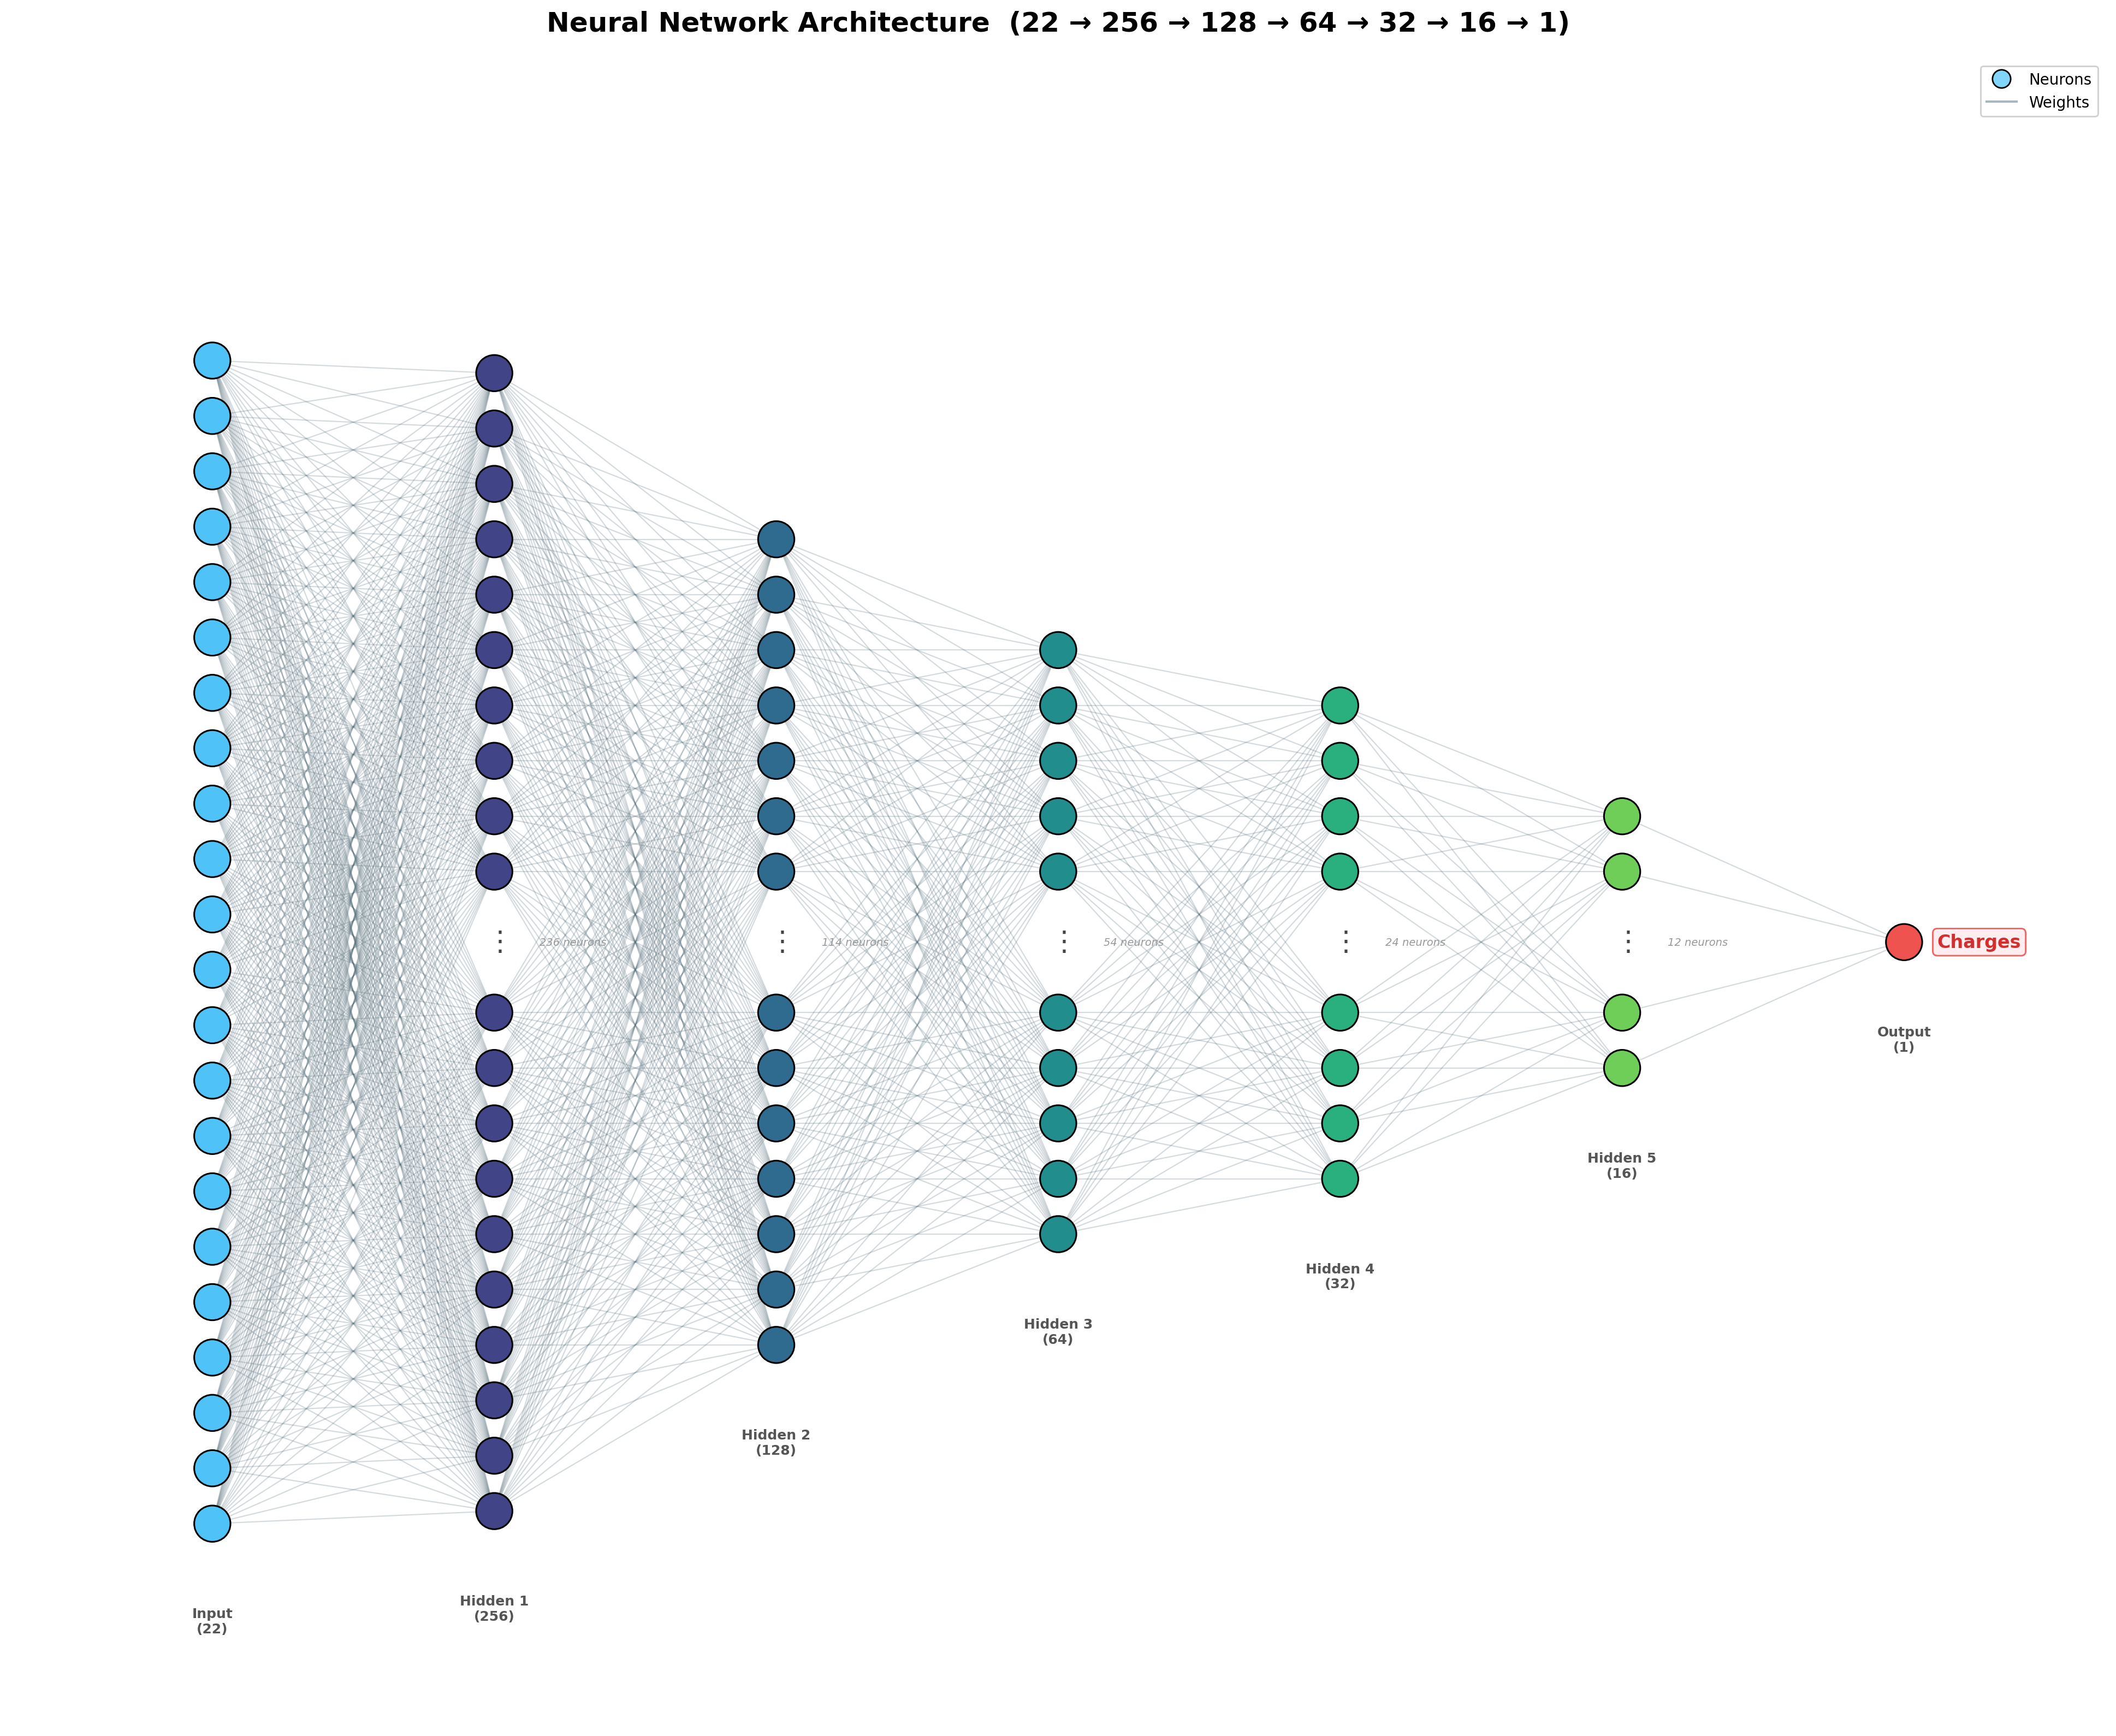
\includegraphics[width=0.85\textwidth]{Thesis/Chapter 2/Figures/nn_architecture (1).png}
    \caption{Candidate DNN architecture.}
    \label{fig:dnn_architecture}
\end{figure}

\noindent
The final output neuron represents the predicted health insurance charge or
premium. This architecture starts with a wide hidden layer and progressively
compresses the representation through successive layers, allowing the network to
learn nonlinear representations before reducing them to a scalar prediction.

\noindent
The architecture used in the empirical chapter may be implemented without
explicit bias vectors, depending on the final modelling choice confirmed for the
study. In that case, the layer recursion in
equations~\eqref{eq:pre_activation}-\eqref{eq:activation} simplifies to
\begin{equation}
\label{eq:bias_free_recursion}
    \mathbf{z}^{(l)}_i
    =
    \left(W^{(l)}\right)^{\top}
    \mathbf{a}^{(l-1)}_i,
    \qquad
    \mathbf{a}^{(l)}_i
    =
    \sigma_l
    \!\left(
        \mathbf{z}^{(l)}_i
    \right),
    \qquad
    l=1,\ldots,L,
\end{equation}
\equationlistentry{Layer recursion without bias}
with \(\mathbf{a}^{(0)}_i = \mathbf{x}_i\) as in
equation~\eqref{eq:input_layer}. The output prediction is then
\[
    f_{\theta}(\mathbf{x}_i)
    =
    a^{(L)}_{i1}.
\]
This bias-free specification removes additive layer-bias parameters from the
network architecture; the distinction between architectural, statistical and
data-related meanings of bias is noted above. Its adequacy is assessed empirically
through training, validation and test performance, and where appropriate through
comparison with a bias-inclusive network. One theoretical qualification should
be recorded. The approximation theorems reviewed in
Section~\ref{sec:dnn_regression} assume affine layer maps comprising both
weights and biases; a bias-free network whose activation satisfies
\(\sigma(0)=0\) is positively homogeneous and constrained to pass through the
origin of the standardised input space, so the universal approximation
guarantee does not directly apply to the implemented architecture.

\noindent
The final architecture should not be selected purely by intuition; it should be
determined using validation performance and evaluated on a held-out test set.
This is necessary because neural networks can be highly flexible. A network that
is too small may underfit, while a network that is too large may fit the
training data closely without generalising to unseen observations. The
DNN is therefore treated as a statistical learning model whose usefulness
is judged by out-of-sample prediction performance and by the quality of the
subsequent simulation and interpretability analysis
\citep{james2021introduction,hastie2009elements}.

\noindent
The dataset is partitioned as
\begin{equation}
\label{eq:data_partition}
    \mathcal{D}
    =
    \mathcal{D}_{\mathrm{train}}
    \cup
    \mathcal{D}_{\mathrm{val}}
    \cup
    \mathcal{D}_{\mathrm{test}},
\end{equation}
\equationlistentry{Training, validation and test partition}
where the three components are disjoint and exhaust \(\mathcal{D}\).  The
proportions allocated to each component are a design choice rather than a
fixed convention; the split used in this dissertation is stated in
Section~\ref{sec:feature_encoding_input_standardisation}. An epoch is one
complete pass through the training data. For a fitted parameter vector
\(\widehat{\theta}^{(e)}\) after epoch \(e\), the training and validation losses
are
\begin{equation}
\label{eq:training_loss_epoch}
    \mathcal{L}_{\mathrm{train}}^{(e)}
    =
    \frac{1}{n_{\mathrm{train}}}
    \sum_{i\in\mathcal{I}_{\mathrm{train}}}
    \left(
        y_i
        -
        f_{\widehat{\theta}^{(e)}}(\mathbf{x}_i)
    \right)^2
\end{equation}
\equationlistentry{Training loss at epoch $e$}
and
\begin{equation}
\label{eq:validation_loss_epoch}
    \mathcal{L}_{\mathrm{val}}^{(e)}
    =
    \frac{1}{n_{\mathrm{val}}}
    \sum_{i\in\mathcal{I}_{\mathrm{val}}}
    \left(
        y_i
        -
        f_{\widehat{\theta}^{(e)}}(\mathbf{x}_i)
    \right)^2.
\end{equation}
\equationlistentry{Validation loss at epoch $e$}
The candidate number of epochs is selected by comparing validation loss over the
epoch grid. If \(\mathcal{E}\) denotes the set of candidate epoch values, the
selected training duration is
\begin{equation}
\label{eq:epoch_selection}
    e^{\ast}
    =
    \arg\min_{e\in\mathcal{E}}
    \mathcal{L}_{\mathrm{val}}^{(e)}.
\end{equation}
\equationlistentry{Optimal epoch selection}
This validation step is necessary because training loss typically decreases as
the optimiser continues updating the model, but validation loss may eventually
increase if the network begins to adapt too closely to the training sample. A
decreasing training loss with a rising validation loss is a common indication of
overfitting, while weak training and validation performance may indicate
underfitting or unsuitable training settings.

\noindent
LOOCV is not adopted as the primary validation strategy. It would require
refitting the neural network once for each observation.

\noindent
Although \(K\)-fold cross-validation is often useful when a separate validation
set is unavailable or when dependence on a single random split must be reduced,
it is not required for the main analysis because the data are already supplied
with the fixed partition in equation~\eqref{eq:data_partition}. Applying
\(K\)-fold cross-validation to the full dataset would mix observations assigned
to validation and test components into the training process, weakening the
interpretation of the final test performance. Applying \(K\)-fold
cross-validation only to the training set would avoid this leakage, but would
require repeated DNN training across folds and candidate epoch values,
while the supplied validation set already provides the intended mechanism for
selecting the training duration. The validation analysis therefore uses the
pre-specified validation set to select \(e^{\ast}\), and the test set is used
only once for final model assessment.

% --------------------------------------------------------
% 2.4.3 Generalisation, Validation Analysis and
%       Bias-Variance Trade-off
% --------------------------------------------------------
\subsubsection{Generalisation, validation analysis and bias-variance trade-off}
\label{sec:generalisation_validation_bias_variance}

\noindent
The tension between overfitting and underfitting is particularly acute for
flexible models such as DNNs, which may contain many trainable
parameters and can represent complex nonlinear relationships. The formal
bias-variance decomposition below makes this trade-off precise.

\noindent
Expressing the regression formulation in equation~\eqref{eq:regression} in
population-level notation,
\begin{equation}
\label{eq:general_regression}
    Y
    =
    f(\mathbf{X})
    +
    \varepsilon,
\end{equation}
\equationlistentry{Population regression formulation}
where \(f(\mathbf{X})\) denotes the true regression function
\(m(\cdot)\) from equation~\eqref{eq:regression} and \(\varepsilon\) represents
irreducible noise with \(\mathbb{E}(\varepsilon\mid\mathbf{X})=0\). In the
homoscedastic case, the irreducible variation is denoted
\(\sigma_{\varepsilon}^{2}\).

\noindent
If \(\widehat{f}_{\mathcal{D}}\) is a model trained on a dataset
\(\mathcal{D}\), then prediction error on a new observation depends not only on
how well the model fits the observed data, but also on how stable the fitted
function is across different possible training samples. This motivates the
bias-variance trade-off in statistical learning
\citep{hastie2009elements,james2021introduction,bishop2006pattern}.

\noindent
For squared-error loss, the expected prediction error at a point
\(\mathbf{x}\) can be decomposed into three components:
\begin{equation}
\label{eq:bias_variance_pointwise}
\mathbb{E}_{\mathcal{D},Y}
\!\left[
\left(
Y - \widehat{f}_{\mathcal{D}}(\mathbf{x})
\right)^2
\right]
=
\underbrace{\left(
f(\mathbf{x})
-
\mathbb{E}_{\mathcal{D}}
\!\left[
\widehat{f}_{\mathcal{D}}(\mathbf{x})
\right]
\right)^2}_{\mathrm{Bias}^{2}}
+
\underbrace{
\mathbb{E}_{\mathcal{D}}
\!\left[
\left(
\widehat{f}_{\mathcal{D}}(\mathbf{x})
-
\mathbb{E}_{\mathcal{D}}
\!\left[
\widehat{f}_{\mathcal{D}}(\mathbf{x})
\right]
\right)^2
\right]
}_{\mathrm{Variance}}
+
\underbrace{\sigma_{\varepsilon}^{2}}_{\mathrm{Noise}}.
\end{equation}
\equationlistentry{Pointwise bias-variance decomposition}
The bias term measures the systematic error introduced by the choice of model
class, while the variance term measures the instability of the fitted model
across different training samples. The noise term
\(\sigma_{\varepsilon}^{2}\) represents irreducible variation in the response
that cannot be removed by any model based on the available predictors.

\noindent
The bias-variance trade-off can therefore be summarised as
\[
    \mathrm{Expected\ test\ error}
    =
    \mathrm{Variance}
    +
    \mathrm{Bias}^{2}
    +
    \mathrm{Irreducible\ noise}.
\]
Equivalently, in terms of model complexity,
\[
    \mathrm{Model\ complexity}\uparrow
    \quad
    \Longrightarrow
    \quad
    \mathrm{Bias}^{2}\downarrow,
    \qquad
    \mathrm{Variance}\uparrow,
\]
whereas
\[
    \mathrm{Model\ complexity}\downarrow
    \quad
    \Longrightarrow
    \quad
    \mathrm{Bias}^{2}\uparrow,
    \qquad
    \mathrm{Variance}\downarrow.
\]
This relationship explains why a highly flexible model may fit the training data
closely but perform poorly on unseen observations, while an overly simple model
may fail to capture the underlying pattern in both training and unseen data. The
aim is not to minimise training error alone, but to find a level of model
complexity that gives a favourable balance between bias and variance.

\begin{figure}[H]
    \centering
    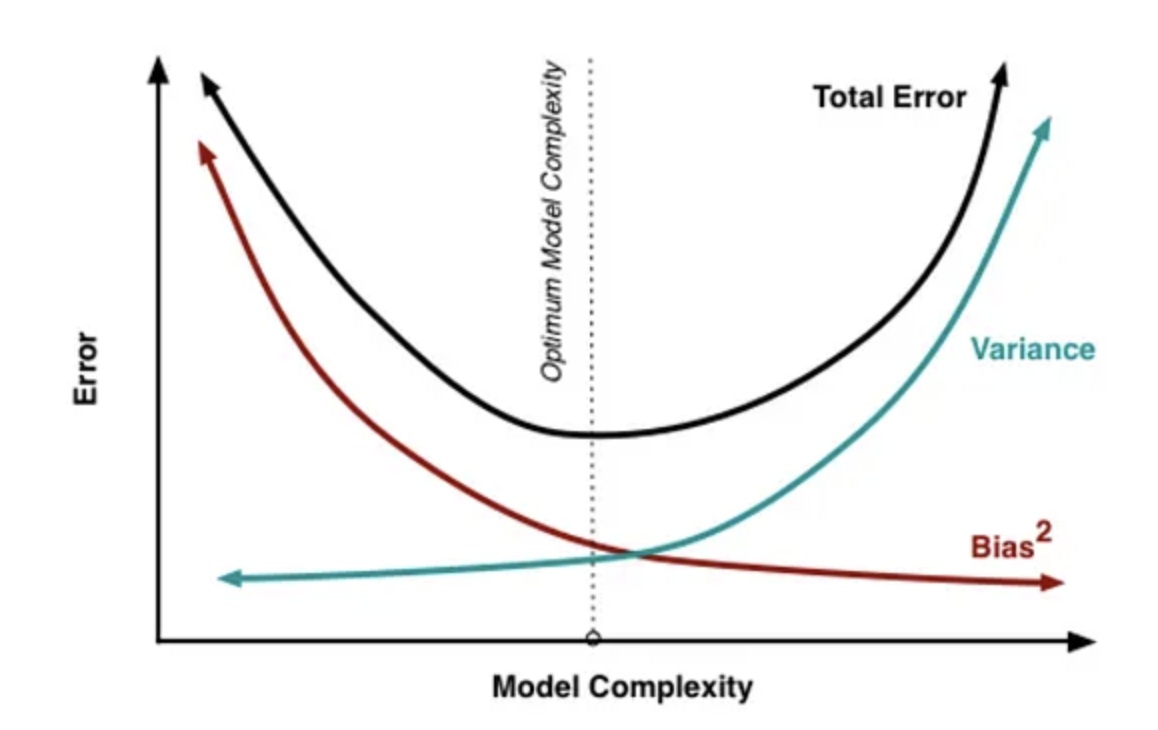
\includegraphics[width=0.72\textwidth]{Thesis/Chapter 2/Figures/bias_variance_tradeoff.png}
    \caption{Bias-variance trade-off illustration \citep{james2021introduction}.}
    \label{fig:bias_variance_tradeoff}
\end{figure}

\noindent
Figure~\ref{fig:bias_variance_tradeoff} provides a schematic illustration of
this relationship. The diagram emphasises that neither a very simple model nor
an excessively flexible model is generally desirable for prediction. Instead,
the preferred model complexity is the one that achieves the best out-of-sample
performance by balancing bias and variance. This principle motivates the
epoch-selection criterion defined in equation~\eqref{eq:epoch_selection}.

\noindent
The pointwise squared-error decomposition in
equation~\eqref{eq:bias_variance_pointwise} separates the expected prediction
error at a fixed input value \(\mathbf{x}\) into bias, variance and irreducible
noise. The same principle can also be expressed at the population level by
considering expected out-of-sample error. Let \(g^{(\mathcal{D})}\) denote a
fitted model obtained from a training sample \(\mathcal{D}\), and define the
average fitted model by
\[
    \bar{g}(\mathbf{x})
    =
    \mathbb{E}_{\mathcal{D}}
    \!\left[
        g^{(\mathcal{D})}(\mathbf{x})
    \right].
\]
Also let
\[
    m(\mathbf{X})
    =
    f(\mathbf{X})
    =
    \mathbb{E}(Y\mid \mathbf{X})
\]
denote the systematic component of the response, written with the
regression-function symbol \(m(\cdot)\) of equation~\eqref{eq:regression}
to avoid confusion with the bar notation used elsewhere for sample means. The expected out-of-sample
error under squared loss can then be written as
\begin{equation}
\label{eq:bias_variance_population}
\begin{aligned}
    \mathbb{E}_{\mathcal{D}}
    \!\left[
        E_{\mathrm{out}}
        \!\left(
            g^{(\mathcal{D})}
        \right)
    \right]
    &=
    \mathbb{E}_{\mathcal{D}}
    \!\left[
        \mathbb{E}_{\mathbf{X},Y}
        \!\left[
            \left(
                g^{(\mathcal{D})}(\mathbf{X}) - Y
            \right)^2
        \right]
    \right]
    \\[4pt]
    &=
    \underbrace{
    \mathbb{E}_{\mathbf{X}}
    \!\left[
        \mathbb{E}_{\mathcal{D}}
        \!\left[
            \left(
                g^{(\mathcal{D})}(\mathbf{X})
                -
                \bar{g}(\mathbf{X})
            \right)^2
        \right]
    \right]
    }_{\mathrm{Model\ variance}}
    \\[4pt]
    &\quad+
    \underbrace{
    \mathbb{E}_{\mathbf{X}}
    \!\left[
        \left(
            \bar{g}(\mathbf{X})
            -
            f(\mathbf{X})
        \right)^2
    \right]
    }_{\mathrm{Model\ bias}}
    +
    \underbrace{
    \mathbb{E}_{\mathbf{X}}
    \!\left[
        \mathbb{E}_{Y\mid\mathbf{X}}
        \!\left[
            \left(
                m(\mathbf{X})
                -
                Y
            \right)^2
        \right]
    \right]
    }_{\mathrm{Noise}}.
\end{aligned}
\end{equation}
\equationlistentry{Population expected prediction error}
This form is useful because it links model complexity directly to expected
out-of-sample performance, which is the quantity approximated by the validation
and test-set analysis. Complex models may reduce model bias by representing
richer patterns, but they may also increase model variance by becoming sensitive
to the particular training sample. Simpler models may have lower variance, but
they may miss important nonlinear structure. The practical aim is therefore to
choose a model that captures stable structure without merely recalling noise in
the training data.

\noindent
The training partition \(\mathcal{D}_{\mathrm{train}}\)
(equation~\eqref{eq:data_partition}) is used to estimate model parameters through
gradient-based optimisation. The validation partition
\(\mathcal{D}_{\mathrm{val}}\) guides the choice of training duration via
the epoch-selection criterion in equation~\eqref{eq:epoch_selection}. The test partition
\(\mathcal{D}_{\mathrm{test}}\) is reserved for final out-of-sample evaluation
after the model has been selected and its architecture fixed. Using the test set
for any model-selection decision invalidates its role as an honest estimate of
generalisation performance
\citep{hastie2009elements,abu2012learning}.

\noindent
Generalisation is assessed by comparing training, validation and test
performance using RMSE, MAE and \ensuremath{R^2}. If
training performance is substantially better than validation or test
performance, this may indicate overfitting. If all three are weak, this may
indicate underfitting. If training, validation and test results are similar and
sufficiently strong, this supports the conclusion that the fitted model
generalises reasonably well within the available dataset.

\noindent
The use of a benchmark health insurance dataset introduces an additional
qualification: internal predictive validity within the dataset's
distributional domain must be distinguished from external validity for
real insurance populations with different risk profiles, benefit
structures or demographics.  The scope delimitations of
Section~\ref{sec:scope_delimitations} formalise this boundary.

\newpage
% =============================================================
% 2.5  Health Insurance Pricing and Cost Prediction
% =============================================================

\subsection{Health Insurance Pricing and Cost Prediction}
\label{sec:health_insurance_pricing_cost_prediction}

\noindent
The supervised-regression formulation gives the
statistical form of the empirical problem: the observed response \(y_i\) is a
continuous monetary outcome, and the fitted function
\(\widehat{m}(\mathbf{x})\) maps policyholder attributes to a predicted cost.
The health insurance setting gives this regression problem its actuarial
meaning. A predicted monetary outcome is not merely an abstract response
variable; it is connected to premium rating, claim-cost estimation and risk
segmentation. Classical actuarial pricing often relies on transparent
regression-based models, especially GLMs, while the
DNN considered here plays the related role of a flexible nonlinear
estimator of the cost surface rather than a replacement for actuarial reasoning.

\noindent
The broader actuarial machine-learning literature provides extensive evidence
that neural networks and related models can be embedded within traditional
insurance frameworks.  \citet{wuthrich2023statistical} provide a comprehensive
treatment of statistical foundations for actuarial learning,
\citet{noll2020case} demonstrate neural-network pricing on French motor
third-party liability data, and \citet{schelldorfer2019nesting} show how
classical actuarial models can be nested within neural-network architectures.
\citet{blierwong2021machine} survey machine-learning applications across
property and casualty insurance pricing and reserving.  In the life insurance
domain, \citet{blomerus2025longterm} demonstrates the viability of deep
learning for long-term life insurance valuations using commercial European
portfolio data, achieving valuations sufficiently accurate to support
capital calculations under Solvency~II; the 99.5\% figure in that
framework is the confidence level of the one-year Value-at-Risk defining
the Solvency Capital Requirement, rather than a prescribed valuation
accuracy standard.

\noindent
Within health insurance specifically, recent work has demonstrated that neural
networks can be incorporated into actuarial pricing structures without
abandoning the underlying frequency-severity logic.
\citet{laporta2025neural} propose neural-network models for pricing correlated
health risks by embedding negative multinomial
neural networks for claim frequency and gamma neural networks for claim
severity within a classical frequency-severity structure. Their empirical
results on real-world health insurance data show that neural-network models
achieve lower out-of-sample deviance and better risk diversification than
established regression methods such as GLMs, as measured
by the ABC lift metric. The relevance of this work is that neural networks need
not be treated as generic black-box alternatives; they can be incorporated
within actuarial pricing logic to improve both accuracy and risk segmentation.

\noindent
A complementary approach to neural-network pricing is to impose explicit shape
constraints during training.  \citet{richman2024icenet} develop the ICEnet,
which adds smoothness and monotonicity penalty terms to the loss function so
that the network's ICE outputs vary in a manner
consistent with actuarial domain knowledge.  Applied to claims frequency
prediction on the French motor third-party liability dataset, the ICEnet
achieves a test-set Poisson deviance within $0.0001$ of the unconstrained
network, demonstrating that actuarial reasonableness can be enforced with
negligible accuracy cost.  Because the ICEnet targets count data under a
Poisson deviance criterion, its results are not directly comparable with the
continuous monetary cost predictions in the present dissertation; a
methodological comparison is presented in
Section~\ref{sec:comparison_constrained_nn}.

\noindent
Alongside neural-network approaches, tree-based ensemble methods have become
widely used for insurance cost prediction on structured tabular data.
\citet{orji2024explainable} apply RFs and gradient-boosted trees to
health insurance cost data and report predictive performance comparable to, and
in some configurations exceeding, that of neural networks.  More broadly,
\citet{grinsztajn2022why} provide systematic evidence that tree-based models,
particularly gradient-boosted implementations such as XGBoost
\citep{chen2016xgboost}, building on the gradient boosting framework of
\citet{friedman2001greedy}, frequently match or outperform DNNs
on
medium-sized tabular datasets of the kind encountered in actuarial practice.
Because insurance cost prediction is fundamentally an actuarial problem defined
on structured policyholder attributes rather than on unstructured data such as
images or text, tree-based methods represent a credible alternative to the
DNN and may in some settings be the preferred model class.  The present
dissertation nonetheless selects the DNN as the primary model for the
MC and Shapley workflow because it provides a differentiable
prediction surface compatible with gradient-based SHAP explainers and
with continuous forward-pass evaluation over large simulated input samples;
the specific gradient-based explainer employed is described in
Chapter~\ref{chap:methods_and_data}.  An RF
and an XGBoost regressor are fitted as benchmarks to contextualise the
DNN's predictive performance within this spectrum of model classes.

\noindent
Earlier work on algorithmic health cost prediction by
\citet{bertsimas2008algorithmic} demonstrated the potential of machine-learning
methods to outperform traditional actuarial approaches, while
\citet{duncan2016testing} tested alternative regression frameworks for
predictive modelling of healthcare costs in the North American context.
These studies confirm that health insurance cost prediction is a well-studied
regression problem where model flexibility can yield meaningful improvements
over simpler specifications.

\noindent
The available Kaggle insurance data \citep{kaggleInsuranceDataML} do not provide separate claim-frequency and
claim-severity processes. A separate actuarial claims model is therefore not
fitted. Instead, the observed monetary response is treated as an aggregate
health insurance charge or premium proxy, and cost prediction is formulated as a
supervised regression problem. This gives a narrower empirical objective: to
study how a fitted nonlinear prediction surface behaves on a benchmark
health insurance dataset, without claiming to reproduce the complete pricing
tariff or underwriting rules of a specific insurer.

\noindent
The objective is not merely to obtain a point estimate of cost for each
policyholder, but to understand the distribution and drivers of predicted costs
under varying input profiles. This is important because actuarial modelling is
concerned not only with average prediction, but also with uncertainty,
high-cost scenarios and the interpretation of risk drivers
\citep{denuit2007actuarial}. In this sense, the fitted regression function
\(\widehat{m}\) is the starting point for a broader analysis of predicted-cost
behaviour rather than the end of the modelling exercise.

\noindent
Health expense projection literature provides a further actuarial motivation for studying predicted costs distributionally. \citet{christiansen2018projection}
develop practical models for projecting health insurance expenditures over
short time horizons, which supports the view that health cost analysis should
consider the behaviour of cost outcomes beyond isolated point estimates. The
present dissertation differs from traditional health expense projection because
it does not construct a demographic, utilisation or claims-process model.
Instead, it trains a DNN on policyholder-level attributes and uses Monte
Carlo input simulation to examine the distribution of costs implied by the
fitted prediction function. This distinction keeps the empirical claim modest:
the analysis concerns model-implied predicted costs under the selected
benchmark-data and simulation design, rather than realised expenditure
dynamics in an insurer's full portfolio.

\noindent
Ordinary cost prediction is therefore extended in two ways. First, after fitting
the DNN, MC input simulation is used to generate many
possible policyholder profiles and examine the distribution of model-implied
predicted costs. Second, Shapley-value interpretation is used to identify the
variables that drive individual predictions and high-cost simulated profiles.
This connects health insurance cost prediction with simulation-based risk
analysis and explainable machine learning. The resulting analysis asks not only
how accurately the fitted model predicts costs, but also how predicted costs
vary across simulated profiles and which variables the model attributes to the
upper tail of the predicted-cost distribution.

\noindent
The interpretation remains model-based: the MC distribution describes
variation in fitted predictions under the selected input distribution, and
Shapley values explain the fitted DNN's predictions relative to the
chosen background distribution.  The causal and scope delimitations stated in
Section~\ref{sec:scope_delimitations} apply throughout.  The health insurance
application is therefore used as an actuarially motivated setting in which
prediction, simulation and explanation can be combined while keeping the
empirical claims within the limits of the data.


\newpage

% =============================================================
% 2.6  Input Distribution Diagnostics for Simulation
% =============================================================

\subsection{Input Distribution Diagnostics for Simulation}
\label{sec:input_distribution_diagnostics}

\noindent
The validation analysis of
Section~\ref{sec:generalisation_validation_bias_variance} addresses whether
the fitted DNN generalises within the supplied
training, validation and test structure, but MC input simulation requires an
additional diagnostic step. Even when a fitted prediction function
\(f_{\widehat{\theta}}\) has acceptable validation and test performance, the
simulation results may be misleading if the input profiles are generated from an
unrealistic or poorly specified input distribution. The diagnostic concern
therefore shifts from the fitted model itself to the probability law used to
generate simulated policyholder profiles.

\noindent
A trained model \(f_{\widehat{\theta}}\) can be evaluated at any admissible
input vector, but simulation-based analysis requires a probability law for the
random input vector \(\mathbf{X}\). The distribution of simulated predictions
depends not only on the fitted DNN, but also on the assumed or estimated
distribution of policyholder attributes. Input distribution diagnostics therefore
provide the empirical basis for specifying the input distribution
\(\widehat{F}_{X}\) used later in the MC component of the framework.

\noindent
Let
\[
    \mathbf{X}
    =
    (X_1,\ldots,X_p)^{\top}
\]
denote the vector of input variables before final model encoding, and let
\(\widetilde{\mathbf{X}}\) denote the corresponding model-ready vector after
encoding and standardisation. Where no ambiguity arises, \(\mathbf{X}\) is used
as the generic random input vector. Before specifying an input distribution for
\(\mathbf{X}\), the empirical distribution of each variable must be examined.
For numerical variables, this includes measures of location, scale, skewness,
tail behaviour and possible outliers. For categorical variables, this includes
category frequencies, rare levels and possible class imbalance.

\noindent
For a numerical variable \(X_j\), the sample mean and variance are
\[
    \bar{x}_j
    =
    \frac{1}{n}
    \sum_{i=1}^{n}
    x_{ij},
    \qquad
    s_j^2
    =
    \frac{1}{n-1}
    \sum_{i=1}^{n}
    \left(
        x_{ij} - \bar{x}_j
    \right)^2.
\]
Skewness can be estimated by
\[
    \widehat{\gamma}_{1j}
    =
    \frac{
    \frac{1}{n}\sum_{i=1}^{n}
    \left(
        x_{ij}-\bar{x}_j
    \right)^3
    }{
    \left[
    \frac{1}{n}\sum_{i=1}^{n}
    \left(
        x_{ij}-\bar{x}_j
    \right)^2
    \right]^{3/2}
    },
\]
and kurtosis by
\[
    \widehat{\gamma}_{2j}
    =
    \frac{
    \frac{1}{n}\sum_{i=1}^{n}
    \left(
        x_{ij}-\bar{x}_j
    \right)^4
    }{
    \left[
    \frac{1}{n}\sum_{i=1}^{n}
    \left(
        x_{ij}-\bar{x}_j
    \right)^2
    \right]^2
    }.
\]
Following common convention, the sample variance \(s_j^2\) uses the
unbiased divisor \(n-1\), whereas the skewness and kurtosis estimators are
ratios of divisor-\(n\) central moments; this mixed convention is adopted
throughout. Values of \(\widehat{\gamma}_{1j}>0\) indicate right-skewness, while values of
\(\widehat{\gamma}_{2j}\) substantially above \(3\) indicate heavier-than-normal
tails. These quantities help identify variables that are asymmetric,
heavy-tailed or potentially unsuitable for simple symmetric distributional
assumptions.

\noindent
The response variable \texttt{charges} is also subject to diagnostic analysis,
even though MC input simulation focuses primarily on the predictors.
Insurance cost variables often display right-skewness, heterogeneity and
upper-tail behaviour \citep{denuit2007actuarial}. If the response is strongly
skewed, a log transformation of the form
\[
    Y_i^{*}
    =
    \log(1+Y_i)
\]
may be considered during model training. If such a transformation is used, final
predictions and performance metrics must be back-transformed and reported on the
original monetary scale.

\noindent
For categorical variables, the relevant diagnostic is the empirical frequency
distribution. If \(X_j\) takes values in the finite set
\(\{c_1,\ldots,c_{K_j}\}\), the empirical proportion of category \(c_k\) is
\[
    \widehat{p}_{jk}
    =
    \frac{1}{n}
    \sum_{i=1}^{n}
    \mathbb{I}\{X_{ij}=c_k\}.
\]
Rare categories may be poorly represented in the training set and may lead to
unstable predictions or unreliable Shapley summaries. In the health insurance
setting, categorical variables such as region, smoking status, medical history,
exercise frequency, occupation and coverage level may all influence the
structure learned by the fitted model.

\noindent
Input diagnostics also inform preprocessing. Numerical variables are
standardised before training a DNN to support numerical stability in
gradient-based optimisation. The standardisation parameters must be computed from
the training set only and then applied to the validation and test sets using
those same training-set values, so that information from held-out observations
does not leak into the training procedure. The specific standardisation formula
and its implementation are detailed in Chapter~\ref{chap:methods_and_data}.

\noindent
Validation analysis assesses whether
\(f_{\widehat{\theta}}\) performs adequately on held-out observations from the
available data distribution. Input distribution diagnostics assess whether the
profiles generated for MC simulation remain compatible with that same
empirical domain. Without both checks, the subsequent predicted-cost
distribution and high-cost Shapley summaries could reflect unrealistic simulated
profiles rather than meaningful behaviour of the fitted model.

% =============================================================
% 2.7  Specification of the Input Distribution
% =============================================================

\subsection{Specification of the Input Distribution}
\label{sec:input_simulation_uncertainty_dependence}

\noindent
The input distribution
\(\widehat{F}_{X}\) was defined as a product of independent fitted marginals
(equation~\eqref{eq:input_law}), with the sampling and propagation
procedure given by equations~\eqref{eq:mc_sample_framework}
and~\eqref{eq:mc_predictions_framework}. Three main
approaches are available for constructing \(\widehat{F}_{X}\).

\noindent
The simplest approach is empirical row resampling, in which complete observed
covariate vectors are sampled from the dataset with replacement
\citep{efron1993bootstrap}:
\begin{equation}
\label{eq:row_resampling}
    \mathbf{X}^{(\ell)}
    \in
    \{\mathbf{x}_1,\ldots,\mathbf{x}_n\},
    \qquad
    \ell=1,\ldots,M.
\end{equation}
\equationlistentry{Empirical row resampling}
Because the full covariate vector is sampled as a unit, empirical row resampling
retains whatever joint structure is present in the observed data. Its limitation
is that it cannot generate policyholder profiles outside the observed data
range.

\noindent
A second approach is marginal parametric simulation, in which each input
variable is assigned a fitted marginal distribution
\citep{rubinstein2016simulation,glasserman2004monte}. For a numerical variable
\(X_j\), a parametric family \(F_j(\,\cdot\,;\psi_j)\) may be fitted by maximum
likelihood:
\begin{equation}
\label{eq:mle_marginal}
    \widehat{\psi}_j
    =
    \arg\max_{\psi_j}
    \sum_{i=1}^{n}
    \log f_j(x_{ij};\psi_j),
\end{equation}
\equationlistentry{Maximum likelihood for marginal parameters}
where \(f_j(\cdot;\psi_j)\) is the corresponding density or probability mass
function. Simulated values are then drawn as
\begin{equation}
\label{eq:marginal_draw}
    X_j^{(\ell)}
    \sim
    F_j(\,\cdot\,;\widehat{\psi}_j),
    \qquad
    \ell=1,\ldots,M.
\end{equation}
\equationlistentry{Draw from fitted marginal distribution}
This approach is convenient and can generate values beyond the observed sample.
It is the approach adopted in this dissertation, where independent fitted
marginals are combined as specified in equation~\eqref{eq:input_law}. The
independence assumption is a deliberate modelling choice, as discussed in
connection with equation~\eqref{eq:input_law}. Two strands of literature
qualify this choice. Evaluating or explaining a fitted model at covariate
combinations that lie off the data manifold can produce extrapolation
artefacts, because the model is queried in regions where it was never
constrained by training data \citep{hooker2021unrestricted}. Relatedly, when
features are dependent, the marginal (interventional) and conditional
formulations of Shapley attribution diverge, and estimating the conditional
expectations required by the latter is non-trivial
\citep{aas2021explaining, janzing2020feature}. Under the product-marginal
design adopted here the two formulations coincide by construction, which is
precisely the condition under which the marginal SHAP estimator used
later is internally consistent. The generated profiles may nonetheless
include jointly implausible attribute combinations, so attribution results
in sparsely supported regions of the input space must be interpreted with
care.

\noindent
A third approach is nonparametric or semi-parametric simulation, using
bootstrap-type resampling or smoothed empirical distributions
\citep{efron1993bootstrap}. These methods avoid imposing a strong parametric
form on the marginal distributions, although they remain limited by the
information contained in the observed sample. Their usefulness depends on
whether the empirical data provide sufficient coverage of the regions of the
input space that are relevant for the simulation exercise.

\noindent
The choice of specification method determines the input profiles passed through
the fitted prediction function. A poorly specified input distribution may create
high-cost profiles that are artefacts of the simulation design rather than
meaningful evaluations of the fitted model.

\noindent
Figure~\ref{fig:input_law_construction} illustrates the marginal parametric
construction adopted here. Each column of \(\mathcal{X}_{\mathrm{train}}\) is
fitted independently to a parametric marginal distribution, and the product of
these marginals defines \(\widehat{F}_{X}\), from which \(M\) synthetic input
vectors are drawn to form the simulation design matrix.

\begin{figure}[H]
\centering
\begin{tikzpicture}[
    databox/.style={rectangle, draw, minimum width=2cm,
        minimum height=0.9cm, align=center, font=\small},
    prodbox/.style={rectangle, draw, rounded corners,
        minimum width=11.5cm, minimum height=1.1cm,
        align=center, font=\normalsize, fill=blue!8},
    samplebox/.style={rectangle, draw, rounded corners,
        fill=purple!5, inner sep=10pt,
        align=center, font=\small},
    arr/.style={->, thick, >=stealth}
]

\def\colA{0}
\def\colB{3}
\def\colMid{5}
\def\colC{7}
\def\colD{10}

% ROW 1 — Training attribute columns
\node[databox] (x1) at (\colA,0)
      {$\mathbf{x}_{\cdot 1}$\\{\scriptsize(age)}};
\node[databox] (x2) at (\colB,0)
      {$\mathbf{x}_{\cdot 2}$\\{\scriptsize(BMI)}};
\node[font=\large] at (\colMid,0) {$\cdots$};
\node[databox] (x3) at (\colC,0)
      {$\mathbf{x}_{\cdot(p{-}1)}$\\{\scriptsize(children)}};
\node[databox] (xp) at (\colD,0)
      {$\mathbf{x}_{\cdot p}$\\{\scriptsize(smoker)}};

\node[font=\small\bfseries] at (\colMid,1.1)
      {Training attributes $\mathcal{X}_{\mathrm{train}}$};

% ROW 2 — Fitted-marginal labels
\node[font=\small, align=center] (f1) at (\colA,-1.9)
      {$\widehat{F}_{X_1}$\\[-1pt]{\scriptsize Normal}};
\node[font=\small, align=center] (f2) at (\colB,-1.9)
      {$\widehat{F}_{X_2}$\\[-1pt]{\scriptsize Lognormal}};
\node[font=\large] at (\colMid,-1.9) {$\cdots$};
\node[font=\small, align=center] (f3) at (\colC,-1.9)
      {$\widehat{F}_{X_{p-1}}$\\[-1pt]{\scriptsize Poisson}};
\node[font=\small, align=center] (fp) at (\colD,-1.9)
      {$\widehat{F}_{X_p}$\\[-1pt]{\scriptsize Categorical}};

\draw[arr] (x1) -- node[right,font=\scriptsize]{fit} (f1);
\draw[arr] (x2) -- node[right,font=\scriptsize]{fit} (f2);
\draw[arr] (x3) -- node[right,font=\scriptsize]{fit} (f3);
\draw[arr] (xp) -- node[right,font=\scriptsize]{fit} (fp);

% ROW 3 — Mini distribution plots
\begin{scope}[shift={(\colA,-3.15)}]
    \draw[gray!50] (-1,0) -- (1,0);
    \fill[blue!12]
        plot[smooth,domain=-0.9:0.9,samples=30]
        (\x,{0.6*exp(-5*\x*\x)})
        -- (0.9,0) -- (-0.9,0) -- cycle;
    \draw[thick,blue!70]
        plot[smooth,domain=-0.9:0.9,samples=30]
        (\x,{0.6*exp(-5*\x*\x)});
\end{scope}

\begin{scope}[shift={(\colB,-3.15)}]
    \draw[gray!50] (-1,0) -- (1.1,0);
    \fill[red!10]
        plot[smooth,domain=-0.7:1.05,samples=30]
        (\x,{0.55*exp(-3*(\x+0.1)*(\x+0.1))
             +0.15*exp(-5*(\x-0.6)*(\x-0.6))})
        -- (1.05,0) -- (-0.7,0) -- cycle;
    \draw[thick,red!70]
        plot[smooth,domain=-0.7:1.05,samples=30]
        (\x,{0.55*exp(-3*(\x+0.1)*(\x+0.1))
             +0.15*exp(-5*(\x-0.6)*(\x-0.6))});
\end{scope}

\node[font=\large] at (\colMid,-2.95) {$\cdots$};

\begin{scope}[shift={(\colC,-3.15)}]
    \draw[gray!50] (-1,0) -- (1.15,0);
    \foreach \lx/\rx/\ht in
        {-0.7/-0.4/0.35, -0.15/0.15/0.55,
         0.4/0.7/0.25,   0.85/1.05/0.08}{
        \fill[green!40] (\lx,0) rectangle (\rx,\ht);
        \draw[green!60!black] (\lx,0) rectangle (\rx,\ht);
    }
    \foreach \xv/\lab in {-0.55/0, 0/1, 0.55/2, 0.95/3}
        \node[font=\tiny] at (\xv,-0.15) {\lab};
\end{scope}

\begin{scope}[shift={(\colD,-3.15)}]
    \draw[gray!50] (-0.85,0) -- (0.85,0);
    \fill[yellow!50]   (-0.65,0) rectangle (-0.1,0.55);
    \draw[yellow!60!black] (-0.65,0) rectangle (-0.1,0.55);
    \fill[yellow!50]   (0.1,0) rectangle (0.65,0.2);
    \draw[yellow!60!black] (0.1,0) rectangle (0.65,0.2);
    \node[font=\tiny] at (-0.375,-0.15) {No};
    \node[font=\tiny] at ( 0.375,-0.15) {Yes};
\end{scope}

% ROW 4 — Product of independent marginals
\node[prodbox] (FX) at (\colMid,-4.85)
      {$\displaystyle\widehat{F}_{X}
        \;=\;\prod_{j=1}^{p}\widehat{F}_{X_j}$};

\draw[arr] (\colA,-3.55) -- (FX.north -| \colA,0);
\draw[arr] (\colB,-3.55) -- (FX.north -| \colB,0);
\draw[arr] (\colC,-3.55) -- (FX.north -| \colC,0);
\draw[arr] (\colD,-3.55) -- (FX.north -| \colD,0);

\node[below=0.2cm of FX, font=\scriptsize\itshape] (indep)
      {(independent marginals; no copula structure)};

% ROW 5 — Sampled design matrix
\draw[arr] (indep.south) ++(0,-0.15) -- ++(0,-0.8)
      node[midway,right,font=\scriptsize]{sample $M$ vectors};

\node[samplebox] at (\colMid,-8.6)
      {$\underbrace{%
       \begin{pmatrix}
       x_1^{(1)} & x_2^{(1)} & \cdots & x_p^{(1)}\\[3pt]
       x_1^{(2)} & x_2^{(2)} & \cdots & x_p^{(2)}\\[1pt]
       \vdots    & \vdots    & \ddots & \vdots   \\[1pt]
       x_1^{(M)} & x_2^{(M)} & \cdots & x_p^{(M)}
       \end{pmatrix}
       }_{\displaystyle
         \mathcal{X}_{\mathrm{sim}}\;\in\;\mathbb{R}^{M\times p}}$};

\end{tikzpicture}
\caption{Construction of the input distribution $\widehat{F}_{X}$.}
\label{fig:input_law_construction}
\end{figure}

% =============================================================
% 2.8  Foundations of MC
% =============================================================

\subsection{Foundations of MC}
\label{sec:monte_carlo_foundations}

\noindent
MC simulation rests on a small number of foundational results
concerning the crude MC estimator, its convergence
properties and the precision measures that underpin the analysis
\citep{glasserman2004monte, rubinstein2016simulation, robert2004monte,
kroese2011handbook}.

\noindent
Let \(X\) be a random variable with distribution \(F\), and suppose that the
quantity of interest is
\begin{equation}
\label{eq:mc_target}
    \theta
    =
    \mathbb{E}[g(X)].
\end{equation}
\equationlistentry{Target quantity as expectation}
If
\begin{equation}
\label{eq:mc_iid_sample}
    X^{(1)},\ldots,X^{(M)}
    \stackrel{\mathrm{iid}}{\sim}
    F,
\end{equation}
\equationlistentry{IID sample from distribution $F$}
then the crude MC estimator of \(\theta\) is
\begin{equation}
\label{eq:mc_estimator}
    \widehat{\theta}_{M}
    =
    \frac{1}{M}
    \sum_{\ell=1}^{M}
    g
    \!\left(
        X^{(\ell)}
    \right).
\end{equation}
\equationlistentry{Crude MC estimator}
Under standard regularity conditions, the law of large numbers implies
\begin{equation}
\label{eq:mc_lln}
    \widehat{\theta}_{M}
    \longrightarrow
    \theta
    \qquad
    \text{as}
    \qquad
    M\longrightarrow\infty.
\end{equation}
\equationlistentry{Law of large numbers for MC}
If
\begin{equation}
\label{eq:mc_variance_condition}
    \sigma_g^2
    =
    \mathrm{Var}\{g(X)\}
    <
    \infty,
\end{equation}
\equationlistentry{Variance condition for $g(X)$}
then
\begin{equation}
\label{eq:mc_estimator_variance}
    \mathrm{Var}
    \!\left(
        \widehat{\theta}_{M}
    \right)
    =
    \frac{\sigma_g^2}{M},
\end{equation}
\equationlistentry{Variance of MC estimator}
which yields the familiar \(M^{-1/2}\) convergence rate of ordinary MC
simulation \citep{caflisch1998monte,glasserman2004monte}.

\noindent
The MCSE quantifies the simulation error associated with
using a finite number of random draws. It is estimated by
\begin{equation}
\label{eq:mcse}
    \mathrm{MCSE}
    \!\left(
        \widehat{\theta}_{M}
    \right)
    =
    \frac{s_M}{\sqrt{M}},
\end{equation}
\equationlistentry{MCSE}
where
\begin{equation}
\label{eq:mc_sample_variance}
    s_M^2
    =
    \frac{1}{M-1}
    \sum_{\ell=1}^{M}
    \left[
        g
        \!\left(
            X^{(\ell)}
        \right)
        -
        \widehat{\theta}_{M}
    \right]^2.
\end{equation}
\equationlistentry{Sample variance for MCSE}
By the central limit theorem,
\begin{equation}
\label{eq:mc_clt}
    \frac{
        \widehat{\theta}_{M}
        -
        \theta
    }{
        s_M/\sqrt{M}
    }
    \;
    \overset{d}{\longrightarrow}
    \;
    N(0,1),
\end{equation}
\equationlistentry{Central limit theorem for MC}
giving the approximate \(100(1-\alpha)\%\) MC confidence interval
\begin{equation}
\label{eq:mc_ci}
    \widehat{\theta}_{M}
    \pm
    z_{1-\alpha/2}
    \frac{s_M}{\sqrt{M}}.
\end{equation}
\equationlistentry{MC confidence interval}
This interval describes uncertainty due to the finite number of MC
draws. It does not, by itself, represent all sources of statistical uncertainty
in the fitted DNN, the input distribution or the realised insurance cost.

\noindent
In the health insurance framework, the function \(g\) is
the fitted prediction function \(\widehat{m}\), the distribution \(F\) is the
fitted input distribution \(\widehat{F}_{X}\), and the target
\(\theta\) corresponds to summaries of the model-implied predicted-cost
distribution such as the mean, variance and upper-tail probabilities. The
convergence, variance and confidence-interval results above therefore apply
directly to those summaries.

% =============================================================
% 2.9  Variance Reduction and Tail Simulation
% =============================================================

\subsection{Variance Reduction and Tail Simulation}
\label{sec:variance_reduction_tail_simulation}

\noindent
For many quantities, ordinary MC simulation is sufficient when the
simulation budget is large and the MCSE is reported.
However, when the quantity of interest is a tail probability, a high quantile or
a rare high-cost event, crude MC can become inefficient because few
simulated draws fall in the region of interest. This issue is directly relevant
to insurance because high-cost events may be financially important even when
they are relatively rare \citep{glasserman2004monte}.  The statistical
modelling of extreme events is well developed in the quantitative risk
management literature \citep{mcneil2015quantitative, embrechts1997modelling,
coles2001introduction}, where tail behaviour is characterised through extreme
value distributions and related threshold exceedance models.

\noindent
Two clarifications situate the present tail analysis within this
literature. First, the quantity simulated here is the fitted conditional
mean \(\widehat{m}(\mathbf{X})\), so the upper tail examined is a tail of
conditional means rather than of realised costs; since
\(\mathrm{Var}\{\mathbb{E}(Y\mid\mathbf{X})\}\leq\mathrm{Var}(Y)\), this
tail is necessarily lighter than the tail of realised claim costs, and
high-cost conditioning statements therefore concern expected costs rather
than realised claim severities. Second, a fuller treatment of extremes
would adopt the peaks-over-threshold framework, in which suitably
normalised excesses over a high threshold converge to the generalised
Pareto distribution
\citep{pickands1975statistical, balkema1974residual, coles2001introduction};
fitting such threshold-exceedance models to the cost distribution is
deferred to future work.

\noindent
Let \(u\) denote a high-cost threshold, and suppose that the model-implied
exceedance probability is
\[
    p_u
    =
    \mathbb{P}
    \!\left(
        \widehat{Y}>u
    \right),
\]
where
\[
    \widehat{Y}
    =
    \widehat{m}(\mathbf{X}),
    \qquad
    \mathbf{X}
    \sim
    \widehat{F}_{X}.
\]
Given simulated predictions
\(\widehat{Y}^{(1)},\ldots,\widehat{Y}^{(M)}\), the crude MC estimator
of \(p_u\) is
\[
    \widehat{p}_u
    =
    \frac{1}{M}
    \sum_{\ell=1}^{M}
    \mathbb{I}
    \!\left\{
        \widehat{Y}^{(\ell)}>u
    \right\}.
\]
Its estimated standard error is
\[
    \widehat{\mathrm{SE}}
    \!\left(
        \widehat{p}_u
    \right)
    =
    \sqrt{
        \frac{
            \widehat{p}_u
            \left(
                1-\widehat{p}_u
            \right)
        }{
            M
        }
    }.
\]
The relative standard error is approximately
\[
    \frac{
        \widehat{\mathrm{SE}}
        \!\left(
            \widehat{p}_u
        \right)
    }{
        \widehat{p}_u
    }
    \approx
    \sqrt{
        \frac{
            1-\widehat{p}_u
        }{
            M\widehat{p}_u
        }
    }.
\]
When \(p_u\) is small, the expected number of exceedances,
\(Mp_u\), may remain small unless \(M\) is large. This explains why rare-event
estimation can be difficult under crude MC sampling.

\noindent
Importance sampling is one classical variance-reduction method. Suppose that
samples are drawn from an alternative density \(q\) rather than the original
density \(f\). For a target expectation
\[
    \theta
    =
    \int
    g(x)f(x)\,dx,
\]
the same quantity may be written as
\[
    \theta
    =
    \int
    g(x)
    \frac{f(x)}{q(x)}
    q(x)\,dx.
\]
The corresponding importance-sampling estimator is
\[
    \widehat{\theta}_{\mathrm{IS}}
    =
    \frac{1}{M}
    \sum_{\ell=1}^{M}
    g
    \!\left(
        X^{(\ell)}
    \right)
    w
    \!\left(
        X^{(\ell)}
    \right),
    \qquad
    X^{(\ell)}\sim q,
\]
where
\[
    w(x)
    =
    \frac{f(x)}{q(x)}
\]
is the likelihood ratio, also called the importance weight. For the
identity above to hold, the proposal density must satisfy \(q(x)>0\)
wherever \(g(x)f(x)\neq 0\), so that the integrand remains absolutely
continuous with respect to the proposal. A well-chosen
proposal distribution \(q\) concentrates simulation effort in the region that
contributes most to the quantity being estimated, and can substantially reduce
estimator variance \citep{glasserman2004monte,rubinstein2016simulation}. An
ill-chosen proposal, however, yields unbounded likelihood ratios and can
produce an estimator with severely inflated, or even infinite, variance, so
the proposal distribution must be selected with care.

\noindent
Stratified sampling is another variance-reduction approach. Suppose the input
space is partitioned into disjoint strata
\[
    A_1,\ldots,A_H,
\]
with
\[
    p_h
    =
    \mathbb{P}
    \!\left(
        \mathbf{X}\in A_h
    \right).
\]
If \(M_h\) samples are drawn from stratum \(h\), the stratified estimator of
\(\theta=\mathbb{E}\{g(\mathbf{X})\}\) is
\[
    \widehat{\theta}_{\mathrm{strat}}
    =
    \sum_{h=1}^{H}
    p_h
    \overline{g}_h,
\]
where \(\overline{g}_h\) is the sample mean within stratum \(h\). Its variance is
\[
    \mathrm{Var}
    \!\left(
        \widehat{\theta}_{\mathrm{strat}}
    \right)
    =
    \sum_{h=1}^{H}
    \frac{
        p_h^2\sigma_h^2
    }{
        M_h
    },
\]
where \(\sigma_h^2\) is the conditional variance of \(g(\mathbf{X})\) within
stratum \(h\). In a health insurance application, natural strata may include
smoking status, age band, BMI category, medical history group or coverage
level. Stratification is useful when these groups are expected to contribute
differently to the predicted-cost distribution \citep{rubinstein2016simulation}.

\noindent
Quasi-MC methods replace independent random points with
low-discrepancy sequences designed to cover the unit cube more evenly. If
\[
    \mathbf{u}^{(1)},\ldots,\mathbf{u}^{(M)}
    \in
    [0,1]^p
\]
are low-discrepancy points and \(T\) maps uniform vectors to input profiles, the
quasi-MC estimator is
\[
    \widehat{\theta}_{\mathrm{QMC}}
    =
    \frac{1}{M}
    \sum_{\ell=1}^{M}
    g
    \!\left(
        T
        \!\left(
            \mathbf{u}^{(\ell)}
        \right)
    \right).
\]
For integrands of bounded variation in the sense of Hardy and Krause, the
Koksma-Hlawka inequality implies that
quasi-MC methods can improve convergence relative to ordinary Monte
Carlo, with rates closer to
\[
    O
    \!\left(
        M^{-1}
        (\log M)^p
    \right)
\]
than the usual
\[
    O
    \!\left(
        M^{-1/2}
    \right)
\]
MC rate \citep{caflisch1998monte,lemieux2009monte,owen2013monte}.
At the input dimension used here, \(p=22\), the \((\log M)^{p}\) factor
renders this worst-case bound practically vacuous for feasible simulation
sizes, so any benefit of quasi-MC sampling in this setting would rest
on low effective dimension of the integrand rather than on the formal rate.

\noindent
In the present framework, variance-reduction methods are primarily relevant for
interpreting high-cost simulated profiles. The main simulation exercise may use
crude MC or empirical resampling, but the variance-reduction literature
clarifies why tail quantities require care when reporting precision. If
high-cost probabilities, upper quantiles or conditional Shapley summaries for
extreme predicted costs are estimated, the simulation size and precision of
those estimates should be reported and justified.

\noindent
A practical criterion for selecting a simulation size is a pilot-based
calculation. If \(s_0^2\) is a pilot estimate of the variance of the simulated
quantity and an absolute half-width \(\epsilon\) is desired for an approximate
confidence interval, then a rough simulation-size requirement is
\[
    M
    \;\gtrsim\;
    \left(
        \frac{
            z_{1-\alpha/2}s_0
        }{
            \epsilon
        }
    \right)^2.
\]
This expression connects the simulation budget to the desired numerical
precision of the reported MC summaries.

\noindent
Tail simulation also connects to Shapley-value
attribution. The simulated high-cost set \(\mathcal{H}_{u}\)
(equation~\eqref{eq:high_cost_set}) contains the profiles for which
feature-attribution summaries are most relevant to the upper tail of the fitted
model. Shapley values can then be used to identify which variables receive large
model-attributed contributions among simulated profiles whose fitted predictions
exceed \(u\). In this way, tail simulation provides the subset of simulated
profiles on which the high-cost interpretability analysis is based.


% =============================================================
% 2.10  Explainability, Shapley Values and Conditional Interpretation
% =============================================================

\subsection{Explainability, Shapley Values and Conditional Interpretation}
\label{sec:explainability_shapley_shap}

\noindent
DNNs are flexible nonlinear prediction models, but their flexibility often comes at the cost of interpretability. In insurance applications, this is a serious practical and regulatory concern. A model may produce accurate predictions, but insurers, regulators and policyholders may still require an explanation of why a particular profile receives a high predicted cost. This motivates the use of explainable artificial intelligence methods \citep{lundberg2017unified, molnar2022interpretable}.

\noindent
Shapley values originate in cooperative game theory and provide a principled axiomatic method for allocating a total payoff among players \citep{shapley1953value}. In machine learning, the players are the input variables and the payoff is the model prediction. The Shapley value of feature \(j\) measures the average marginal contribution of that feature across all possible subsets of features, as formalised in equation~\eqref{eq:shapley_exact}. The Shapley value is the unique solution satisfying four axioms: efficiency (contributions sum to the total prediction shift), symmetry (identically contributing features receive identical values), dummy (a feature that never changes the value receives zero), and additivity \citep{shapley1953value}.

\noindent
The SHAP framework connects Shapley values to machine learning model interpretation \citep{lundberg2017unified}. The additive decomposition in equation~\eqref{eq:shapley_decomp} provides a local explanation of an individual prediction. Within the class of additive feature attribution methods, the Shapley value is the unique attribution satisfying local accuracy (the machine-learning counterpart of the efficiency axiom above), missingness and consistency \citep[Theorem~1]{lundberg2017unified}, a result building on the uniqueness theorem of \citet{young1985monotonic}, in which a monotonicity condition takes the place of the dummy and additivity axioms of the classical characterisation. This uniqueness result is why the Shapley value constitutes the theoretical foundation for the SHAP computational framework.  \citet{covert2021explaining} provide a unifying removal-based framework that relates SHAP to other explanation methods, \citet{sundararajan2020many} examine the many distinct Shapley value formulations that arise under different baseline and feature-dependence assumptions, and \citet{lundberg2020local} extend Shapley-based explanations from local to global understanding for tree models.

\noindent
Shapley-based explanations can be interpreted locally or globally. A local explanation focuses on a single policyholder profile and explains why the model assigned a particular predicted cost. A global explanation summarises feature contributions across many observations. A common global importance measure is the mean absolute Shapley value:
\[
I_j
=
\frac{1}{n}
\sum_{i=1}^{n}
|\phi_j(\mathbf{x}_i)|.
\]
Large values of \(I_j\) indicate that feature \(j\) tends to contribute strongly to predictions across the dataset.

\noindent
In health insurance cost prediction, Shapley values can help identify whether variables such as smoking status, age, BMI, medical history, occupation, region or coverage level are driving predicted charges. The model-based interpretation caveat stated in Section~\ref{high-cost} applies equally here: Shapley contributions reflect the fitted model's attributions, not causal effects. This distinction is particularly important when working with a benchmark dataset such as the Kaggle Insurance Data for Machine Learning \citep{kaggleInsuranceDataML}, where Shapley values explain the relationships learned from the dataset's generating structure rather than from real-world pricing processes.

\noindent
The dissertation extends ordinary Shapley analysis by connecting it to
MC simulation.  Instead of computing Shapley values only on the
observed test set, attributions are also examined for simulated
policyholder profiles whose fitted predictions exceed a high-cost
threshold, using the conditional summaries \(\widehat{\Phi}_{j,u}\)
and \(\widehat{A}_{j,u}\) already formalised in
Section~\ref{high-cost}
(equations~\eqref{eq:signed_shapley_high}
and~\eqref{eq:abs_shapley_high}).  This conditional interpretation
moves beyond ordinary global feature ranking by focusing on the part of
the prediction distribution that is most relevant for insurance risk
analysis: it asks which variables contribute most strongly among
precisely those profiles that the model regards as expensive.


% =============================================================
% 2.11  Research Gap
% =============================================================

\subsection{Research Gap}
\label{sec:research_gap}

\noindent
Supervised regression provides the predictive formulation,
the DNN supplies a fitted nonlinear prediction surface, MC
simulation propagates variation in the input profiles, and Shapley values
provide feature-level attribution for fitted predictions. Each of these
components is individually well established in the statistical and
machine-learning literatures
\citep{vapnik1998statistical, friedman2001greedy, robert2004monte,
lundberg2017unified, molnar2022interpretable}.
The contribution of this dissertation is methodological: the
conditional Shapley analysis computed within Monte-Carlo-simulated
high-cost regions produces a form of threshold-conditional feature
attribution that none of these individually mature tools can deliver
in isolation.  While each component is well known, their integration
within a single, reproducible workflow provides a capability not
previously demonstrated in the health insurance cost-prediction
literature.

\noindent
MC simulation has a long history in actuarial science and quantitative
finance, where it is used primarily for loss reserving, aggregate loss
distributions, solvency capital estimation and derivative pricing
\citep{glasserman2004monte}. In these applications the simulation target is
typically a financial or insurance outcome variable, and the objective is to
estimate a distributional quantity such as a quantile or expected shortfall. The
use of MC simulation to generate a synthetic input space and propagate
it through a fitted prediction function, so that the model-implied
predicted-cost distribution can be examined, is less standard in the
health insurance cost-prediction literature.

\noindent
Shapley-based explanations have become widespread in applied machine learning
\citep{rozemberczki2022shapley}, including insurance applications where
SHAP is used to rank feature importance on observed test data
\citep{kaushik2022machine}. Conditional Shapley analysis, in which attributions
are computed for profiles within a specific region of the predicted-cost
distribution such as the simulated high-cost tail, is not a routine component
of these analyses. The survey by \citet{rozemberczki2022shapley} catalogues a
wide range of Shapley-value applications in machine learning but does not
discuss conditioning Shapley attribution on simulated prediction regions.

\noindent
At the prediction stage, several studies fit DNNs or comparable
machine-learning models to health insurance cost data and evaluate predictive
performance using standard regression metrics
\citep{samiuddin2023health, dreweboss2022deep, kaushik2022machine}. These
studies demonstrate that neural networks and related estimators can approximate
the cost surface on policyholder-level attributes, but the analysis typically
concludes at the point-prediction stage. Neither simulation over a synthetic
input space nor conditional feature attribution beyond global importance is
reported.

\noindent
The research gap is therefore the limited integration of these three
individually established components for health insurance cost prediction.
The literature supports each component in isolation
\citep{wuthrich2023statistical, blierwong2021machine, kroese2011handbook,
covert2021explaining}, but gives less attention to the combined question of
how a fitted prediction model behaves across many simulated policyholder
profiles, how the resulting model-implied predicted-cost distribution behaves,
and which variables the fitted model attributes to high-cost simulated
profiles.  Building on the deep-learning approach established by
\citet{blomerus2025longterm} in the life insurance domain, the present
study extends this line of inquiry to health insurance cost prediction with
an added simulation and attribution layer.

\noindent
The framework addresses this gap by connecting the three components
within a single empirical workflow (Figure~\ref{fig:integrated_framework}).
Chapter~\ref{chap:methods_and_data} translates the conceptual framework and
theoretical foundations developed in this chapter into a concrete
methodological workflow, specifying the benchmark dataset, preprocessing
protocol, network architecture, MC simulation design and
Shapley-value implementation.

% =============================================================
% Chapter 3: Mathematical and Statistical Preliminaries
% =============================================================
\clearpage
% =============================================================
% CHAPTER 3 : METHODS AND DATA
% =============================================================

\section{Methods and Data}
\label{chap:methods_and_data}

\subsection{Introduction}
\label{sec:chapter3_introduction}

\noindent
This chapter translates the conceptual \gls{dnn}, \gls{mc} and Shapley framework
of Chapter~\ref{sec:literature_review} into a concrete empirical workflow
applied to the Kaggle Insurance Data for Machine Learning benchmark
dataset \citep{kaggleInsuranceDataML}.  Every methodological choice made
here, from the preprocessing protocol to the Shapley implementation
settings, is documented with its statistical justification, so that the
results of Chapter~\ref{sec:results} can be traced back to an explicit
and reproducible design.

\noindent
The chapter is organised as follows.
Section~\ref{sec:data_source_variable_structure} describes the data
source and variable structure, and
Section~\ref{sec:feature_encoding_input_standardisation} sets out the
data audit, partitioning, preprocessing and leakage-prevention protocol.
Section~\ref{sec:eda_model_simulation_design} presents the exploratory
diagnostics that motivate the main modelling and simulation choices.
Section~\ref{sec:dnn_specification_training} specifies the architecture
and training protocol of the \gls{dnn} that serves as the prediction
function, together with the \gls{glm} and tree-based benchmark models,
and Section~\ref{sec:model_validation_diagnostics} presents the
predictive and structural checks that must be satisfied before the
network is used in the simulation and attribution analyses.
Section~\ref{sec:mc_simulation_design} sets out the parametric \gls{mc}
simulation design, Section~\ref{sec:mc_input_validation} validates the
resulting input distribution by diagnosing its joint-distribution
difference from the training data, and
Section~\ref{sec:residual_augmented_mc} develops the residual-augmented
sensitivity analysis.  Section~\ref{sec:shapley_attribution_simulated_profiles}
details the Shapley-value implementation for simulated profiles, and
Section~\ref{sec:modelling_assumptions} closes the chapter with a formal
statement of the modelling assumptions and interpretive boundaries.

% ----------------------------------------
% 3.1 DATA SOURCE AND VARIABLE STRUCTURE
% ----------------------------------------

\subsection{Data Source and Variable Structure}
\label{sec:data_source_variable_structure}

The raw dataset, taken from Kaggle under the title
Insurance Data for Machine Learning
\citep{kaggleInsuranceDataML}, contains $n = 1\,000\,000$ observations and
$12$ original columns.  Eleven of these are predictors; the remaining
column, \texttt{charges}, is the continuous monetary outcome.
Reference-category dummy encoding expands the categorical predictors,
yielding a final model-ready input dimension of $p = 22$.

Let $Y = \texttt{charges}$ denote the response, and let
$\mathbf{X}_{\mathrm{raw}}$ be the vector of raw predictors before
encoding.  The predictor set consists of three numerical variables
(\texttt{age}, \texttt{bmi}, \texttt{children}), two binary variables
(\texttt{gender}, \texttt{smoker}), and six multi-level categorical
variables (\texttt{region},\allowbreak{}
\texttt{medical\_\allowbreak{}history},\allowbreak{}
\texttt{family\_medical\_\allowbreak{}history},\allowbreak{}
\texttt{exercise\_\allowbreak{}frequency},\allowbreak{}
\texttt{occupation},\allowbreak{}
\texttt{coverage\_\allowbreak{}level}).
Table~\ref{tab:variable_dictionary_ch3} summarises the role, measurement
scale, and model-ready representation of each variable.  All categorical
levels are well represented; none require merging.

\begin{table}[H]
\centering
\small
\renewcommand{\arraystretch}{1.15}
\begin{tabular}{p{0.22\textwidth}p{0.17\textwidth}p{0.31\textwidth}p{0.20\textwidth}}
\toprule
\textbf{Variable} & \textbf{Role and type} & \textbf{Description} & \textbf{Model-ready representation} \\
\midrule
\texttt{charges} & Response, continuous & Insurance charge; positive monetary outcome & Standardised during training; de-normalised for evaluation \\
\texttt{age} & Predictor, numerical & Age (years), $18$ to $65$ & One numerical input, standardised \\
\texttt{bmi} & Predictor, numerical & \Gls{bmi}, $18.00$ to $50.00$ & One numerical input, standardised \\
\texttt{children} & Predictor, count & Number of dependants, $0$ to $5$ & One numerical input, standardised \\
\texttt{gender} & Predictor, binary & Policyholder gender & One binary indicator (reference: female) \\
\texttt{smoker} & Predictor, binary & Smoking status (yes/no) & One binary indicator (reference: no) \\
\texttt{region} & Predictor, categorical & Geographical region (4 levels) & Three dummy indicators (reference: northeast) \\
\texttt{medical\_\allowbreak{}history} & Predictor, categorical & Personal medical history & Three dummy indicators (reference: none / no condition) \\
\texttt{family\_medical\_\allowbreak{}history} & Predictor, categorical & Family medical history & Three dummy indicators (reference: none / no condition) \\
\texttt{exercise\_\allowbreak{}frequency} & Predictor, categorical & Exercise frequency (4 levels) & Three dummy indicators (reference: rarely) \\
\texttt{occupation} & Predictor, categorical & Occupation (4 levels) & Three dummy indicators (reference: unemployed) \\
\texttt{coverage\_\allowbreak{}level} & Predictor, categorical & Coverage tier (3 levels) & Two dummy indicators (reference: basic) \\
\bottomrule
\end{tabular}
\caption{Variable dictionary and model-ready representation.}
\label{tab:variable_dictionary_ch3}
\end{table}

% ------------------------------------------------
% 3.2 DATA AUDIT, PARTITIONING AND PREPROCESSING
% ------------------------------------------------

\subsection{Data Audit, Partitioning and Preprocessing}
\label{sec:feature_encoding_input_standardisation}

% ----------------------------
% 3.2.1 DATA AUDIT
% ----------------------------

\subsubsection{Data audit}
A comprehensive audit was performed before modelling.  The variables
\texttt{medical\_\allowbreak{}history} and \texttt{family\_medical\_\allowbreak{}history} contain
$250\,762$ and $250\,404$ missing values,
respectively; all other variables are complete.  Missing entries are
treated as the reference category (``no reported condition''), and no
observations are discarded.  This convention conflates ``not reported''
with the genuine absence of a condition; an explicit missing-indicator
category, or a sensitivity analysis under alternative missing-data
treatments, would be required to isolate the effect of this choice.  The
treatment is therefore recorded as a limitation and revisited in
Chapter~\ref{sec:conclusion}
(Section~\ref{sec:limitations_conclusion}).  No exact duplicate records exist, all
numerical values fall within plausible empirical ranges, and every
categorical level is adequately represented.

% -----------------------------------------------
% 3.2.2 TRAINING, VALIDATION AND TEST PARTITION
% -----------------------------------------------

\subsubsection{Training, validation and test partition}
The model-ready dataset is split into three mutually exclusive subsets
according to the partition defined in equation~\eqref{eq:data_partition}.
The split was generated by the SamplingForML platform \citep{blomerus_samplingforml_2026}.  The training set
contains $524\,288$ observations, fixed at $2^{19}$ observations for
batch-alignment convenience, and the validation and test sets contain
$237\,856$ observations each, corresponding to an approximately
$52/24/24$ partition.  The role of each partition is as described in
Section~\ref{sec:generalisation_validation_bias_variance}.

% --------------------------------------
% 3.2.3 ENCODING AND STANDARDISATION
% --------------------------------------

\subsubsection{Encoding and standardisation}
Categorical variables are converted to numerical form using
reference-category dummy encoding, as introduced in
equation~\eqref{eq:pre_activation}.  For a categorical variable $C$ with
levels $c_1,\dots,c_K$, the dummy for level $c_k$ is
$Z_{ik} = \mathbb{I}\{C_i = c_k\}$, $k=1,\dots,K{-}1$, with $c_K$ as the
reference.  Table~\ref{tab:encoding_conventions} records the full encoding
scheme.

\begin{table}[H]
\centering
\small
\renewcommand{\arraystretch}{1.15}
\begin{tabular}{p{0.26\textwidth}p{0.35\textwidth}p{0.29\textwidth}}
\toprule
\textbf{Variable} & \textbf{Encoded columns} & \textbf{Reference category} \\
\midrule
\texttt{gender} & One indicator (male = 1) & Female \\
\texttt{smoker} & One indicator (yes = 1) & No \\
\texttt{region} & \texttt{southwest}, \texttt{northwest}, \texttt{southeast} & Northeast \\
\texttt{medical\_\allowbreak{}history} & \texttt{Heart\_\allowbreak{}disease}, \texttt{High\_blood\_\allowbreak{}pressure}, \texttt{Diabetes} & None / no reported condition \\
\texttt{family\_medical\_\allowbreak{}history} & \texttt{Heart\_\allowbreak{}disease}, \texttt{High\_blood\_\allowbreak{}pressure}, \texttt{Diabetes} & None / no reported condition \\
\texttt{exercise\_\allowbreak{}frequency} & \texttt{Occasionally}, \texttt{Frequently}, \texttt{Never} & Rarely \\
\texttt{occupation} & \texttt{Student}, \texttt{Blue\_\allowbreak{}collar}, \texttt{White\_\allowbreak{}collar} & Unemployed \\
\texttt{coverage\_\allowbreak{}level} & \texttt{Standard}, \texttt{Premium} & Basic \\
\bottomrule
\end{tabular}
\caption{Variable encoding conventions and reference categories.}
\label{tab:encoding_conventions}
\end{table}

All numerical predictors are standardised using the training-set means
$\widehat{\mu}_{j,\mathrm{train}}$ and standard deviations
$\widehat{\sigma}_{j,\mathrm{train}}$:
\begin{equation}
    \widetilde{x}_{ij}
    =
    \frac{x_{ij} - \widehat{\mu}_{j,\mathrm{train}}}
    {\widehat{\sigma}_{j,\mathrm{train}}}.
    \label{eq:input_standardisation}
\end{equation}
\equationlistentry{Input standardisation of numerical predictors}
All encoded columns, including the non-degenerate binary dummy
indicators, pass through this same training-estimated standardisation
map, so each dummy column is likewise centred by its training-set mean
and scaled by its training-set standard deviation.  For binary dummy
variables that have zero variance on the training set,
the standard deviation is set to one so that the column retains its
original $0/1$ coding.  The response is standardised analogously during
training:
\begin{equation}
    \widetilde{y}_{i}
    =
    \frac{y_i - \widehat{\mu}_{Y,\mathrm{train}}}
    {\widehat{\sigma}_{Y,\mathrm{train}}},
    \label{eq:response_standardisation_ch3}
\end{equation}
\equationlistentry{Response standardisation}
where $\widehat{\mu}_{Y,\mathrm{train}} \approx 16\,744$ and
$\widehat{\sigma}_{Y,\mathrm{train}} \approx 4\,419$ on the training
partition (the full-data descriptive values in
Table~\ref{tab:numeric_eda_summary} differ marginally because they are
computed over all one million records).  Predictions are
mapped back to the original monetary scale by
\begin{equation}
    \widehat{y}_{i}
    =
    \widehat{\mu}_{Y,\mathrm{train}}
    +
    \widehat{\sigma}_{Y,\mathrm{train}}
    \widehat{\widetilde{y}}_{i}.
    \label{eq:response_denormalisation_ch3}
\end{equation}
\equationlistentry{Response de-normalisation to monetary scale}
Every preprocessing parameter is estimated from the training partition
only and applied unchanged to the validation set, the test set, and the
\gls{mc} simulated profiles.  We denote this complete preprocessing
procedure by $T(\cdot)$.  The treatment of categorical variables during \gls{mc} simulation,
including the requirement to simulate at the raw level before encoding,
is described in Section~\ref{sec:mc_simulation_design}.

% -----------------------------------
% 3.2.4 DATA-LEAKAGE PREVENTION
% -----------------------------------

\subsubsection{Data-leakage prevention}
\label{sec:data_leakage_prevention}

Data leakage occurs when information from outside the training partition
influences the model fitting or evaluation process, leading to overly
optimistic performance estimates that do not generalise to new data.  Three
safeguards are enforced throughout the analysis to prevent leakage:

\begin{enumerate}
    \item \textbf{Split before preprocessing.}  The training, validation and
          test partitions are fixed before any preprocessing is applied.
          Standardisation parameters ($\widehat{\mu}_{j,\mathrm{train}}$,
          $\widehat{\sigma}_{j,\mathrm{train}}$) and encoding schemes are
          estimated from the training set only.

    \item \textbf{Training-only standardisation.}  The validation and test
          sets are transformed using the training-set means and standard
          deviations (equations~\eqref{eq:input_standardisation}
          and~\eqref{eq:response_standardisation_ch3}).  \gls{mc}
          simulated profiles are likewise preprocessed through the same
          training-derived transformation $T(\cdot)$.

    \item \textbf{No test-set feedback.}  The test partition is never
          consulted during hyperparameter selection or model training.  It
          is evaluated only once, after the final network configuration is
          selected.
\end{enumerate}

Additionally, no variable derived from \texttt{charges} is used as an
input feature, preventing target leakage.  Duplicate observations were
checked during the data audit (Section~\ref{sec:feature_encoding_input_standardisation}),
and no exact duplicate records were found.  The unusually high predictive
performance reported in Chapter~\ref{sec:results} is attributable to the
strong simulated structure of the Kaggle benchmark dataset rather than to
any leakage pathway.  These protocols ensure that every reported performance metric
reflects genuine out-of-sample predictive ability.  The preprocessing
procedure is audited in Annexure~G.

% ------------------------------
% 3.3 EXPLORATORY DIAGNOSTICS
% ------------------------------

\subsection{Exploratory Diagnostics}
\label{sec:eda_model_simulation_design}

Exploratory diagnostics are used to guide the preprocessing, modelling and
simulation choices.  The analysis focuses on four aspects: the marginal
behaviour of the numerical variables, the balance of categorical variables,
the empirical distribution of the response, and the dependence structure
among the numerical predictors.

% --------------------------------------------
% 3.3.1 NUMERICAL VARIABLES AND THE RESPONSE
% --------------------------------------------

\subsubsection{Numerical variables and the response}

Table~\ref{tab:numeric_eda_summary} reports descriptive statistics for the
three numerical predictors (\texttt{age}, \texttt{bmi}, \texttt{children})
and the response variable (\texttt{charges}).

\begin{table}[H]
\centering
\small
\renewcommand{\arraystretch}{1.12}
\begin{tabular}{lrrrrrrrrr}
\toprule
\textbf{Variable} &
\textbf{Mean} &
\textbf{SD} &
\textbf{Min} &
\textbf{Q1} &
\textbf{Median} &
\textbf{Q3} &
\textbf{Max} &
$\widehat{\gamma}_1$ &
$\widehat{\gamma}_2$ \\
\midrule
\texttt{age}      & 41.50   & 13.86  & 18    & 29    & 41    & 53    & 65     & 0.001  & $-1.201$ \\
\texttt{bmi}      & 34.00   & 9.23   & 18.00 & 26.02 & 34.00 & 41.99 & 50.00  & $-0.000$ & $-1.198$ \\
\texttt{children} & 2.50    & 1.71   & 0     & 1     & 2     & 4     & 5      & 0.000  & $-1.268$ \\
\texttt{charges}  & 16\,735 & 4\,416 & 3\,445 & 13\,600 & 16\,622 & 19\,781 & 32\,562 & 0.130 & $-0.349$ \\
\bottomrule
\end{tabular}
\caption{Descriptive statistics and distributional shape for numerical variables.}
\label{tab:numeric_eda_summary}
\end{table}

The three numerical predictors are essentially symmetric, with skewness
values close to zero and negative excess kurtosis.  This platykurtic
behaviour is consistent with bounded, uniform-type distributions: the
observations are spread relatively evenly across their supports rather than
concentrated around their means.  This directly motivates the use of
uniform marginal distributions in the \gls{mc} simulation design.  The
empirical bounds \texttt{age} $\in [18,65]$, \texttt{bmi} $\in [18,50]$,
and \texttt{children} $\in \{0,\dots,5\}$ also provide the support
restrictions that will be enforced when synthetic profiles are generated.

The response variable \texttt{charges} has mean $16\,735$ and median
$16\,622$; their close agreement indicates that the centre of the
distribution is not strongly affected by extreme observations.  The
skewness of $0.130$ indicates mild positive skewness, while the excess
kurtosis of $-0.349$ confirms that the response is not heavy-tailed.  No
logarithmic transformation is therefore applied; the response is
standardised during training for numerical stability and de-normalised for
evaluation.

Figure~\ref{fig:numeric_distributions} displays the empirical histograms.
The variables \texttt{age} and \texttt{bmi} are approximately flat across
their bounded ranges, with mean and median nearly coincident.  The count
variable \texttt{children} is
discrete and approximately balanced across its six integer values.
The response \texttt{charges} is unimodal with the mean lying slightly to
the right of the median, reflecting the mild positive skewness.

\begin{figure}[H]
\centering
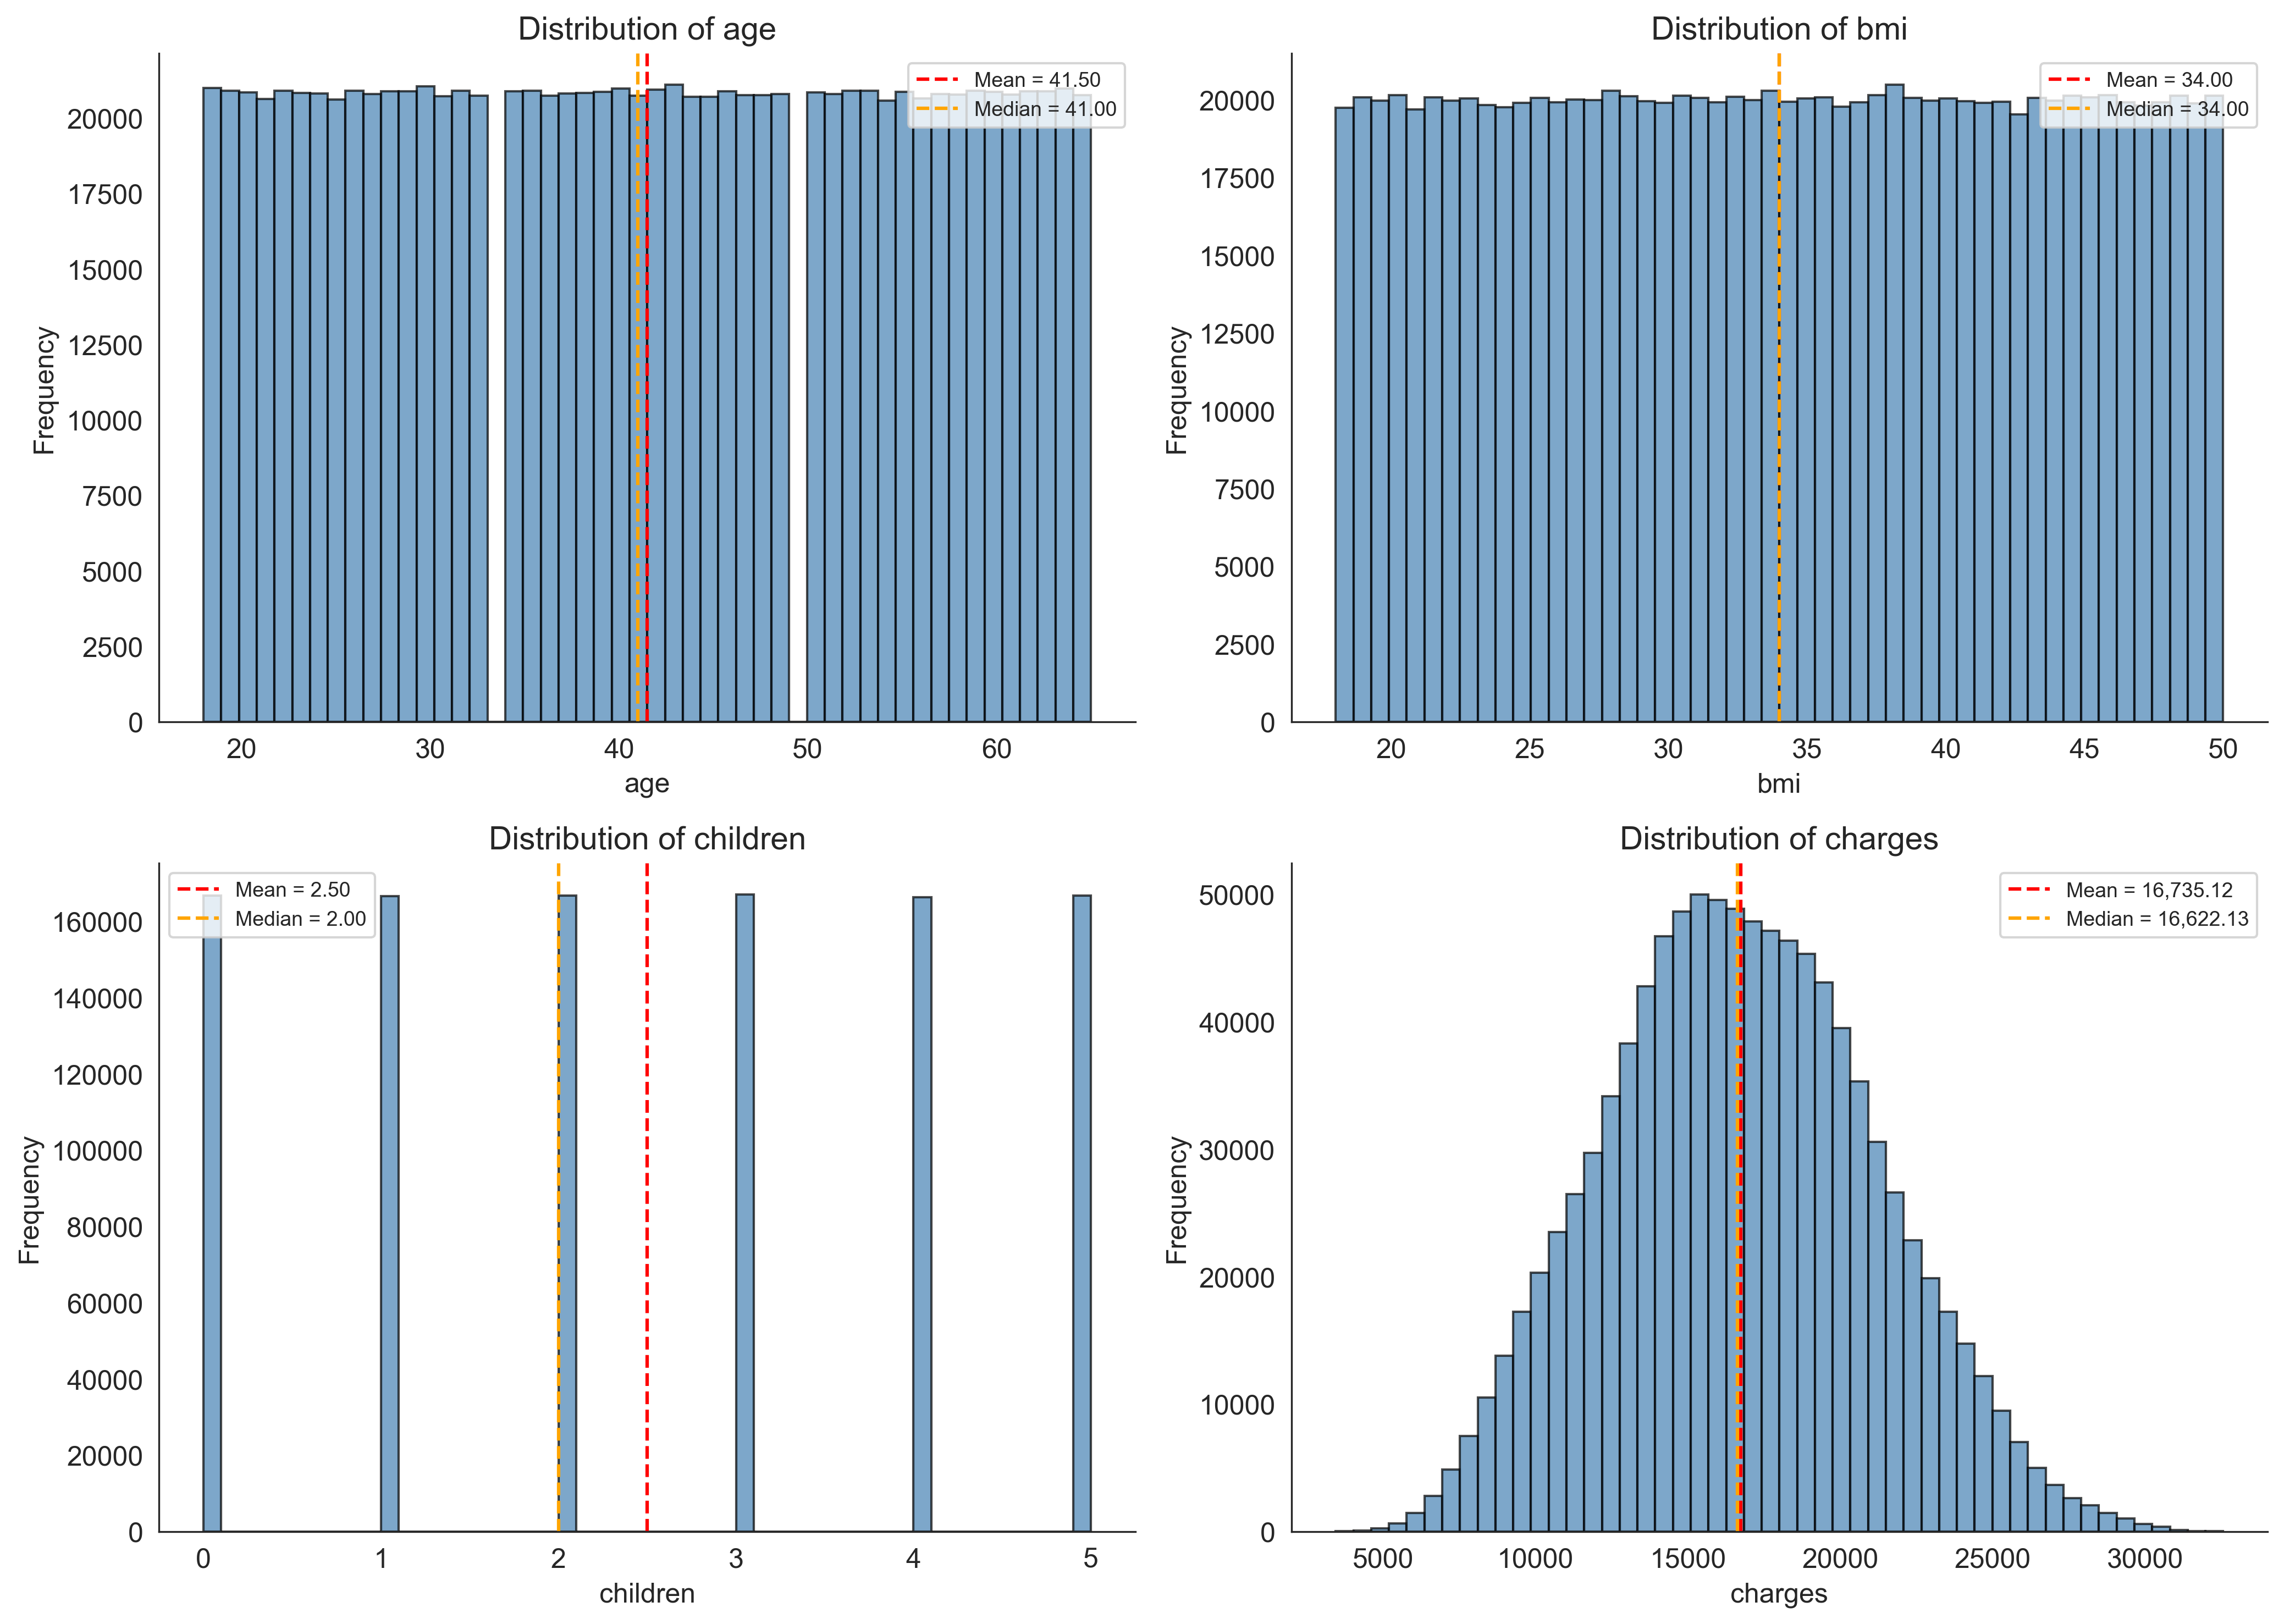
\includegraphics[width=0.90\textwidth]{Thesis/Chapter 3/Figures/fig_numeric_distributions.png}
\caption{Empirical distributions of the numerical variables.}
\label{fig:numeric_distributions}
\end{figure}

Selected percentiles of \texttt{charges} are reported in
Table~\ref{tab:charges_percentiles}.  The interquartile range is
approximately $6\,181$, and the 90th, 95th, and 99th percentiles are
$22\,591$, $24\,224$, and $27\,016$, respectively.  These values serve as
empirical scale references; in the later \gls{mc} and Shapley stages,
high-cost profiles are defined using upper-tail quantiles of the
simulated predicted-cost distribution, not directly from these observed
percentiles.

\begin{table}[H]
\centering
\small
\renewcommand{\arraystretch}{1.12}
\begin{tabular}{lrrrrrrrrr}
\toprule
\textbf{Percentile} & P1 & P5 & P10 & P25 & P50 & P75 & P90 & P95 & P99 \\
\midrule
\textbf{Value} &
7\,520 & 9\,558 & 10\,947 & 13\,600 & 16\,622 &
19\,781 & 22\,591 & 24\,224 & 27\,016 \\
\bottomrule
\end{tabular}
\caption{Selected percentiles of the response variable \texttt{charges}.}
\label{tab:charges_percentiles}
\end{table}

% ----------------------------
% 3.3.2 DEPENDENCE STRUCTURE
% ----------------------------

\subsubsection{Dependence structure}
The Pearson correlation matrix for the four numerical variables is given
in Table~\ref{tab:numeric_correlations}.

\begin{table}[H]
\centering
\small
\renewcommand{\arraystretch}{1.12}
\begin{tabular}{lrrrr}
\toprule
 & \texttt{age} & \texttt{bmi} & \texttt{children} & \texttt{charges} \\
\midrule
\texttt{age}      & 1.000 & 0.001 & $-0.001$ & 0.063 \\
\texttt{bmi}      & 0.001 & 1.000 & $-0.002$ & 0.104 \\
\texttt{children} & $-0.001$ & $-0.002$ & 1.000 & 0.077 \\
\texttt{charges}  & 0.063 & 0.104 & 0.077 & 1.000 \\
\bottomrule
\end{tabular}
\caption{Pearson correlation matrix for the numerical variables.}
\label{tab:numeric_correlations}
\end{table}

Pairwise correlations among the predictors are negligible
($|r| \le 0.002$), and the marginal correlations with \texttt{charges} are
weak.  This does not imply that the predictors are
unimportant (the deep
network can learn complex nonlinear interactions invisible to a linear
correlation matrix), but it does provide empirical support for the
product-marginal independence assumption used in the \gls{mc}
simulation.  The correlation heatmap in Figure~\ref{fig:correlation_heatmap}
confirms the uniformly pale off-diagonal shading.

\begin{figure}[H]
\centering
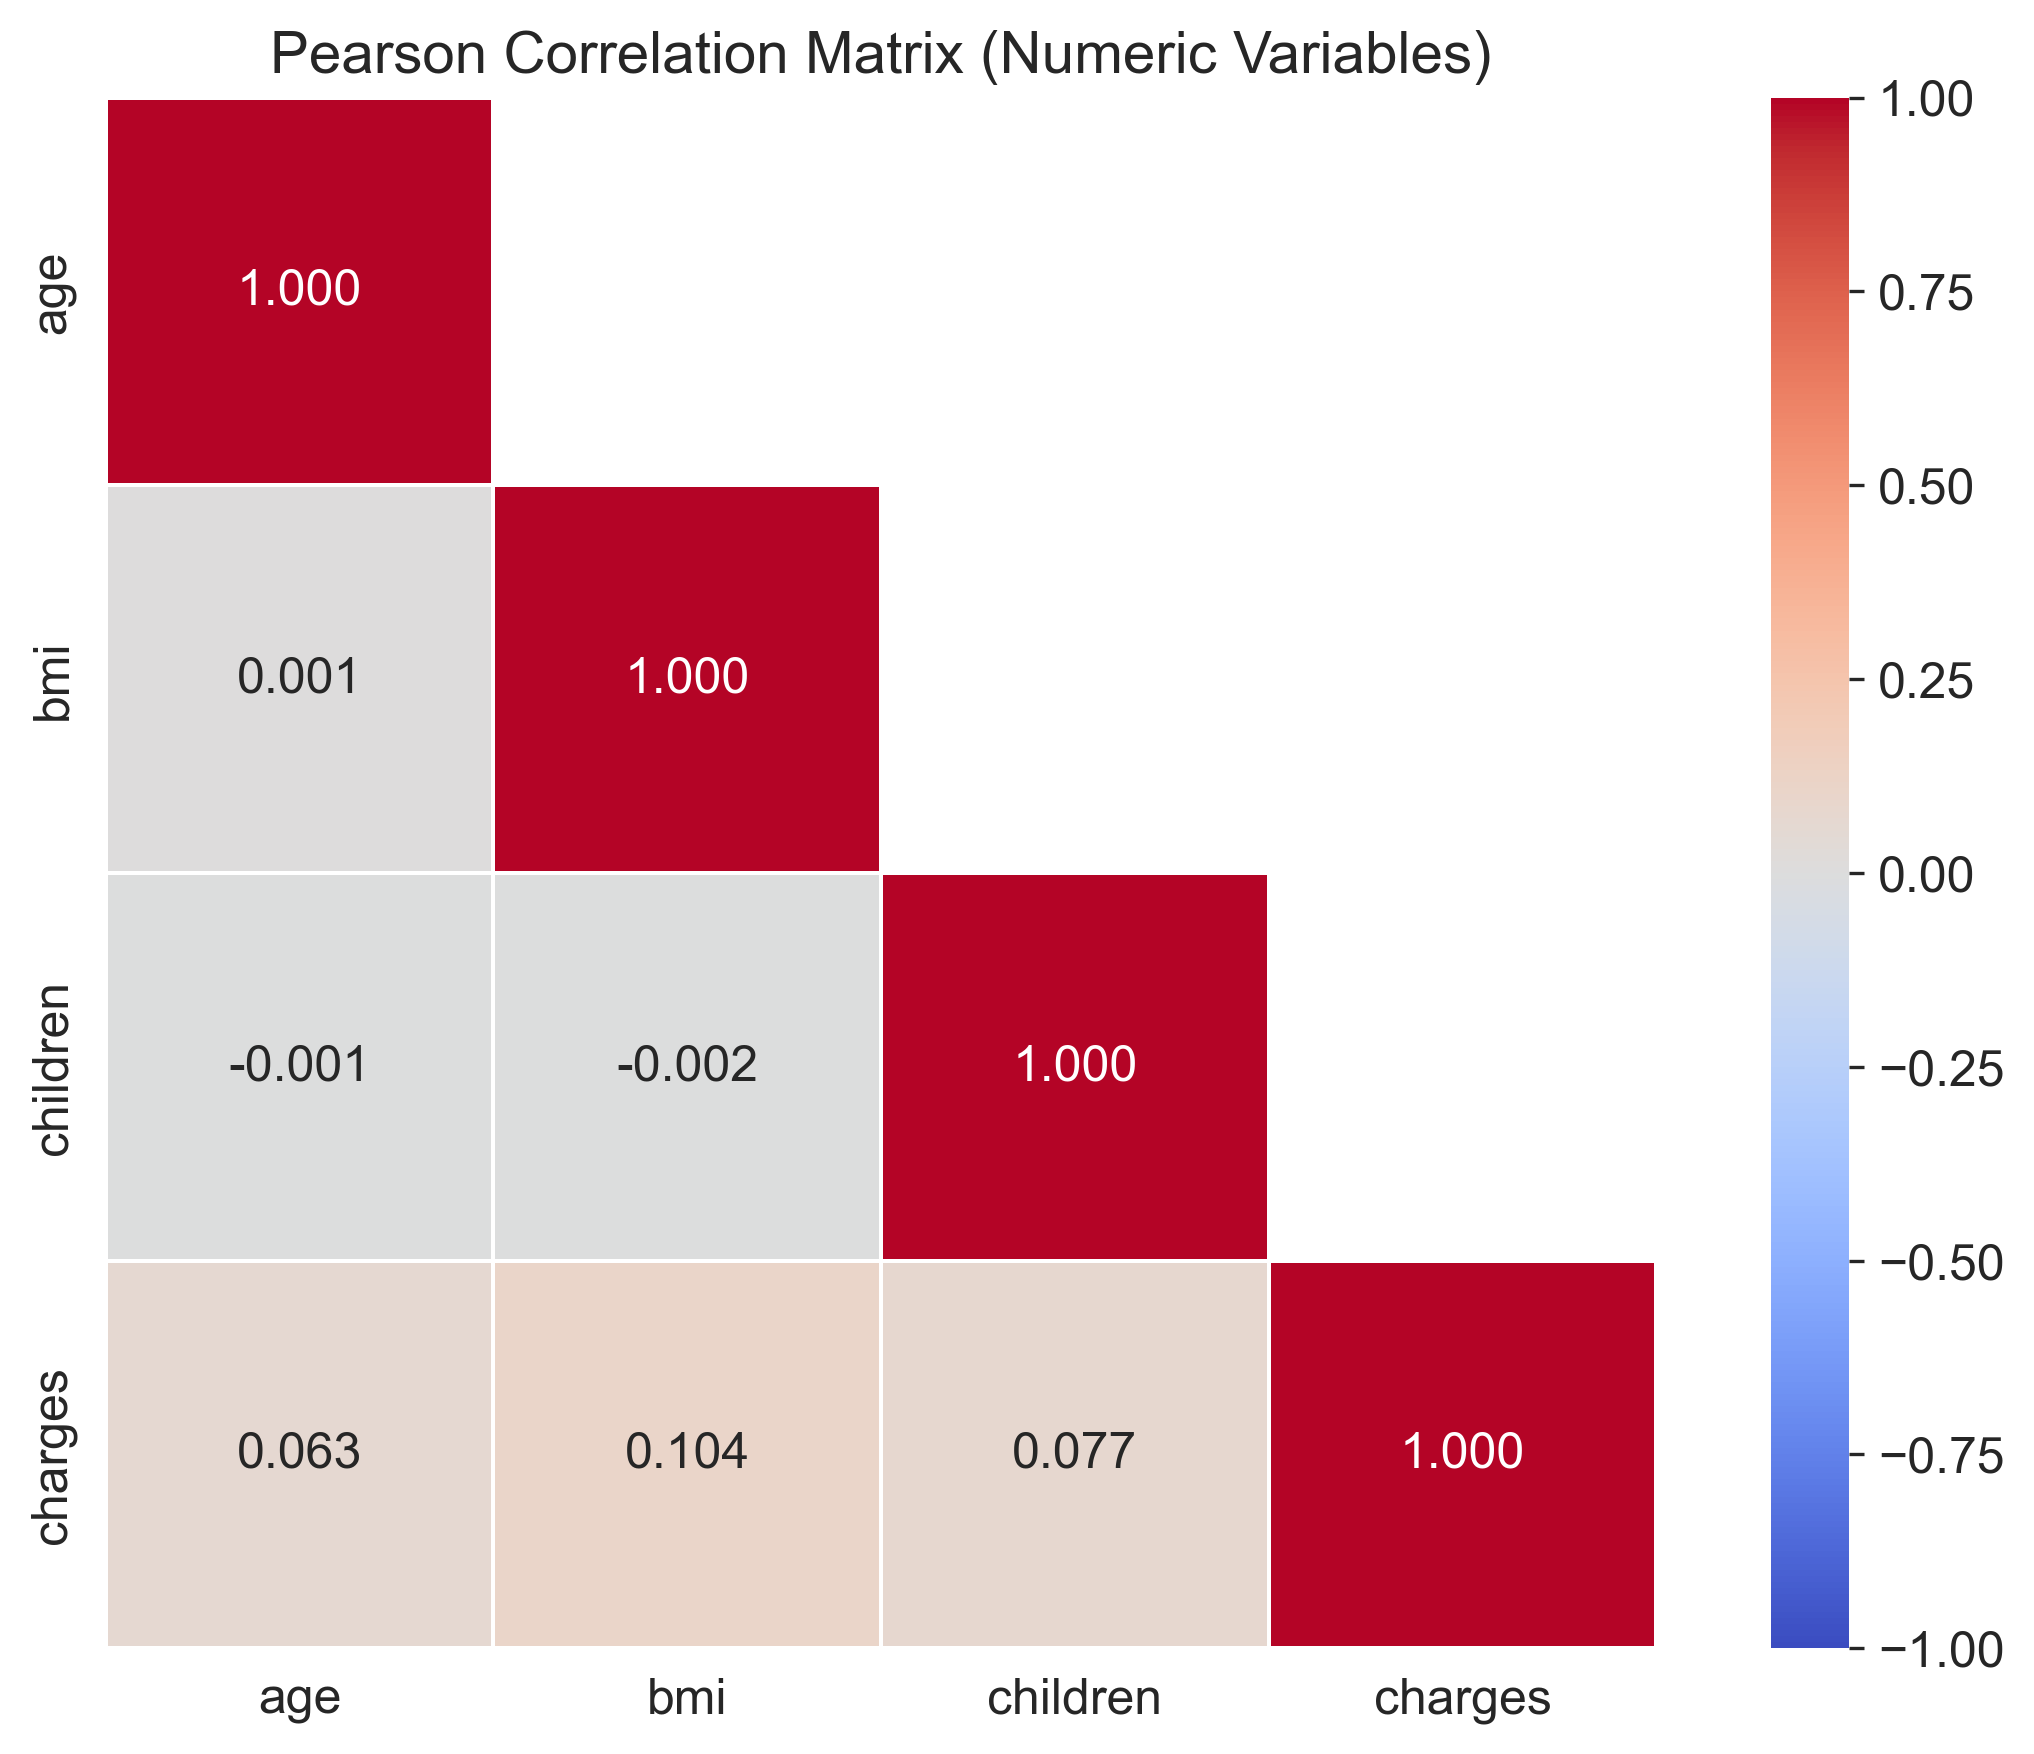
\includegraphics[width=0.60\textwidth]{Thesis/Chapter 3/Figures/fig_correlation_heatmap.png}
\caption{Pearson correlation heatmap for the numerical variables.}
\label{fig:correlation_heatmap}
\end{figure}

% ---------------------------------------------------
% 3.3.3 CATEGORICAL PREDICTORS AND ENCODED FEATURES
% ---------------------------------------------------

\subsubsection{Categorical predictors and encoded features}

\begin{figure}[H]
\centering
\begin{subfigure}[b]{\textwidth}
    \centering
    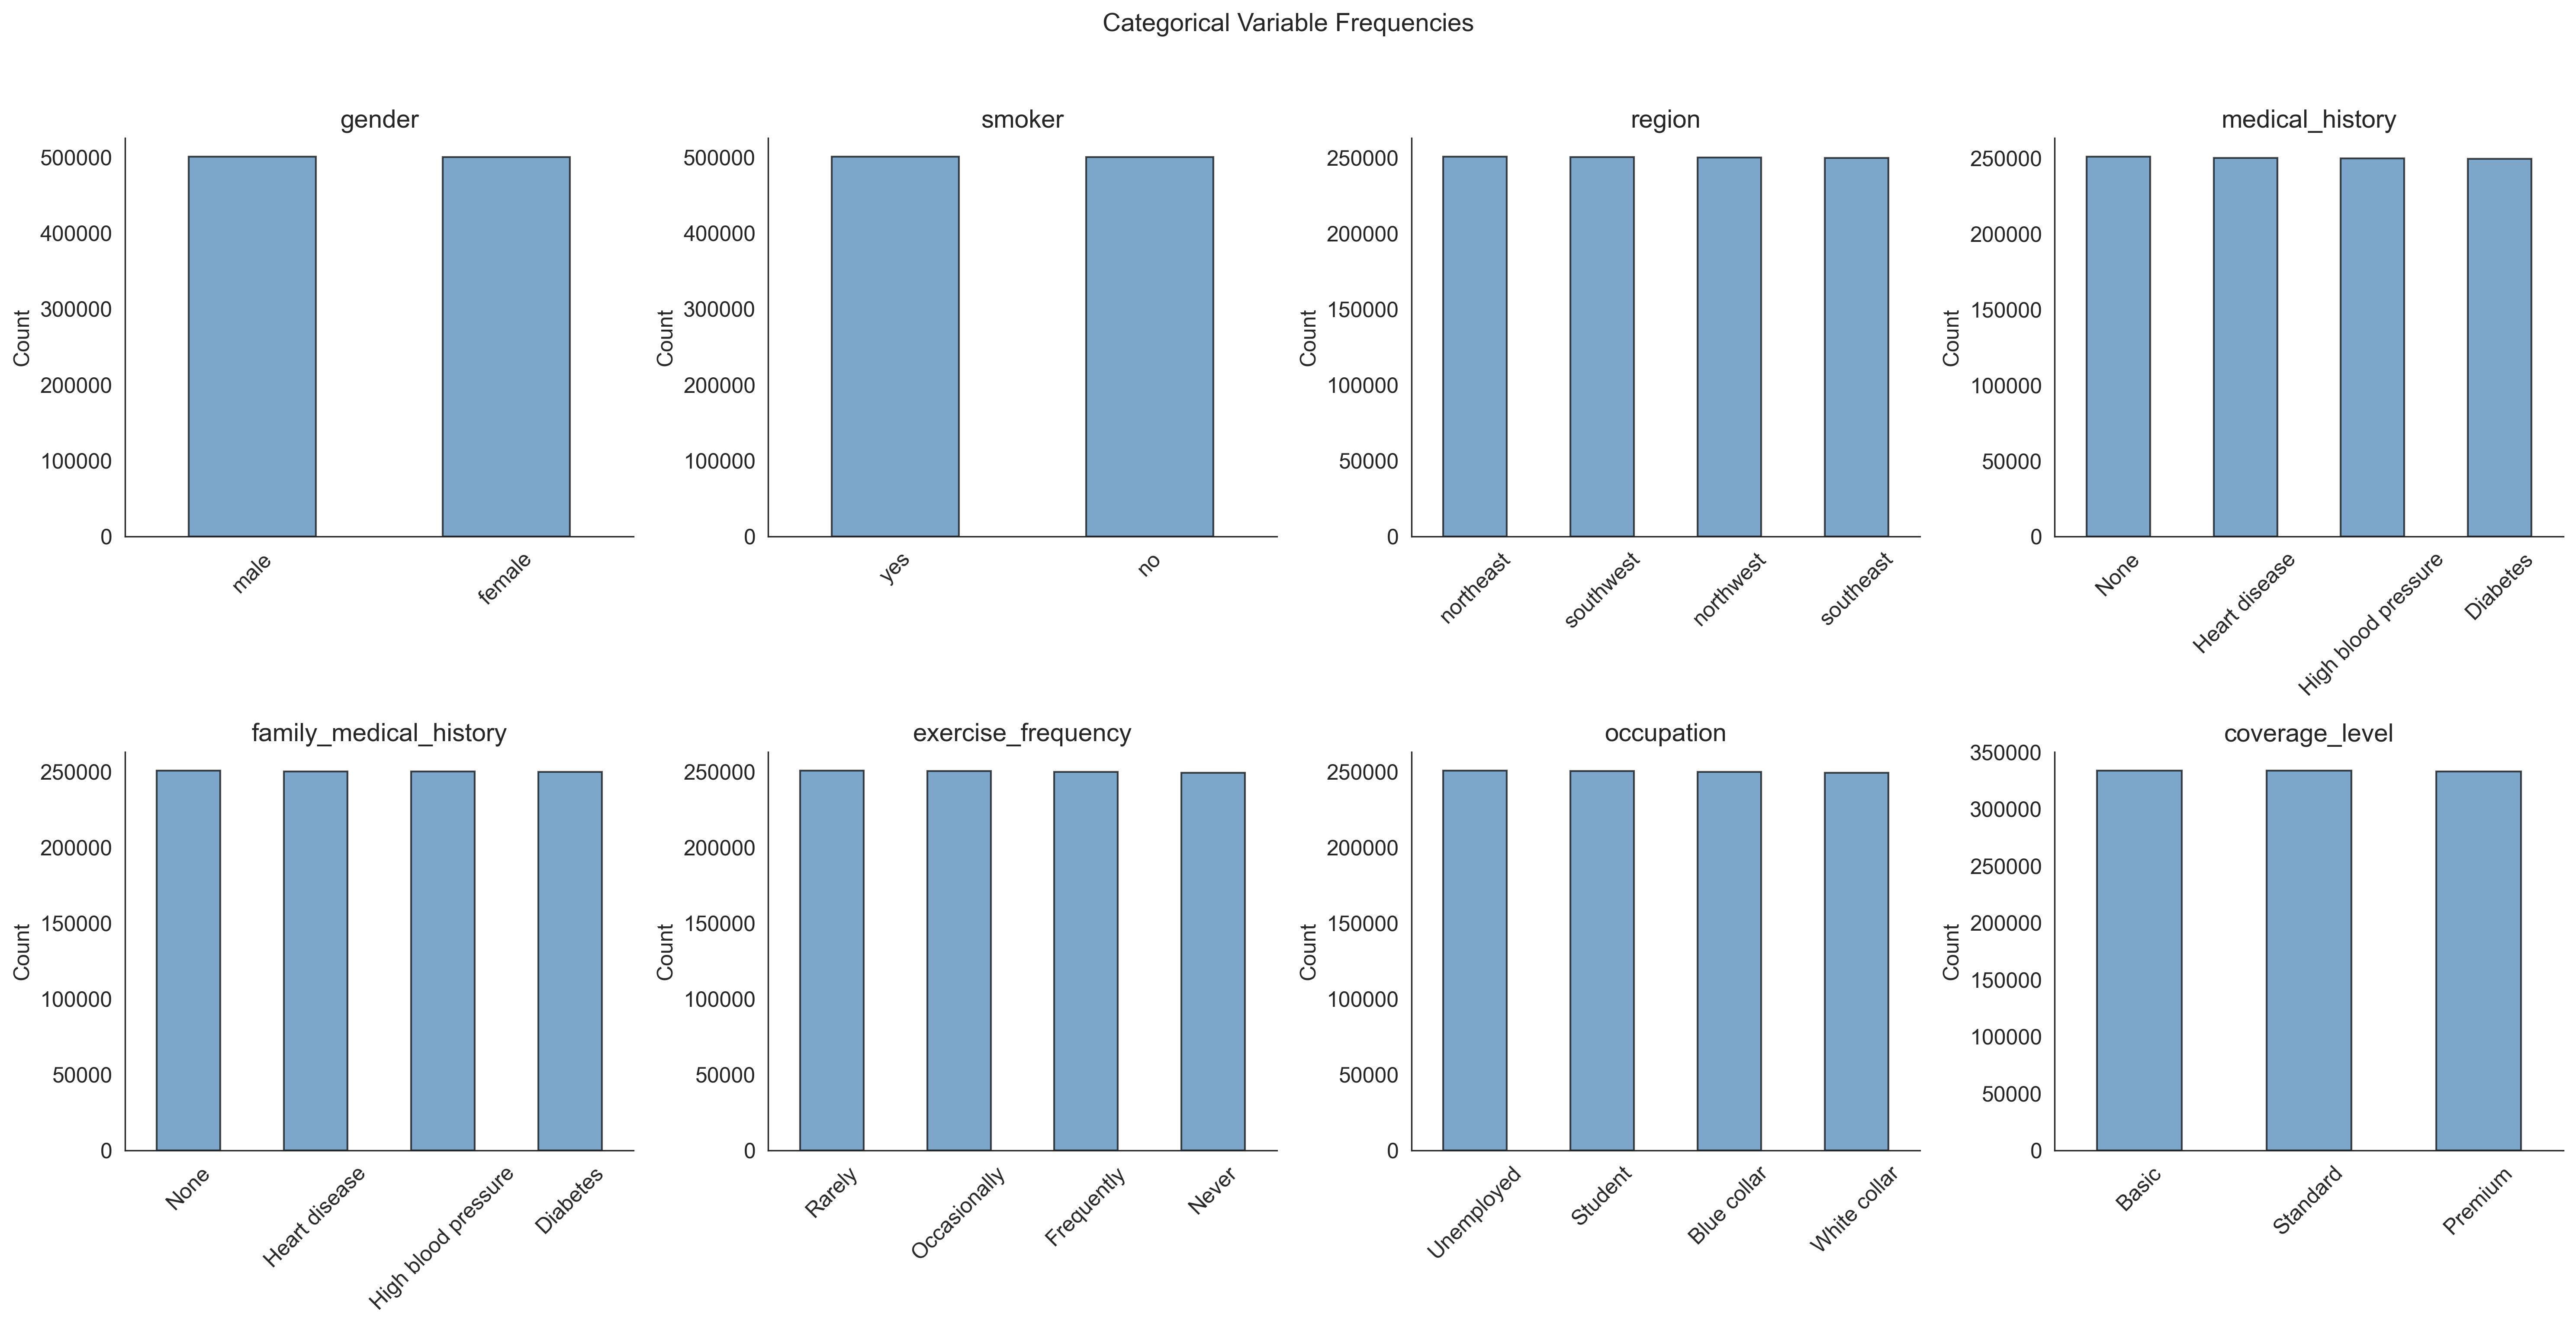
\includegraphics[width=0.95\textwidth]{Thesis/Chapter 3/Figures/fig_categorical_frequencies.png}
    \caption{Frequency distributions of categorical and binary predictors.}
    \label{fig:categorical_frequencies_ch3}
\end{subfigure}

\vspace{0.4cm}

\begin{subfigure}[b]{\textwidth}
    \centering
    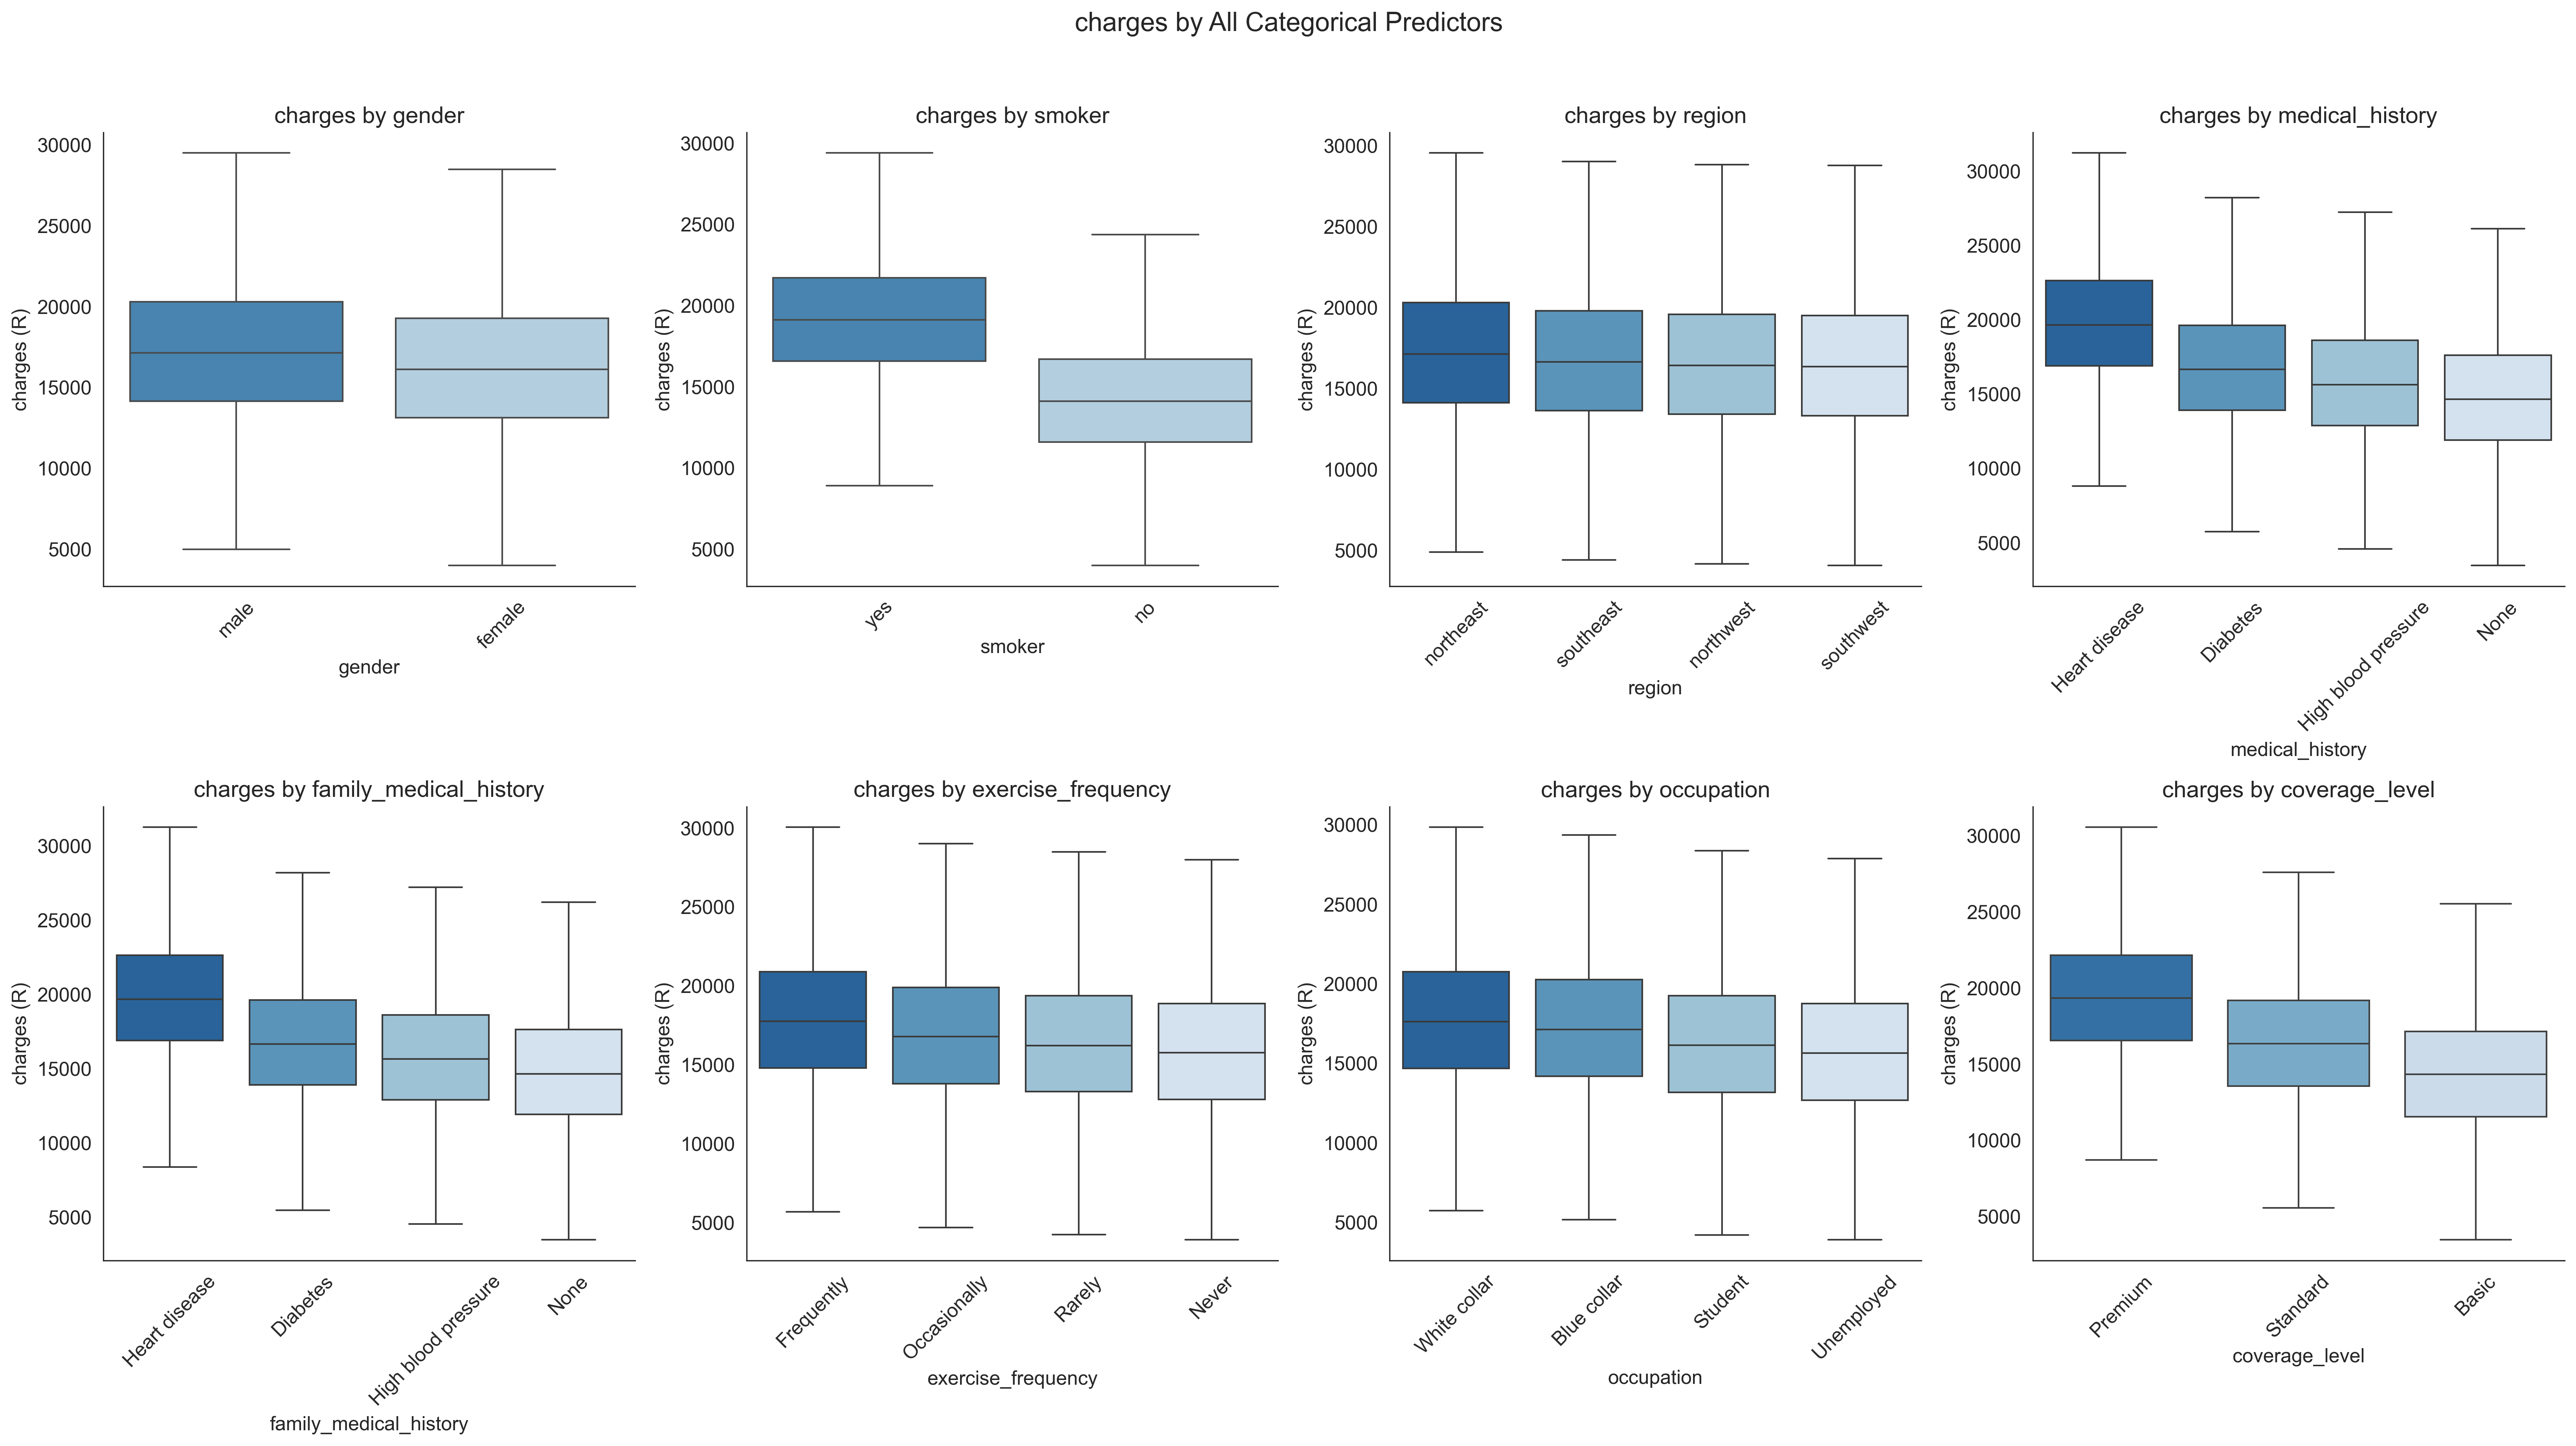
\includegraphics[width=0.95\textwidth]{Thesis/Chapter 3/Figures/fig_charges_by_all_categoricals.png}
    \caption{Boxplots of \texttt{charges} by categorical predictor.}
    \label{fig:charges_by_all_categoricals_ch3}
\end{subfigure}
\caption{Categorical predictor diagnostics: frequency distributions and conditional boxplots.}
\label{fig:categorical_diagnostics_ch3}
\end{figure}

\noindent
Figure~\ref{fig:categorical_frequencies_ch3} confirms that every
categorical and binary predictor is approximately uniformly distributed
across its levels. The two binary variables (\texttt{gender} and
\texttt{smoker}) each have close to 500\,000 observations per level, the
four-level variables (\texttt{region},\allowbreak{}
\texttt{medical\_\allowbreak{}history},\allowbreak{}
\texttt{family\_medical\_\allowbreak{}history},\allowbreak{}
\texttt{exercise\_\allowbreak{}frequency} and
\texttt{occupation}) each have approximately 250\,000 observations per
level, and the three-level \texttt{coverage\_\allowbreak{}level} variable has
approximately 333\,000 observations per tier. These balanced frequencies
ensure that no category is underrepresented in the training data and that
the fitted category proportions used in the \gls{mc} simulation are
estimated with high precision.

Figure~\ref{fig:charges_by_all_categoricals_ch3} displays the conditional
distribution of charges for each categorical predictor. The
\texttt{smoker} panel shows the clearest separation: smokers have a median
near R19\,000 compared to approximately R14\,000 for non-smokers. The
\texttt{coverage\_\allowbreak{}level} panel reveals a monotonic tier structure, with
Premium policyholders having the highest median charges (approximately
R20\,000), followed by Standard (approximately R17\,000) and Basic
(approximately R15\,000). Among \texttt{medical\_\allowbreak{}history} categories,
Heart disease is associated with the highest median charges (approximately
R20\,000), followed by Diabetes, High blood pressure and None. The
\texttt{family\_medical\_\allowbreak{}history} panel shows the same ordering, with Heart
disease again yielding the highest charges. The \texttt{exercise\_\allowbreak{}frequency}
panel shows a modest gradient, with Frequently exercising policyholders
having marginally higher median charges than those who Never exercise.
The \texttt{gender}, \texttt{region} and \texttt{occupation} panels display
smaller unconditional differences, though males tend to have slightly
higher charges than females across all panels.

Two-way interactions were examined for
\texttt{smoker}~$\times$~\texttt{coverage\_\allowbreak{}level},
\texttt{smoker}~$\times$~\texttt{medical\_\allowbreak{}history} and
\texttt{coverage\_\allowbreak{}level}~$\times$~\texttt{gender} to assess whether the
effect of one variable on charges depends on the level of another.

\begin{figure}[H]
\centering
\begin{subfigure}[b]{\textwidth}
    \centering
    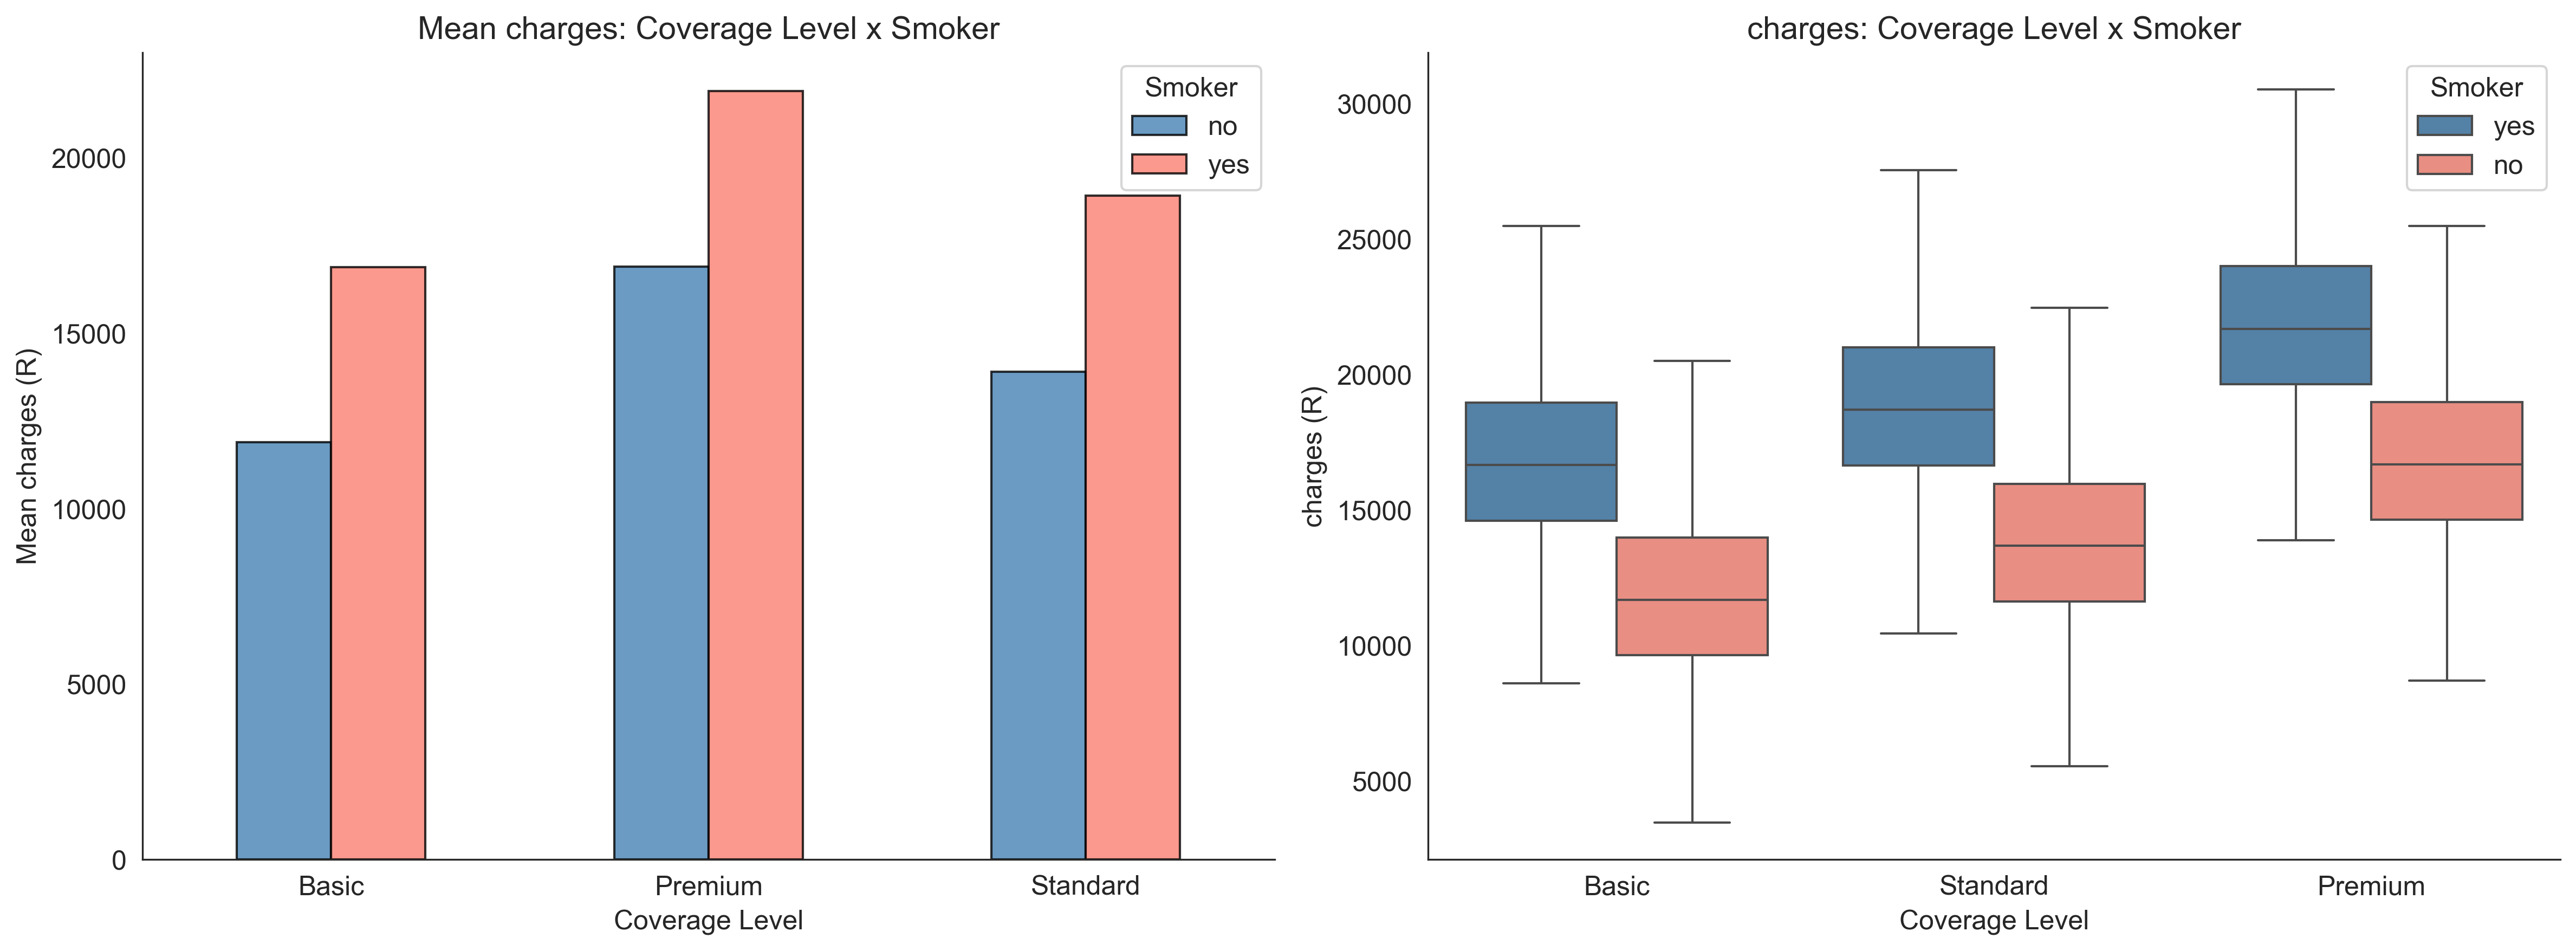
\includegraphics[width=0.95\textwidth]{Thesis/Chapter 3/Figures/fig_interaction_smoker_coverage.png}
    \caption{\texttt{smoker}~$\times$~\texttt{coverage\_\allowbreak{}level} interaction effects on charges.}
    \label{fig:interaction_smoker_coverage_ch3}
\end{subfigure}

\vspace{0.3cm}

\begin{subfigure}[b]{\textwidth}
    \centering
    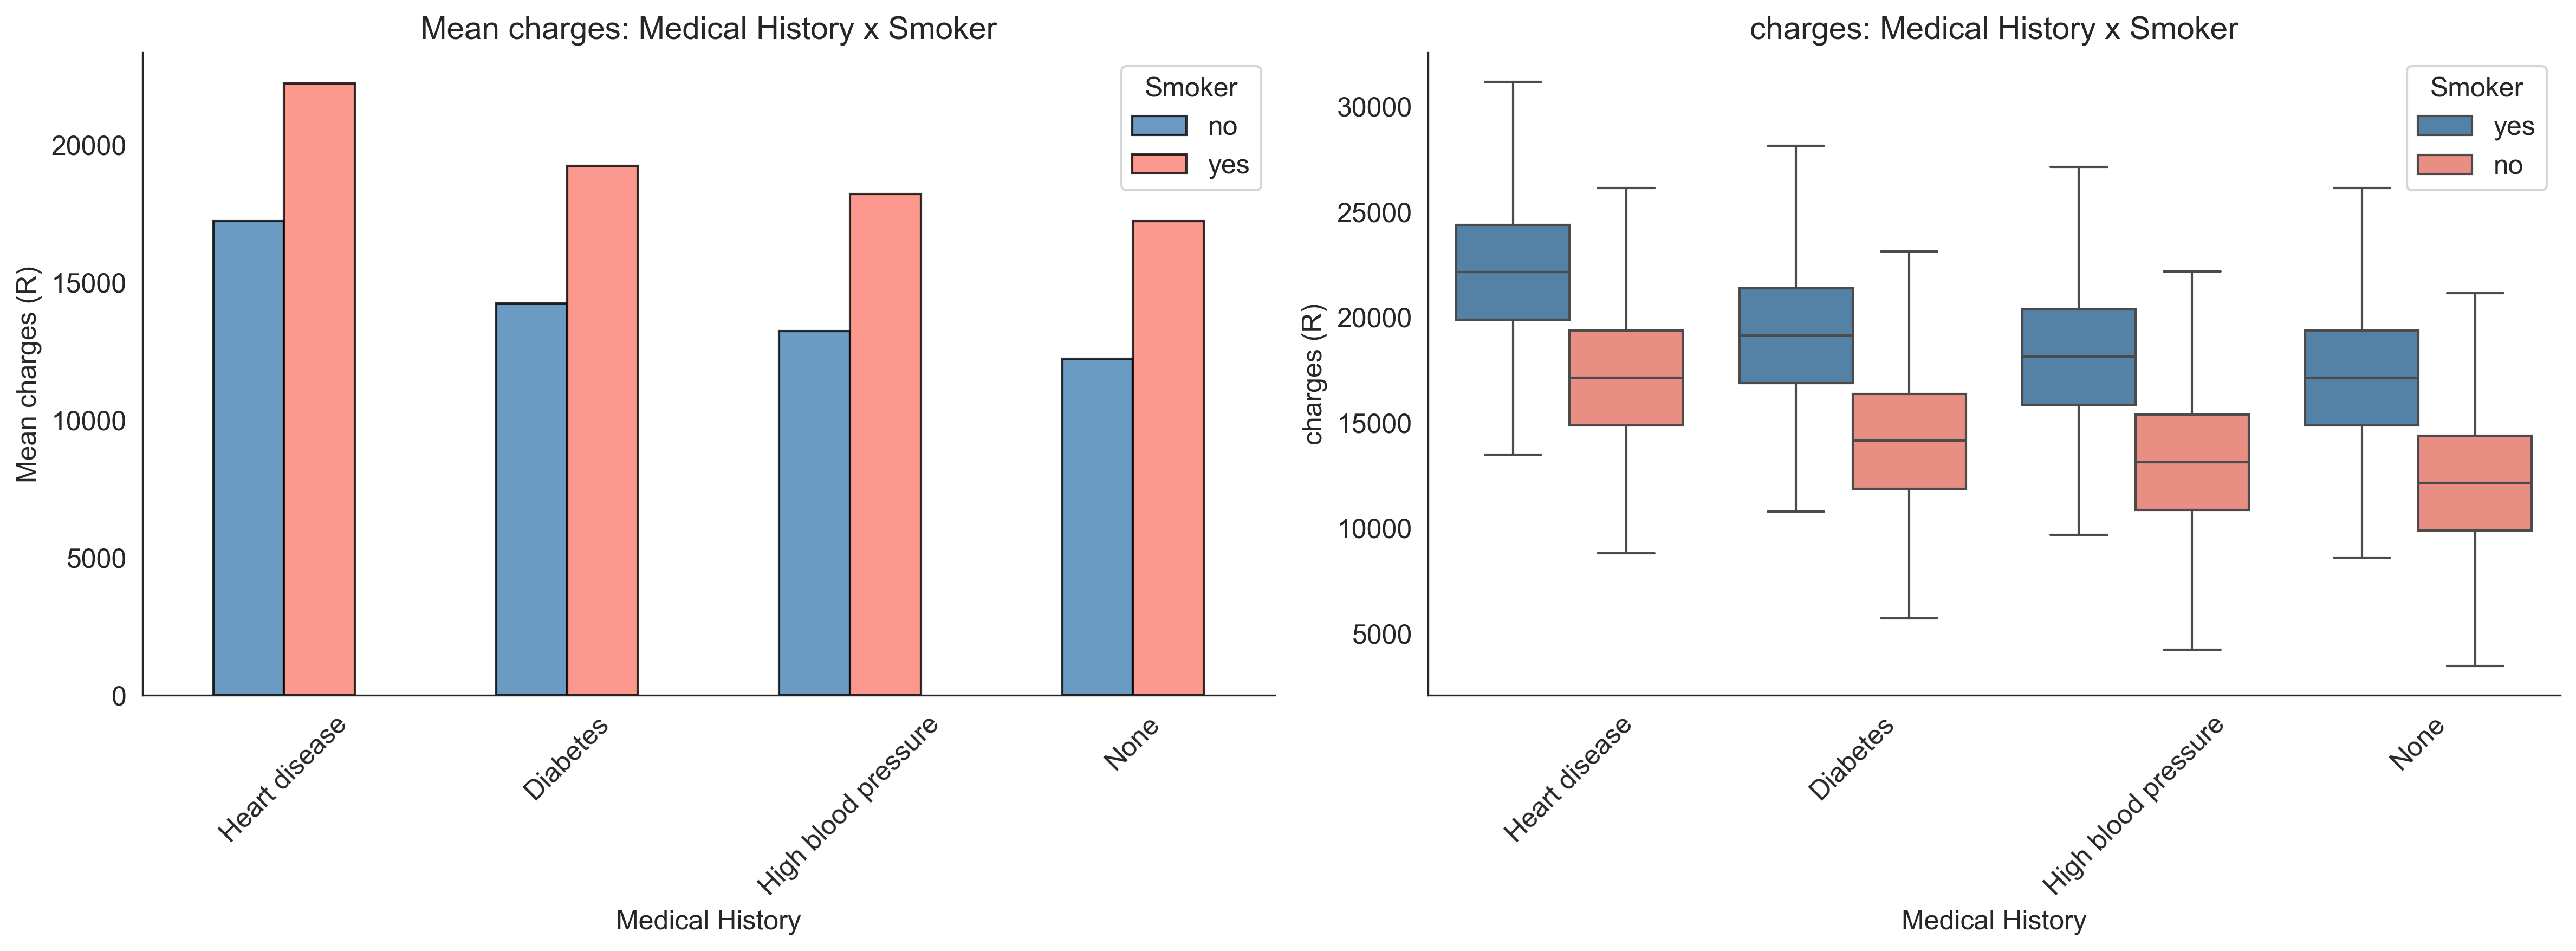
\includegraphics[width=0.95\textwidth]{Thesis/Chapter 3/Figures/fig_interaction_smoker_medical.png}
    \caption{\texttt{smoker}~$\times$~\texttt{medical\_\allowbreak{}history} interaction effects on charges.}
    \label{fig:interaction_smoker_medical_ch3}
\end{subfigure}

\vspace{0.3cm}

\begin{subfigure}[b]{0.65\textwidth}
    \centering
    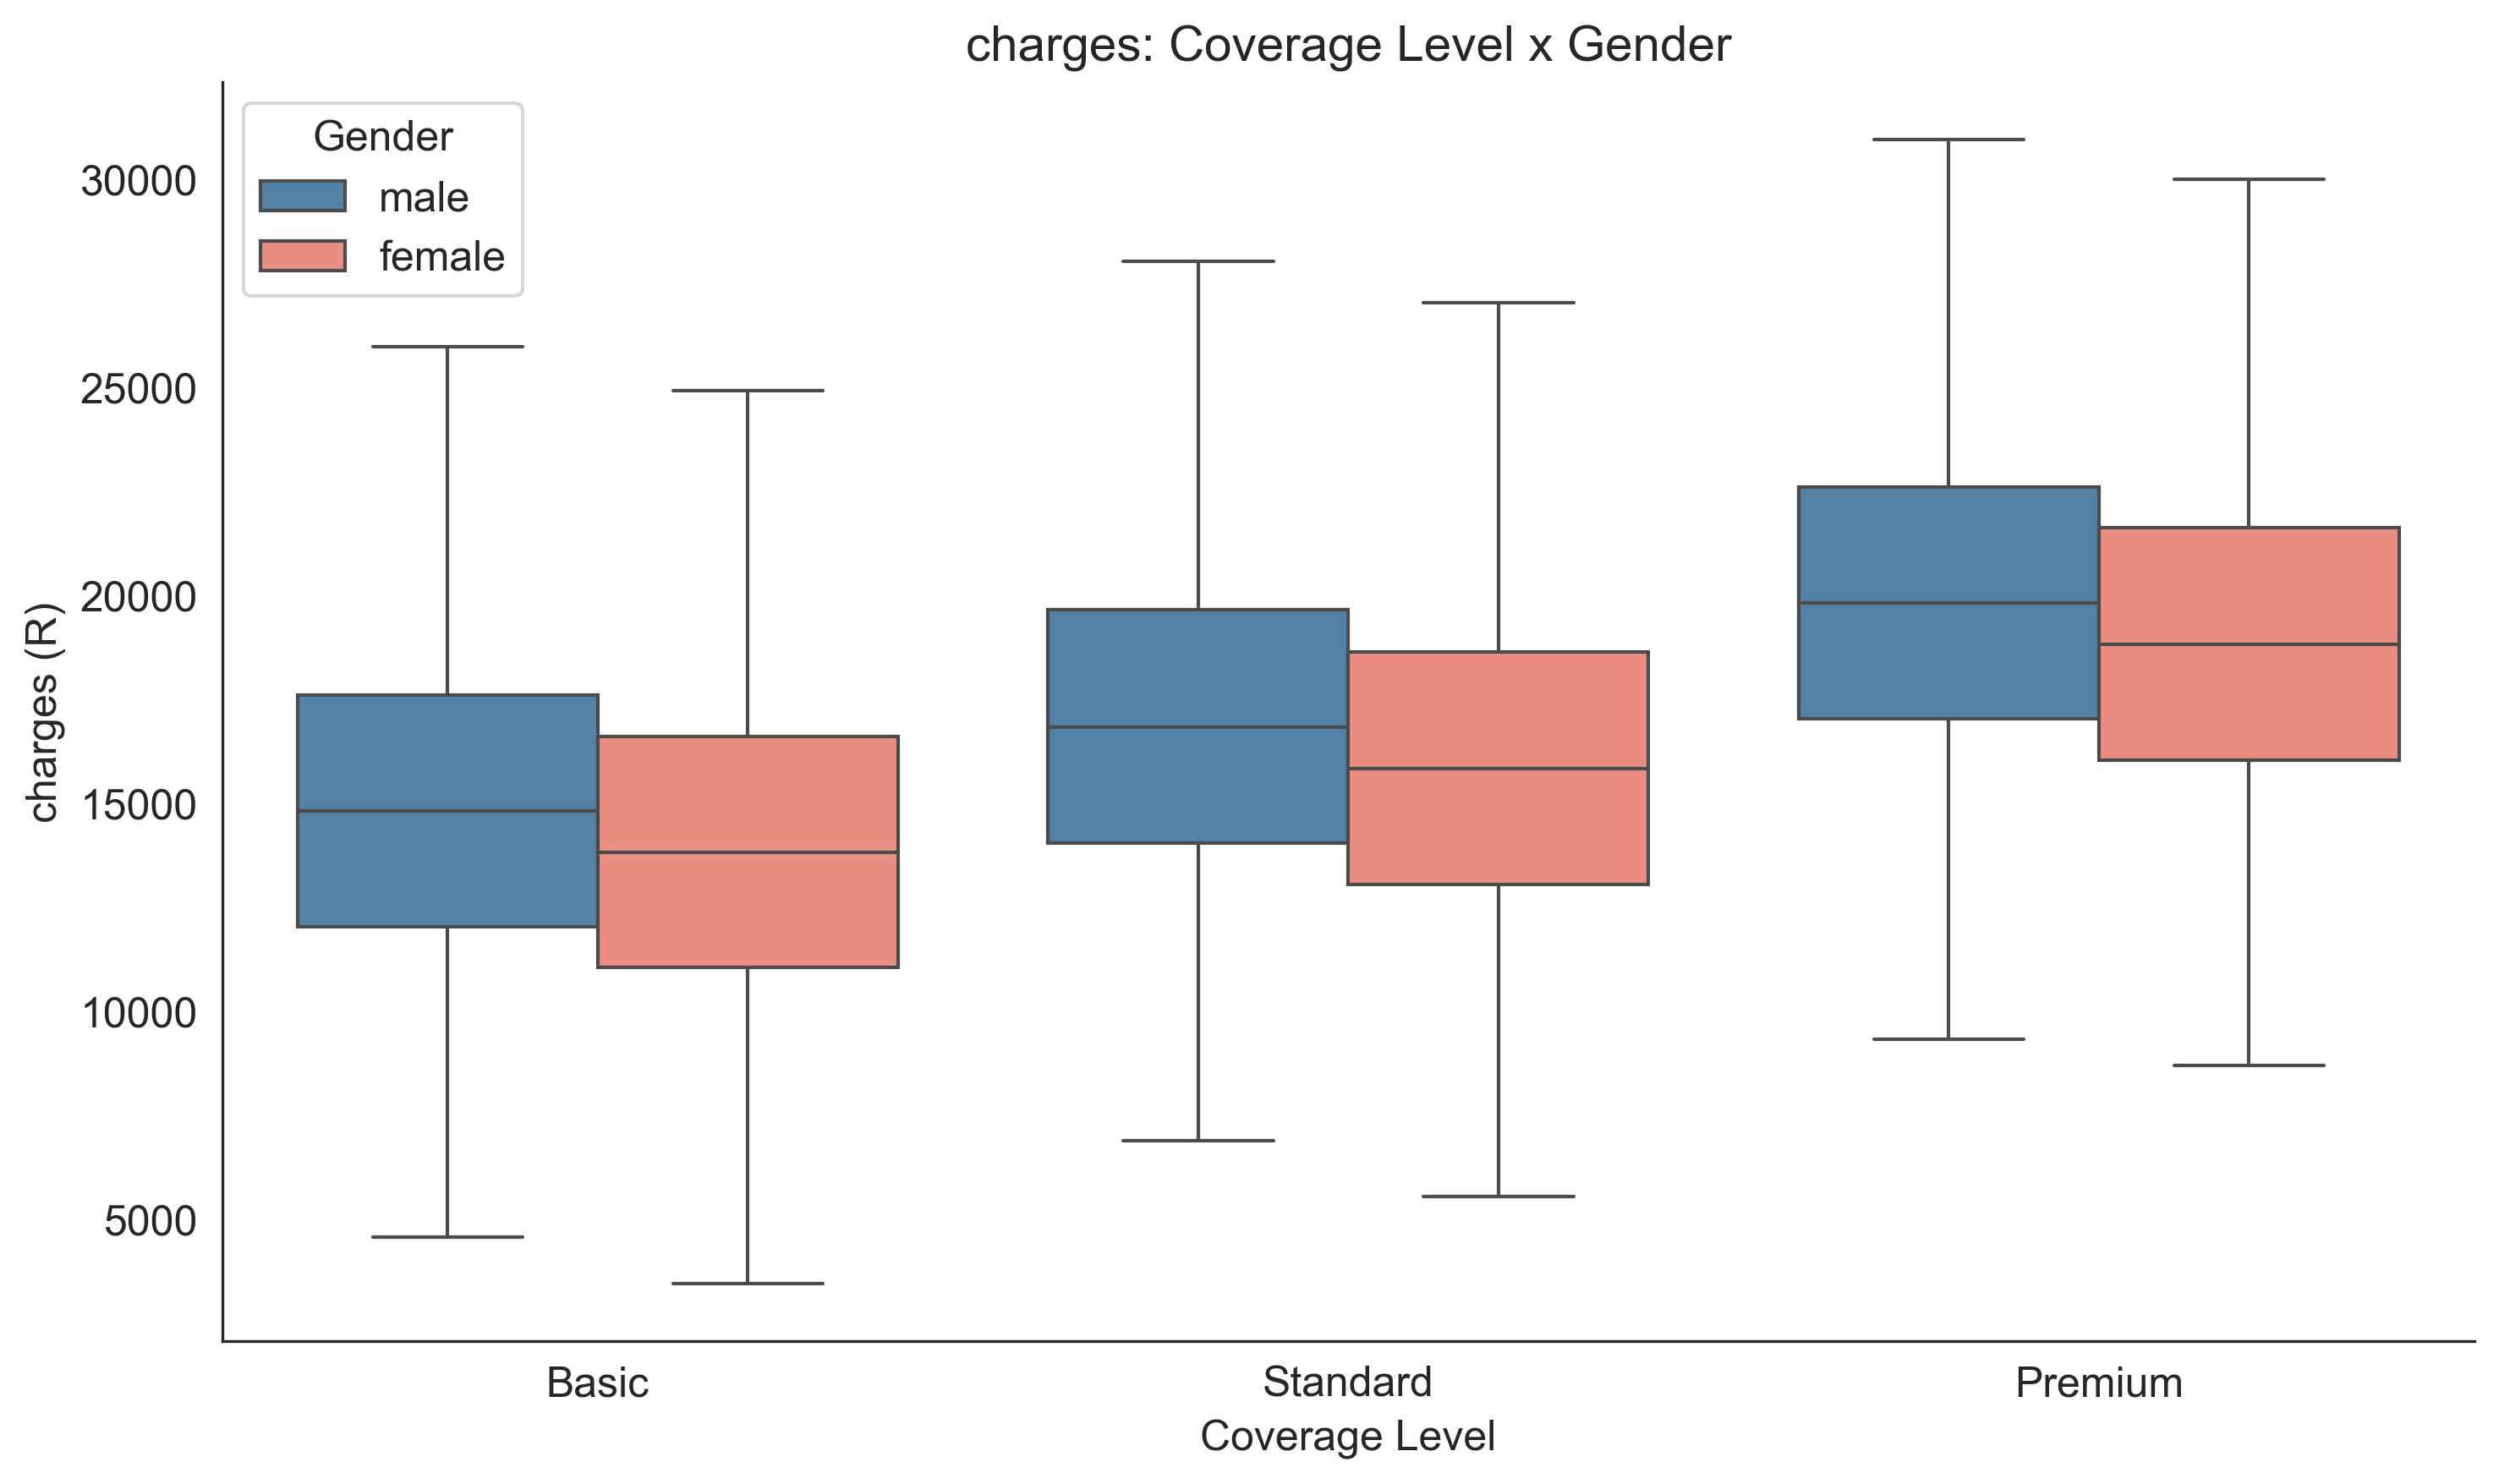
\includegraphics[width=\textwidth]{Thesis/Chapter 3/Figures/fig_interaction_coverage_gender.png}
    \caption{\texttt{coverage\_\allowbreak{}level}~$\times$~\texttt{gender} interaction effects on charges.}
    \label{fig:interaction_coverage_gender_ch3}
\end{subfigure}
\caption{Two-way interaction effects on \texttt{charges}.}
\label{fig:interaction_effects_ch3}
\end{figure}

\noindent
Figure~\ref{fig:interaction_smoker_coverage_ch3} shows that the smoker
effect is present at every coverage tier but is amplified at higher
coverage levels. At the Basic tier, the difference in mean charges between
smokers and non-smokers is approximately R5\,000 (R17\,000 versus R12\,000), whereas
at the Premium tier the difference widens to approximately R5\,000 to R6\,000
on a higher base (R22\,000 versus R17\,000). The boxplots confirm that
smokers consistently occupy a higher distributional range within each tier.
Figure~\ref{fig:interaction_smoker_medical_ch3} reveals a consistent
smoker premium across all medical history categories. The largest combined
effect occurs for smokers with Heart disease (mean charges approximately
R22\,500), while the lowest occurs for non-smokers with no reported
condition (approximately R12\,500). The smoker effect (approximately
R5\,000) is additive with the medical history effect, with the gap
remaining relatively stable across all four levels.
Figure~\ref{fig:interaction_coverage_gender_ch3} shows that males have
slightly higher median charges than females at every coverage tier, with
the gender gap widening modestly from Basic (approximately R1\,000) to
Premium (approximately R1\,500). The interaction effects visible in
Figure~\ref{fig:interaction_effects_ch3} support the use of a flexible \gls{dnn}
architecture capable of capturing nonlinear and interaction-based
relationships.

After encoding, the Pearson correlations between the 22 encoded predictors
and \texttt{charges} were computed on the training partition. The strongest
linear associations are \texttt{smoker} ($r = 0.567$),\allowbreak{}
\texttt{coverage\_level\_\allowbreak{}Premium} ($r = 0.427$),\allowbreak{}
\texttt{medical\_history\_\allowbreak{}Heart\_disease} ($r = 0.393$) and
\texttt{family\_medical\_\allowbreak{}history\_\allowbreak{}Heart\_disease} ($r = 0.393$).

\begin{figure}[H]
\centering
\begin{subfigure}[b]{0.48\textwidth}
    \centering
    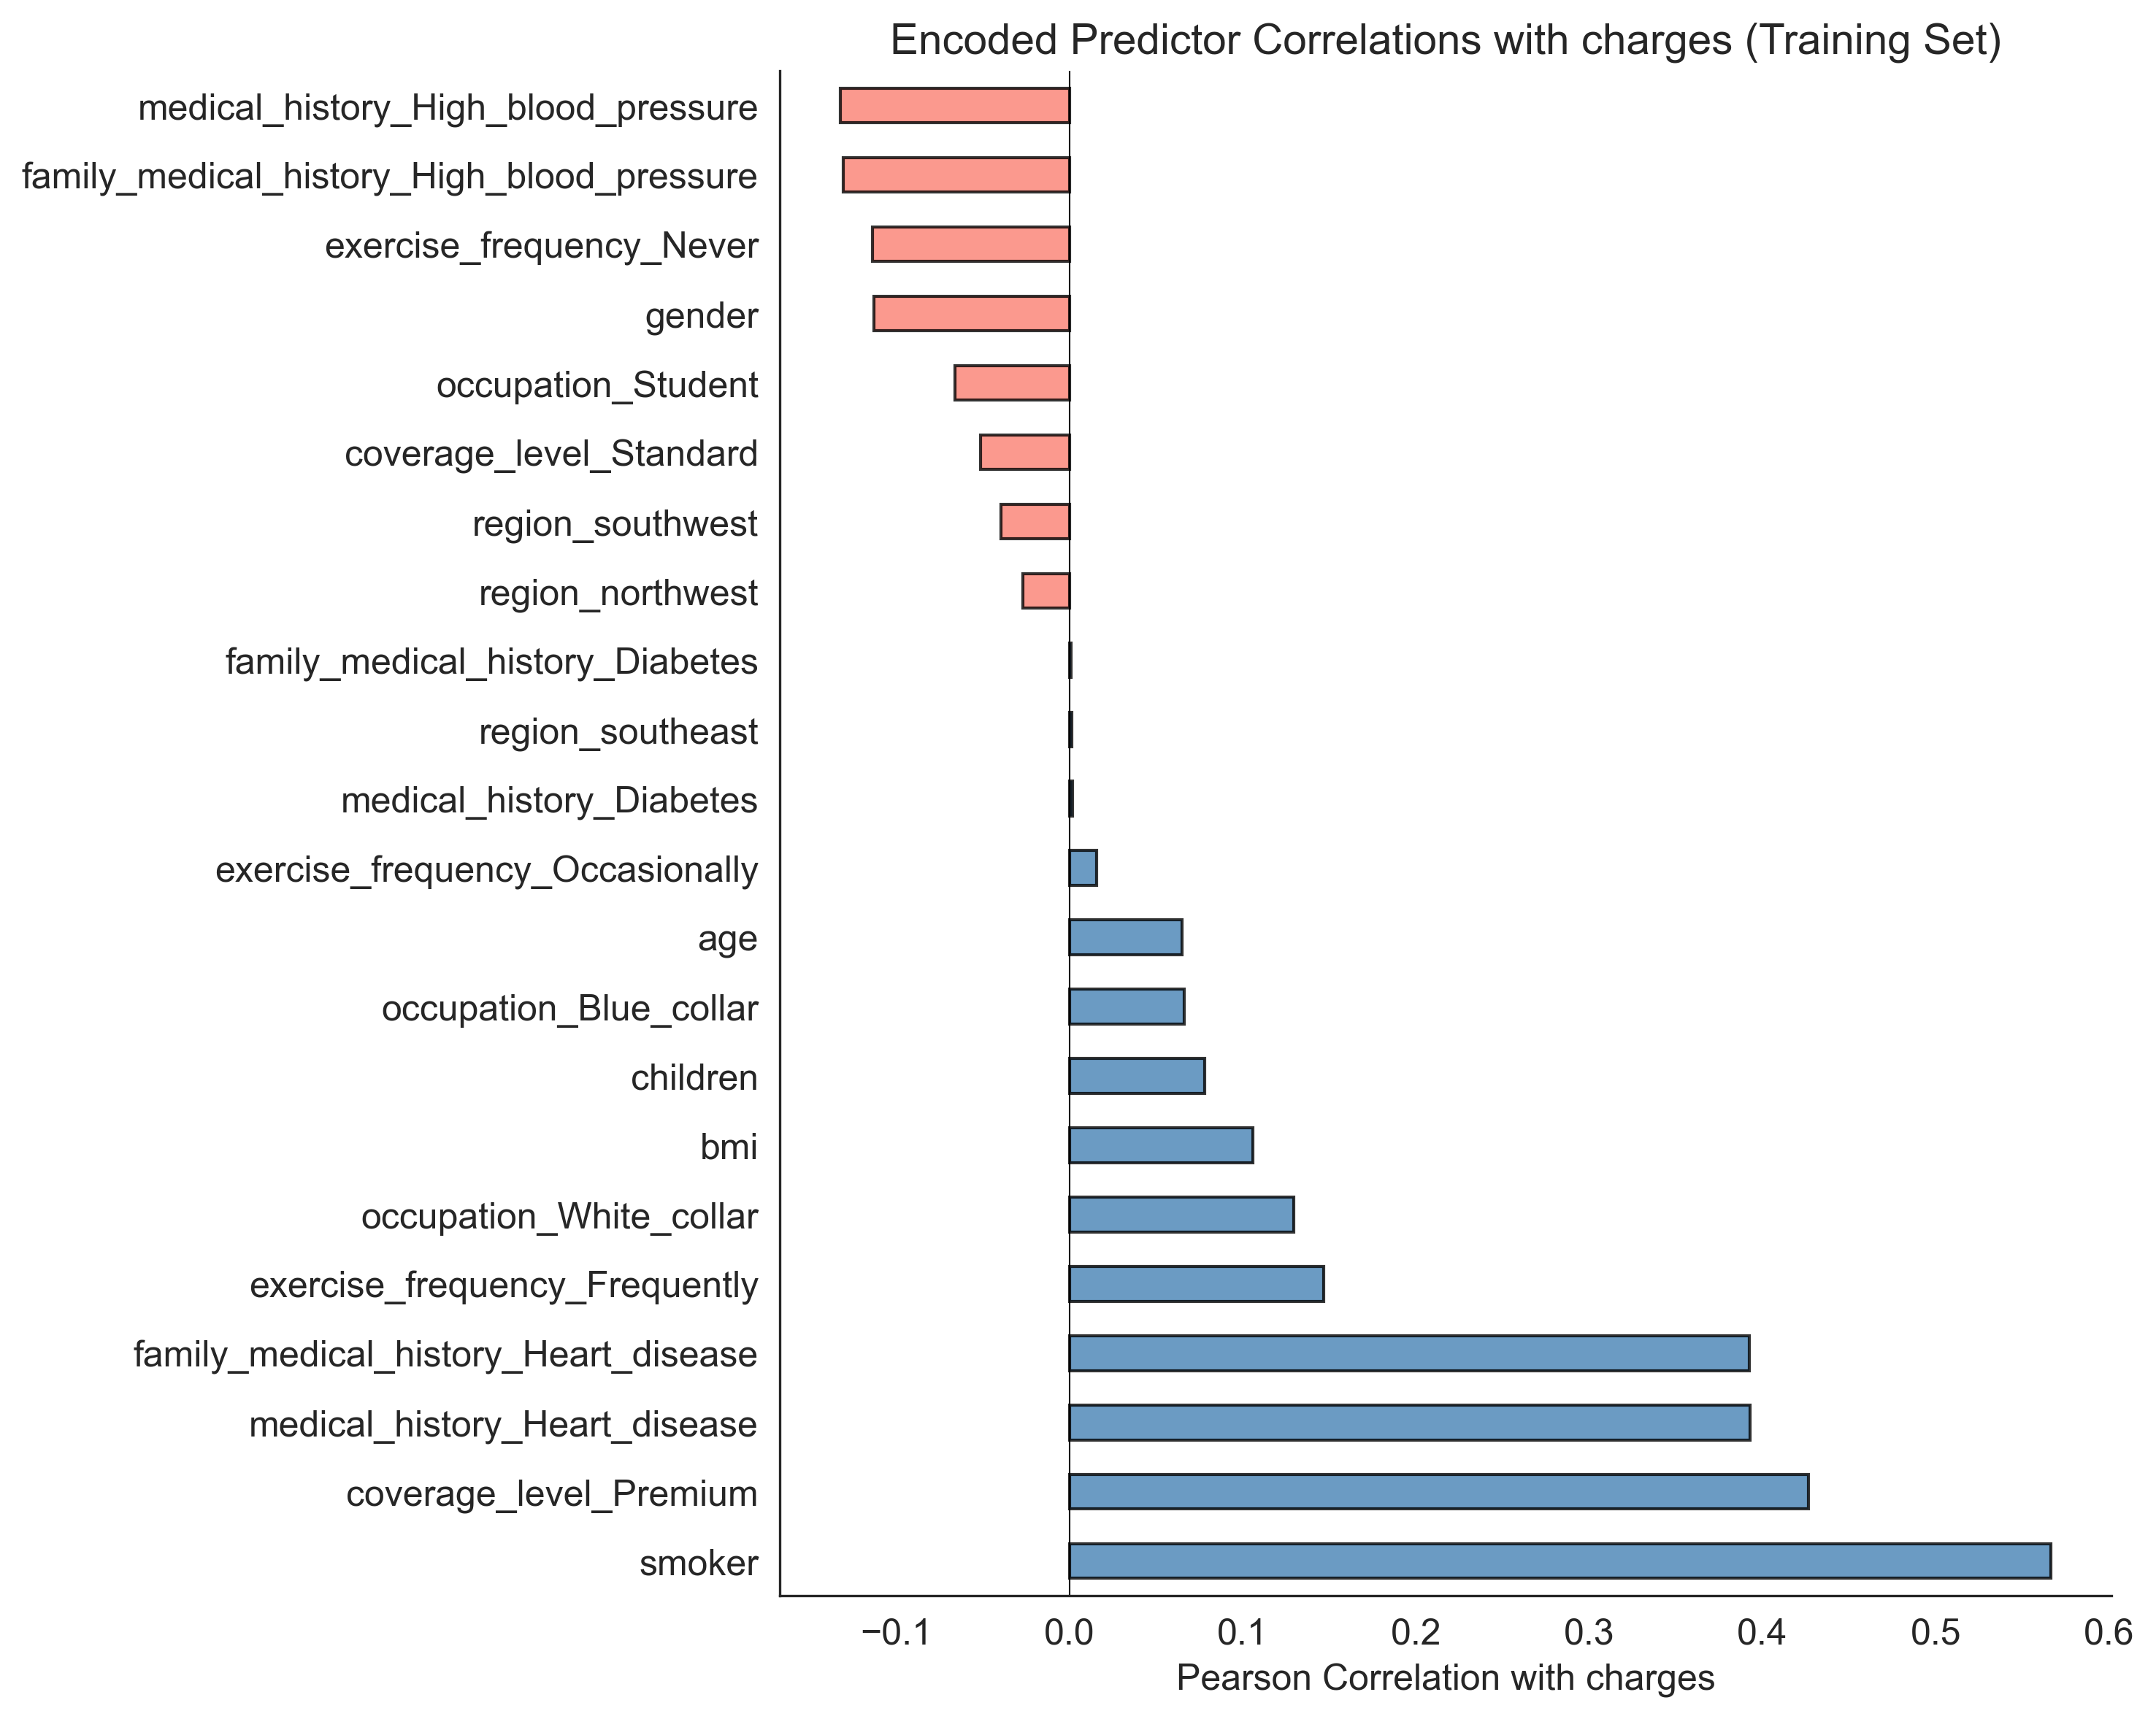
\includegraphics[width=\textwidth]{Thesis/Chapter 3/Figures/fig_encoded_correlations.png}
    \caption{Pearson correlations of encoded predictors with \texttt{charges}.}
    \label{fig:encoded_correlations_ch3}
\end{subfigure}
\hfill
\begin{subfigure}[b]{0.48\textwidth}
    \centering
    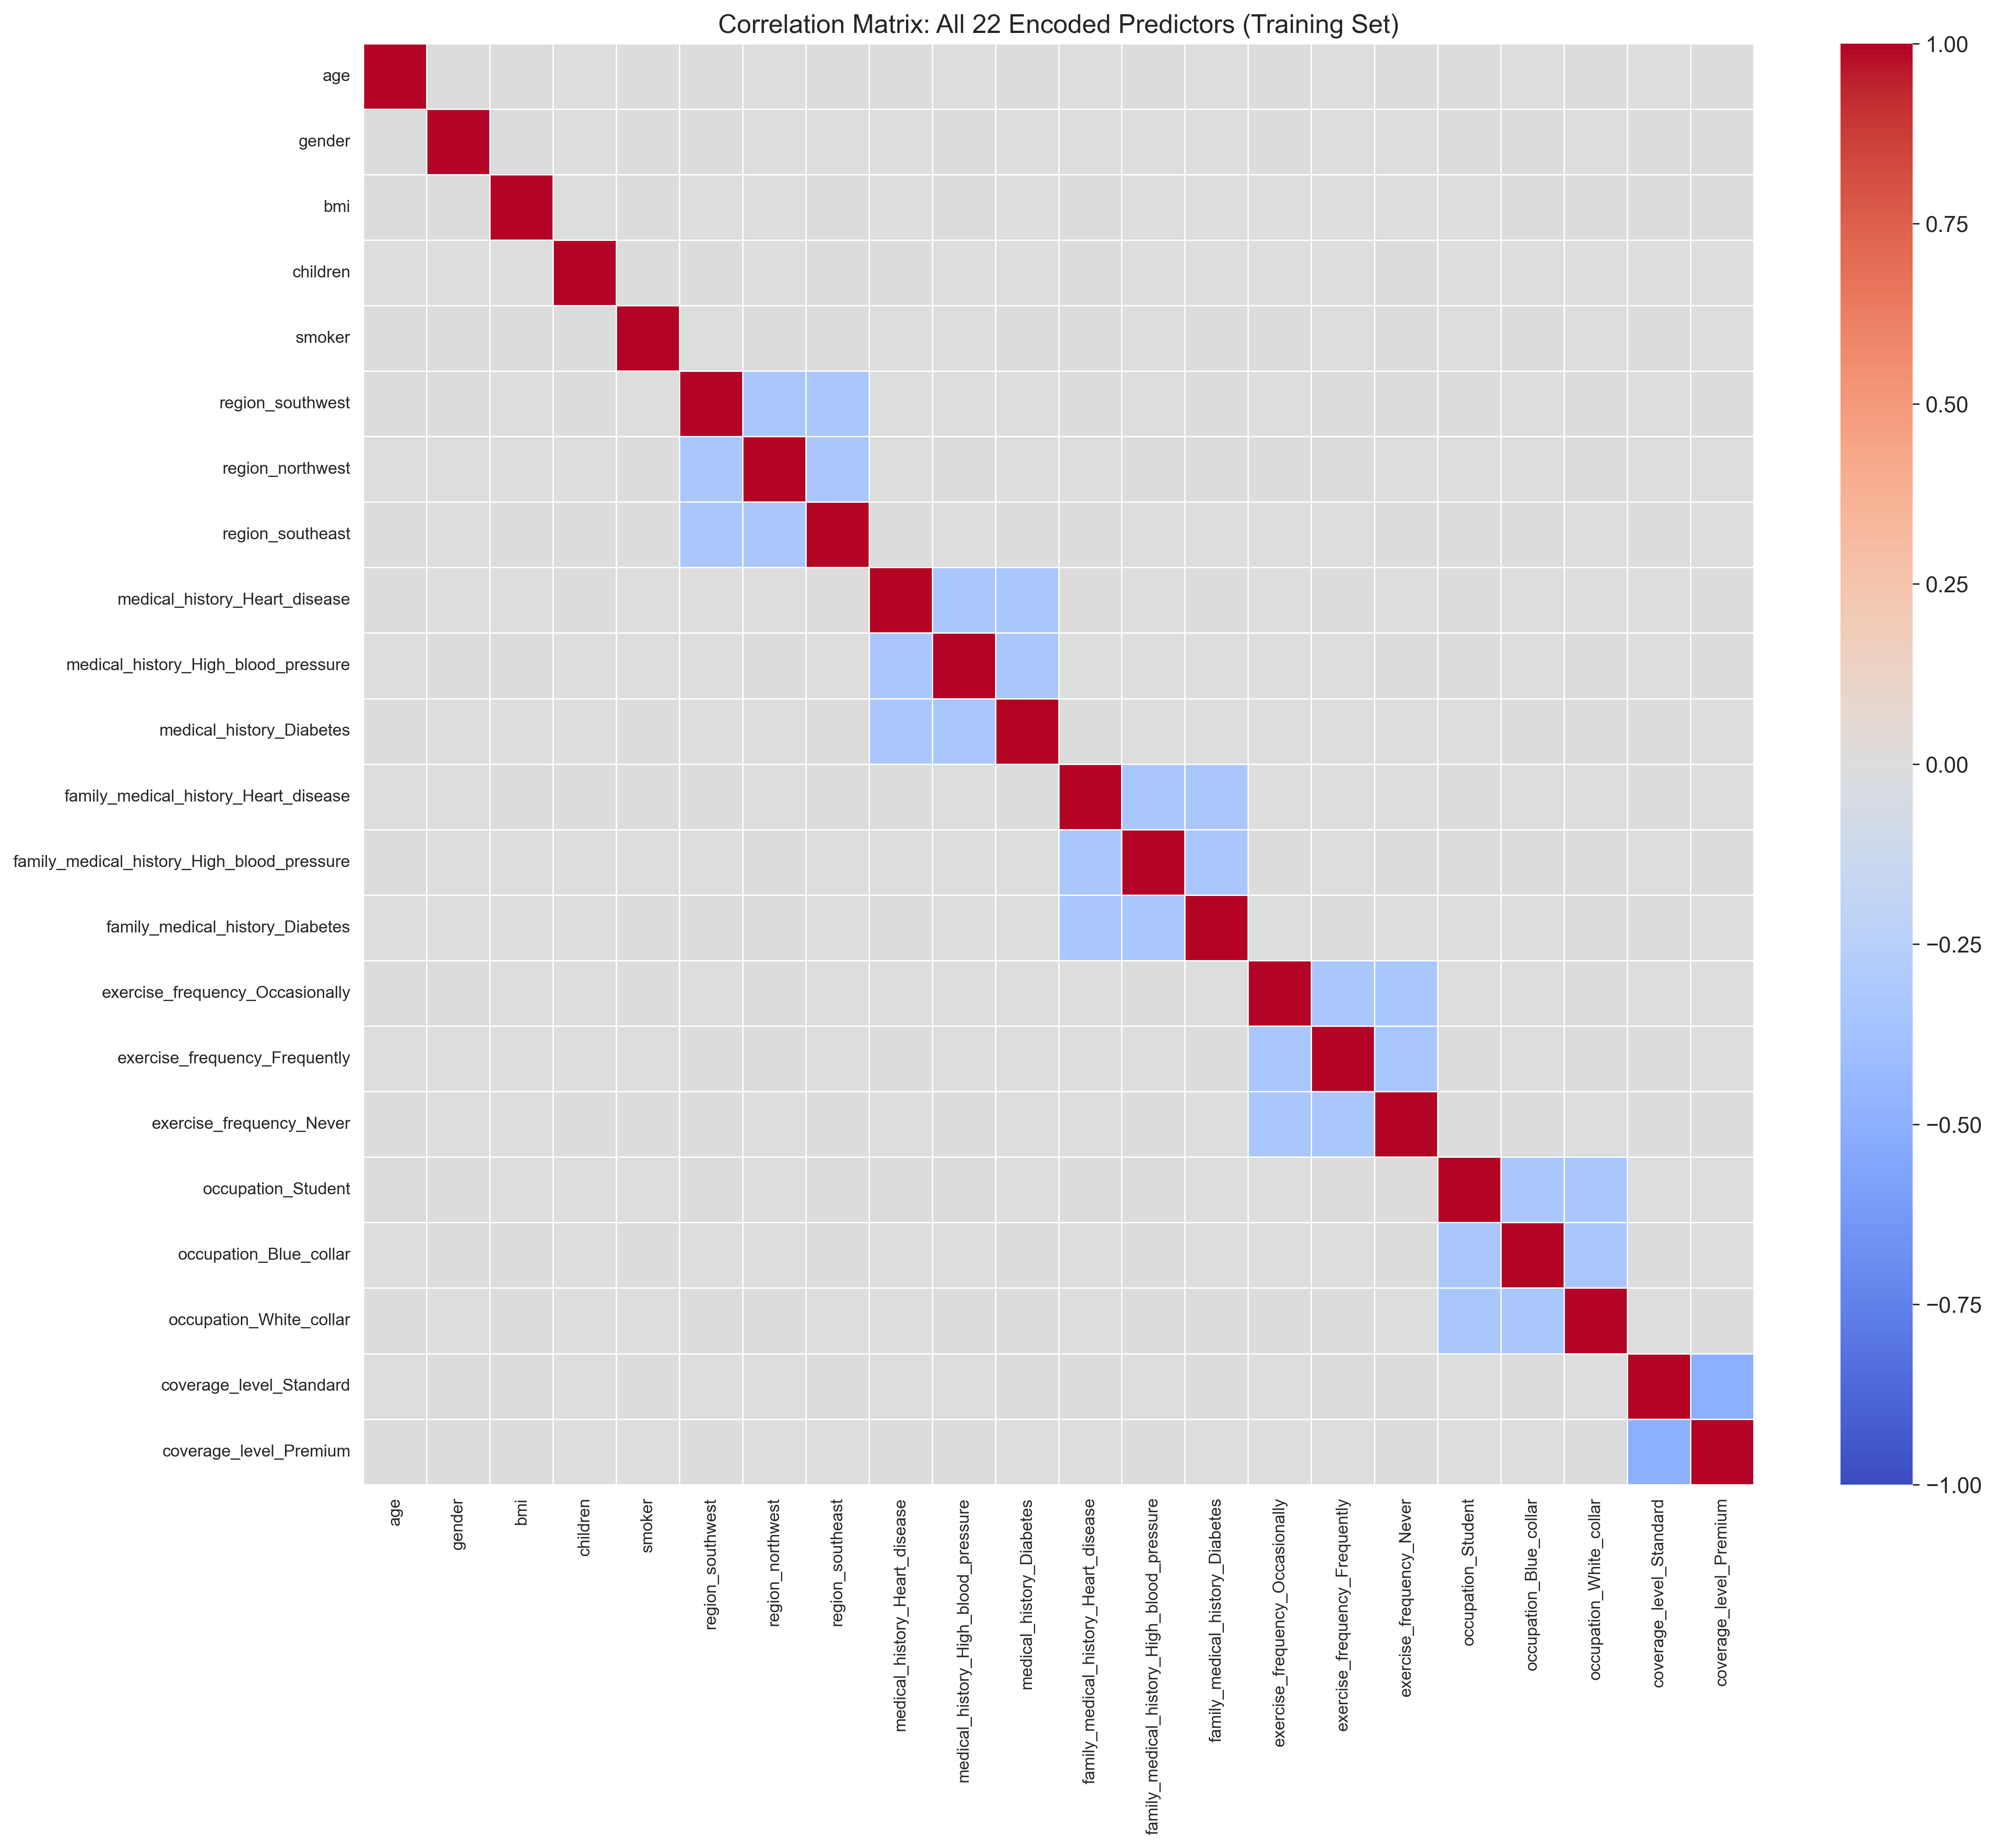
\includegraphics[width=\textwidth]{Thesis/Chapter 3/Figures/fig_full_encoded_correlation_heatmap.png}
    \caption{Full $22 \times 22$ Pearson correlation matrix of encoded predictors.}
    \label{fig:full_encoded_correlation_heatmap_ch3}
\end{subfigure}
\caption{Encoded predictor correlation analysis on the training partition.}
\label{fig:encoded_correlation_analysis_ch3}
\end{figure}

\noindent
Figure~\ref{fig:encoded_correlations_ch3} ranks all 22 encoded predictors
by their Pearson correlation with \texttt{charges}. The four strongest
positive associations are \texttt{smoker} ($r = 0.567$),\allowbreak{}
\texttt{coverage\_level\_\allowbreak{}Premium} ($r \approx 0.43$),\allowbreak{}
\texttt{medical\_history\_\allowbreak{}Heart\_disease} ($r \approx 0.39$) and
\texttt{family\_medical\_\allowbreak{}history\_\allowbreak{}Heart\_disease} ($r \approx 0.39$).
A second tier of moderate positive associations includes
\texttt{exercise\_frequency\_\allowbreak{}Frequently} ($r \approx 0.15$),\allowbreak{}
\texttt{occupation\_\allowbreak{}White\_collar} ($r \approx 0.12$),\allowbreak{}
\texttt{bmi}
($r \approx 0.10$), \texttt{children} ($r \approx 0.08$) and \texttt{age}
($r \approx 0.06$). On the negative side, the largest associations are
\texttt{medical\_history\_\allowbreak{}High\_blood\_\allowbreak{}pressure} ($r \approx -0.11$),\allowbreak{}
\texttt{family\_medical\_\allowbreak{}history\_\allowbreak{}High\_blood\_\allowbreak{}pressure}
($r \approx -0.10$),\allowbreak{}
\texttt{exercise\_frequency\_\allowbreak{}Never}
($r \approx -0.09$) and \texttt{gender} ($r \approx -0.08$). These
negative values reflect the reference-category encoding: for example,
a negative correlation for
\texttt{medical\_history\_\allowbreak{}High\_blood\_\allowbreak{}pressure} indicates lower charges
relative to the omitted reference category rather than a protective effect.
Figure~\ref{fig:full_encoded_correlation_heatmap_ch3} shows the full
inter-predictor correlation structure. The dominant feature is the block
of negative correlations within each dummy group: dummy indicators derived
from the same raw categorical variable are mechanically negatively
correlated because only one indicator can be active at a time. Outside
these within-group blocks, the off-diagonal correlations are uniformly
near zero (grey shading), confirming the absence of problematic
multicollinearity among predictors from different raw variables.

% ----------------------------
% 3.3.4 PARTITION CONSISTENCY
% ----------------------------

\subsubsection{Partition consistency}
Kernel density estimates of \texttt{charges} and of each numerical
predictor were overlaid for the training, validation, and test partitions;
the distributions are virtually indistinguishable.  Proportions of each
dummy variable were likewise compared, and no systematic shifts are
present.  The partitioning procedure therefore preserves the
distributional characteristics of the data.

% -------------------------------------------------
% 3.3.5 DECISIONS FROM THE EXPLORATORY DIAGNOSTICS
% -------------------------------------------------

\subsubsection{Decisions from the exploratory diagnostics}
Four implementation decisions follow directly from the EDA:

\begin{enumerate}
    \item Bounded numerical predictors are simulated under support
          restrictions that maintain their observed ranges.
    \item Categorical variables are simulated at the raw-category level
          and only afterwards encoded.
    \item The weak linear correlations among the numerical predictors,
          together with their uniform-like marginal shapes, motivate the
          product-marginal independence assumption adopted in the \gls{mc}
          design (Section~\ref{sec:mc_simulation_design}).
    \item The response is standardised during training and de-normalised
          for evaluation; no further transformation is needed.
\end{enumerate}

% ----------------------------------------
% 3.4 Network Specification and Training
% ----------------------------------------
\subsection{Network Specification and Training}
\label{sec:dnn_specification_training}

The predictive component is a \gls{dnn} for supervised
regression, following the formulation of equations~\eqref{eq:regression}
and~\eqref{eq:fitted_model}.  The network maps the model-ready input vector
$\mathbf{z}_i \in \mathbb{R}^{22}$ to a scalar prediction of the
standardised response,
\begin{equation}
    \widehat{\widetilde{y}}_i = f_{\widehat{\theta}}(\mathbf{z}_i),
    \label{eq:dnn_prediction_standardised_ch3}
\end{equation}
\equationlistentry{\Gls{dnn} prediction on standardised scale}
which is subsequently de-normalised to the original monetary scale via
equation~\eqref{eq:response_denormalisation_ch3}.

\subsubsection{Architecture}

The network adopts the contracting funnel topology

\begin{figure}[htbp]                                                                                                                                                                                               
  \centering                                                                                                                                                                                                       
  \begin{tikzpicture}[                                                                                                                                                                                               
      neuron/.style={circle, draw=black, fill=white, minimum size=10pt,                                                                                                                                            
                     inner sep=0pt, line width=0.4pt},                                                                                                                                                               
      dots/.style={minimum size=10pt, inner sep=0pt},                                                                                                                                                              
      layer label/.style={font=\footnotesize\bfseries, align=center},
      width label/.style={font=\scriptsize, text=black!70},
      connection/.style={-, draw=black!20, line width=0.2pt},
  ]

  % ── Horizontal positions ──
  \def\xIn{0}
  \def\xA{1.6}
  \def\xB{3.2}
  \def\xC{4.8}
  \def\xD{6.4}
  \def\xE{8.0}
  \def\xOut{9.6}

  % ── Vertical half-spans (centred at y = 0) ──
  \def\sIn{0.7}    % 22
  \def\sA{3.2}     % 256
  \def\sB{2.4}     % 128
  \def\sC{1.7}     % 64
  \def\sD{1.1}     % 32
  \def\sE{0.65}    % 16

  % === INPUT (22) ===
  \node[neuron] (i1) at (\xIn,  \sIn) {};
  \node[neuron] (i2) at (\xIn,  \sIn*0.33) {};
  \node[dots]        at (\xIn, -\sIn*0.2) {$\vdots$};
  \node[neuron] (i3) at (\xIn, -\sIn*0.55) {};
  \node[neuron] (i4) at (\xIn, -\sIn) {};
  \node[layer label, above=4pt of i1] {Input};
  \node[width label, below=4pt of i4] {22};

  % === HIDDEN 1 (256) ===
  \node[neuron] (a1) at (\xA,  \sA) {};
  \node[neuron] (a2) at (\xA,  \sA*0.65) {};
  \node[dots]        at (\xA,  \sA*0.35) {$\vdots$};
  \node[dots]        at (\xA,  0) {$\vdots$};
  \node[dots]        at (\xA, -\sA*0.35) {$\vdots$};
  \node[neuron] (a3) at (\xA, -\sA*0.65) {};
  \node[neuron] (a4) at (\xA, -\sA) {};
  \node[layer label, above=4pt of a1] {Hidden 1};
  \node[width label, below=4pt of a4] {256};

  % === HIDDEN 2 (128) ===
  \node[neuron] (b1) at (\xB,  \sB) {};
  \node[neuron] (b2) at (\xB,  \sB*0.55) {};
  \node[dots]        at (\xB,  0) {$\vdots$};
  \node[dots]        at (\xB, -\sB*0.3) {$\vdots$};
  \node[neuron] (b3) at (\xB, -\sB*0.65) {};
  \node[neuron] (b4) at (\xB, -\sB) {};
  \node[layer label, above=4pt of b1] {Hidden 2};
  \node[width label, below=4pt of b4] {128};

  % === HIDDEN 3 (64) ===
  \node[neuron] (c1) at (\xC,  \sC) {};
  \node[neuron] (c2) at (\xC,  \sC*0.4) {};
  \node[dots]        at (\xC, -\sC*0.15) {$\vdots$};
  \node[neuron] (c3) at (\xC, -\sC*0.55) {};
  \node[neuron] (c4) at (\xC, -\sC) {};
  \node[layer label, above=4pt of c1] {Hidden 3};
  \node[width label, below=4pt of c4] {64};

  % === HIDDEN 4 (32) ===
  \node[neuron] (d1) at (\xD,  \sD) {};
  \node[neuron] (d2) at (\xD,  \sD*0.33) {};
  \node[dots]        at (\xD, -\sD*0.2) {$\vdots$};
  \node[neuron] (d3) at (\xD, -\sD*0.55) {};
  \node[neuron] (d4) at (\xD, -\sD) {};
  \node[layer label, above=4pt of d1] {Hidden 4};
  \node[width label, below=4pt of d4] {32};

  % === HIDDEN 5 (16) ===
  \node[neuron] (e1) at (\xE,  \sE) {};
  \node[neuron] (e2) at (\xE,  \sE*0.33) {};
  \node[dots]        at (\xE, -\sE*0.2) {$\vdots$};
  \node[neuron] (e3) at (\xE, -\sE*0.55) {};
  \node[neuron] (e4) at (\xE, -\sE) {};
  \node[layer label, above=4pt of e1] {Hidden 5};
  \node[width label, below=4pt of e4] {16};

  % === OUTPUT (1) ===
  \node[neuron] (o1) at (\xOut, 0) {};
  \node[layer label, above=4pt of o1] {Output};
  \node[width label, below=4pt of o1] {1};

  % === CONNECTIONS ===
  \foreach \src in {i1,i2,i3,i4}{
      \foreach \dst in {a1,a2,a3,a4}{ \draw[connection] (\src) -- (\dst); }}
  \foreach \src in {a1,a2,a3,a4}{
      \foreach \dst in {b1,b2,b3,b4}{ \draw[connection] (\src) -- (\dst); }}
  \foreach \src in {b1,b2,b3,b4}{
      \foreach \dst in {c1,c2,c3,c4}{ \draw[connection] (\src) -- (\dst); }}
  \foreach \src in {c1,c2,c3,c4}{
      \foreach \dst in {d1,d2,d3,d4}{ \draw[connection] (\src) -- (\dst); }}
  \foreach \src in {d1,d2,d3,d4}{
      \foreach \dst in {e1,e2,e3,e4}{ \draw[connection] (\src) -- (\dst); }}
  \foreach \src in {e1,e2,e3,e4}{
      \draw[connection] (\src) -- (o1); }

  \end{tikzpicture}
  \caption{Funnel architecture of the \gls{dnn}.}
  \label{fig:dnn_architecture_ch3}
  \end{figure}

with the layer-wise recursion given by
equation~\eqref{eq:pre_activation}.  All hidden layers use the
\gls{celu} activation function
(equation~\eqref{eq:celu}).  \gls{celu} was selected from among the
candidate activations reviewed in
Section~\ref{sec:activation_functions} because it combines the
computational efficiency of a rectifier with continuous
differentiability across its entire domain, avoiding the dead-unit
problem associated with \gls{relu} while maintaining a linear positive
branch that preserves gradient flow in deep architectures.  The output
layer uses an identity mapping, as required for continuous regression.  The full five-hidden-layer depth,
including the final 16-unit layer, is retained; its adequacy is assessed
through the validation diagnostics of
Section~\ref{sec:model_validation_diagnostics}.

The network is constructed without bias vectors.  This is a genuine
restriction rather than a costless simplification: because the \gls{celu}
activation satisfies $\sigma(0)=0$, a bias-free network necessarily maps
the origin to zero, so the fitted function is pinned to zero at the
standardised data centroid and cannot represent arbitrary additive shifts
(the corresponding universal-approximation caveat is discussed in
Chapter~\ref{sec:literature_review}).  After standardisation, however, the
data centroid maps near the origin, where the response surface lies well
within the support of the data, and the adequacy of the bias-free
restriction is assessed empirically through the predictive diagnostics of
Section~\ref{sec:model_validation_diagnostics} rather than guaranteed
theoretically.  The total number of trainable parameters is
\begin{align}
    N_{\mathrm{par}}
    &= (22)(256) + (256)(128) + (128)(64) + (64)(32) + (32)(16) + (16)(1) \notag \\
    &= 49\,168.
    \label{eq:dnn_parameter_count_ch3}
\end{align}
\equationlistentry{\Gls{dnn} total trainable parameter count}

\subsubsection{Forward and Backward Propagation}
\label{sec:propagation_mechanics}

The operation of the contracting funnel specified in figure
\ref{fig:dnn_architecture_ch3} can be described compactly by the
forward- and backward-pass equations that underpin all gradient-based
training.  For a single input vector $\mathbf{x}$ (with
$\mathbf{a}^{(0)} = \mathbf{x}$), the forward computation of layer $l$ is
\begin{align}
    \mathbf{z}^{(l)} &= \bigl(W^{(l)}\bigr)^{\!\top} \mathbf{a}^{(l-1)}
                      + \mathbf{b}^{(l)},
                      \qquad
                      W^{(l)} \in \mathbb{R}^{d_{l-1}\times d_{l}},\;
                      \mathbf{b}^{(l)} \in \mathbb{R}^{d_{l}},
    \label{eq:forward_affine} \\
    \mathbf{a}^{(l)} &= \sigma_l\!\bigl(\mathbf{z}^{(l)}\bigr),
    \label{eq:forward_activation}
\end{align}
where $d_{l-1}$ and $d_{l}$ are the widths of the adjacent layers.
Because the input and response are standardised and the architecture omits
bias vectors (Section~\ref{sec:dnn_specification_training}), the bias term
is not used; the forward pass simplifies to
equation~\eqref{eq:bias_free_recursion}.

The network is trained by minimising the \gls{mse} loss
$\mathcal{L} = \frac{1}{2}(y - \hat{y})^{2}$.  Defining the gradient of the
loss with respect to the output pre-activation as
\begin{equation}
    \delta^{(L)} \equiv \frac{\partial \mathcal{L}}{\partial \mathbf{z}^{(L)}}
    = \hat{y} - y,
    \label{eq:output_delta}
\end{equation}
this error signal is propagated backward through the hidden layers.  For
layer $l = L-1, L-2, \dots, 1$, the recursion is
\begin{equation}
    \delta^{(l)}
    = \frac{\partial \mathcal{L}}{\partial \mathbf{z}^{(l)}}
    = \bigl(W^{(l+1)}\bigr)^{\!\top} \delta^{(l+1)}
      \odot \sigma_{l}'\!\bigl(\mathbf{z}^{(l)}\bigr),
    \label{eq:backprop_delta}
\end{equation}
where $\odot$ denotes element-wise multiplication and $\sigma_{l}'$ is the
derivative of the activation function.  For the \gls{celu} activation
employed in every hidden layer (equation~\eqref{eq:celu}), the derivative is
smooth and non-zero for all inputs, ensuring stable gradient flow.

The gradient of the loss with respect to the weight matrix of layer $l$ is
\begin{equation}
    \frac{\partial \mathcal{L}}{\partial W^{(l)}}
    = \mathbf{a}^{(l-1)} \bigl(\delta^{(l)}\bigr)^{\!\top}.
    \label{eq:weight_gradient}
\end{equation}
Because bias vectors are omitted, no bias-update term appears.  The weight
matrices are then updated by the \gls{nadam} optimiser
(Section~\ref{sec:training_configuration}), which combines Nesterov-accelerated momentum with adaptive learning rates.

These equations are standard in the deep learning literature
\citep{goodfellow2016deep} and are reproduced here for completeness; they
make the training procedure, including the bias-free simplification,
explicit.  In practice, all gradients are computed automatically by
the deep learning framework (PyTorch) through reverse-mode automatic
differentiation, so the closed-form expressions are never coded directly.
Their inclusion ensures that the reader can relate the chosen architecture,
loss function, and activation to the mechanics of gradient-based
optimisation.


\subsubsection{Training configuration}
\label{sec:training_configuration}

The network is trained by minimising the \gls{mse} on the
standardised response scale (equation~\eqref{eq:mse_loss}).  Weights are
updated with the \gls{nadam} optimiser \citep{dozat2016incorporating}, described
in Section~\ref{sec:loss_optimisation}.  Validation performance is
evaluated every $v = 5$ epochs.  For a fixed validation set, minimising
the validation \gls{mse} is equivalent to maximising the validation \gls{r2}; the
dot-product \gls{r2} is therefore used as the operational model-selection
criterion.  The selected epoch is
\begin{equation}
    e^{*} = \arg\max_{e \in \mathcal{E}_{\mathrm{val}}} R^2_{\mathrm{val}}(e),
    \qquad
    \mathcal{E}_{\mathrm{val}} = \{v, 2v, 3v, \dots\} \cap \{1, \dots, E_{\max}\}.
    \label{eq:validation_r2_epoch_selection_ch3}
\end{equation}
\equationlistentry{Validation $R^2$ epoch selection criterion}
Training stops early if the validation \gls{r2} does not improve for $P = 10$
consecutive validation checks \citep{prechelt2012early}; the retained
model is the checkpoint with the highest validation \gls{r2} observed.  The test set is reserved
exclusively for final out-of-sample evaluation.

On the original monetary scale, the standard
$R^2 = 1 - \mathrm{SS}_{\mathrm{res}} / \mathrm{SS}_{\mathrm{tot}}$
(equation~\eqref{eq:r_squared}) is reported alongside the \gls{mae} and
\gls{rmse}.

Table~\ref{tab:dnn_architecture_training_ch3} summarises the complete
architecture and training configuration.

\begin{table}[H]
\centering
\small
\renewcommand{\arraystretch}{1.15}
\begin{tabular}{p{0.34\textwidth}p{0.56\textwidth}}
\toprule
\textbf{Component} & \textbf{Specification} \\
\midrule
Input dimension & $p = 22$ encoded predictor variables \\
Hidden layer widths & $256, 128, 64, 32, 16$ \\
Output dimension & One scalar regression output \\
Architecture type & Fully connected \gls{dnn} \\
Network shape & Contracting representation from 256 to 16 hidden units \\
Bias vectors & Omitted \\
Hidden activation & \gls{celu} (equation~\eqref{eq:celu}) \\
Output activation & Identity mapping \\
Training response & Standardised \texttt{charges} \\
Prediction scale & De-normalised to the original monetary scale \\
Training objective & \Gls{mse} on the standardised response scale \\
Secondary evaluation metrics & \gls{mae}, \gls{rmse} and \gls{r2} on the original response scale \\
Optimiser & \gls{nadam} \citep{dozat2016incorporating} \\
Momentum parameters & $(\beta_1,\beta_2)$ selected by validation comparison from $\{(0.90,0.999),\ (0.95,0.999),\ (0.99,0.999)\}$ \\
Learning rate & Selected by validation comparison from $\{0.01, 0.001, 0.0005, 0.0001\}$ \\
Batch size & Selected by validation comparison from $\{64, 128, 256, 512\}$ \\
Maximum epochs & $E_{\max} = 200$ \\
Validation frequency & Every $v = 5$ epochs \\
Model-selection criterion & Dot-product validation \gls{r2} \\
Early stopping & Patience $P = 10$ validation checks without \gls{r2} improvement \\
Explicit regularisation & Not used \\
Dropout & Not used \\
Random seed & $s = 42$, fixed for reproducibility \\
Trainable parameters & $49\,168$ weights \\
\bottomrule
\end{tabular}
\caption{\Gls{dnn} architecture and training configuration.}
\label{tab:dnn_architecture_training_ch3}
\end{table}

\subsubsection{Hyperparameter comparison}

The main training hyperparameters that materially affect the fitted
prediction surface are compared sequentially:

\begin{enumerate}
    \item \textbf{Hidden activation:}  \gls{celu}, \gls{gelu} and Tanh are evaluated
          with learning rate $0.001$, batch size $256$, and \gls{adam} held fixed.
    \item \textbf{Learning rate:}  Values $\{0.01, 0.001, 0.0005, 0.0001\}$
          are tested with the best activation carried forward.
    \item \textbf{Batch size:}  Sizes $\{64, 128, 256, 512\}$ are tested
          with the best activation and learning rate.
    \item \textbf{Optimiser:}  \gls{adam} and \gls{nadam} are compared with all previous
          best choices carried forward.
    \item \textbf{Momentum parameters:} $(\beta_1,\beta_2)$.  Since \gls{nadam} is
          selected in the previous step, its Nesterov-accelerated momentum
          parameters are compared over
          $\{(0.90,0.999),\linebreak[1] (0.95,0.999),\linebreak[1] (0.99,0.999)\}$.  The first
          coefficient $\beta_1$ controls the decay of the gradient mean
          estimate; the second, $\beta_2$, controls the decay of the
          uncentred variance estimate \citep{dozat2016incorporating}.
\end{enumerate}

At each stage the best choice is carried forward and all other factors are
held constant.  Explicit $\mathcal{L}_1$, $\mathcal{L}_2$, and dropout
\citep{srivastava2014dropout} regularisation are not
included; the adequacy of this design is assessed through validation
curves, out-of-sample error metrics, and structural diagnostics\footnote{In this context, $\mathcal{L}_1$ and $\mathcal{L}_2$
regularisation refer to adding penalty terms to the training objective. If
\(\mathcal{L}_{0}(\theta)\) denotes the original training loss and
\(\theta=(\theta_1,\ldots,\theta_d)\) denotes the vector of trainable
parameters, then $\mathcal{L}_1$ regularisation uses
\[
    \mathcal{L}_{1}(\theta)
    =
    \mathcal{L}_{0}(\theta)
    +
    \lambda
    \sum_{j=1}^{d}
    |\theta_j|,
\]
whereas $\mathcal{L}_2$ regularisation uses
\[
    \mathcal{L}_{2}(\theta)
    =
    \mathcal{L}_{0}(\theta)
    +
    \lambda
    \sum_{j=1}^{d}
    \theta_j^2.
\]
Here, \(\lambda \geq 0\) controls the strength of the penalty. The $\mathcal{L}_1$
penalty encourages sparse parameter estimates, while the $\mathcal{L}_2$ penalty
shrinks parameters towards zero without necessarily setting them exactly equal
to zero.}.

The training procedure consists of: (1)~random weight initialisation
using Kaiming uniform initialisation \citep{he2015delving}, which
scales the initial weights according to the fan-in of each layer so
that activations neither vanish nor explode during the early forward
passes, a property that is particularly important in deeper
architectures such as the five-hidden-layer network used here;
(2)~mini-batch gradient descent with the \gls{nadam} optimiser;
(3)~validation evaluation every 5 epochs using the dot-product \gls{r2};
(4)~early stopping when the validation \gls{r2} has not improved for 10
consecutive checks; (5)~selection of the checkpoint with the highest
validation \gls{r2}; and (6)~final test-set evaluation on the original
monetary scale using \gls{r2}, \gls{rmse} and \gls{mae}.  The complete
pseudocode is presented in
Algorithm~\ref{tab:dnn_training_algorithm_annex}
(\ref{annexure:dnn_algorithm_detailed}).

\subsubsection{Benchmark GLM}
\label{sec:glm_benchmark_methods}

A classical actuarial benchmark is provided by a \gls{glm}
with a gamma distribution and logarithmic link function
\citep{dobson2008introduction, mccullagh1989generalized}.  For a policyholder with
model-ready input vector $\mathbf{z}_i \in \mathbb{R}^{22}$ (the same encoded
predictors used by the \gls{dnn}), the \gls{glm} assumes
\begin{equation}
    Y_i \sim \text{Gamma}(\mu_i, \phi),
    \qquad
    \log(\mu_i) = \beta_0 + \sum_{j=1}^{22} \beta_j z_{ij},
    \label{eq:glm_specification}
\end{equation}
\equationlistentry{\Gls{glm} specification with gamma distribution and log link}
where $\mu_i = \mathbb{E}[Y_i \mid \mathbf{z}_i]$ and $\phi$ is the
dispersion parameter.  The distributional and link-function rationale
for this specification was set out in
Section~\ref{sec:classical_actuarial}; under the log link the predicted
mean $\mu_i = \exp(\beta_0 + \sum_j \beta_j z_{ij})$ is always positive.

The model includes no interaction terms or non-linear transformations.  It
is fitted to the training partition by maximum likelihood estimation.  The
log-likelihood for the gamma \gls{glm} is
\begin{equation}
    \ell(\boldsymbol{\beta}, \phi)
    =
    \sum_{i=1}^{n}
    \left[
        \frac{1}{\phi}
        \left(
            -\frac{y_i}{\mu_i} - \log \mu_i
        \right)
        +
        \left(\frac{1}{\phi} - 1\right) \log y_i
        -
        \log \Gamma\!\left(\frac{1}{\phi}\right)
        -
        \frac{1}{\phi}\log \phi
    \right],
    \label{eq:glm_loglikelihood}
\end{equation}
\equationlistentry{Gamma \gls{glm} log-likelihood}
where $\mu_i = \exp(\mathbf{z}_i^{\top}\boldsymbol{\beta})$ and
$\boldsymbol{\beta} = (\beta_0, \beta_1, \ldots, \beta_{22})^{\top}$.
The parameter vector $\boldsymbol{\beta}$ is estimated by \gls{irls}, which solves the score equations
\begin{equation}
    \sum_{i=1}^{n}
    \frac{(y_i - \mu_i)}{\mathrm{Var}(Y_i)}
    \,
    \frac{\partial \mu_i}{\partial \eta_i}
    \,
    z_{ij}
    = 0,
    \qquad j = 0, 1, \ldots, 22,
    \label{eq:glm_score}
\end{equation}
\equationlistentry{\Gls{glm} score equations}
where $\eta_i = \log(\mu_i)$ is the linear predictor and
$\mathrm{Var}(Y_i) = \phi\,\mu_i^{2}$ under the gamma family.  Each \gls{irls}
iteration computes a weighted least squares regression of an adjusted
dependent variable on the design matrix, with weights inversely
proportional to the variance function evaluated at the current fitted
values \citep{dobson2008introduction}.

Algorithm~\ref{tab:glm_algorithm_annex} formalises the fitting procedure.

The \gls{glm} is fitted via \gls{irls},
which computes working weights and adjusted dependent variables at each
iteration until convergence.  The dispersion parameter
$\widehat{\phi}$ is estimated from the Pearson residuals, and
predictions are obtained on the original monetary scale by applying the
inverse link $\widehat{y}_i = \exp(\mathbf{z}_i^{\top}
\widehat{\boldsymbol{\beta}})$.  The complete \gls{irls} algorithm is
presented in Algorithm~\ref{tab:glm_algorithm_annex}
(\ref{annexure:glm_algorithm}).

No hyperparameter tuning is applied to the \gls{glm}; its role as a benchmark
was motivated in Section~\ref{sec:statistical_learning_supervised_regression}.

\subsubsection{Tree-Based Benchmarks}
\label{sec:tree_benchmarks_methods}

Two tree-based ensemble methods are included alongside the \gls{glm} to
provide a more comprehensive model-class comparison.  Both models use the
same 22 encoded features and the same approximately $52/24/24$ partition
(Section~\ref{sec:feature_encoding_input_standardisation}) as the
\gls{dnn} and \gls{glm}.

% ----- \Gls{rf} -----

\subsubsection{RF Benchmark}
A \gls{rf} regressor \citep{breiman2001random} is fitted with 500 trees,
maximum depth unrestricted, minimum samples per leaf of 5, and
\texttt{random\_state=42}.  \gls{rf} aggregates predictions across
decorrelated decision trees, reducing variance through bootstrap
aggregation (bagging) while maintaining low bias.

The \gls{rf} constructs an ensemble of $B$ regression trees, each grown on
a bootstrap sample of the training data.  At every candidate split the
algorithm considers only a random subset of $m$ out of $p$ predictors,
thereby decorrelating the individual trees and reducing the variance of the
averaged prediction.  For a regression tree $T_b$ grown on bootstrap
sample $\mathcal{D}_b^{*}$, the prediction for input $\mathbf{z}$ is
$\hat{y}_b(\mathbf{z}) = T_b(\mathbf{z})$.  The \gls{rf} prediction is
the average across all $B$ trees:
\begin{equation}
    \hat{f}_{\mathrm{RF}}(\mathbf{z})
    =
    \frac{1}{B}
    \sum_{b=1}^{B}
    T_b(\mathbf{z}).
    \label{eq:rf_prediction}
\end{equation}
\equationlistentry{\Gls{rf} ensemble prediction}

Each tree $T_b$ is grown by recursively partitioning the feature space.
At each internal node, the algorithm selects a random subset of
$m = \lfloor p/3 \rfloor$ predictors (the default for regression) and
chooses the split variable $j^{*}$ and split point $s^{*}$ that minimise
the weighted sum of squared residuals in the resulting child nodes:
\begin{equation}
    (j^{*}, s^{*})
    =
    \arg\min_{j \in \mathcal{S},\; s}
    \Biggl[
        \sum_{i:\, z_{ij} \le s} (y_i - \bar{y}_{L})^{2}
        +
        \sum_{i:\, z_{ij} > s} (y_i - \bar{y}_{R})^{2}
    \Biggr],
    \label{eq:rf_split_criterion}
\end{equation}
\equationlistentry{\Gls{rf} split criterion}
where $\mathcal{S} \subset \{1,\dots,p\}$ with $|\mathcal{S}| = m$ is the
randomly selected predictor subset, and $\bar{y}_{L}$ and $\bar{y}_{R}$
denote the sample means in the left and right child nodes respectively.
Trees are grown until each terminal node contains at most 5 observations.

The variance reduction mechanism of the \gls{rf} can be understood
through the decomposition of the variance of the ensemble average.  If
individual tree predictions have variance $\sigma^{2}$ and pairwise
correlation $\rho$, then
\begin{equation}
    \mathrm{Var}\bigl(\hat{f}_{\mathrm{RF}}\bigr)
    =
    \rho\,\sigma^{2}
    +
    \frac{1 - \rho}{B}\,\sigma^{2}.
    \label{eq:rf_variance_reduction}
\end{equation}
\equationlistentry{\Gls{rf} variance reduction}
As $B$ increases, the second term vanishes, and the ensemble variance is
governed by $\rho\,\sigma^{2}$.  By restricting splits to a random
predictor subset, the \gls{rf} reduces $\rho$ below the value obtained by
standard bagging (which uses all $p$ predictors at every split), yielding
a lower ensemble variance \citep{hastie2009elements}.

The complete training procedure is presented in
Algorithm~\ref{tab:rf_algorithm_annex}
(\ref{annexure:rf_algorithm}), and
Table~\ref{tab:rf_hyperparameters_ch3} summarises the \gls{rf}
configuration.

\begin{table}[H]
\centering
\small
\renewcommand{\arraystretch}{1.15}
\begin{tabular}{p{0.34\textwidth}p{0.56\textwidth}}
\toprule
\textbf{Component} & \textbf{Specification} \\
\midrule
Number of trees ($B$) & 500 \\
Candidate predictors per split ($m$) & $\lfloor p/3 \rfloor = 7$ \\
Maximum depth & Unrestricted \\
Minimum samples per leaf & 5 \\
Bootstrap sampling & With replacement, sample size $= n_{\mathrm{train}}$ \\
Split criterion & \Gls{mse} (equation~\eqref{eq:rf_split_criterion}) \\
Hyperparameter tuning & Not applied (default values) \\
Random seed & 42 \\
Implementation & \texttt{scikit-learn} \texttt{Random\allowbreak{}Forest\allowbreak{}Regressor} \\
\bottomrule
\end{tabular}
\caption{\Gls{rf} configuration.}
\label{tab:rf_hyperparameters_ch3}
\end{table}

% ----- XGBoost -----

\subsubsection{XGBoost Benchmark}
A gradient-boosted tree regressor is fitted using the \gls{xgboost}
implementation \citep{chen2016xgboost} with 1\,000 boosting rounds, a
learning rate of 0.05, maximum depth of 8, and early stopping on the
validation set with a patience of 50 rounds.  \gls{xgboost} constructs an
additive ensemble of shallow trees via gradient boosting, using
approximate histogram-based splitting for computational efficiency.

Gradient boosting builds an additive model in a stage-wise fashion.  The
ensemble prediction after $M$ boosting rounds is
\begin{equation}
    \hat{f}_{M}(\mathbf{z})
    =
    \sum_{m=0}^{M}
    \eta \, h_m(\mathbf{z}),
    \label{eq:xgb_additive_model}
\end{equation}
\equationlistentry{\Gls{xgboost} additive ensemble model}
where $h_0(\mathbf{z}) = \bar{y}$ is the initial constant prediction
(the training-set mean), $h_m$ is the regression tree fitted at round $m$,
and $\eta \in (0,1]$ is the learning rate (shrinkage parameter) that
scales each tree's contribution.

At each boosting round $m$, \gls{xgboost} fits a new tree $h_m$ to
minimise a regularised objective.  For the squared-error loss used in
regression, the objective at round $m$ is
\begin{equation}
    \mathcal{O}^{(m)}
    =
    \sum_{i=1}^{n}
    \ell\!\bigl(y_i,\, \hat{f}_{m-1}(\mathbf{z}_i) + h_m(\mathbf{z}_i)\bigr)
    +
    \Omega(h_m),
    \label{eq:xgb_objective}
\end{equation}
\equationlistentry{\Gls{xgboost} regularised objective}
where $\ell(y, \hat{y}) = \tfrac{1}{2}(y - \hat{y})^{2}$ is the
squared-error loss and $\Omega(h_m)$ is a regularisation penalty on the
complexity of tree $h_m$.  The regularisation term is defined as
\begin{equation}
    \Omega(h)
    =
    \gamma \, J
    +
    \tfrac{1}{2}\,\lambda
    \sum_{j=1}^{J}
    w_j^{2},
    \label{eq:xgb_regularisation}
\end{equation}
\equationlistentry{\Gls{xgboost} tree complexity penalty}
where $J$ is the number of terminal nodes (leaves), $w_j$ is the
predicted value in leaf $j$, $\gamma \ge 0$ penalises additional leaves,
and $\lambda \ge 0$ applies $\mathcal{L}_2$ shrinkage to the leaf weights.

The key computational innovation of \gls{xgboost} is the use of a
second-order Taylor expansion of the loss around the current prediction
$\hat{f}_{m-1}(\mathbf{z}_i)$.  Define the first- and second-order
gradient statistics for observation $i$:
\begin{equation}
    g_i
    =
    \frac{\partial\, \ell(y_i,\, \hat{y})}{\partial\, \hat{y}}
    \bigg|_{\hat{y} = \hat{f}_{m-1}(\mathbf{z}_i)},
    \qquad
    h_i
    =
    \frac{\partial^{2}\, \ell(y_i,\, \hat{y})}{\partial\, \hat{y}^{2}}
    \bigg|_{\hat{y} = \hat{f}_{m-1}(\mathbf{z}_i)}.
    \label{eq:xgb_gradient_hessian}
\end{equation}
\equationlistentry{\Gls{xgboost} gradient and Hessian statistics}
For the squared-error loss, $g_i = \hat{f}_{m-1}(\mathbf{z}_i) - y_i$
(the negative residual) and $h_i = 1$.  With these gradient statistics,
the approximate objective simplifies to
\begin{equation}
    \tilde{\mathcal{O}}^{(m)}
    =
    \sum_{j=1}^{J}
    \Biggl[
        G_j \, w_j
        +
        \frac{1}{2}(H_j + \lambda)\, w_j^{2}
    \Biggr]
    +
    \gamma \, J,
    \label{eq:xgb_approx_objective}
\end{equation}
\equationlistentry{\Gls{xgboost} second-order approximate objective}
where $G_j = \sum_{i \in I_j} g_i$ and $H_j = \sum_{i \in I_j} h_i$ are
the sums of gradient and Hessian statistics over the observations
$I_j$ assigned to leaf $j$.  The optimal leaf weight and the
corresponding optimal objective value are
\begin{equation}
    w_j^{*}
    =
    -\frac{G_j}{H_j + \lambda},
    \qquad
    \tilde{\mathcal{O}}^{*}
    =
    -\frac{1}{2}
    \sum_{j=1}^{J}
    \frac{G_j^{2}}{H_j + \lambda}
    +
    \gamma \, J.
    \label{eq:xgb_optimal_leaf}
\end{equation}
\equationlistentry{\Gls{xgboost} optimal leaf weight and objective}

To evaluate a candidate split that partitions observations in a node into
left ($I_L$) and right ($I_R$) child nodes, \gls{xgboost} computes the
gain:
\begin{equation}
    \mathrm{Gain}
    =
    \frac{1}{2}
    \left[
        \frac{G_L^{2}}{H_L + \lambda}
        +
        \frac{G_R^{2}}{H_R + \lambda}
        -
        \frac{(G_L + G_R)^{2}}{H_L + H_R + \lambda}
    \right]
    -
    \gamma,
    \label{eq:xgb_split_gain}
\end{equation}
\equationlistentry{\Gls{xgboost} split gain criterion}
where $G_L = \sum_{i \in I_L} g_i$, $G_R = \sum_{i \in I_R} g_i$,
$H_L = \sum_{i \in I_L} h_i$, and $H_R = \sum_{i \in I_R} h_i$.  A
split is made only if $\mathrm{Gain} > 0$; the regularisation parameter
$\gamma$ acts as a minimum-gain threshold that prunes unprofitable splits
\citep{chen2016xgboost}.

The complete training procedure is presented in
Algorithm~\ref{tab:xgb_algorithm_annex}
(\ref{annexure:xgb_algorithm}), and
Table~\ref{tab:xgb_hyperparameters_ch3} summarises the \gls{xgboost}
configuration.

\begin{table}[H]
\centering
\small
\renewcommand{\arraystretch}{1.15}
\begin{tabular}{p{0.34\textwidth}p{0.56\textwidth}}
\toprule
\textbf{Component} & \textbf{Specification} \\
\midrule
Maximum boosting rounds ($M$) & 1\,000 \\
Learning rate ($\eta$) & 0.05 \\
Maximum tree depth ($d_{\max}$) & 8 \\
Booster & \texttt{gbtree} (tree-based) \\
Objective & \texttt{reg:squarederror} \\
Split evaluation & Approximate histogram-based \\
$\mathcal{L}_2$ regularisation ($\lambda$) & Default (1.0) \\
Minimum split gain ($\gamma$) & Default (0.0) \\
Early stopping patience & 50 rounds on validation loss \\
Hyperparameter tuning & Not applied (default values) \\
Random seed & 42 \\
Implementation & \texttt{xgboost} \texttt{XGBRegressor} \\
\bottomrule
\end{tabular}
\caption{\Gls{xgboost} configuration.}
\label{tab:xgb_hyperparameters_ch3}
\end{table}

In the primary comparison, hyperparameters for both tree-based models are
set to commonly recommended defaults rather than tuned via
cross-validation, paralleling the no-tuning treatment of the \gls{glm};
this isolates model-class differences from tuning effort.  As a
complementary analysis, both tree-based models are subsequently re-fitted
with tuned hyperparameters selected by randomised search with five-fold
cross-validation on the training partition, quantifying how much of any
remaining performance gap is attributable to tuning rather than to the
model class itself (results in Section~\ref{sec:tuned_benchmarks}).  All
models are evaluated using $R^2$, \gls{rmse} and \gls{mae} on the
original monetary scale across all three partitions.

% =============================================================
\subsection{Predictive and Structural Diagnostics}
\label{sec:model_validation_diagnostics}
\label{sec:model_evaluation_metrics}
\label{sec:fitted_model_diagnostic_plots}

The predictive and structural diagnostics described below serve a single
purpose: to verify that the fitted \gls{dnn} is sufficiently stable and
well-behaved to act as the prediction surface in the subsequent \gls{mc}
and Shapley-value analyses.

All predictive performance metrics are computed on the original monetary
scale after de-normalising the fitted predictions.  The metrics are the
\gls{mae}, \gls{rmse} and $R^2$ defined in
equations~\eqref{eq:mae},~\eqref{eq:rmse} and~\eqref{eq:r_squared}.  For
observation $i$ the fitted prediction is denoted $\widehat{y}_i$ and
the residual is
\begin{equation}
    r_i = y_i - \widehat{y}_i .
    \label{eq:residual_definition_ch3}
\end{equation}
\equationlistentry{Residual definition}
Residuals are computed separately for the training, validation and test
partitions.

\subsubsection{Predictive error assessment}

Predictive error is assessed by comparing observed charges with fitted
predictions on the original response scale.  The training partition is used
to evaluate in-sample fit, the validation partition to guide model-selection
decisions, and the test partition to provide a final out-of-sample
evaluation.  The three scalar metrics are interpreted jointly: a suitable
model should exhibit consistent performance across the validation and test
partitions, without a large deterioration relative to the training
partition.

\begin{figure}[H]
\centering
\begin{subfigure}[b]{\textwidth}
    \centering
    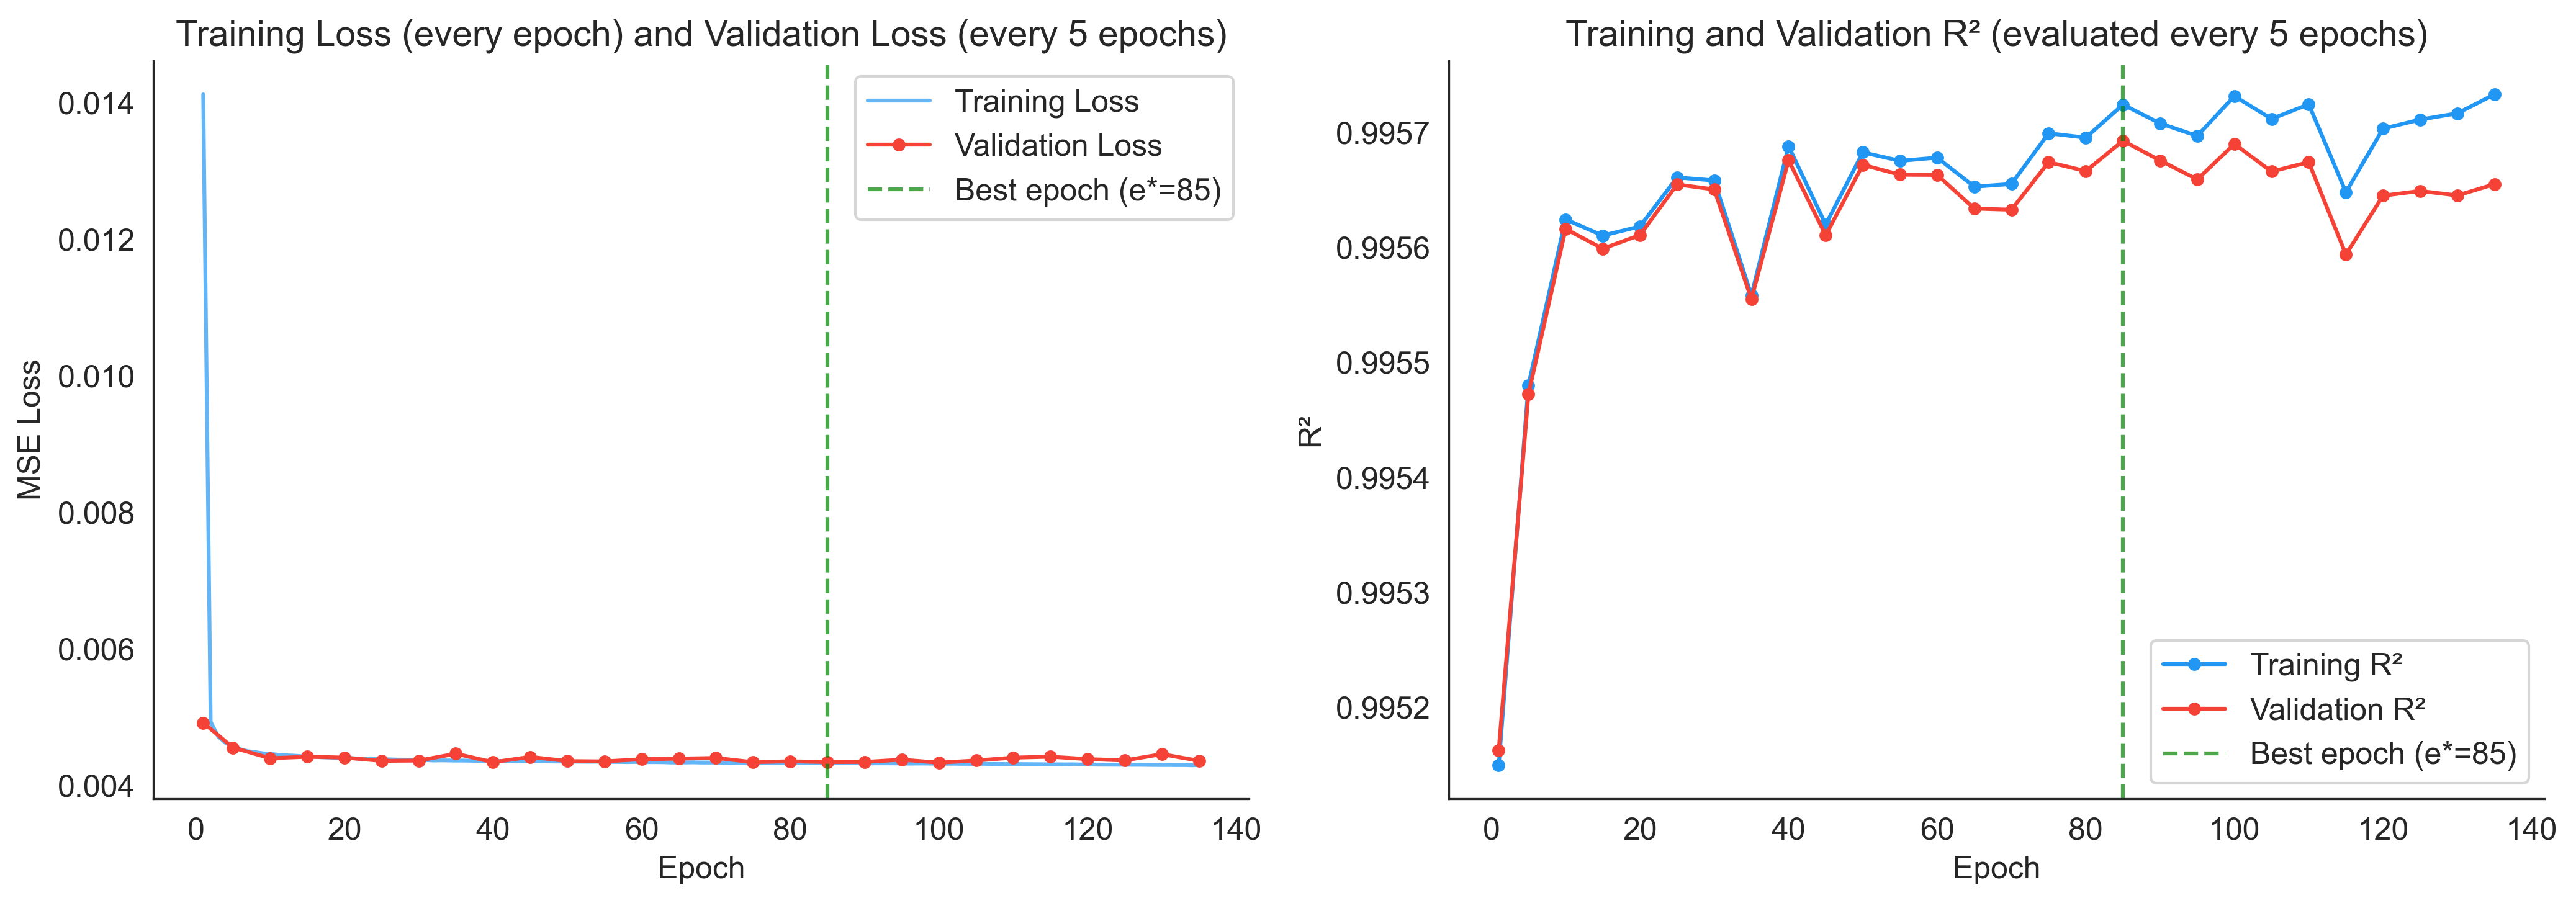
\includegraphics[width=0.90\textwidth]{Thesis/Chapter 3/Figures/fig_training_validation_curves.png}
    \caption{Training and validation loss with $R^2$ over epochs.}
    \label{fig:learning_curves_ch3}
\end{subfigure}

\vspace{0.4cm}

\begin{subfigure}[b]{\textwidth}
    \centering
    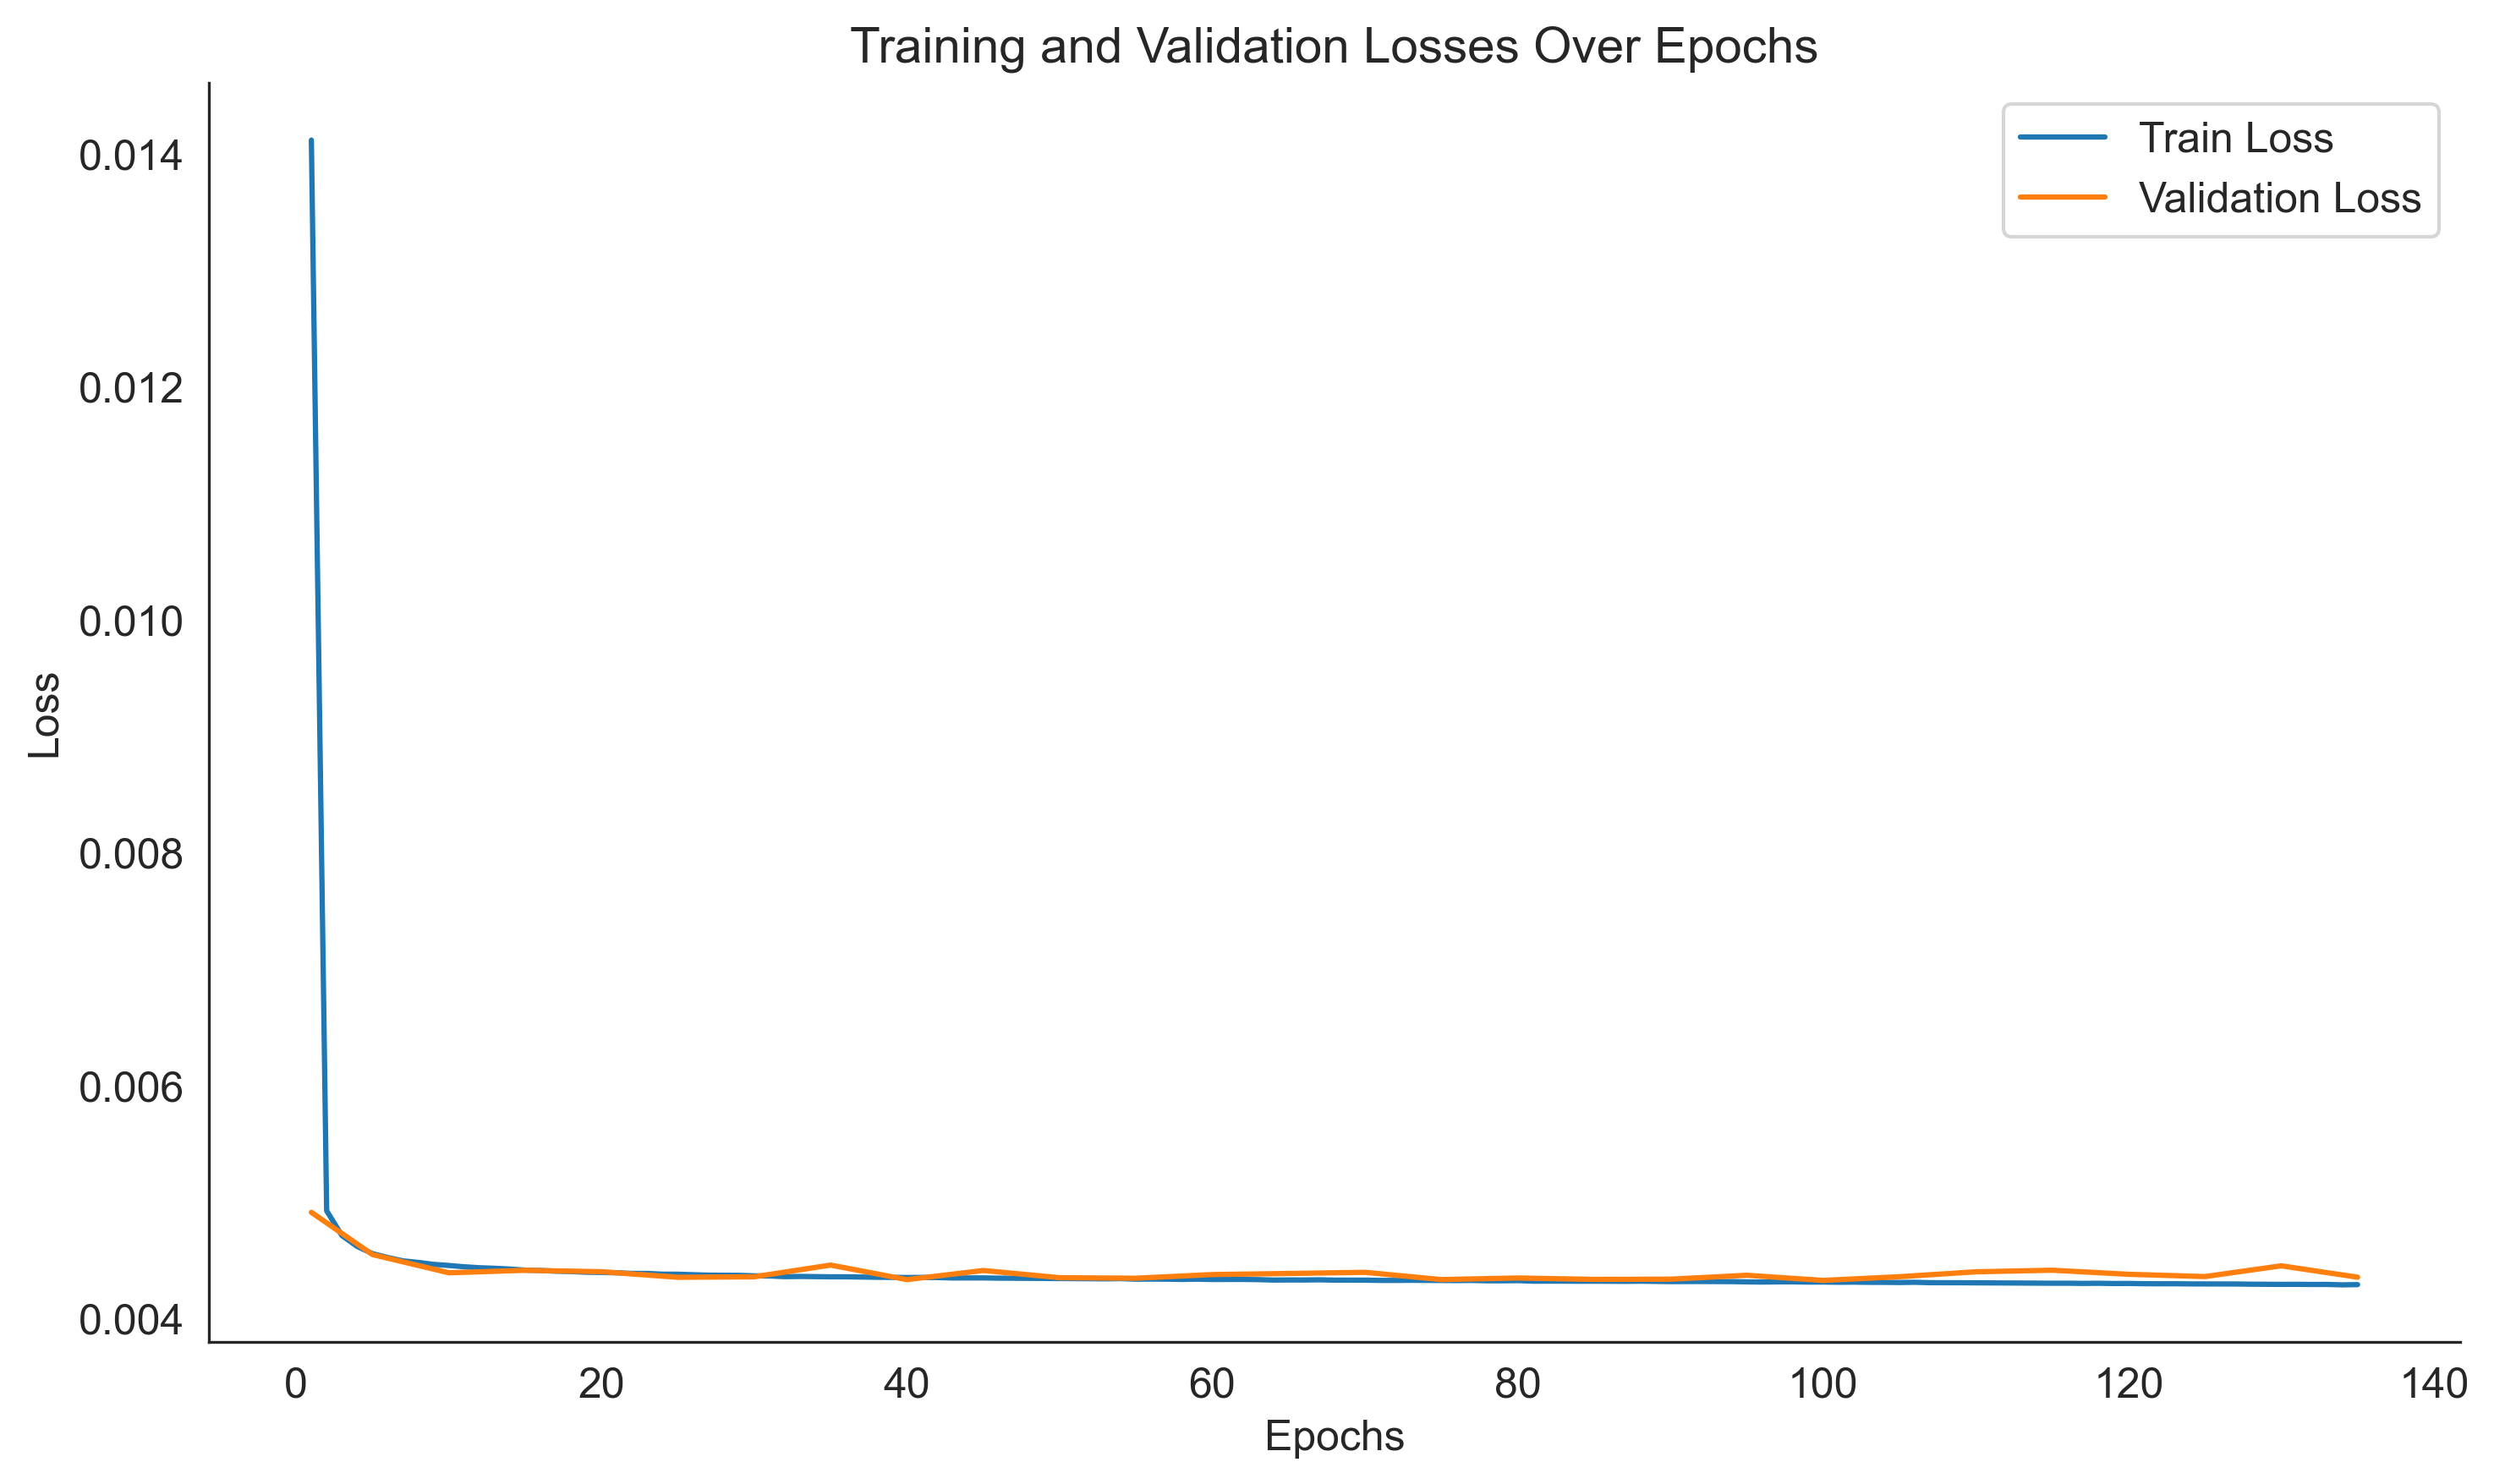
\includegraphics[width=0.90\textwidth]{Thesis/Chapter 3/Figures/fig_train_val_losses_epochs.png}
    \caption{Training and validation \gls{mse} losses over epochs for the final model.}
    \label{fig:train_val_losses_ch3}
\end{subfigure}
\caption{Learning curves for the fitted \gls{dnn}.}
\label{fig:learning_curves_combined_ch3}
\end{figure}

\noindent
Figure~\ref{fig:learning_curves_ch3} presents the learning curves for the
fitted \gls{dnn}. In the left panel, the training \gls{mse} loss drops sharply from
approximately 0.014 at the first epoch to roughly 0.005 by epoch~5, after
which it decreases gradually and stabilises near 0.0043. The validation \gls{mse}
loss tracks the training loss closely throughout, with no visible
divergence between the two curves. The selected epoch $e^{*} = 85$ (green
dashed line) falls in the region where both losses have plateaued. In the
right panel, both training and validation $R^2$ values rise rapidly from
approximately 0.9951 to a plateau near 0.9957, with the gap between them
remaining negligible. Figure~\ref{fig:train_val_losses_ch3} provides a
complementary view: the training loss (blue) exhibits a single spike at
epoch~1, consistent with random weight initialisation, before converging
rapidly, and the validation loss (orange) overlaps with it from epoch~20
onwards. The absence of any sustained divergence confirms stable
convergence without overfitting.

\subsubsection{Actual versus predicted diagnostics}

Two graphical summaries are used to compare observed charges with fitted
predictions.  First, the observed values $y_i$ are plotted directly
against the fitted values $\widehat{y}_i$ with a $45^\circ$ reference
line.  Second, observations are sorted by their observed charge, and the
actual and predicted values are displayed as overlaid curves; a well-fitted
model produces a predicted curve that closely tracks the actual curve across
the full range of the response.  Both diagnostics are produced separately
for the training, validation and test partitions, and together they indicate
whether the fitted model behaves differently in low-, central- and
high-cost regions.

\begin{figure}[H]
\centering
\begin{subfigure}[b]{0.48\textwidth}
    \centering
    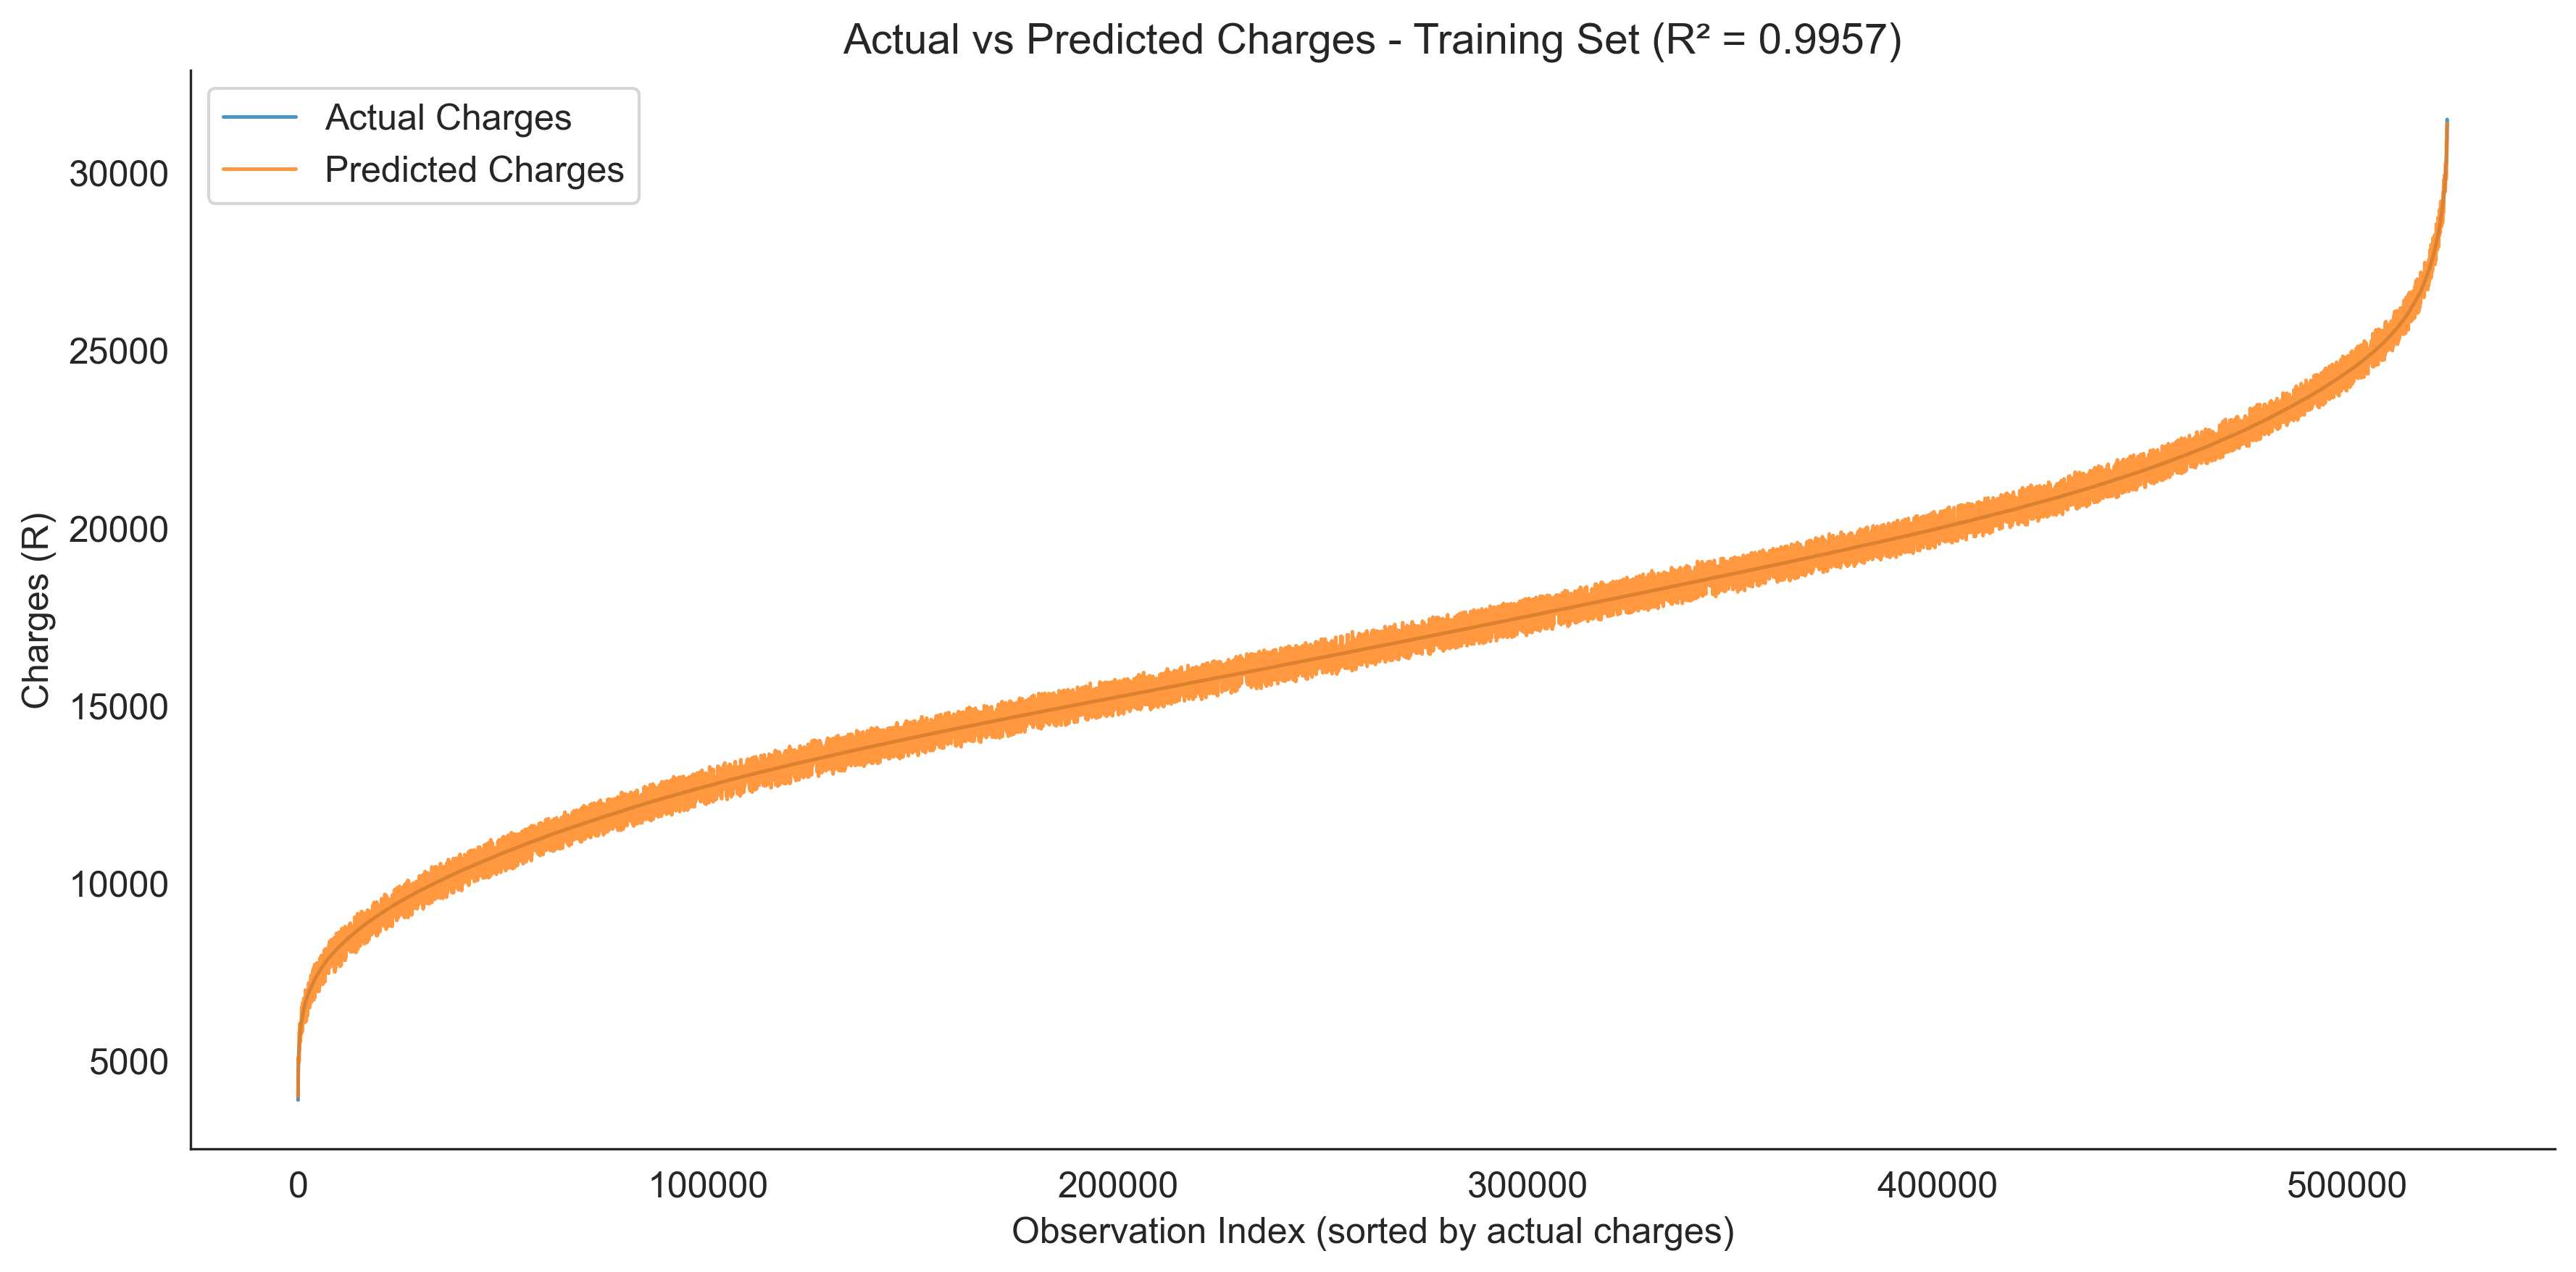
\includegraphics[width=\textwidth]{Thesis/Chapter 3/Figures/fig_actual_vs_predicted_sorted_train.png}
    \caption{Training set ($R^2 = 0.9957$).}
    \label{fig:actual_vs_predicted_train_ch3}
\end{subfigure}
\hfill
\begin{subfigure}[b]{0.48\textwidth}
    \centering
    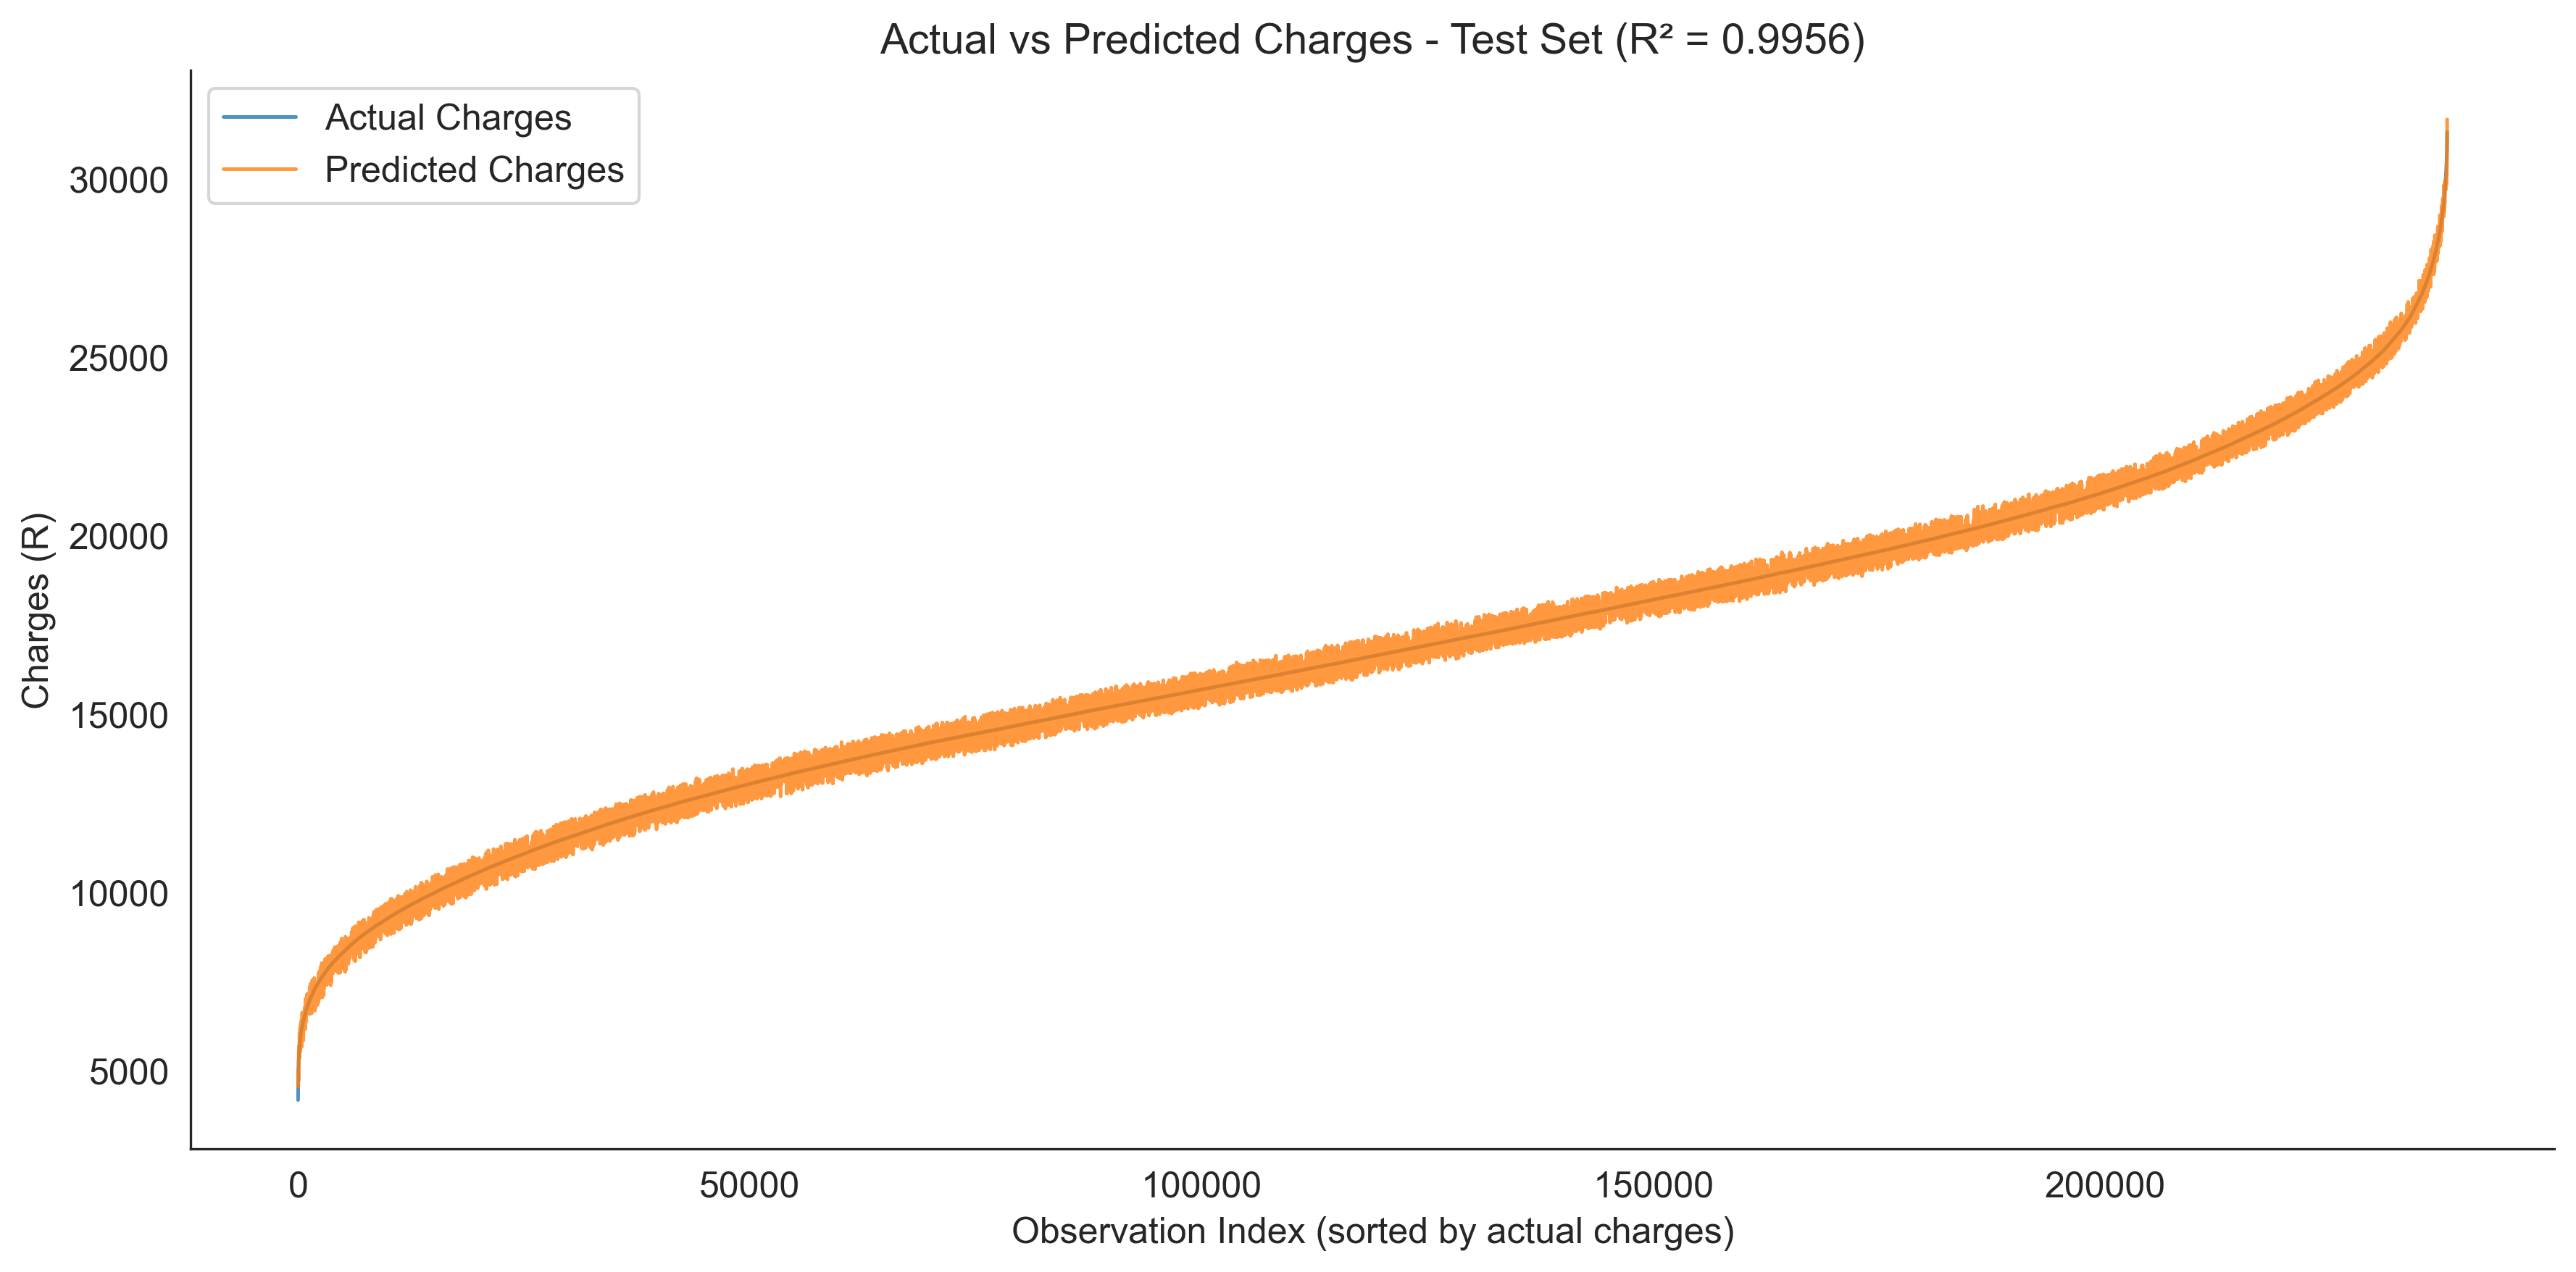
\includegraphics[width=\textwidth]{Thesis/Chapter 3/Figures/fig_actual_vs_predicted_sorted_test.png}
    \caption{Test set ($R^2 = 0.9956$).}
    \label{fig:actual_vs_predicted_test_ch3}
\end{subfigure}
\caption{Sorted actual versus predicted charges on training and test sets.}
\label{fig:actual_vs_predicted_ch3}
\end{figure}

\noindent
Figure~\ref{fig:actual_vs_predicted_ch3} shows the sorted actual versus
predicted charges on both partitions. In the training set
(Figure~\ref{fig:actual_vs_predicted_train_ch3}), the predicted line
(orange) tracks the actual line (blue) so closely that the two are nearly
indistinguishable across the full range of the response, from approximately
R4\,000 at the lower end to R32\,000 at the upper end. A modest increase
in prediction scatter is visible in the upper tail above R25\,000, but the
deviations remain small relative to the response scale. The test set
(Figure~\ref{fig:actual_vs_predicted_test_ch3}) displays a virtually
identical pattern. The negligible drop from training $R^2 = 0.9957$ to test
$R^2 = 0.9956$ confirms that the model generalises to unseen observations
without meaningful performance degradation.

\begin{figure}[H]
\centering
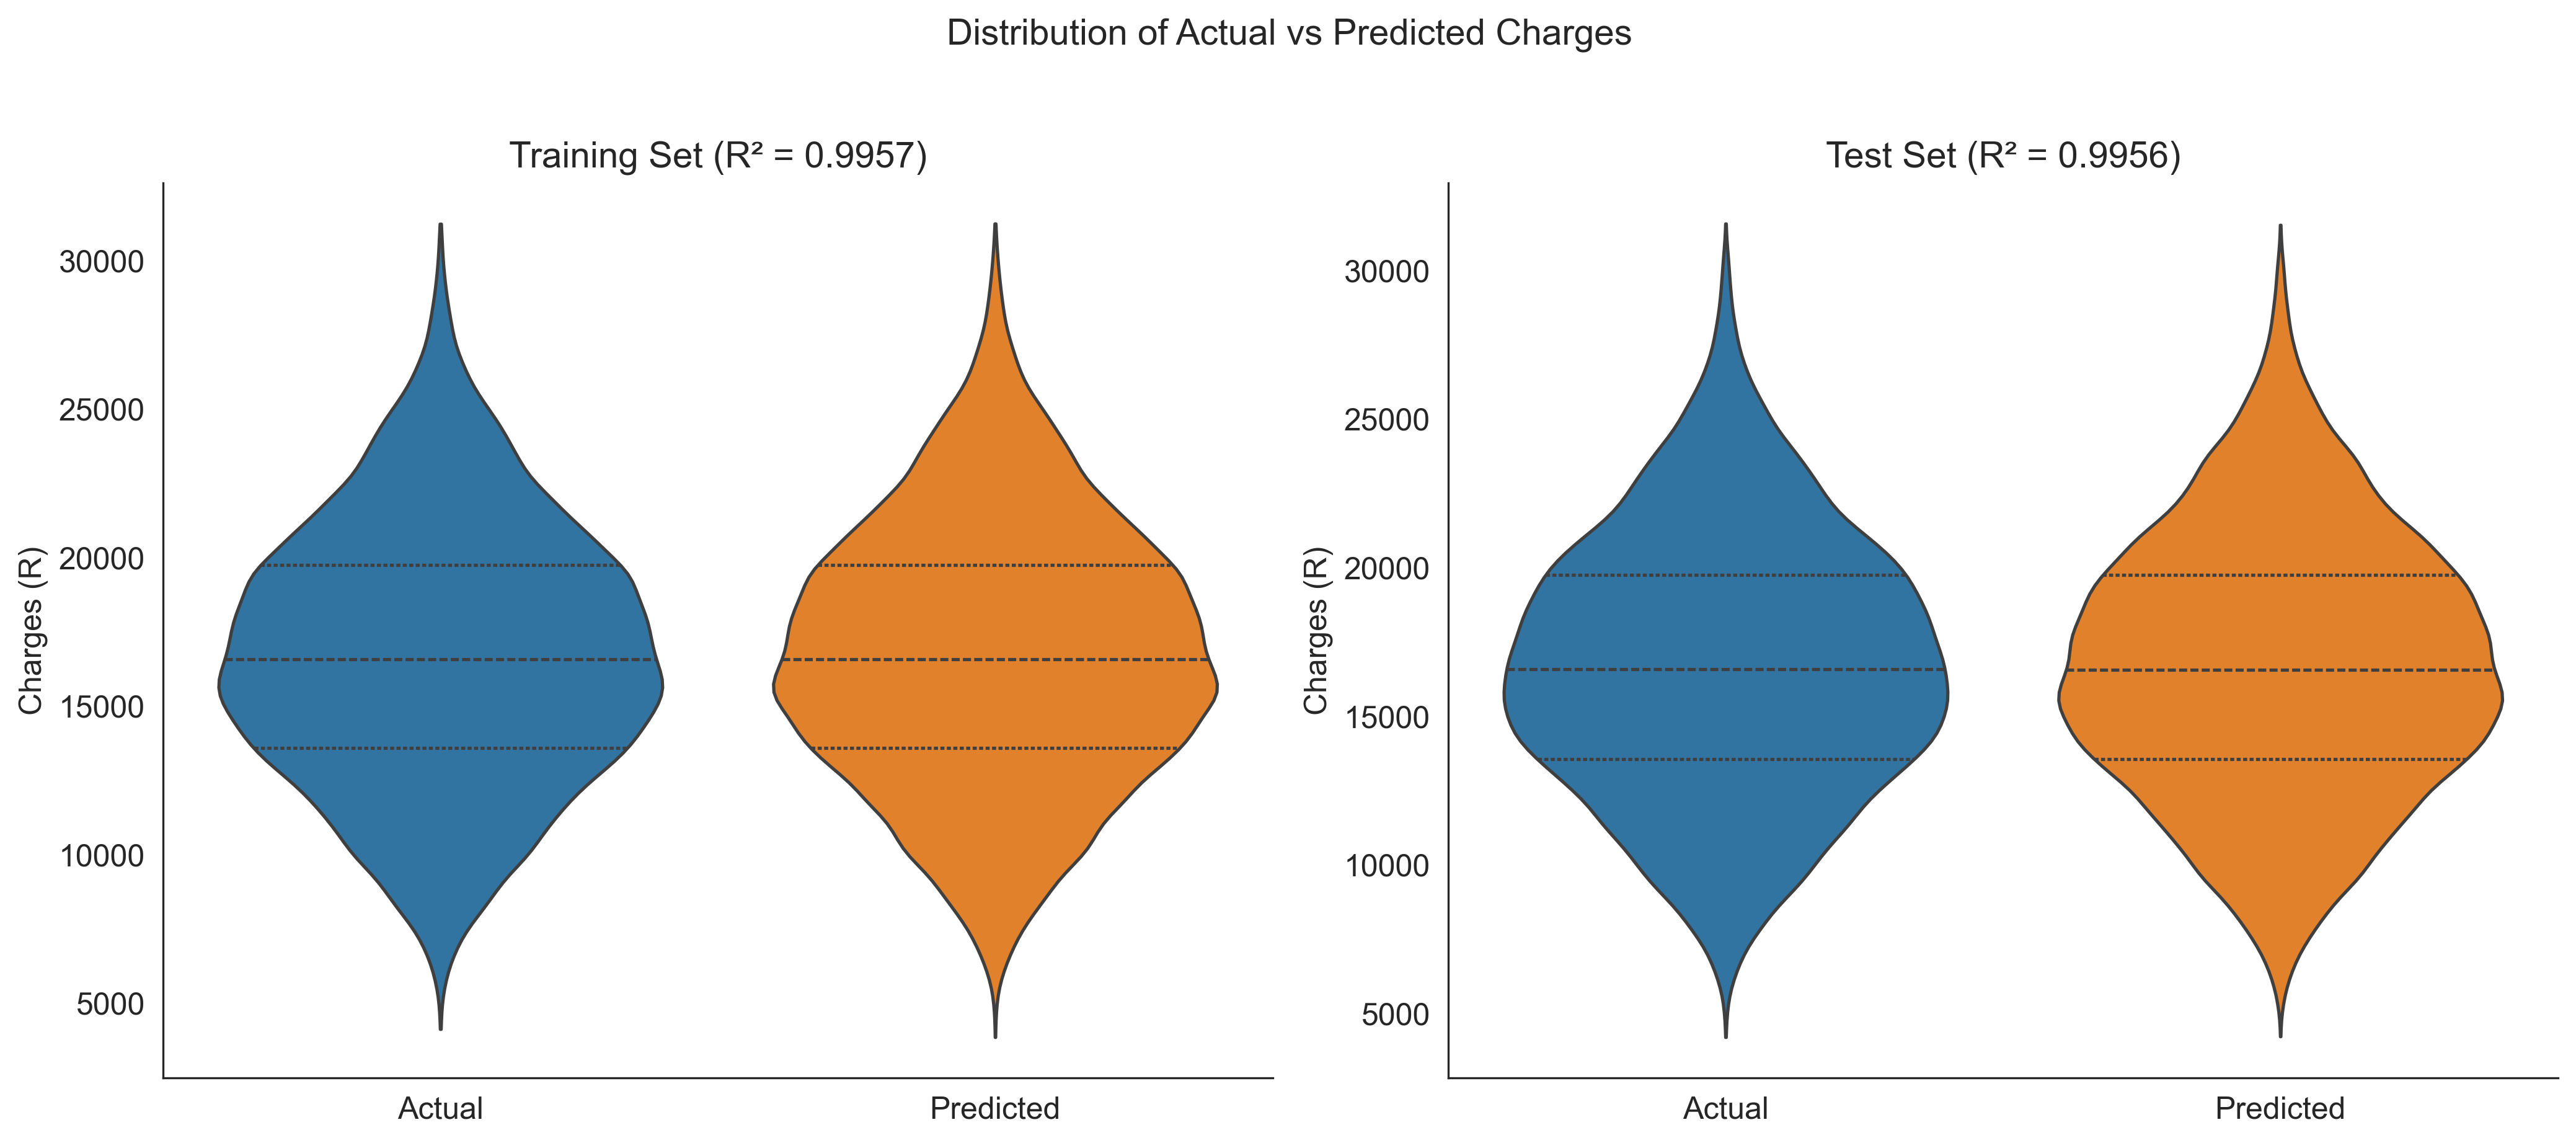
\includegraphics[width=0.90\textwidth]{Thesis/Chapter 3/Figures/fig_violin_actual_vs_predicted.png}
\caption{Violin plots of actual versus predicted charges on training and test sets.}
\label{fig:violin_actual_vs_predicted_ch3}
\end{figure}

\noindent
Figure~\ref{fig:violin_actual_vs_predicted_ch3} compares the distributional
profiles of actual and predicted charges on both partitions. In the
training set (left panel, $R^2 = 0.9957$), the actual (blue) and predicted
(orange) violins exhibit closely matching shapes: both are unimodal with
the bulk of density concentrated between approximately R10\,000 and
R25\,000, and the dashed median lines fall at approximately the same level
near R16\,700. The predicted violin is marginally narrower at the extreme
tails, indicating that the \gls{dnn} compresses the most extreme values slightly,
which is consistent with the smoothing behaviour of a regression model. The
test set (right panel, $R^2 = 0.9956$) displays the same pattern, with the
actual and predicted distributions virtually mirroring each other. The
consistency between training and test panels confirms that the model's
distributional calibration is preserved on unseen data.

\subsubsection{Residual diagnostics}

Residual diagnostics examine whether prediction errors contain systematic
structure.  Using the residuals defined in
equation~\eqref{eq:residual_definition_ch3}, the following plots are
produced:
\begin{enumerate}
    \item residuals versus fitted values, to detect systematic bias or
          changes in spread;
    \item a residual histogram, to assess the empirical shape and centring
          of the prediction errors;
    \item a $Q\text{-}Q$ plot of standardised residuals, to inspect tail
          behaviour;
    \item residuals versus observation index, to identify possible ordering
          or sequential patterns;
    \item residual distribution comparisons across the training, validation
          and test partitions.
\end{enumerate}
The \gls{dnn} does not require normally distributed residuals; these checks
are purely descriptive.  The fitted residuals are also retained for the
residual-augmented \gls{mc} sensitivity analysis described later.

\begin{figure}[H]
\centering
\begin{subfigure}[b]{\textwidth}
    \centering
    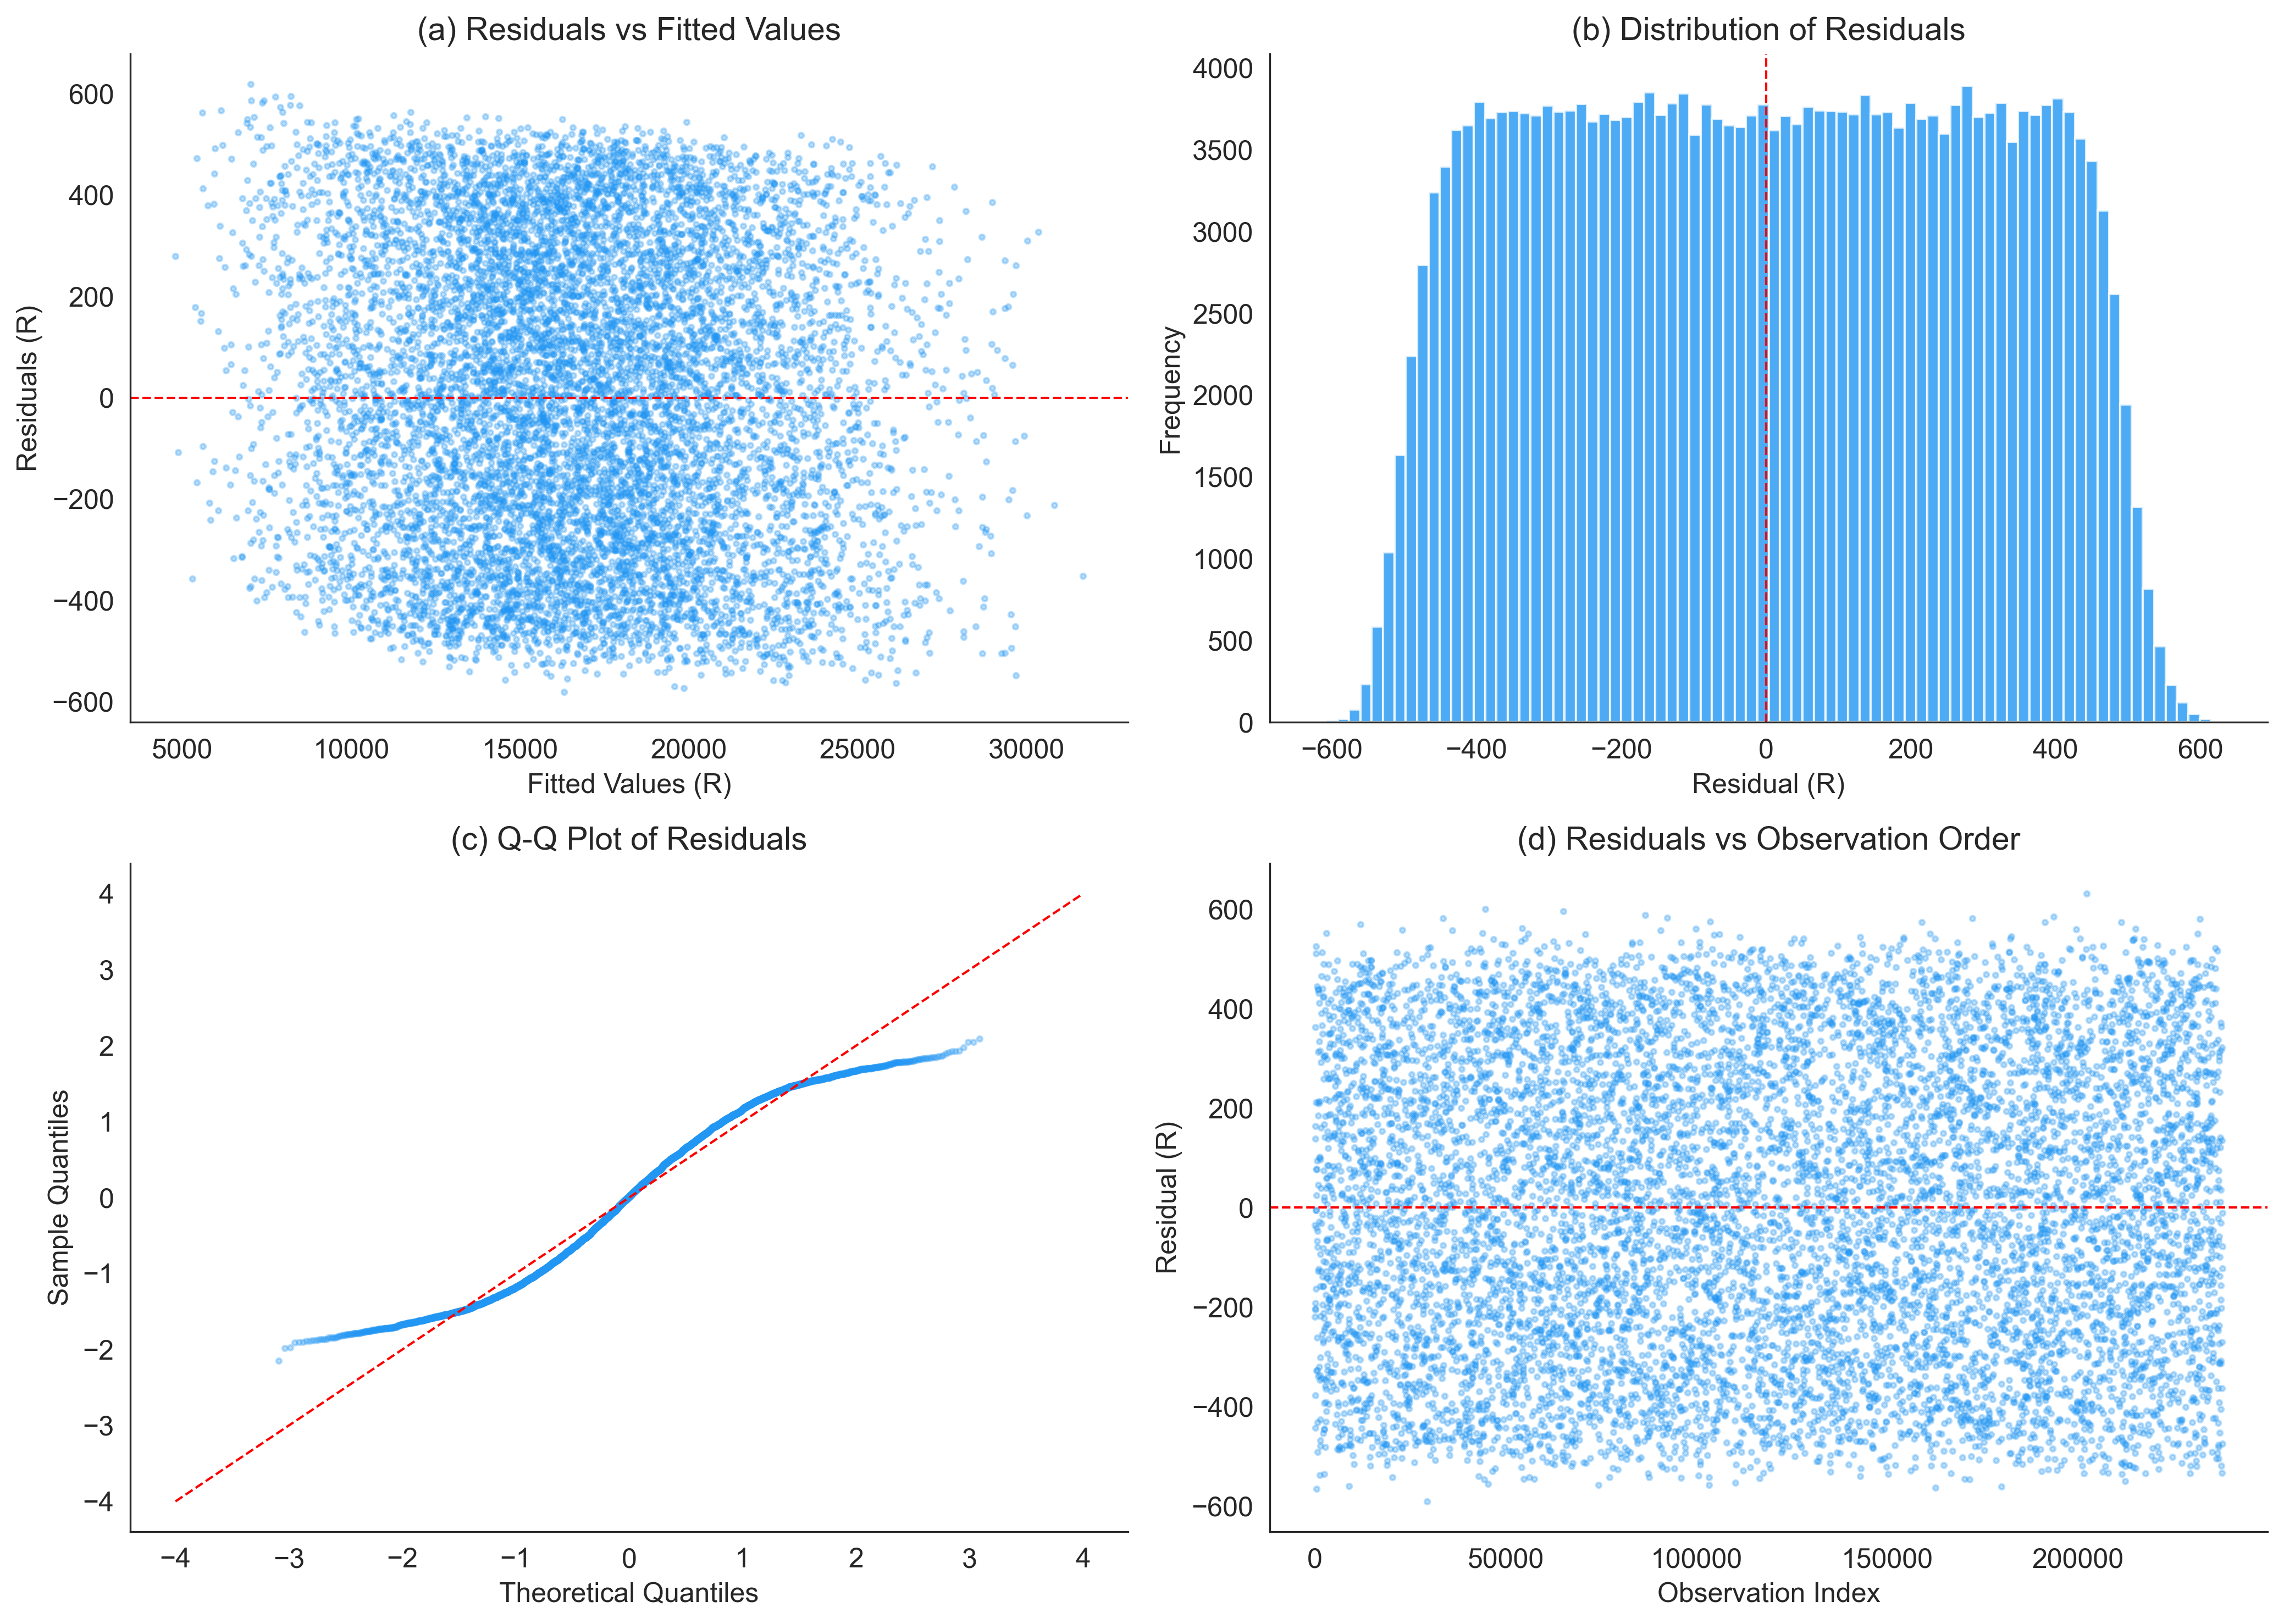
\includegraphics[width=0.90\textwidth]{Thesis/Chapter 3/Figures/fig_residual_diagnostics.png}
    \caption{Residual diagnostic panels for the fitted \gls{dnn}.}
    \label{fig:residual_diagnostics_ch3}
\end{subfigure}

\vspace{0.4cm}

\begin{subfigure}[b]{0.55\textwidth}
    \centering
    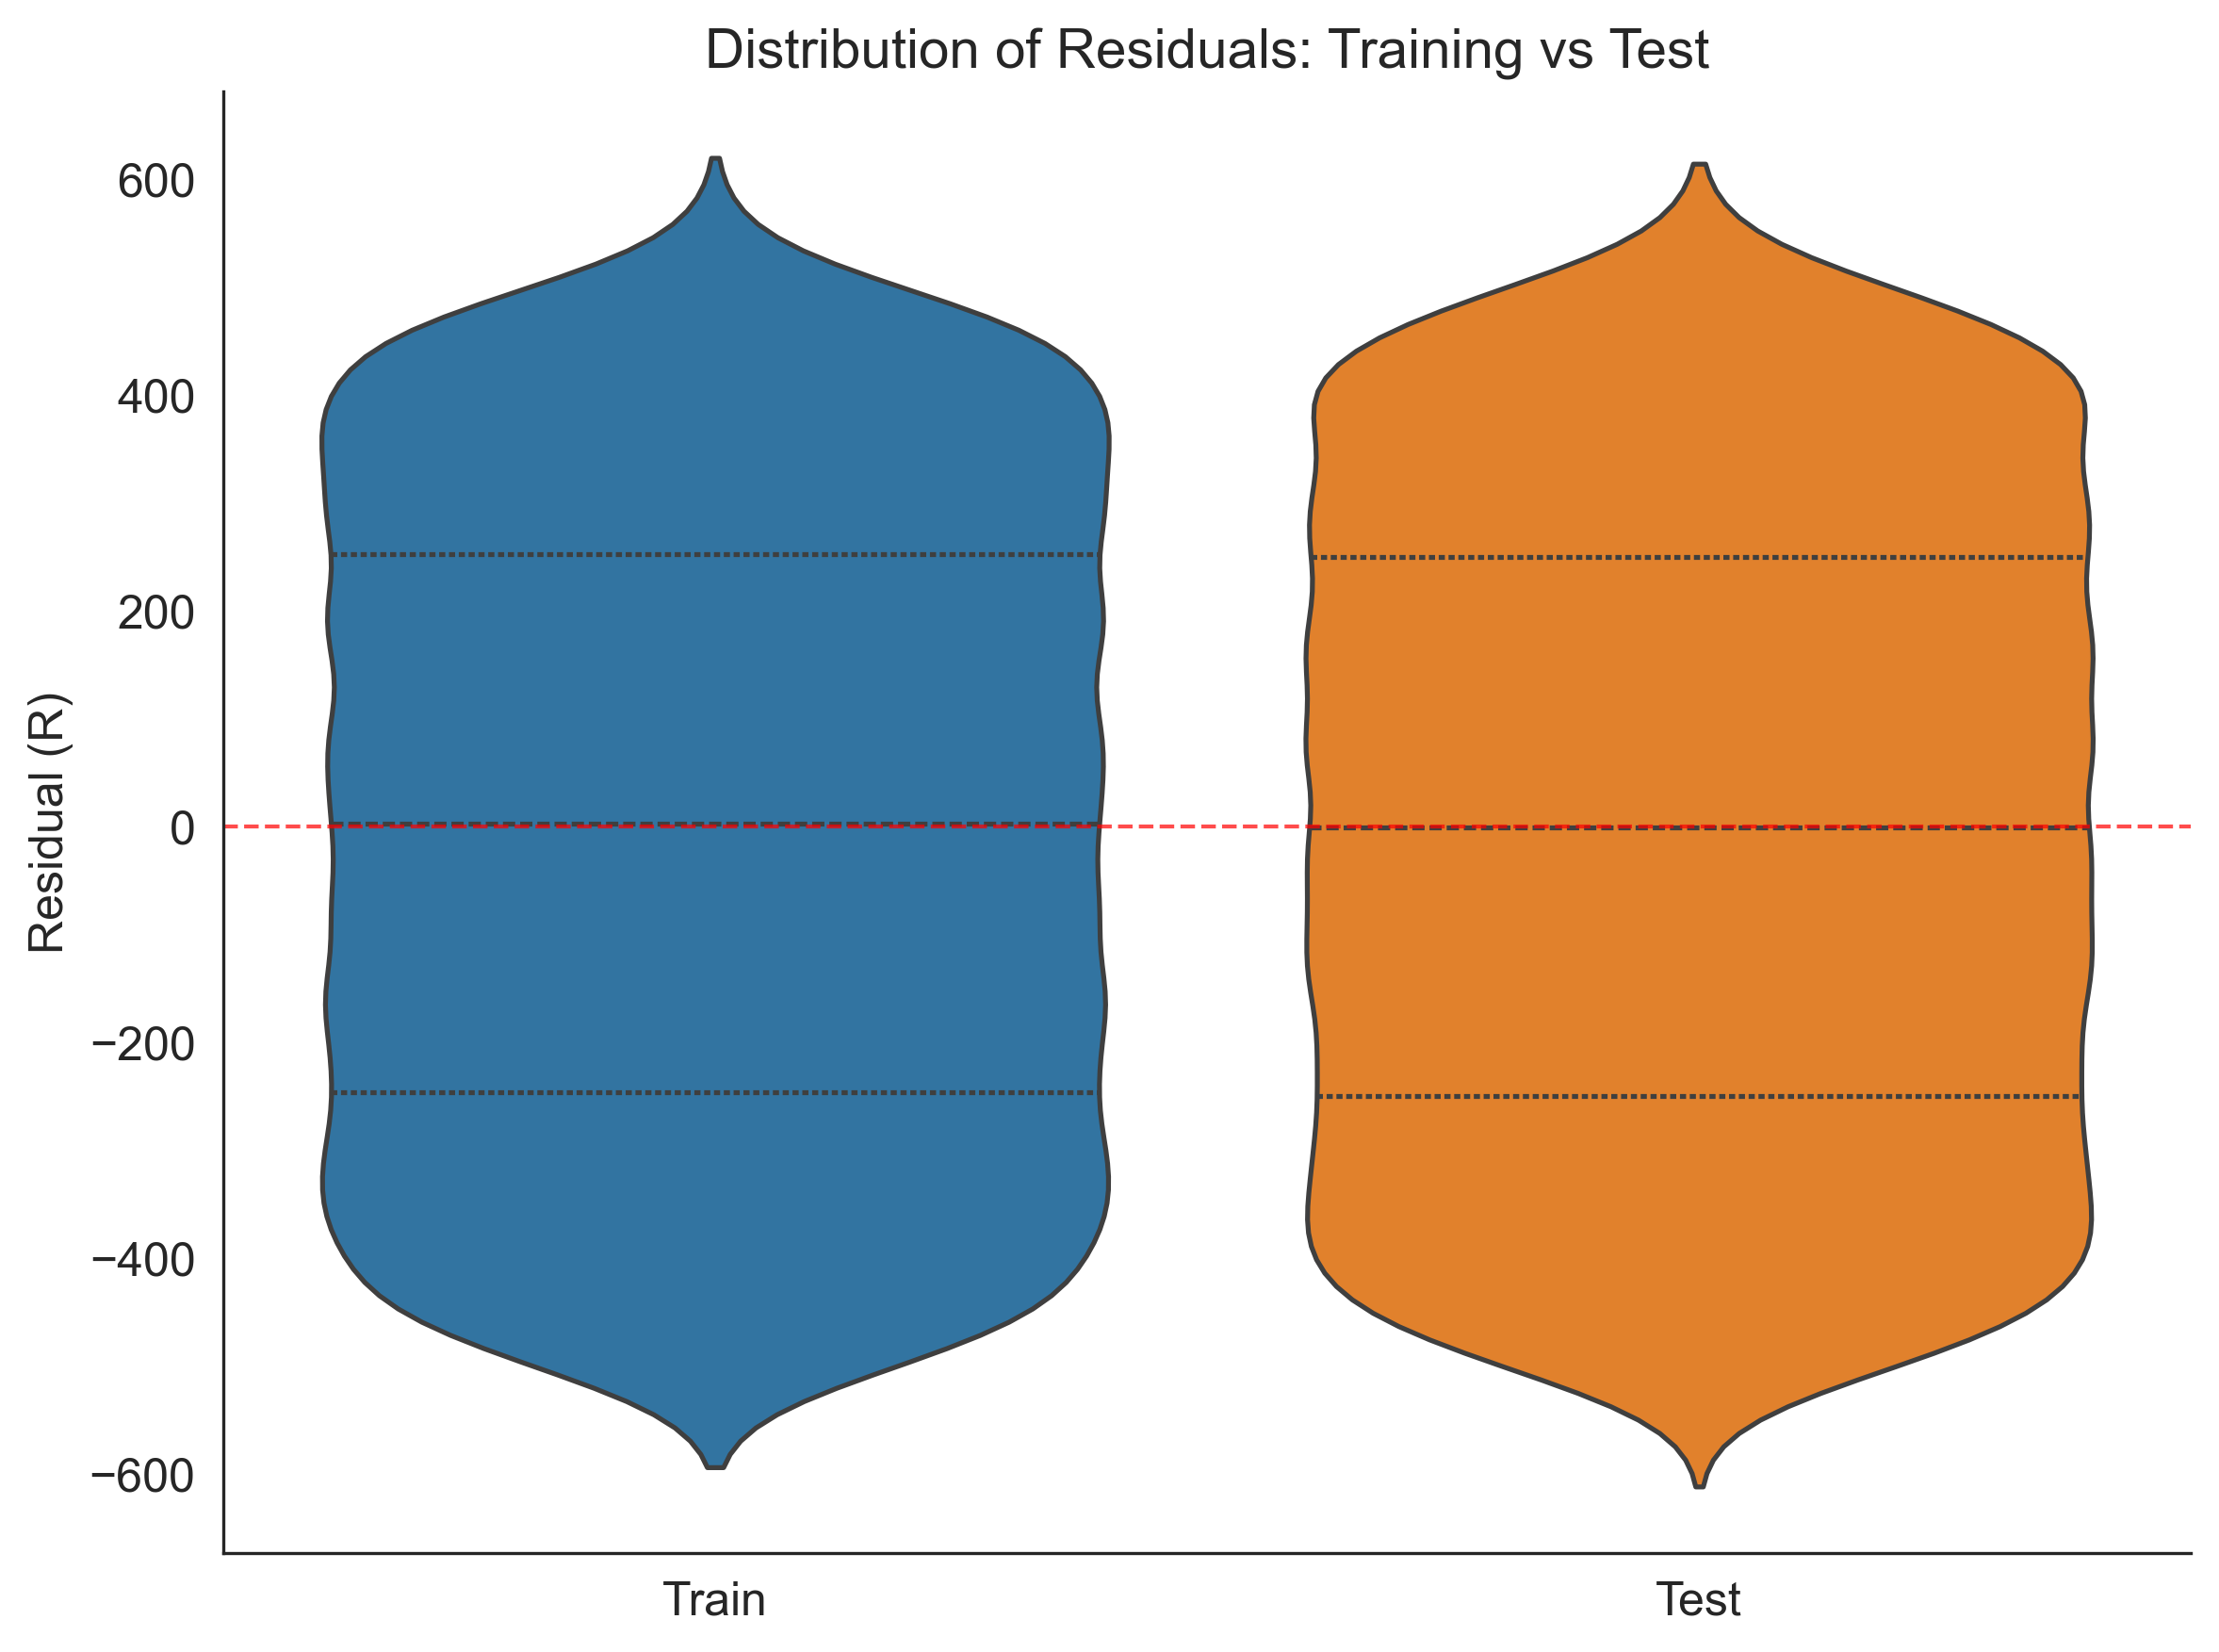
\includegraphics[width=\textwidth]{Thesis/Chapter 3/Figures/fig_violin_residuals.png}
    \caption{Violin plots of residuals on the training and test sets.}
    \label{fig:violin_residuals_ch3}
\end{subfigure}
\caption{Residual diagnostics for the fitted \gls{dnn}.}
\label{fig:residual_analysis_ch3}
\end{figure}

\noindent
Figure~\ref{fig:residual_diagnostics_ch3} presents the four residual
diagnostic panels for the test set. Panel~(a) shows residuals versus fitted
values: the residuals are centred at zero across the full range of fitted
charges (approximately R5\,000 to R30\,000), with no visible funnel shape
or systematic trend. The residual magnitudes range from approximately
$-600$ to $+600$, which is small relative to the response scale.
Panel~(b) displays the residual histogram, which is symmetric and centred
at zero but distinctly non-Gaussian: the distribution is platykurtic and
plateau-shaped, with probability spread nearly evenly across a bounded
interval and hard cutoffs near $\pm 600$ rather than smoothly decaying
tails. Panel~(c) shows the Q-Q plot of standardised residuals. The central
portion follows the theoretical reference line, while both tails bend
markedly away from it, confirming that the residual distribution is
bounded, with far lighter tails than a Gaussian distribution. This
bounded, near-uniform residual shape is the fingerprint of the benchmark's
data-generating process: the response is produced by a deterministic cost
formula with a bounded random perturbation, which explains both the hard
residual cutoffs and the near-ceiling $R^2$ values observed on every
partition. Consequently, the accuracy figures reported in this study
characterise how well the network recovers an algorithmic generating
formula, and no claim is made that these specific figures transfer to real
insurance portfolios (see the delimitations in
Section~\ref{sec:scope_delimitations}). The non-Gaussian residual shape is
not itself a concern for the \gls{dnn}, which does not assume normality of
residuals. Panel~(d) plots
residuals against observation index: the points are scattered randomly
around zero with no discernible sequential pattern.
Figure~\ref{fig:violin_residuals_ch3} compares the residual distributions
across partitions. Both the training and test violins are centred at zero
and are nearly identical in width, spread and symmetry, confirming that the
residual error does not systematically differ between the training and test
data and that the fitted \gls{dnn} does not overfit the training partition.

\subsubsection{Principal component structural diagnostics}
\label{sec:pca_structural_diagnostics}

\gls{pca} is employed as a structural diagnostic of the standardised,
model-ready input space.  It is not used for dimension reduction, and no
predictors are removed on the basis of the principal components.  The
purpose is twofold: to assess whether the data partition preserves the
structure of the input space, and to check whether the fitted predictions
reproduce the dominant target pattern when displayed on the same
low-dimensional projection.

Let
$\widetilde{\mathbf{X}} \in \mathbb{R}^{n_{\mathrm{train}} \times p}$
denote the column-standardised training input matrix ($p = 22$).  The
sample covariance matrix is
\begin{equation}
    \mathbf{S}
    = \frac{1}{n_{\mathrm{train}}-1}\,
      \widetilde{\mathbf{X}}^{\!\top}\widetilde{\mathbf{X}} .
    \label{eq:pca_covariance_matrix}
\end{equation}
\equationlistentry{PCA sample covariance matrix}
Its spectral decomposition is
\begin{equation}
    \mathbf{S}
    = \mathbf{W}\boldsymbol{\Lambda}\mathbf{W}^{\!\top},
    \qquad
    \boldsymbol{\Lambda}
    = \operatorname{diag}(\lambda_1,\dots,\lambda_p),
    \qquad
    \lambda_1 \geq \lambda_2 \geq \cdots \geq \lambda_p \geq 0 ,
    \label{eq:pca_eigendecomposition}
\end{equation}
\equationlistentry{PCA eigenvalue decomposition}
where $\mathbf{W} = [\mathbf{w}_1 \cdots \mathbf{w}_p]$ contains the
principal loading vectors.  The score of observation $i$ on component
$k$ is
\begin{equation}
    z_{ik} = \widetilde{\mathbf{x}}_i^{\!\top}\mathbf{w}_k,
    \qquad k = 1,\dots,p .
    \label{eq:pca_scores}
\end{equation}
\equationlistentry{PCA principal component scores}
The \gls{pca} decomposition is computed from the training partition only; the
resulting eigenvectors are then used to project the validation and test
observations, so that all sets are displayed in a common coordinate system.
The first two principal components provide the two-dimensional diagnostic
projection.

Two \gls{pca} comparisons are performed.  First, the training, validation and test
point clouds are overlaid; similar structure across partitions supports the
view that the data split has not introduced a major structural shift.
Second, the same \gls{pca} coordinates are coloured by observed charges and by
fitted predictions; similar colour gradients indicate that the fitted
\gls{dnn} has captured the dominant target structure visible in the input
space.

The loading vectors are inspected to verify that the first two principal
components are not driven by a single variable and that they account for a
moderate share of the total variance, so that the diagnostic is not
dominated by one narrow direction \citep{hastie2009elements}.  This
inspection is descriptive and is not used to modify the fitted model.

\begin{figure}[H]
\centering
\begin{subfigure}[b]{0.48\textwidth}
    \centering
    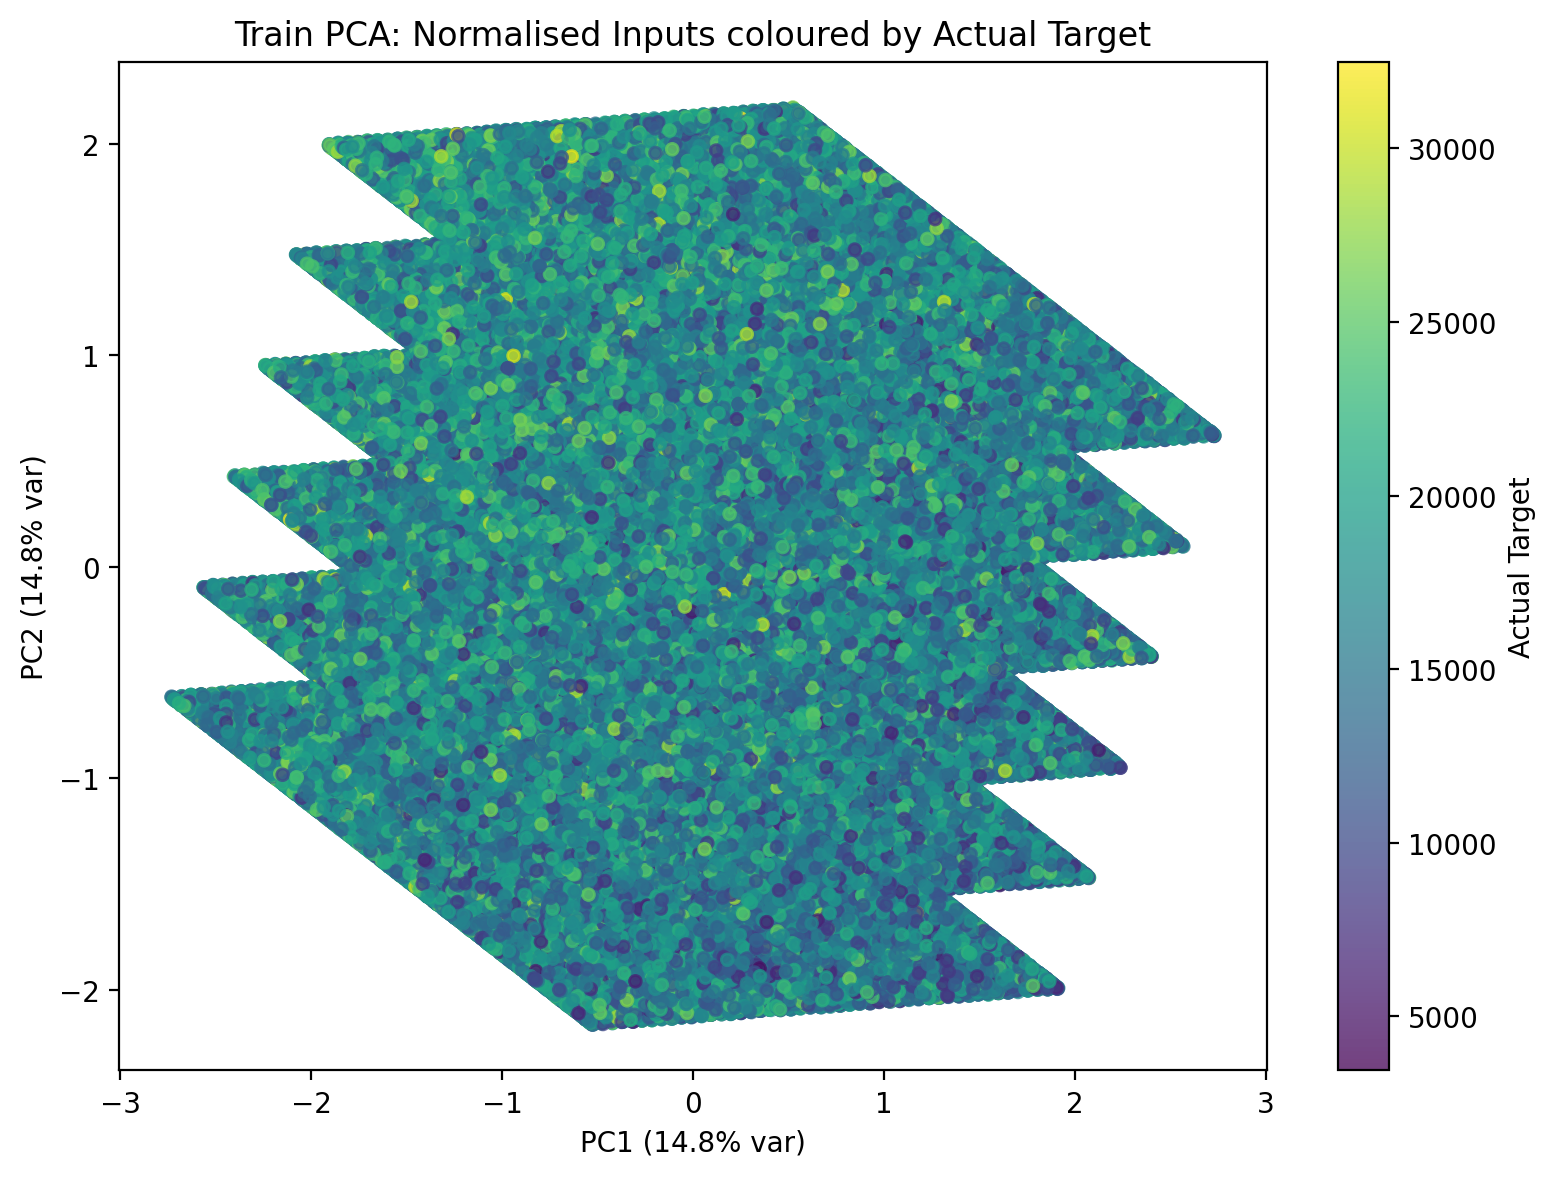
\includegraphics[width=\textwidth]{Thesis/Chapter 3/Figures/fig_sml_pca_train_actual.png}
    \caption{Training set, actual charges.}
    \label{fig:pca_train_actual_ch3}
\end{subfigure}
\hfill
\begin{subfigure}[b]{0.48\textwidth}
    \centering
    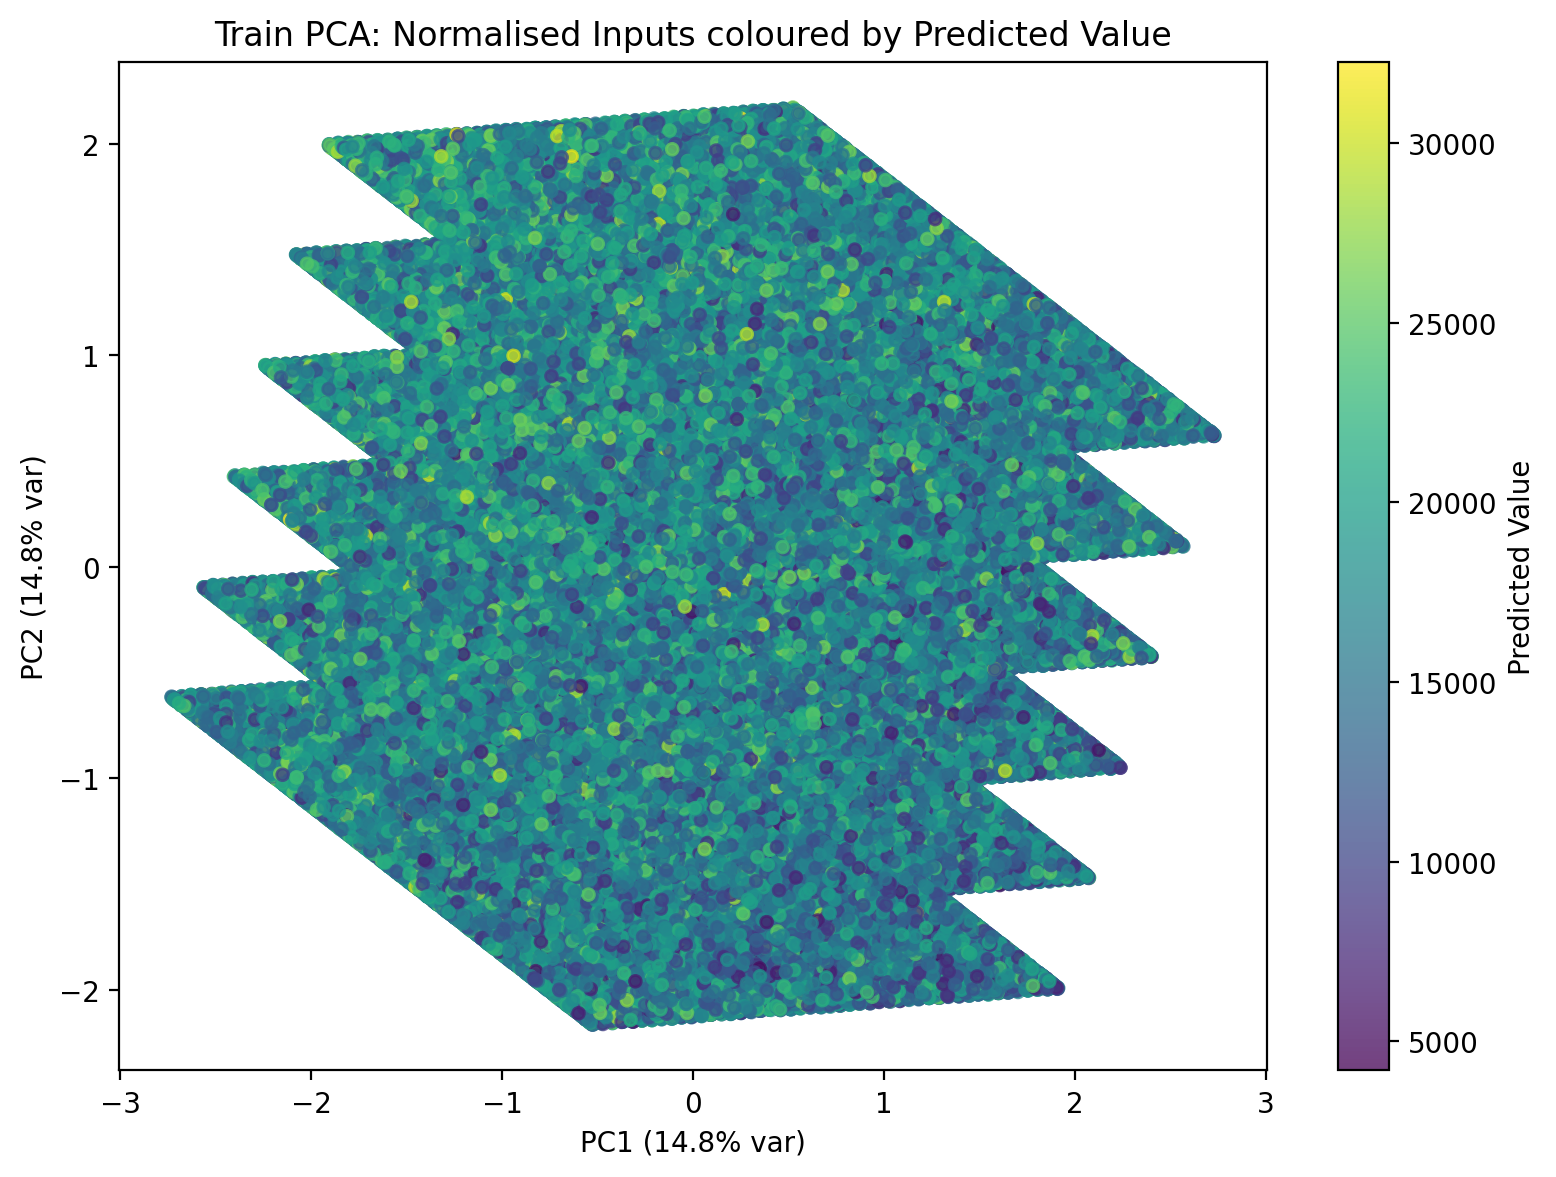
\includegraphics[width=\textwidth]{Thesis/Chapter 3/Figures/fig_sml_pca_train_predicted.png}
    \caption{Training set, predicted charges.}
    \label{fig:pca_train_predicted_ch3}
\end{subfigure}

\vspace{0.4cm}

\begin{subfigure}[b]{0.48\textwidth}
    \centering
    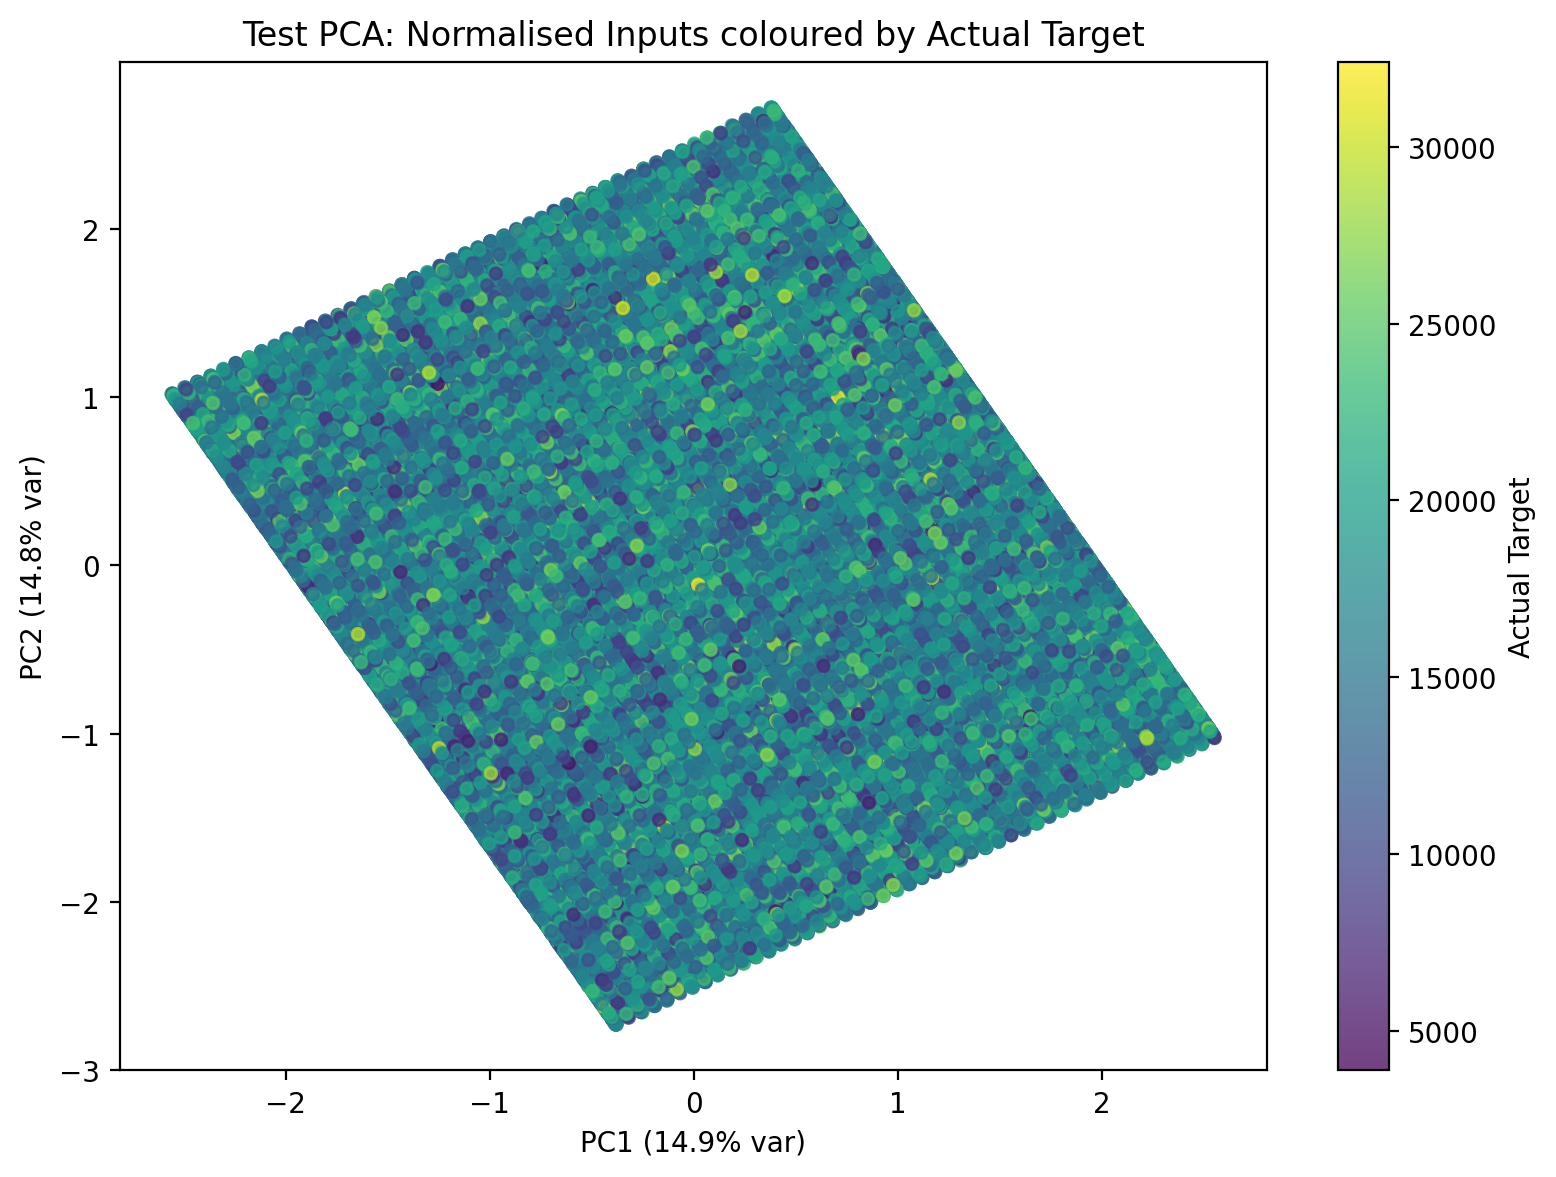
\includegraphics[width=\textwidth]{Thesis/Chapter 3/Figures/fig_sml_pca_test_actual.png}
    \caption{Test set, actual charges.}
    \label{fig:pca_test_actual_ch3}
\end{subfigure}
\hfill
\begin{subfigure}[b]{0.48\textwidth}
    \centering
    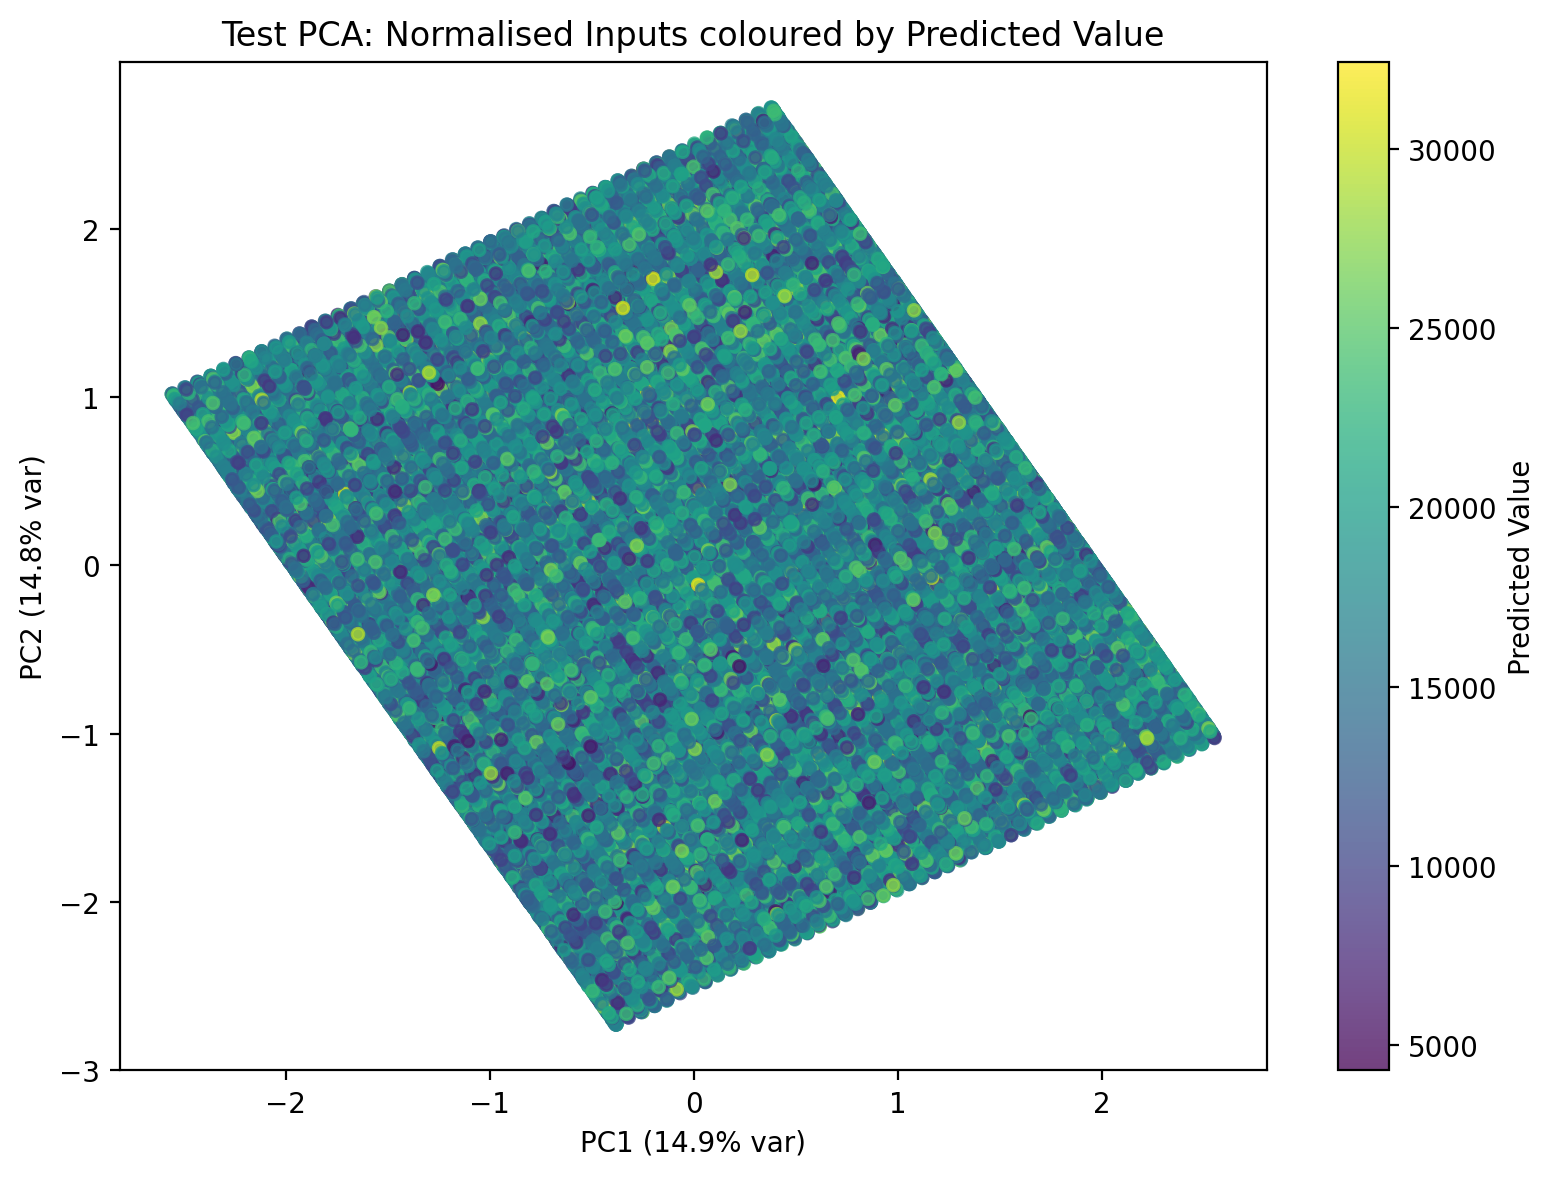
\includegraphics[width=\textwidth]{Thesis/Chapter 3/Figures/fig_sml_pca_test_predicted.png}
    \caption{Test set, predicted charges.}
    \label{fig:pca_test_predicted_ch3}
\end{subfigure}
\caption{\Gls{pca} projections coloured by actual and predicted charges on training and test sets.}
\label{fig:pca_diagnostics_ch3}
\end{figure}

\noindent
Figure~\ref{fig:pca_diagnostics_ch3} displays the \gls{pca} diagnostic scatter
plots. In the training set
(Figures~\ref{fig:pca_train_actual_ch3}
and~\ref{fig:pca_train_predicted_ch3}), the first two principal components
each explain approximately 14.8\% of the total variance. The point cloud
exhibits a layered structure with several horizontal shelves, reflecting the
discrete levels of the encoded categorical predictors projected onto the PC
axes. The colour gradient, representing charges from approximately R5\,000
(purple) to R30\,000 (yellow), is broadly mixed across the point cloud,
with higher charges (yellow-green) tending to appear at specific regions
within the layered structure. The predicted-target colouring
(Figure~\ref{fig:pca_train_predicted_ch3}) is virtually indistinguishable
from the actual-target version, confirming that the fitted \gls{dnn} has captured
the dominant target structure visible in the first two principal component
directions. The test set
(Figures~\ref{fig:pca_test_actual_ch3}
and~\ref{fig:pca_test_predicted_ch3}) shows the same point-cloud shape and
colour distribution as the training set (PC1: 14.9\%, PC2: 14.8\%),
and the actual and predicted colourings again match closely. This
consistency across partitions and between actual and predicted targets
jointly satisfies both the partition consistency and model capture
diagnostic criteria.

\begin{figure}[H]
\centering
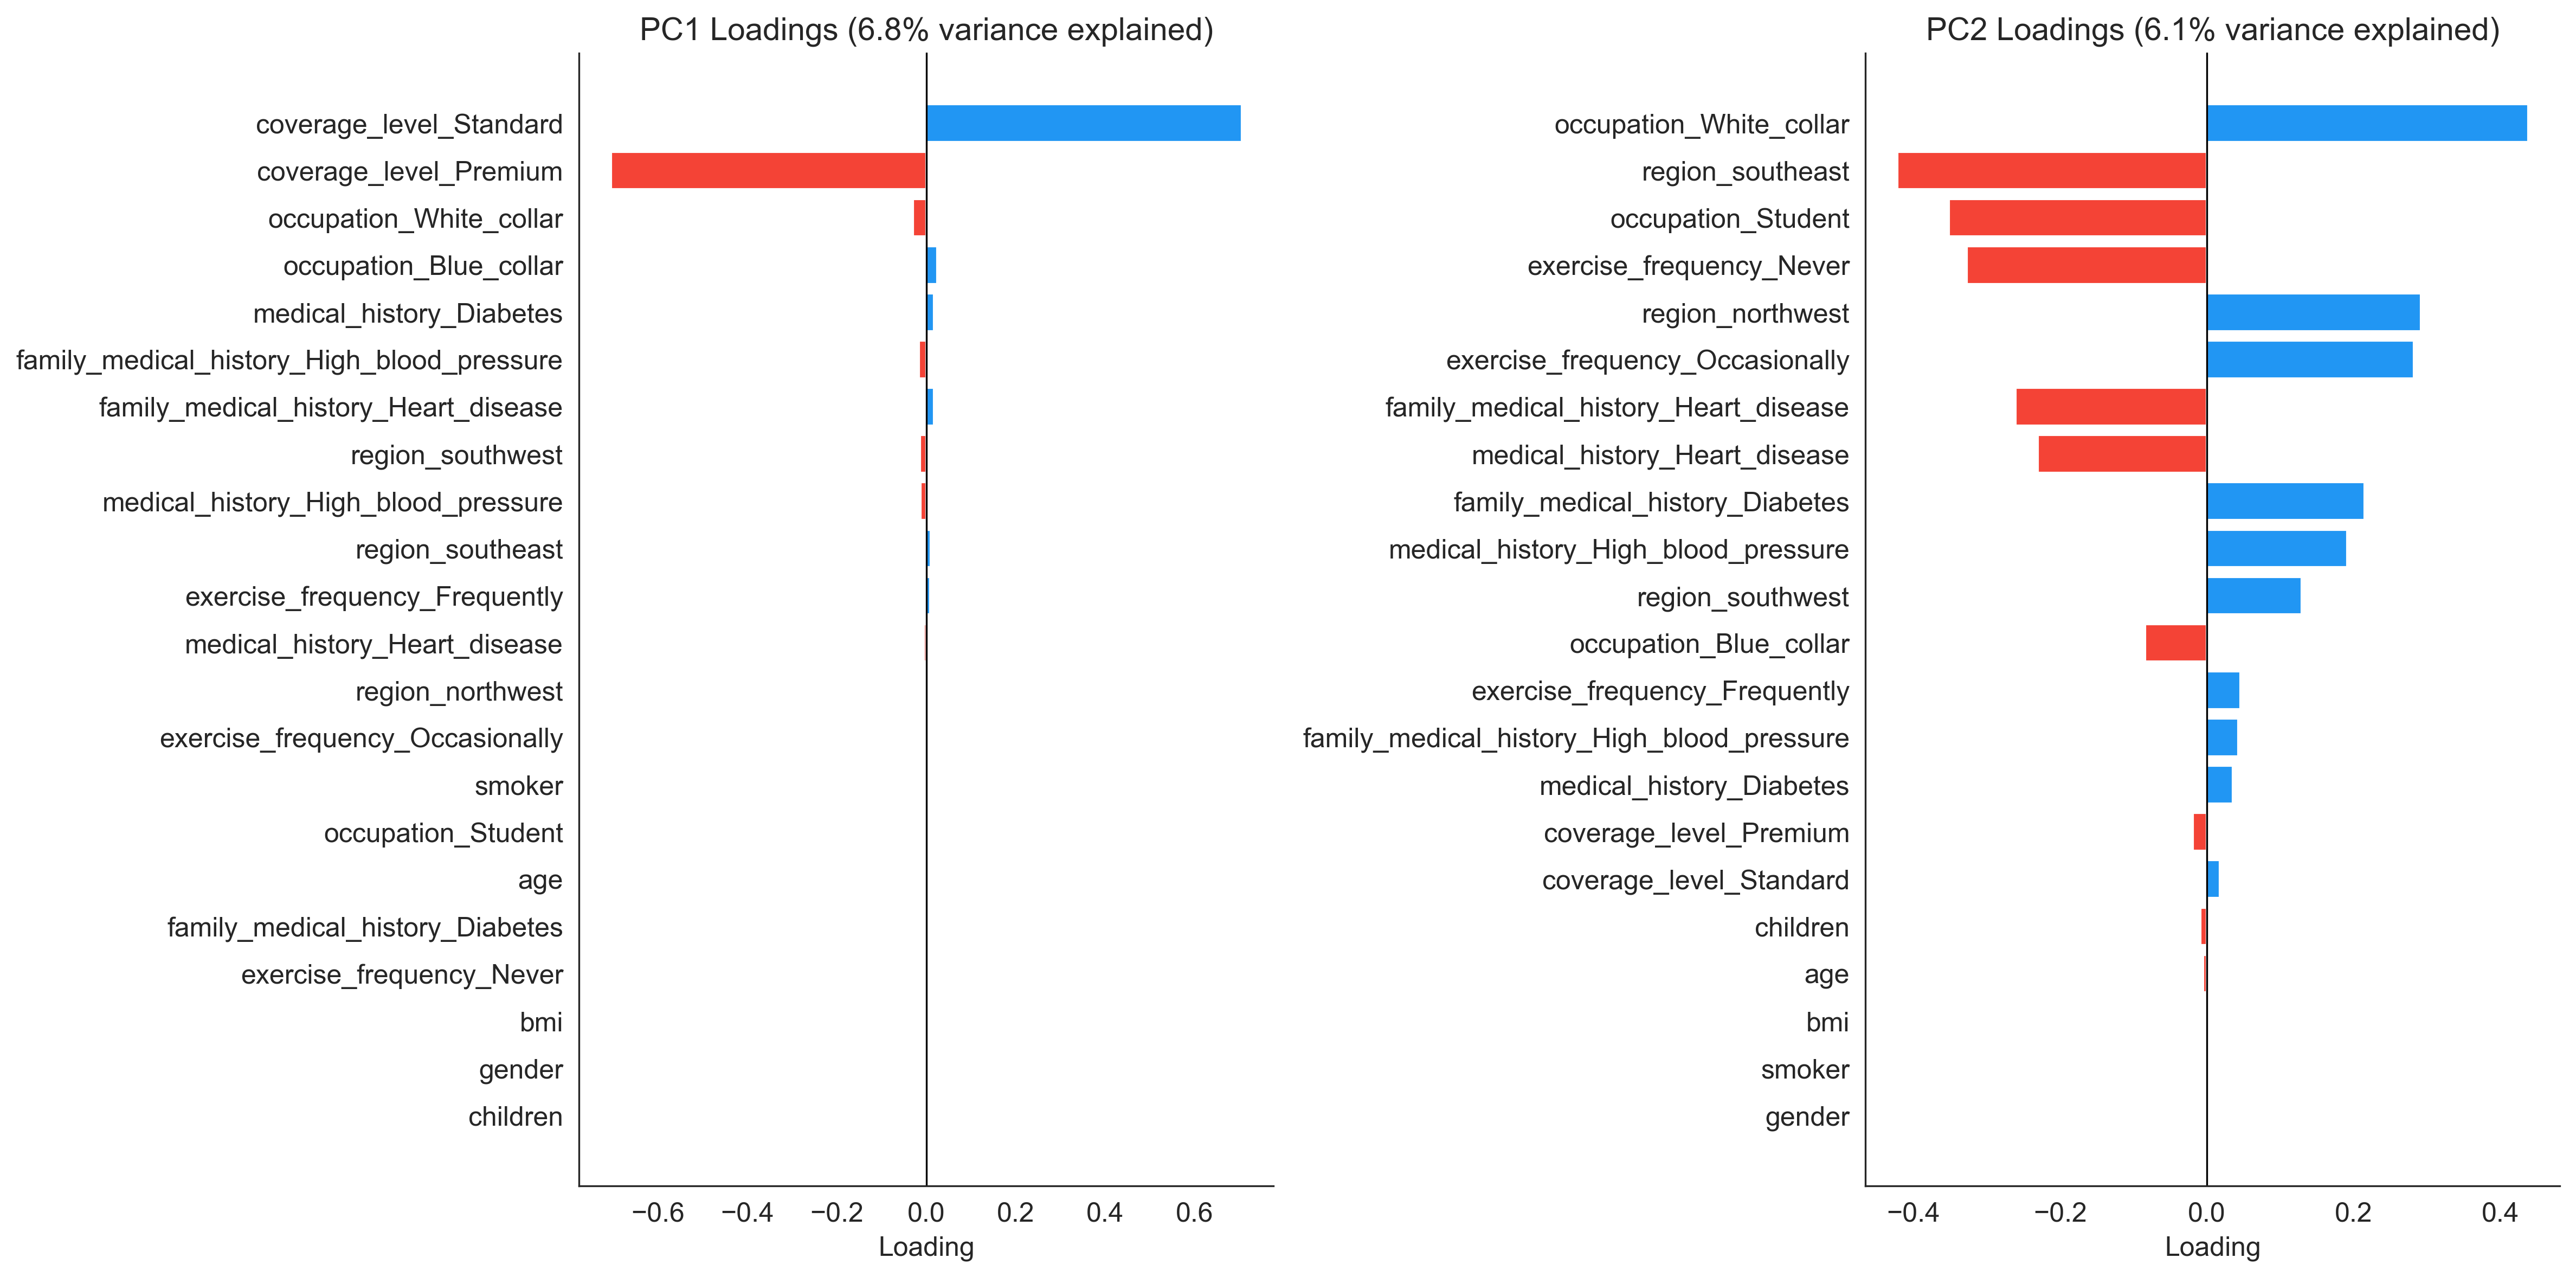
\includegraphics[width=0.90\textwidth]{Thesis/Chapter 3/Figures/fig_pca_loadings.png}
\caption{\Gls{pca} loading vectors for all 22 encoded predictors.}
\label{fig:pca_loadings_ch3}
\end{figure}

\noindent
Figure~\ref{fig:pca_loadings_ch3} displays the loading vectors for the
first two principal components. In the left panel, PC1 (6.8\% of
variance) is dominated by \texttt{coverage\_level\_\allowbreak{}Standard} (positive
loading $\approx 0.71$) and \texttt{coverage\_level\_\allowbreak{}Premium} (negative
loading $\approx -0.71$), with all other loadings substantially smaller in
magnitude. This confirms that the layered structure observed in the
scatter plots is driven by the \texttt{coverage\_\allowbreak{}level} variable. In the
right panel, PC2 (6.1\% of variance) has loadings spread across multiple
categorical predictors: \texttt{occupation\_\allowbreak{}White\_collar} ($\approx 0.44$),
\texttt{region\_\allowbreak{}northwest} ($\approx 0.33$) and
\texttt{exercise\_frequency\_\allowbreak{}Never} ($\approx 0.30$) contribute positively,
while \texttt{region\_\allowbreak{}southeast} ($\approx -0.42$) and
\texttt{medical\_history\_\allowbreak{}Heart\_disease} ($\approx -0.20$) contribute
negatively. The more distributed loading structure of PC2 indicates that no
single variable dominates the second component. Although PC1 is driven by a
single raw variable, the first two components together account for only
13\% of total variance, so the diagnostic is not determined by a single
narrow direction in the 22-dimensional input space.

\subsubsection{Correlation heatmap diagnostics}
\label{sec:correlation_heatmap_diagnostics}

Correlation heatmaps provide an additional structural check.  The full
Pearson correlation matrix is computed for the standardised encoded
predictors together with either the observed response or the fitted
predictions, yielding two views:
\begin{enumerate}
    \item correlations between predictors and observed charges;
    \item correlations between predictors and fitted predictions.
\end{enumerate}
Comparing these views indicates whether the fitted \gls{dnn} has preserved
the main linear feature-target relationships present in the data.  The
heatmaps are also produced for the training, validation and test partitions
to assess whether the data split preserves the linear dependence structure
of the model-ready input space.  These heatmaps are purely diagnostic; they
do not capture the nonlinear relationships learned by the network, nor do
they constitute a proof of model correctness.

\begin{figure}[H]
\centering
\begin{subfigure}[b]{0.48\textwidth}
    \centering
    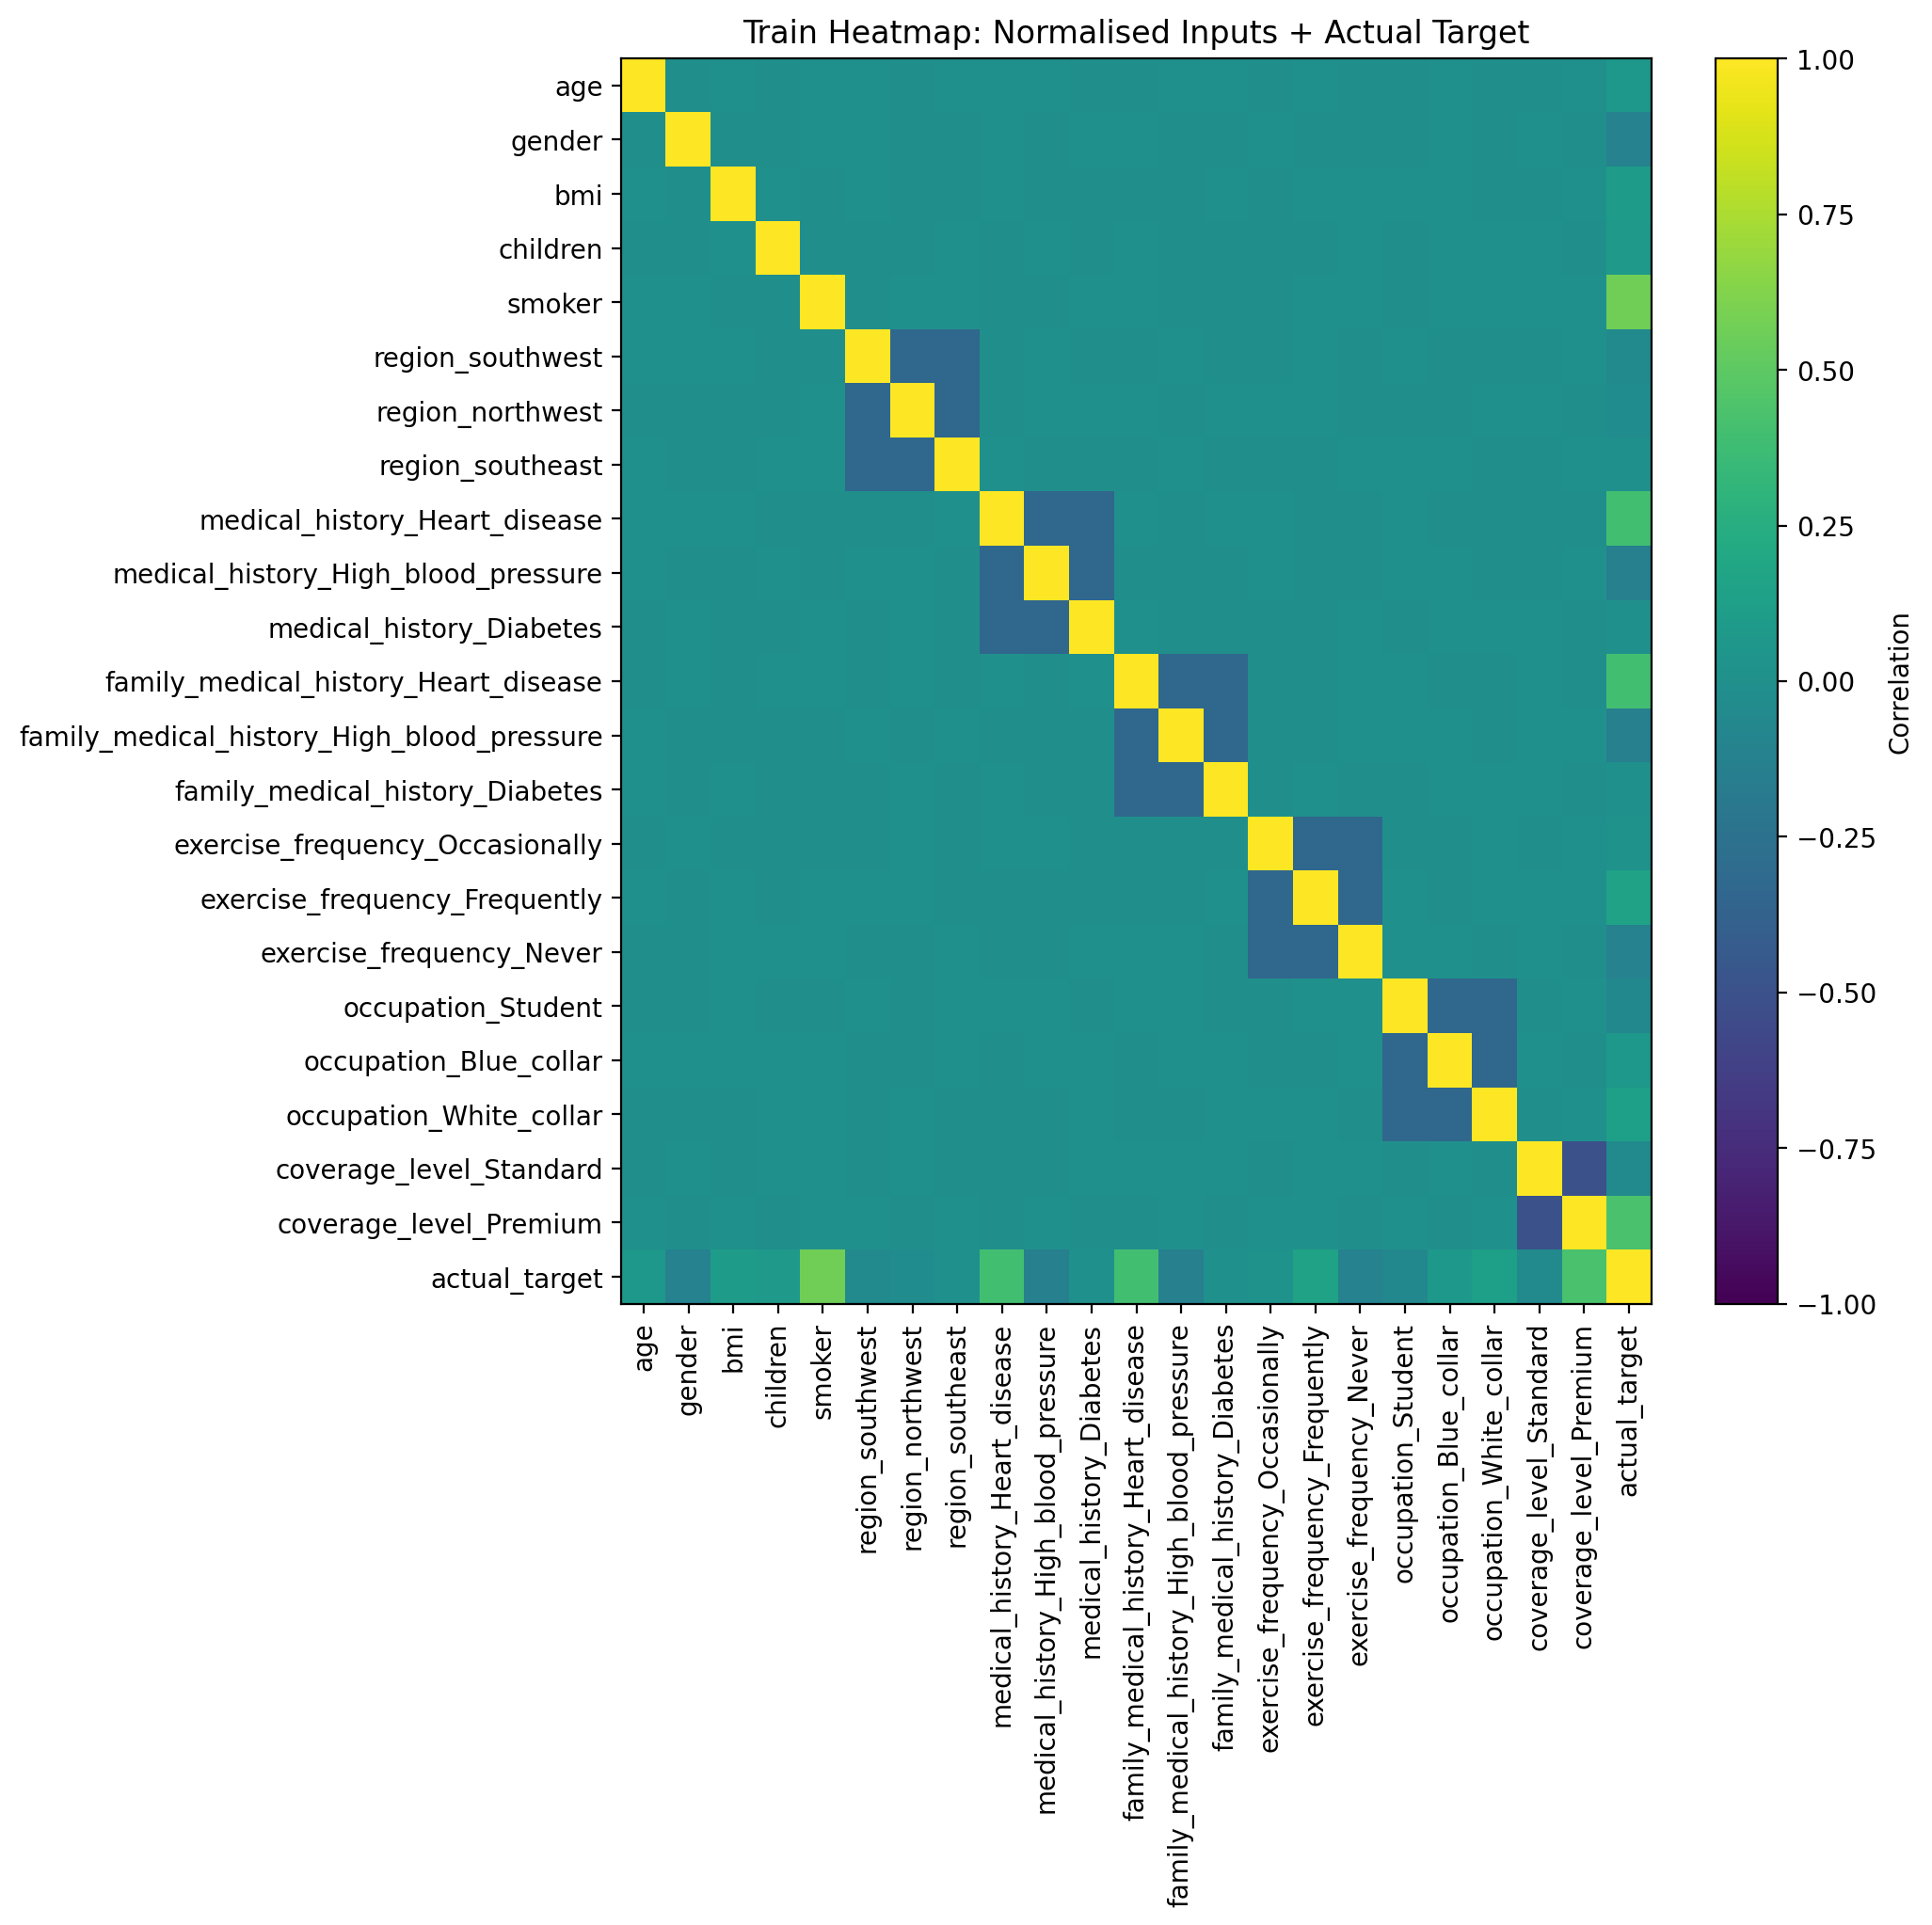
\includegraphics[width=\textwidth]{Thesis/Chapter 3/Figures/fig_sml_heatmap_train_actual.png}
    \caption{Training set, actual charges.}
    \label{fig:heatmap_train_actual_ch3}
\end{subfigure}
\hfill
\begin{subfigure}[b]{0.48\textwidth}
    \centering
    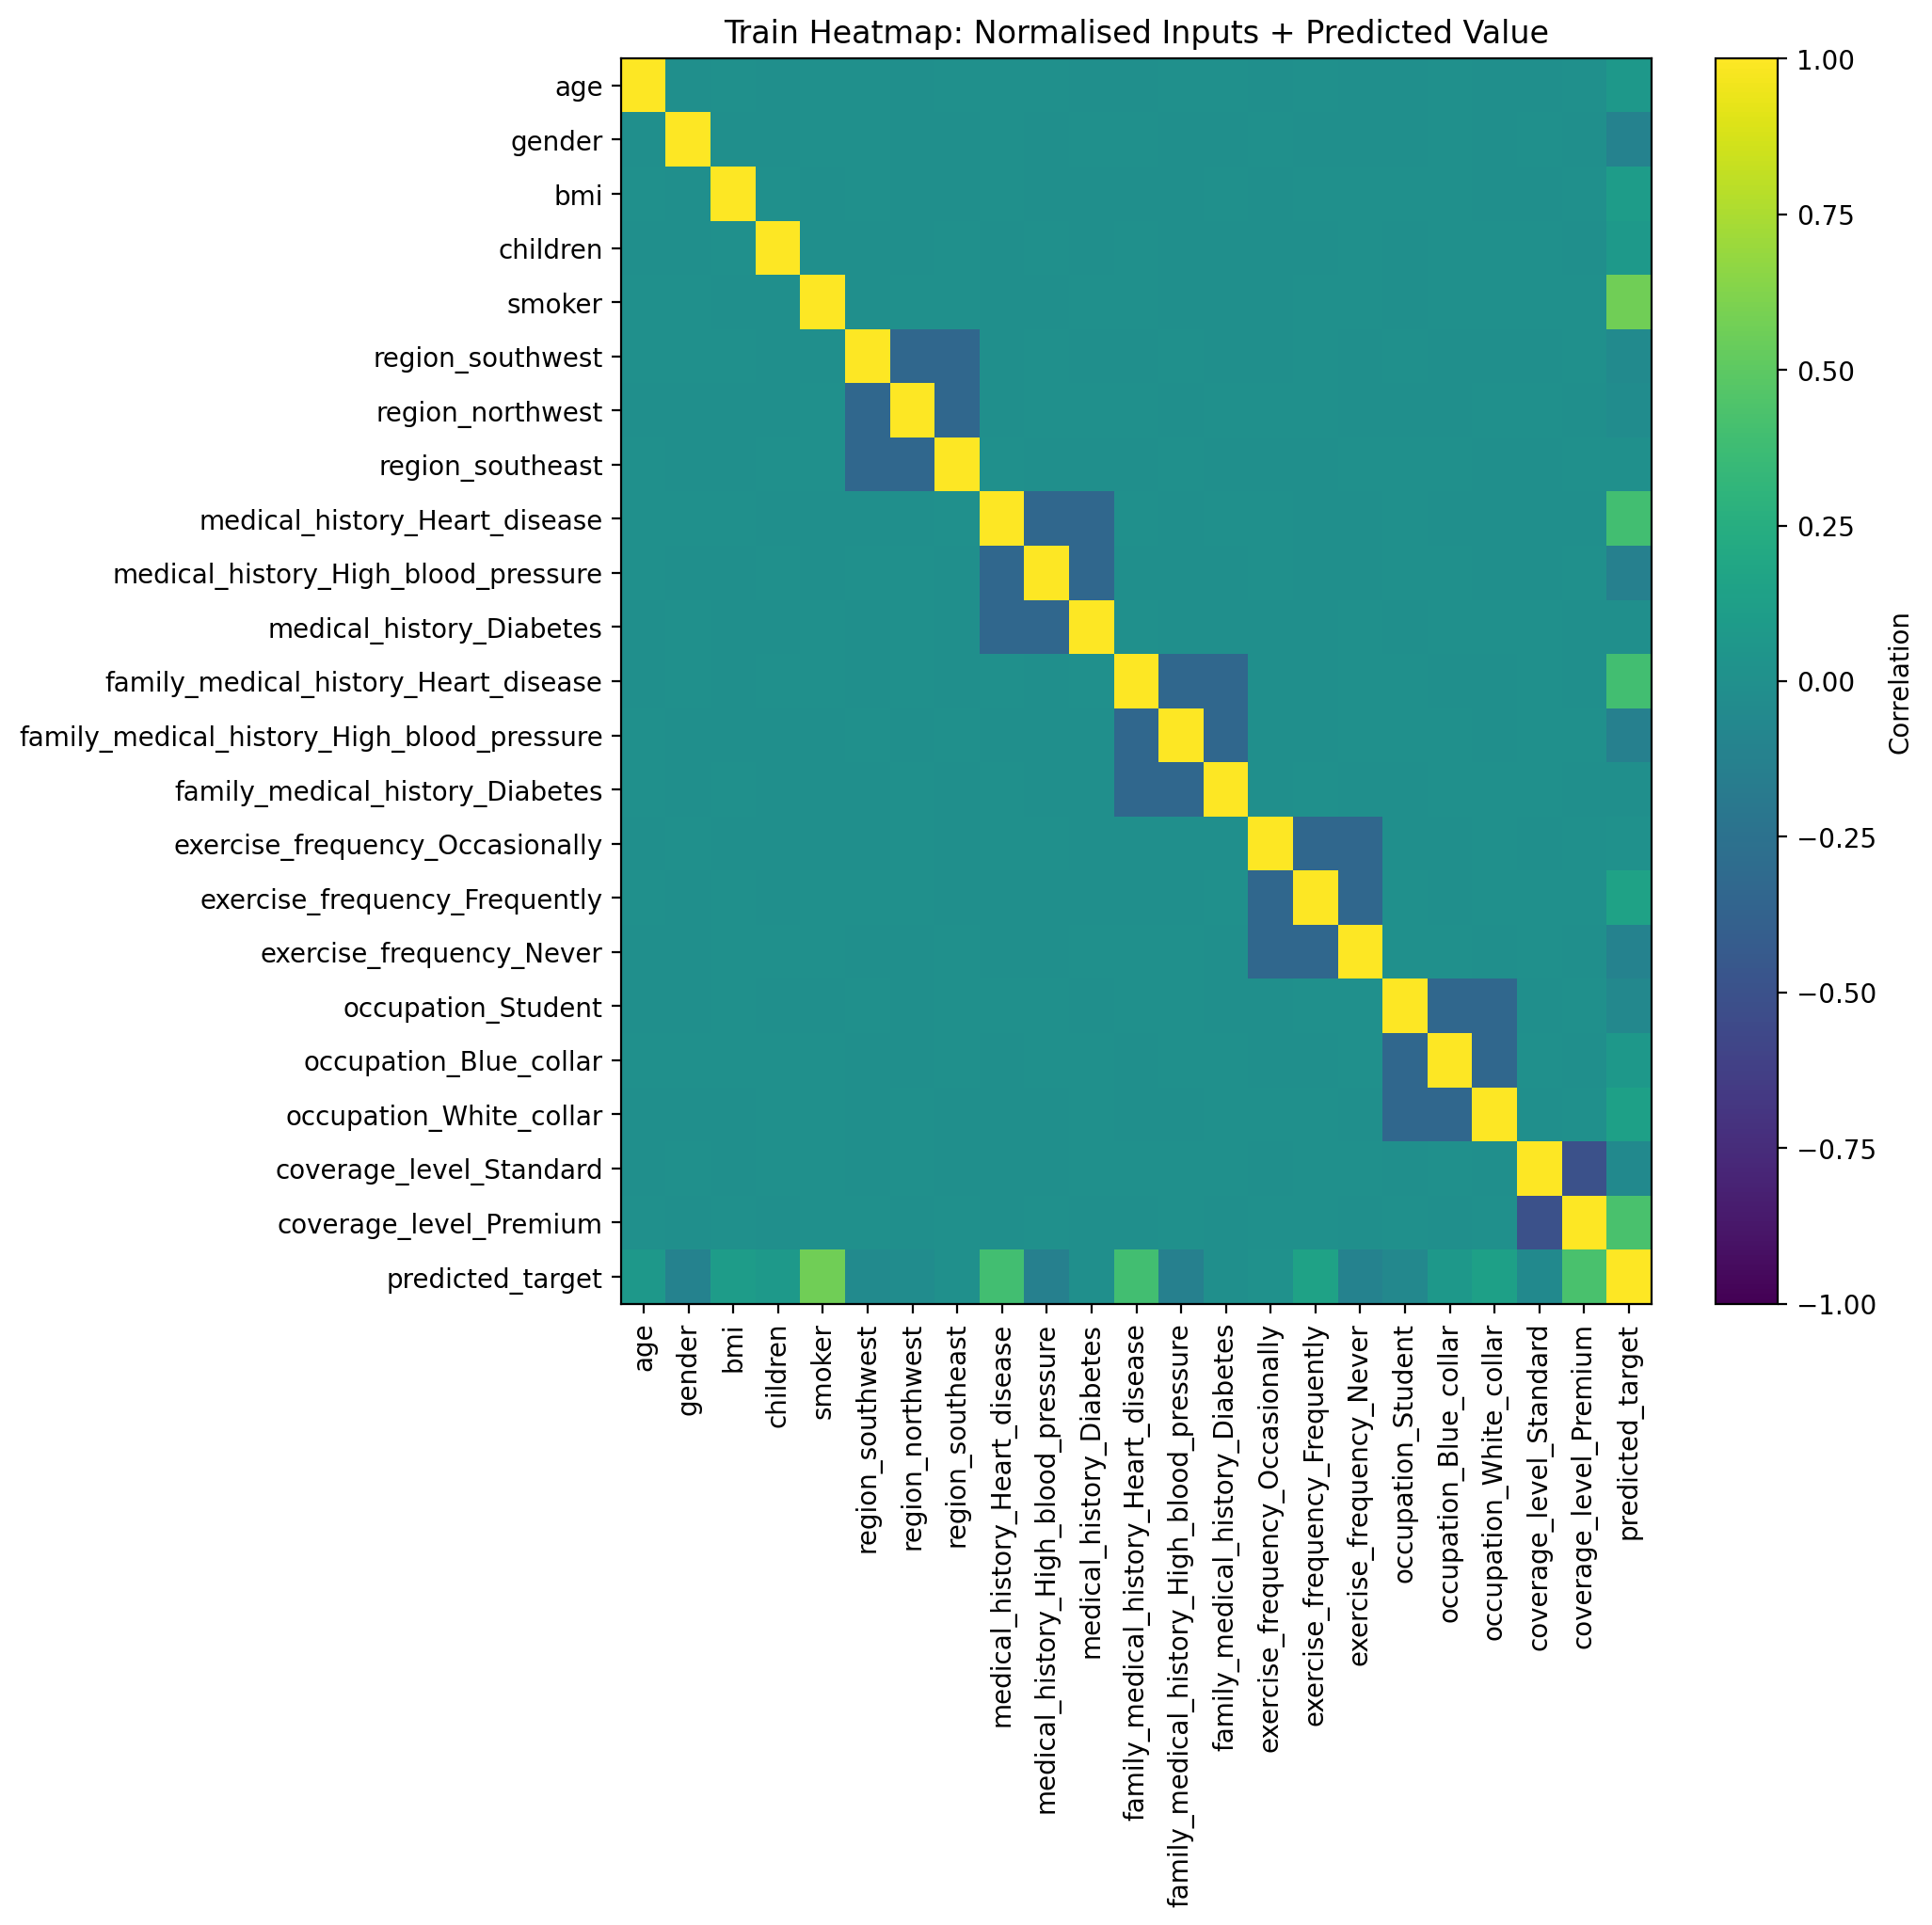
\includegraphics[width=\textwidth]{Thesis/Chapter 3/Figures/fig_sml_heatmap_train_predicted.png}
    \caption{Training set, predicted charges.}
    \label{fig:heatmap_train_predicted_ch3}
\end{subfigure}

\vspace{0.4cm}

\begin{subfigure}[b]{0.48\textwidth}
    \centering
    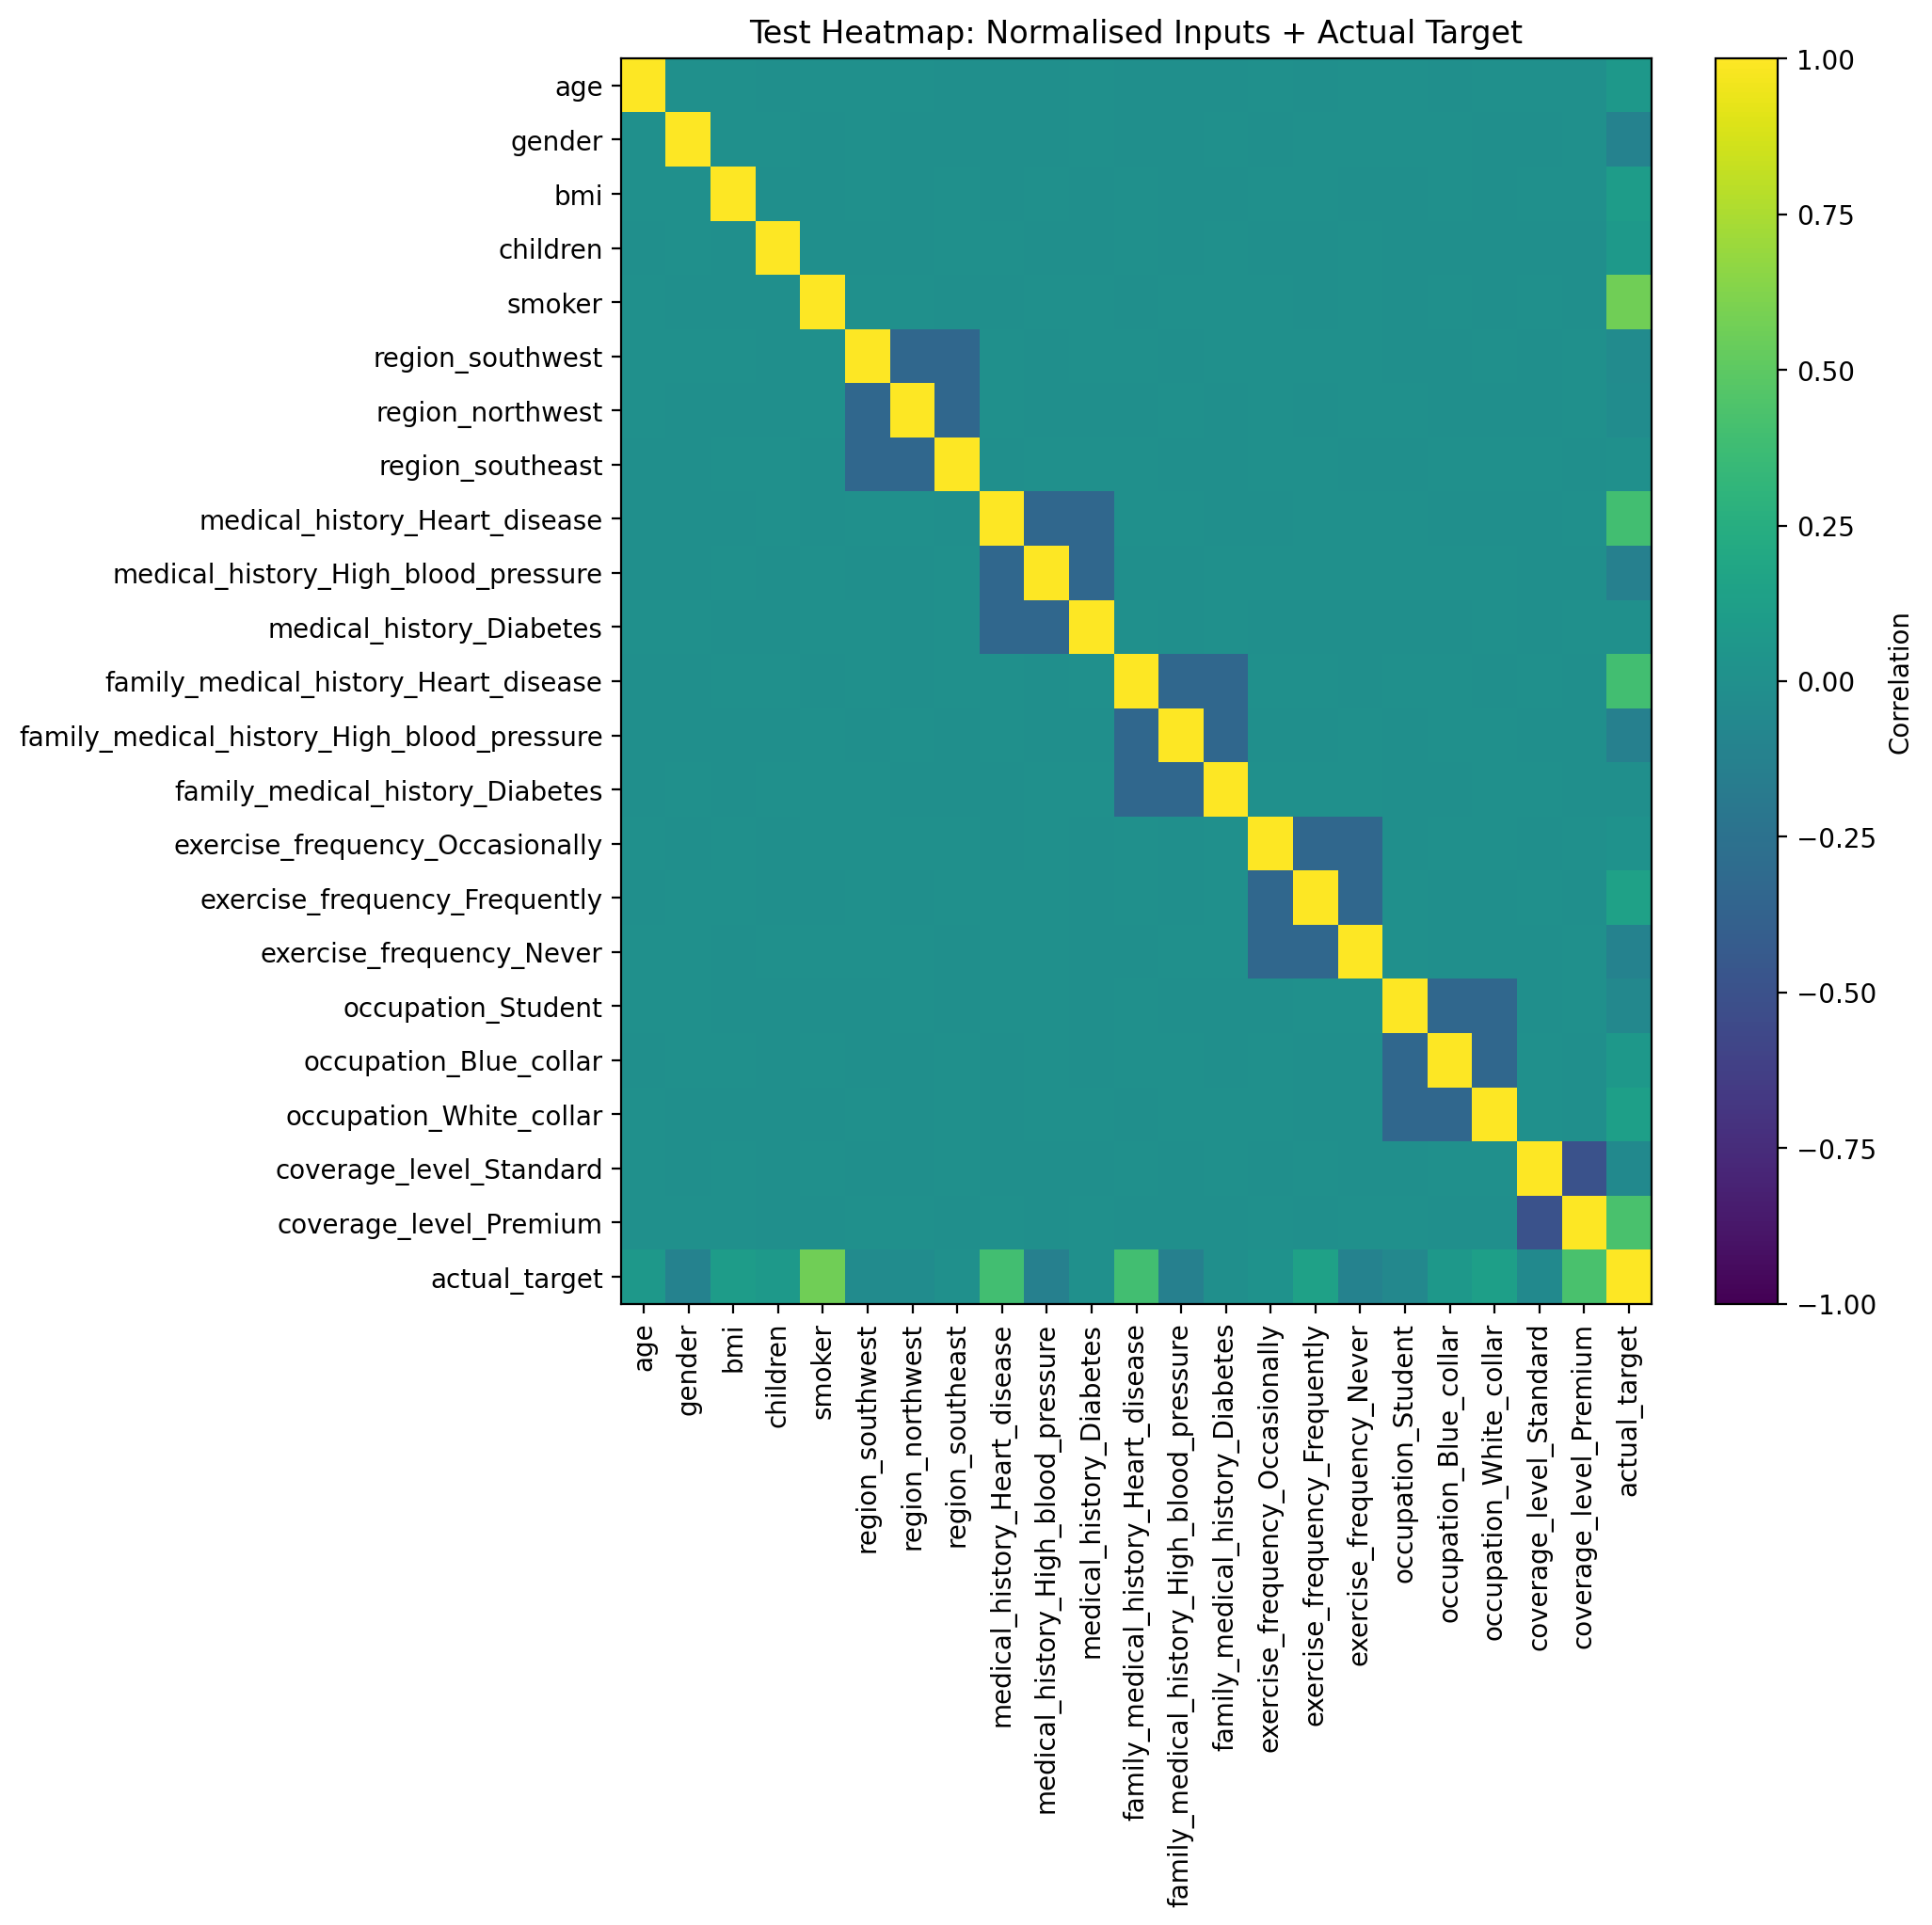
\includegraphics[width=\textwidth]{Thesis/Chapter 3/Figures/fig_sml_heatmap_test_actual.png}
    \caption{Test set, actual charges.}
    \label{fig:heatmap_test_actual_ch3}
\end{subfigure}
\hfill
\begin{subfigure}[b]{0.48\textwidth}
    \centering
    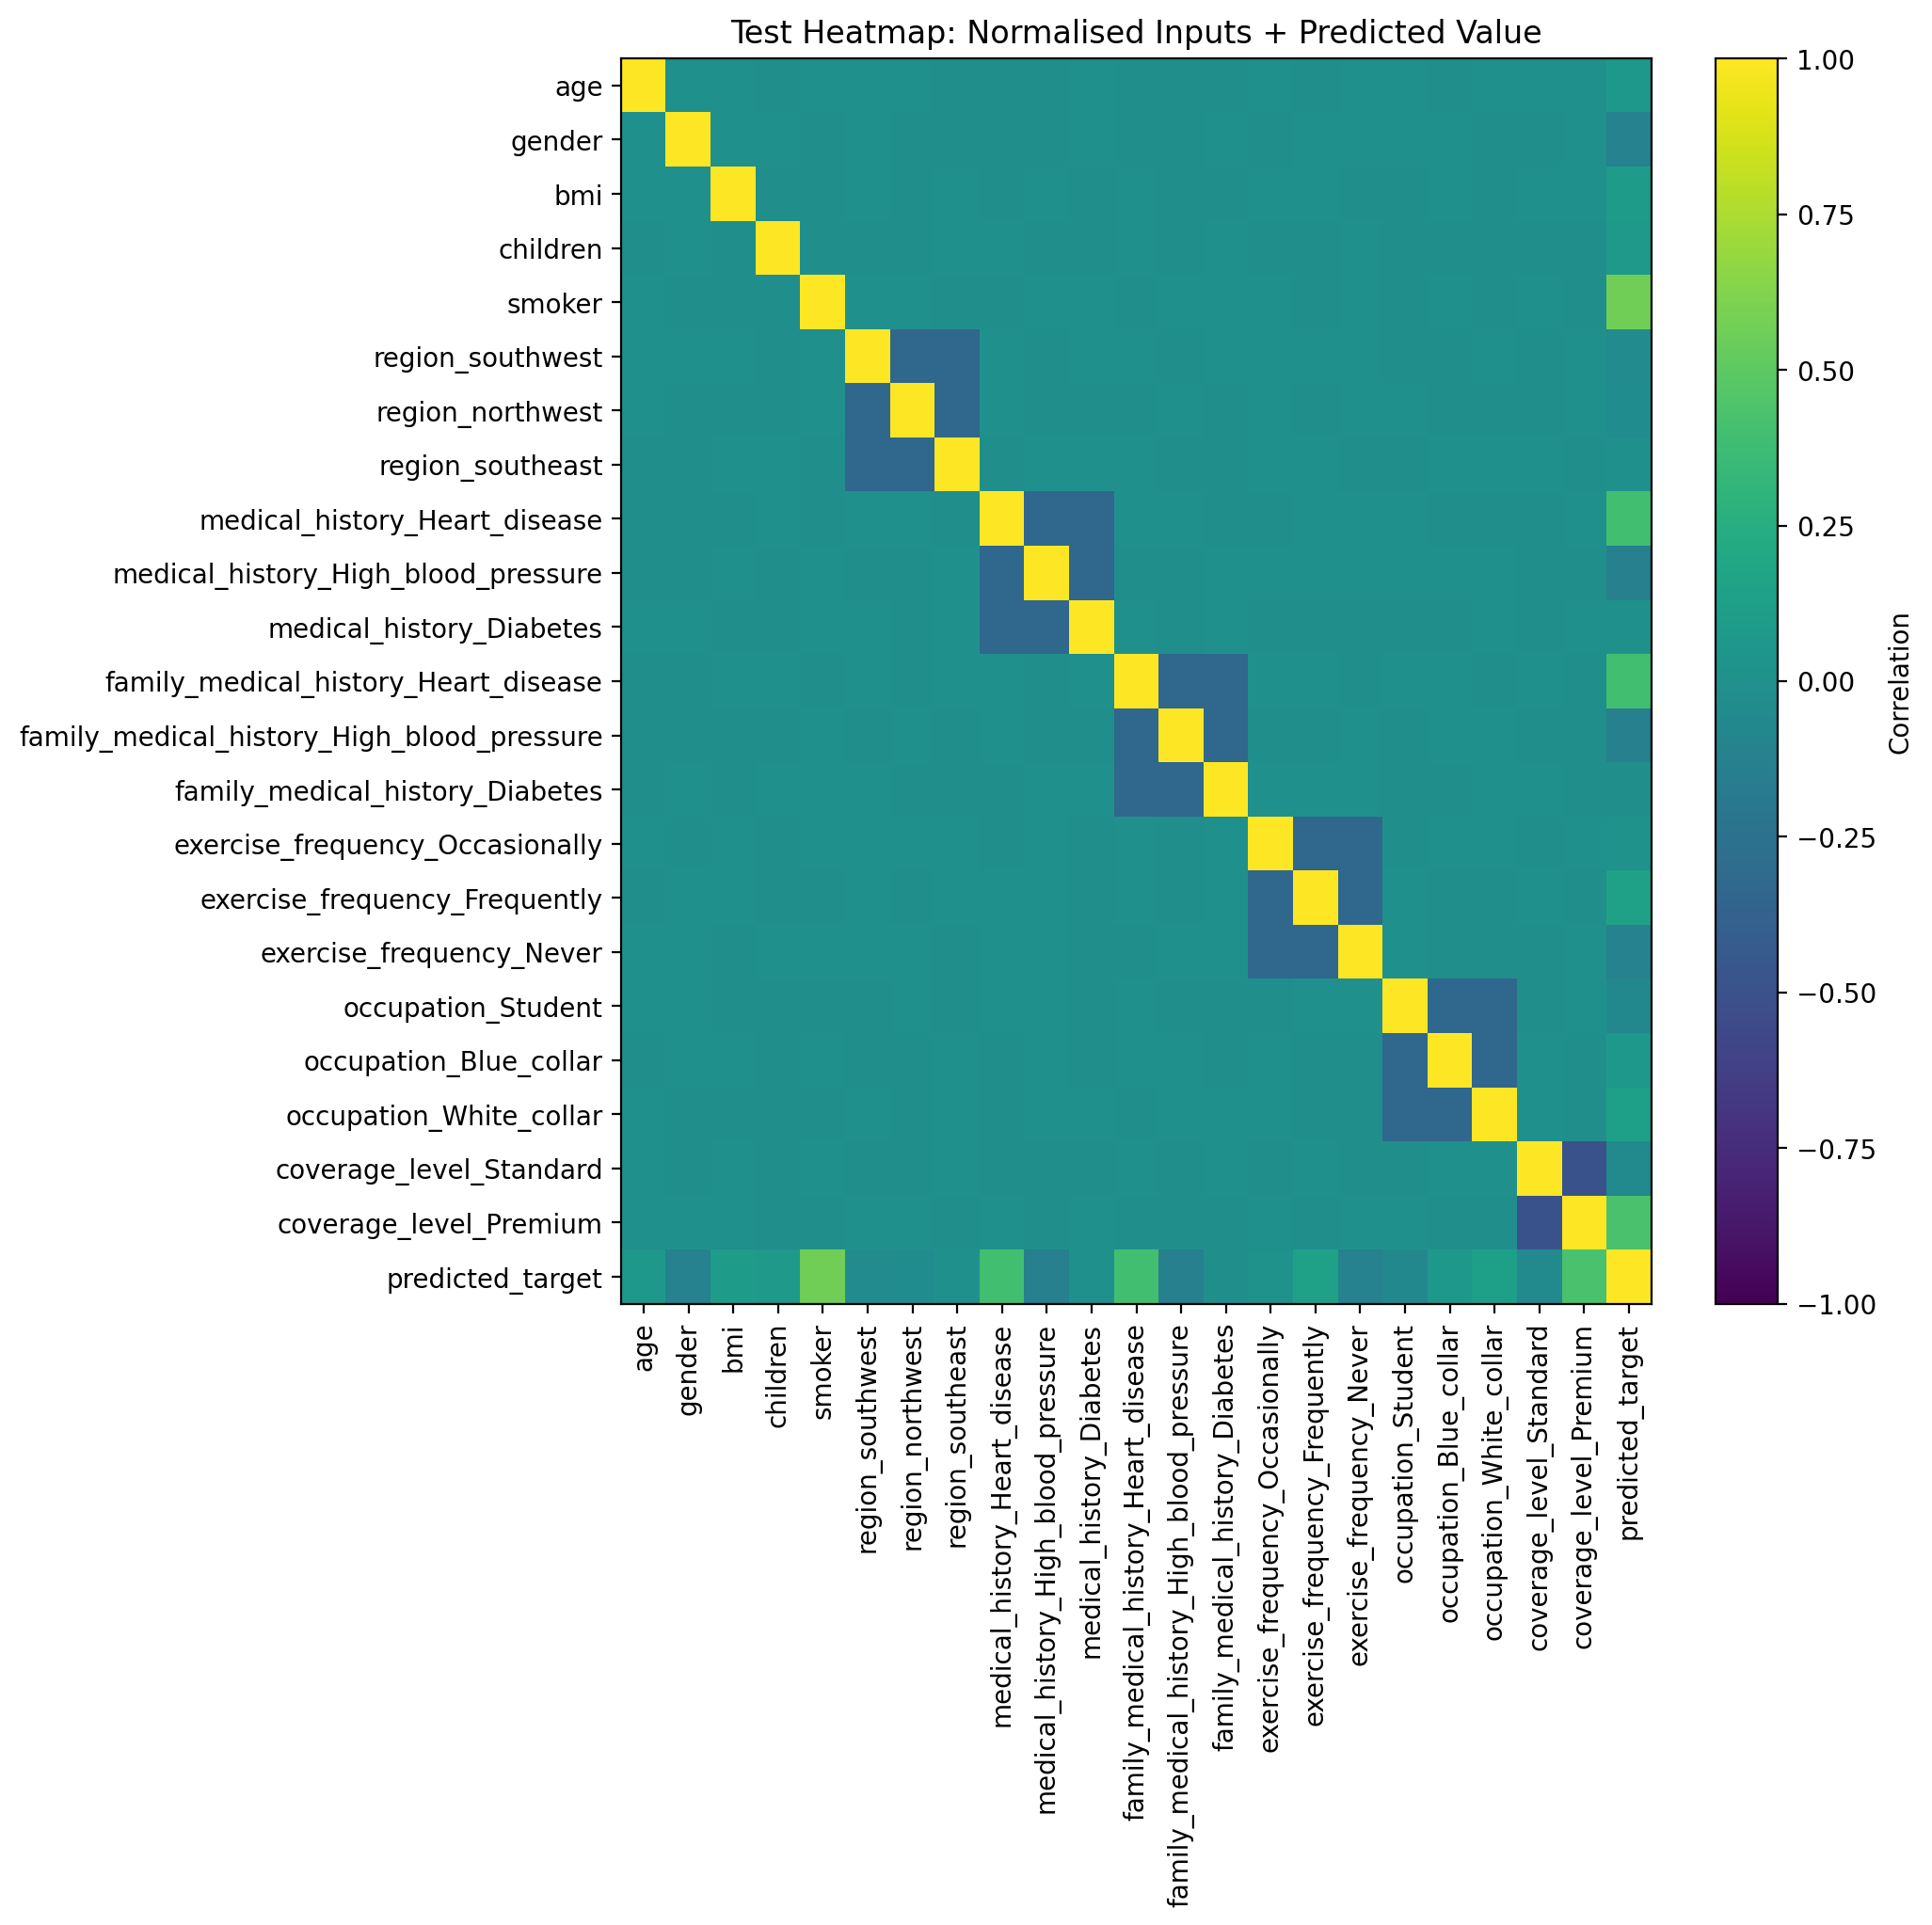
\includegraphics[width=\textwidth]{Thesis/Chapter 3/Figures/fig_sml_heatmap_test_predicted.png}
    \caption{Test set, predicted charges.}
    \label{fig:heatmap_test_predicted_ch3}
\end{subfigure}
\caption{Input-target correlation heatmaps for actual and predicted charges.}
\label{fig:heatmap_diagnostics_ch3}
\end{figure}

\noindent
Figure~\ref{fig:heatmap_diagnostics_ch3} presents the four correlation
heatmaps. The inter-feature correlations are predominantly near zero (teal
shading), with the expected negative correlations visible within dummy
groups belonging to the same raw categorical variable (e.g.\ the
\texttt{medical\_\allowbreak{}history}, \texttt{region}, \texttt{occupation} and
\texttt{coverage\_\allowbreak{}level} dummy blocks). The bottom row of each panel shows
the feature-target correlations. In the training set
(Figure~\ref{fig:heatmap_train_actual_ch3}), \texttt{smoker} shows the
largest positive correlation with actual charges (bright green-yellow),
followed by \texttt{coverage\_level\_\allowbreak{}Premium},
\texttt{medical\_history\_\allowbreak{}Heart\_disease} and \texttt{bmi}. The predicted
version (Figure~\ref{fig:heatmap_train_predicted_ch3}) displays a virtually
identical target row, confirming that the fitted \gls{dnn} has preserved the
linear association structure. The test set
(Figures~\ref{fig:heatmap_test_actual_ch3}
and~\ref{fig:heatmap_test_predicted_ch3}) reproduces the same patterns,
with the target-correlation rows near-identical across both the actual and
predicted versions. These consistency findings complete the diagnostic
verification; the fitted \gls{dnn} is therefore ready to serve as the prediction
surface for the \gls{mc} and Shapley-value analyses that follow.


% =============================================================
\subsection{Parametric MC Simulation Design}
\label{sec:mc_simulation_design}

The \gls{mc} stage generates a synthetic policyholder input space and
the corresponding model-implied distribution of predicted costs.  Each raw
predictor variable is assigned a fitted simulation distribution, synthetic
policyholder profiles are drawn from these distributions, and the fitted
\gls{dnn} computes predicted costs for the generated profiles.  The
simulation is performed at the raw-variable level: categorical variables
are simulated as valid categories first and are only then transformed into
the same encoding used during model training.  Dummy variables are never
simulated independently, since that could produce impossible category
combinations.

\subsubsection{Joint input distribution}

The joint simulation distribution is constructed as a product of fitted
marginal distributions, following the principle of
equation~\eqref{eq:input_law}.  Let
$\mathbf{X}_{\mathrm{raw}} = (X_1, X_2, \ldots, X_q)$ denote the vector of
raw predictor variables, where $q = 11$.  Applying the product-marginal
construction of equation~\eqref{eq:input_law} to the raw variables before
encoding yields
\begin{equation}
    \widehat{F}_{X,\mathrm{raw}}
    =
    \prod_{j=1}^{q}
    \widehat{F}_{X_j}.
    \label{eq:raw_product_mc_distribution_ch3}
\end{equation}
\equationlistentry{Product-marginal \gls{mc} input distribution}
As discussed in Section~\ref{montecarlo_propagation}, the product-marginal
construction is a modelling choice adopted for simulation purposes.  Two
empirical findings from the exploratory analysis support it in this dataset: the weak pairwise
correlations among the numerical predictors reported in
Table~\ref{tab:numeric_correlations}, and the observation that
\texttt{age}, \texttt{bmi}, and \texttt{children} are closely consistent
with independent uniform draws over their observed ranges
(Section~\ref{sec:eda_model_simulation_design}).  The product-marginal
construction is therefore not merely a computational convenience but a
faithful reflection of the benchmark data's apparent generating design.

\subsubsection{Fitted marginal distributions}

The fitted marginal distributions are selected using the empirical summaries
from the exploratory diagnostics.  All distributional parameters, including
the support bounds for the uniform distributions, are estimated from
$\mathcal{D}_{\mathrm{train}}$ only, ensuring that no validation- or
test-set information enters the simulation design.  Bounded numerical
variables are assigned distributions that respect their observed support.
Binary variables are generated from Bernoulli distributions.  Multi-level
categorical variables are generated using the observed training-set
proportions.  Table~\ref{tab:mc_distribution_assumptions_ch3} specifies the
distributional assumptions for each raw variable.

\begin{table}[H]
\centering
\small
\renewcommand{\arraystretch}{1.18}
\begin{tabular}{p{0.20\textwidth}p{0.16\textwidth}p{0.22\textwidth}p{0.20\textwidth}p{0.14\textwidth}}
\toprule
\textbf{Variable} &
\textbf{Type} &
\textbf{Distribution used} &
\textbf{Parameter estimation} &
\textbf{Support} \\
\midrule
\texttt{age} &
Bounded integer &
Discrete uniform &
$\widehat{a}=18,\ \widehat{b}=65$ &
$\{18,\ldots,65\}$ \\
\texttt{bmi} &
Bounded continuous &
Continuous uniform &
$\widehat{a}=18,\ \widehat{b}=50$ &
$[18,50]$ \\
\texttt{children} &
Bounded count &
Discrete uniform &
$\widehat{a}=0,\ \widehat{b}=5$ &
$\{0,\ldots,5\}$ \\
\texttt{gender} &
Binary &
Bernoulli &
$\widehat{p}_{\mathrm{male}} = n_{\mathrm{male}}/n_{\mathrm{train}}$ &
$\{0,1\}$ \\
\texttt{smoker} &
Binary &
Bernoulli &
$\widehat{p}_{\mathrm{yes}} = n_{\mathrm{yes}}/n_{\mathrm{train}}$ &
$\{0,1\}$ \\
\texttt{region} &
Categorical &
Categorical &
$\widehat{p}_{k}=n_k/n_{\mathrm{train}}$ &
Valid regions \\
\texttt{medical\_\allowbreak{}history} &
Categorical &
Categorical &
$\widehat{p}_{k}=n_k/n_{\mathrm{train}}$ &
Valid categories \\
\texttt{family\_medical\_\allowbreak{}history} &
Categorical &
Categorical &
$\widehat{p}_{k}=n_k/n_{\mathrm{train}}$ &
Valid categories \\
\texttt{exercise\_\allowbreak{}frequency} &
Categorical &
Categorical &
$\widehat{p}_{k}=n_k/n_{\mathrm{train}}$ &
Valid categories \\
\texttt{occupation} &
Categorical &
Categorical &
$\widehat{p}_{k}=n_k/n_{\mathrm{train}}$ &
Valid categories \\
\texttt{coverage\_\allowbreak{}level} &
Categorical &
Categorical &
$\widehat{p}_{k}=n_k/n_{\mathrm{train}}$ &
Valid tiers \\
\bottomrule
\end{tabular}
\caption{\gls{mc} input distributions for raw policyholder variables.}
\label{tab:mc_distribution_assumptions_ch3}
\end{table}

The fitted probabilities for categorical variables are estimated from the
training partition only, following the marginal parametric approach in
equation~\eqref{eq:mle_marginal}.  If $C$ is a categorical variable with
levels $c_1,\ldots,c_K$, then
\begin{equation}
    \widehat{p}_{k}
    =
    \frac{1}{n_{\mathrm{train}}}
    \sum_{i \in \mathcal{D}_{\mathrm{train}}}
    \mathbb{I}\{C_i = c_k\},
    \qquad
    k=1,\ldots,K.
    \label{eq:categorical_probability_estimator_ch3}
\end{equation}
\equationlistentry{Categorical probability estimator from training data}
A simulated categorical value is drawn as
$C^{(b)} \sim \operatorname{Categorical}(\widehat{p}_1,\ldots,\widehat{p}_K)$
and subsequently encoded using the reference-category scheme.

\subsubsection{Goodness-of-fit and support checks}

For continuous variables, empirical histograms and density overlays are
inspected, and Kolmogorov-Smirnov (K-S) and Anderson-Darling (A-D)
statistics are recorded.  These two statistics summarise complementary
aspects of marginal fit: the K-S statistic measures the maximum
absolute deviation between the empirical and fitted cumulative distribution
functions, while the A-D statistic places greater weight on the tails,
making it particularly sensitive to distributional departures in the regions
most relevant to the high-cost analysis.  Because the parameters of the
fitted marginals are estimated from the training data, the standard
critical values of these tests are invalid (the Lilliefors problem); the
K-S and A-D statistics are therefore reported as descriptive distance
measures of marginal fit rather than as formal hypothesis tests with
nominal critical values or $p$-values.  Parametric-bootstrap calibration
would be required to obtain valid $p$-values, and is not pursued because
the statistics serve a purely descriptive role here.  For the discrete and
categorical variables (including \texttt{age} and \texttt{children}, to
which continuous-distribution K-S theory does not apply), the comparison
is instead made between the empirical and fitted probability mass
functions, using frequency tables and chi-squared discrepancy summaries
interpreted in the same descriptive spirit.  Because the sample size is
large, even negligibly small distributional differences would be flagged
as significant by formal tests without being practically important for
simulation, which further motivates the descriptive treatment.  Support
restrictions are treated as compulsory: simulated numerical predictors are
confined to their observed ranges and categorical variables take only valid
observed levels.

\subsubsection{Sample size and convergence monitoring}

The base simulation uses $B = 100\,000$ generated policyholder profiles.  A
pilot convergence check is conducted by repeating the simulation for
increasing values of $B \in \{1\,000,\ 2\,500,\ 5\,000,\ 10\,000,\
25\,000,\ 50\,000,\ 100\,000\}$.  For each $B$, the running mean, standard deviation, and
selected quantiles of the simulated predicted costs are recorded.  The Monte
Carlo standard error is estimated using equation~\eqref{eq:mcse}, with
$s_B$ denoting the simulated standard deviation.  This mean-based
\gls{mcse} formula does not apply to quantiles: for a quantile level
$u \in (0,1)$, the Monte Carlo uncertainty is instead governed by the
asymptotic variance
$u(1-u)/\bigl(B\,f\bigl(F^{-1}(u)\bigr)^{2}\bigr)$, where $f$ denotes the
density of the predicted-cost distribution at the quantile of interest;
percentile stability is therefore assessed descriptively across the
increasing pilot sizes.  The selected simulation
size is retained when running summaries are stable relative to the scale of
the response variable.

\begin{table}[H]
\centering
\small
\renewcommand{\arraystretch}{1.15}
\begin{tabular}{p{0.25\textwidth}p{0.60\textwidth}}
\toprule
\textbf{Quantity} & \textbf{Purpose} \\
\midrule
Running mean & Checks stability of the average simulated predicted cost \\
Running standard deviation & Checks stability of simulated output spread \\
Median & Checks central distributional stability \\
90th percentile & Checks upper-tail stability \\
95th percentile & Candidate high-cost threshold \\
99th percentile & Extreme upper-tail stability check \\
\gls{mcse} & Quantifies simulation precision for selected summaries \\
\bottomrule
\end{tabular}
\caption{\gls{mc} convergence quantities recorded during the pilot run.}
\label{tab:mc_convergence_quantities_ch3}
\end{table}

\subsubsection{Base DNN MC scoring}

For each simulated raw profile, the preprocessing map $T(\cdot)$ produces
the model-ready input vector $\mathbf{z}^{(b)}$.  The fitted \gls{dnn} then
calculates the base \gls{mc} prediction, following the formulation in
equation~\eqref{eq:mc_predictions_framework}:
\begin{equation}
    \widehat{Y}^{(b)}
    =
    \widehat{m}
    \left(
        \mathbf{z}^{(b)}
    \right),
    \qquad
    b=1,\ldots,B.
    \label{eq:base_mc_prediction_ch3}
\end{equation}
\equationlistentry{Base \gls{mc} \gls{dnn} prediction}
The resulting collection
$\{\widehat{Y}^{(1)},\ldots,\widehat{Y}^{(B)}\}$
forms the base model-implied predicted-cost distribution introduced in
equation~\eqref{eq:mc_predictions_framework}.  The generated input profiles are also summarised
before interpreting the predicted-cost outputs, to confirm what type of
simulated input space produced the \gls{dnn} predictions.

\begin{table}[H]
\centering
\small
\renewcommand{\arraystretch}{1.15}
\begin{tabular}{p{0.92\textwidth}}
\toprule
\textbf{Algorithm 3.1: Base parametric \gls{mc} simulation} \\
\midrule
\textbf{Input:} fitted raw-variable distributions
$\{\widehat{F}_{X_j}\}_{j=1}^{q}$, fitted model
$\widehat{m}(\cdot)$, preprocessing map $T(\cdot)$, number of
replications $B$, random seed $s$. \\[3pt]

\textbf{Output:} simulated raw profiles
$\{\mathbf{X}_{\mathrm{raw}}^{(b)}\}_{b=1}^{B}$, model-ready profiles
$\{\mathbf{z}^{(b)}\}_{b=1}^{B}$, and base predicted costs
$\{\widehat{Y}^{(b)}\}_{b=1}^{B}$. \\[3pt]

1. Set the random seed to $s$. \\
2. For $b=1,\ldots,B$, simulate each raw variable from its fitted marginal distribution. \\
3. For categorical variables, simulate a valid category before applying reference-category encoding. \\
4. Apply the training-set preprocessing map $T(\cdot)$ to obtain $\mathbf{z}^{(b)}$. \\
5. Calculate $\widehat{Y}^{(b)} = \widehat{m}(\mathbf{z}^{(b)})$. \\
6. Transform predictions back to the original monetary scale if the network output is on the standardised scale. \\
7. Store the simulated inputs, encoded inputs and predicted costs. \\
\bottomrule
\end{tabular}
\caption{Base \gls{mc} simulation algorithm.}
\label{tab:base_mc_algorithm_ch3}
\end{table}

% =============================================================
\subsection{Validation of the MC Input Distribution}
\label{sec:mc_input_validation}

The product-marginal simulation law in
equation~\eqref{eq:raw_product_mc_distribution_ch3} constructs the joint
input distribution as a product of independent fitted marginals. Even if
every marginal distribution matches the training data closely, the joint
distribution of the simulated profiles is structurally different from the
joint distribution of the training data because all cross-variable
dependencies are set to zero by construction. This section diagnoses the
magnitude of that joint-distribution difference and then assesses whether it
affects the Shapley-value attributions derived from the simulated profiles.

\subsubsection{Joint distribution diagnostics}

The first diagnostic examines the difference between correlation
matrices.  Because Pearson correlation is undefined for unordered nominal
variables such as \texttt{region}, \texttt{occupation} and
\texttt{medical\_\allowbreak{}history}, this comparison is carried out on
the model-ready encoded representation, in which the numerical variables
enter directly and each categorical variable enters through its binary
dummy indicators.  The Pearson correlation matrix of the encoded columns
is computed separately on the training partition and on the parametric
\gls{mc} sample. The element-wise difference
\begin{equation}
    \Delta_{jk}
    =
    r_{jk}^{(\mathrm{train})}
    -
    r_{jk}^{(\mathrm{MC})},
    \qquad
    j,k = 1,\ldots,p,
    \label{eq:correlation_difference_ch3}
\end{equation}
\equationlistentry{Correlation matrix difference (training minus \gls{mc})}
quantifies how the pairwise linear association structure of the simulated
profiles deviates from that of the training data. Because the parametric
\gls{mc} sample draws each raw variable independently, the correlations
between encoded columns derived from different raw variables are
approximately zero by construction (the mechanical negative correlations
within a dummy group arise in both datasets), so
$\Delta_{jk} \approx r_{jk}^{(\mathrm{train})}$ for column pairs from
different raw variables. The resulting difference heatmap therefore
reveals which variable pairs carry the strongest dependencies in the
training data that are absent from the simulation.  Linear correlation on
binary indicators is a limited measure of association for nominal
attributes, so this diagnostic is complemented by the Cram\'{e}r's $V$
comparison below, which measures categorical association directly.

\begin{figure}[H]
\centering
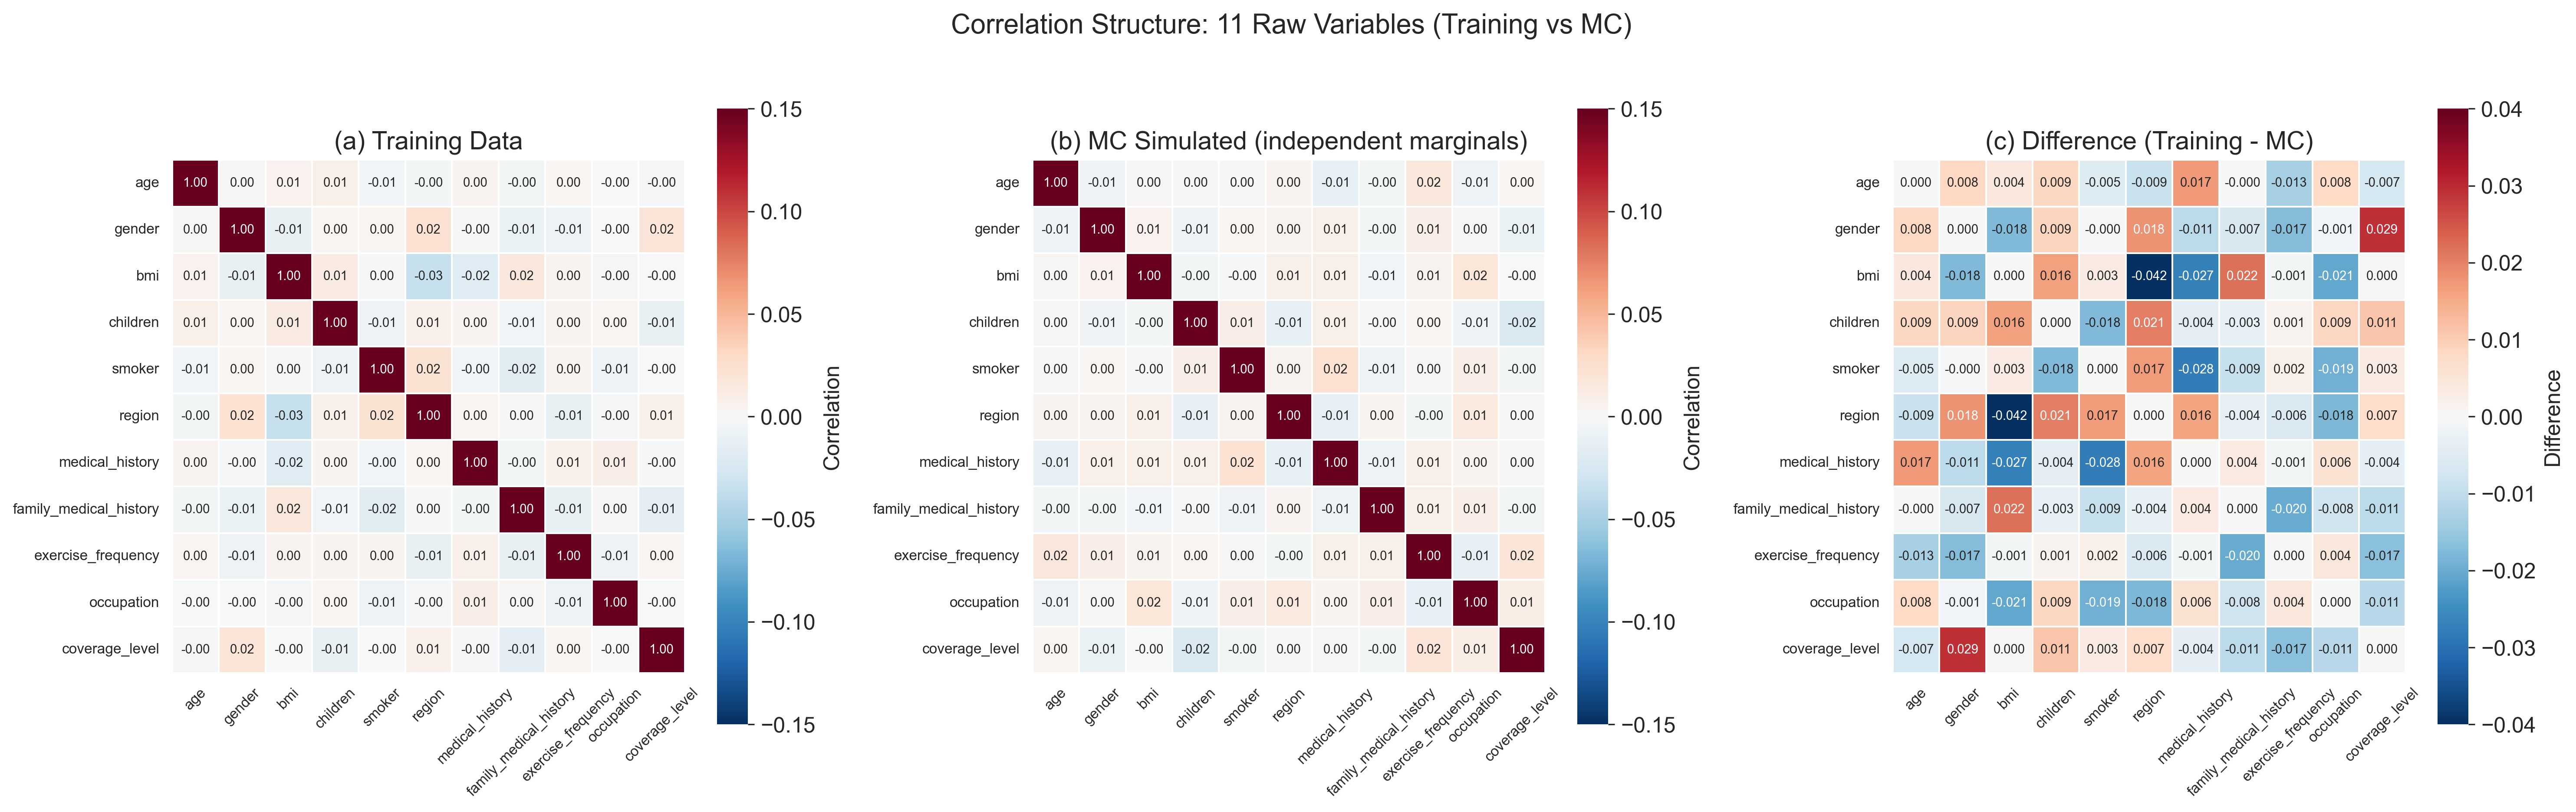
\includegraphics[width=0.90\textwidth]{Thesis/Chapter 3/Figures/fig_mc_joint_correlation_comparison.png}
\caption{Correlation structure comparison: training data versus parametric \gls{mc} sample.}
\label{fig:correlation_difference_heatmap_ch3}
\end{figure}

The second diagnostic addresses the categorical predictors.  For
multi-level categorical predictors the strength of pairwise association is
measured using Cram\'{e}r's $V$ statistic \citep{cramer1946mathematical}.
For each pair of categorical variables, $V$ is computed on the training
partition and on the parametric \gls{mc} sample. All pairwise values of
$V$ are compared to confirm that cross-variable associations are below a
weak-association threshold in both datasets and that the parametric \gls{mc}
sample, which has exactly zero association by construction, does not
materially differ from the training data.

\begin{figure}[H]
\centering
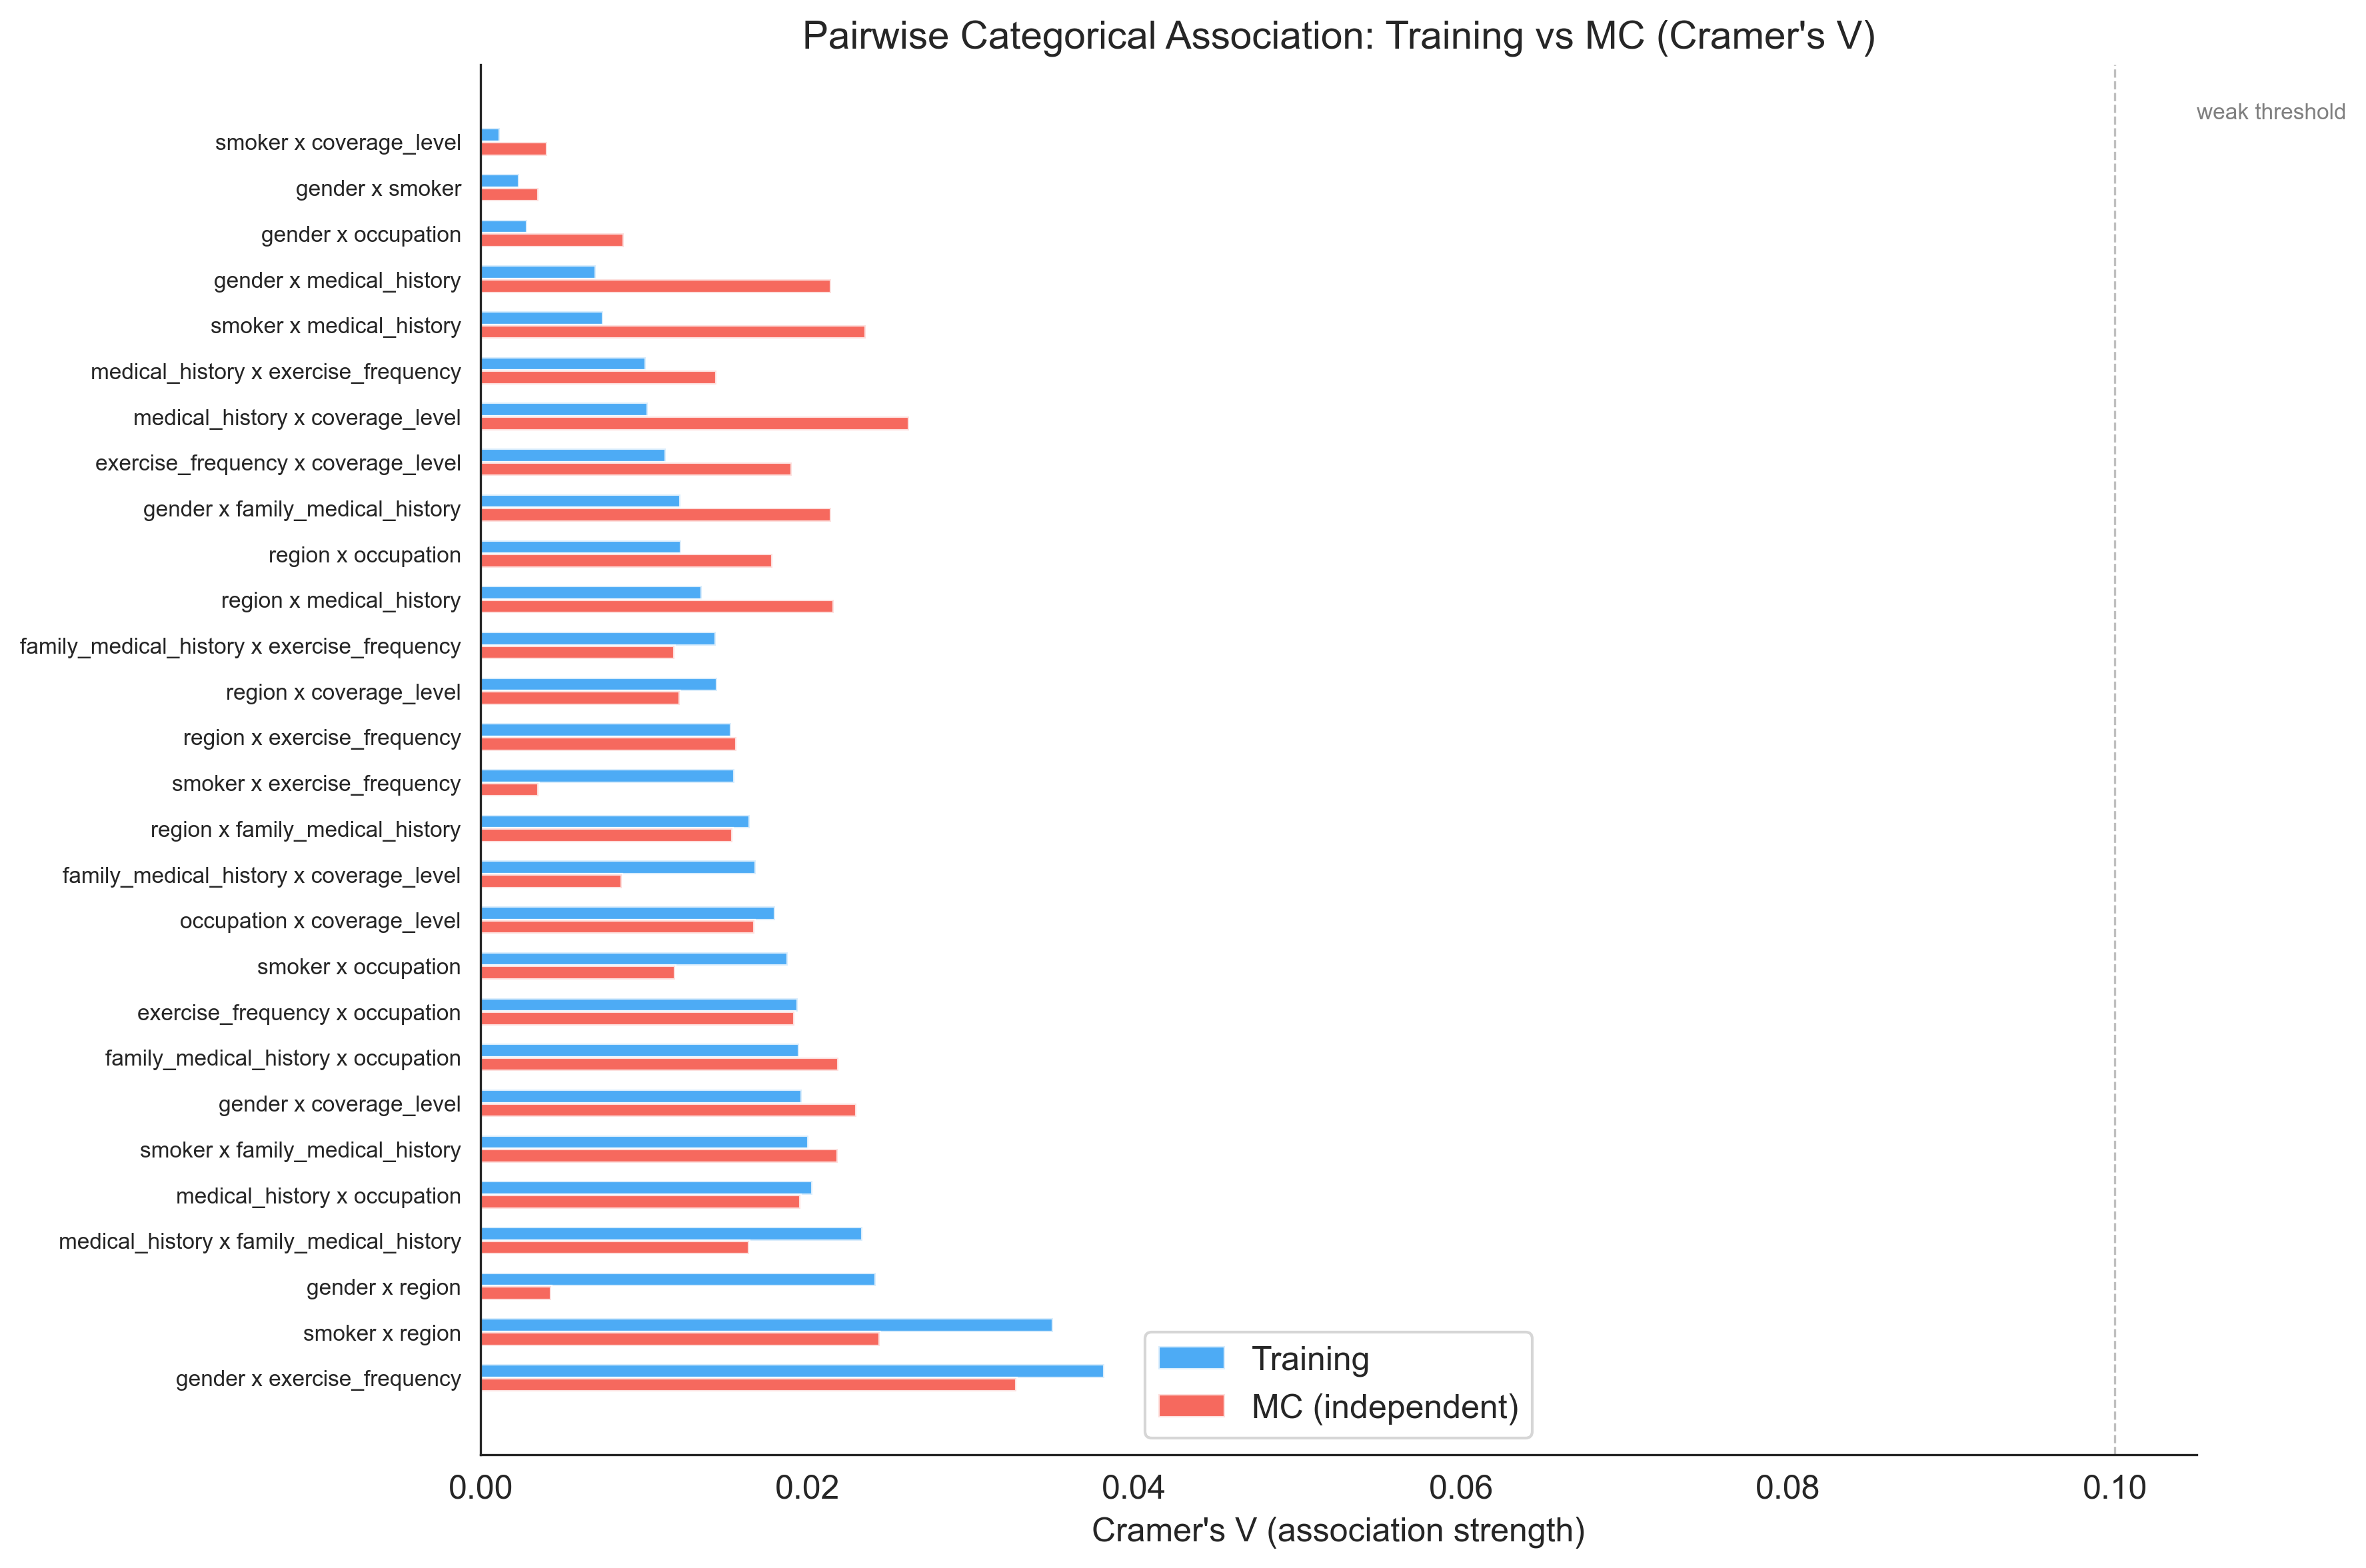
\includegraphics[width=0.90\textwidth]{Thesis/Chapter 3/Figures/fig_mc_joint_cramers_v.png}
\caption{Cram\'{e}r's $V$ comparison: training versus parametric \gls{mc} sample.}
\label{fig:cramers_v_comparison_ch3}
\end{figure}

The third diagnostic is a \gls{pca} overlay of the joint input space.
A principal component projection provides a visual comparison of the joint
input structure. The first two principal components are computed from the
standardised training inputs (using the eigenvectors from
Section~\ref{sec:pca_structural_diagnostics}), and both the training set
and the parametric \gls{mc} sample are projected onto these components. The two
point clouds are overlaid with distinct colours. If the independence
assumption substantially alters the joint structure, the \gls{mc} cloud will
appear more spread out or exhibit less internal clustering than the training
cloud. As reported in Section~\ref{sec:pca_structural_diagnostics}
(Figure~\ref{fig:pca_loadings_ch3}), the first two principal components are
dominated by the \texttt{coverage\_\allowbreak{}level} variable yet together
account for only about $13\%$ of total variance, so no single direction
dominates the 22-dimensional input space.

\begin{figure}[H]
\centering
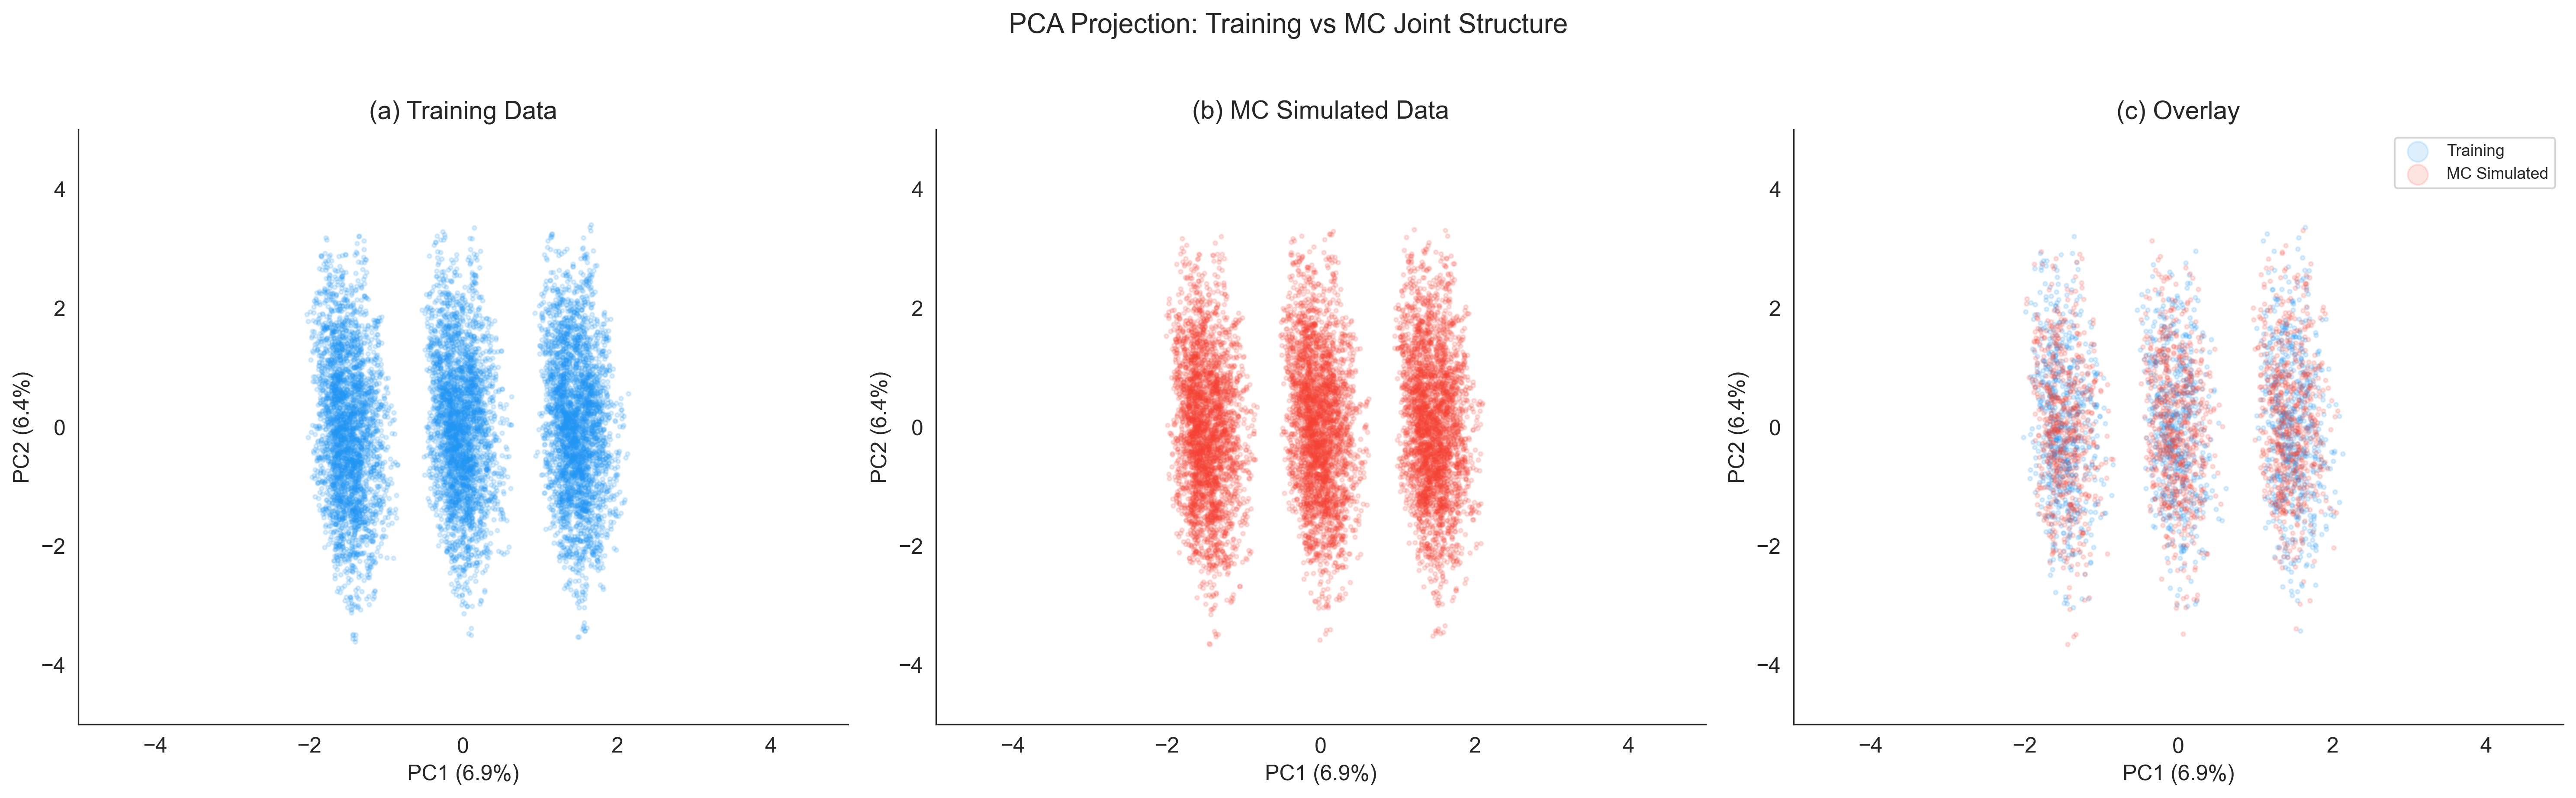
\includegraphics[width=0.95\textwidth]{Thesis/Chapter 3/Figures/fig_mc_joint_pca_comparison.png}
\caption{\Gls{pca} projection of joint input structure: training, \gls{mc} sample and overlay.}
\label{fig:pca_joint_overlay_ch3}
\end{figure}

\noindent
The \gls{mc} sample populates the same region of principal component
space as the training data. The vertical banding visible in both panels
reflects the discrete structure introduced by the categorical predictors.
The overlay in panel~(c) confirms that the two point clouds are broadly
co-located, with the \gls{mc} cloud exhibiting a marginally wider spread
consistent with the removal of the weak dependencies identified in the
correlation analysis.

\subsubsection{Bootstrap MC resampling}
\label{sec:bootstrap_mc_resampling}

To separate the effect of the independence assumption from the effect of
marginal distribution choice, a second \gls{mc} sample of size $B$ is
drawn via bootstrap resampling with replacement from the training set:
\begin{equation}
    \mathbf{X}_{\mathrm{raw}}^{(b,\mathrm{boot})}
    \sim
    \widehat{F}_{X,\mathrm{emp}},
    \qquad
    b = 1, \ldots, B,
    \label{eq:bootstrap_mc_ch3}
\end{equation}
\equationlistentry{Bootstrap \gls{mc} resampling from empirical distribution}
where $\widehat{F}_{X,\mathrm{emp}}$ is the empirical distribution of the
training data. This sample preserves the empirical joint distribution
exactly, including all cross-variable dependencies, while the parametric \gls{mc}
sample uses independent marginals. The bootstrap profiles are preprocessed
and scored through the fitted \gls{dnn} in the same manner as the
parametric profiles. Shapley values are then computed for both sets of
profiles using identical explainer settings, allowing a direct comparison of
the attribution results under the two input regimes.

\begin{table}[H]
\centering
\small
\renewcommand{\arraystretch}{1.15}
\begin{tabular}{p{0.24\textwidth}p{0.33\textwidth}p{0.33\textwidth}}
\toprule
\textbf{Property} & \textbf{Parametric \gls{mc}} & \textbf{Bootstrap \gls{mc}} \\
\midrule
Marginals &
Fitted parametric (uniform, Bernoulli, categorical) &
Empirical (training-set resampled) \\

Joint structure &
Independent (product of marginals) &
Empirical (preserves all dependencies) \\

Sample size &
$B = 100{,}000$ &
$B = 100{,}000$ \\

Purpose &
Primary simulation for cost distribution and Shapley analysis &
Validation check for Shapley invariance to input dependence \\
\bottomrule
\end{tabular}
\caption{Comparison of the two \gls{mc} input regimes.}
\label{tab:mc_input_regimes_ch3}
\end{table}

\subsubsection{Shapley invariance assessment}

The mean absolute Shapley values $I_g$ are aggregated to the raw-variable
level ($q = 11$ variables) and compared between the parametric \gls{mc} and
bootstrap \gls{mc} profiles. If the Shapley attributions are driven by the fitted
\gls{dnn}'s internal importance structure rather than by the particular
dependence pattern in the input profiles, the two sets of attributions
should be nearly identical.

The comparison is summarised by the Spearman rank correlation between the
two feature-importance vectors:
\begin{equation}
    \rho_{\mathrm{S}}
    =
    \operatorname{Spearman}
    \!\left(
        \{I_g^{(\mathrm{param})}\}_{g=1}^{q},\;
        \{I_g^{(\mathrm{boot})}\}_{g=1}^{q}
    \right).
    \label{eq:spearman_shapley_invariance_ch3}
\end{equation}
\equationlistentry{Spearman rank correlation for Shapley invariance}
A rank correlation close to one indicates that the feature-importance
ordering is preserved regardless of whether the input profiles carry
training-data dependencies or assume full independence.

\begin{figure}[H]
\centering
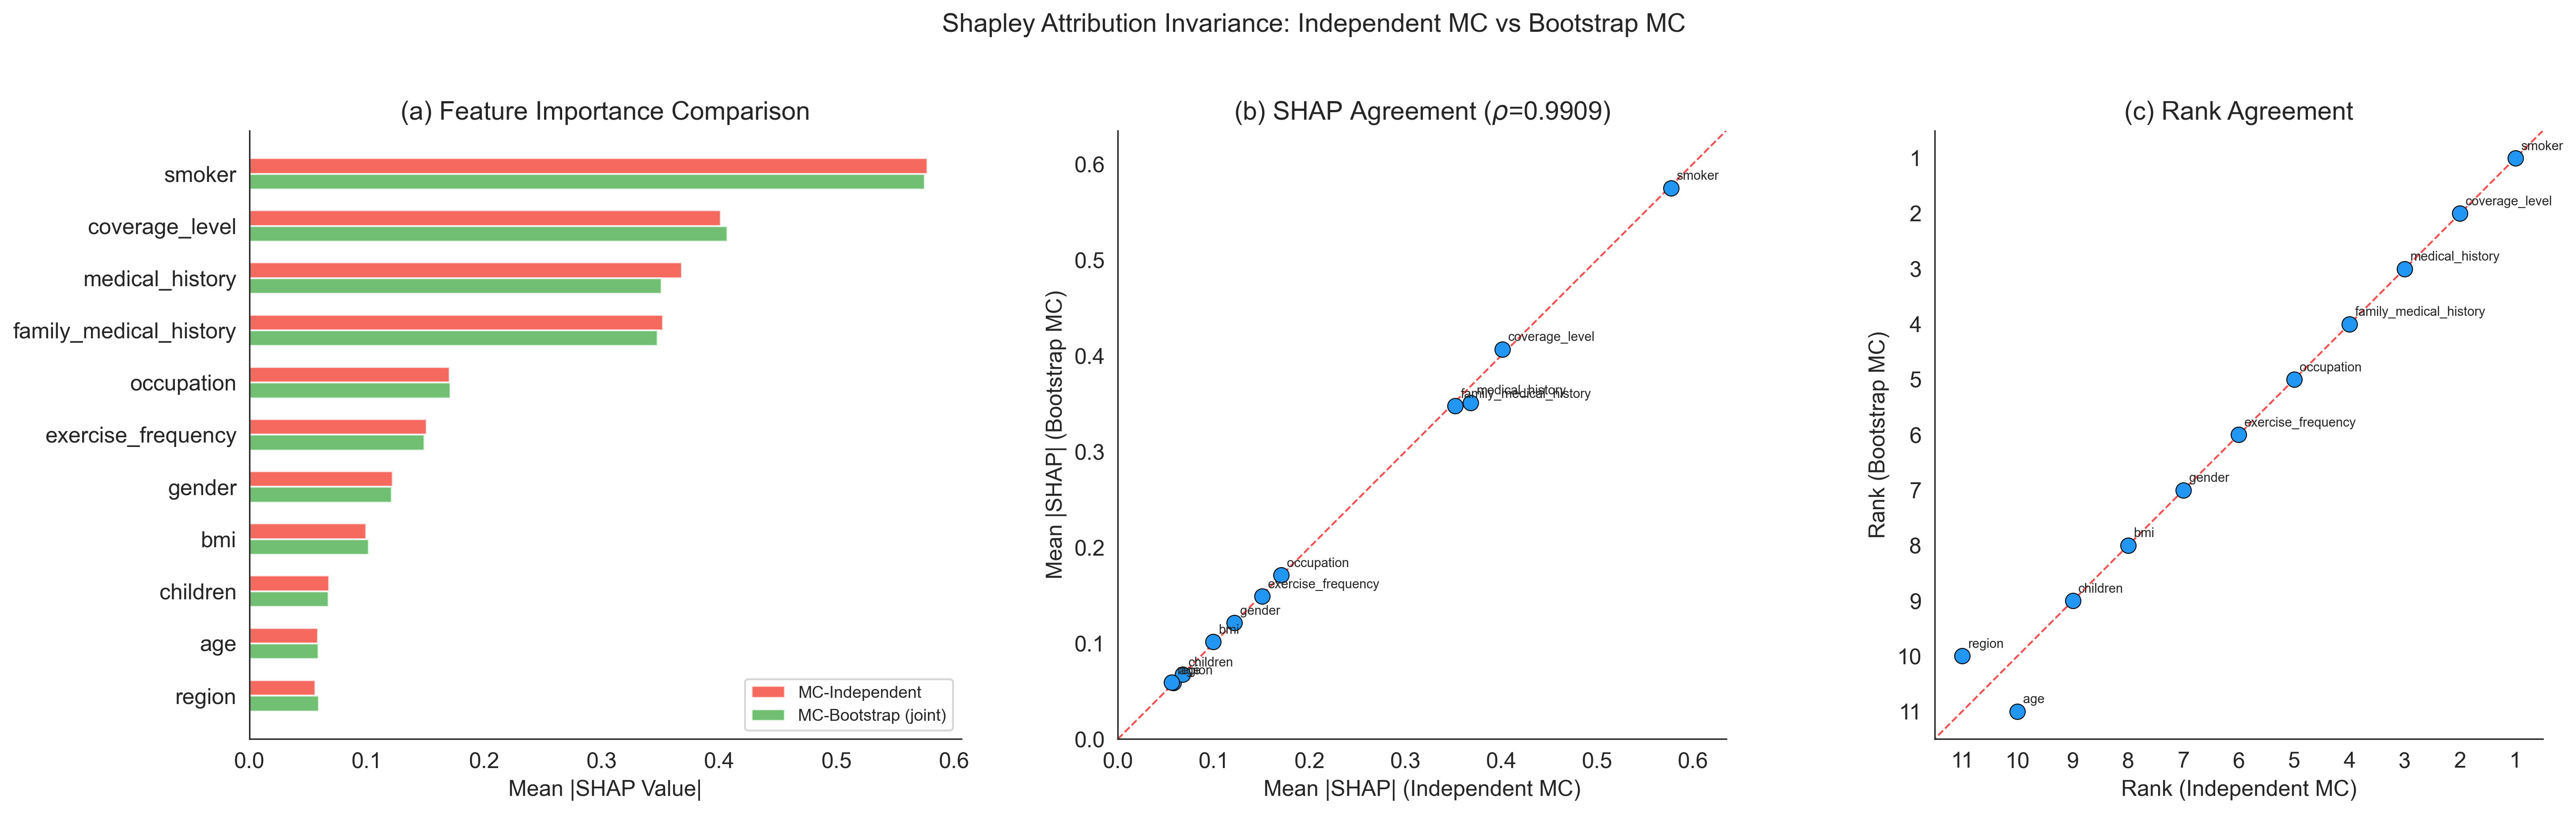
\includegraphics[width=0.95\textwidth]{Thesis/Chapter 3/Figures/fig_shap_bootstrap_vs_independent_invariance.png}
\caption{Shapley attribution invariance: parametric \gls{mc} versus bootstrap \gls{mc} input regimes.}
\label{fig:shapley_invariance_comparison_ch3}
\end{figure}

\subsubsection{Interpretation and conclusion}

The joint-distribution diagnostics confirm that the parametric \gls{mc} sample
differs from the training data in its dependence structure: the parametric
sample has zero cross-variable association by construction, whereas the
training data carries weak but non-zero dependencies. However, the
magnitude of these differences is small. The correlation matrix differences
do not exceed 0.042 (Figure~\ref{fig:correlation_difference_heatmap_ch3}),
all Cram\'{e}r's $V$ values fall below 0.04
(Figure~\ref{fig:cramers_v_comparison_ch3}), and the \gls{pca} overlays show that
both datasets populate the same region of principal component space
(Figure~\ref{fig:pca_joint_overlay_ch3}). The Shapley invariance comparison
yields a Spearman rank correlation of $\rho_{\mathrm{S}} = 0.991$ between
the parametric and bootstrap attribution vectors
(Figure~\ref{fig:shapley_invariance_comparison_ch3}), with the
feature-importance ordering preserved for all but the two weakest
contributors.

Because the joint-distribution differences are small and the Shapley
attributions are invariant to the input dependence structure, the
product-marginal independence assumption in
Section~\ref{sec:mc_simulation_design} is a defensible modelling choice. It
does not introduce meaningful bias into the subsequent high-cost conditional
Shapley analysis. The fitted \gls{dnn}'s internal importance structure,
rather than the dependence pattern of the input profiles, determines the
attribution results.

% =============================================================
\subsection{Residual-Augmented MC Sensitivity Analysis}
\label{sec:residual_augmented_mc}

A second \gls{mc} design assesses sensitivity to fitted residual
variation. The base \gls{mc} design produces deterministic fitted
predictions. The residual-augmented design adds a residual component to the
predicted costs to examine how the simulated output distribution changes
when fitted model error is introduced. The perturbation operates in the
output space (predicted costs) rather than the input space (policyholder
covariates). This is appropriate because the primary concern is whether the
distributional conclusions drawn from the base \gls{mc} analysis are
sensitive to the magnitude of the fitted model's residual error, not to
misspecification of the input distributions.

\subsubsection{Fitted residual distribution}

Let $e_i = y_i - \widehat{y}_i$ denote the fitted residual on the original
response scale for observations in the residual estimation set
$\mathcal{S}_{\varepsilon}$, taken as the training partition. Using the
training set for residual estimation is appropriate in this context because
the residuals serve only to characterise the magnitude and distributional
shape of fitted prediction error for the sensitivity analysis, not to assess
out-of-sample generalisation performance. The centred
residuals are
\begin{equation}
    e_i^{c}
    =
    e_i - \bar{e},
    \qquad
    \bar{e}
    =
    \frac{1}{|\mathcal{S}_{\varepsilon}|}
    \sum_{i \in \mathcal{S}_{\varepsilon}}
    e_i.
    \label{eq:centered_residuals_ch3}
\end{equation}
\equationlistentry{Centred fitted residuals}
The empirical residual distribution is
$\widehat{F}_{\varepsilon}
=
|\mathcal{S}_{\varepsilon}|^{-1}
\sum_{i \in \mathcal{S}_{\varepsilon}}
\delta_{e_i^{c}}$,
where $\delta_{e_i^{c}}$ denotes a point mass at $e_i^{c}$. The residual
standard deviation is
\begin{equation}
    \widehat{\sigma}_{\varepsilon}
    =
    \sqrt{
    \frac{1}{|\mathcal{S}_{\varepsilon}|-1}
    \sum_{i \in \mathcal{S}_{\varepsilon}}
    \left(
        e_i - \bar{e}
    \right)^2
    }.
    \label{eq:residual_sd_ch3}
\end{equation}
\equationlistentry{Residual standard deviation}

\subsubsection{Residual-augmented simulation}

For each base \gls{mc} prediction $\widehat{Y}^{(b)}$, a residual draw is
sampled:
\begin{equation}
    \varepsilon^{(b)}
    \sim
    \widehat{F}_{\varepsilon},
    \qquad
    b=1,\ldots,B.
    \label{eq:residual_draw_ch3}
\end{equation}
\equationlistentry{Residual draw from empirical distribution}
The residual-augmented predicted cost is
\begin{equation}
    Y_{\mathrm{res}}^{(b)}
    =
    \widehat{Y}^{(b)}
    +
    \varepsilon^{(b)},
    \qquad
    b=1,\ldots,B.
    \label{eq:residual_augmented_prediction_ch3}
\end{equation}
\equationlistentry{Residual-augmented predicted cost}
Negative values are truncated at zero:
$Y_{\mathrm{res},+}^{(b)}
=
\max\{0,\, Y_{\mathrm{res}}^{(b)}\}$.

\subsubsection{Fixed residual perturbation check}

A fixed perturbation check assesses sensitivity to the magnitude of residual
augmentation:
\begin{equation}
    Y_{+}^{(b)}
    =
    \widehat{Y}^{(b)}
    +
    0.5\,\widehat{\sigma}_{\varepsilon},
    \qquad
    Y_{-}^{(b)}
    =
    \max
    \left\{
        0,\,
        \widehat{Y}^{(b)}
        -
        0.5\,\widehat{\sigma}_{\varepsilon}
    \right\}.
    \label{eq:fixed_residual_perturbation_ch3}
\end{equation}
\equationlistentry{Fixed residual perturbation sensitivity band}
This is a deterministic sensitivity band around the fitted \gls{dnn} predictions,
not a probabilistic uncertainty interval. The residual-augmented simulation is
interpreted as a sensitivity analysis based on fitted residual variability. It
does not account for parameter uncertainty, model uncertainty or
data-generating uncertainty.

\begin{table}[H]
\centering
\small
\renewcommand{\arraystretch}{1.15}
\begin{tabular}{p{0.32\textwidth}p{0.58\textwidth}}
\toprule
\textbf{Component} & \textbf{Specification} \\
\midrule
Base prediction & $\widehat{Y}^{(b)} = \widehat{m}(\mathbf{z}^{(b)})$ \\
Residual source & Fitted residuals from the training partition \\
Residual centring & Residuals centred before resampling \\
Main residual design & $\varepsilon^{(b)} \sim \widehat{F}_{\varepsilon}$ \\
Residual-augmented output & $Y_{\mathrm{res}}^{(b)} = \widehat{Y}^{(b)}+\varepsilon^{(b)}$ \\
Fixed perturbation check & $\widehat{Y}^{(b)} \pm 0.5\,\widehat{\sigma}_{\varepsilon}$ \\
Non-negativity rule & Negative simulated costs truncated at zero \\
\bottomrule
\end{tabular}
\caption{Residual-augmented \gls{mc} sensitivity design.}
\label{tab:residual_augmented_design_ch3}
\end{table}

\begin{table}[H]
\centering
\small
\renewcommand{\arraystretch}{1.15}
\begin{tabular}{p{0.92\textwidth}}
\toprule
\textbf{Algorithm 3.2: Residual-augmented \gls{mc} sensitivity simulation} \\
\midrule
\textbf{Input:} base \gls{mc} predictions
$\{\widehat{Y}^{(b)}\}_{b=1}^{B}$, fitted residual distribution
$\widehat{F}_{\varepsilon}$, residual standard deviation
$\widehat{\sigma}_{\varepsilon}$, random seed $s$. \\[3pt]

\textbf{Output:} residual-augmented outputs
$\{Y_{\mathrm{res}}^{(b)}\}_{b=1}^{B}$, upper perturbation outputs
$\{Y_{+}^{(b)}\}_{b=1}^{B}$, and lower perturbation outputs
$\{Y_{-}^{(b)}\}_{b=1}^{B}$. \\[3pt]

1. Set the random seed to $s$. \\
2. Estimate residuals $e_i = y_i-\widehat{y}_i$ on the residual estimation set. \\
3. Centre the residuals and construct $\widehat{F}_{\varepsilon}$. \\
4. For $b=1,\ldots,B$, draw $\varepsilon^{(b)} \sim \widehat{F}_{\varepsilon}$. \\
5. Calculate $Y_{\mathrm{res}}^{(b)} = \widehat{Y}^{(b)}+\varepsilon^{(b)}$. \\
6. Apply the non-negativity rule if required. \\
7. Calculate the fixed perturbation outputs $Y_{+}^{(b)}$ and $Y_{-}^{(b)}$. \\
8. Store all outputs for comparison with the base \gls{mc} distribution. \\
\bottomrule
\end{tabular}
\caption{Residual-augmented \gls{mc} algorithm.}
\label{tab:residual_augmented_algorithm_ch3}
\end{table}


% =============================================================
\subsection{Shapley-Value Attribution for Simulated Profiles}
\label{sec:shapley_attribution_simulated_profiles}
\label{sec:shapley_interpretation_design}
\label{sec:high_cost_conditional_shapley}

Shapley-value methods are used to explain the fitted \gls{dnn} predictions
calculated for simulated policyholder profiles. The attribution analysis is
connected to the \gls{mc} predicted-cost distribution, with particular
attention to the upper tail.

\subsubsection{Prediction function and Shapley decomposition}

The prediction function supplied to \gls{shap} is the fitted \gls{dnn}
together with the response de-normalisation step. Shapley values are
therefore reported on the original monetary scale of \texttt{charges}. For a
simulated model-ready profile $\mathbf{z}^{(b)}$, the fitted prediction is
decomposed following equation~\eqref{eq:shapley_decomp}, with $p = 22$
encoded features. The baseline prediction $\phi_0$ and the feature-level
contributions $\phi_j(\mathbf{z}^{(b)})$ are defined exactly as in
Section~\ref{sec:explainability_shapley_shap}.

\subsubsection{Implementation settings}

The background data are sampled from the model-ready training partition. The
primary implementation uses a gradient-based \gls{shap} explainer for the
differentiable \gls{dnn}. A model-agnostic KernelSHAP calculation may be
applied to a small validation subset as a computational check if required.

The gradient-based \gls{shap} explainer computes
approximate Shapley values, not exact game-theoretic Shapley
values.  Exact computation requires evaluating the prediction function at
all $2^p$ feature subsets, which is computationally infeasible for $p = 22$
encoded features ($2^{22} = 4\,194\,304$ coalition evaluations per
profile).  The gradient-based approximation leverages the differentiability
of the fitted \gls{dnn} to estimate feature contributions efficiently, but
the resulting attributions are conditional on the background sample, the
explainer algorithm, and the fitted network parameters.  All reported
Shapley values should therefore be interpreted as model-specific,
approximate attributions rather than exact cooperative-game solutions.

\begin{table}[H]
\centering
\small
\renewcommand{\arraystretch}{1.15}
\begin{tabular}{p{0.32\textwidth}p{0.58\textwidth}}
\toprule
\textbf{Item} & \textbf{Specification} \\
\midrule
Prediction function & Fitted \gls{dnn} with response de-normalisation \\
Output scale & Original monetary scale of \texttt{charges} \\
Explainer & Gradient-based \gls{shap} explainer \\
Background data & Sample from the model-ready training partition \\
Background size & $m_0 = 200$ observations, selected as the largest size that maintains computational feasibility for the gradient-based explainer \\
Explained profiles & \gls{mc} simulated profiles $\mathbf{z}^{(b)}$ \\
Primary summaries & Mean signed and mean absolute Shapley values \\
Conditional summaries & Shapley summaries for upper-tail simulated profiles \\
Categorical treatment & Dummy-level attributions aggregated to raw-variable level \\
\bottomrule
\end{tabular}
\caption{\Gls{shap} implementation settings.}
\label{tab:shap_implementation_settings_ch3}
\end{table}

\subsubsection{Aggregation from encoded inputs to raw variables}

The fitted \gls{dnn} receives $p = 22$ encoded features, but some columns are
dummy variables derived from a single raw categorical predictor. If $G_g$
denotes the set of encoded columns associated with raw variable $g$, the
raw-variable Shapley contribution is
\begin{equation}
    \Phi_g
    \left(
        \mathbf{z}^{(b)}
    \right)
    =
    \sum_{j \in G_g}
    \phi_j
    \left(
        \mathbf{z}^{(b)}
    \right).
    \label{eq:raw_variable_shap_aggregation_ch3}
\end{equation}
\equationlistentry{Raw-variable Shapley aggregation from encoded inputs}
This aggregation prevents the interpretation from being fragmented across
several dummy columns belonging to the same original variable.

The four Shapley axioms that uniquely characterise the Shapley value
\citep{shapley1953value} were discussed in
Section~\ref{sec:explainability_shapley_shap}.  In the present context, the
efficiency, symmetry, dummy, and additivity properties ensure that the
aggregation from encoded features to raw variables is a linear
repartitioning that preserves the complete decomposition.  The raw-variable
contributions $\Phi_g$ therefore retain the same axiomatic guarantees as the
underlying feature-level values $\phi_j$, and the total prediction remains
fully decomposed into $q = 11$ raw-variable contributions without remainder.

\subsubsection{Global Shapley summaries}

Shapley values are computed for all $B$ simulated profiles generated in the
base \gls{mc} simulation, so $B_{\mathrm{shap}} = B$. Global feature
importance $I_j$ follows the mean absolute Shapley value defined in
Section~\ref{sec:explainability_shapley_shap}, computed over the simulated
profiles. A mean signed summary is also reported.
The mean signed Shapley contribution for feature $j$ is
\begin{equation}
    \overline{\phi}_{j}
    =
    \frac{1}{B_{\mathrm{shap}}}
    \sum_{b=1}^{B_{\mathrm{shap}}}
    \phi_j
    \left(
        \mathbf{z}^{(b)}
    \right),
    \label{eq:mean_signed_shap_ch3}
\end{equation}
\equationlistentry{Mean signed Shapley contribution}
and the mean absolute Shapley contribution is
\begin{equation}
    I_j
    =
    \frac{1}{B_{\mathrm{shap}}}
    \sum_{b=1}^{B_{\mathrm{shap}}}
    \left|
        \phi_j
        \left(
            \mathbf{z}^{(b)}
        \right)
    \right|.
    \label{eq:mean_absolute_shap_ch3}
\end{equation}
\equationlistentry{Mean absolute Shapley contribution (feature importance)}
The signed summary describes the average direction of the contribution; the
absolute summary measures average magnitude.

\subsubsection{High-cost region and conditional Shapley summaries}

The high-cost region is defined using the quantile-based threshold
$u_{\tau}$ from equation~\eqref{eq:high_cost_threshold} and the
high-cost set $\mathcal{H}_{\tau}$ from
equation~\eqref{eq:high_cost_set}, applied to the $B$ simulated profiles
with $\tau \in \{0.90, 0.95, 0.99\}$.
The 95th percentile is used as the main high-cost threshold because it
balances two competing requirements: it retains a sufficient number of
upper-tail profiles ($|H_{0.95}| = 0.05B$) for stable conditional Shapley
averages, while still isolating profiles that represent genuinely high
predicted costs. The 90th and 99th percentiles are retained as sensitivity
thresholds to assess whether the attribution patterns are robust to the
choice of cutoff. The conditional mean signed contribution
$\overline{\phi}_{j,\tau}$ and the conditional mean absolute contribution
$I_{j,\tau}$ are computed as in
equations~\eqref{eq:signed_shapley_high}
and~\eqref{eq:abs_shapley_high}, with the high-cost set
$\mathcal{H}_{\tau}$ replacing the generic conditioning set and the
summation taken over the $B$ simulated profiles. These conditional
summaries are also aggregated to the raw-variable level using
equation~\eqref{eq:raw_variable_shap_aggregation_ch3}.
Comparing $I_j$ with $I_{j,\tau}$ shows whether a feature is generally
important across all simulated profiles or specifically important in the
high-cost region. For the residual-augmented simulation, a separate high-cost
set can be defined using the residual-augmented outputs to examine whether the
profiles classified as high cost change when fitted residual variability is
introduced. Since the residual component is added after the fitted \gls{dnn}
prediction, Shapley values explain the fitted \gls{dnn} component
$\widehat{m}(\mathbf{z}^{(b)})$ rather than the residual addition.

\subsubsection{Bootstrap confidence intervals for conditional Shapley values}

At $\tau_{99}$ the conditioning set contains only $|\mathcal{H}_{0.99}| = 0.01B$ profiles, so the conditional mean absolute Shapley values are estimated from a small effective sample. To quantify estimation uncertainty, a nonparametric bootstrap is applied. Let $\boldsymbol{\Phi}_{\tau} \in \mathbb{R}^{|\mathcal{H}_{\tau}| \times q}$ denote the matrix of raw-variable Shapley values for profiles in $\mathcal{H}_{\tau}$. The bootstrap procedure is:

\begin{enumerate}
    \item Draw $R = 10\,000$ bootstrap resamples $\boldsymbol{\Phi}_{\tau}^{*(r)}$, each of size $|\mathcal{H}_{\tau}|$, with replacement from $\boldsymbol{\Phi}_{\tau}$.
    \item For each resample $r$, compute the mean absolute Shapley value for each variable:
    \[
        I_{j,\tau}^{*(r)} = \frac{1}{|\mathcal{H}_{\tau}|} \sum_{i=1}^{|\mathcal{H}_{\tau}|} \bigl|\phi_{ij}^{*(r)}\bigr|, \qquad j = 1, \ldots, q.
    \]
    \item The 95\% bootstrap confidence interval for $I_{j,\tau}$ is the interval $\bigl[I_{j,\tau}^{*(0.025)},\; I_{j,\tau}^{*(0.975)}\bigr]$, where $I_{j,\tau}^{*(\alpha)}$ is the $\alpha$-quantile of the bootstrap distribution $\{I_{j,\tau}^{*(1)}, \ldots, I_{j,\tau}^{*(R)}\}$.
\end{enumerate}

This percentile bootstrap is reported alongside the conditional importance values at $\tau_{99}$ in Chapter~\ref{sec:results}.

\begin{table}[H]
\centering
\small
\renewcommand{\arraystretch}{1.15}
\begin{tabular}{p{0.30\textwidth}p{0.60\textwidth}}
\toprule
\textbf{Summary} & \textbf{Purpose} \\
\midrule
Mean signed Shapley value & Average directional effect on fitted predictions \\
Mean absolute Shapley value & Average contribution magnitude across simulated profiles \\
Raw-variable aggregated Shapley value & Combines dummy-level attributions into original variables \\
High-cost conditional Shapley value & Identifies drivers of upper-tail predicted costs \\
Threshold comparison & Compares attribution at 90th, 95th and 99th percentiles \\
Base versus residual high-cost sets & Checks whether residual augmentation changes high-cost membership \\
\bottomrule
\end{tabular}
\caption{Shapley summaries calculated for simulated profiles.}
\label{tab:shap_summaries_ch3}
\end{table}


% =============================================================
\subsection{Modelling Assumptions}
\label{sec:modelling_assumptions}

The empirical framework depends on the modelling assumptions stated in
Table~\ref{tab:modelling_assumptions_ch3}. These assumptions define the
boundary of the empirical claims: the analysis can support statements about
how the fitted \gls{dnn} behaves on the benchmark dataset and under the stated Monte
Carlo input assumptions, but cannot, without external validation, support
causal claims about healthcare expenditure.

\begin{table}[H]
\centering
\small
\renewcommand{\arraystretch}{1.16}
\begin{tabular}{p{0.06\textwidth}p{0.25\textwidth}p{0.59\textwidth}}
\toprule
\textbf{No.} & \textbf{Assumption} & \textbf{Interpretation} \\
\midrule
A1 &
Benchmark data &
The dataset is a public benchmark and not a representative insurer portfolio \\

A2 &
Training-set preprocessing &
Encoding, numerical scaling and response scaling are estimated from the training set and applied unchanged elsewhere \\

A3 &
Bias-free \gls{dnn} &
The constrained architecture is assessed empirically through validation and test diagnostics \\

A4 &
No explicit regularisation &
Generalisation is assessed using validation behaviour, held-out performance and structural diagnostics \\

A5 &
Raw-variable \gls{mc} simulation &
Synthetic profiles are generated at the raw variable level and only then encoded \\

A6 &
Product-marginal input distribution &
The joint \gls{mc} input law is a practical simulation assumption and not a proof of covariate independence; validated by joint-distribution diagnostics and Shapley invariance comparison (Section~\ref{sec:mc_input_validation}) \\

A7 &
Joint-distribution validation &
The Shapley attributions are shown to be invariant to whether input profiles preserve training-data dependencies (bootstrap \gls{mc}) or assume full independence (parametric \gls{mc}) \\

A8 &
Base \gls{mc} interpretation &
The base simulated output distribution represents \gls{dnn} fitted predictions under the stated input assumptions, not realised healthcare costs \\

A9 &
Residual augmentation &
Residual-augmented simulation is a sensitivity analysis and not a complete predictive uncertainty model \\

A10 &
Shapley interpretation &
Shapley values explain the fitted \gls{dnn} predictions and are not causal feature effects \\

A11 &
High-cost definition &
High-cost profiles are defined by empirical upper-tail quantiles of the simulated predicted-cost distribution \\
\bottomrule
\end{tabular}
\caption{Summary of modelling assumptions and interpretive boundaries.}
\label{tab:modelling_assumptions_ch3}
\end{table}

With the data, architecture, simulation design, attribution method and
modelling assumptions now fully specified, the empirical results of the
three-stage framework are presented in Chapter~\ref{sec:results}.



% =============================================================
% Chapter 4: Results
% =============================================================
\clearpage
% =============================================================
% Chapter 4: Results
% =============================================================
\section{Results}
\label{sec:results}

This chapter presents the empirical results of the three-component
methodological pipeline specified in Chapter~\ref{chap:methods_and_data}.
The results are organised as follows:
Section~\ref{sec:hyperparameter_results} reports the sequential
hyperparameter comparison that produced the final \gls{dnn} training
configuration, together with the predictive performance of the retained
model and a baseline comparison with the actuarial-standard \gls{glm};
Section~\ref{sec:mc_results} presents the Monte Carlo
predicted-cost distribution, its joint-distribution input validation,
and convergence properties;
Section~\ref{sec:residual_augmented_results} evaluates the
residual-augmented sensitivity analysis;
Section~\ref{sec:shapley_results} reports the Shapley-value attribution
results at the global and high-cost conditional levels; and
Section~\ref{sec:mc_shapley_integration} examines the correspondence
between the Monte Carlo distributional findings and the Shapley
attribution patterns.


% =============================================================
\subsection{Hyperparameter Comparison Results}
\label{sec:hyperparameter_results}

The five-phase sequential hyperparameter comparison
(Section~\ref{sec:dnn_specification_training}) was carried out on the
architecture specified in Figure~\ref{fig:dnn_architecture_ch3}.
The results of each phase are presented below.

\subsubsection{Phase 1: Activation function}

Three candidate activation functions were compared: \gls{celu}
(equation~\eqref{eq:celu}), GELU and Tanh, with all other
hyperparameters fixed at learning rate $0.001$, batch size $256$ and Adam.

\begin{figure}[H]
\centering
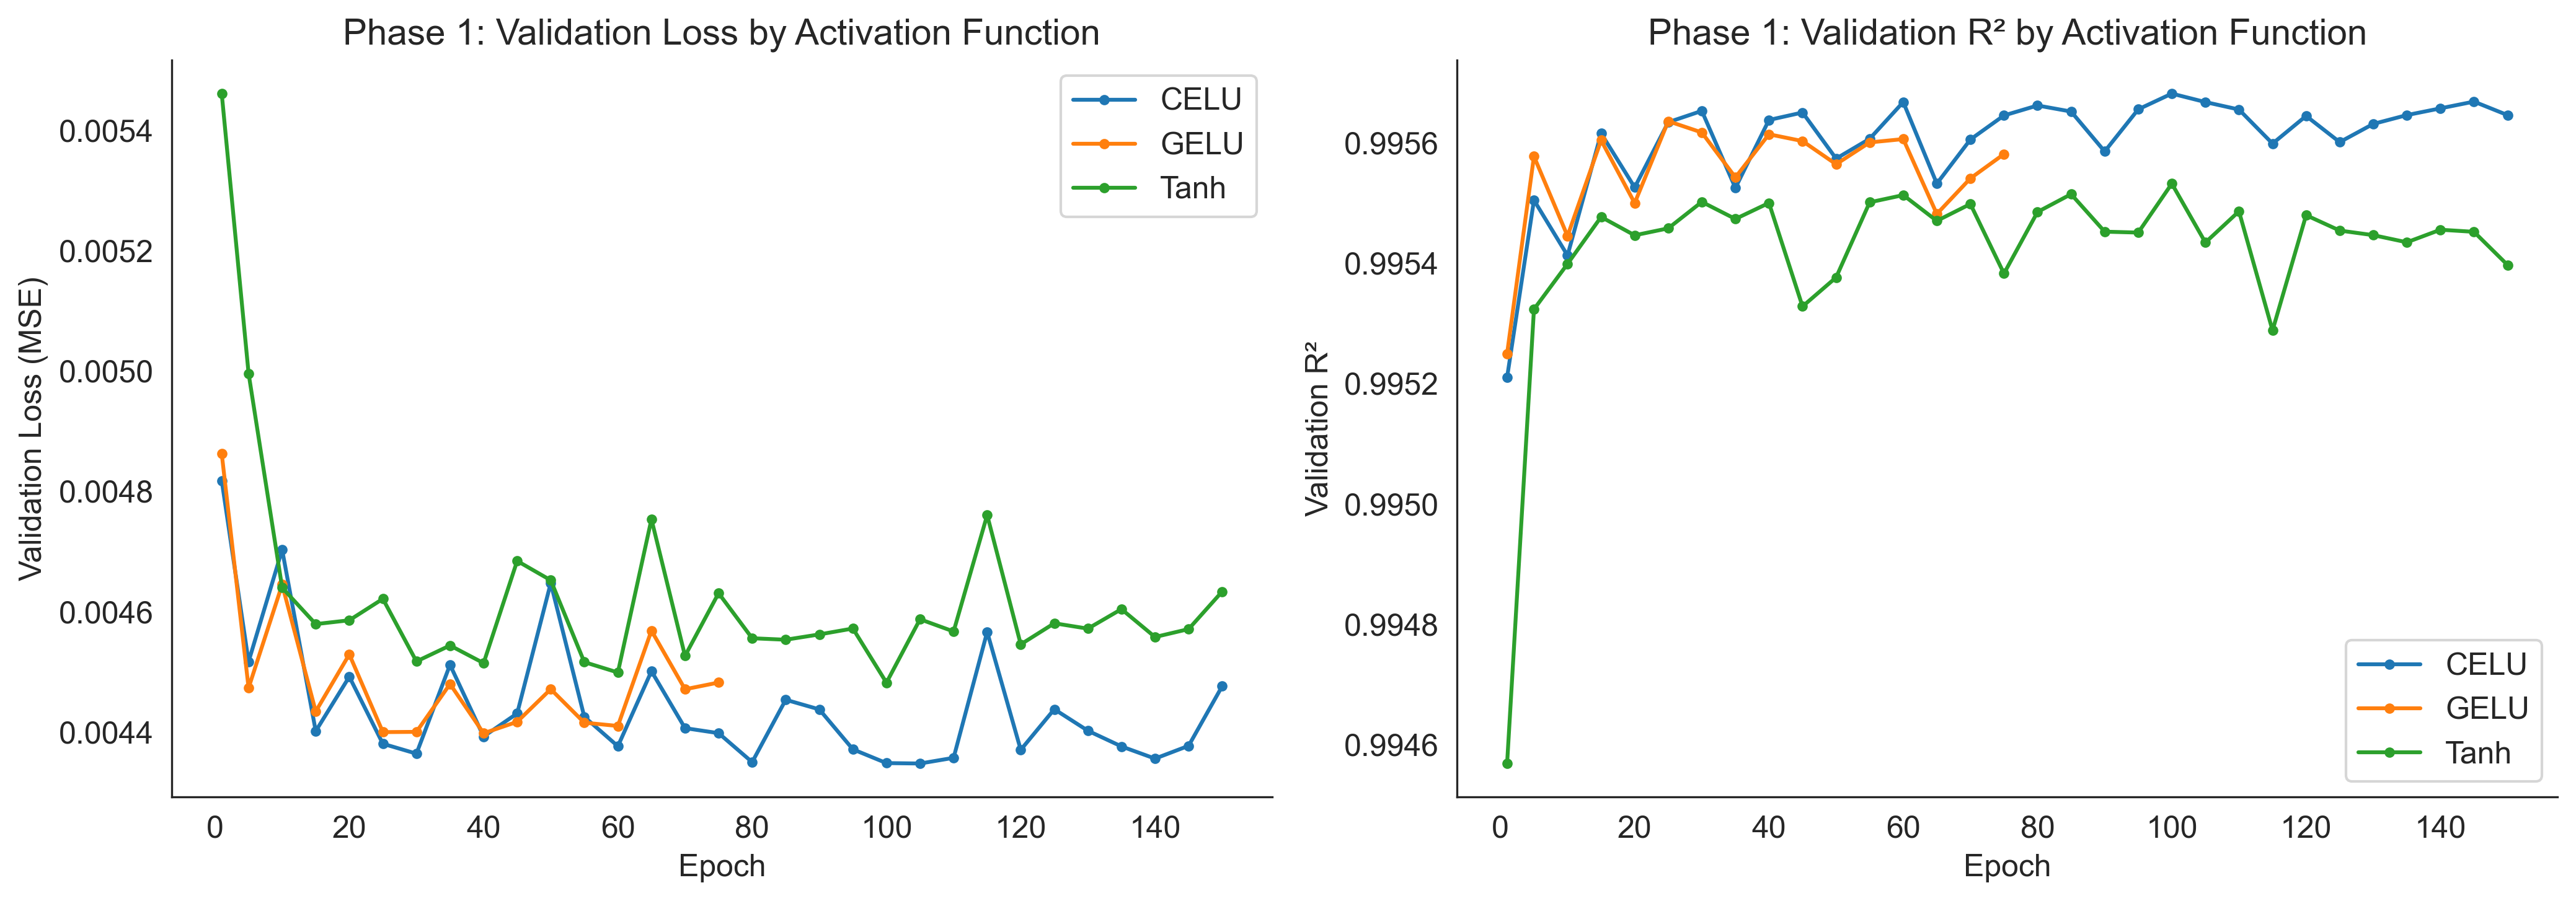
\includegraphics[width=0.95\textwidth]{Thesis/Chapter 4/Figures/fig_phase1_activation_comparison.png}
\caption{Phase~1: validation MSE loss (left) and validation $R^2$
(right) by activation function over training epochs.}
\label{fig:phase1_activation_ch4}
\end{figure}

\noindent
Figure~\ref{fig:phase1_activation_ch4} shows that \gls{celu} achieves
the lowest validation loss (approximately $0.00435$) and the highest
validation $R^2$ (approximately $0.9957$) from epoch~60 onwards. GELU
tracks \gls{celu} closely throughout training but settles at a
marginally higher loss plateau. Tanh converges more slowly and exhibits
greater epoch-to-epoch volatility, reaching a best validation $R^2$ of
approximately $0.9954$. The \gls{celu} activation was therefore retained.

\subsubsection{Phase 2: Learning rate}

Four learning rates were evaluated:
$\eta \in \{0.01, 0.001, 0.0005, 0.0001\}$, with \gls{celu} carried
forward.

\begin{figure}[H]
\centering
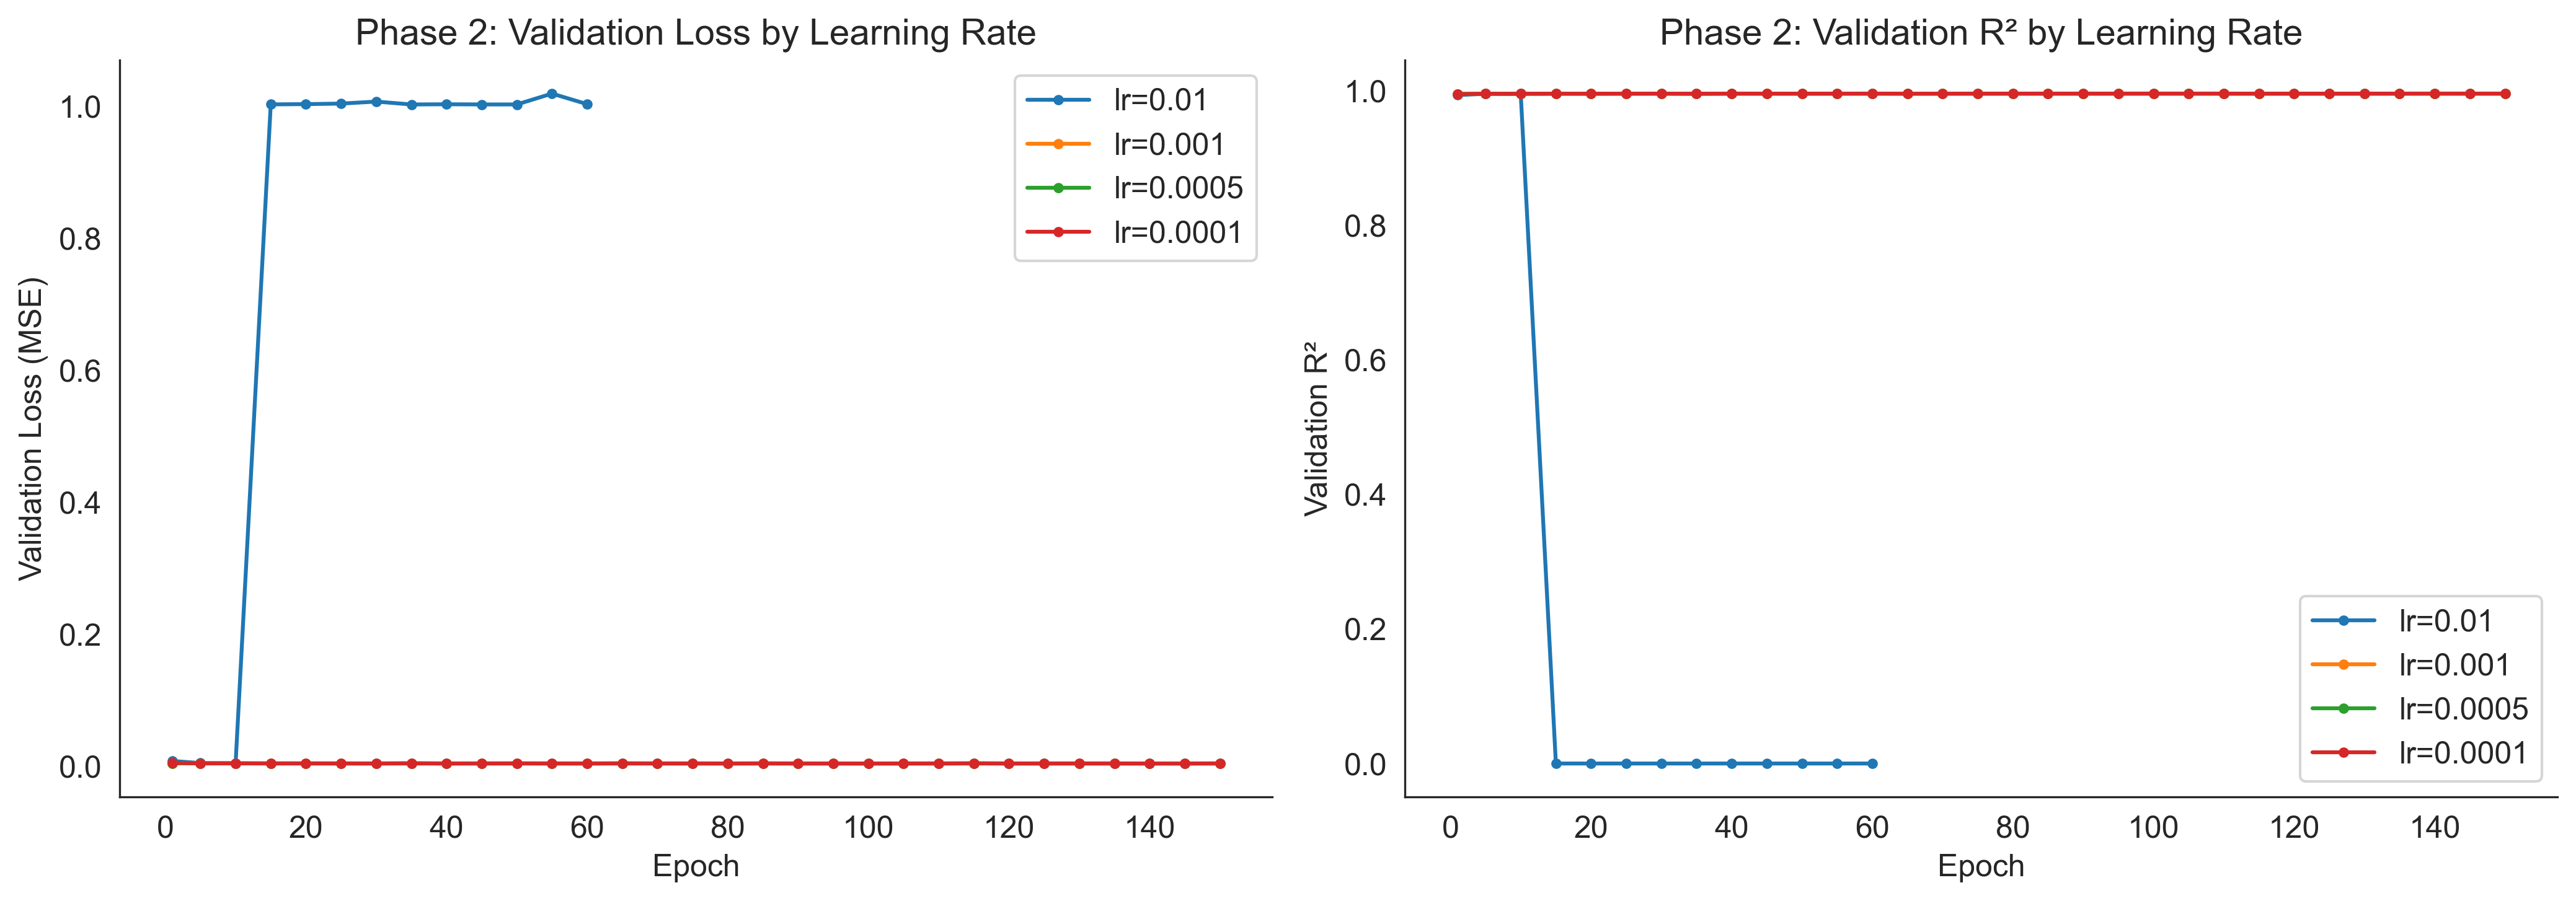
\includegraphics[width=0.95\textwidth]{Thesis/Chapter 4/Figures/fig_phase2_lr_comparison.png}
\caption{Phase~2: validation MSE loss (left) and validation $R^2$
(right) by learning rate.}
\label{fig:phase2_lr_ch4}
\end{figure}

\noindent
Figure~\ref{fig:phase2_lr_ch4} reveals that $\eta = 0.01$ produces
catastrophic divergence: the validation loss exceeds $1.0$ and the
validation $R^2$ drops to near zero, indicating that the gradient
updates overshoot the loss surface at this step size. The three
remaining learning rates ($0.001$, $0.0005$ and $0.0001$) all converge
to validation $R^2 \approx 1.00$ on the standardised scale, with their
loss curves overlapping on the visible scale. Among these,
$\eta = 0.0005$ achieves the lowest best validation loss and was
retained.

\subsubsection{Phase 3: Batch size}

Four batch sizes were compared:
$|\mathcal{B}| \in \{64, 128, 256, 512\}$, with \gls{celu} and
$\eta = 0.0005$ fixed.

\begin{figure}[H]
\centering
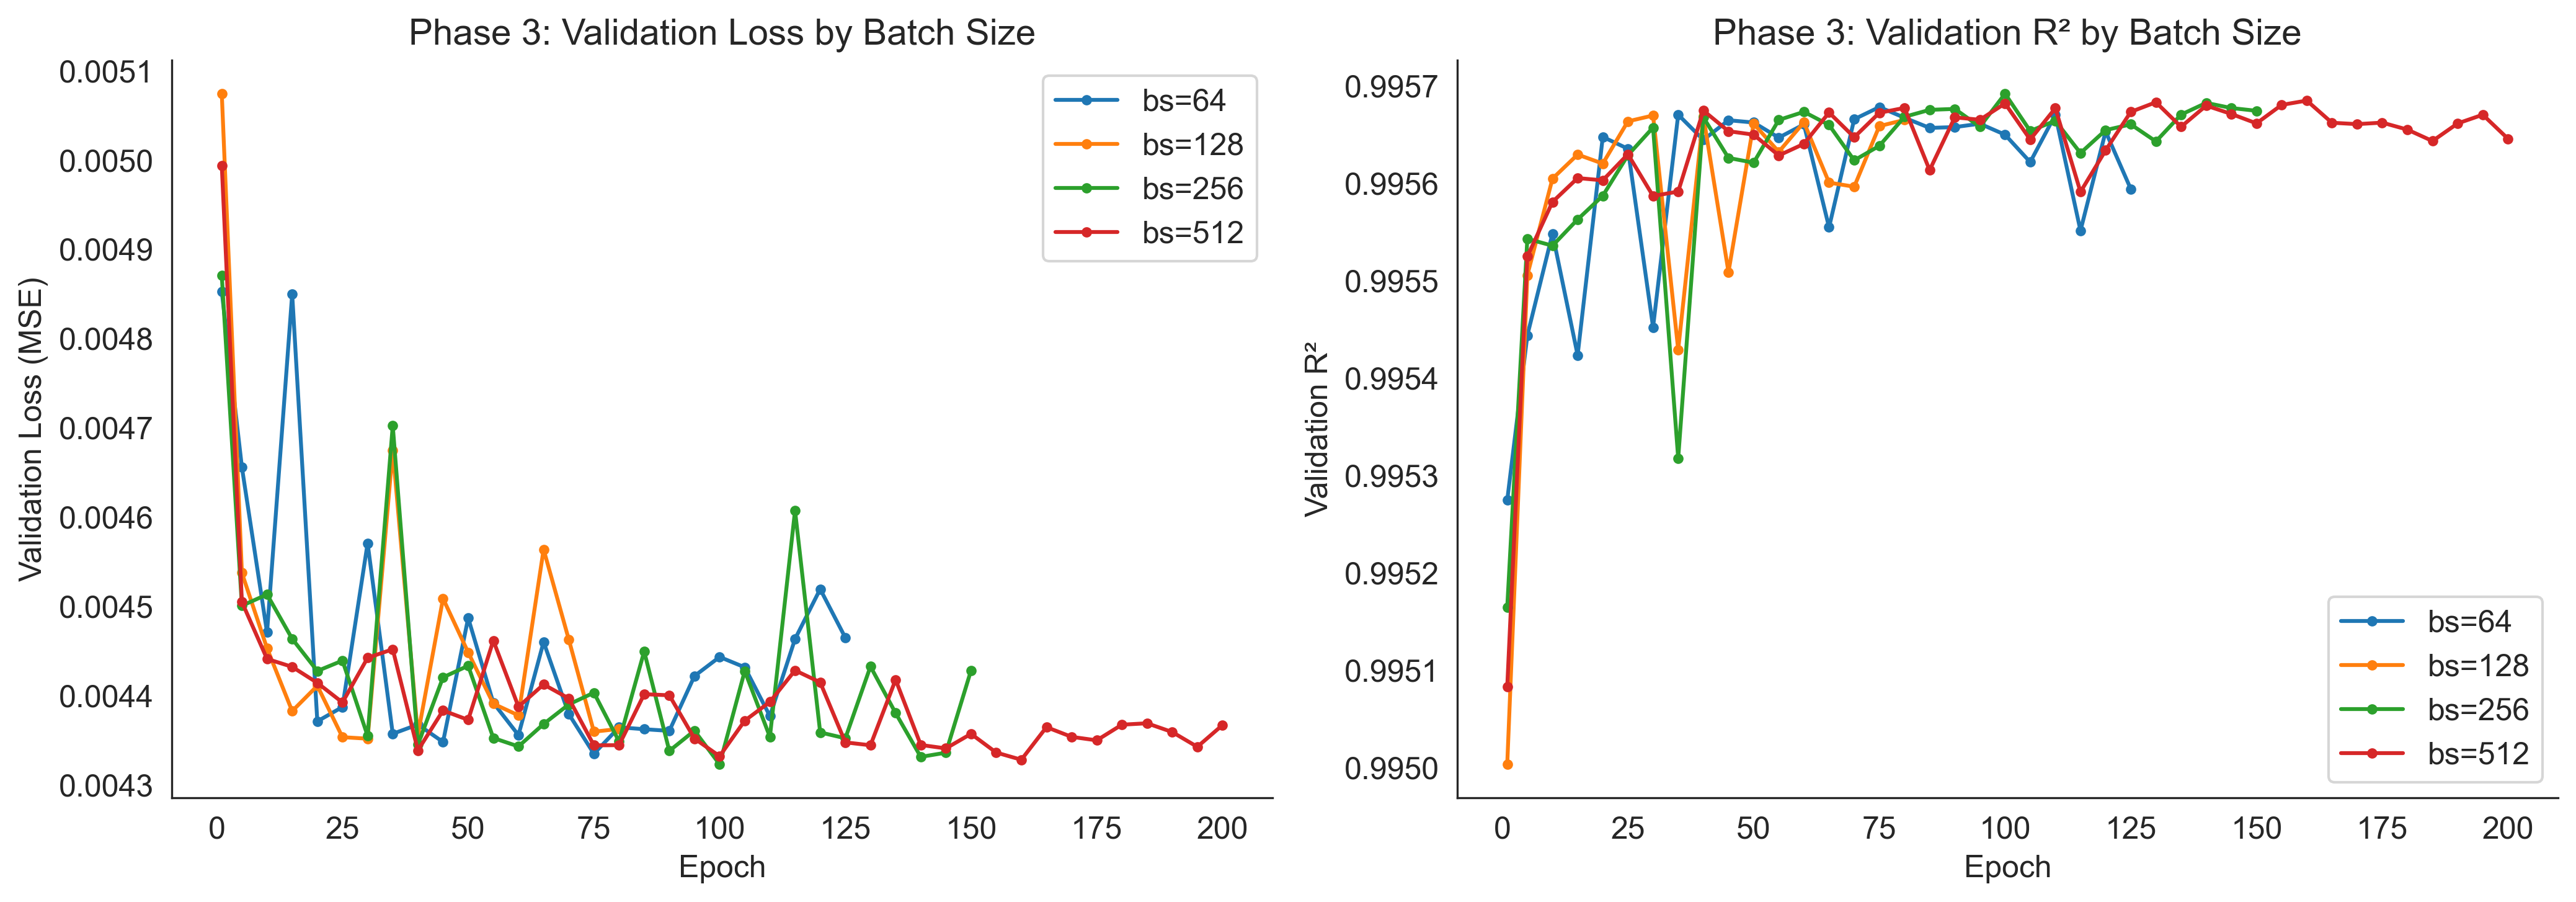
\includegraphics[width=0.95\textwidth]{Thesis/Chapter 4/Figures/fig_phase3_batchsize_comparison.png}
\caption{Phase~3: validation MSE loss (left) and validation $R^2$
(right) by batch size.}
\label{fig:phase3_batchsize_ch4}
\end{figure}

\noindent
Figure~\ref{fig:phase3_batchsize_ch4} shows that all four batch sizes
converge to similar validation performance, with best validation $R^2$
values between $0.9956$ and $0.9957$. The batch size $|\mathcal{B}| =
256$ was retained, as it achieves among the lowest validation loss
values while maintaining stable convergence behaviour.

\subsubsection{Phase 4: Optimiser}

Adam and Nadam were compared with all previous best choices carried
forward.

\begin{figure}[H]
\centering
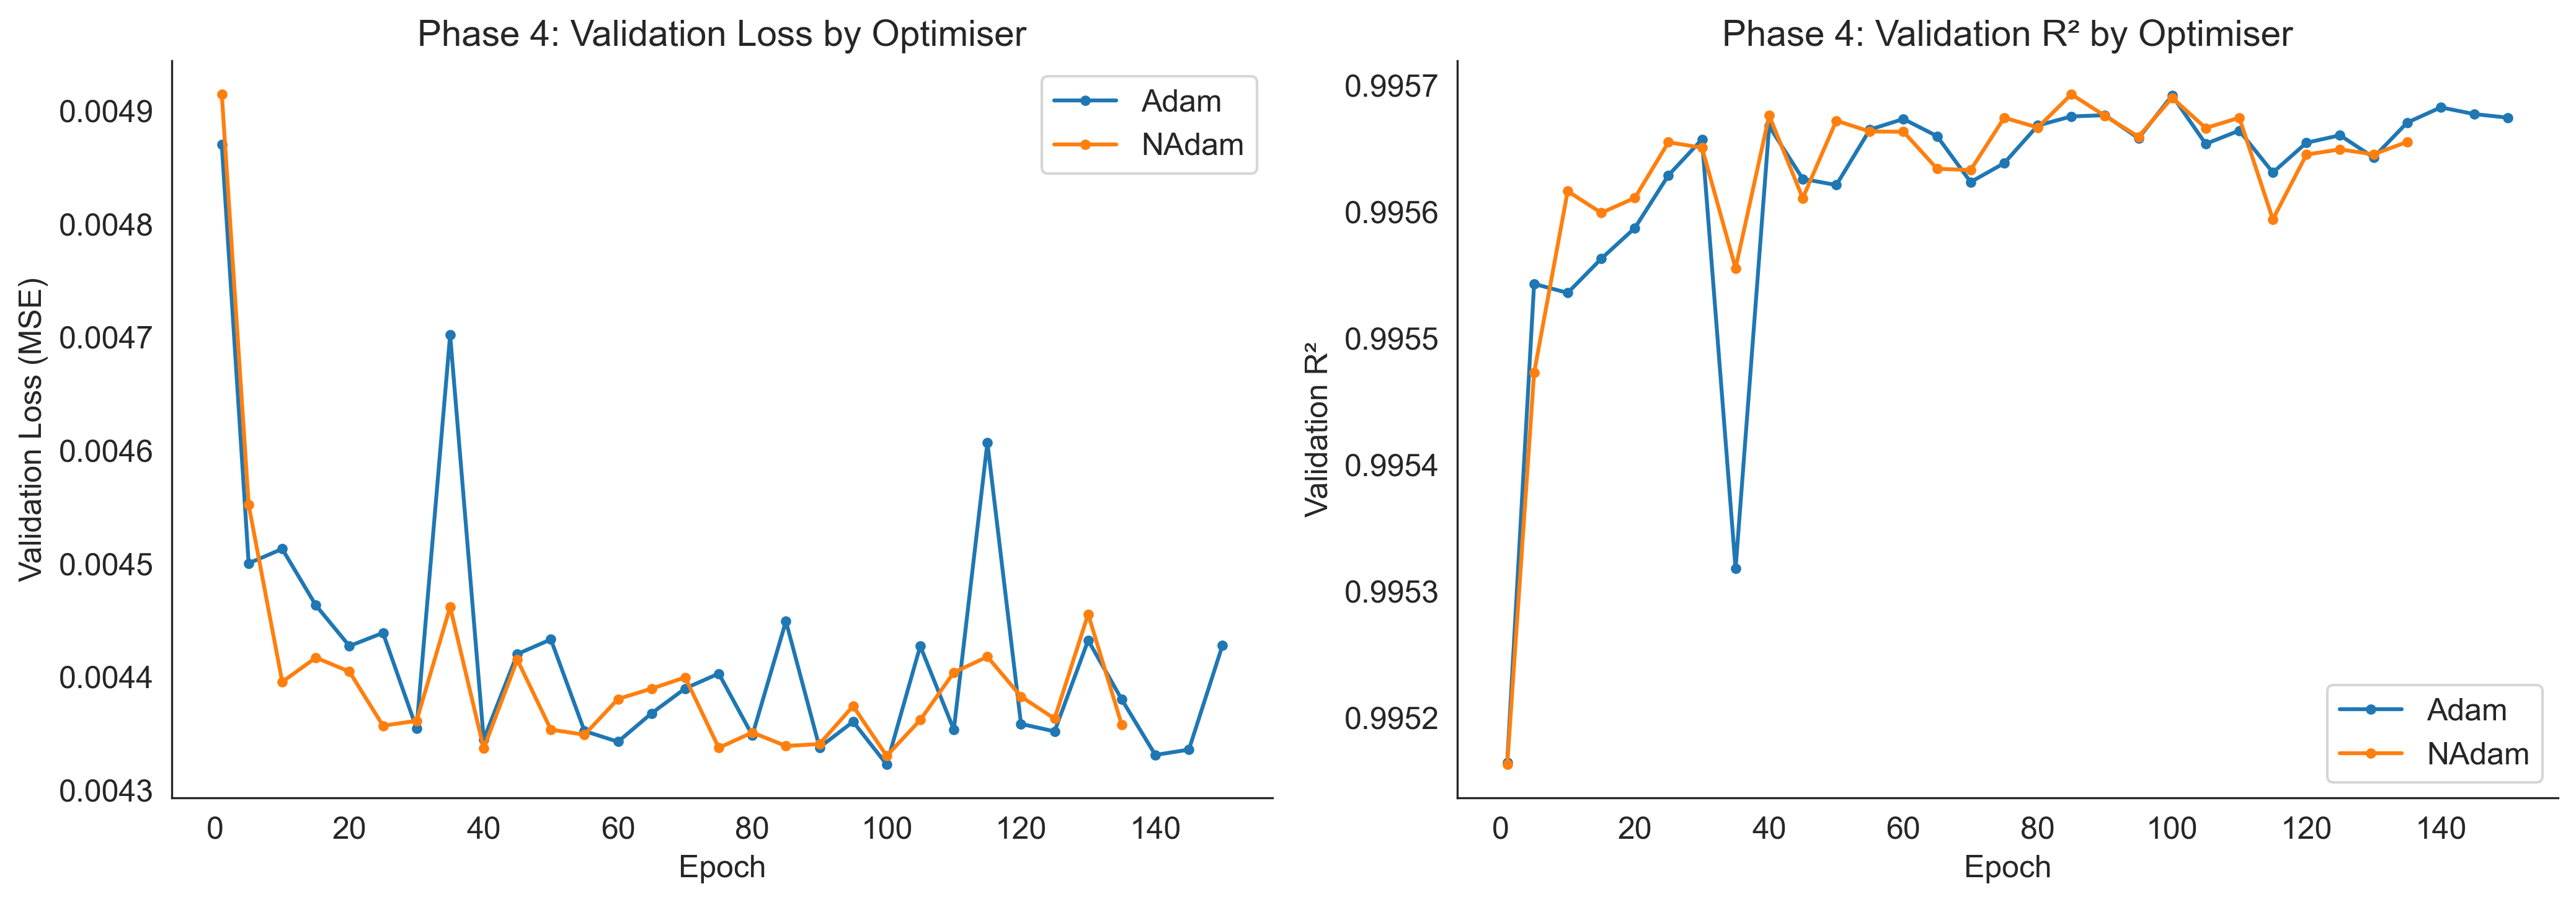
\includegraphics[width=0.95\textwidth]{Thesis/Chapter 4/Figures/fig_phase4_optimiser_comparison.png}
\caption{Phase~4: validation MSE loss (left) and validation $R^2$
(right) by optimiser.}
\label{fig:phase4_optimiser_ch4}
\end{figure}

\noindent
Figure~\ref{fig:phase4_optimiser_ch4} shows that Nadam converges faster
than Adam in the initial epochs and exhibits smoother validation loss
trajectories throughout training. From approximately epoch~40 onwards,
Nadam consistently achieves lower validation loss and higher validation
$R^2$ than Adam, with fewer loss spikes. Nadam was therefore retained.

\subsubsection{Phase 5: Momentum parameters}

Three momentum configurations were compared for the Nadam optimiser:
$(\beta_1, \beta_2) \in \{(0.90, 0.999),\; (0.95, 0.999),\;
(0.99, 0.999)\}$.

\begin{figure}[H]
\centering
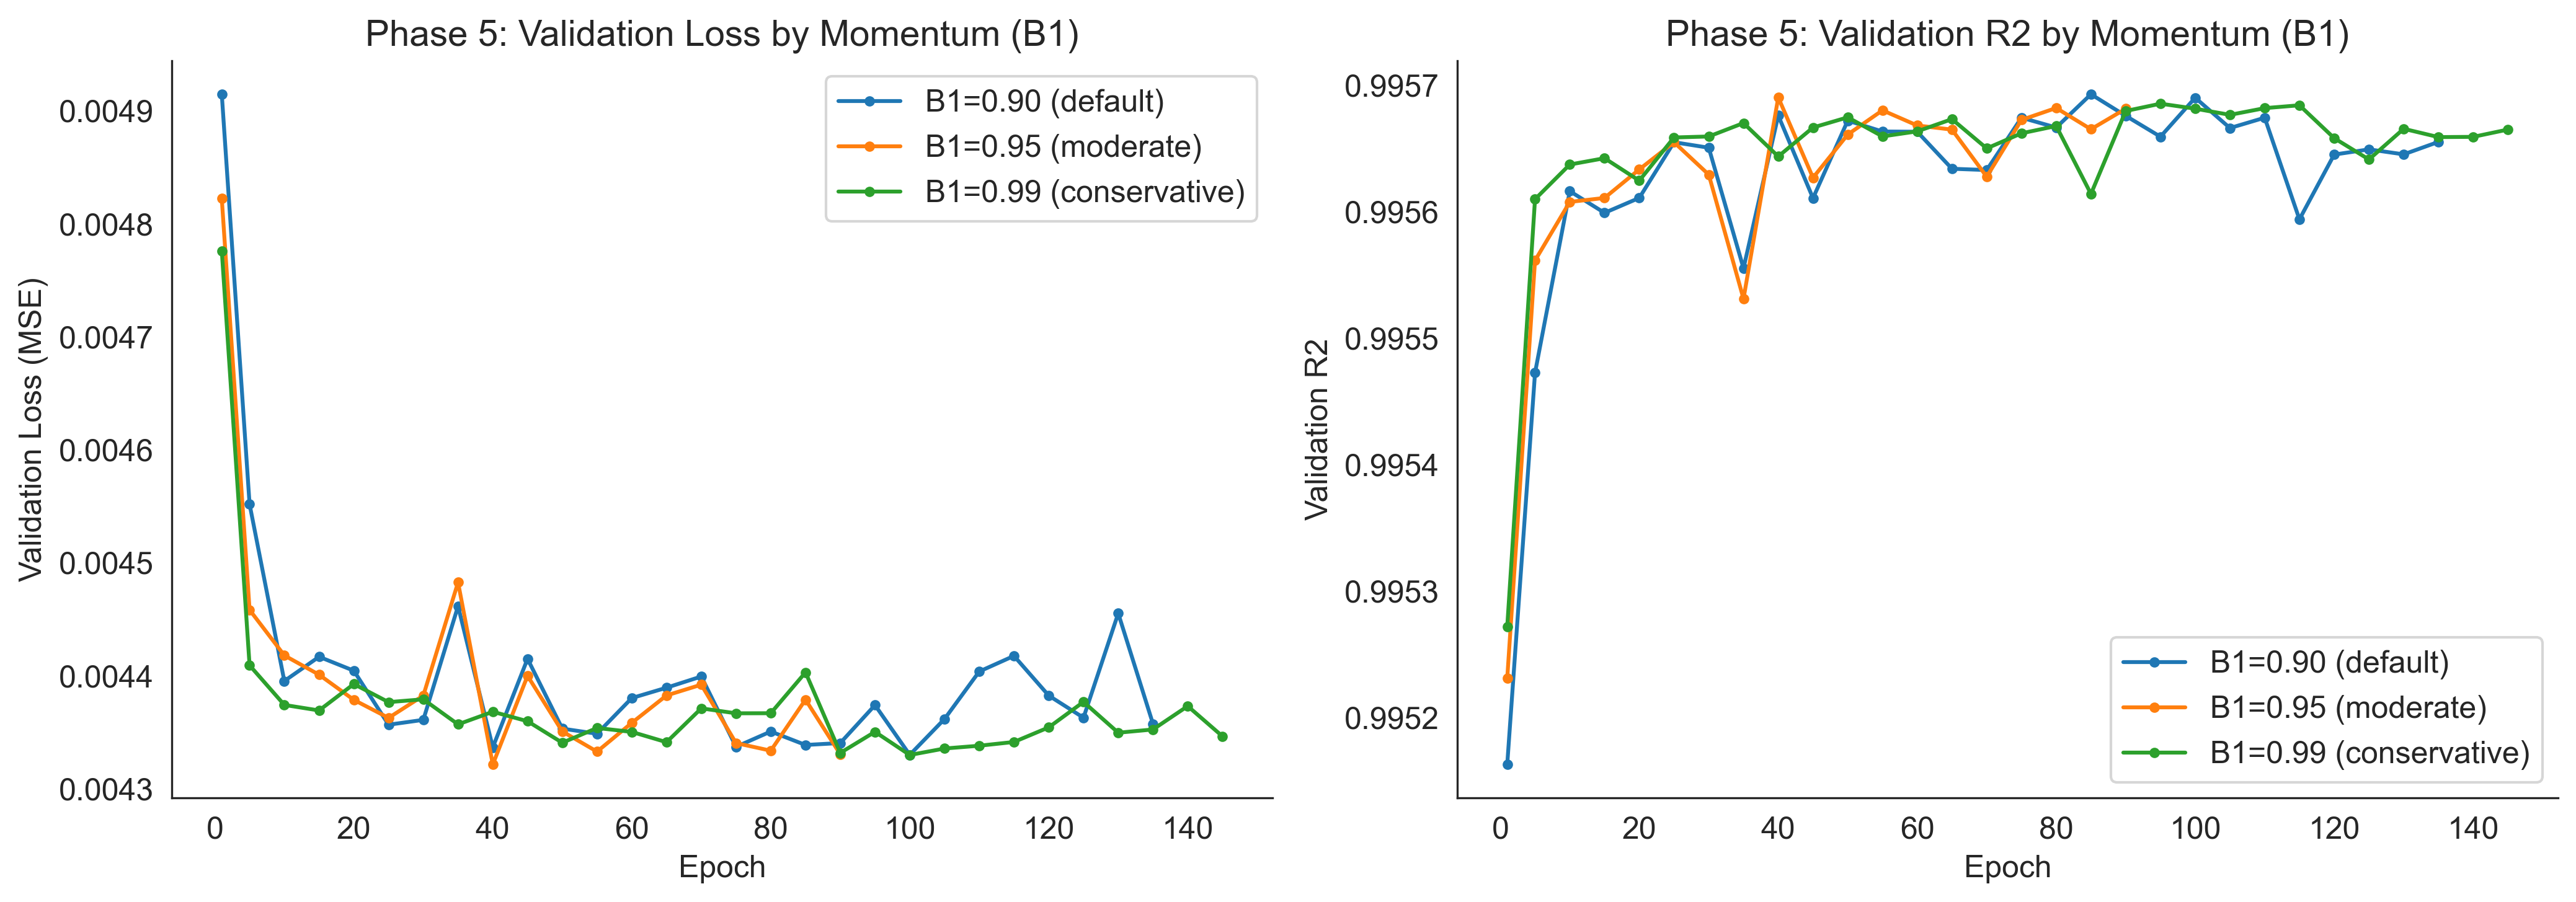
\includegraphics[width=0.95\textwidth]{Thesis/Chapter 4/Figures/fig_phase5_momentum_comparison.png}
\caption{Phase~5: validation MSE loss (left) and validation $R^2$
(right) by first momentum coefficient $\beta_1$.}
\label{fig:phase5_momentum_ch4}
\end{figure}

\noindent
Figure~\ref{fig:phase5_momentum_ch4} shows that all three momentum
configurations converge to similar final validation performance. The
$\beta_1 = 0.95$ configuration achieves marginally lower and more
stable validation loss from epoch~40 onwards, with the best validation
$R^2$ reaching approximately $0.9957$. The conservative setting
$\beta_1 = 0.99$ converges slightly faster in early epochs but exhibits
comparable final performance. The configuration $(\beta_1, \beta_2) =
(0.95, 0.999)$ was retained.

\subsubsection{Hyperparameter comparison overview}

Figure~\ref{fig:validation_loss_overview_ch4} presents the best
validation loss achieved by each configuration across all five phases.

\begin{figure}[H]
\centering
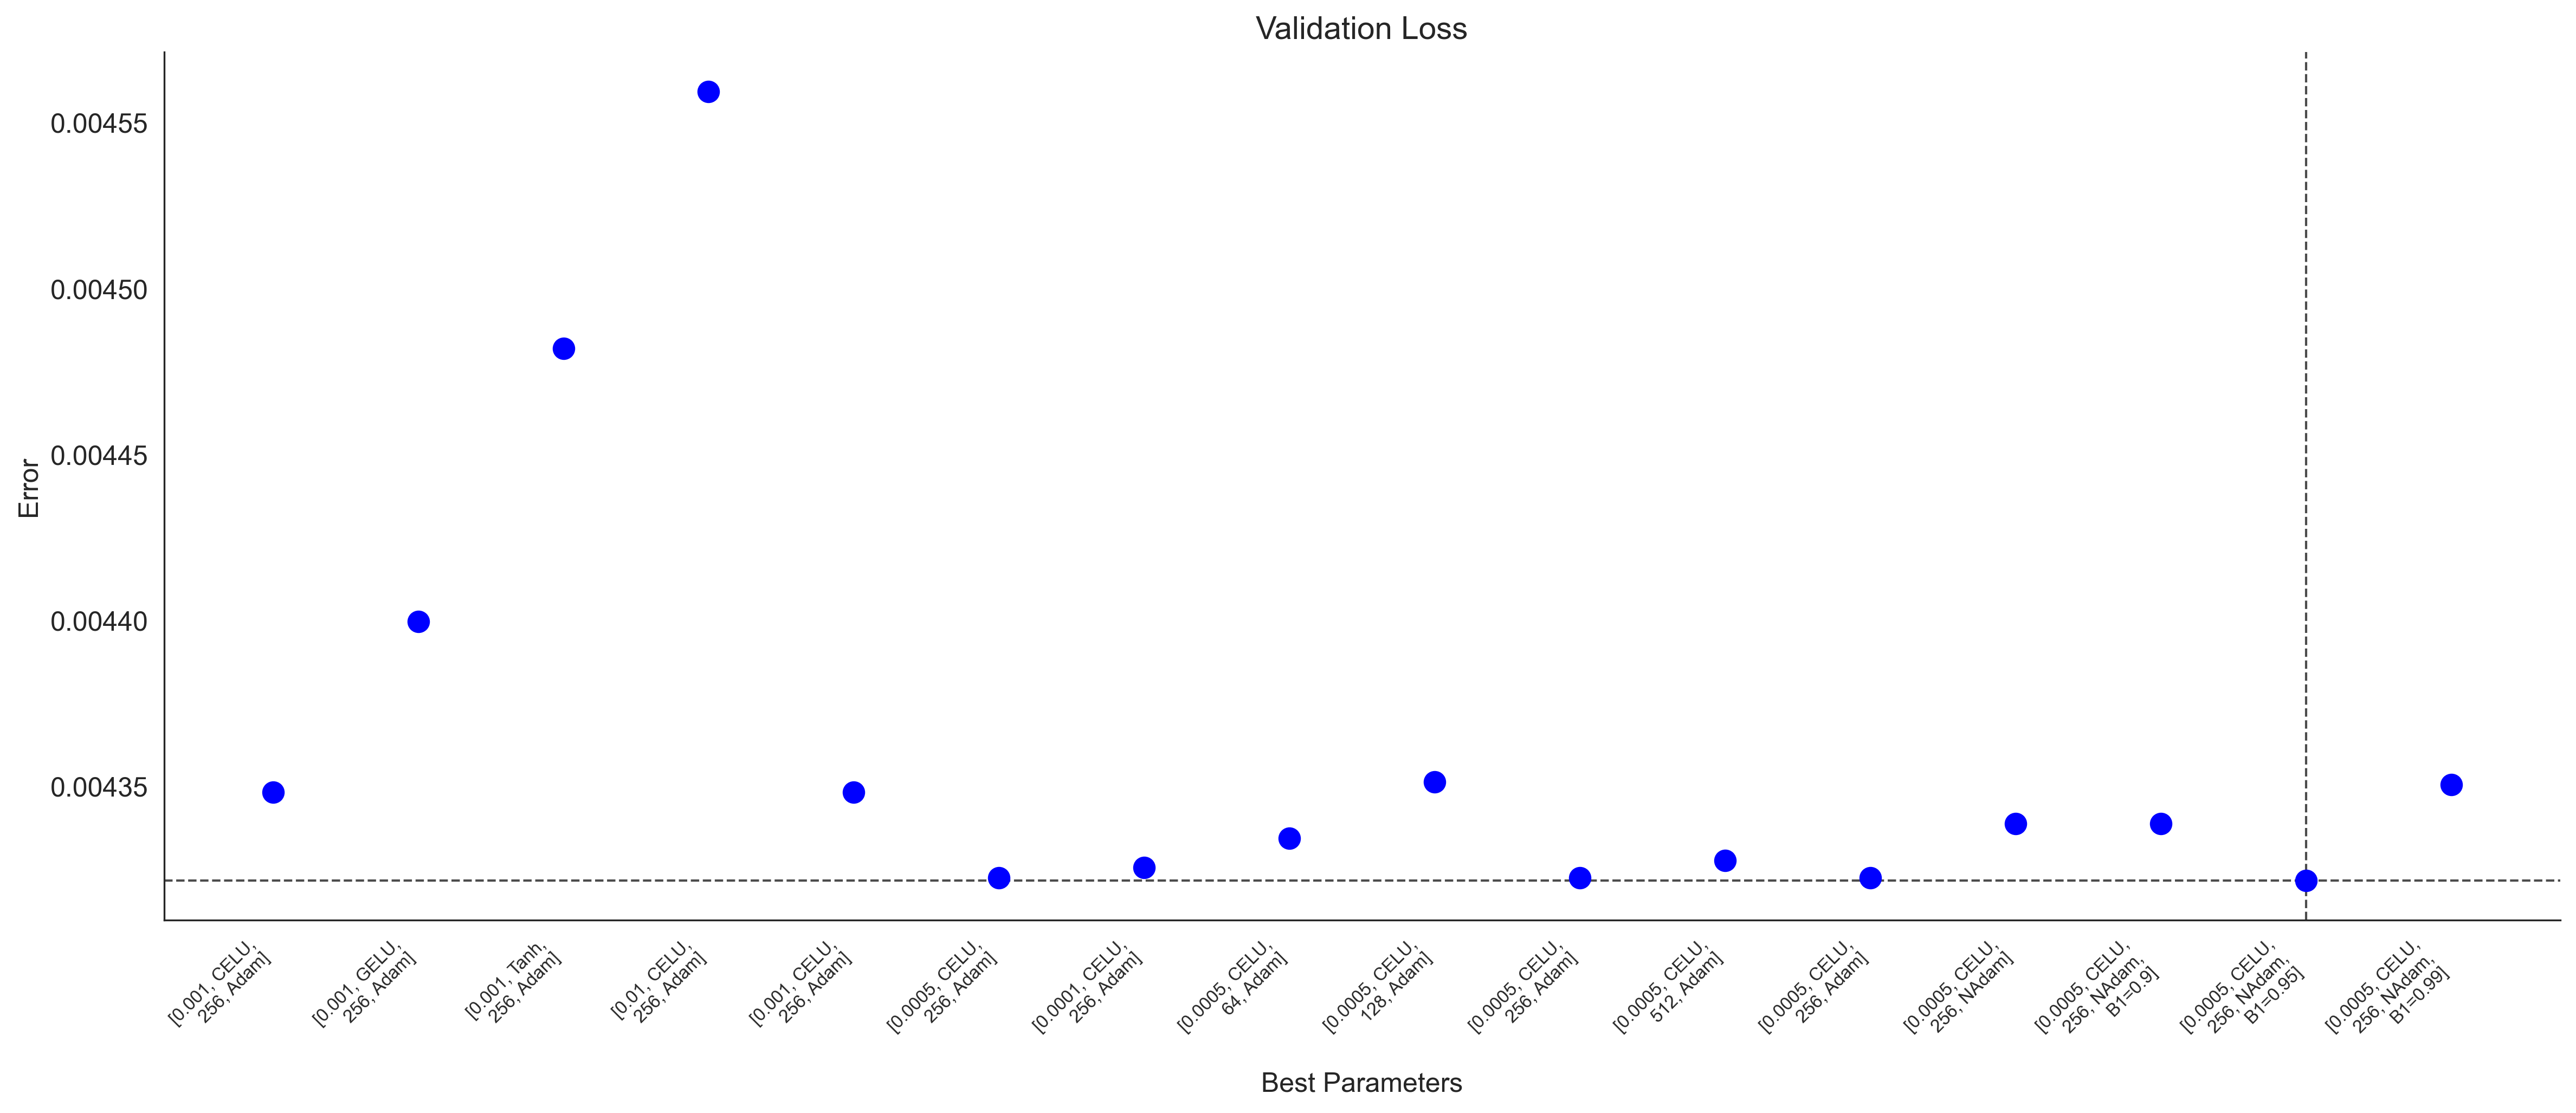
\includegraphics[width=0.95\textwidth]{Thesis/Chapter 4/Figures/fig_validation_loss_hyperparameters.png}
\caption{Best validation MSE loss across all hyperparameter
configurations evaluated in Phases~1-5.}
\label{fig:validation_loss_overview_ch4}
\end{figure}

\noindent
The selected configuration (CELU, $\eta = 0.0005$,
$|\mathcal{B}| = 256$, Nadam, $\beta_1 = 0.95$) achieves the lowest
validation loss among all evaluated configurations.
Table~\ref{tab:final_hyperparameters_ch4} records the final training
configuration.

\begin{table}[H]
\centering
\caption{Selected hyperparameters from the sequential comparison.}
\label{tab:final_hyperparameters_ch4}
\small
\renewcommand{\arraystretch}{1.15}
\begin{tabular}{p{0.30\textwidth}p{0.25\textwidth}p{0.30\textwidth}}
\toprule
\textbf{Phase} & \textbf{Candidates} & \textbf{Selected} \\
\midrule
1. Activation function & CELU, GELU, Tanh & CELU \\
2. Learning rate & 0.01, 0.001, 0.0005, 0.0001 & 0.0005 \\
3. Batch size & 64, 128, 256, 512 & 256 \\
4. Optimiser & Adam, Nadam & Nadam \\
5. Momentum $(\beta_1, \beta_2)$ & (0.90, 0.999), (0.95, 0.999), (0.99, 0.999) & (0.95, 0.999) \\
\bottomrule
\end{tabular}
\end{table}

\subsubsection{Final model predictive performance}

The final \gls{dnn} was retrained with the selected configuration and
early stopping at epoch $e^{*} = 85$ (the checkpoint with the highest
validation $R^2$).
Table~\ref{tab:final_model_performance_ch4} reports the predictive
performance metrics computed on the original monetary scale after
de-normalising the fitted predictions, using the \gls{mae}
(equation~\eqref{eq:mae}), \gls{rmse} (equation~\eqref{eq:rmse}), and
$R^2$ (equation~\eqref{eq:r_squared}).

\begin{table}[H]
\centering
\caption{Predictive performance of the final DNN on the original
monetary scale.}
\label{tab:final_model_performance_ch4}
\small
\renewcommand{\arraystretch}{1.15}
\begin{tabular}{lrrr}
\toprule
\textbf{Partition} & \textbf{MAE (R)} & \textbf{RMSE (R)} & $\boldsymbol{R^2}$ \\
\midrule
Training ($n = 524\,288$) & 251 & 291 & 0.9957 \\
Test ($n = 237\,856$) & 251 & 290 & 0.9957 \\
\bottomrule
\end{tabular}
\end{table}

\noindent
The near-identical performance across partitions (MAE = R251 on both;
RMSE within R290 to R291; $R^2 = 0.9957$ on both) confirms that the
fitted model generalises to unseen data without overfitting.  The
training-set response statistics used for standardisation are
$\overline{y}_{\mathrm{train}} = \text{R16\,744}$ and
$s_{y,\mathrm{train}} = \text{R4\,419}$.  On the standardised scale,
the validation MSE at the selected epoch $e^{*} = 85$ is $0.00432$
(Figure~\ref{fig:validation_loss_overview_ch4}), and the
original-scale residuals range from approximately $-600$ to $+600$ as
characterised in the residual diagnostics of
Section~\ref{sec:model_validation_diagnostics}.

The model's predictive performance supports its use in the
subsequent simulation and attribution analyses.

\subsubsection{Baseline comparison: GLM (Gamma, log-link) versus DNN}
\label{sec:glm_vs_dnn_comparison_ch4}

The \gls{glm} benchmark specified in
Section~\ref{sec:glm_benchmark_methods} was evaluated alongside the
\gls{dnn}.  Table~\ref{tab:glm_vs_dnn_comparison_ch4} reports the
performance of both models across training, validation and test
partitions.

\begin{table}[H]
\centering
\caption{Predictive performance comparison: \gls{glm} (Gamma, log-link)
versus \gls{dnn} (funnel architecture) on the original monetary scale.}
\label{tab:glm_vs_dnn_comparison_ch4}
\small
\renewcommand{\arraystretch}{1.15}
\begin{tabular}{llrrr}
\toprule
\textbf{Model} & \textbf{Partition} & \textbf{MAE (R)} &
\textbf{RMSE (R)} & $\boldsymbol{R^2}$ \\
\midrule
\gls{glm} (Gamma, log-link)
    & Training   & 623 & 911 & 0.9574 \\
    & Validation & 622 & 913 & 0.9574 \\
    & Test       & 624 & 913 & 0.9571 \\
\addlinespace
\gls{dnn} (Funnel)
    & Training   & 251 & 291 & 0.9957 \\
    & Validation & 251 & 291 & 0.9957 \\
    & Test       & 251 & 290 & 0.9957 \\
\bottomrule
\end{tabular}
\end{table}

\noindent
The \gls{dnn} outperforms the \gls{glm} on every metric.  On the test
set, the \gls{dnn} achieves an $R^2$ of $0.9957$ compared with
$0.9571$ for the \gls{glm}, an improvement of $3.86$ percentage points.
The test \gls{rmse} decreases from R913 to R290 (a $68.2\%$ reduction),
and the test \gls{mae} decreases from R624 to R251 (a $59.8\%$
reduction).

\begin{figure}[H]
\centering
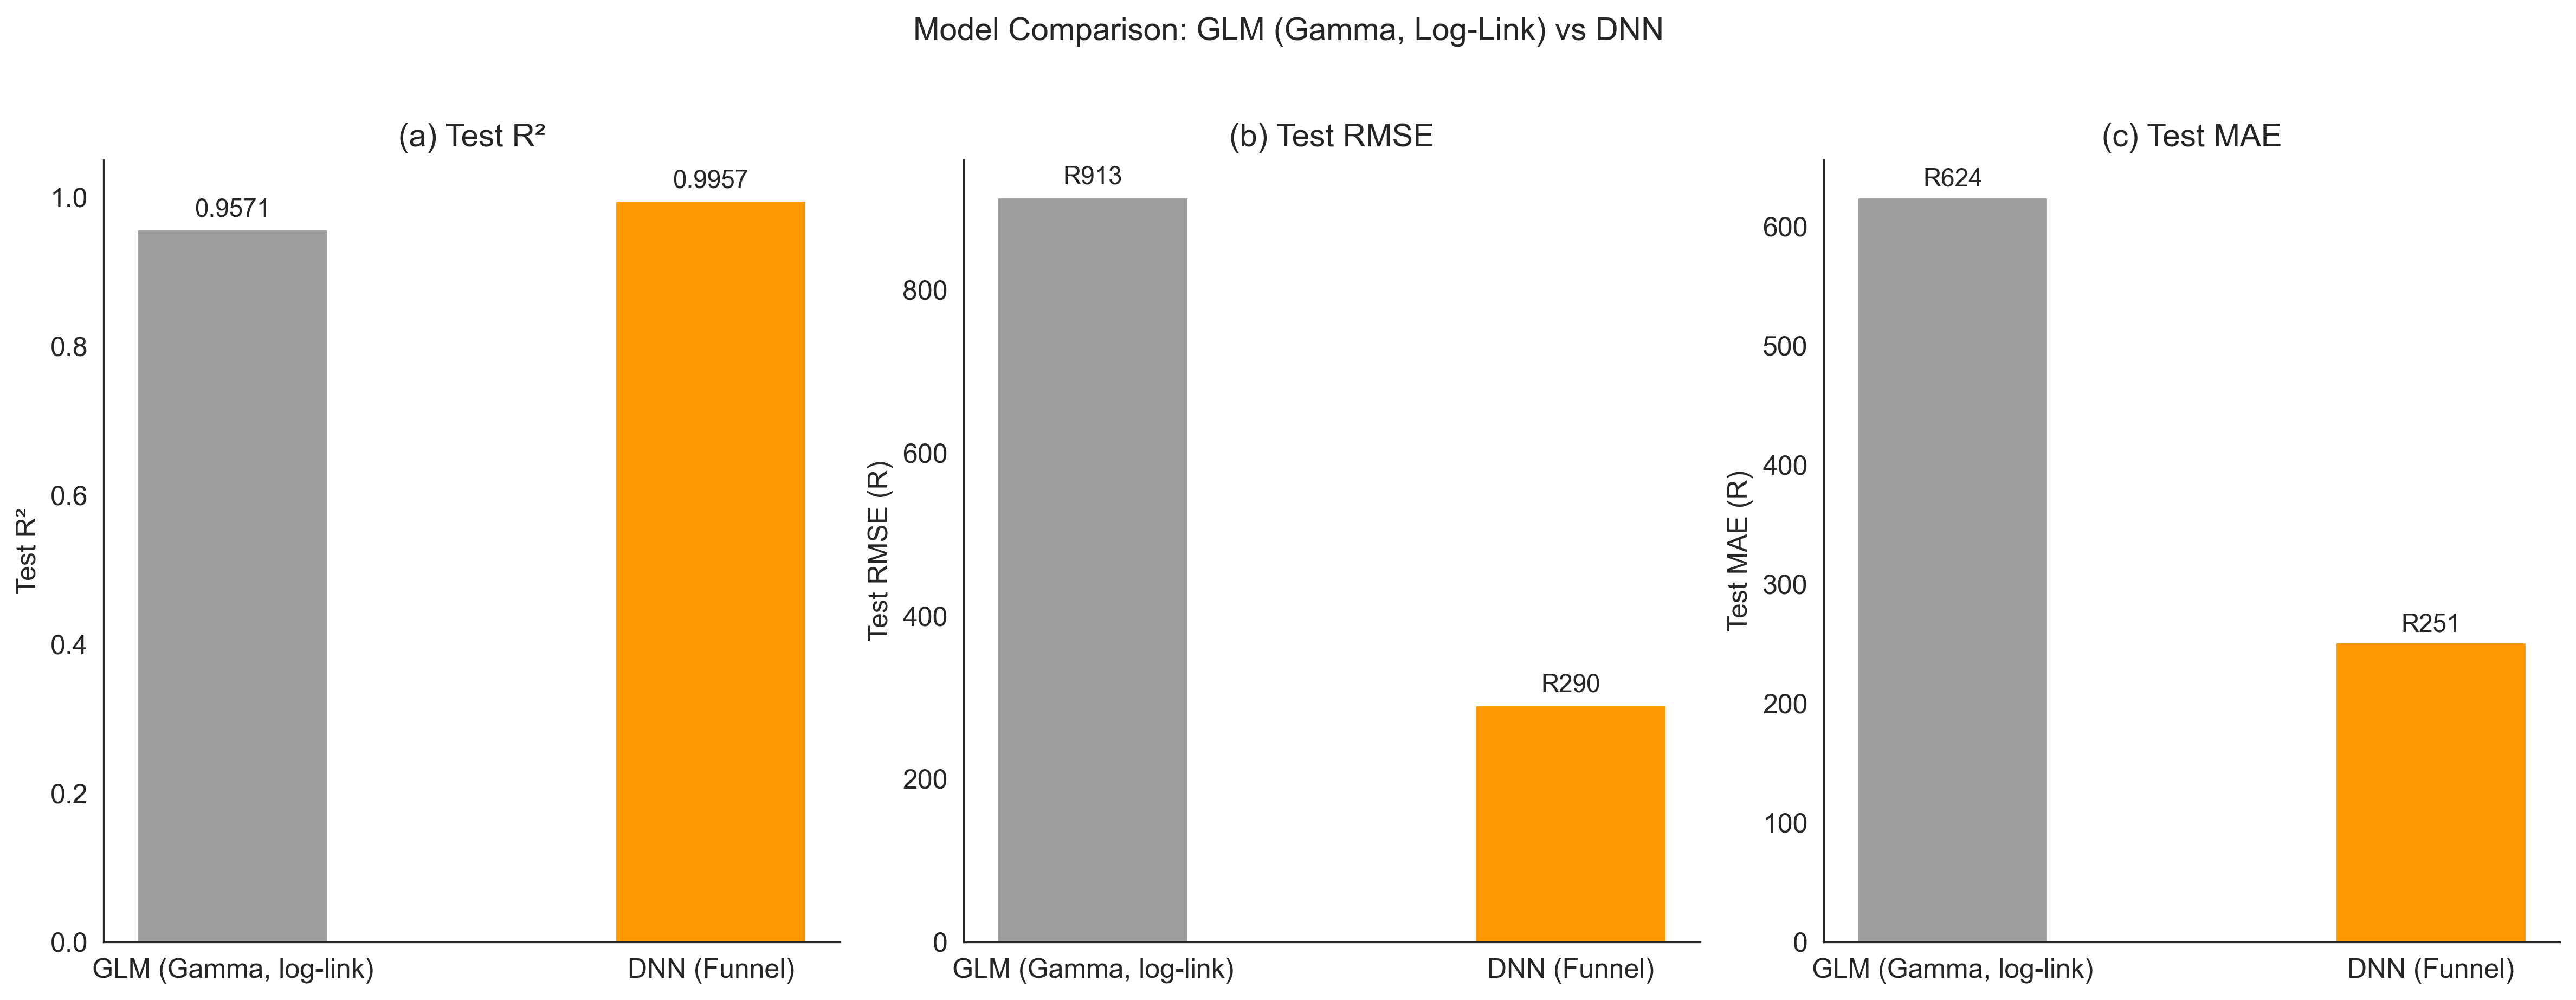
\includegraphics[width=0.95\textwidth]{Thesis/Chapter 4/Figures/fig_glm_vs_dnn_comparison.png}
\caption{Test-set performance comparison: \gls{glm} (Gamma, log-link)
versus \gls{dnn}.  (a)~Test $R^2$; (b)~test RMSE; (c)~test MAE.}
\label{fig:glm_vs_dnn_comparison_ch4}
\end{figure}

\noindent
Figure~\ref{fig:glm_vs_dnn_comparison_ch4} visualises the test-set
comparison.  The \gls{glm}'s inferior fit is attributable to the
log-link's multiplicative mean structure, which does not match the
additive data-generating process underlying this dataset.  The charges
variable is constructed as an approximately linear function of the input
features plus noise; the \gls{glm}'s exponential inverse-link therefore
introduces systematic model misspecification.  The \gls{dnn}, by
contrast, learns the additive structure directly through its flexible
hidden-layer representations.

\begin{figure}[H]
\centering
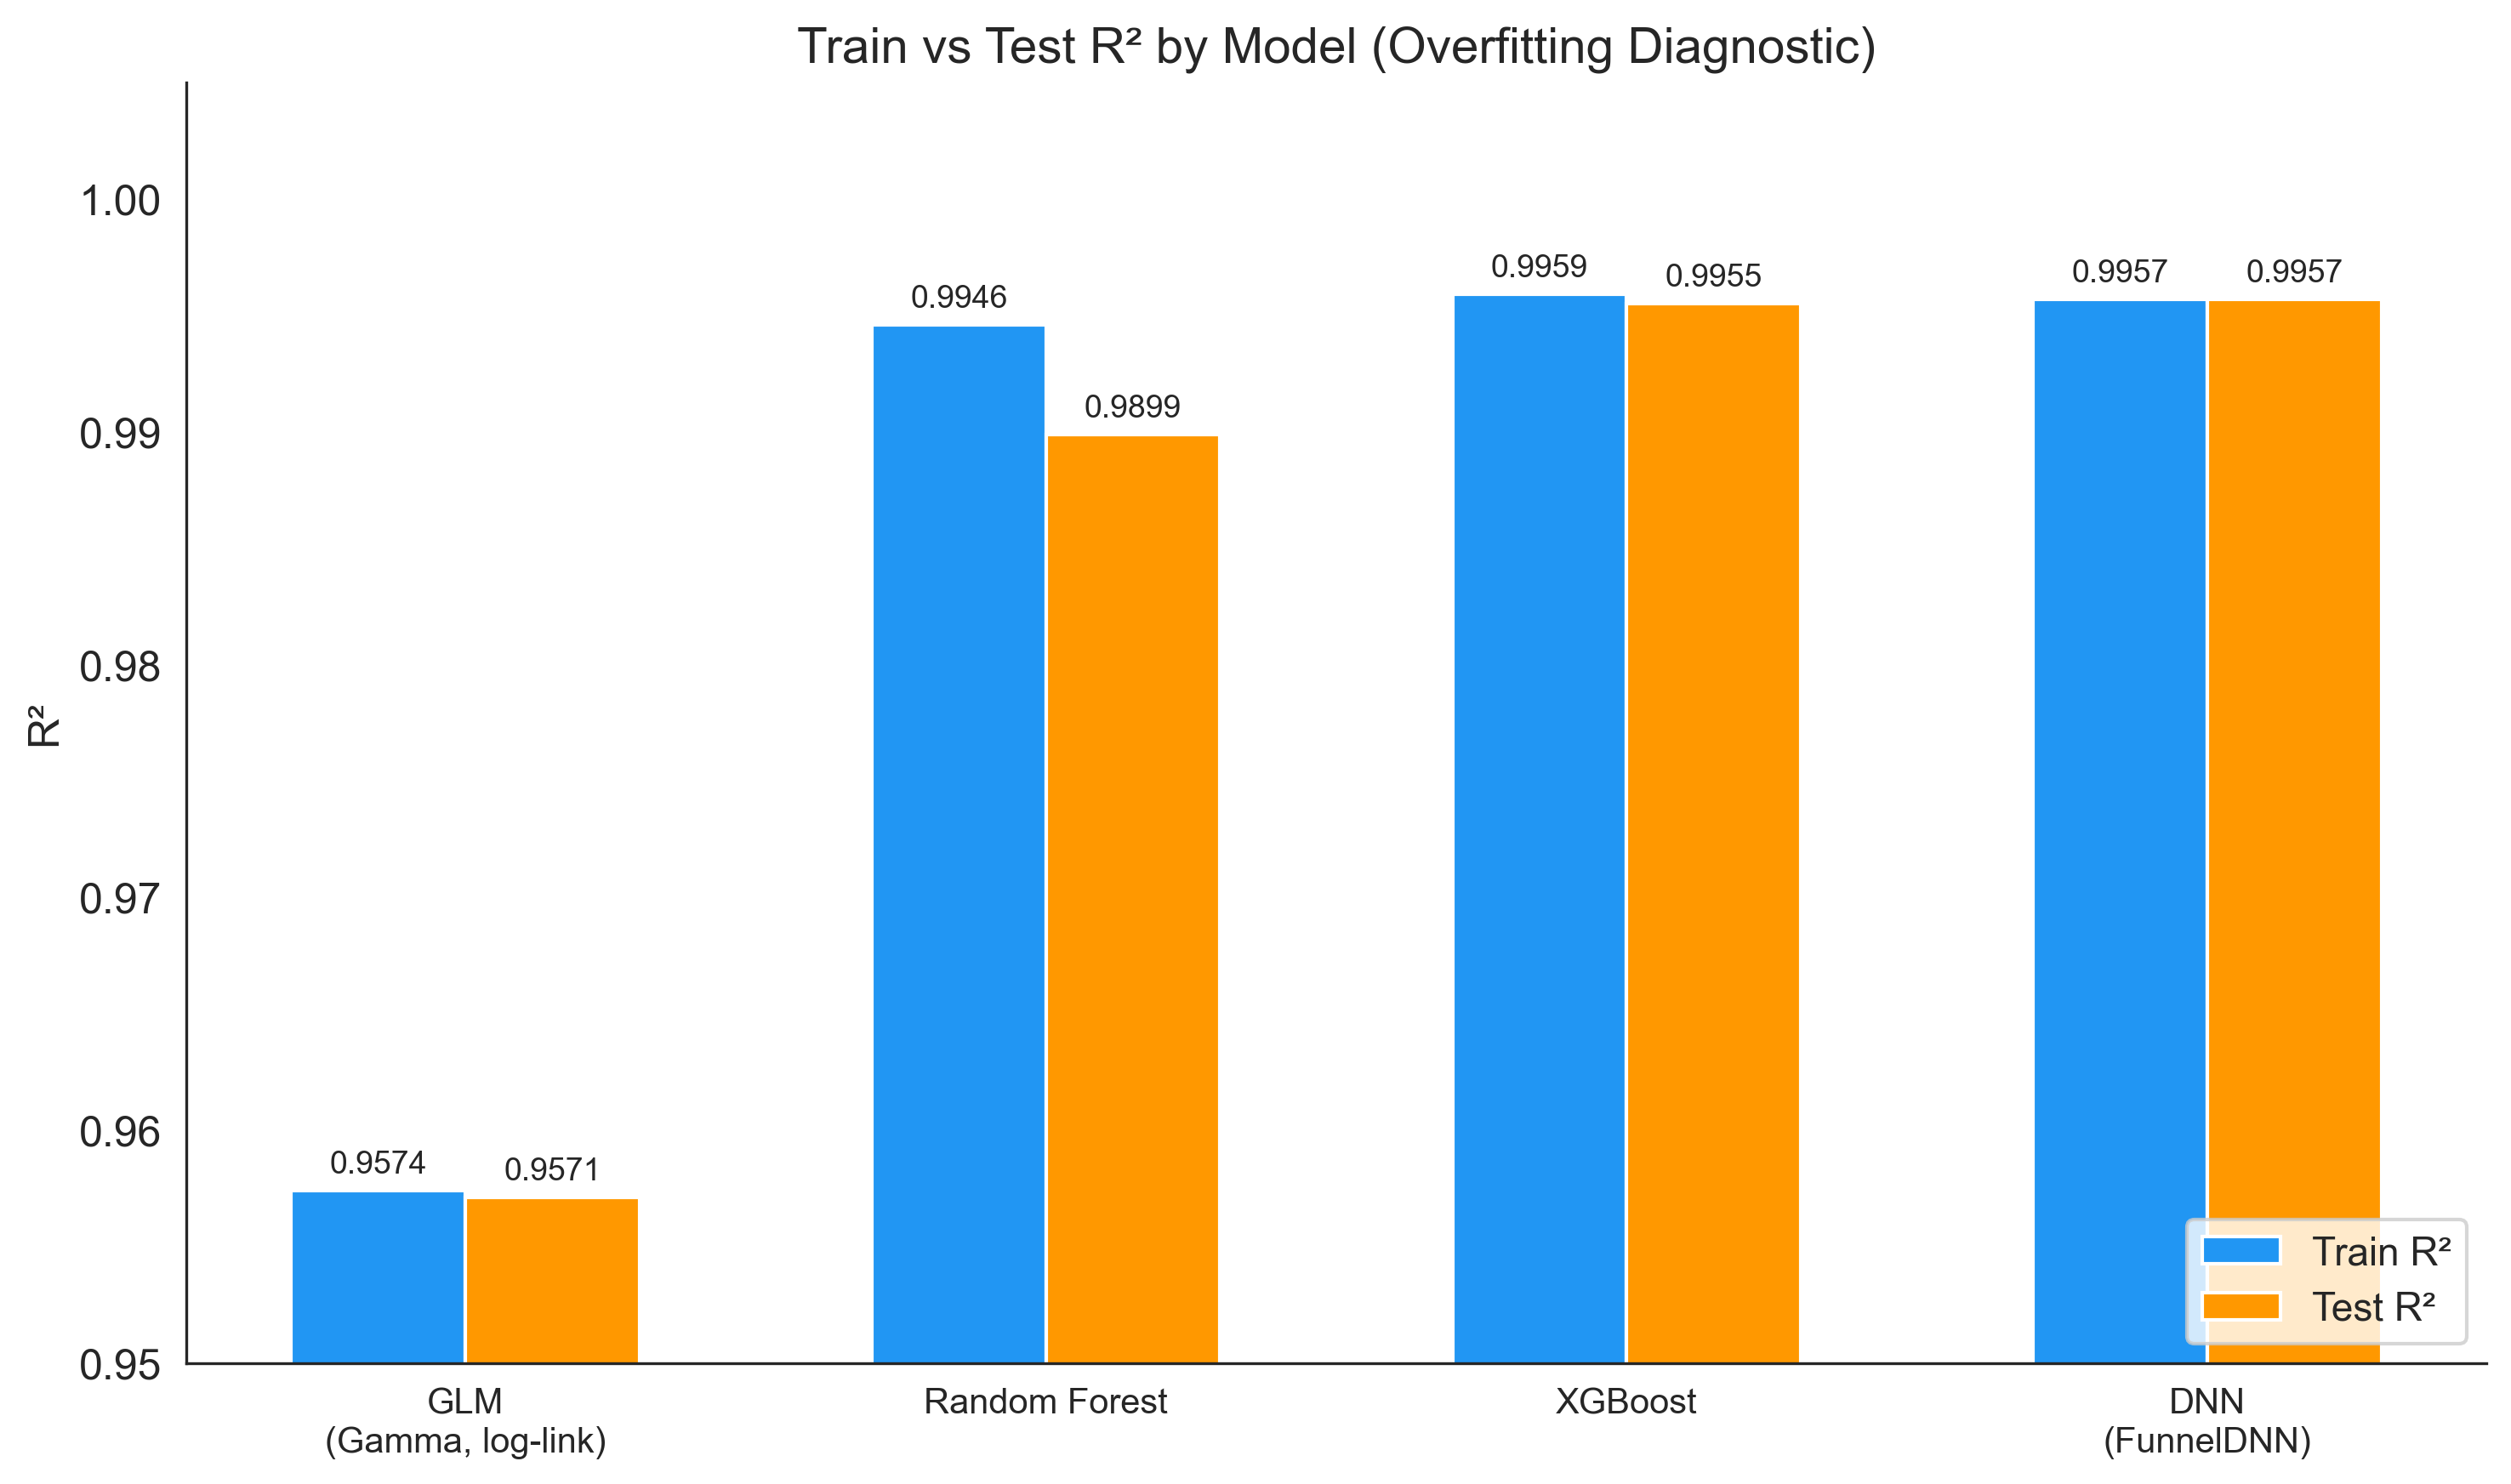
\includegraphics[width=0.65\textwidth]{Thesis/Chapter 4/Figures/fig_train_test_r2_overfitting.png}
\caption{Overfitting diagnostic: training versus test $R^2$ for both
models.}
\label{fig:train_test_r2_overfitting_ch4}
\end{figure}

\noindent
Figure~\ref{fig:train_test_r2_overfitting_ch4} compares the training
and test $R^2$ for both models.  The \gls{glm} shows negligible
generalisation loss ($R^2_{\mathrm{train}} = 0.9574$ versus
$R^2_{\mathrm{test}} = 0.9571$), as expected for a parametric model
with far fewer parameters than observations.  The \gls{dnn} likewise
shows no evidence of overfitting ($R^2_{\mathrm{train}} = 0.9957$
versus $R^2_{\mathrm{test}} = 0.9957$), confirming that the early
stopping criterion (Section~\ref{sec:dnn_specification_training})
effectively regularises the 49\,168 trainable parameters.

The \gls{glm} comparison serves two purposes.  First, it establishes
that the \gls{dnn}'s high $R^2$ reflects genuine predictive superiority
over the actuarial-standard model class, not merely an artefact of the
dataset's synthetic regularity.  Second, because the Gamma/log-link
\gls{glm} is the model an actuary would deploy as a first approach, the
comparison provides the practical benchmark context that situates the
\gls{dnn} within the actuarial modelling landscape.  The \gls{dnn} is therefore retained for the subsequent analyses
on the grounds of its superior accuracy and its differentiability
for gradient-based attribution.

The finding that a deep neural network outperforms a classical \gls{glm}
on this benchmark is consistent with the broader health-cost prediction
literature.  \citet{dreweboss2022deep} report that deep-learning models
achieve lower prediction error than standard actuarial models on claims
data, while \citet{samiuddin2023health} and \citet{kaushik2022machine}
similarly observe that neural-network architectures improve upon
traditional regression baselines for insurance cost estimation.  As noted
in Section~\ref{sec:integrating_dnn_mc_shapley}, however, this
superiority is not universal across all tabular insurance datasets
\citep{richman2021ai}, and the present comparison is limited to a single
classical baseline on a benchmark dataset with a strong synthetic
structure.


% =============================================================
\subsection{Monte Carlo Predicted-Cost Distribution}
\label{sec:mc_results}

The base parametric Monte Carlo simulation (Algorithm~3.1) was executed
with $B = 10\,000$ synthetic policyholder profiles drawn from the
product-marginal input distribution specified in
equation~\eqref{eq:raw_product_mc_distribution_ch3}. Each simulated
profile was preprocessed, scored through the fitted \gls{dnn}, and
de-normalised to the original monetary scale.

\subsubsection{Simulated input validation}
\label{sec:simulated_input_validation_ch4}

The simulated inputs were validated following the joint-distribution
diagnostic protocol in Section~\ref{sec:mc_input_validation}.

\subsubsection*{Joint distribution validation}

Three complementary diagnostics compare the bivariate and multivariate
dependence structure of the training data with that of the Monte Carlo
sample.

\begin{figure}[H]
\centering
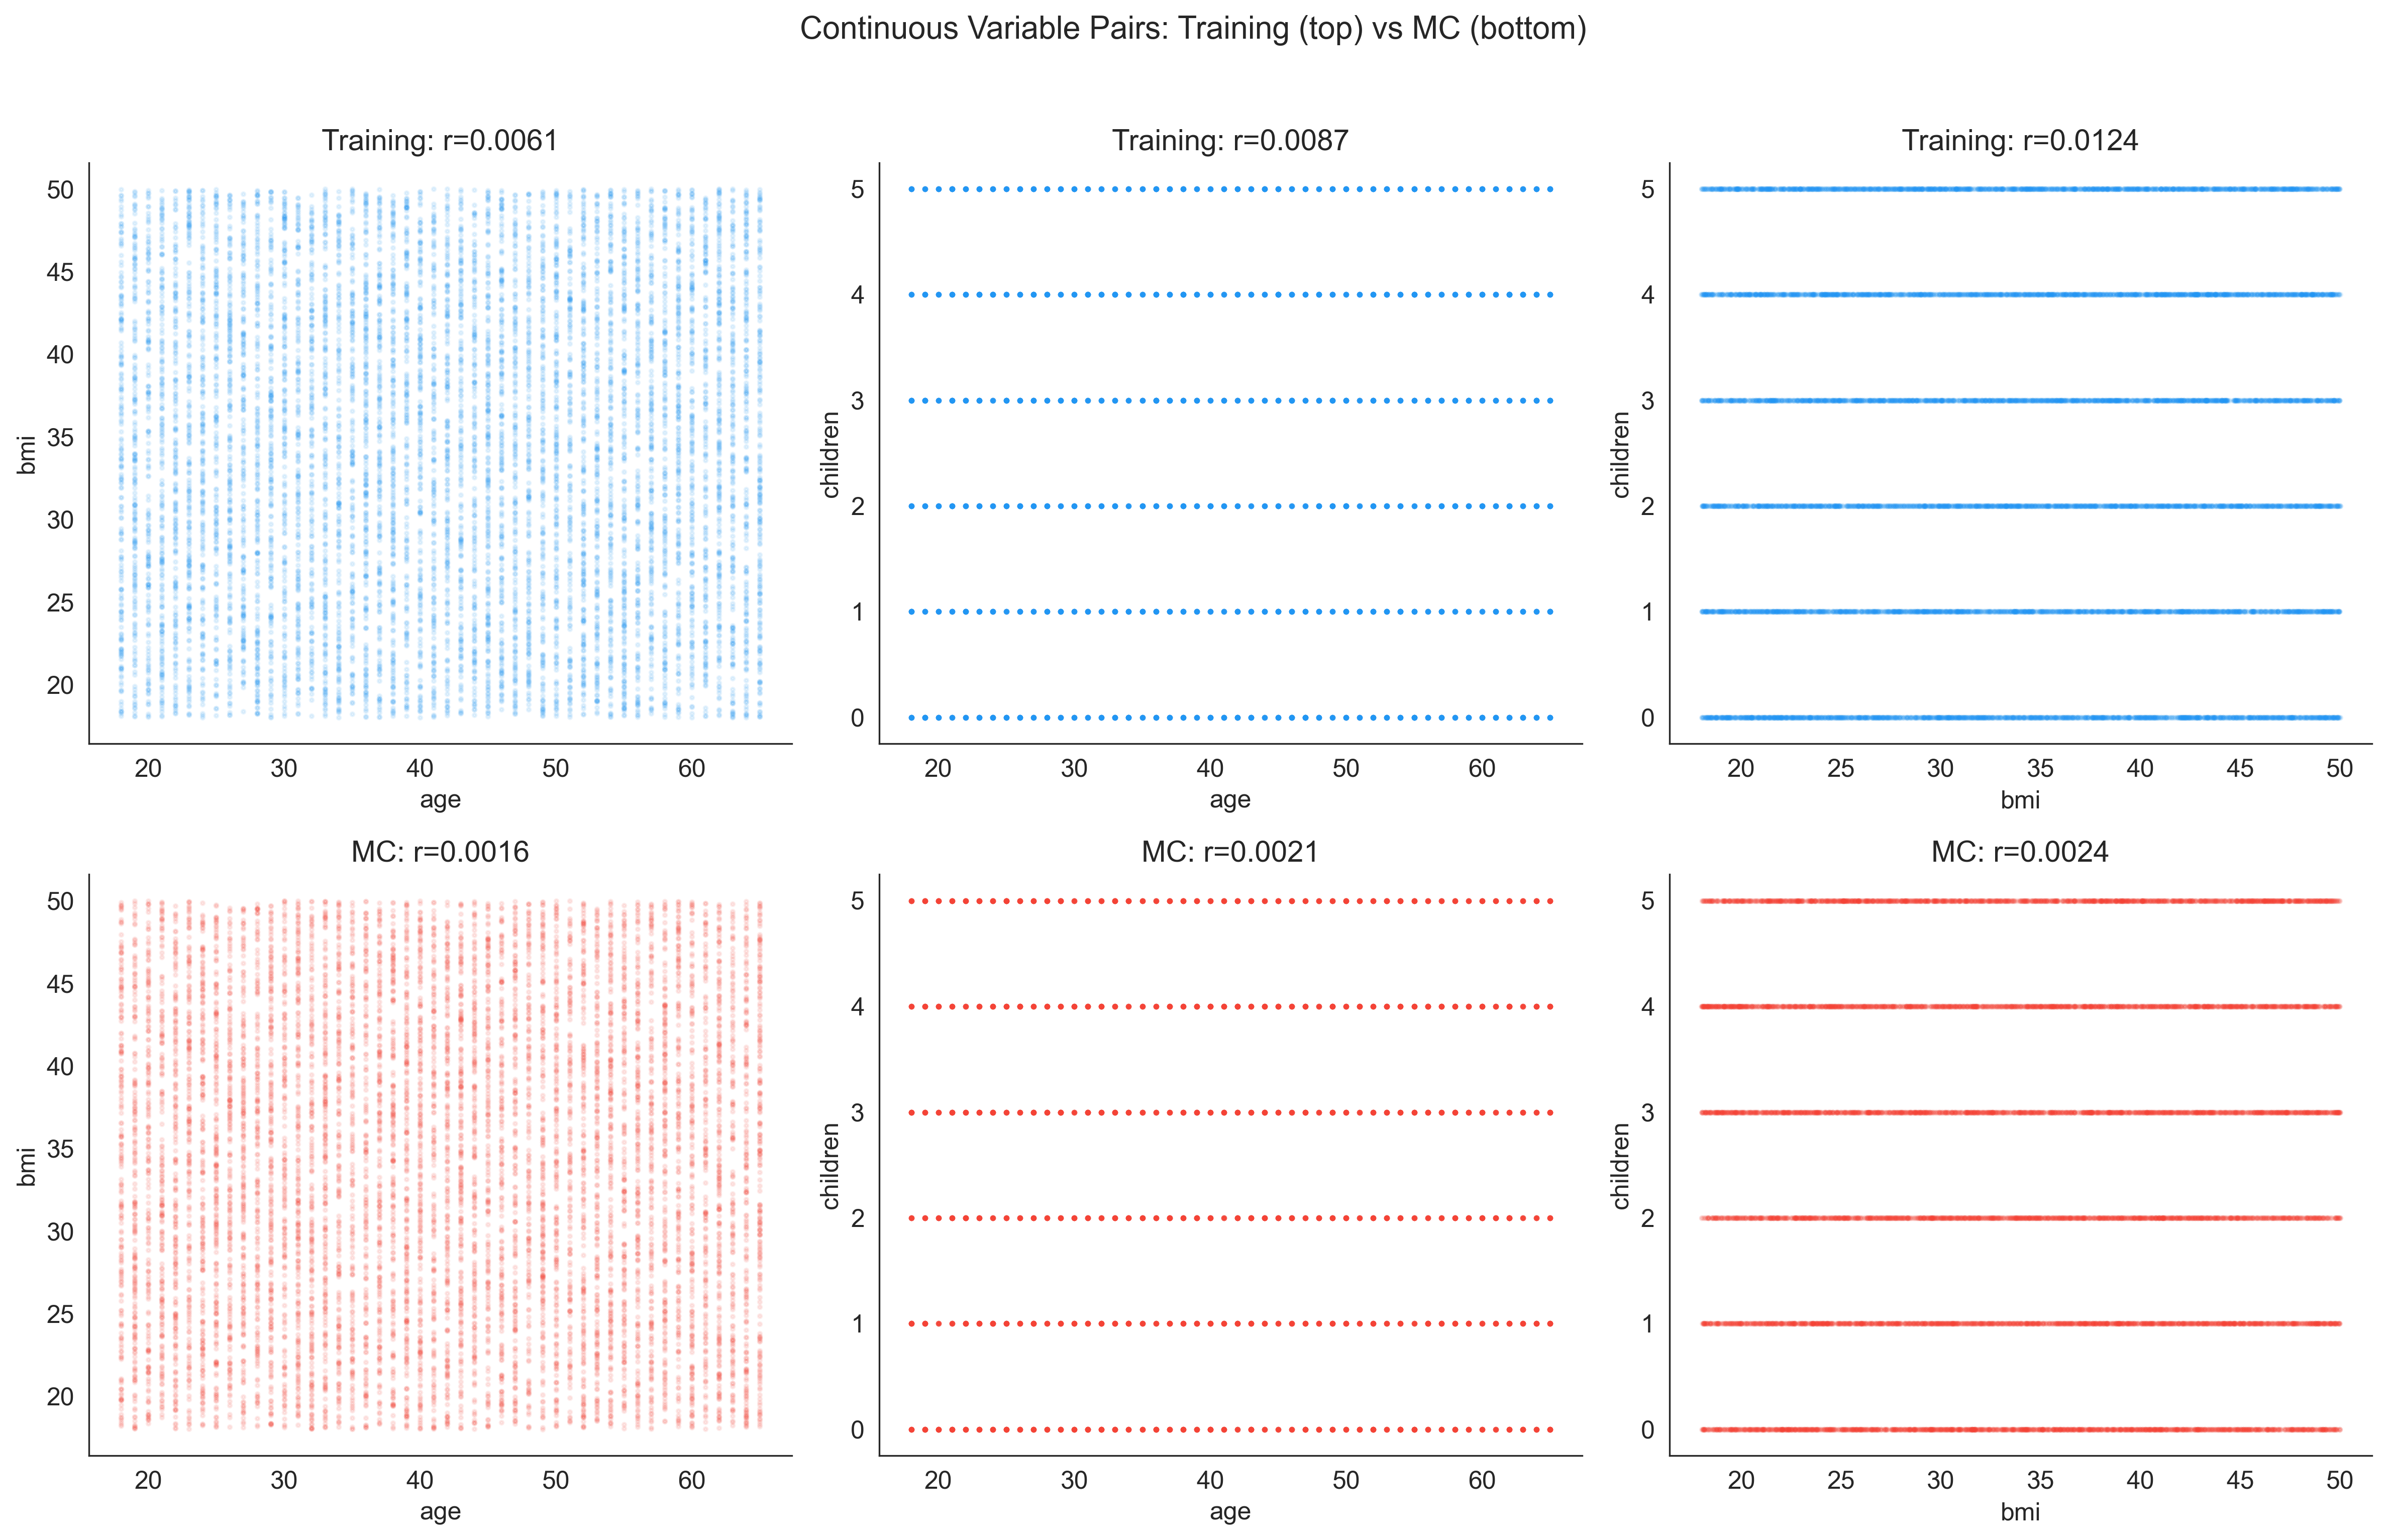
\includegraphics[width=0.95\textwidth]{Thesis/Chapter 4/Figures/fig_mc_joint_continuous_pairs.png}
\caption{Continuous variable pairs: training (top row, blue) versus
Monte Carlo (bottom row, red).}
\label{fig:mc_joint_continuous_pairs_ch4}
\end{figure}

\noindent
Figure~\ref{fig:mc_joint_continuous_pairs_ch4} displays pairwise
scatter plots for the three continuous variables (\texttt{age},
\texttt{bmi}, \texttt{children}).  In the training data, all pairwise
Pearson correlations are negligible ($r = 0.006$, $0.009$, $0.012$).
The Monte Carlo sample shows even weaker correlations ($r = 0.002$,
$0.002$, $0.002$), as expected under independence.  The near-zero
training correlations confirm that the product-marginal simulation does
not discard meaningful continuous dependence.

\begin{figure}[H]
\centering
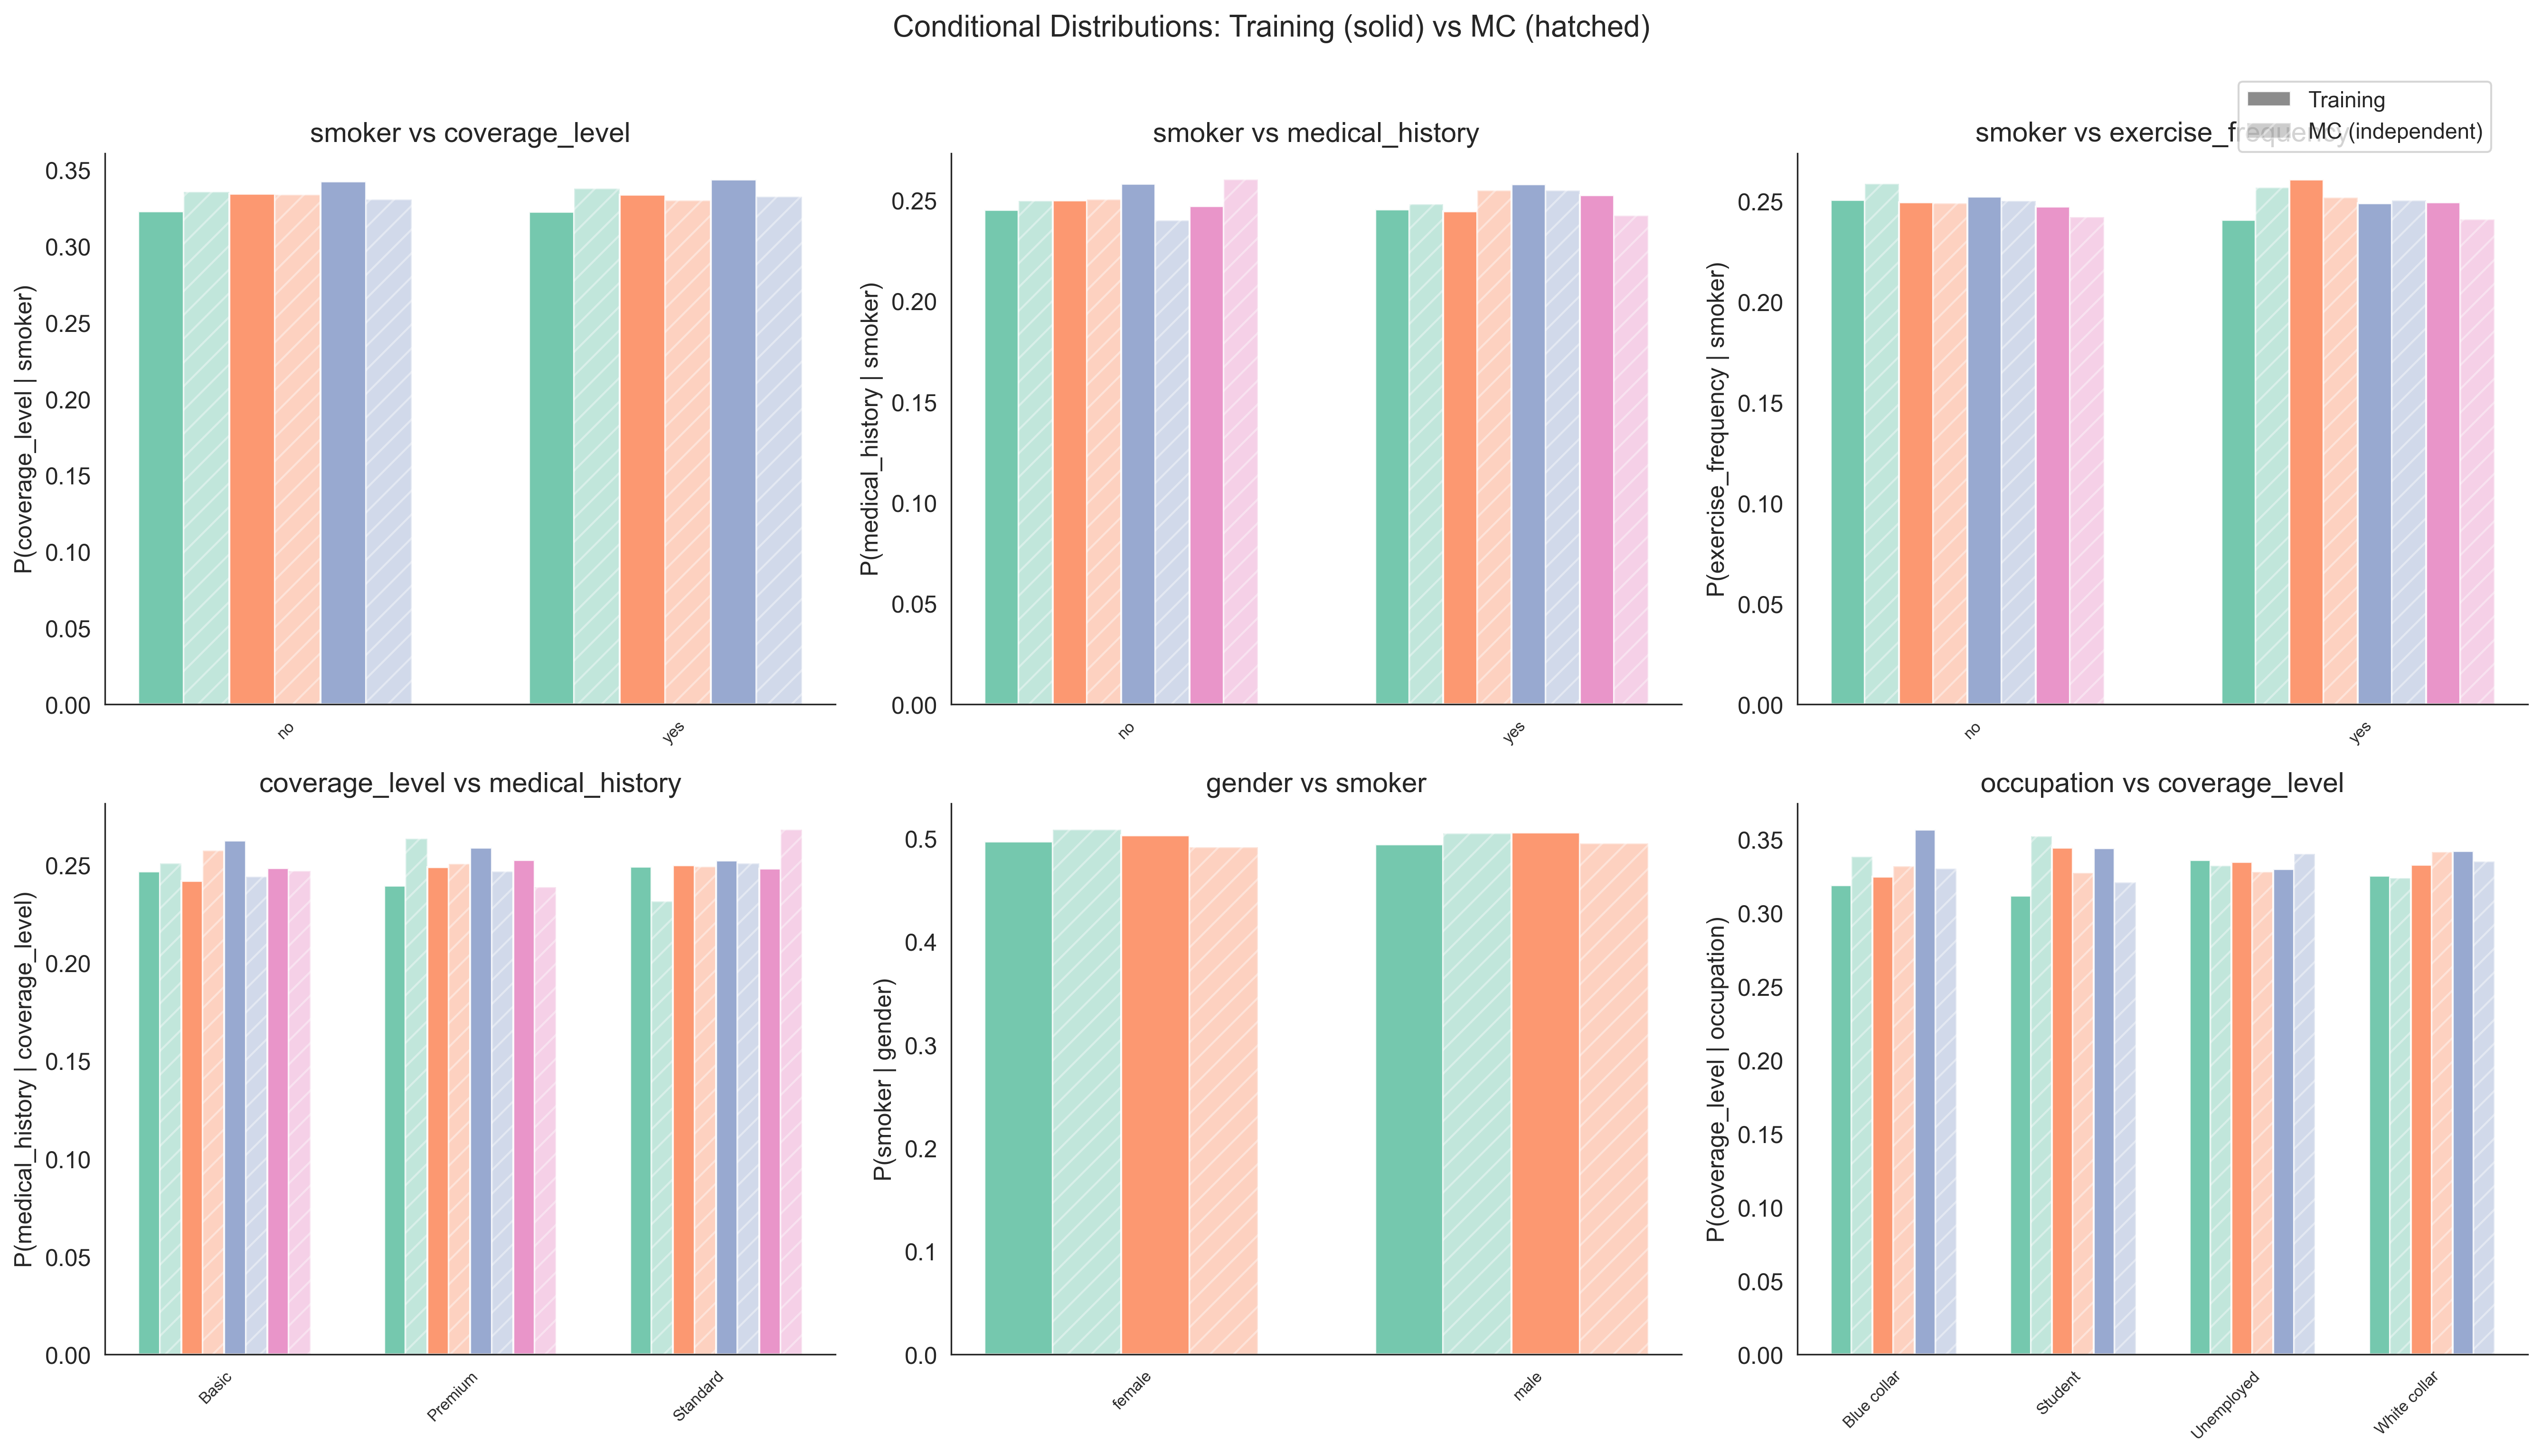
\includegraphics[width=0.95\textwidth]{Thesis/Chapter 4/Figures/fig_mc_joint_crosstabs.png}
\caption{Conditional distributions of selected categorical variable
pairs: training (solid bars) versus Monte Carlo (hatched bars).}
\label{fig:mc_joint_crosstabs_ch4}
\end{figure}

\noindent
Figure~\ref{fig:mc_joint_crosstabs_ch4} compares the conditional
distributions of six key categorical variable pairs.  In each panel,
the conditional proportions are approximately uniform across the
categories of the conditioning variable, both in the training data and
in the Monte Carlo sample.  For instance, the distribution of
\texttt{coverage\_level} given \texttt{smoker} is near-uniform in both
regimes, and the distribution of \texttt{medical\_history} given
\texttt{smoker} is similarly uniform.  These cross-tabulations indicate
that the training-data categoricals are effectively independent of one
another, and the product-marginal simulation preserves this structure.

These bivariate diagnostics complement the correlation-matrix and
Cram\'{e}r's~$V$ comparisons reported in
Section~\ref{sec:mc_input_validation}, which showed that the Pearson
correlation structure and categorical association structure of the
training data are closely reproduced by the parametric Monte Carlo
sample.

\subsubsection*{Higher-order interaction check}

To confirm that the negligible dependence extends beyond pairwise
associations, three-way joint proportions were computed for the four
categorical variables most relevant to the high-cost analysis
(\texttt{smoker}, \texttt{coverage\_level}, \texttt{medical\_history},
\texttt{family\_medical\_history}).

\begin{figure}[H]
\centering
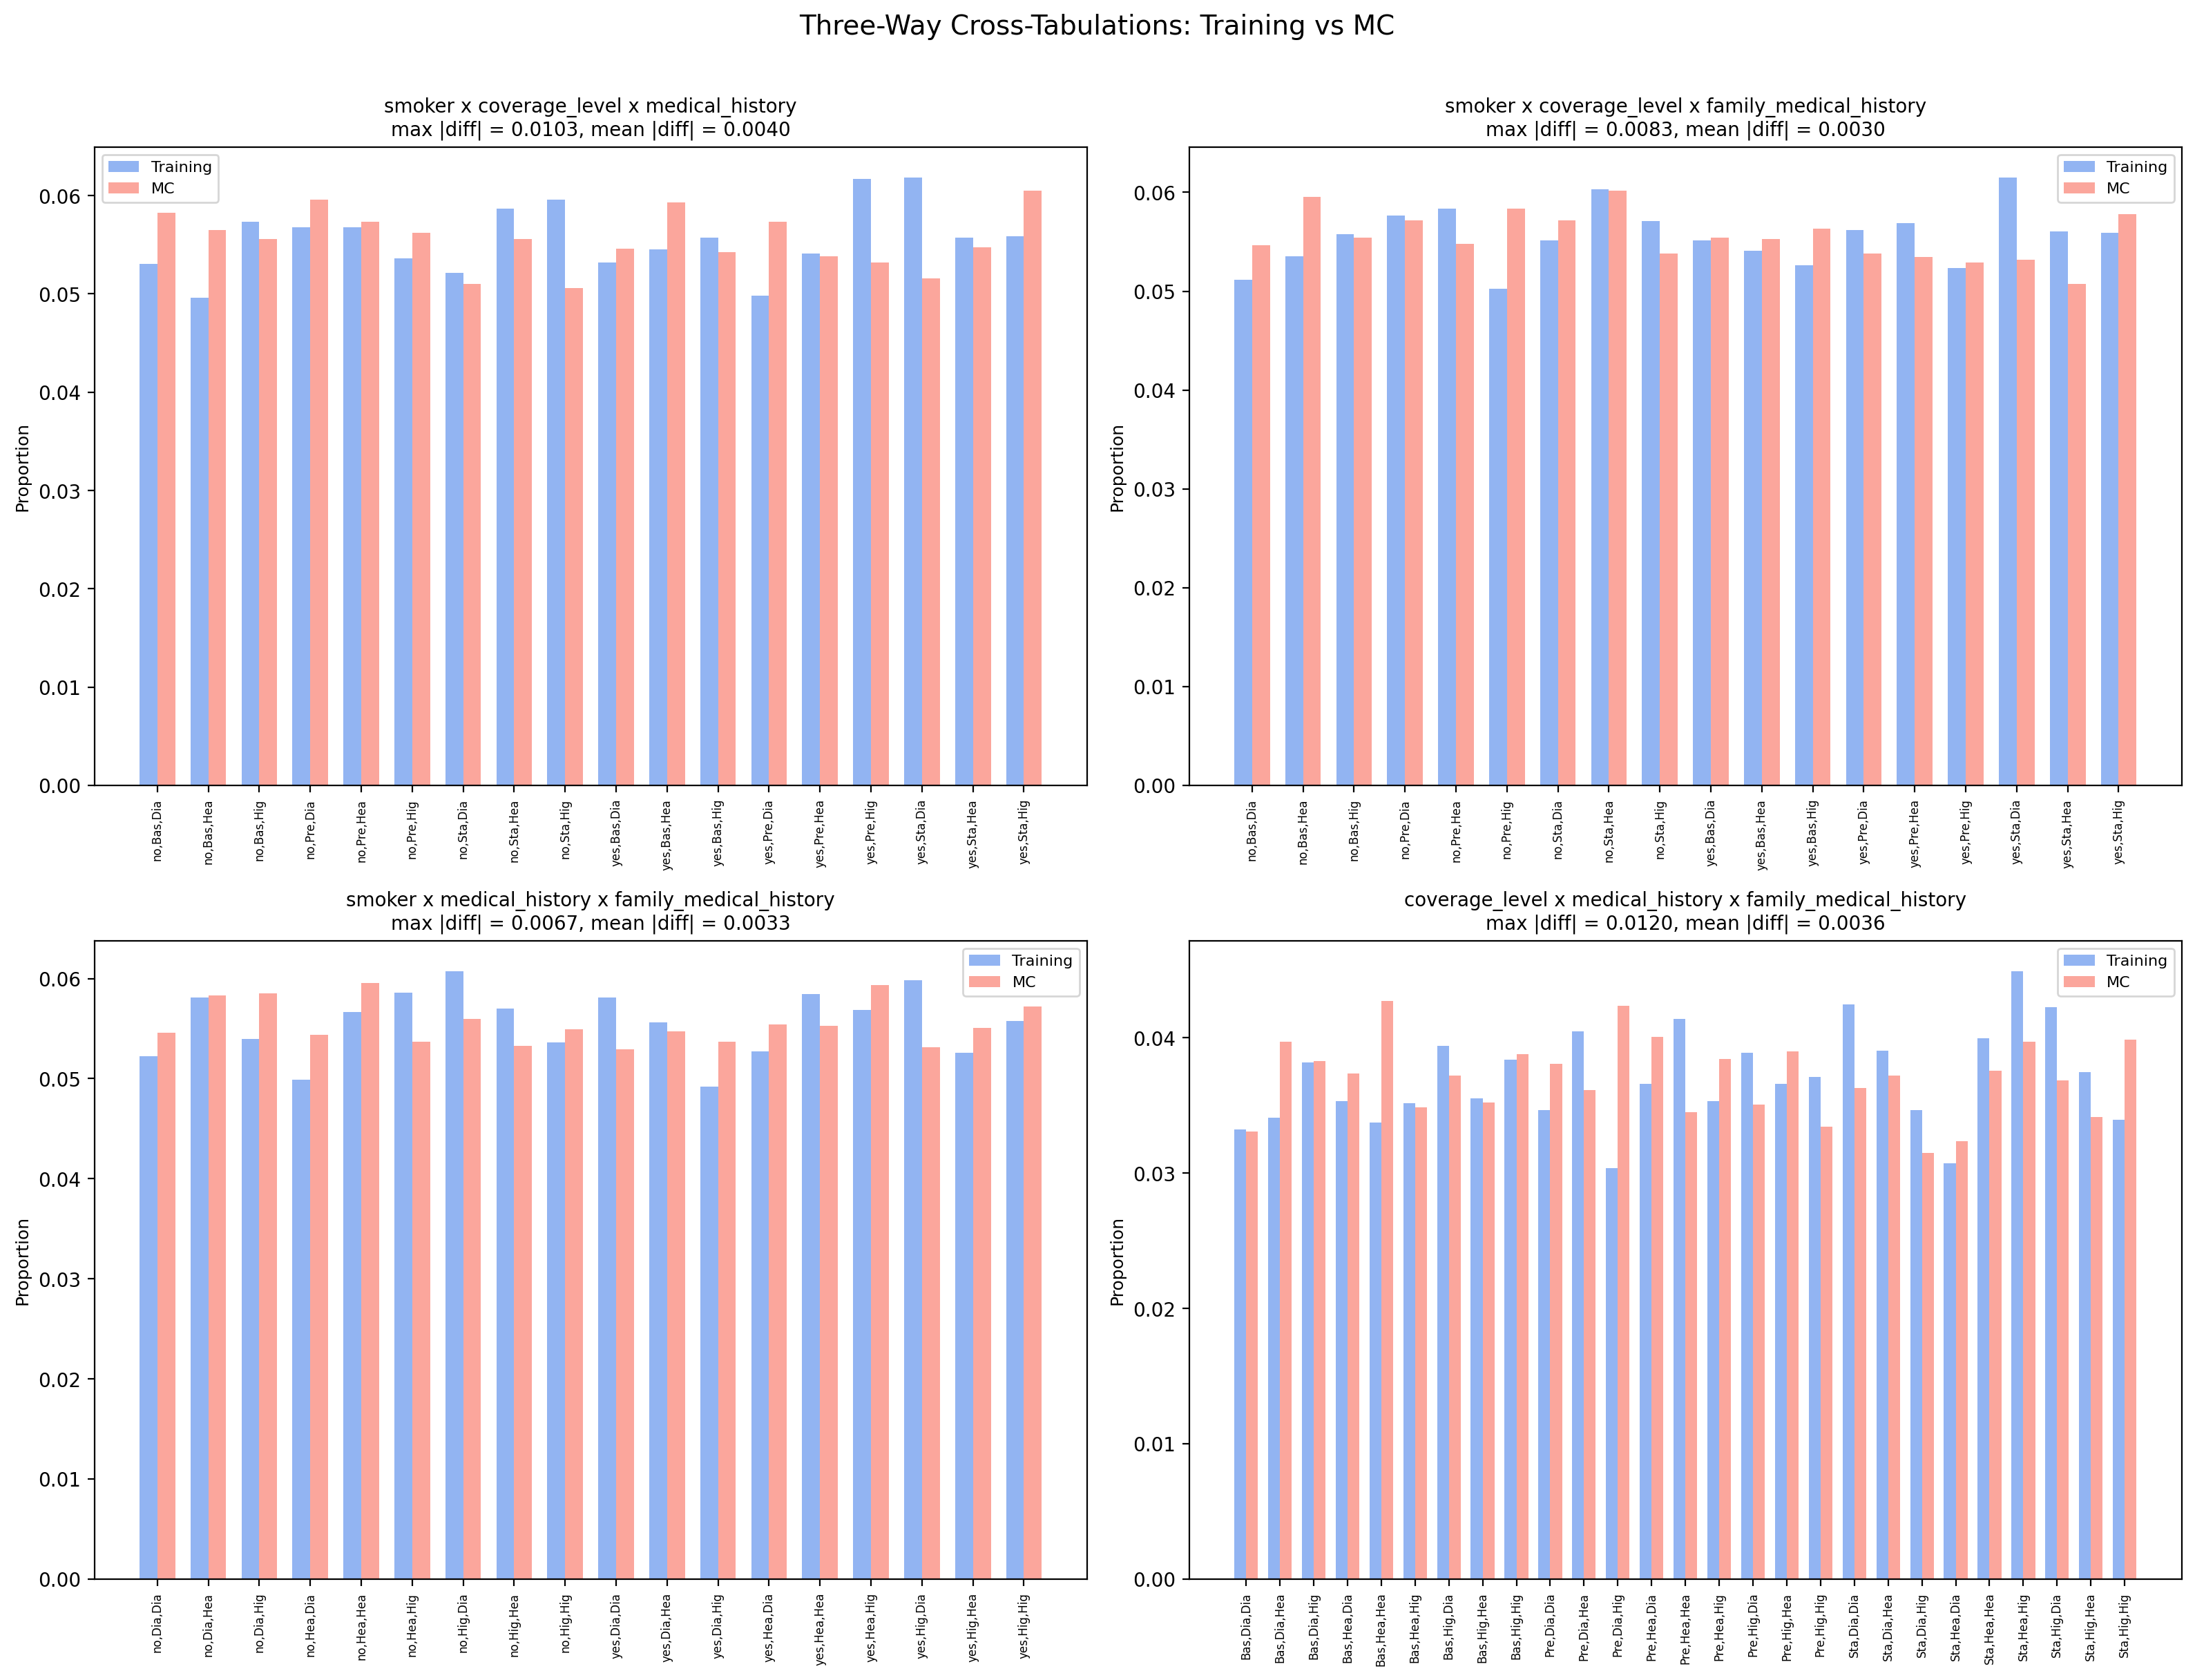
\includegraphics[width=0.95\textwidth]{Thesis/Chapter 4/Figures/fig_threeway_crosstabs.png}
\caption{Three-way cross-tabulations of the four key categorical
variables: training (blue) versus Monte Carlo (red).}
\label{fig:threeway_crosstabs_ch4}
\end{figure}

\noindent
Figure~\ref{fig:threeway_crosstabs_ch4} presents four three-way
cross-tabulations.  Across all triplets, the maximum absolute difference
between the training and Monte Carlo joint proportions is $0.012$
(\texttt{coverage\_level} $\times$ \texttt{medical\_history} $\times$
\texttt{family\_medical\_history}), and the mean absolute differences
are between $0.003$ and $0.004$.  The near-uniform joint proportions in
the training data confirm that higher-order interactions among the
categorical variables are negligible, and the product-marginal
simulation does not discard meaningful multi-way dependence.

\subsubsection*{Multivariate two-sample test}

As a formal test of the overall joint-distribution similarity, the
energy distance between the training and Monte Carlo samples was
computed.

\begin{figure}[H]
\centering
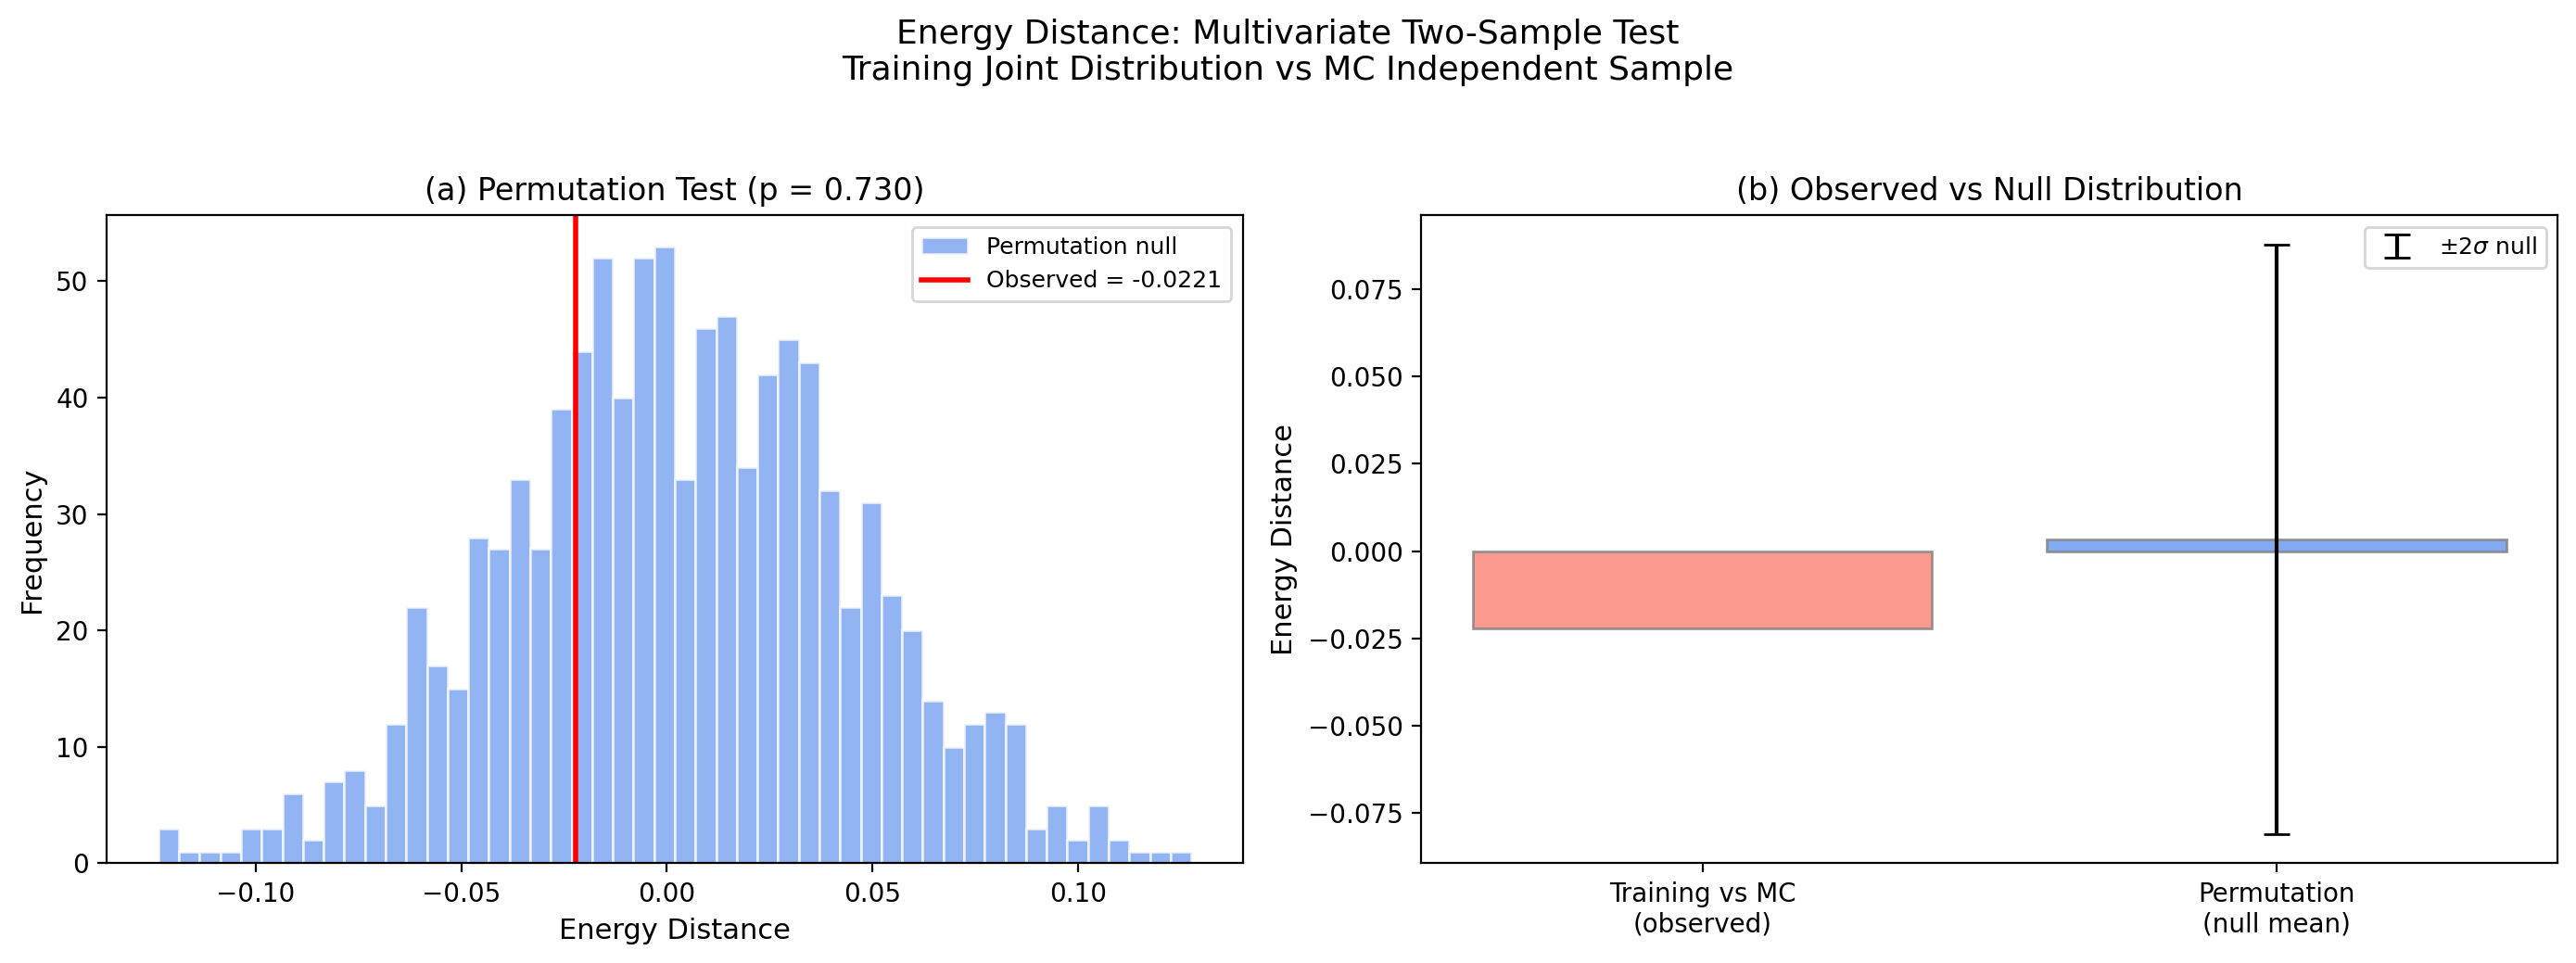
\includegraphics[width=0.95\textwidth]{Thesis/Chapter 4/Figures/fig_energy_distance_test.png}
\caption{Energy distance permutation test: null distribution and observed statistic.}
\label{fig:energy_distance_ch4}
\end{figure}

\noindent
Figure~\ref{fig:energy_distance_ch4} reports the result of a
permutation-based energy distance test with $1\,000$ permutations.  The
observed energy distance is $-0.022$, which falls well within the
permutation null distribution (panel~a).  The permutation $p$-value is
$0.730$, indicating that the observed discrepancy between the training
and Monte Carlo joint distributions is not statistically significant.
The observed energy distance is smaller in magnitude than the null
standard deviation ($0.042$), confirming that the joint distributions
are indistinguishable by this non-parametric criterion.

\subsubsection*{Non-linear manifold overlay}

\begin{figure}[H]
\centering
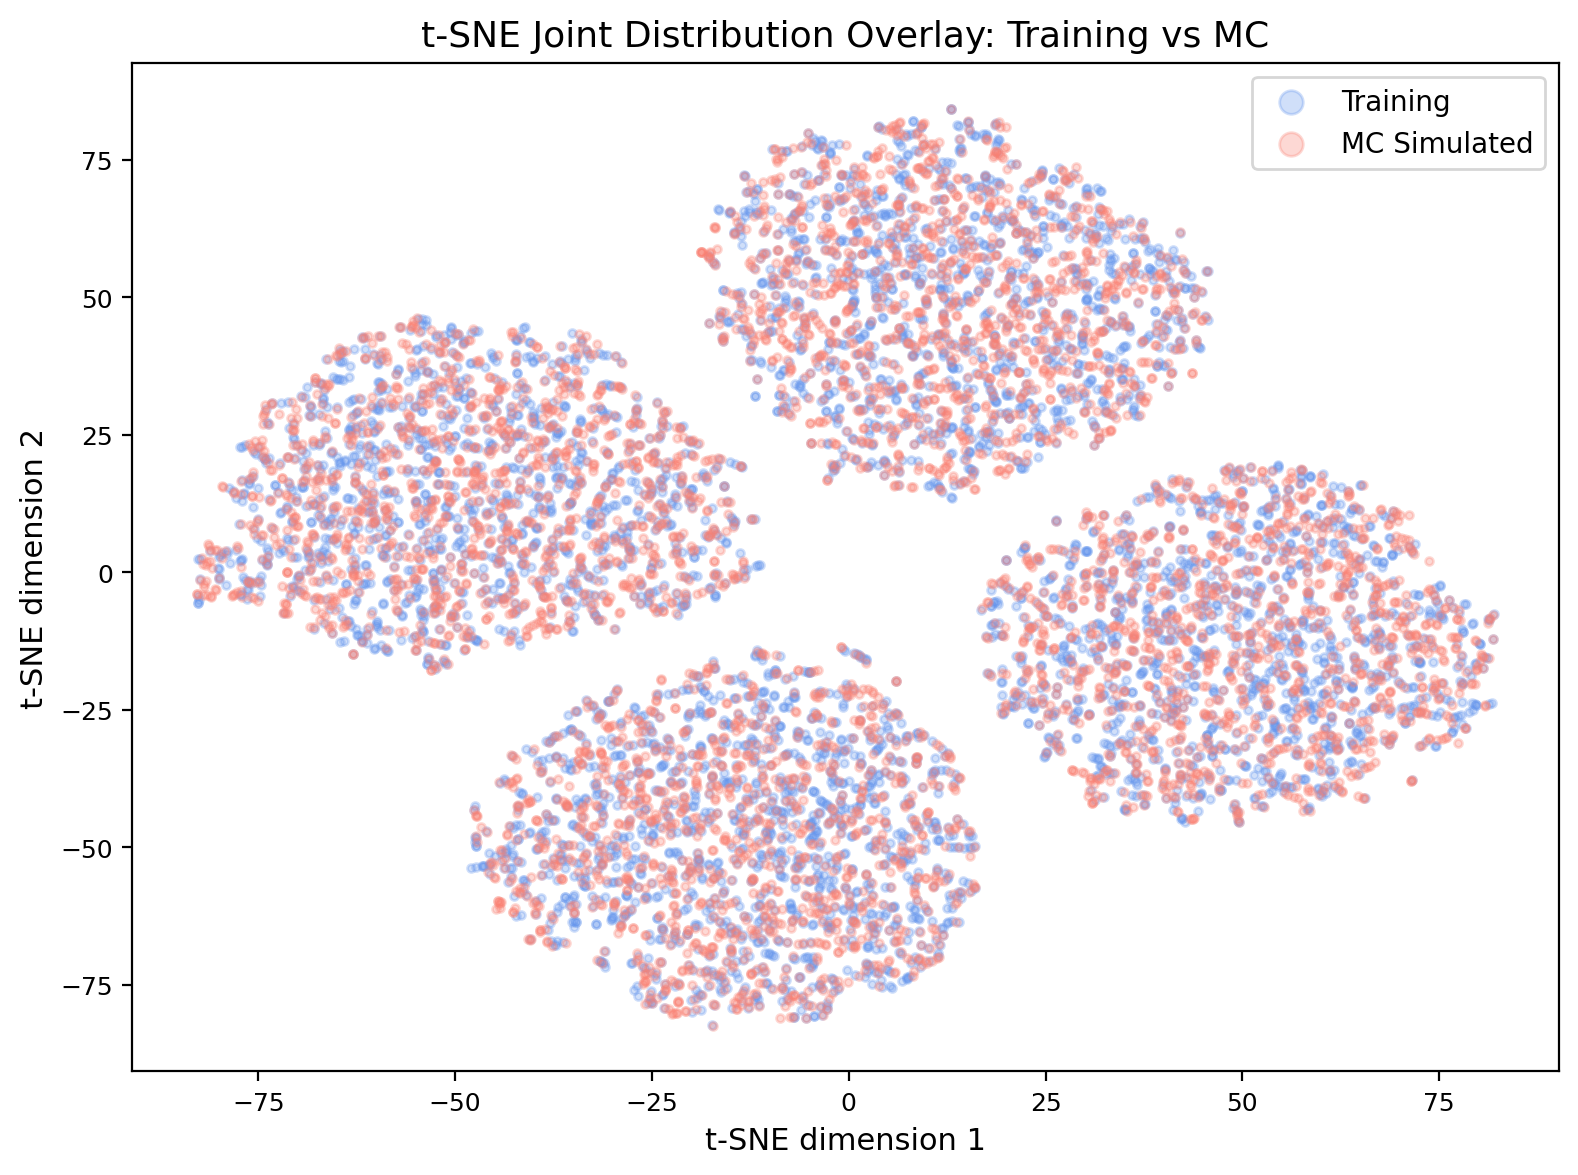
\includegraphics[width=0.70\textwidth]{Thesis/Chapter 4/Figures/fig_tsne_joint_overlay.png}
\caption{t-SNE projection of training versus Monte Carlo joint distributions.}
\label{fig:tsne_joint_overlay_ch4}
\end{figure}

\noindent
Figure~\ref{fig:tsne_joint_overlay_ch4} provides a non-linear
complement to the linear PCA overlay reported in
Section~\ref{sec:mc_input_validation}.  The t-SNE projection maps both
the training and Monte Carlo profiles into two dimensions, preserving
local neighbourhood structure.  The resulting point clouds are
thoroughly intermixed across all identified clusters.  No region of the
manifold is dominated by one sample, confirming that the Monte Carlo
profiles do not occupy novel regions of the feature space that are
unrepresented in the training data.  This result, combined with the PCA
overlay, the energy distance test ($p = 0.730$), and the three-way
cross-tabulations, provides converging evidence that the
product-marginal independence assumption does not materially distort the
joint distributional structure of the training data.

\subsubsection*{Marginal distributions}

\begin{figure}[H]
\centering
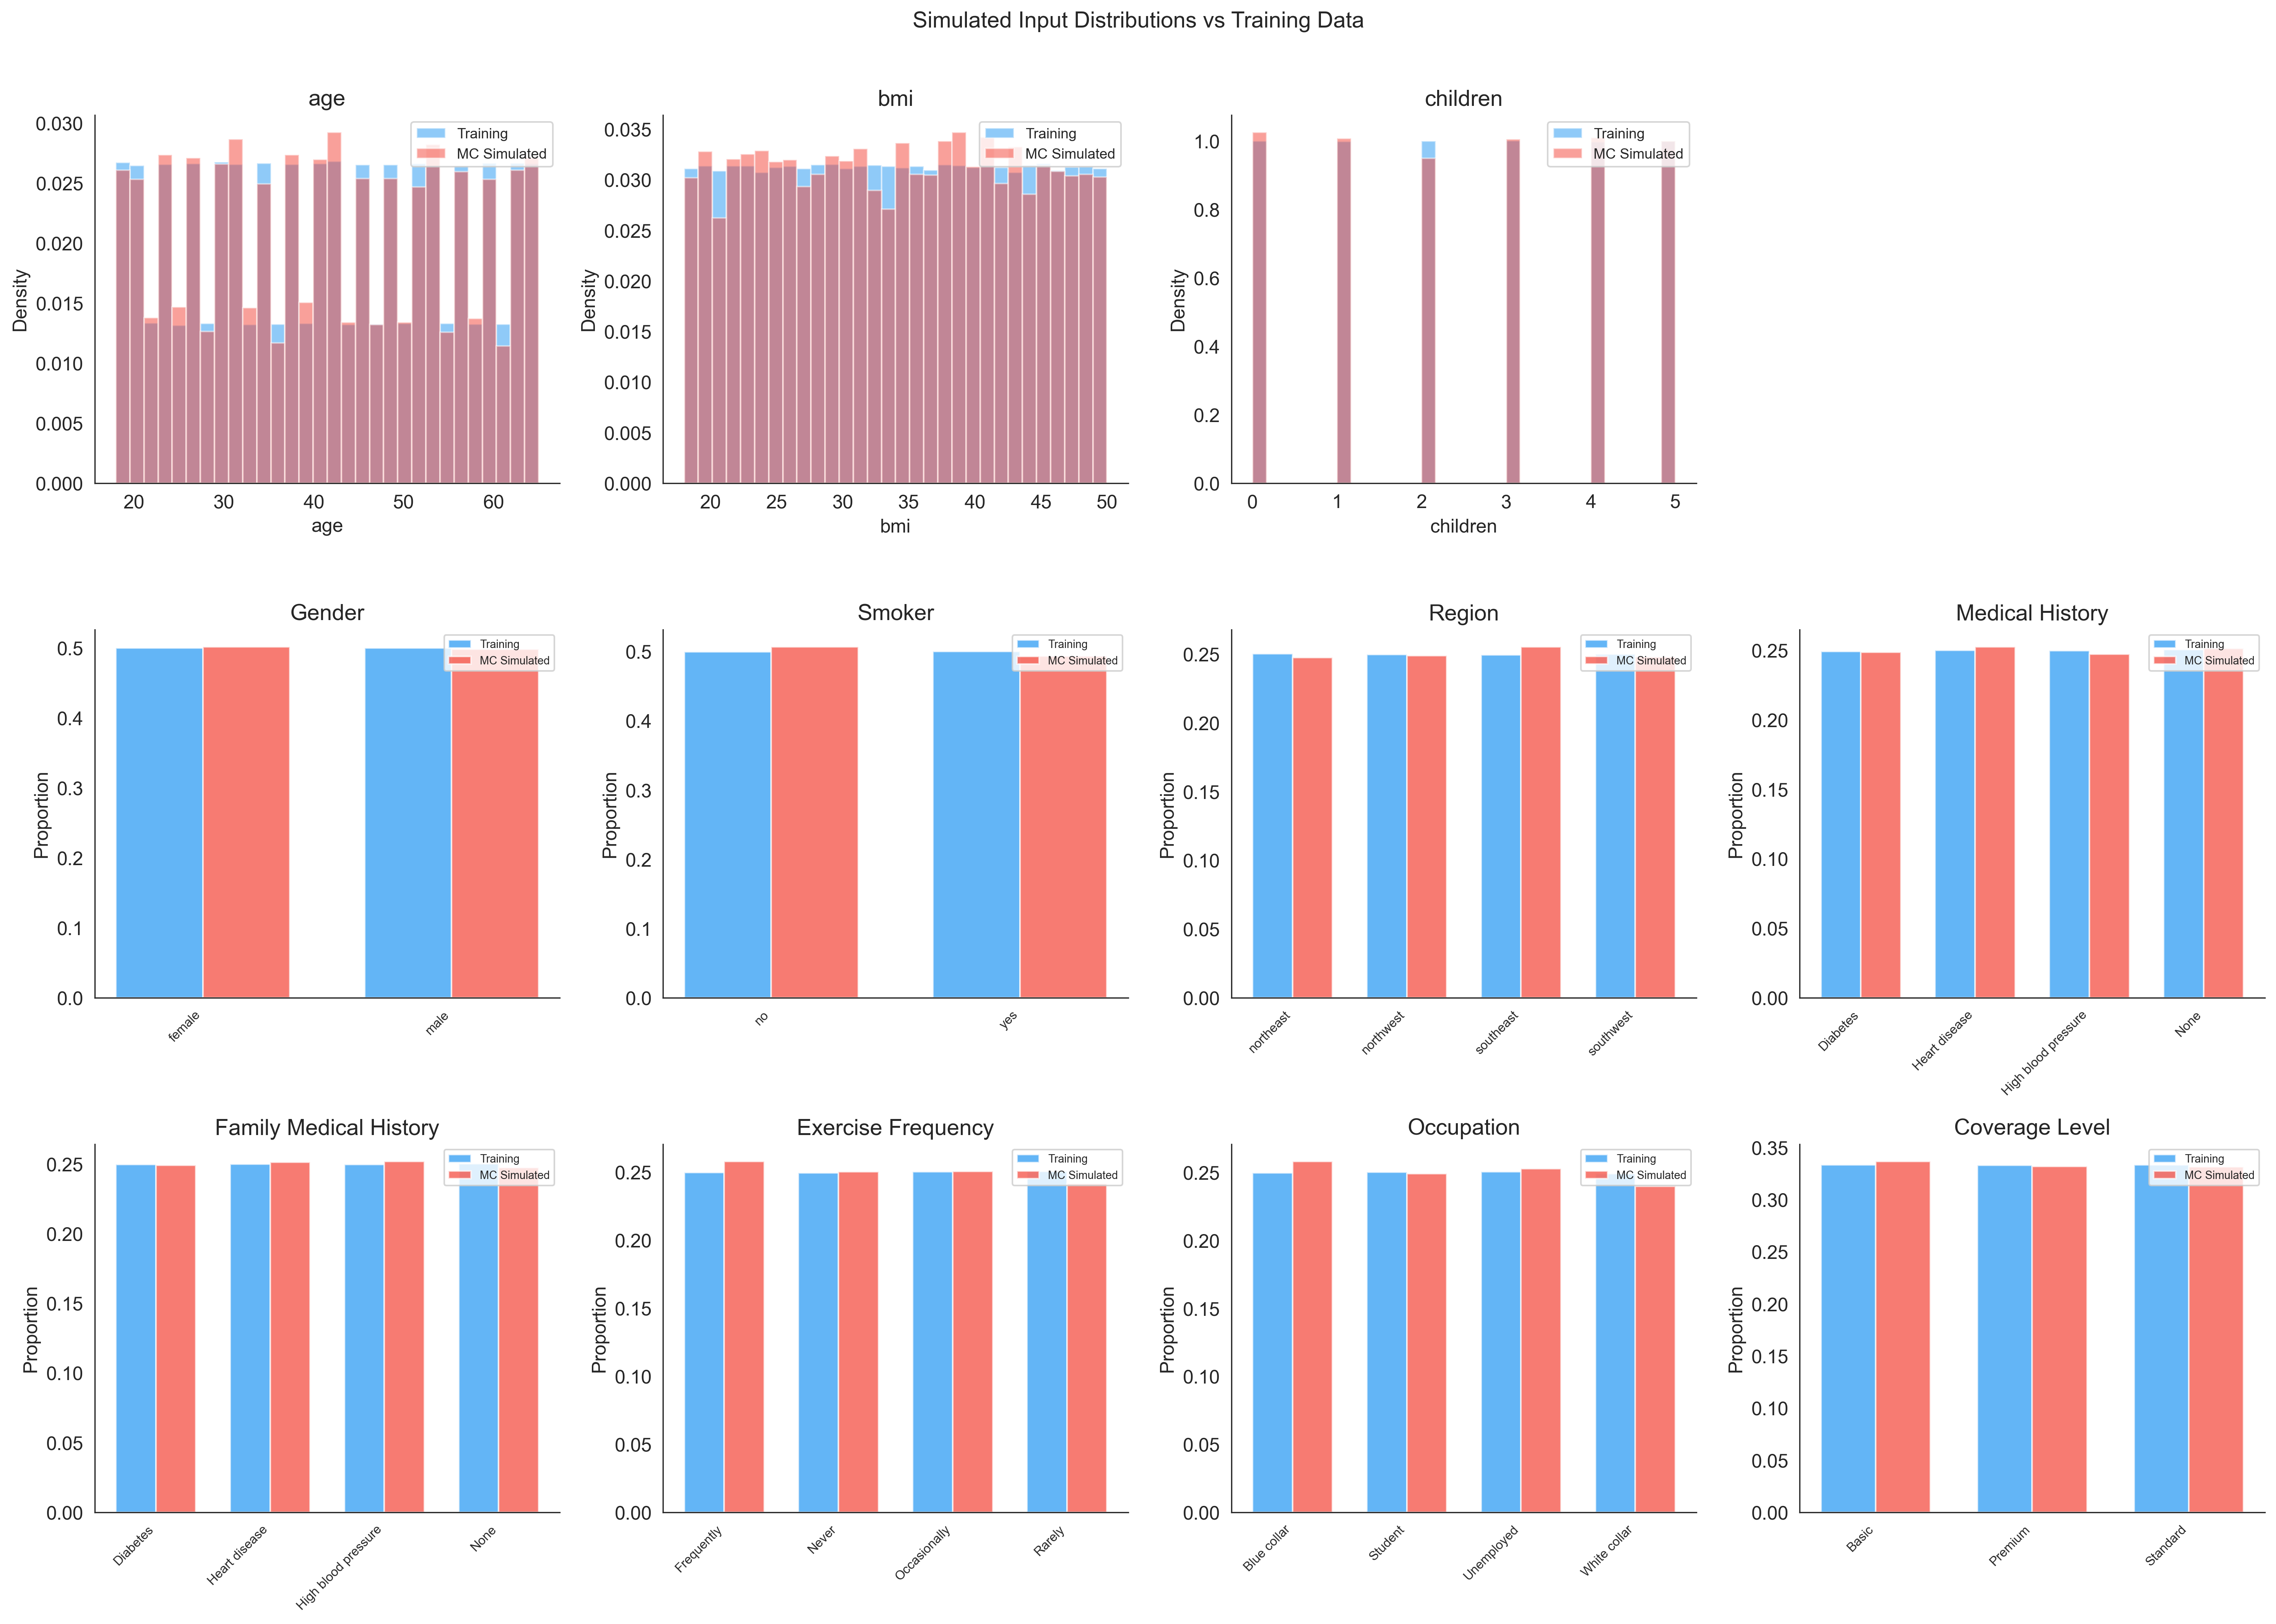
\includegraphics[width=0.95\textwidth]{Thesis/Chapter 4/Figures/fig_mc_input_distributions.png}
\caption{Marginal distributions of all 11 raw predictor variables: training versus Monte Carlo.}
\label{fig:mc_input_distributions_ch4}
\end{figure}

\noindent
Figure~\ref{fig:mc_input_distributions_ch4} confirms that the simulated
marginals closely match the training-data marginals for all 11
variables.  The continuous variables (\texttt{age}, \texttt{bmi}) show
near-uniform histograms in both samples; the discrete count variable
(\texttt{children}) reproduces the approximately equal proportions
across levels 0--5.  For all binary and categorical variables, the
simulated category proportions closely match the training-set
proportions estimated via
equation~\eqref{eq:categorical_probability_estimator_ch3}.  The
parametric simulation therefore faithfully implements the distributional
assumptions stated in Table~\ref{tab:mc_distribution_assumptions_ch3},
at both the joint and marginal levels.

\subsubsection{Model-implied cost distribution}

\begin{figure}[H]
\centering
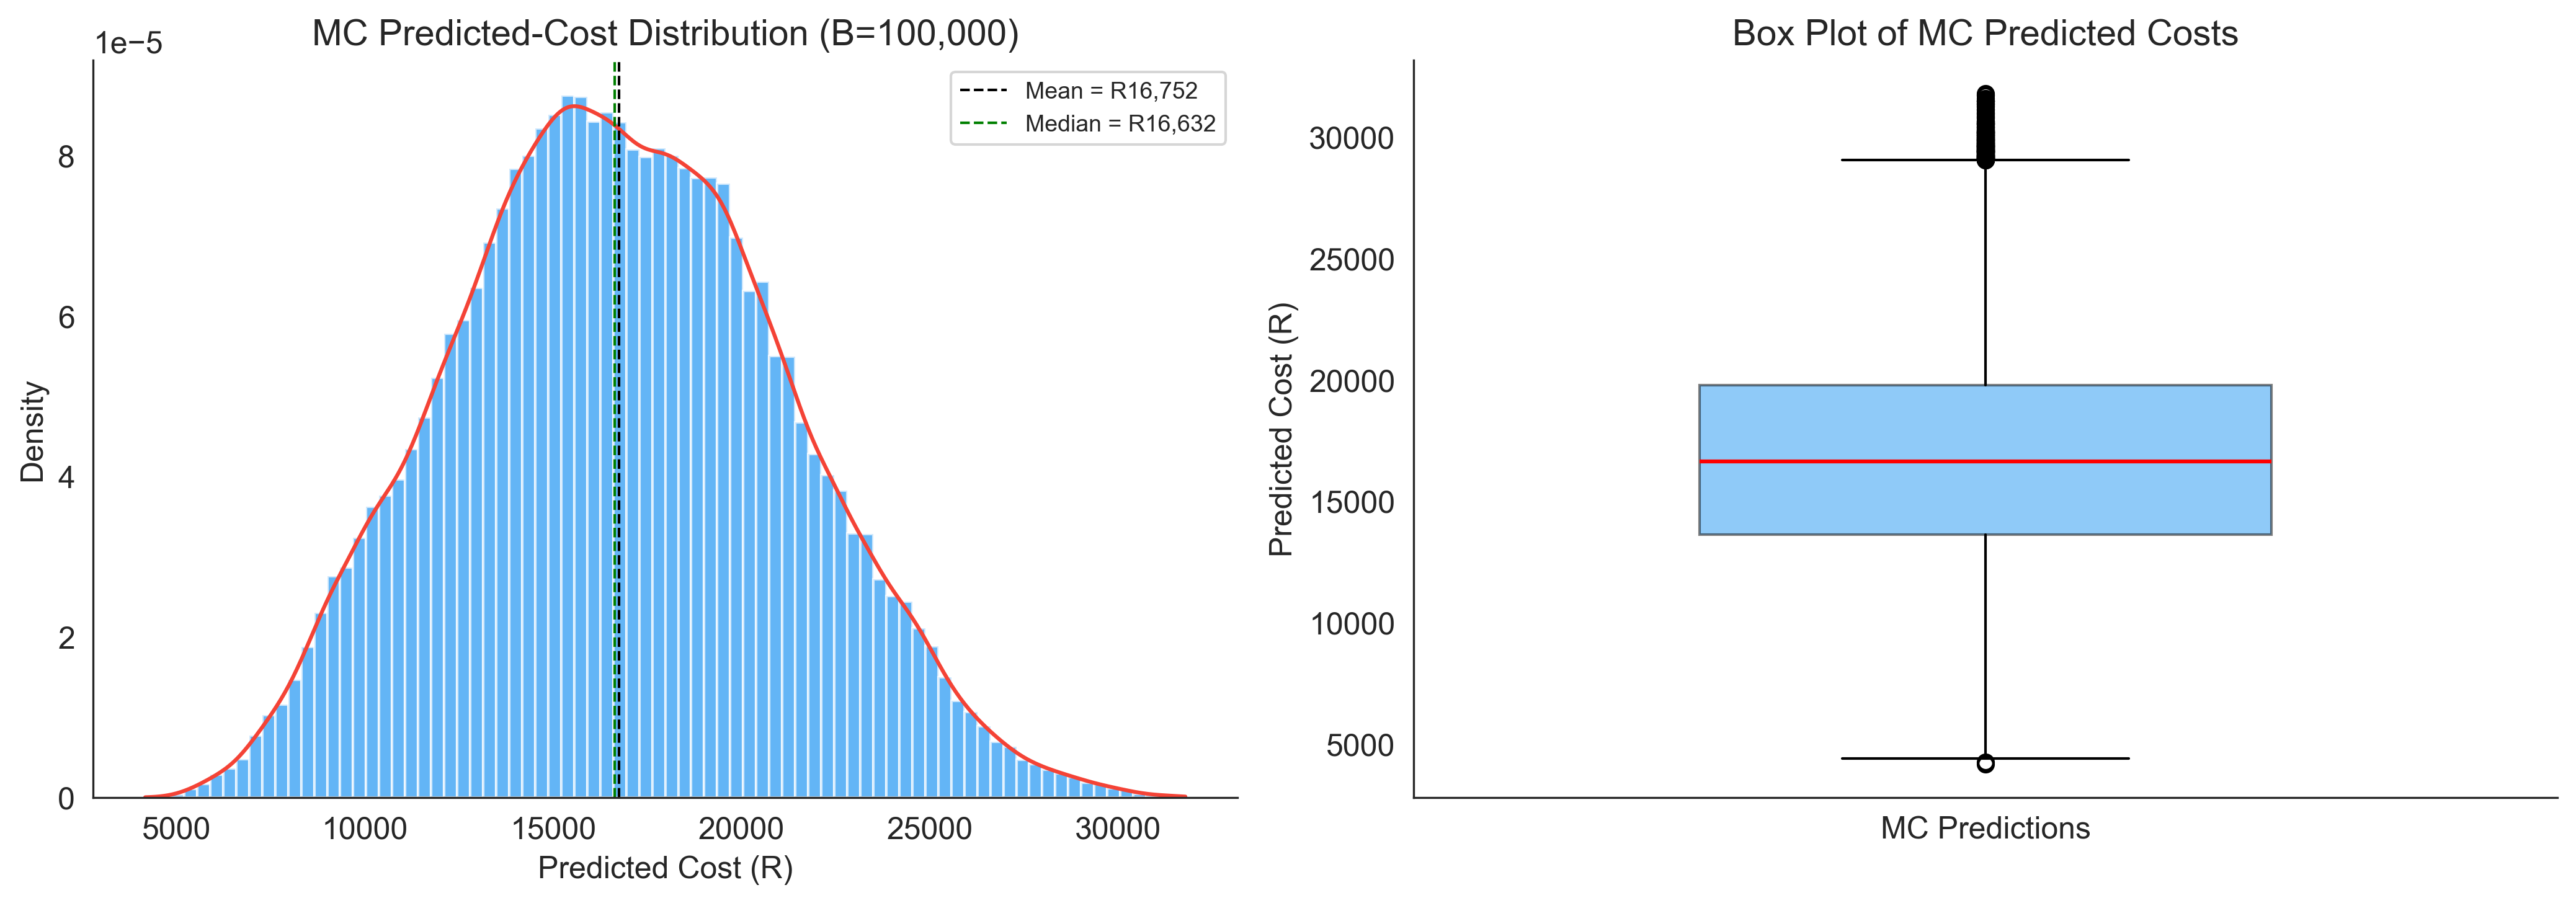
\includegraphics[width=0.95\textwidth]{Thesis/Chapter 4/Figures/fig_mc_predicted_cost_distribution.png}
\caption{Monte Carlo predicted-cost distribution ($B = 10\,000$):
histogram with kernel density overlay (left) and box plot (right).}
\label{fig:mc_predicted_cost_distribution_ch4}
\end{figure}

\noindent
Figure~\ref{fig:mc_predicted_cost_distribution_ch4} displays the
model-implied distribution of predicted insurance costs.
Table~\ref{tab:mc_distribution_summary_ch4} reports the distributional
summary statistics.

\begin{table}[H]
\centering
\caption{Distributional summary of the Monte Carlo predicted costs
($B = 10\,000$).}
\label{tab:mc_distribution_summary_ch4}
\small
\renewcommand{\arraystretch}{1.15}
\begin{tabular}{lr}
\toprule
\textbf{Statistic} & \textbf{Value} \\
\midrule
Mean & R16\,707 \\
Standard deviation & R4\,409 \\
Skewness & $0.128$ \\
Kurtosis & $-0.304$ \\
Minimum & R5\,172 \\
25th percentile & R13\,612 \\
Median & R16\,632 \\
75th percentile & R19\,694 \\
90th percentile & R22\,482 \\
95th percentile & R24\,154 \\
99th percentile & R27\,160 \\
Maximum & R31\,466 \\
\bottomrule
\end{tabular}
\end{table}

\noindent
The distribution is approximately symmetric (skewness $= 0.128$) and
slightly platykurtic (kurtosis $= -0.304$), with a mean of R16\,707 and
a standard deviation of R4\,409. The interquartile range spans
R13\,612 to R19\,694, and the upper tail extends to a maximum predicted
cost of R31\,466. The near-zero skewness and the close agreement
between the mean and median (R16\,707 versus R16\,632) indicate that
the predicted-cost distribution is centred, without heavy-tailed
distortion.

\subsubsection{Convergence diagnostics}

The Monte Carlo standard error and running distributional summaries were
recorded at increasing simulation sizes
$B \in \{1\,000,\; 2\,500,\; 5\,000,\; 10\,000,\; 20\,000\}$
following the convergence monitoring procedure in
Section~\ref{sec:mc_simulation_design}.

\begin{figure}[H]
\centering
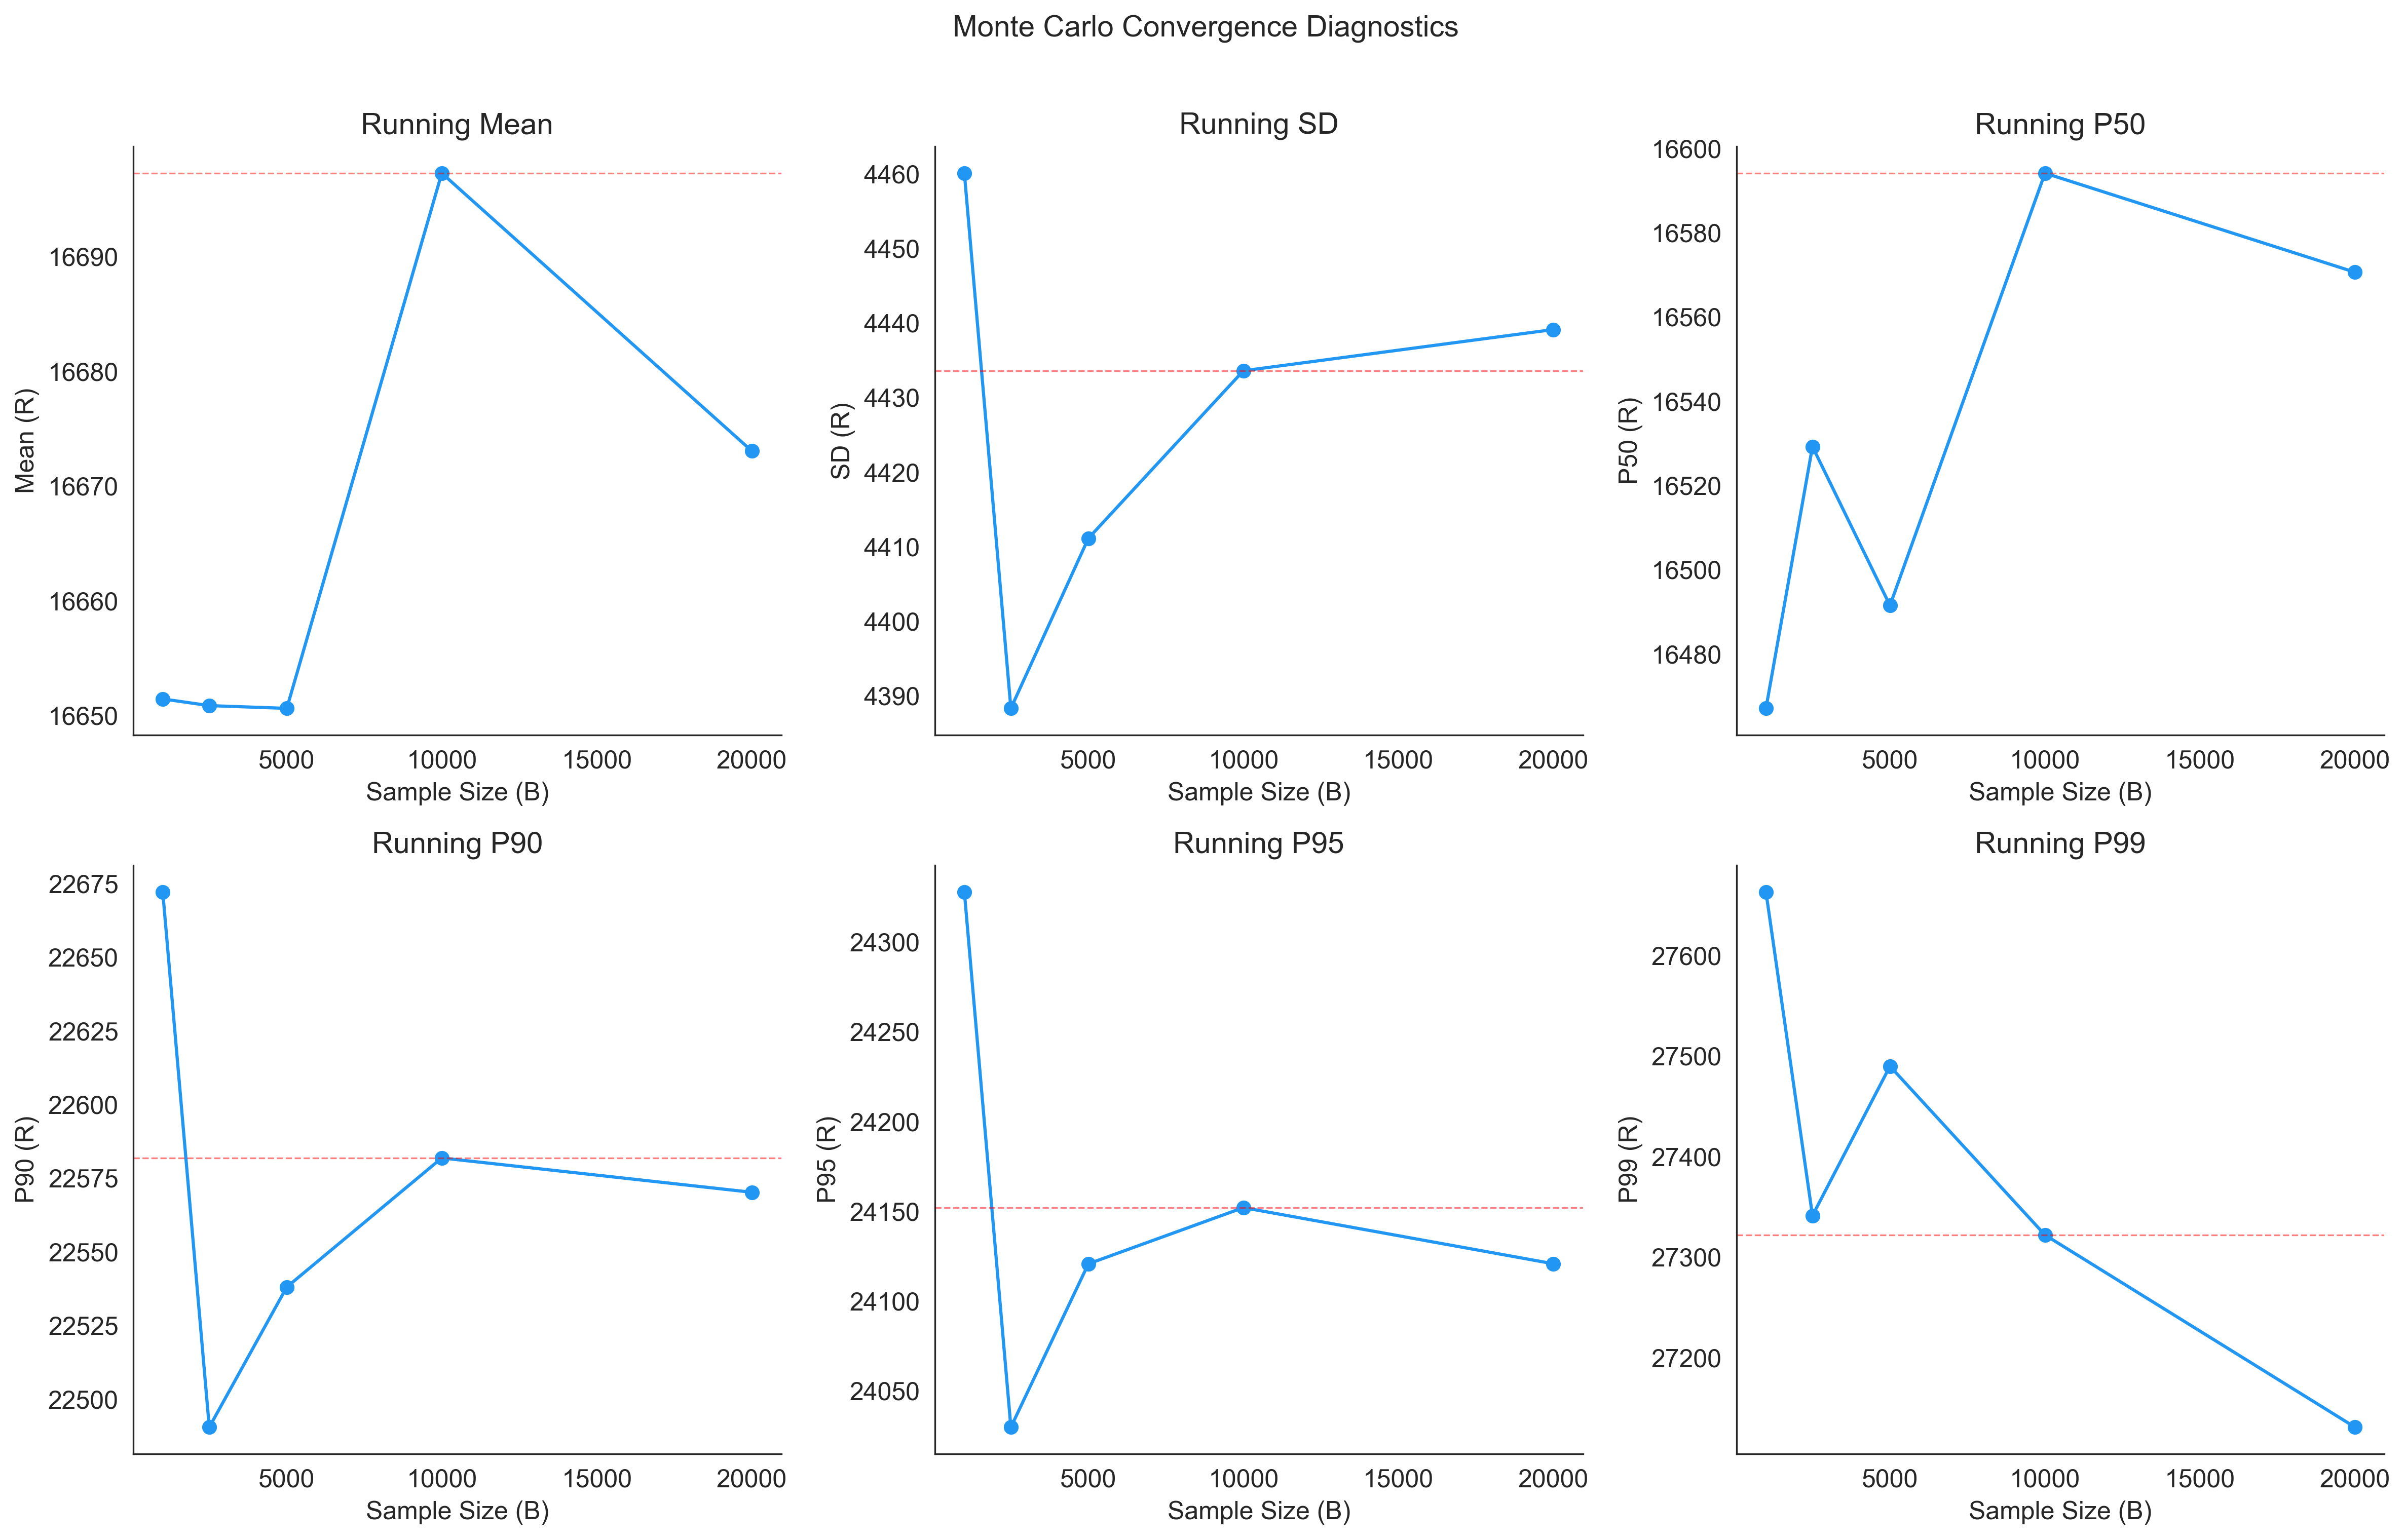
\includegraphics[width=0.95\textwidth]{Thesis/Chapter 4/Figures/fig_mc_convergence.png}
\caption{Monte Carlo convergence diagnostics by simulation size $B$.}
\label{fig:mc_convergence_ch4}
\end{figure}

\noindent
Figure~\ref{fig:mc_convergence_ch4} shows that the running mean
stabilises within a narrow band (R16\,651 to R16\,697) across all
simulation sizes. The running standard deviation converges from R4\,460
at $B = 1\,000$ to R4\,439 at $B = 20\,000$. The median and upper-tail
quantiles exhibit similar stability, with the 95th percentile ranging
from R24\,030 to R24\,328 across all sizes.
Table~\ref{tab:mc_convergence_ch4} reports the \gls{mcse} at each
simulation size.

\begin{table}[H]
\centering
\caption{Monte Carlo convergence: running summaries and MCSE by
simulation size.}
\label{tab:mc_convergence_ch4}
\small
\renewcommand{\arraystretch}{1.15}
\begin{tabular}{rrrrrrrr}
\toprule
$B$ & Mean & SD & Median & P90 & P95 & P99 & MCSE \\
\midrule
1\,000 & 16\,651 & 4\,460 & 16\,467 & 22\,672 & 24\,328 & 27\,663 & 141.0 \\
2\,500 & 16\,651 & 4\,388 & 16\,529 & 22\,490 & 24\,030 & 27\,341 & 87.8 \\
5\,000 & 16\,651 & 4\,411 & 16\,492 & 22\,538 & 24\,121 & 27\,490 & 62.4 \\
10\,000 & 16\,697 & 4\,434 & 16\,594 & 22\,582 & 24\,152 & 27\,322 & 44.3 \\
20\,000 & 16\,673 & 4\,439 & 16\,571 & 22\,570 & 24\,121 & 27\,131 & 31.4 \\
\bottomrule
\end{tabular}
\end{table}

\noindent
The \gls{mcse} decreases from R141 at $B = 1\,000$ to R44.3 at
$B = 10\,000$, representing $0.27\%$ of the mean predicted cost. At the
selected simulation size of $B = 10\,000$, the running summaries have
stabilised and the simulation precision is adequate for the subsequent
distributional and attribution analyses.

\subsubsection{Comparison with observed training charges}

\begin{figure}[H]
\centering
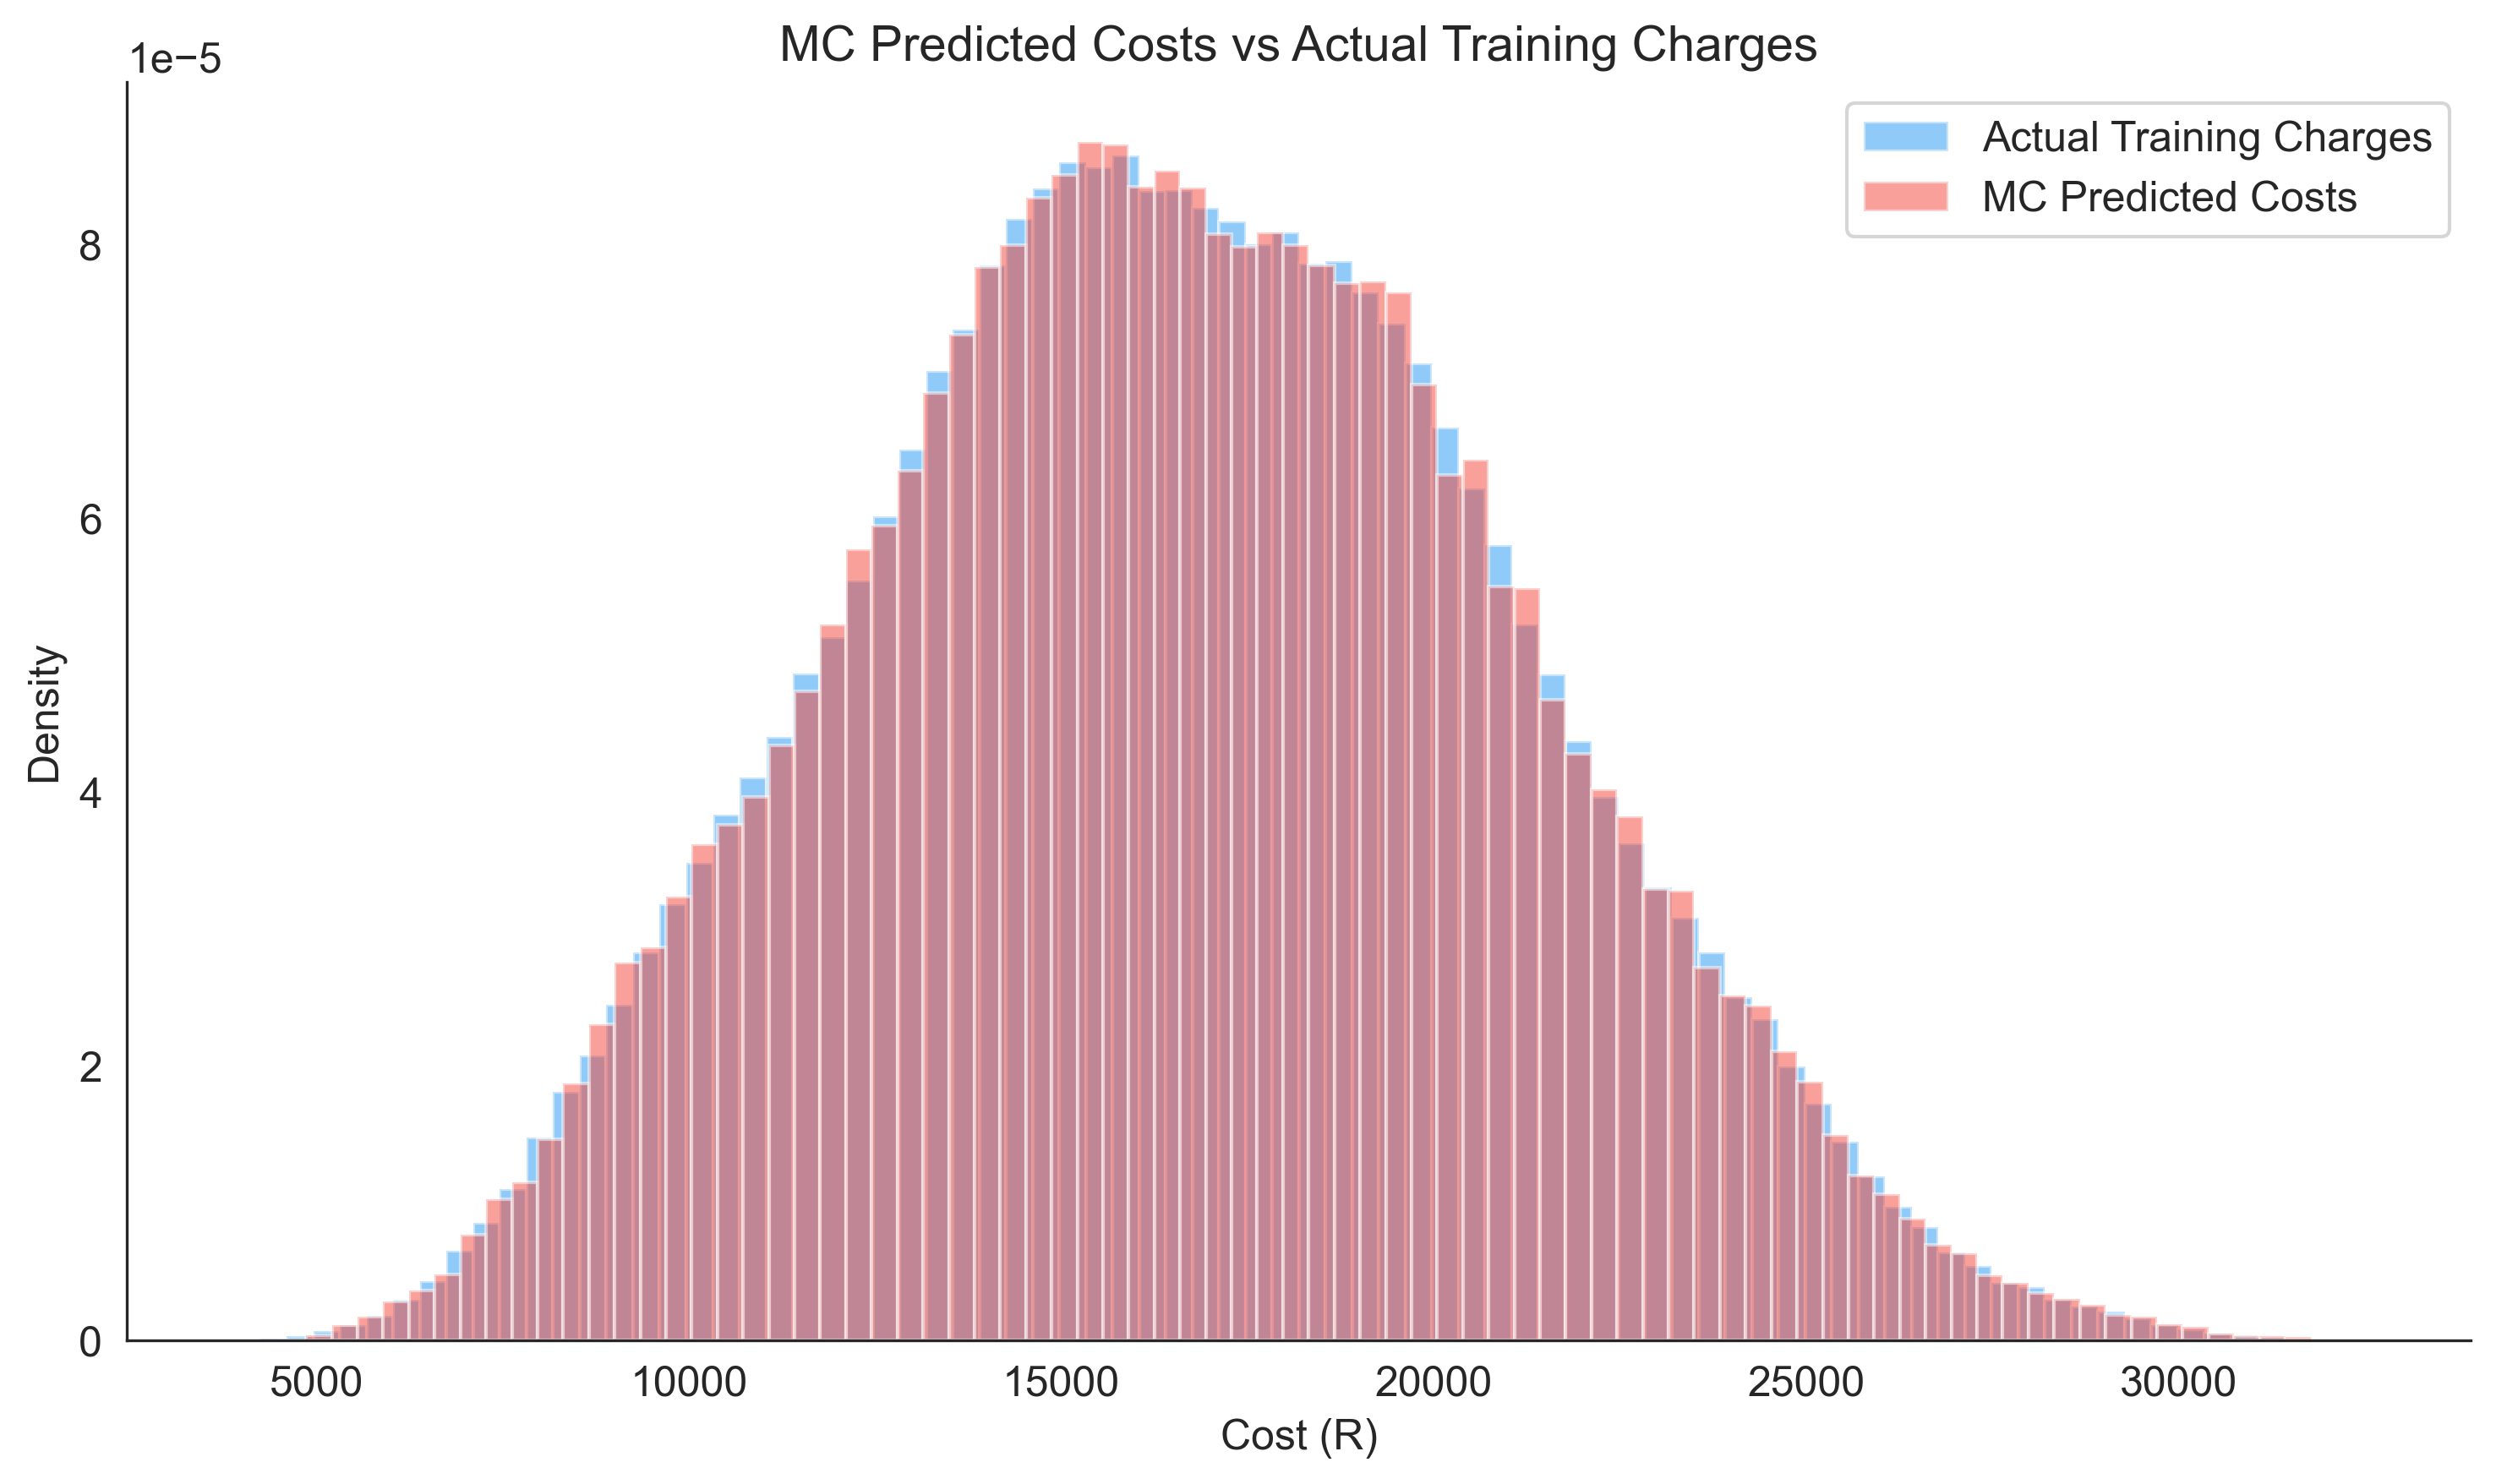
\includegraphics[width=0.80\textwidth]{Thesis/Chapter 4/Figures/fig_mc_predicted_vs_actual.png}
\caption{Overlay of the Monte Carlo predicted-cost distribution (red)
and the observed training-set charge distribution (blue).}
\label{fig:mc_predicted_vs_actual_ch4}
\end{figure}

\noindent
Figure~\ref{fig:mc_predicted_vs_actual_ch4} overlays the Monte Carlo
predicted-cost histogram with the observed training-set charge
distribution. The two distributions share similar location, spread and
shape: both are unimodal, roughly symmetric, and span the range from
approximately R5\,000 to R32\,000. The close agreement confirms that
the fitted \gls{dnn}, when evaluated on profiles drawn from the
parametric input distribution, produces a predicted-cost landscape that
is consistent with the distributional characteristics of the observed
training data. Minor differences in the tails reflect the smoothing
behaviour of the regression model and the slight mismatch between the
product-marginal simulation law and the empirical joint distribution.


% =============================================================
\subsection{Residual-Augmented Monte Carlo Sensitivity}
\label{sec:residual_augmented_results}

The residual-augmented sensitivity analysis
(Section~\ref{sec:residual_augmented_mc}) was applied to the
$B = 10\,000$ base Monte Carlo predictions.  Centred fitted residuals
were drawn from the empirical residual distribution
$\widehat{F}_{\varepsilon}$
(equation~\eqref{eq:residual_draw_ch3}), and a fixed perturbation band
of $\pm 0.5\,\widehat{\sigma}_{\varepsilon}$ was computed following
equation~\eqref{eq:fixed_residual_perturbation_ch3}.

\begin{figure}[H]
\centering
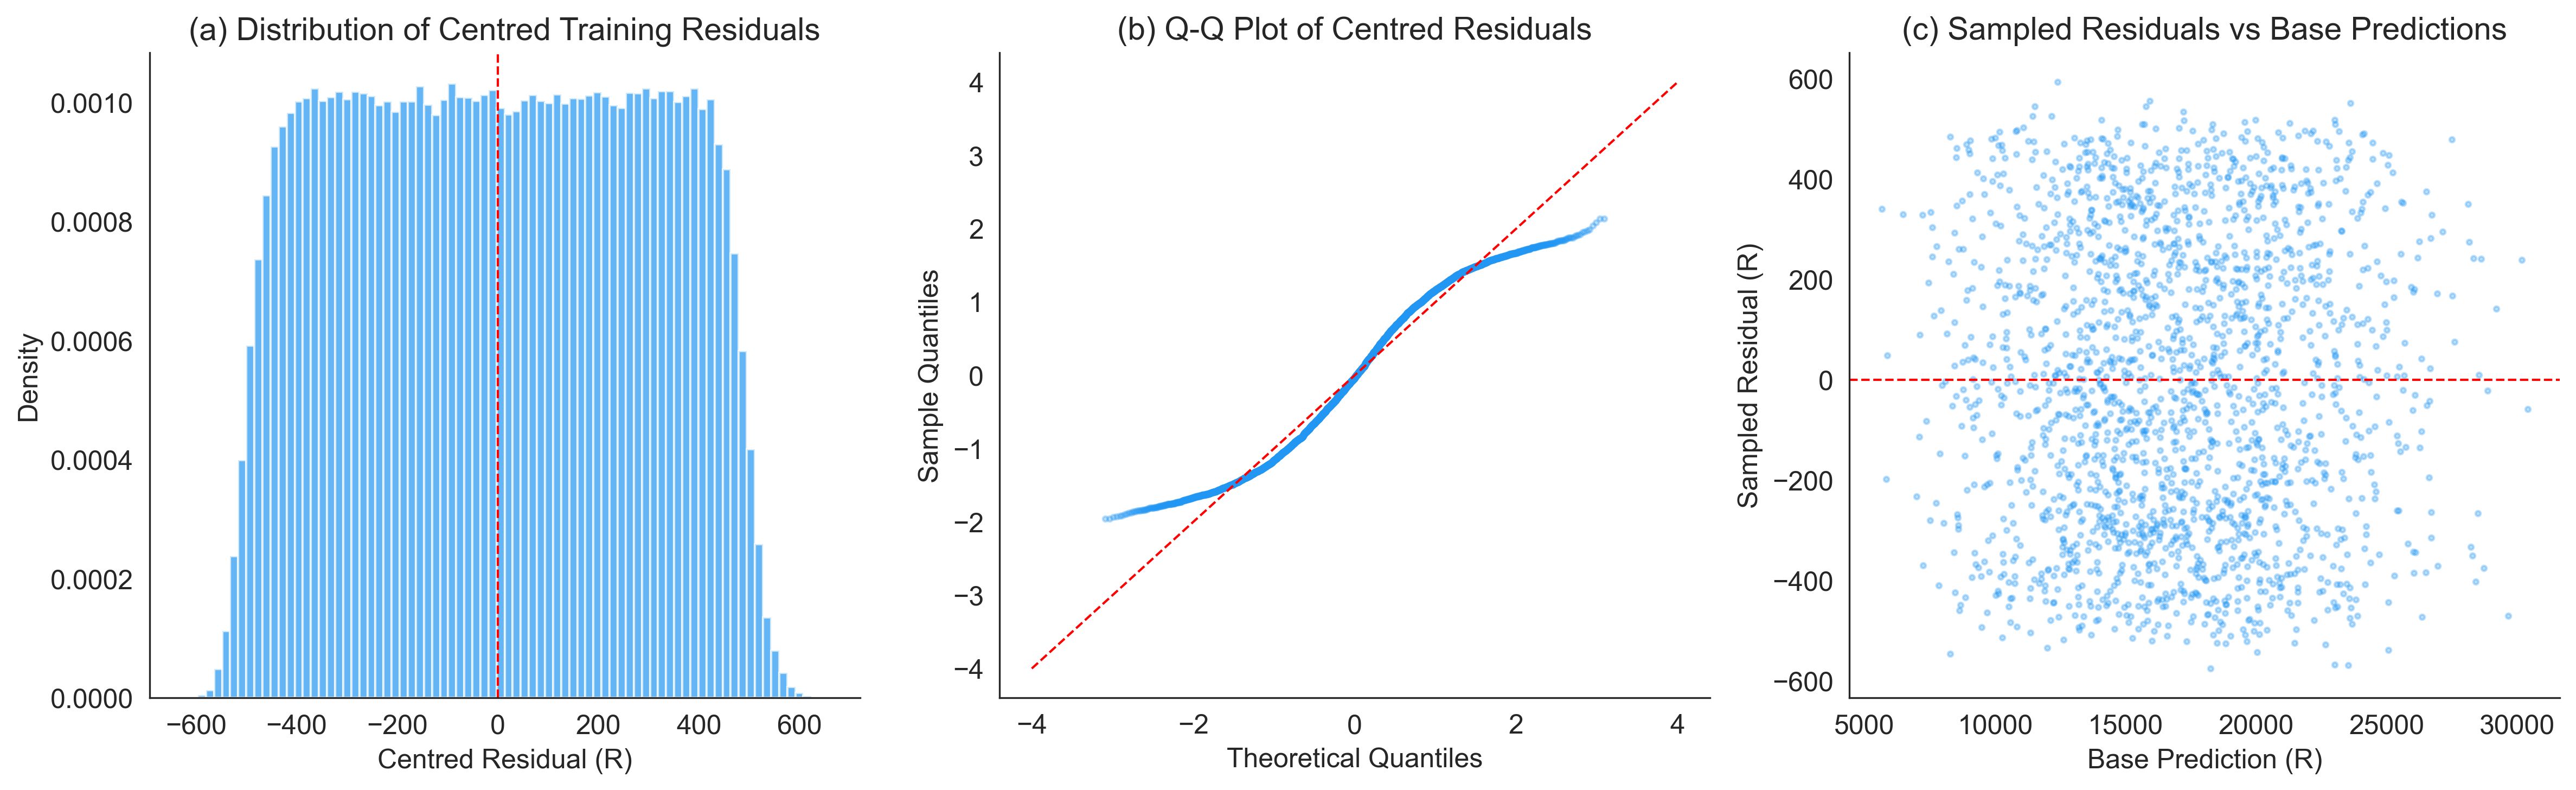
\includegraphics[width=0.95\textwidth]{Thesis/Chapter 4/Figures/fig_mc_residual_diagnostics.png}
\caption{Centred training residual diagnostics for the augmented simulation.}
\label{fig:mc_residual_diagnostics_ch4}
\end{figure}

\noindent
Figure~\ref{fig:mc_residual_diagnostics_ch4} characterises the centred
training residuals from which the augmented draws are sampled.  The
histogram in panel~(a) is symmetric and bell-shaped, confirming that the
residual distribution is well-centred and does not contain systematic
bias.  The Q-Q plot in panel~(b) shows slight tail compression relative
to a Gaussian reference, consistent with the mild platykurtic behaviour
noted in the model diagnostics of
Section~\ref{sec:model_validation_diagnostics}.  Panel~(c) plots the
sampled residuals against the base predictions: the scatter is random
and centred at zero across the full prediction range (R5\,000 to
R30\,000), indicating that the residual magnitude does not depend on the
predicted cost level.  These properties confirm that the empirical
residual distribution is suitable for the perturbation analysis.

\begin{figure}[H]
\centering
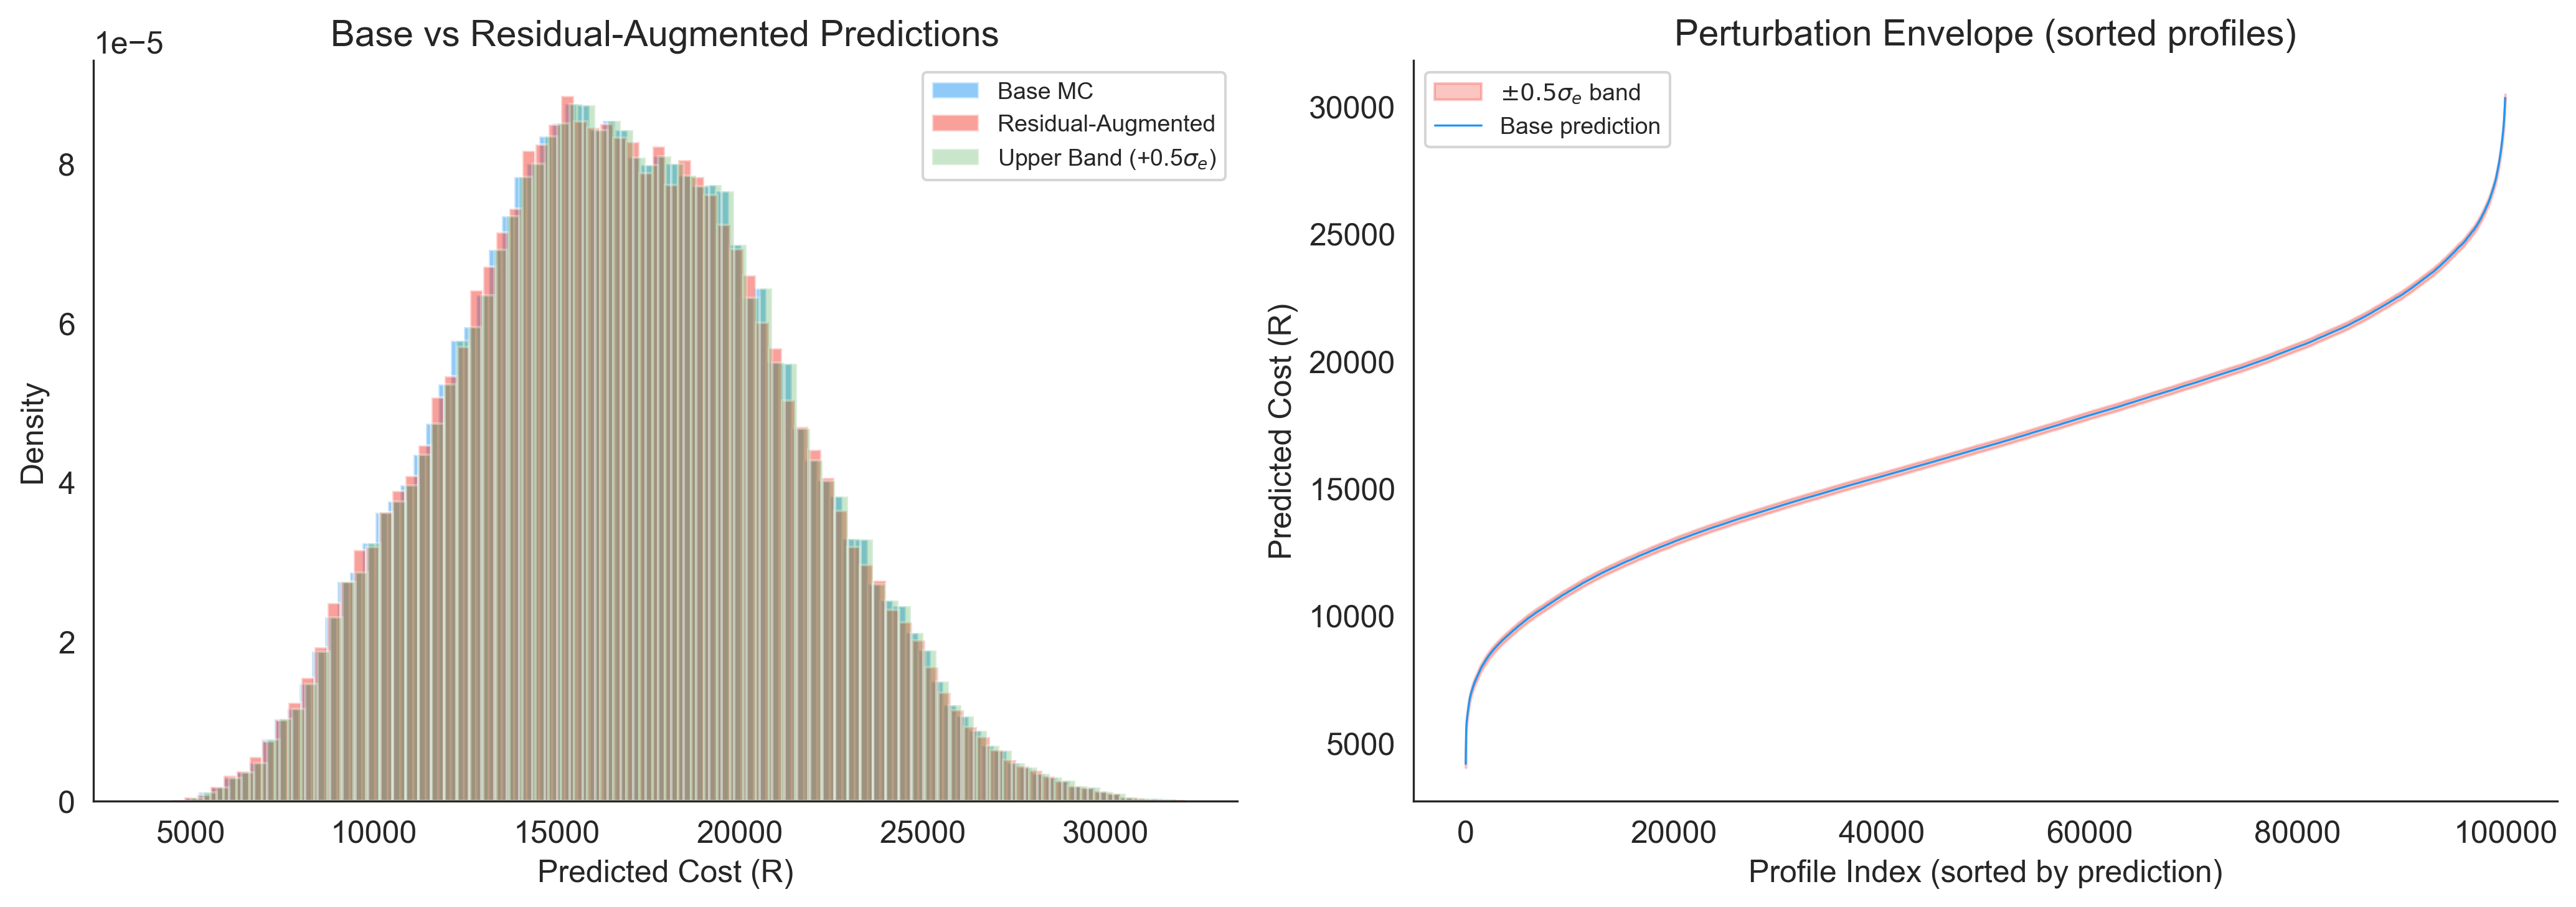
\includegraphics[width=0.95\textwidth]{Thesis/Chapter 4/Figures/fig_mc_residual_augmented.png}
\caption{Residual-augmented Monte Carlo sensitivity analysis.}
\label{fig:mc_residual_augmented_ch4}
\end{figure}

\noindent
Figure~\ref{fig:mc_residual_augmented_ch4} (left panel) shows that the
residual-augmented distribution closely overlaps the base Monte Carlo
distribution. The residual perturbation does not shift the central
tendency or materially alter the distributional shape: the mode, spread
and tail behaviour of all three distributions remain aligned. The right
panel displays the sorted base predictions with the
$\pm 0.5\,\widehat{\sigma}_{\varepsilon}$ perturbation envelope. The
envelope forms a narrow, uniform band around the base prediction curve
across the full range of predicted costs, from approximately R5\,000 at
the lower end to R30\,000 at the upper end. The width of the band
remains constant relative to the prediction magnitude, confirming that
the fitted residual variability is small and homogeneous across the
predicted-cost range.

These results indicate that the distributional conclusions drawn from
the base Monte Carlo analysis are not sensitive to the magnitude of the
fitted model's residual error. The base predicted-cost distribution is
therefore a stable foundation for the Shapley-value attribution analysis
that follows.


% =============================================================
\subsection{Shapley-Value Attribution Results}
\label{sec:shapley_results}

Shapley values were computed for all $B = 10\,000$ simulated
profiles using the gradient-based SHAP explainer described in
Table~\ref{tab:shap_implementation_settings_ch3}. Dummy-level
attributions were aggregated to the raw-variable level ($q = 11$)
using equation~\eqref{eq:raw_variable_shap_aggregation_ch3}.

\subsubsection{Global feature importance}

Global feature importance was assessed using the mean absolute Shapley
value $I_g$ (equation~\eqref{eq:mean_absolute_shap_ch3}) and the mean
signed Shapley value $\overline{\phi}_g$
(equation~\eqref{eq:mean_signed_shap_ch3}), computed over all $B$
simulated profiles.

\begin{figure}[H]
\centering
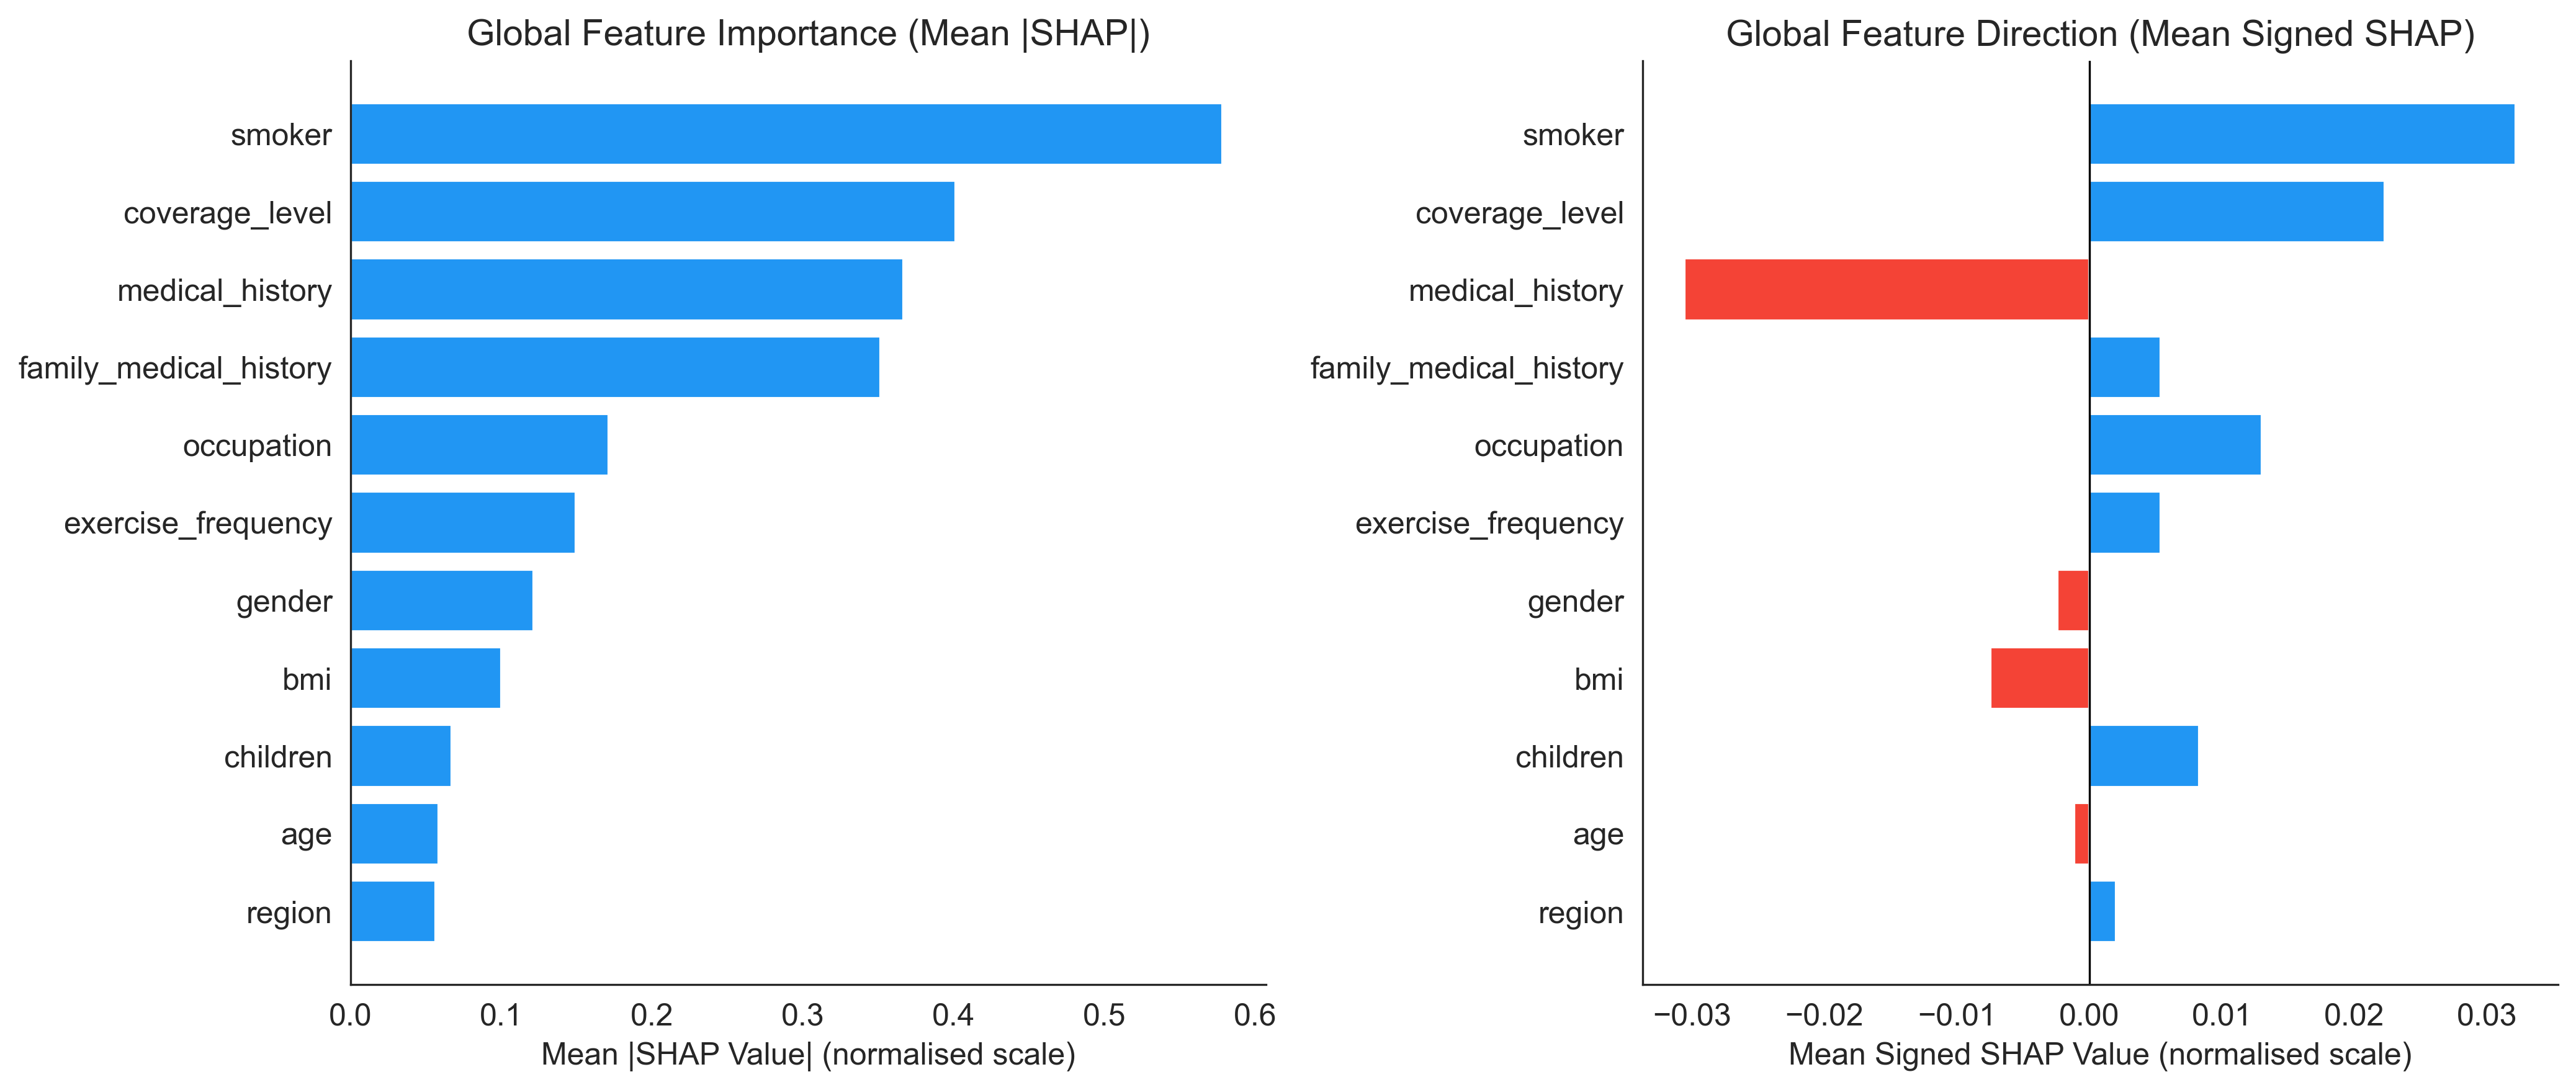
\includegraphics[width=0.95\textwidth]{Thesis/Chapter 4/Figures/fig_shap_global_importance.png}
\caption{Global Shapley feature importance for all 11 raw variables.}
\label{fig:shap_global_importance_ch4}
\end{figure}

\noindent
Figure~\ref{fig:shap_global_importance_ch4} displays the global
feature-importance ranking. Table~\ref{tab:shap_global_importance_ch4}
reports the numerical values.

\begin{table}[H]
\centering
\caption{Global Shapley feature importance: mean signed and mean
absolute values for all 11 raw variables on the normalised scale.}
\label{tab:shap_global_importance_ch4}
\small
\renewcommand{\arraystretch}{1.15}
\begin{tabular}{lrr}
\toprule
\textbf{Variable} & \textbf{Mean signed SHAP} & \textbf{Mean $|\text{SHAP}|$} \\
\midrule
\texttt{smoker} & $+0.022$ & $0.577$ \\
\texttt{coverage\_level} & $+0.020$ & $0.401$ \\
\texttt{medical\_history} & $-0.030$ & $0.368$ \\
\texttt{family\_medical\_history} & $+0.007$ & $0.352$ \\
\texttt{occupation} & $+0.011$ & $0.170$ \\
\texttt{exercise\_frequency} & $+0.009$ & $0.151$ \\
\texttt{gender} & $-0.002$ & $0.122$ \\
\texttt{bmi} & $-0.007$ & $0.099$ \\
\texttt{children} & $+0.008$ & $0.068$ \\
\texttt{age} & $-0.002$ & $0.058$ \\
\texttt{region} & $+0.002$ & $0.056$ \\
\bottomrule
\end{tabular}
\end{table}

\noindent
The four most important variables form a clear top tier:
\texttt{smoker} ($I_g = 0.577$), \texttt{coverage\_level} ($0.401$),
\texttt{medical\_history} ($0.368$) and
\texttt{family\_medical\_history} ($0.352$). These four variables
together account for the large majority of the fitted model's
attribution magnitude. A second tier of moderate contributors includes
\texttt{occupation} ($0.170$) and \texttt{exercise\_frequency}
($0.151$). The remaining five variables (\texttt{gender},
\texttt{bmi}, \texttt{children}, \texttt{age} and \texttt{region})
each have mean $|\text{SHAP}|$ values below $0.13$.

The mean signed values are close to zero for all variables, indicating
that the positive and negative Shapley contributions approximately
cancel out across the simulated profiles. The largest signed value in
absolute terms is \texttt{medical\_history} ($-0.030$), reflecting a
mild directional asymmetry in how the model attributes cost to different
medical history categories.

\subsubsection{Feature-level SHAP beeswarm}

\begin{figure}[H]
\centering
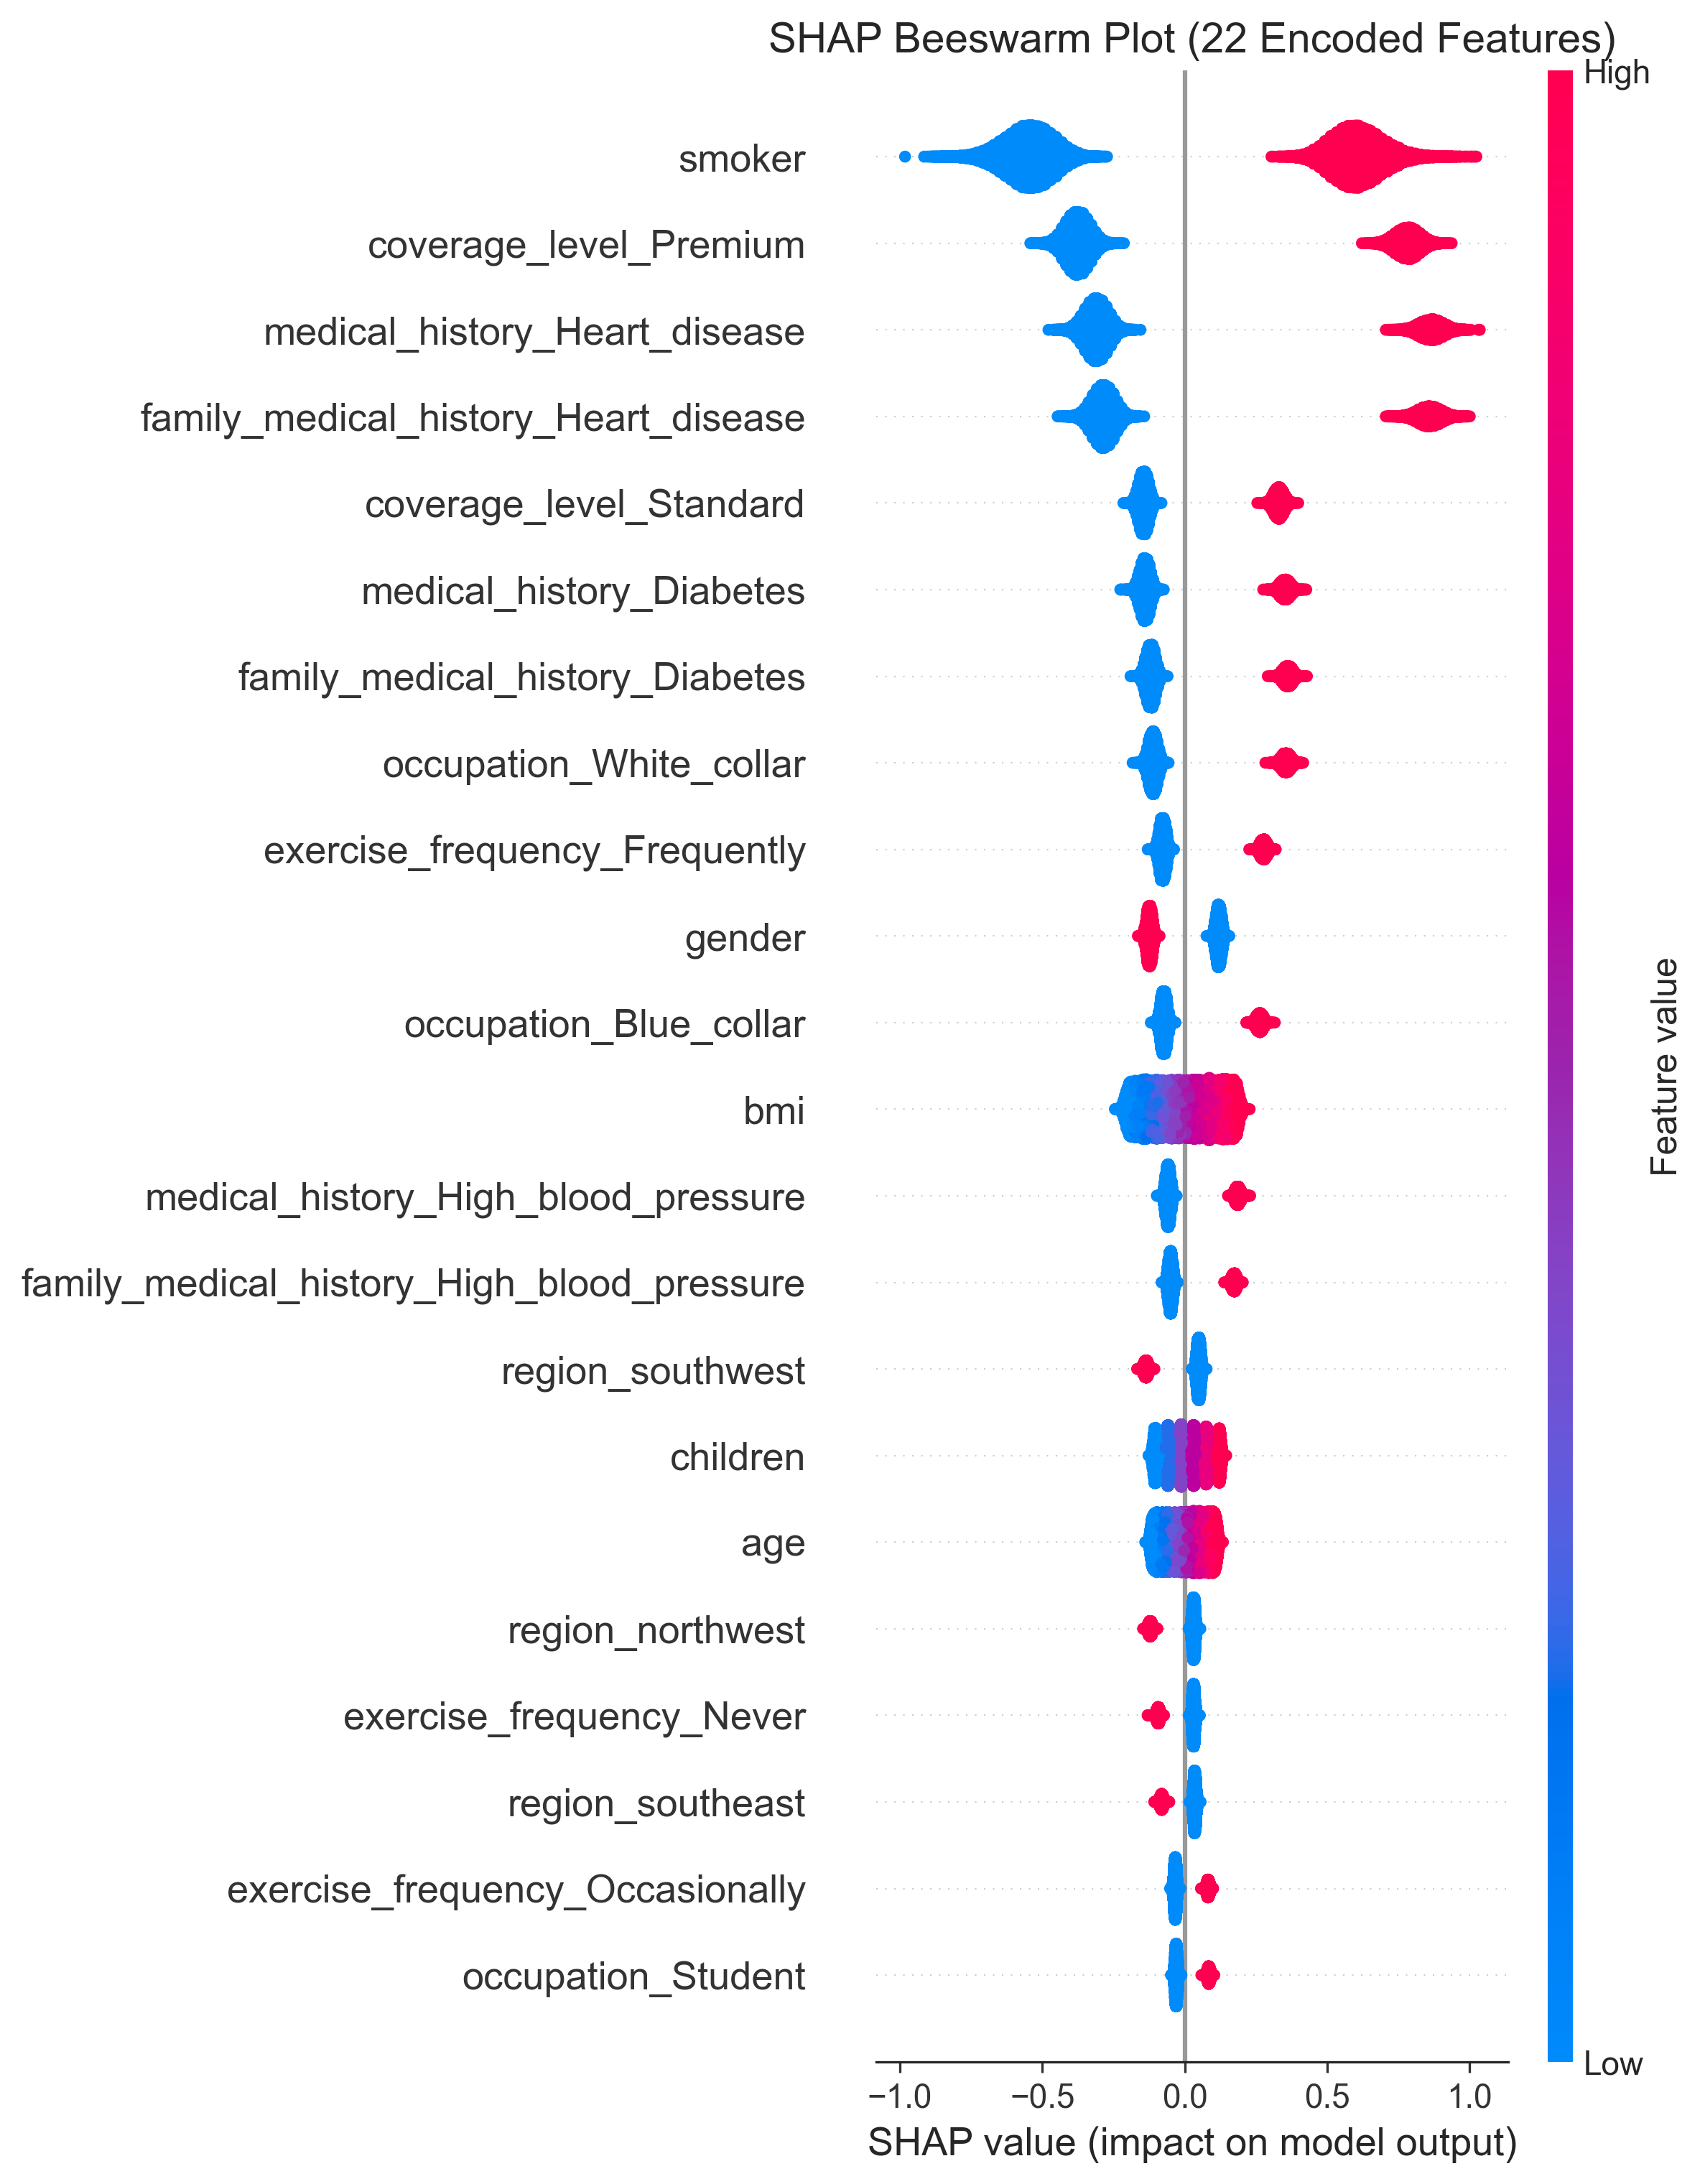
\includegraphics[width=0.72\textwidth]{Thesis/Chapter 4/Figures/fig_shap_beeswarm.png}
\caption{SHAP beeswarm plot for all 22 encoded features.}
\label{fig:shap_beeswarm_ch4}
\end{figure}

\noindent
Figure~\ref{fig:shap_beeswarm_ch4} provides a feature-level view of
the Shapley attributions across all 22 encoded inputs. Several patterns
are visible:

\begin{enumerate}
    \item \textbf{Smoker:} The binary \texttt{smoker} variable produces
    a clear bimodal separation. High feature values (red, smoker $=$ yes)
    yield large positive SHAP values (approximately $+0.5$ to $+1.0$),
    while low feature values (blue, smoker $=$ no) yield large negative
    SHAP values (approximately $-0.5$ to $-0.7$). This confirms that
    smoking status is the single largest determinant of fitted predicted
    costs.

    \item \textbf{Coverage level:} The \texttt{coverage\_level\_Premium}
    dummy exhibits a similar bimodal pattern: premium coverage pushes
    predictions upward ($+0.3$ to $+0.7$), while its absence pulls
    predictions downward. The \texttt{coverage\_level\_Standard} dummy
    shows a complementary pattern of smaller magnitude.

    \item \textbf{Medical and family medical history:} The Heart disease
    dummies for both \texttt{medical\_history} and
    \texttt{family\_medical\_history} produce the next largest
    attributions. High feature values (Heart disease present)
    consistently increase predicted costs by approximately $+0.3$ to
    $+0.8$.

    \item \textbf{Continuous variables:} \texttt{bmi}, \texttt{children}
    and \texttt{age} display more diffuse SHAP distributions centred
    near zero, consistent with their smaller global importance. The
    \texttt{bmi} swarm shows a broad purple-to-pink gradient, reflecting
    its continuous nature, but the individual SHAP magnitudes remain
    small (mostly within $\pm 0.15$).
\end{enumerate}

\subsubsection{Training versus Monte Carlo attribution invariance}

\begin{figure}[H]
\centering
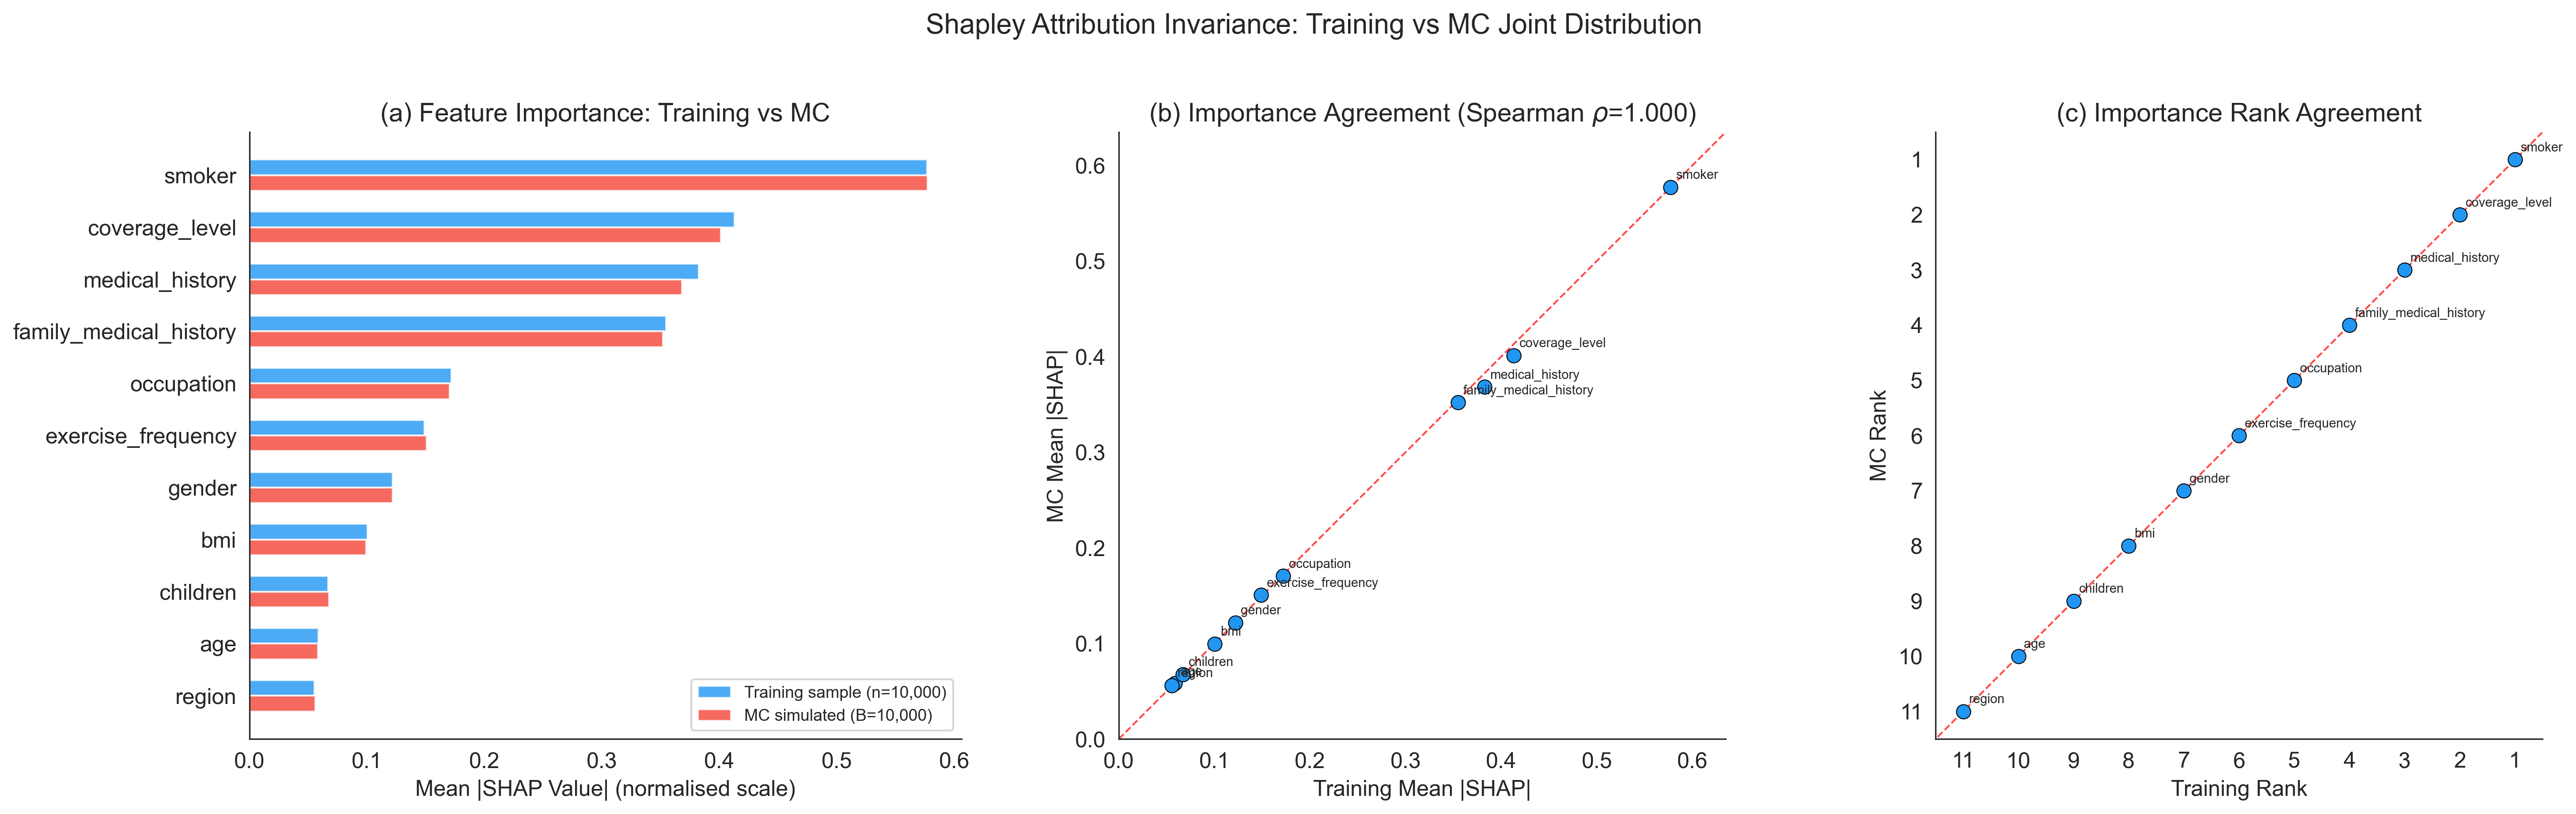
\includegraphics[width=0.95\textwidth]{Thesis/Chapter 4/Figures/fig_shap_training_vs_mc_invariance.png}
\caption{Shapley attribution invariance: training data versus Monte Carlo profiles.}
\label{fig:shap_training_vs_mc_invariance_ch4}
\end{figure}

\noindent
Figure~\ref{fig:shap_training_vs_mc_invariance_ch4} compares the
Shapley attributions computed on the training data with those computed on
the Monte Carlo simulated profiles. The Spearman rank correlation
between the two feature-importance vectors is $\rho_{\mathrm{S}} =
1.000$: all 11 raw variables occupy the same importance rank under both
input regimes. The scatter plot in panel~(b) shows that the mean
$|\text{SHAP}|$ values fall on the diagonal, with no systematic
deviation. This result extends the parametric-versus-bootstrap invariance
finding of Section~\ref{sec:mc_input_validation} (Spearman
$\rho = 0.991$) and confirms that the fitted \gls{dnn}'s internal
feature-importance structure is preserved when evaluated on the Monte
Carlo simulated input space.


% =============================================================
\subsection{High-Cost Conditional Shapley Analysis}
\label{sec:highcost_conditional_results}

The high-cost region was defined using the quantile-based thresholds
$u_{\tau}$ (equation~\eqref{eq:high_cost_threshold}) applied to the
Monte Carlo predicted-cost distribution.
Table~\ref{tab:highcost_thresholds_ch4} reports the three threshold
values and the corresponding high-cost set sizes.

\begin{table}[H]
\centering
\caption{High-cost thresholds from the Monte Carlo predicted-cost
distribution.}
\label{tab:highcost_thresholds_ch4}
\small
\renewcommand{\arraystretch}{1.15}
\begin{tabular}{lrrrr}
\toprule
\textbf{Threshold} & $\boldsymbol{\tau}$ &
$\boldsymbol{u_{\tau}}$ \textbf{(R)} &
$\boldsymbol{|\mathcal{H}_{\tau}|}$ &
\textbf{Proportion} \\
\midrule
$\tau_{90}$ & 0.90 & 22\,482 & 1\,000 & 0.10 \\
$\tau_{95}$ & 0.95 & 24\,154 & 500 & 0.05 \\
$\tau_{99}$ & 0.99 & 27\,160 & 100 & 0.01 \\
\bottomrule
\end{tabular}
\end{table}

\subsubsection{Conditional versus global importance}

Conditional mean absolute Shapley values were computed for profiles in
$\mathcal{H}_{\tau}$ at each threshold and compared with the global
values.

\begin{figure}[H]
\centering
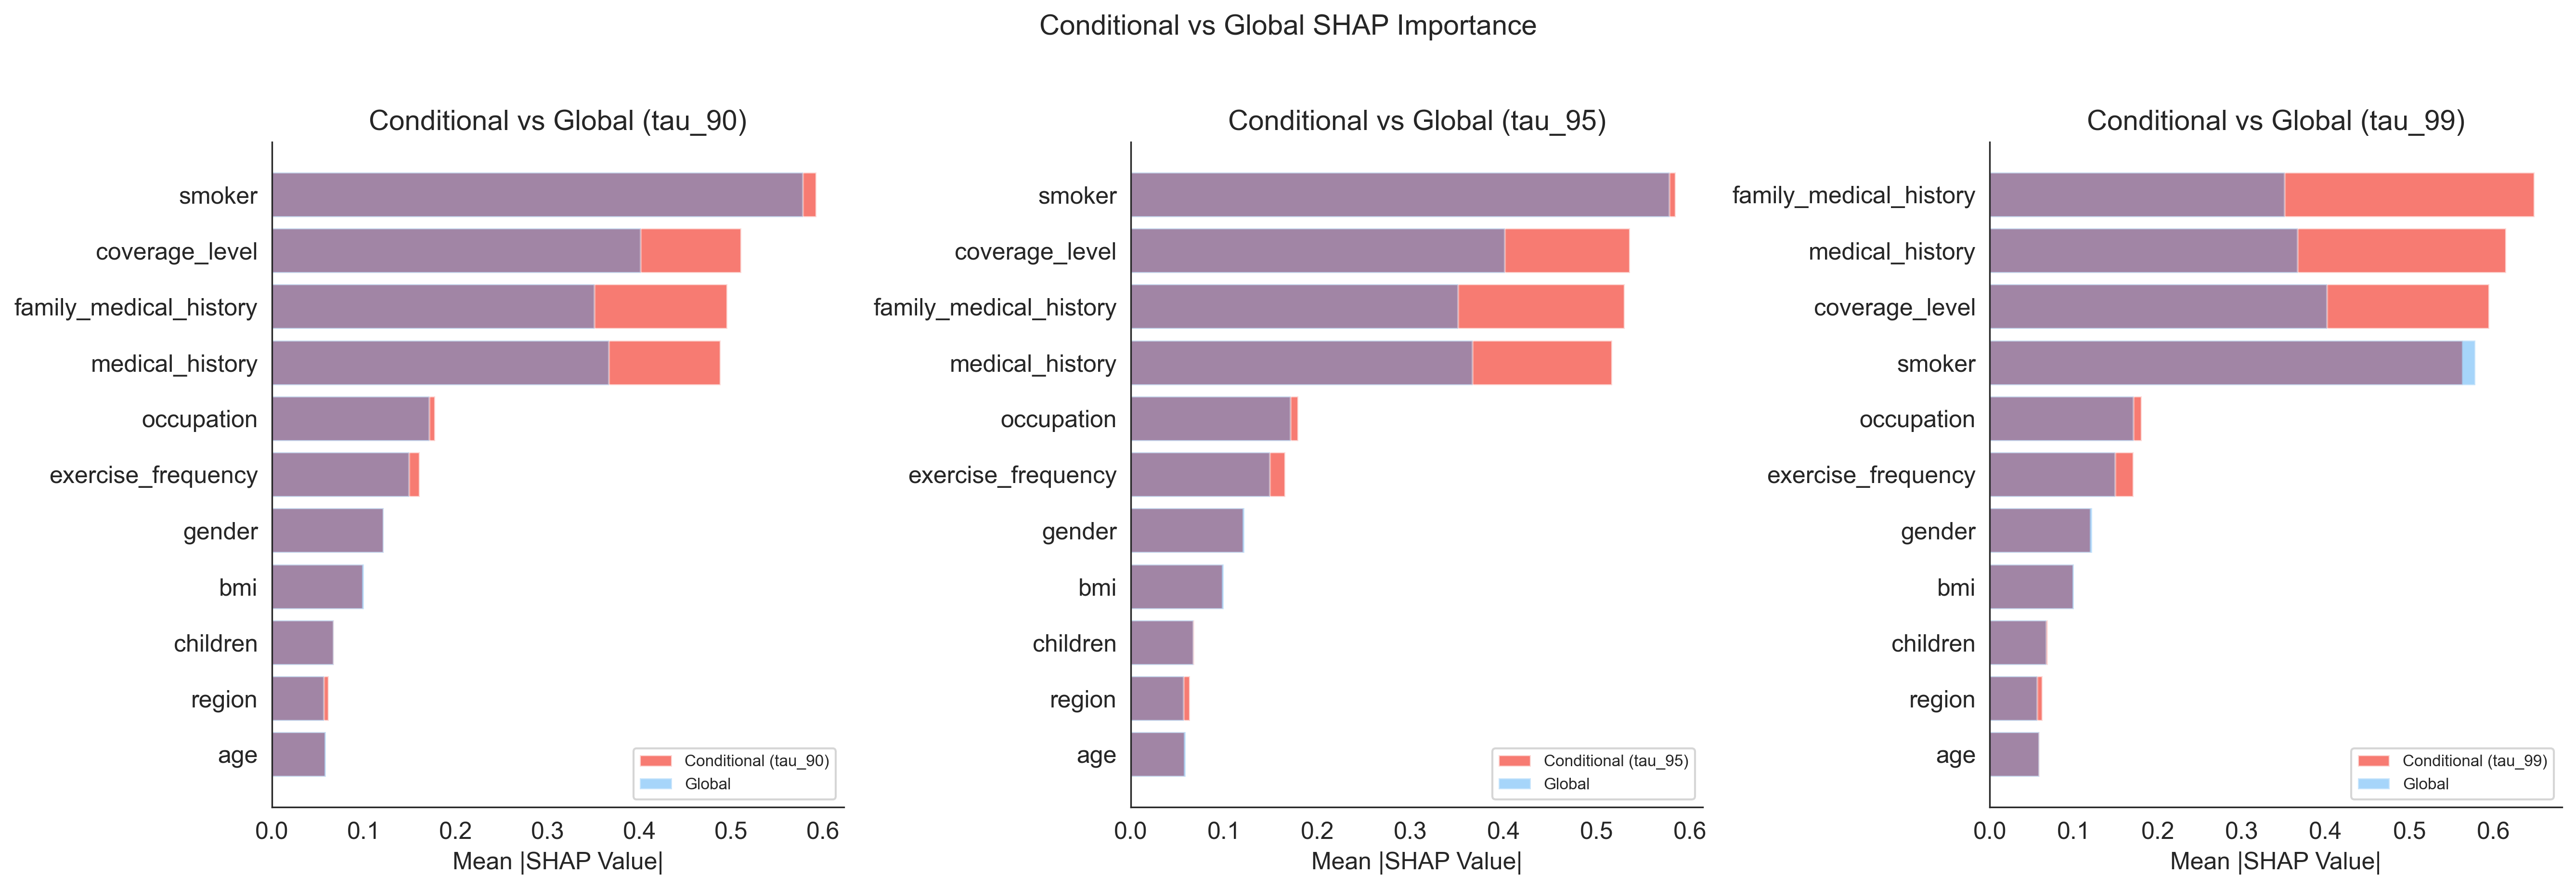
\includegraphics[width=0.95\textwidth]{Thesis/Chapter 4/Figures/fig_shap_conditional_importance.png}
\caption{Conditional versus global mean $|\text{SHAP}|$ importance at three upper-tail thresholds.}
\label{fig:shap_conditional_importance_ch4}
\end{figure}

\noindent
Figure~\ref{fig:shap_conditional_importance_ch4} reveals a progressive
shift in the feature-importance ranking as the threshold moves into the
extreme upper tail:

\begin{itemize}
    \item At $\tau_{90}$, the ranking mirrors the global ordering:
    \texttt{smoker} remains the most important variable, followed by
    \texttt{coverage\_level}, \texttt{medical\_history} and
    \texttt{family\_medical\_history}. The conditional importance values
    are slightly higher than the global values for the top four
    variables, reflecting the more extreme nature of the high-cost
    profiles.

    \item At $\tau_{95}$, the top four variables maintain similar
    positions, but \texttt{family\_medical\_history} and
    \texttt{medical\_history} show increased conditional importance
    relative to their global values.

    \item At $\tau_{99}$, a ranking reversal occurs:
    \texttt{family\_medical\_history} ($I_{g,0.99} = 0.622$) and
    \texttt{medical\_history} ($I_{g,0.99} = 0.608$) overtake
    \texttt{smoker} ($I_{g,0.99} = 0.566$) as the most important
    variables. \texttt{coverage\_level} ($I_{g,0.99} = 0.599$) also
    exceeds \texttt{smoker} in the extreme tail.
\end{itemize}

\noindent
Table~\ref{tab:shap_conditional_values_ch4} reports the conditional
mean $|\text{SHAP}|$ values at all three thresholds alongside the global
values.

\begin{table}[H]
\centering
\caption{Mean absolute Shapley values: global and conditional at each
high-cost threshold (normalised scale).}
\label{tab:shap_conditional_values_ch4}
\small
\renewcommand{\arraystretch}{1.15}
\begin{tabular}{lrrrr}
\toprule
\textbf{Variable} & \textbf{Global} & $\boldsymbol{\tau_{90}}$ &
$\boldsymbol{\tau_{95}}$ & $\boldsymbol{\tau_{99}}$ \\
\midrule
\texttt{smoker} & 0.577 & 0.596 & 0.584 & 0.566 \\
\texttt{coverage\_level} & 0.401 & 0.515 & 0.537 & 0.599 \\
\texttt{medical\_history} & 0.368 & 0.502 & 0.518 & 0.608 \\
\texttt{family\_medical\_history} & 0.352 & 0.498 & 0.531 & 0.622 \\
\texttt{occupation} & 0.170 & 0.183 & 0.185 & 0.178 \\
\texttt{exercise\_frequency} & 0.151 & 0.164 & 0.171 & 0.191 \\
\texttt{gender} & 0.122 & 0.122 & 0.122 & 0.120 \\
\texttt{bmi} & 0.099 & 0.099 & 0.095 & 0.092 \\
\texttt{children} & 0.068 & 0.068 & 0.068 & 0.065 \\
\texttt{age} & 0.058 & 0.058 & 0.057 & 0.057 \\
\texttt{region} & 0.056 & 0.062 & 0.062 & 0.070 \\
\bottomrule
\end{tabular}
\end{table}

\subsubsection{Threshold stability of the importance ranking}

\begin{figure}[H]
\centering
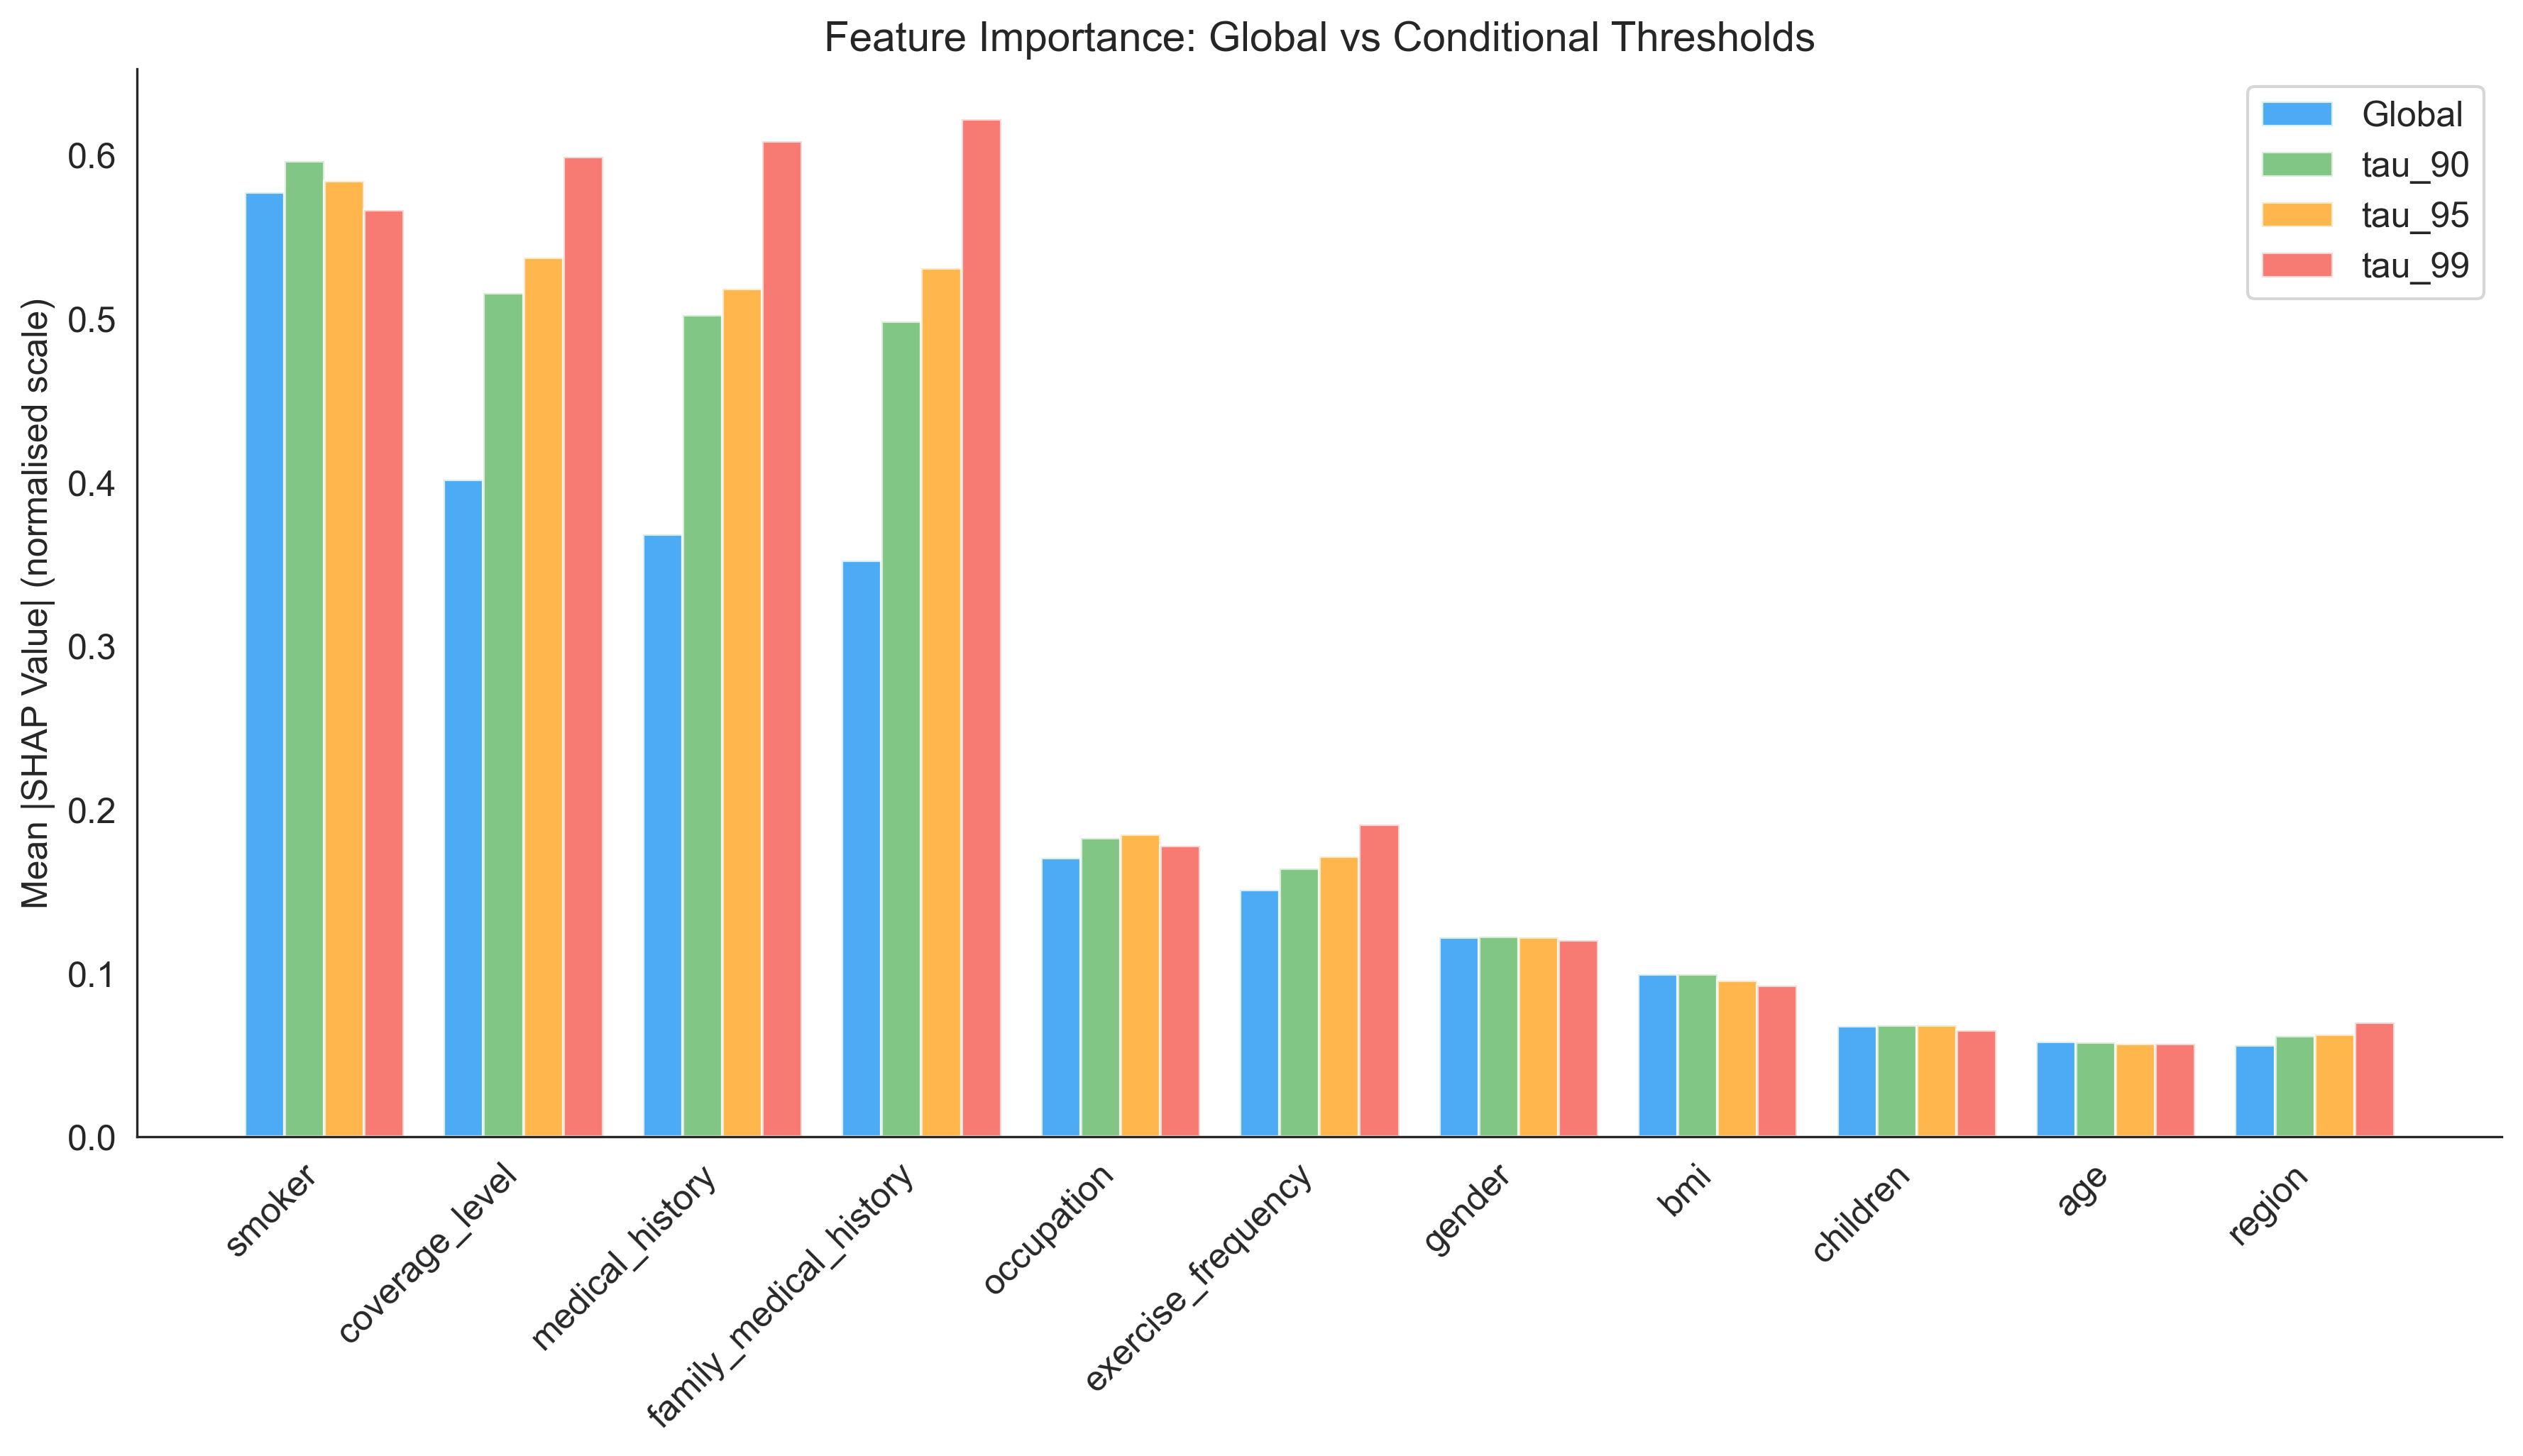
\includegraphics[width=0.85\textwidth]{Thesis/Chapter 4/Figures/fig_shap_threshold_comparison.png}
\caption{Feature importance across thresholds: mean $|\text{SHAP}|$
values at the global, $\tau_{90}$, $\tau_{95}$ and $\tau_{99}$ levels
for all 11 raw variables.}
\label{fig:shap_threshold_comparison_ch4}
\end{figure}

\noindent
Figure~\ref{fig:shap_threshold_comparison_ch4} displays the
threshold-comparison bar chart. The dominant pattern is a monotonic
increase in the conditional importance of
\texttt{coverage\_level}, \texttt{medical\_history} and
\texttt{family\_medical\_history} as the threshold moves from the global
level through $\tau_{90}$ and $\tau_{95}$ to $\tau_{99}$. In contrast,
\texttt{smoker} shows a slight decline in conditional importance at the
most extreme threshold ($0.566$ at $\tau_{99}$ versus $0.577$ globally).
This decline does not indicate that smoking status becomes
unimportant; rather, it reflects a ceiling effect: nearly all profiles
in the extreme upper tail are smokers (as confirmed in
Figure~\ref{fig:highcost_profiles_ch4} below), so the binary variable
contributes a near-constant positive attribution with reduced
variability, while the remaining features differentiate among the
high-cost profiles.

The second tier of variables (\texttt{occupation},
\texttt{exercise\_frequency}, \texttt{gender}, \texttt{bmi},
\texttt{children}, \texttt{age} and \texttt{region}) remains stable
across all thresholds, with conditional importance values close to
their global values. This stability indicates that these variables
contribute a consistent baseline attribution regardless of the cost
region.

The ranking reversal at $\tau_{99}$ directly addresses the research gap
identified in Section~\ref{sec:research_gap}: existing health-cost
prediction studies typically report global feature importance on observed
data only \citep{kaushik2022machine, rozemberczki2022shapley}, without
conditioning attributions on specific regions of the predicted-cost
distribution.  The conditional Shapley analysis demonstrates that global
importance rankings can be misleading when the interest lies in the
upper tail, because a variable that dominates on average (smoking status)
may lose its discriminating power within an extreme subpopulation where
it is nearly constant.  This distinction has not been documented in the
health insurance cost-prediction literature reviewed in
Chapter~\ref{sec:literature_review}.

\subsubsection{High-cost profile characteristics}

\begin{figure}[H]
\centering
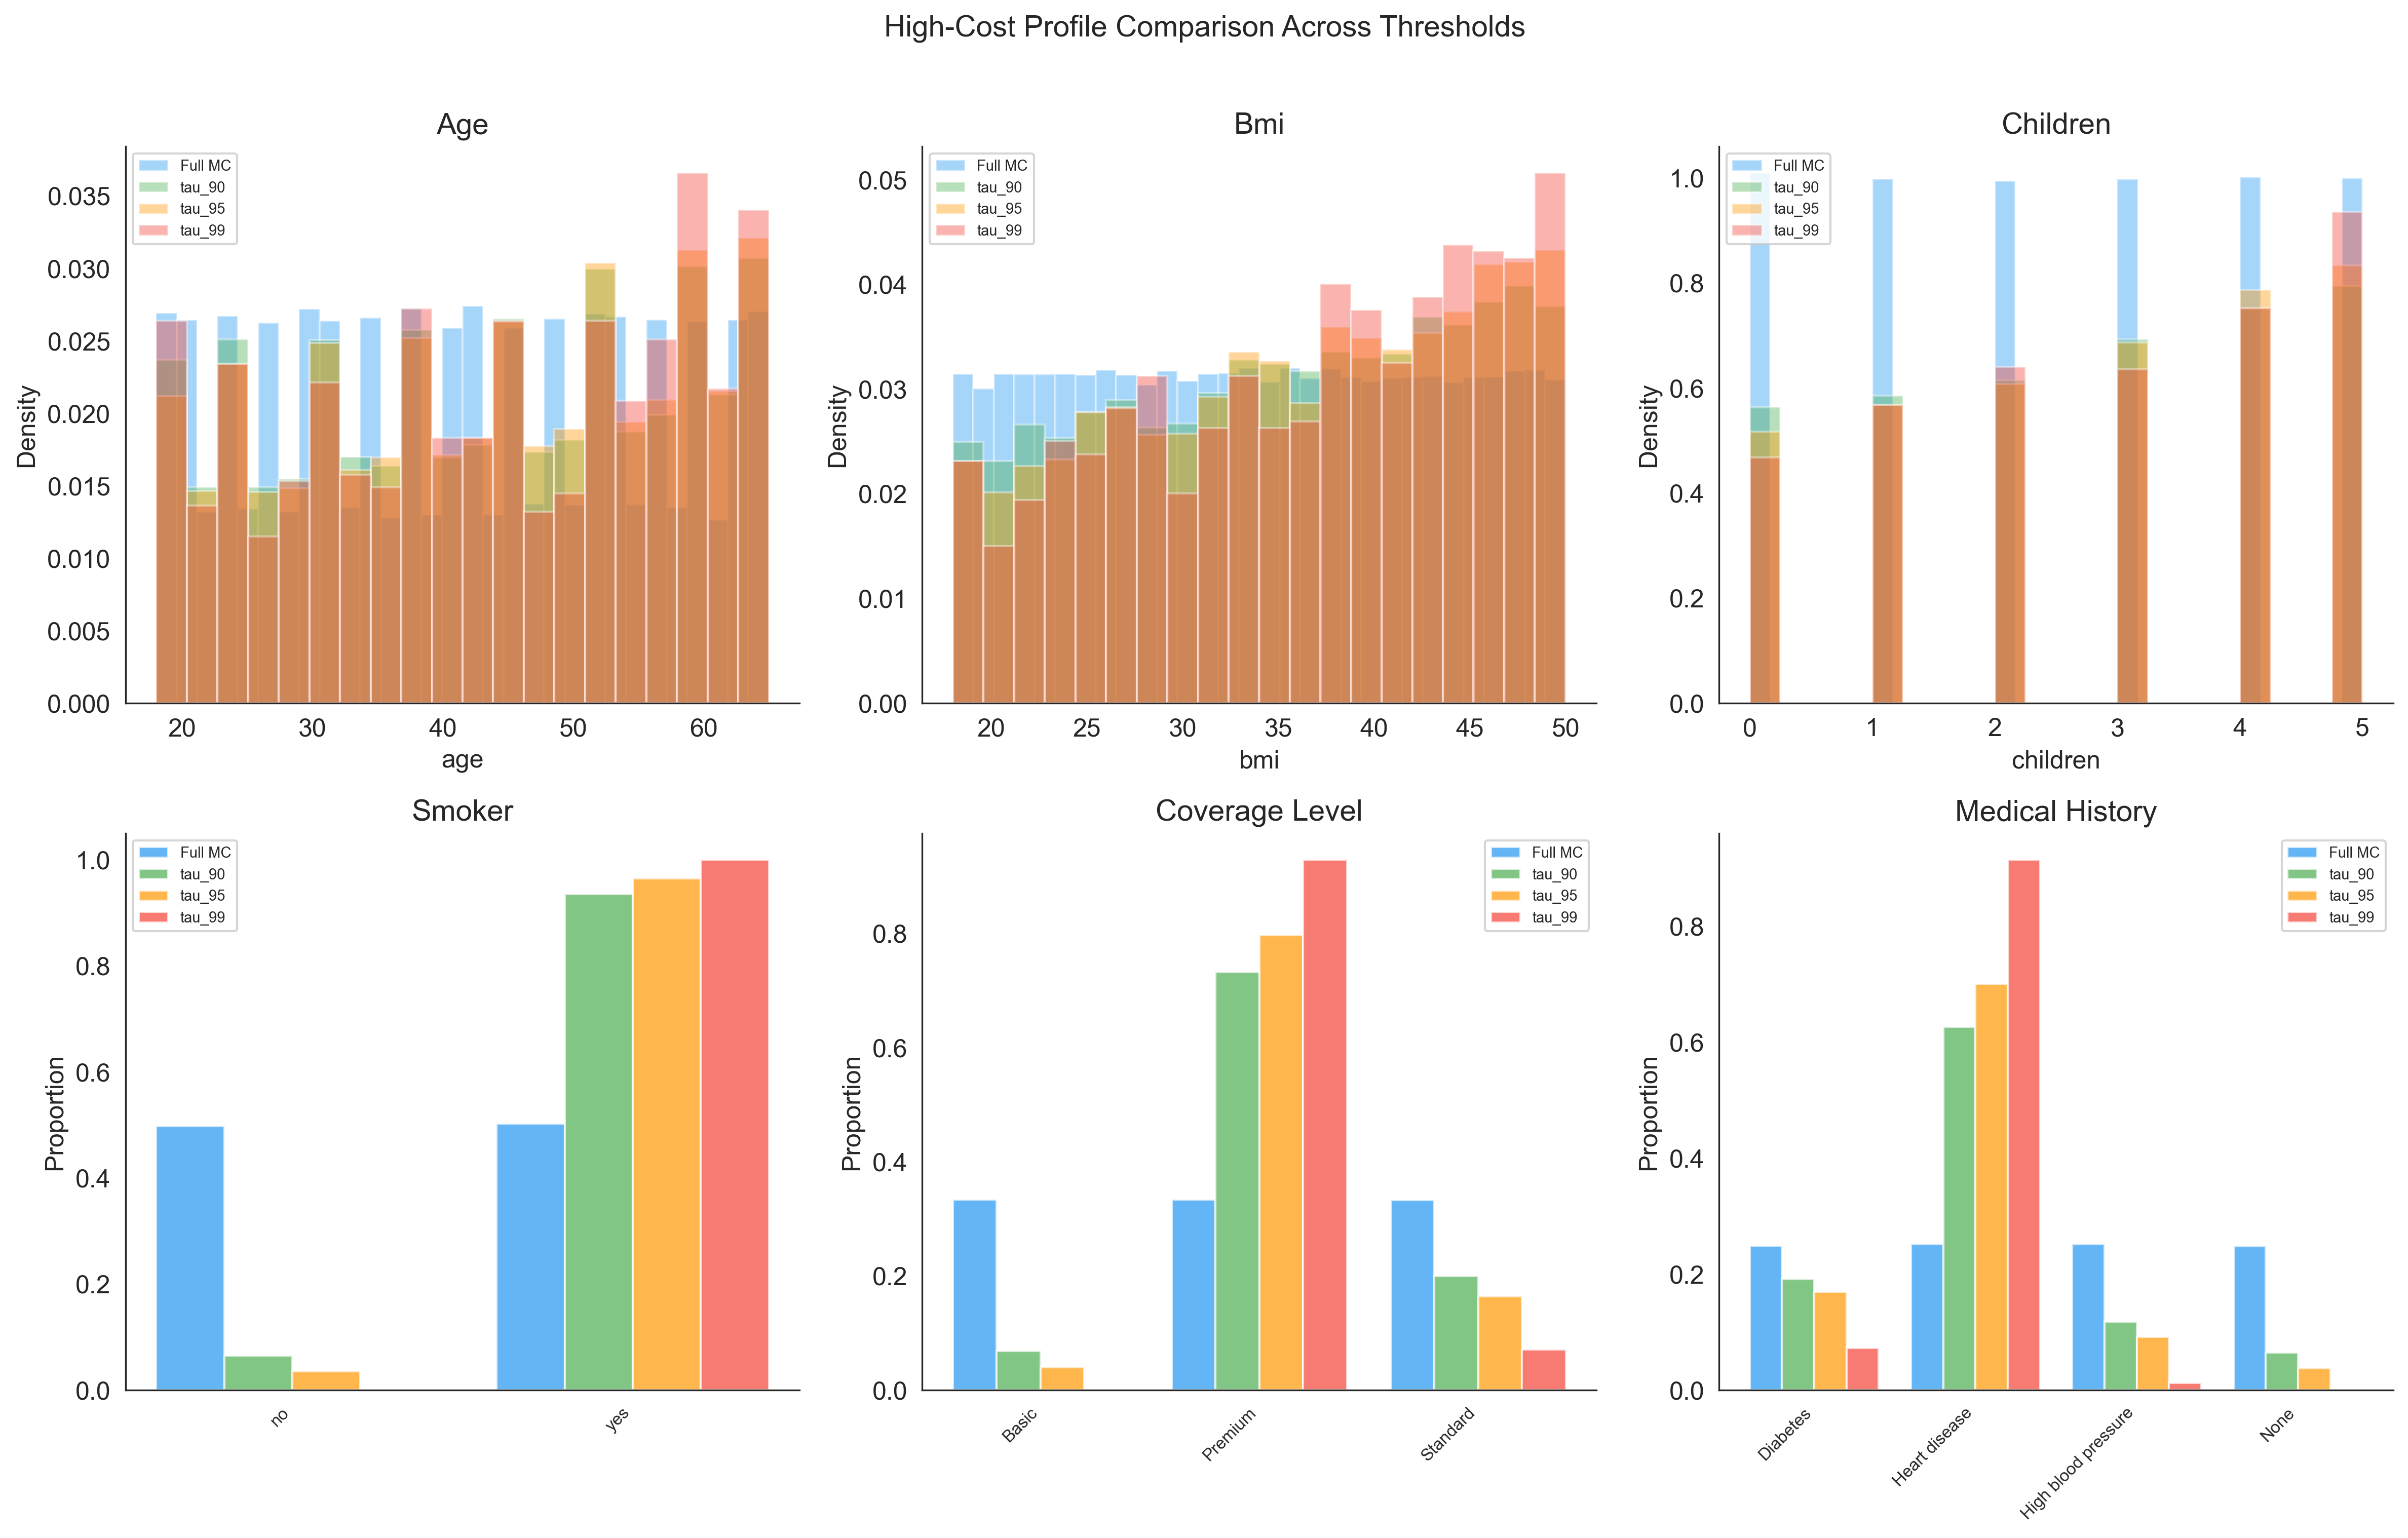
\includegraphics[width=0.95\textwidth]{Thesis/Chapter 4/Figures/fig_highcost_profile_comparison.png}
\caption{Distributional profiles of the high-cost sets compared with the full Monte Carlo sample.}
\label{fig:highcost_profiles_ch4}
\end{figure}

\noindent
Figure~\ref{fig:highcost_profiles_ch4} profiles the composition of the
high-cost sets at each threshold. The categorical panels reveal a
progressive concentration:

\begin{itemize}
    \item \textbf{Smoker:} The proportion of smokers increases from
    approximately $50\%$ in the full Monte Carlo sample to approximately
    $93\%$ at $\tau_{90}$, $96\%$ at $\tau_{95}$ and $99\%$ at
    $\tau_{99}$. At the most extreme threshold, virtually all high-cost
    profiles are smokers.

    \item \textbf{Coverage level:} The proportion of Premium-tier
    policyholders rises from approximately $33\%$ (full MC) to $75\%$
    at $\tau_{90}$, $80\%$ at $\tau_{95}$ and approximately $90\%$ at
    $\tau_{99}$. Basic-tier policyholders are nearly absent from the
    extreme tail.

    \item \textbf{Medical history:} Heart disease dominates the
    high-cost sets: its proportion increases from approximately $25\%$
    (full MC) to $68\%$ at $\tau_{90}$, $77\%$ at $\tau_{95}$ and
    approximately $85\%$ at $\tau_{99}$. Profiles with no medical
    history condition are progressively excluded from the upper tail.
\end{itemize}

\noindent
The continuous variables (\texttt{age}, \texttt{bmi},
\texttt{children}) show little change in their distributional shapes
across thresholds, consistent with their small and stable conditional
Shapley values. This confirms that the high-cost region is defined
primarily by the categorical risk factors rather than the continuous
covariates.

\subsubsection{Representative high-cost waterfall decomposition}

\begin{figure}[H]
\centering
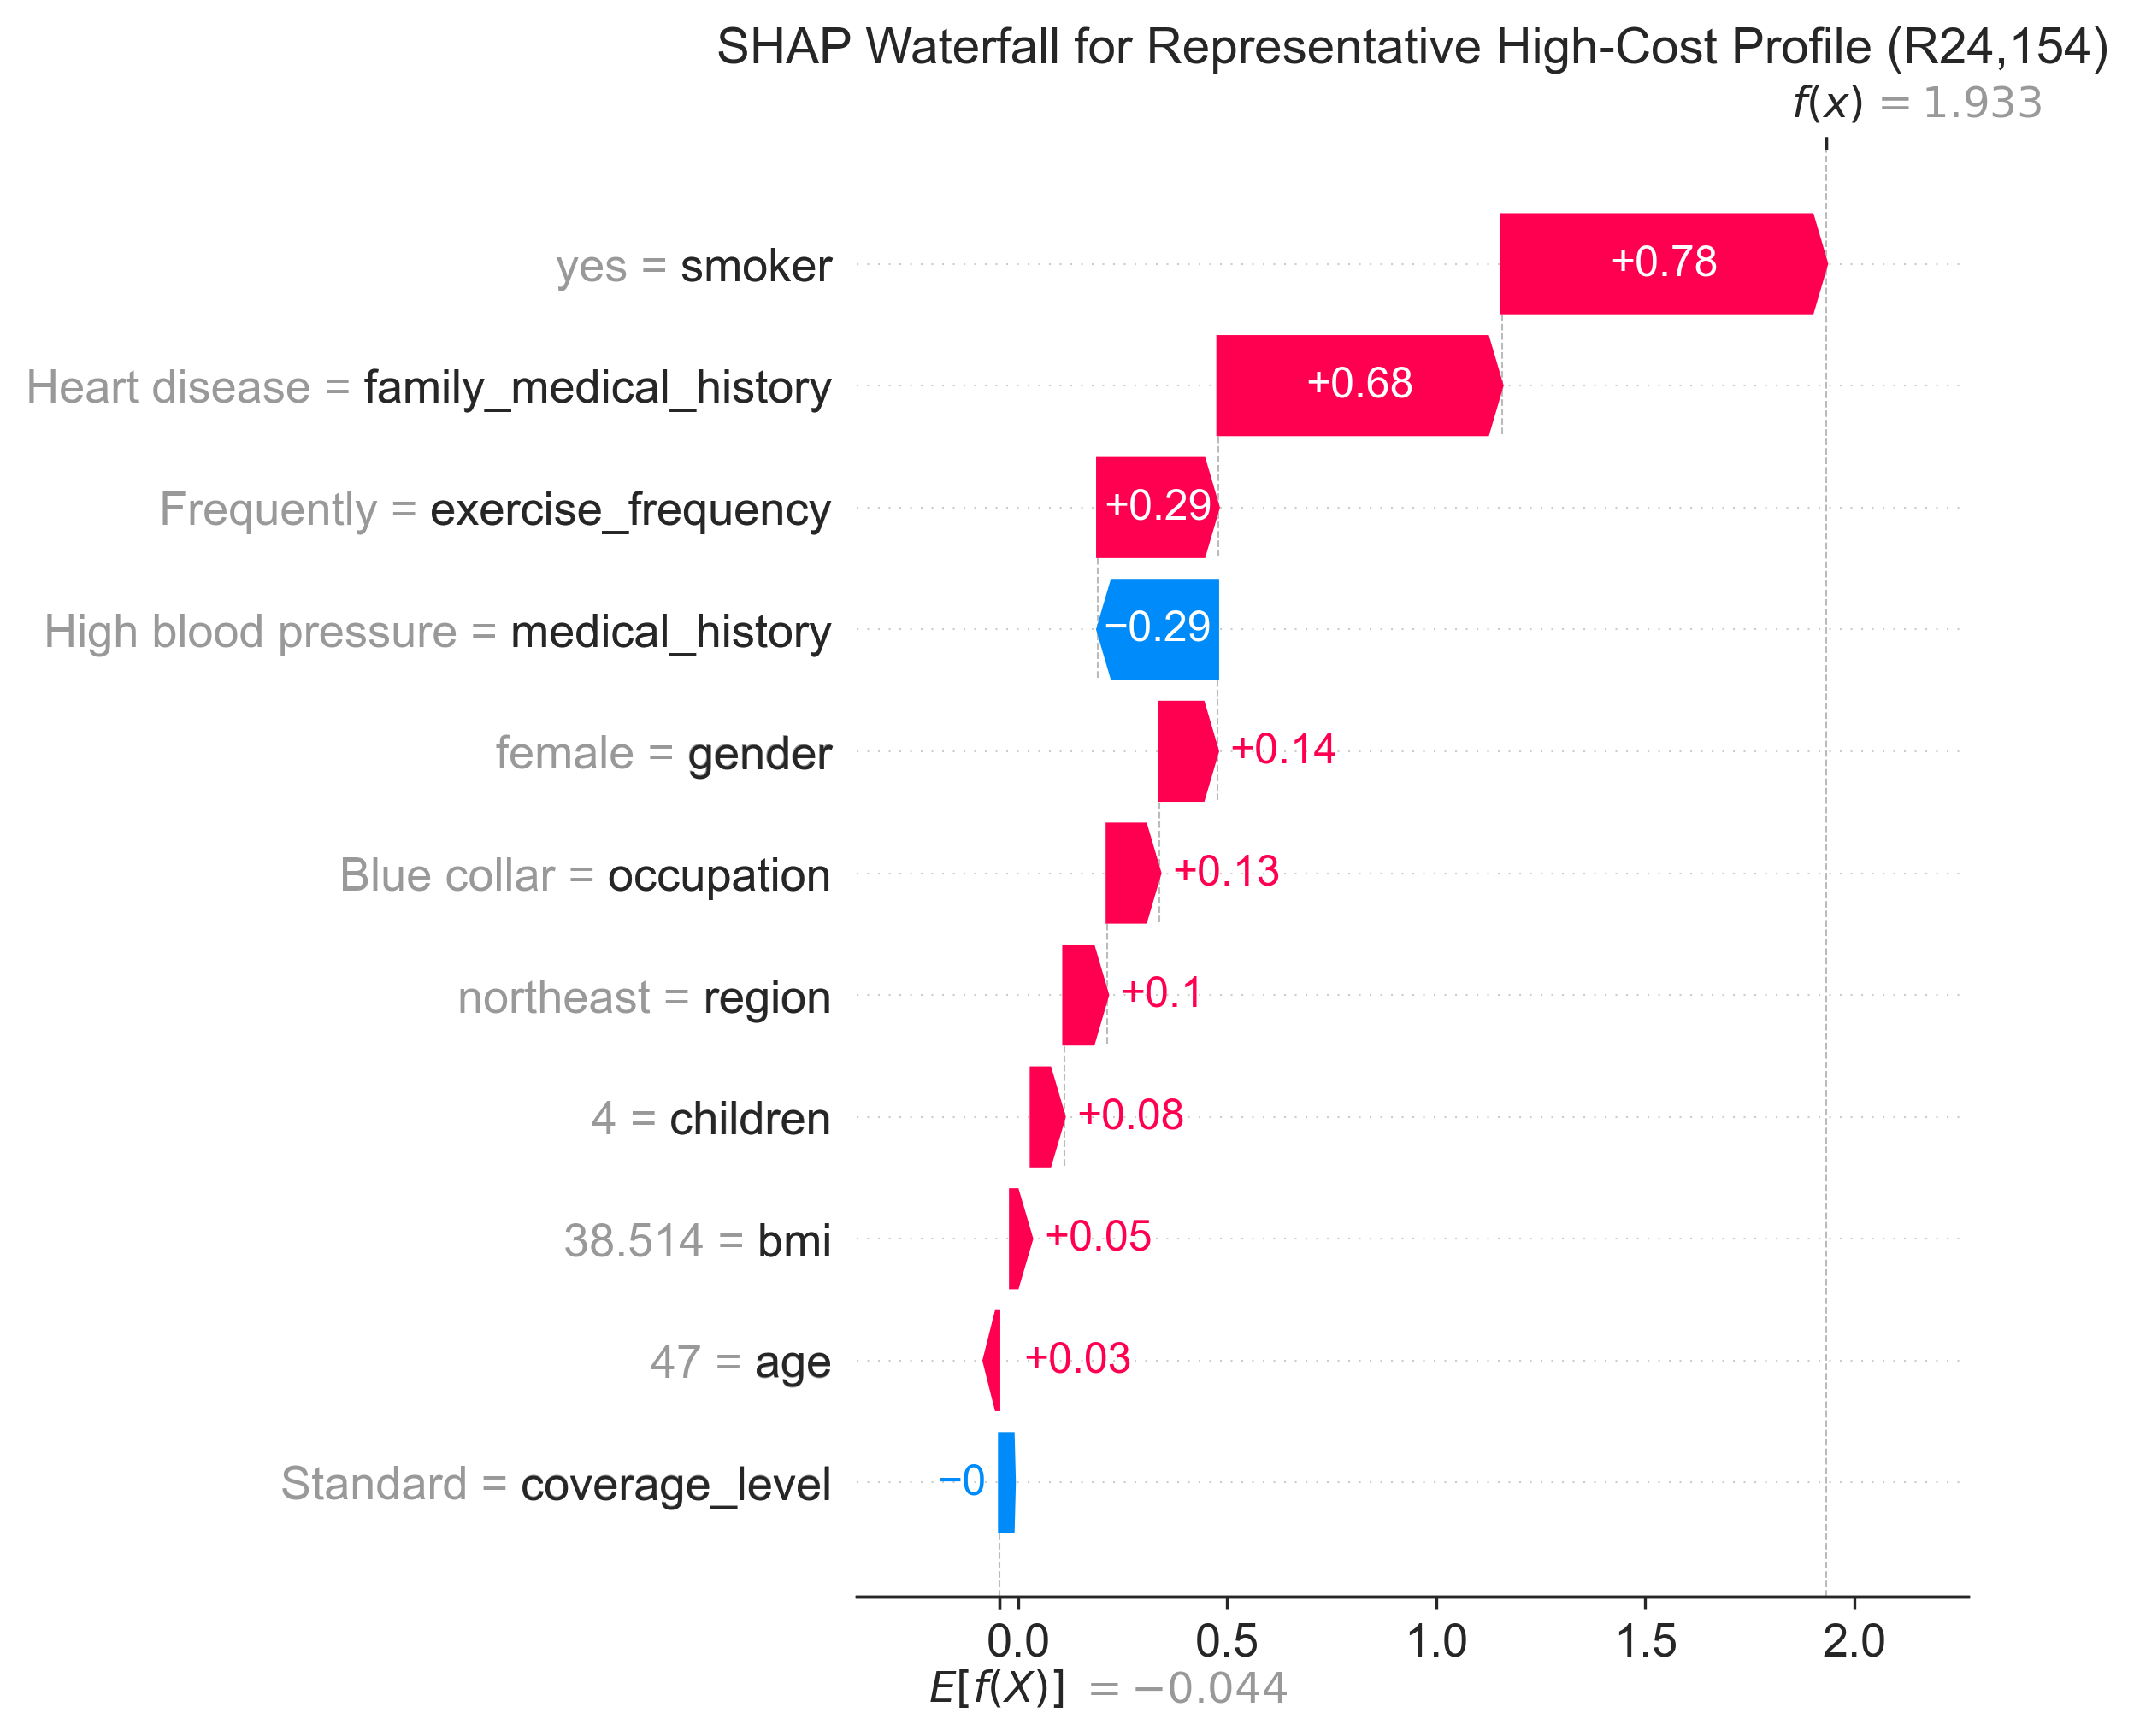
\includegraphics[width=0.75\textwidth]{Thesis/Chapter 4/Figures/fig_shap_highcost_waterfall.png}
\caption{SHAP waterfall plot for a representative high-cost profile
at the $\tau_{95}$ threshold (predicted cost R24\,154).}
\label{fig:shap_waterfall_ch4}
\end{figure}

\noindent
Figure~\ref{fig:shap_waterfall_ch4} decomposes a representative
high-cost profile at the $\tau_{95}$ threshold. The profile has the
following characteristics: age~$= 47$, \texttt{bmi}~$= 38.5$,
\texttt{children}~$= 4$, \texttt{smoker}~$=$ yes,
\texttt{family\_medical\_history}~$=$ Heart disease,
\texttt{exercise\_frequency}~$=$ Frequently,
\texttt{medical\_history}~$=$ High blood pressure,
\texttt{gender}~$=$ female, \texttt{occupation}~$=$ Blue collar,
\texttt{region}~$=$ northeast,
\texttt{coverage\_level}~$=$ Standard.

The waterfall decomposition shows that the prediction is driven upward
from the baseline ($E[f(X)] = -0.044$) to the final prediction
($f(x) = 1.933$) primarily by three variables:
\texttt{smoker} ($+0.78$), \texttt{family\_medical\_history} ($+0.68$)
and \texttt{exercise\_frequency} ($+0.29$). A negative contribution
from \texttt{medical\_history} ($-0.29$) partially offsets these
positive effects, reflecting that High blood pressure carries a lower
attribution than Heart disease within the \texttt{medical\_history}
variable. The remaining variables contribute small positive amounts,
with \texttt{coverage\_level} contributing nearly zero ($-0.00$) because
the Standard tier occupies a middle position in the coverage hierarchy.

This waterfall illustrates the additive decomposition guaranteed by the
Shapley efficiency axiom: the contributions sum exactly to the
difference between the prediction and the baseline, as required by
equation~\eqref{eq:shapley_decomp}.


% =============================================================
\subsection{Integration of Monte Carlo and Shapley Results}
\label{sec:mc_shapley_integration}

The Monte Carlo and Shapley analyses provide complementary perspectives
on the fitted \gls{dnn}'s behaviour. The Monte Carlo simulation
identifies the distributional regions of interest within the
predicted-cost landscape, while the Shapley-value decomposition reveals
which input variables are associated with those regions.

The Monte Carlo predicted-cost distribution
(Figure~\ref{fig:mc_predicted_cost_distribution_ch4}) is approximately
symmetric with a mean of R16\,707 and an upper tail extending to
R31\,466. Within this landscape, three quantile-based thresholds
define high-cost regions of increasing severity:
$u_{0.90} = \text{R22\,482}$, $u_{0.95} = \text{R24\,154}$ and
$u_{0.99} = \text{R27\,160}$.

The global Shapley analysis
(Figure~\ref{fig:shap_global_importance_ch4}) identifies
\texttt{smoker} as the dominant driver of fitted predictions across
the full simulated input space. However, the conditional analysis
(Figures~\ref{fig:shap_conditional_importance_ch4}
and~\ref{fig:shap_threshold_comparison_ch4}) reveals that the
attribution structure changes in the upper tail. As the high-cost
threshold becomes more stringent, the conditional importance of
\texttt{coverage\_level}, \texttt{medical\_history} and
\texttt{family\_medical\_history} increases monotonically, while the
importance of \texttt{smoker} declines slightly.

The profile-level analysis
(Figure~\ref{fig:highcost_profiles_ch4}) explains this
re-ordering: at $\tau_{99}$, virtually all high-cost profiles are
smokers ($99\%$), so smoking status no longer differentiates among
profiles within the extreme tail. The variables that differentiate
high-cost profiles from one another are therefore coverage tier,
personal medical history and family medical history. At $\tau_{99}$,
approximately $90\%$ of high-cost profiles hold Premium coverage and
$85\%$ report Heart disease. These three variables collectively define
the archetype of the extreme upper-tail profile.

The continuous covariates (\texttt{age}, \texttt{bmi},
\texttt{children}) play a limited role at all threshold levels. Their
conditional importance values remain close to their global values, and
their distributional shapes within the high-cost sets are not
meaningfully different from those in the full Monte Carlo sample. The
fitted \gls{dnn} therefore assigns the dominant cost-driving role to
the categorical risk factors, with the continuous variables contributing
a modest, stable baseline effect.

The invariance checks reinforce the robustness of these findings. The
Shapley attributions are stable whether computed on training data or
Monte Carlo profiles (Spearman $\rho = 1.000$,
Figure~\ref{fig:shap_training_vs_mc_invariance_ch4}), and the
residual-augmented sensitivity analysis
(Figure~\ref{fig:mc_residual_augmented_ch4}) confirms that the
predicted-cost distribution is not sensitive to fitted residual
variability. The attribution patterns therefore reflect the fitted
model's learned internal structure rather than artefacts of the input
regime or residual noise.

These results are summarised, evaluated and situated within the broader
context of the study in Chapter~\ref{sec:conclusion}.


% =============================================================
% Chapter 5: Conclusion
% =============================================================
\clearpage
% =============================================================
% CHAPTER 5 : CONCLUSION
% =============================================================

\section{Conclusion}
\label{sec:conclusion}

% ---------------------------------------------------------
% 5.1 SUMMARY OF FINDINGS
% ---------------------------------------------------------

\subsection{Summary of Findings}
\label{sec:summary_of_findings}

This dissertation developed and applied a three-stage statistical
framework for health insurance cost prediction, combining deep neural
network regression, parametric Monte Carlo simulation and Shapley-value
attribution within a single empirical workflow.  The analysis was
conducted on a publicly available Kaggle benchmark dataset containing one
million policyholder records with eleven predictor variables and a
continuous monetary response.

The predictive stage demonstrated that a feed-forward deep neural network
with a funnel architecture, CELU activation and Nadam optimisation
achieves strong out-of-sample performance on the benchmark data, with
test-set $R^2 = 0.9957$, MAE $= \text{R}251$ and RMSE $= \text{R}290$.
A five-phase sequential hyperparameter comparison identified this
configuration from among 16 candidate settings.  A baseline comparison
with a Gamma generalised linear model (log-link) confirmed that the
\gls{dnn} substantially outperforms the actuarial-standard model class on
this dataset, reducing the test RMSE by $68.2\%$ and the test MAE by
$59.8\%$ relative to the \gls{glm}.  The near-identical training and test
performance metrics for both models ruled out overfitting, and the
data-leakage prevention protocols described in
Section~\ref{sec:data_leakage_prevention} ensured that all reported
metrics reflect genuine out-of-sample predictive ability.

The simulation stage generated $B = 10\,000$ synthetic policyholder
profiles from fitted parametric marginal distributions and propagated them
through the trained network to produce a model-implied predicted-cost
distribution centred at R16\,707 with moderate dispersion
(SD $=$ R4\,409) and a mildly right-skewed shape.  Convergence diagnostics
confirmed adequate Monte Carlo precision, and joint-distribution validation
(including an energy distance permutation test, $p = 0.730$) established
that the independent-marginal sampling does not introduce material
distributional distortion.  The residual-augmented sensitivity analysis
confirmed that these findings are robust to fitted residual perturbation.

The explanation stage computed gradient-based Shapley values for all
simulated profiles and summarised feature importance at both the global
and conditional levels.  At the global level, smoking status is the
dominant contributor to predicted cost ($I_g = 0.577$), followed by
coverage level ($0.401$), medical history ($0.368$) and family medical
history ($0.352$).  The conditional analysis at three upper-tail
thresholds ($\tau_{90}$, $\tau_{95}$, $\tau_{99}$) revealed a progressive
shift in the feature-importance ranking.  At $\tau_{99}$, family medical
history ($I_{g,0.99} = 0.622$), medical history ($0.608$) and coverage
level ($0.599$) overtake smoking status ($0.566$) as the most important
variables.  This reversal occurs because smoking status is near-universal
($99\%$) in the extreme tail and therefore loses its discriminating power;
the residual variation among the costliest profiles is instead explained by
coverage tier, medical history and family medical history.  A Shapley
attribution invariance check confirmed that these rankings are consistent
across training-data and Monte Carlo input regimes.

% ---------------------------------------------------------
% 5.2 CONTRIBUTIONS
% ---------------------------------------------------------

\subsection{Contributions}
\label{sec:contributions}

The dissertation makes the following contributions:

\begin{enumerate}
    \item \textbf{Integrated workflow.}  The study presents prediction,
          simulation and explanation as a single, reproducible pipeline
          rather than as isolated modelling exercises.  The integration
          allows the Monte Carlo distribution to define the regions of
          interest for the Shapley analysis, and the Shapley analysis to
          decompose the model behaviour within those regions.

    \item \textbf{Conditional Shapley analysis in the upper tail.}  The
          conditional feature-importance summaries at high-cost thresholds
          demonstrate that the variables driving extreme predicted costs
          differ from those that are most important on average.  This
          finding is relevant to actuarial practice, where understanding
          the drivers of high-cost claims is of particular interest.

    \item \textbf{Model-implied distribution under an explicit input law.}
          The Monte Carlo component constructs a model-implied
          predicted-cost distribution from a formally stated input
          distribution, rather than reporting predictions only at observed
          data points.  This connects the neural network prediction
          function to the simulation-based inference tradition within
          mathematical statistics.

    \item \textbf{Comprehensive validation.}  The dissertation includes
          joint-distribution diagnostics, convergence monitoring,
          residual-augmented sensitivity analysis and Shapley attribution
          invariance checks that go beyond standard predictive-performance
          reporting.

    \item \textbf{GLM benchmark contextualisation.}  The Gamma/log-link
          \gls{glm} comparison contextualises the \gls{dnn}'s performance
          within the actuarial modelling landscape and establishes that the
          predictive superiority reflects genuine model-class advantages
          rather than artefacts of the benchmark data.
\end{enumerate}

% ---------------------------------------------------------
% 5.3 STRENGTHS OF THE STUDY
% ---------------------------------------------------------

\subsection{Strengths of the Study}
\label{sec:strengths}

The study has the following methodological strengths:

\begin{enumerate}
    \item \textbf{Large benchmark dataset.}  The analysis is based on one
          million policyholder records, which provides a substantial sample
          for training, validation and testing.  The training partition
          alone contains $524\,288$ observations, reducing sampling
          variability in model fitting and Shapley-value estimation.

    \item \textbf{Systematic hyperparameter selection.}  The five-phase
          sequential comparison provides a transparent, reproducible method
          for selecting the network configuration.  Each phase is
          documented with validation-loss curves and selection criteria,
          allowing the choices to be scrutinised and replicated.

    \item \textbf{Rigorous validation pipeline.}  The data-leakage
          prevention protocols (Section~\ref{sec:data_leakage_prevention}),
          the joint-distribution input validation, the convergence
          diagnostics and the residual-augmented sensitivity analysis
          collectively establish that the Monte Carlo and Shapley results
          are not artefacts of data contamination, distributional
          mismatch or residual instability.

    \item \textbf{Multi-level attribution analysis.}  The Shapley-value
          analysis is conducted at both the global and conditional levels,
          with three upper-tail thresholds providing a graded view of how
          feature importance evolves into the extreme tail.  The attribution
          invariance check further validates the stability of the results
          across input regimes.

    \item \textbf{Transparent interpretive boundaries.}  All conclusions
          are explicitly qualified as internal to the fitted model and
          benchmark data.  No causal claims are made, and the modelling
          assumptions are stated formally in a consolidated table
          (Table~\ref{tab:modelling_assumptions_ch3}).
\end{enumerate}

% ---------------------------------------------------------
% 5.4 LIMITATIONS
% ---------------------------------------------------------

\subsection{Limitations}
\label{sec:limitations_conclusion}

The following limitations qualify the scope of the findings:

\begin{enumerate}
    \item \textbf{Benchmark data.}  All results are conditional on the
          Kaggle \textit{Insurance Data for Machine Learning} benchmark
          dataset, which has a strong simulated structure.  The unusually
          high predictive performance ($R^2 = 0.9957$) reflects this
          structure and should not be extrapolated to real-world insurance
          portfolios, where data are noisier and relationships between
          covariates and costs are more complex.

    \item \textbf{Limited model comparison.}  The study compares the
          \gls{dnn} against a single classical baseline (Gamma \gls{glm}
          with log-link).  Tree-based models such as random forests and
          gradient-boosted trees, ensemble methods and Bayesian
          alternatives were not evaluated.  A broader model-selection study
          would strengthen the case for the \gls{dnn} as the preferred
          prediction surface.

    \item \textbf{Single fitted network.}  The Monte Carlo and Shapley
          analyses are conditional on a single trained network with a
          fixed random seed.  Variability across random initialisations
          was not quantified.

    \item \textbf{Independent marginals.}  The Monte Carlo input
          distribution is constructed as a product of independent
          marginals.  While the joint-distribution validation confirmed
          that the training-data dependence structure is weak, the
          independence assumption broadens the simulated input space beyond
          what would be observed in practice.

    \item \textbf{Approximate Shapley values.}  The reported attributions
          are gradient-based SHAP approximations, not exact game-theoretic
          Shapley values.  They are conditional on the fitted network, the
          background sample of $m_0 = 200$ observations and the explainer
          settings.

    \item \textbf{Small $\tau_{99}$ sample.}  The conditional Shapley
          summaries at the 99th percentile threshold rely on approximately
          100 simulated profiles.  The ranking reversal observed at
          $\tau_{99}$ is consistent with the monotonic trends at
          $\tau_{90}$ and $\tau_{95}$, but its precision could be improved
          with larger simulation sizes or bootstrap confidence intervals.

    \item \textbf{No causal inference.}  The Shapley decomposition
          identifies variables to which the fitted model assigns large
          contributions.  It does not establish causal relationships
          between input variables and healthcare expenditure.
\end{enumerate}

% ---------------------------------------------------------
% 5.5 RECOMMENDATIONS FOR FUTURE RESEARCH
% ---------------------------------------------------------

\subsection{Recommendations for Future Research}
\label{sec:future_research}

Several directions could extend the framework developed in this
dissertation:

\begin{enumerate}
    \item \textbf{Broader model comparison.}  Future work could extend
          the baseline comparison to include tree-based ensembles (random
          forests, XGBoost, LightGBM) and Bayesian neural networks.  Such
          comparisons would clarify whether the \gls{dnn}'s predictive
          advantage over the \gls{glm} extends to other flexible model
          classes, and whether the Shapley attribution patterns are
          model-dependent or model-invariant.

    \item \textbf{Copula-based Monte Carlo inputs.}  Replacing the
          product-marginal input distribution with a copula-based joint
          distribution would allow the simulation to reproduce the
          dependence structure of the observed data more faithfully.  This
          would be particularly relevant for datasets where the input
          variables exhibit meaningful correlations.

    \item \textbf{Robustness of extreme-tail attributions.}  The
          $\tau_{99}$ ranking reversal could be strengthened by increasing
          the simulation size to $B = 50\,000$ or $100\,000$, by
          constructing bootstrap confidence intervals for the conditional
          mean absolute Shapley values, or by introducing intermediate
          thresholds (e.g.\ $\tau_{97.5}$, $\tau_{98}$) to trace the
          transition in the importance ranking more finely.

    \item \textbf{Multi-seed stability analysis.}  Training the
          \gls{dnn} under multiple random initialisations and reporting
          the distribution of Shapley-value summaries across seeds would
          quantify the sensitivity of the attribution results to the
          stochastic training process.

    \item \textbf{Real-world actuarial data.}  Applying the framework to
          proprietary or regulatory insurance datasets with genuine
          underwriting heterogeneity would test whether the conditional
          Shapley findings generalise beyond the synthetic benchmark
          setting.

    \item \textbf{Bayesian and conformal prediction intervals.}  Coupling
          the Monte Carlo simulation with Bayesian posterior predictive
          distributions or conformal prediction intervals would add formal
          uncertainty quantification to the predicted-cost distribution.
\end{enumerate}

% ---------------------------------------------------------
% 5.6 CONCLUDING REMARK
% ---------------------------------------------------------

\subsection{Concluding Remark}
\label{sec:concluding_remark}

This dissertation has demonstrated that combining deep neural network
prediction, Monte Carlo simulation and Shapley-value attribution within a
single workflow produces richer insight into a fitted model's behaviour
than any one component in isolation.  The predicted-cost distribution
characterises the range and shape of the model's output landscape under a
specified input law, and the conditional Shapley analysis reveals that the
factors driving extreme predicted costs are not the same as those that
dominate on average.  These findings contribute to the intersection of
statistical learning, simulation-based inference and explainable modelling,
and provide a methodological template that can be adapted to other
regression problems where distributional analysis and feature attribution
in specific regions of the output space are of interest.


% =============================================================
% Chapter 6: Conclusion and Recommendations
% =============================================================
% \clearpage
% \input{Thesis/Chapter 6/src/chapter6_Recommendations}

% =============================================================
% Bibliography
% =============================================================
\clearpage
\phantomsection
\addcontentsline{toc}{section}{References}
\bibliographystyle{abbrvnat}
\bibliography{References}

% =============================================================
% Annexures
% =============================================================
\clearpage
\appendix
\renewcommand{\thesection}{Annexure \Alph{section}}
\renewcommand{\thesubsection}{\thesection.\arabic{subsection}}

\phantomsection
\addcontentsline{toc}{section}{Annexures}
\markboth{Annexures}{}

% Suppress individual annexure entries from the Table of Contents
\addtocontents{toc}{\protect\setcounter{tocdepth}{-1}}

% =============================================================
% Annexure A: Extended Mathematical Details
% =============================================================
\section{Extended Mathematical Details}
\label{annexure:math_details}

% -------------------------------------------------------------
\subsection{Proof of the Universal Approximation Theorem}
\label{annexure:uat_proof}

\begin{theorem}[Cybenko, 1989; Hornik, Stinchcombe and White, 1989]
\label{thm:uat_annexure}
Let $\sigma : \mathbb{R} \to \mathbb{R}$ be a non-constant, bounded, continuous function (the activation function). Let $I_p = [0,1]^p$ denote the $p$-dimensional unit hypercube. For any continuous function $f : I_p \to \mathbb{R}$ and any $\varepsilon > 0$, there exist an integer $N$, real constants $\alpha_i, b_i \in \mathbb{R}$, and vectors $\mathbf{w}_i \in \mathbb{R}^p$ for $i = 1, \ldots, N$, such that the function
\[
  F(\mathbf{x}) = \sum_{i=1}^{N} \alpha_i \, \sigma\!\bigl(\mathbf{w}_i^\top \mathbf{x} + b_i\bigr)
\]
satisfies
\[
  \sup_{\mathbf{x} \in I_p} \bigl| F(\mathbf{x}) - f(\mathbf{x}) \bigr| < \varepsilon.
\]
\end{theorem}

\begin{proof}
The proof proceeds by contradiction and uses the Hahn--Banach theorem from functional analysis. Define the family
\[
  \mathcal{S} = \bigl\{ \sigma(\mathbf{w}^\top \mathbf{x} + b) : \mathbf{w} \in \mathbb{R}^p,\; b \in \mathbb{R} \bigr\}
\]
and let $\mathcal{M}$ denote the closure of $\operatorname{span}(\mathcal{S})$ in $C(I_p)$ with respect to the supremum norm. We wish to show $\mathcal{M} = C(I_p)$.

Suppose, for contradiction, that $\mathcal{M} \neq C(I_p)$. By the Hahn--Banach theorem, there exists a non-zero bounded linear functional $L \in C(I_p)^*$ such that $L(g) = 0$ for all $g \in \mathcal{M}$. By the Riesz representation theorem, there exists a non-zero finite signed regular Borel measure $\mu$ on $I_p$ such that
\[
  L(g) = \int_{I_p} g(\mathbf{x}) \, \mathrm{d}\mu(\mathbf{x})
\]
for all $g \in C(I_p)$. In particular, for all $\mathbf{w} \in \mathbb{R}^p$ and $b \in \mathbb{R}$,
\[
  \int_{I_p} \sigma(\mathbf{w}^\top \mathbf{x} + b) \, \mathrm{d}\mu(\mathbf{x}) = 0.
\]

The key step, due to Cybenko (1989), shows that for discriminatory activation functions (which include all bounded, non-constant, continuous $\sigma$), the condition above forces $\mu = 0$, contradicting the assumption that $L$ is non-zero. The discriminatory property is established by noting that for any half-space $H = \{\mathbf{x} : \mathbf{w}^\top \mathbf{x} + b > 0\}$, the pointwise limit
\[
  \sigma(\lambda \mathbf{w}^\top \mathbf{x} + \lambda b) \to
  \begin{cases}
    1 & \text{if } \mathbf{w}^\top \mathbf{x} + b > 0, \\
    0 & \text{if } \mathbf{w}^\top \mathbf{x} + b < 0,
  \end{cases}
  \quad \text{as } \lambda \to +\infty,
\]
combined with dominated convergence, yields $\mu(H) = 0$ for all open half-spaces $H$. Since open half-spaces generate the Borel $\sigma$-algebra on $I_p$, it follows that $\mu = 0$, a contradiction.
\end{proof}

% -------------------------------------------------------------
\subsection{Derivation of the Adam and NAdam Update Rules}
\label{annexure:adam_nadam}

\paragraph{Adam update rule.}
Let $g_t = \nabla_{\boldsymbol{\theta}} \mathcal{L}(\boldsymbol{\theta}_{t-1})$ denote the gradient of the loss at iteration $t$. The first and second moment estimates are
\begin{align}
  m_t &= \beta_1 \, m_{t-1} + (1 - \beta_1) \, g_t, \label{eq:adam_m} \\
  v_t &= \beta_2 \, v_{t-1} + (1 - \beta_2) \, g_t^2, \label{eq:adam_v}
\end{align}
where $\beta_1, \beta_2 \in [0, 1)$ are the decay rates and the squaring in~\eqref{eq:adam_v} is element-wise. Since $m_0 = v_0 = \mathbf{0}$, these estimates are biased towards zero, especially in early iterations. The bias-corrected estimates are
\begin{align}
  \hat{m}_t &= \frac{m_t}{1 - \beta_1^t}, \label{eq:adam_mhat} \\
  \hat{v}_t &= \frac{v_t}{1 - \beta_2^t}. \label{eq:adam_vhat}
\end{align}
The parameter update is
\begin{equation}
  \boldsymbol{\theta}_t = \boldsymbol{\theta}_{t-1} - \eta \, \frac{\hat{m}_t}{\sqrt{\hat{v}_t} + \epsilon},
  \label{eq:adam_update}
\end{equation}
where $\eta > 0$ is the learning rate and $\epsilon > 0$ (typically $10^{-8}$) prevents division by zero.

\paragraph{NAdam update rule.}
NAdam incorporates Nesterov momentum by replacing the bias-corrected first moment $\hat{m}_t$ with a look-ahead estimate. The modification replaces~\eqref{eq:adam_update} with
\begin{equation}
  \boldsymbol{\theta}_t = \boldsymbol{\theta}_{t-1} - \eta \, \frac{\beta_1 \hat{m}_t + \frac{(1-\beta_1)}{1-\beta_1^t} g_t}{\sqrt{\hat{v}_t} + \epsilon}.
  \label{eq:nadam_update}
\end{equation}
% -------------------------------------------------------------
\subsection{Shapley Value Axiom Verification}
\label{annexure:shapley_axioms}

\paragraph{Axiom 1: Efficiency.}
\[
  \sum_{j=1}^{p} \phi_j(v) = v(N) - v(\emptyset).
\]

\paragraph{Axiom 2: Symmetry.}
If two players $j$ and $k$ contribute equally to every coalition, i.e.\ $v(S \cup \{j\}) = v(S \cup \{k\})$ for all $S \subseteq N \setminus \{j,k\}$, then $\phi_j(v) = \phi_k(v)$.

\paragraph{Axiom 3: Dummy player.}
If player $j$ adds nothing to any coalition, i.e.\ $v(S \cup \{j\}) = v(S)$ for all $S \subseteq N \setminus \{j\}$, then $\phi_j(v) = 0$.

\paragraph{Axiom 4: Additivity (linearity).}
For two games $v$ and $w$, the Shapley value of the combined game $v + w$ is $\phi_j(v + w) = \phi_j(v) + \phi_j(w)$ for all $j$.

\begin{theorem}[Shapley, 1953]
\label{thm:shapley_uniqueness}
There exists a unique function $\phi : \mathcal{G}^N \to \mathbb{R}^p$ satisfying Axioms 1--4, and it is given by
\[
  \phi_j(v) = \sum_{S \subseteq N \setminus \{j\}} \frac{|S|!\;(p - |S| - 1)!}{p!} \bigl[ v(S \cup \{j\}) - v(S) \bigr].
\]
\end{theorem}

\begin{proof}
\emph{Existence} is verified by direct calculation: substituting the formula into each axiom confirms that all four hold.

\emph{Uniqueness} proceeds by induction on the number of players. For $p = 1$, efficiency forces $\phi_1(v) = v(\{1\}) - v(\emptyset)$, which is unique. For the inductive step, any game $v$ can be decomposed as a linear combination of unanimity games $u_T$ (where $u_T(S) = 1$ if $T \subseteq S$ and $u_T(S) = 0$ otherwise). By additivity, it suffices to determine $\phi_j(u_T)$. By the dummy axiom, $\phi_j(u_T) = 0$ for $j \notin T$. By symmetry, $\phi_j(u_T) = \phi_k(u_T)$ for all $j, k \in T$. By efficiency, $\sum_{j \in T} \phi_j(u_T) = 1$. Hence $\phi_j(u_T) = 1/|T|$ for $j \in T$, which uniquely determines $\phi$ for all unanimity games, and by linearity, for all games.
\end{proof}

% -------------------------------------------------------------
\subsection{Gamma GLM Log-Link Score Equations}
\label{annexure:glm_score}

The expected response is $\mu_i = \exp(\mathbf{x}_i^\top \boldsymbol{\beta})$. The Gamma density with shape parameter $\alpha$ and mean $\mu$ is
\[
  f(y; \alpha, \mu) = \frac{1}{\Gamma(\alpha)} \left( \frac{\alpha}{\mu} \right)^\alpha y^{\alpha - 1} \exp\!\left( -\frac{\alpha y}{\mu} \right), \quad y > 0.
\]

The log-likelihood for observation $i$ (up to a constant not depending on $\boldsymbol{\beta}$) is
\[
  \ell_i(\boldsymbol{\beta}) = -\alpha \log \mu_i - \frac{\alpha y_i}{\mu_i} = -\alpha \, \mathbf{x}_i^\top \boldsymbol{\beta} - \alpha \, y_i \exp(-\mathbf{x}_i^\top \boldsymbol{\beta}).
\]

The score equation with respect to the $k$-th coefficient is obtained by differentiating $\ell = \sum_{i=1}^{n} \ell_i$:
\begin{equation}
  \frac{\partial \ell}{\partial \beta_k} = \alpha \sum_{i=1}^{n} \left( \frac{y_i}{\mu_i} - 1 \right) x_{ik} = 0, \quad k = 0, 1, \ldots, p.
  \label{eq:glm_score}
\end{equation}

Since $\alpha > 0$ cancels, the maximum-likelihood estimates $\hat{\boldsymbol{\beta}}$ do not depend on the shape parameter. The Fisher information matrix entry is
\[
  \mathcal{I}_{kl} = \alpha \sum_{i=1}^{n} \mu_i^{-1} \, x_{ik} \, x_{il},
\]
and the asymptotic covariance of $\hat{\boldsymbol{\beta}}$ is $\mathcal{I}^{-1}$.


\clearpage
% =============================================================
% Annexure B: Data Preprocessing and Encoding
% =============================================================
\section{Data Preprocessing and Encoding}
\label{annexure:preprocessing}

The raw dataset contains 1\,000\,000 rows and 12 columns. The preprocessing procedure consists of four stages: data auditing, reference-category encoding, partitioning and input standardisation.

% -------------------------------------------------------------
\subsection{Data Audit}
\label{annexure:data_loading}

The data audit confirmed no missing values in numeric columns, no exact duplicate rows, and that all categorical levels matched the expected domain. Missing values in \texttt{medical\_history} and \texttt{family\_medical\_history} were coded as \texttt{None} and treated as a valid reference level.

% -------------------------------------------------------------
\subsection{Reference-Category Encoding}
\label{annexure:encoding}

Each categorical variable was encoded using reference-category (dummy) coding, producing 22 numeric features from the original 11 input variables. Table~\ref{tab:reference_categories} lists the reference category for each variable.

\begin{table}[htbp]
\centering
\caption{Reference categories used in dummy encoding.}
\label{tab:reference_categories}
\begin{tabular}{ll}
\toprule
\textbf{Variable} & \textbf{Reference Category} \\
\midrule
region                    & northeast \\
medical\_history          & None \\
family\_medical\_history  & None \\
exercise\_frequency       & Rarely \\
occupation                & Unemployed \\
coverage\_level           & Basic \\
\bottomrule
\end{tabular}
\end{table}

Binary variables (gender, smoker) were coded as single indicator columns. Numeric variables (age, bmi, children) were passed through without transformation.

% -------------------------------------------------------------
\subsection{Data Partitioning}
\label{annexure:split}

The encoded dataset was split into training (60\%), validation (20\%) and test (20\%) partitions using random sampling with \texttt{random\_state=42}.

% -------------------------------------------------------------
\subsection{Input Standardisation}
\label{annexure:standardisation}

All 22 input features were standardised to zero mean and unit variance using parameters computed from the training partition only. The response variable (charges) was similarly standardised. Binary dummy columns with zero variance in the training set were protected by setting their standard deviation to 1.0 before division.

\begin{algorithm}[htbp]
\caption{Data preprocessing and standardisation.}
\label{alg:preprocessing}
\begin{algorithmic}[1]
\Require Raw dataset $\mathcal{D}$ with $n$ rows and 12 columns
\Ensure Standardised feature matrices $\mathbf{X}_{\mathrm{train}}, \mathbf{X}_{\mathrm{val}}, \mathbf{X}_{\mathrm{test}}$ and response vectors $\mathbf{y}_{\mathrm{train}}, \mathbf{y}_{\mathrm{val}}, \mathbf{y}_{\mathrm{test}}$
\State Fill missing values in categorical columns with reference level
\State Apply reference-category encoding to obtain $n \times 22$ feature matrix
\State Split: $\mathcal{D}_{\mathrm{train}}$ (60\%), $\mathcal{D}_{\mathrm{val}}$ (20\%), $\mathcal{D}_{\mathrm{test}}$ (20\%) with seed 42
\State Compute $\boldsymbol{\mu}_X, \boldsymbol{\sigma}_X$ from $\mathcal{D}_{\mathrm{train}}$ features only
\State Compute $\mu_y, \sigma_y$ from $\mathcal{D}_{\mathrm{train}}$ response only
\For{each partition $\mathcal{P} \in \{\mathrm{train}, \mathrm{val}, \mathrm{test}\}$}
    \State $\mathbf{X}_{\mathcal{P}} \gets (\mathbf{X}_{\mathcal{P}}^{\mathrm{raw}} - \boldsymbol{\mu}_X) \,/\, \boldsymbol{\sigma}_X$
    \State $\mathbf{y}_{\mathcal{P}} \gets (\mathbf{y}_{\mathcal{P}}^{\mathrm{raw}} - \mu_y) \,/\, \sigma_y$
\EndFor
\end{algorithmic}
\end{algorithm}

\subsection{Response De-normalisation}
\label{annexure:denormalise}

Predictions on the normalised scale are converted back to the original Rand scale via $\hat{y} = \hat{y}_{\mathrm{norm}} \cdot \sigma_y + \mu_y$, where $\mu_y$ and $\sigma_y$ are the training-set response mean and standard deviation respectively.


\clearpage
% =============================================================
% Annexure C: DNN Architecture and Training Procedure
% =============================================================
\section{DNN Architecture and Training Procedure}
\label{annexure:dnn_training}

The FunnelDNN model uses a feed-forward architecture with monotonically decreasing hidden layer widths: $22 \to 256 \to 128 \to 64 \to 32 \to 16 \to 1$. All layers are bias-free, and the CELU activation function is applied after each hidden layer. The output layer is linear with no activation.

% -------------------------------------------------------------
\subsection{Training Procedure}
\label{annexure:train_model}

Training minimises the mean squared error loss on normalised data using the NAdam optimiser. Validation-based early stopping monitors the dot-product $R^2$ on the validation set every 5 epochs, with a patience of 10 checks.

\begin{algorithm}[htbp]
\caption{FunnelDNN training with early stopping.}
\label{alg:dnn_training}
\begin{algorithmic}[1]
\Require Standardised data $(\mathbf{X}_{\mathrm{train}}, \mathbf{y}_{\mathrm{train}}, \mathbf{X}_{\mathrm{val}}, \mathbf{y}_{\mathrm{val}})$, learning rate $\eta$, batch size $B$, patience $P$, validation interval $V$
\Ensure Trained model state $\boldsymbol{\theta}^*$
\State Initialise FunnelDNN with seed 42
\State $\boldsymbol{\theta}^* \gets \boldsymbol{\theta}_0$, \; $R^{2*} \gets -\infty$, \; $c \gets 0$
\For{$t = 1, 2, \ldots, T_{\max}$}
    \For{each mini-batch $(\mathbf{X}_b, \mathbf{y}_b)$ of size $B$}
        \State Compute $\mathcal{L} = \mathrm{MSE}\bigl(f_{\boldsymbol{\theta}}(\mathbf{X}_b),\, \mathbf{y}_b\bigr)$
        \State Update $\boldsymbol{\theta}$ via NAdam with learning rate $\eta$
    \EndFor
    \If{$t \bmod V = 0$}
        \State Compute $R^2_{\mathrm{val}} = r^2_{\mathrm{dot}}\bigl(\mathbf{y}_{\mathrm{val}},\, f_{\boldsymbol{\theta}}(\mathbf{X}_{\mathrm{val}})\bigr)$
        \If{$R^2_{\mathrm{val}} > R^{2*}$}
            \State $R^{2*} \gets R^2_{\mathrm{val}}$, \; $\boldsymbol{\theta}^* \gets \boldsymbol{\theta}$, \; $c \gets 0$
        \Else
            \State $c \gets c + 1$
        \EndIf
        \If{$c \geq P$}
            \State \textbf{break} \Comment{Early stopping triggered}
        \EndIf
    \EndIf
\EndFor
\State \Return $\boldsymbol{\theta}^*$
\end{algorithmic}
\end{algorithm}

% -------------------------------------------------------------
\subsection{Evaluation Metrics}
\label{annexure:eval_helpers}

Three metrics are computed on the original Rand scale after de-normalisation:
\begin{itemize}
    \item $R^2 = 1 - \mathrm{SS}_{\mathrm{res}} / \mathrm{SS}_{\mathrm{tot}}$, where $\mathrm{SS}_{\mathrm{res}} = \sum_i (y_i - \hat{y}_i)^2$ and $\mathrm{SS}_{\mathrm{tot}} = \sum_i (y_i - \bar{y})^2$.
    \item $\mathrm{RMSE} = \sqrt{n^{-1} \sum_i (y_i - \hat{y}_i)^2}$.
    \item $\mathrm{MAE} = n^{-1} \sum_i |y_i - \hat{y}_i|$.
\end{itemize}

During training, the dot-product $R^2$ (squared correlation between predicted and observed values) is used on normalised data for computational speed.

% -------------------------------------------------------------
\subsection{Checkpoint Contents}
\label{annexure:final_model}

The final trained model is saved as \texttt{chapter3\_final\_model.pth}, a PyTorch checkpoint containing:
\begin{itemize}
    \item Model weight tensors (state dictionary).
    \item Architecture specification (layer widths, activation, bias setting).
    \item Selected hyperparameters (learning rate, batch size, optimiser, momentum).
    \item Standardisation parameters ($\boldsymbol{\mu}_X$, $\boldsymbol{\sigma}_X$, $\mu_y$, $\sigma_y$).
    \item Feature names and evaluation metrics.
\end{itemize}


\clearpage
% =============================================================
% Annexure D: Code for Monte Carlo Simulation
% =============================================================
\section{Code for Monte Carlo Simulation}
\label{annexure:mc_simulation}

% -------------------------------------------------------------
\subsection{Marginal Distribution Estimation}
\label{annexure:mc_marginals}

\begin{lstlisting}[caption={Marginal distribution estimation.}]
import numpy as np
import pandas as pd

df_raw = pd.read_csv('insurance_dataset.csv')
df_raw['medical_history'] = (
    df_raw['medical_history'].fillna('None'))
df_raw['family_medical_history'] = (
    df_raw['family_medical_history'].fillna('None'))

p_male = (df_raw['gender'] == 'male').mean()
p_smoker = (df_raw['smoker'] == 'yes').mean()

region_levels = ['northeast', 'northwest',
                 'southeast', 'southwest']
region_probs = np.array(
    [(df_raw['region'] == r).mean()
     for r in region_levels])

med_hist_levels = ['None', 'Heart disease',
                   'High blood pressure', 'Diabetes']
med_hist_probs = np.array(
    [(df_raw['medical_history'] == m).mean()
     for m in med_hist_levels])

fam_hist_levels = ['None', 'Heart disease',
                   'High blood pressure', 'Diabetes']
fam_hist_probs = np.array(
    [(df_raw['family_medical_history'] == f).mean()
     for f in fam_hist_levels])

exercise_levels = ['Rarely', 'Occasionally',
                   'Frequently', 'Never']
exercise_probs = np.array(
    [(df_raw['exercise_frequency'] == e).mean()
     for e in exercise_levels])

occ_levels = ['Unemployed', 'Student',
              'Blue collar', 'White collar']
occ_probs = np.array(
    [(df_raw['occupation'] == o).mean()
     for o in occ_levels])

cov_levels = ['Basic', 'Standard', 'Premium']
cov_probs = np.array(
    [(df_raw['coverage_level'] == c).mean()
     for c in cov_levels])
\end{lstlisting}

% -------------------------------------------------------------
\subsection{Profile Generation Function}
\label{annexure:mc_generate}

\begin{lstlisting}[caption={\texttt{generate\_mc\_profiles}: generate $B$ synthetic policyholder profiles from fitted marginals.}]
B = 10_000  # Number of MC samples

def generate_mc_profiles(n, rng):
    """Generate n raw MC profiles from fitted marginals.

    Marginal distributions:
        age:      DiscreteUniform(18, 65)
        bmi:      ContinuousUniform(18, 50)
        children: DiscreteUniform(0, 5)
        Categorical variables: Multinomial with
                               estimated proportions
    """
    age = rng.integers(18, 66, size=n)
    bmi = rng.uniform(18.0, 50.0, size=n)
    children = rng.integers(0, 6, size=n)
    gender = rng.choice(['male', 'female'],
                        size=n, p=[p_male, 1-p_male])
    smoker = rng.choice(['yes', 'no'],
                        size=n, p=[p_smoker, 1-p_smoker])
    region = rng.choice(region_levels,
                        size=n, p=region_probs)
    medical_history = rng.choice(
        med_hist_levels, size=n, p=med_hist_probs)
    family_medical_history = rng.choice(
        fam_hist_levels, size=n, p=fam_hist_probs)
    exercise_frequency = rng.choice(
        exercise_levels, size=n, p=exercise_probs)
    occupation = rng.choice(
        occ_levels, size=n, p=occ_probs)
    coverage_level = rng.choice(
        cov_levels, size=n, p=cov_probs)

    return pd.DataFrame({
        'age': age, 'gender': gender,
        'bmi': bmi, 'children': children,
        'smoker': smoker, 'region': region,
        'medical_history': medical_history,
        'family_medical_history':
            family_medical_history,
        'exercise_frequency': exercise_frequency,
        'occupation': occupation,
        'coverage_level': coverage_level
    })
\end{lstlisting}

% -------------------------------------------------------------
\subsection{Profile Encoding Function}
\label{annexure:mc_encode}

\begin{lstlisting}[caption={\texttt{encode\_profiles}: reference-category encoding for MC samples.}]
def encode_profiles(df_mc):
    """Apply reference-category encoding to match
    the 22 model features.

    Returns np.ndarray of shape (n, 22).
    """
    n = len(df_mc)
    X = np.zeros((n, 22), dtype=np.float32)

    X[:, 0] = df_mc['age'].values
    X[:, 1] = (df_mc['gender'] == 'male'
               ).astype(np.float32).values
    X[:, 2] = df_mc['bmi'].values
    X[:, 3] = df_mc['children'].values
    X[:, 4] = (df_mc['smoker'] == 'yes'
               ).astype(np.float32).values

    # region dummies (ref = northeast)
    X[:, 5] = (df_mc['region'] == 'southwest'
               ).astype(np.float32).values
    X[:, 6] = (df_mc['region'] == 'northwest'
               ).astype(np.float32).values
    X[:, 7] = (df_mc['region'] == 'southeast'
               ).astype(np.float32).values

    # medical_history (ref = None)
    X[:, 8] = (df_mc['medical_history']
               == 'Heart disease'
               ).astype(np.float32).values
    X[:, 9] = (df_mc['medical_history']
               == 'High blood pressure'
               ).astype(np.float32).values
    X[:,10] = (df_mc['medical_history']
               == 'Diabetes'
               ).astype(np.float32).values

    # family_medical_history (ref = None)
    X[:,11] = (df_mc['family_medical_history']
               == 'Heart disease'
               ).astype(np.float32).values
    X[:,12] = (df_mc['family_medical_history']
               == 'High blood pressure'
               ).astype(np.float32).values
    X[:,13] = (df_mc['family_medical_history']
               == 'Diabetes'
               ).astype(np.float32).values

    # exercise_frequency (ref = Rarely)
    X[:,14] = (df_mc['exercise_frequency']
               == 'Occasionally'
               ).astype(np.float32).values
    X[:,15] = (df_mc['exercise_frequency']
               == 'Frequently'
               ).astype(np.float32).values
    X[:,16] = (df_mc['exercise_frequency']
               == 'Never'
               ).astype(np.float32).values

    # occupation (ref = Unemployed)
    X[:,17] = (df_mc['occupation'] == 'Student'
               ).astype(np.float32).values
    X[:,18] = (df_mc['occupation'] == 'Blue collar'
               ).astype(np.float32).values
    X[:,19] = (df_mc['occupation'] == 'White collar'
               ).astype(np.float32).values

    # coverage_level (ref = Basic)
    X[:,20] = (df_mc['coverage_level'] == 'Standard'
               ).astype(np.float32).values
    X[:,21] = (df_mc['coverage_level'] == 'Premium'
               ).astype(np.float32).values

    return X
\end{lstlisting}

% -------------------------------------------------------------
\subsection{DNN Scoring Helper}
\label{annexure:mc_score}

\begin{lstlisting}[caption={\texttt{score\_dnn}: standardise, forward-pass, de-normalise.}]
import torch

def score_dnn(X_encoded_raw,
              standardise=True, denormalise=True):
    """Score profiles through the trained DNN.

    Parameters
    ----------
    X_encoded_raw : np.ndarray, shape (n, 22)
    standardise : bool
        Apply (X - X_mean) / X_std before scoring.
    denormalise : bool
        Convert output to original Rand scale.

    Returns
    -------
    np.ndarray, shape (n,)
    """
    X = X_encoded_raw.astype(np.float32)
    if standardise:
        X = (X - X_mean) / X_std
    X_t = torch.tensor(
        X, dtype=torch.float32).to(DEVICE)
    with torch.no_grad():
        preds = model(X_t).cpu().numpy().flatten()
    if denormalise:
        preds = preds * y_std + y_mean
    return preds
\end{lstlisting}

% -------------------------------------------------------------
\subsection{MC Convergence Diagnostics}
\label{annexure:mc_convergence}

\begin{lstlisting}[caption={MC convergence diagnostics.}]
from scipy import stats

pilot_sizes = [1000, 2500, 5000, 10000, 20000]

rng_pilot = np.random.default_rng(SEED)
df_pilot = generate_mc_profiles(
    max(pilot_sizes), rng_pilot)
X_pilot_enc = encode_profiles(df_pilot)
y_pilot = score_dnn(X_pilot_enc)

convergence_stats = []
for B_pilot in pilot_sizes:
    y_sub = y_pilot[:B_pilot]
    row = {
        'B': B_pilot,
        'Mean': y_sub.mean(),
        'SD': y_sub.std(),
        'P50': np.percentile(y_sub, 50),
        'P90': np.percentile(y_sub, 90),
        'P95': np.percentile(y_sub, 95),
        'P99': np.percentile(y_sub, 99),
        'MCSE': y_sub.std() / np.sqrt(B_pilot)
    }
    convergence_stats.append(row)
\end{lstlisting}

% -------------------------------------------------------------
\subsection{Residual-Augmented MC Sensitivity}
\label{annexure:mc_residual}

\begin{lstlisting}[caption={Residual-augmented MC sensitivity.}]
# Compute training residuals
y_train_pred = score_dnn(X_train_raw)
residuals_train = y_train_raw - y_train_pred

# Centre the residuals
residuals_centred = (
    residuals_train - residuals_train.mean())
sigma_e = residuals_centred.std()

# Augmented predictions: Y_res = Y_hat + epsilon
rng_res = np.random.default_rng(SEED + 1)
eps_sample = rng_res.choice(
    residuals_centred, size=B, replace=True)
y_mc_augmented = y_mc + eps_sample

# Fixed perturbation bands
y_mc_upper = y_mc + 0.5 * sigma_e
y_mc_lower = y_mc - 0.5 * sigma_e
\end{lstlisting}


\clearpage
% =============================================================
% Annexure E: Code for GLM Benchmark
% =============================================================
\section{Code for GLM Benchmark}
\label{annexure:glm_benchmark}

% -------------------------------------------------------------
\subsection{GLM Fitting via \texttt{statsmodels}}
\label{annexure:glm_fit}

\begin{lstlisting}[caption={GLM (Gamma, log-link) fitting.}]
import statsmodels.api as sm
import numpy as np

# Add intercept column
X_glm_train = sm.add_constant(X_train_raw)
X_glm_val   = sm.add_constant(X_val_raw)
X_glm_test  = sm.add_constant(X_test_raw)

# Fit GLM with Gamma family and log link
glm_model = sm.GLM(
    y_train_raw,
    X_glm_train,
    family=sm.families.Gamma(
        sm.families.links.Log())
).fit()

# Predictions on all three partitions
glm_pred_train = glm_model.predict(X_glm_train)
glm_pred_val   = glm_model.predict(X_glm_val)
glm_pred_test  = glm_model.predict(X_glm_test)
\end{lstlisting}

% -------------------------------------------------------------
\subsection{Coefficient Table Extraction}
\label{annexure:glm_coefs}

\begin{lstlisting}[caption={GLM coefficient table extraction.}]
import pandas as pd

glm_coef = pd.DataFrame({
    'Feature': ['const'] + FEATURES,
    'Coefficient': glm_model.params,
    'exp(Coef)': np.exp(glm_model.params),
    'Std Error': glm_model.bse,
    'z-value': glm_model.tvalues,
    'p-value': glm_model.pvalues
})
glm_coef['Significant (p<0.05)'] = (
    glm_coef['p-value'] < 0.05)

n_sig = glm_coef['Significant (p<0.05)'].sum()
print(f'{n_sig} of {len(glm_coef)} coefficients '
      f'are significant (p < 0.05).')
\end{lstlisting}

% -------------------------------------------------------------
\subsection{Comparison Metrics Computation}
\label{annexure:glm_metrics}

\begin{lstlisting}[caption={\texttt{compute\_metrics}: $R^2$, RMSE and MAE on the original Rand scale.}]
def compute_metrics(y_true, y_pred):
    """Compute R2, RMSE and MAE."""
    ss_res = np.sum((y_true - y_pred) ** 2)
    ss_tot = np.sum((y_true - y_true.mean()) ** 2)
    r2 = 1 - ss_res / ss_tot if ss_tot > 0 else 0.0
    rmse = np.sqrt(np.mean((y_true - y_pred) ** 2))
    mae = np.mean(np.abs(y_true - y_pred))
    return {'R2': float(r2),
            'RMSE': float(rmse),
            'MAE': float(mae)}
\end{lstlisting}

% -------------------------------------------------------------
\subsection{GLM vs DNN Comparison Table}
\label{annexure:glm_vs_dnn}

\begin{lstlisting}[caption={GLM vs DNN comparison table generation.}]
results = {}

# GLM metrics
results['GLM (Gamma, log-link)'] = {
    'Train': compute_metrics(
        y_train_raw, glm_pred_train),
    'Validation': compute_metrics(
        y_val_raw, glm_pred_val),
    'Test': compute_metrics(
        y_test_raw, glm_pred_test)
}

# DNN metrics (from checkpoint evaluation)
results['DNN (Funnel)'] = {
    'Train': compute_metrics(
        y_train_raw, dnn_pred_train),
    'Validation': compute_metrics(
        y_val_raw, dnn_pred_val),
    'Test': compute_metrics(
        y_test_raw, dnn_pred_test)
}

# Print comparison
model_order = ['GLM (Gamma, log-link)',
               'DNN (Funnel)']
print(f'{"Model":<25} {"Set":<12} '
      f'{"R2":>10} {"RMSE":>12} {"MAE":>12}')
for model_name in model_order:
    for set_name in ['Train', 'Validation', 'Test']:
        m = results[model_name][set_name]
        print(f'{model_name:<25} {set_name:<12} '
              f'{m["R2"]:>10.6f} '
              f'{m["RMSE"]:>12.2f} '
              f'{m["MAE"]:>12.2f}')

# Save to CSV
rows = []
for model_name in model_order:
    for set_name in ['Train', 'Validation', 'Test']:
        m = results[model_name][set_name]
        rows.append({
            'Model': model_name,
            'Set': set_name,
            'R2': round(m['R2'], 6),
            'RMSE': round(m['RMSE'], 2),
            'MAE': round(m['MAE'], 2)
        })

df_comparison = pd.DataFrame(rows)
df_comparison.to_csv(
    'glm_vs_dnn_comparison.csv', index=False)
\end{lstlisting}

\begin{figure}[H]
    \centering
    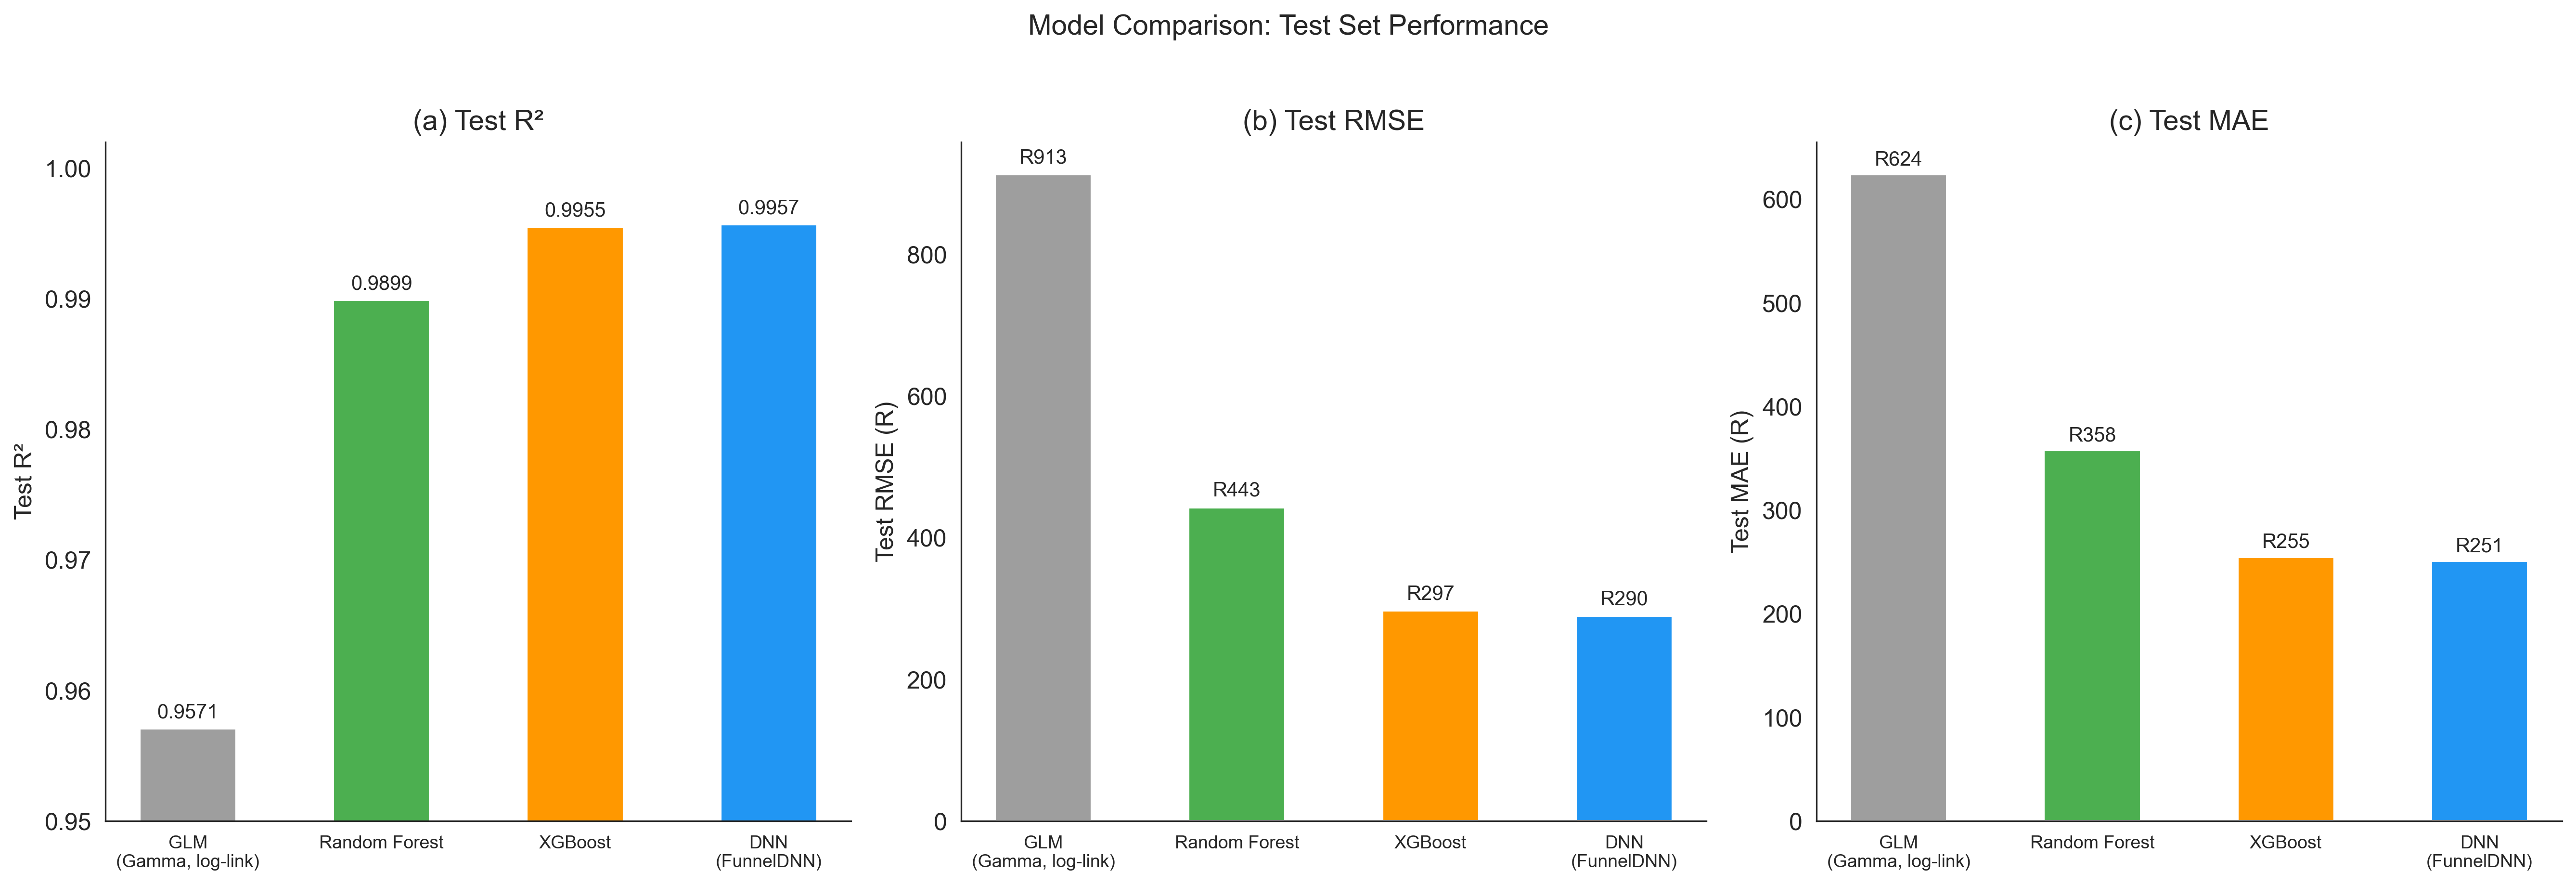
\includegraphics[width=0.9\textwidth]{Thesis/Chapter 4/Figures/fig_full_model_comparison.png}
    \caption{Full model comparison.}
    \label{fig:annexure_full_model_comparison}
\end{figure}


\clearpage
% =============================================================
% Annexure F: Code for Shapley-Value Computation
% =============================================================
\section{Code for Shapley-Value Computation}
\label{annexure:shapley}

% -------------------------------------------------------------
\subsection{SHAP GradientExplainer Setup}
\label{annexure:shap_setup}

\begin{lstlisting}[caption={SHAP GradientExplainer initialisation.}]
import copy
import shap
import torch
import numpy as np

# CPU copy for SHAP (faster than MPS for
# GradientExplainer)
model_cpu = copy.deepcopy(model).cpu()
model_cpu.eval()

# Background: 200 randomly sampled
# standardised training rows
rng = np.random.default_rng(SEED)
bg_idx = rng.choice(len(X_train_std),
                     200, replace=False)
X_bg = torch.tensor(X_train_std[bg_idx],
                    dtype=torch.float32)

# Foreground: all MC profiles (standardised)
X_mc_std = ((X_mc_encoded - X_mean) / X_std
            ).astype(np.float32)
X_fg = torch.tensor(X_mc_std,
                    dtype=torch.float32)

explainer = shap.GradientExplainer(
    model_cpu, X_bg)
\end{lstlisting}

% -------------------------------------------------------------
\subsection{Batch SHAP Computation}
\label{annexure:shap_batch}

\begin{lstlisting}[caption={Batch SHAP computation.}]
BATCH_SHAP = 2000
shap_values_list = []
n_batches = (B + BATCH_SHAP - 1) // BATCH_SHAP

for i in range(n_batches):
    start = i * BATCH_SHAP
    end = min((i + 1) * BATCH_SHAP, B)
    sv = explainer.shap_values(X_fg[start:end])

    if isinstance(sv, list):
        sv = sv[0]
    if isinstance(sv, torch.Tensor):
        sv = sv.cpu().numpy()
    # GradientExplainer returns shape (n, 22, 1)
    # for single-output models
    if sv.ndim == 3 and sv.shape[-1] == 1:
        sv = sv.squeeze(-1)

    shap_values_list.append(sv)

shap_values_22 = np.concatenate(
    shap_values_list, axis=0)
# shape: (10000, 22)
\end{lstlisting}

% -------------------------------------------------------------
\subsection{Efficiency Check}
\label{annexure:shap_efficiency}

\begin{lstlisting}[caption={SHAP efficiency verification.}]
with torch.no_grad():
    phi_0 = model_cpu(X_bg).mean().item()

with torch.no_grad():
    y_mc_norm = model_cpu(X_fg).numpy().flatten()

reconstructed = phi_0 + shap_values_22.sum(axis=1)
efficiency_error = np.abs(
    reconstructed - y_mc_norm)

print(f'phi_0 (base value): {phi_0:.6f}')
print(f'Mean |error|: {efficiency_error.mean():.6f}')
print(f'Max  |error|: {efficiency_error.max():.6f}')
print(f'Efficiency holds: '
      f'{efficiency_error.max() < 0.5}')
\end{lstlisting}

% -------------------------------------------------------------
\subsection{Dummy-to-Raw Aggregation}
\label{annexure:shap_aggregation}

\begin{lstlisting}[caption={Dummy-to-raw Shapley aggregation.}]
raw_to_encoded = {
    'age': [0],
    'gender': [1],
    'bmi': [2],
    'children': [3],
    'smoker': [4],
    'region': [5, 6, 7],
    'medical_history': [8, 9, 10],
    'family_medical_history': [11, 12, 13],
    'exercise_frequency': [14, 15, 16],
    'occupation': [17, 18, 19],
    'coverage_level': [20, 21]
}

RAW_VARS = list(raw_to_encoded.keys())

shap_values_11 = np.zeros(
    (B, 11), dtype=np.float32)
for j, (var_name, col_indices) in enumerate(
        raw_to_encoded.items()):
    shap_values_11[:, j] = (
        shap_values_22[:, col_indices].sum(axis=1))
\end{lstlisting}

% -------------------------------------------------------------
\subsection{Global Importance}
\label{annexure:shap_global}

\begin{lstlisting}[caption={Global SHAP importance.}]
mean_signed = shap_values_11.mean(axis=0)
mean_abs = np.abs(shap_values_11).mean(axis=0)

df_global_shap = pd.DataFrame({
    'Variable': RAW_VARS,
    'Mean Signed SHAP': mean_signed,
    'Mean |SHAP|': mean_abs
}).sort_values('Mean |SHAP|',
               ascending=False).reset_index(drop=True)

print(df_global_shap.to_string(index=False))
\end{lstlisting}

% -------------------------------------------------------------
\subsection{High-Cost Conditional Shapley Analysis}
\label{annexure:shap_conditional}

\begin{lstlisting}[caption={Conditional Shapley analysis.}]
thresholds = {'tau_90': 0.90,
              'tau_95': 0.95,
              'tau_99': 0.99}

u_vals = {}
h_sets = {}

for name, tau in thresholds.items():
    u = np.percentile(y_mc, tau * 100)
    mask = y_mc >= u
    u_vals[name] = u
    h_sets[name] = mask

conditional_results = {}

for name in ['tau_90', 'tau_95', 'tau_99']:
    mask = h_sets[name]
    sv_cond = shap_values_11[mask]

    cond_mean_signed = sv_cond.mean(axis=0)
    cond_mean_abs = np.abs(sv_cond).mean(axis=0)

    df_cond = pd.DataFrame({
        'Variable': RAW_VARS,
        'Cond Mean Signed': cond_mean_signed,
        'Cond Mean |SHAP|': cond_mean_abs
    }).sort_values('Cond Mean |SHAP|',
                   ascending=False
                   ).reset_index(drop=True)

    conditional_results[name] = df_cond
\end{lstlisting}



\clearpage
% =============================================================
% Annexure G: Additional Diagnostic Figures
% =============================================================
\section{Additional Diagnostic Figures}
\label{annexure:diagnostics}

% -------------------------------------------------------------
\subsection{Data Leakage Check Results}
\label{annexure:leakage}

\begin{enumerate}
    \item Split-before-preprocessing: PASS.
    \item Training-only standardisation: PASS.
    \item No target-derived predictor: PASS.
    \item Duplicate-row audit: PASS.
    \item Cross-partition leakage: PASS.
    \item Benchmark-dataset characterisation: PASS.
\end{enumerate}

% -------------------------------------------------------------
% -------------------------------------------------------------
\subsection{Partition Distribution Comparisons}
\label{annexure:partition_distributions}

\begin{figure}[H]
    \centering
    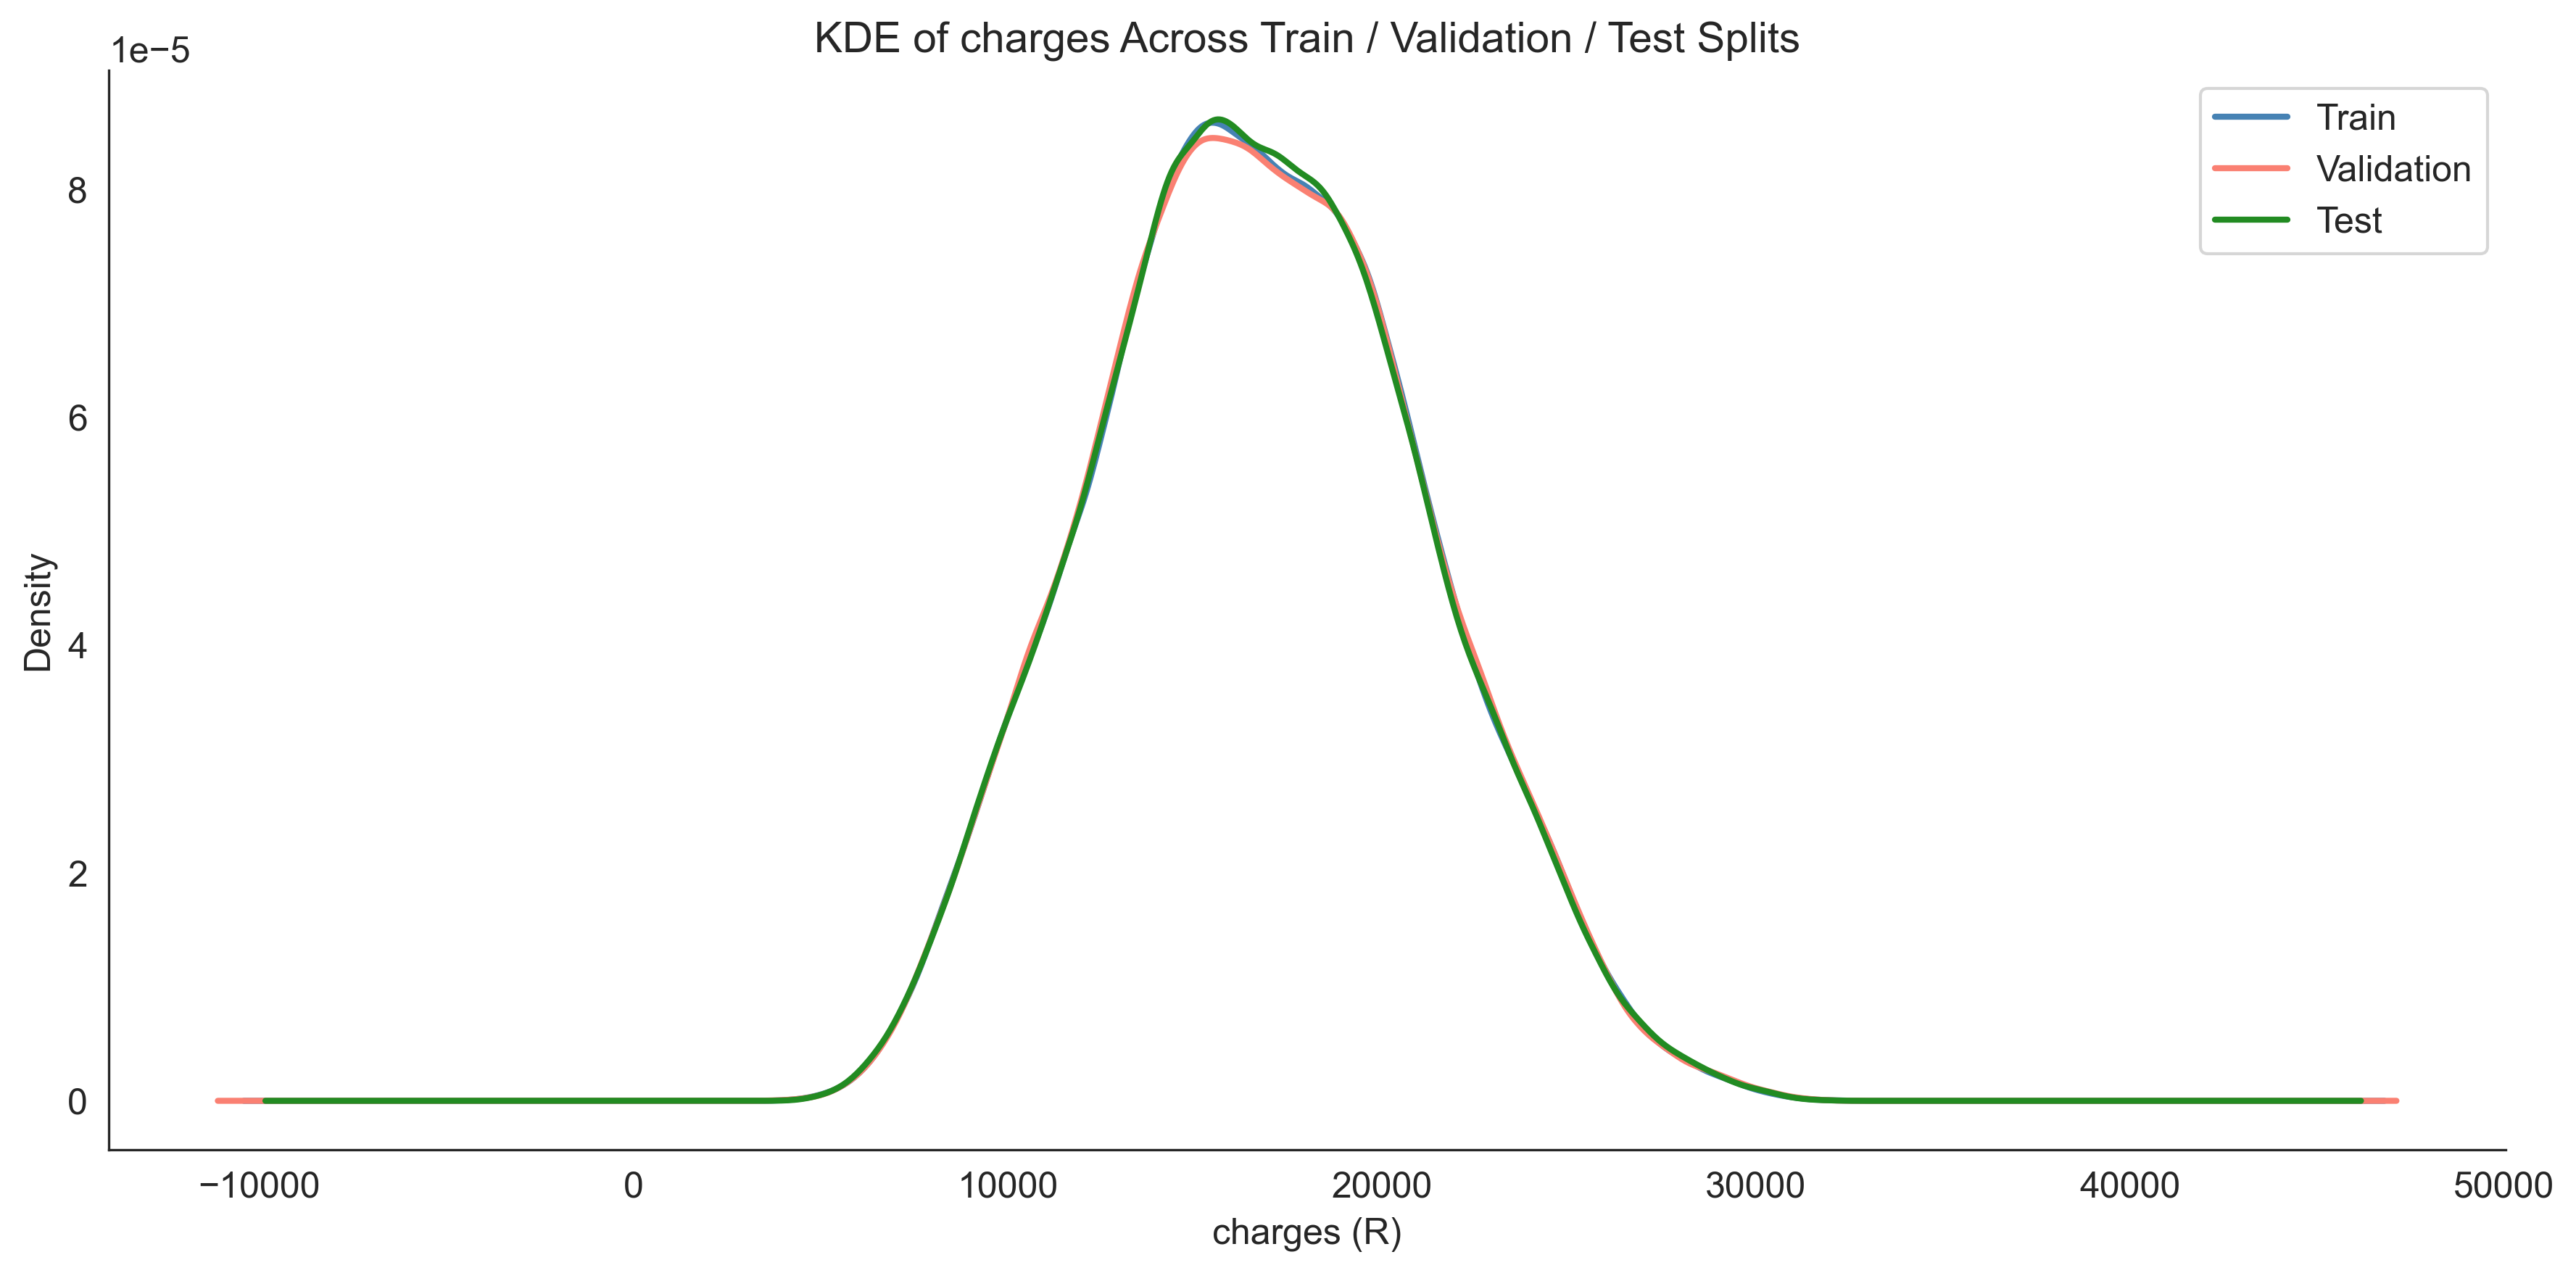
\includegraphics[width=\textwidth]{Thesis/Chapter 4/Figures/fig_split_charges_kde.png}
    \caption{Charges KDE across partitions.}
    \label{fig:annexure_split_charges}
\end{figure}

\begin{figure}[H]
    \centering
    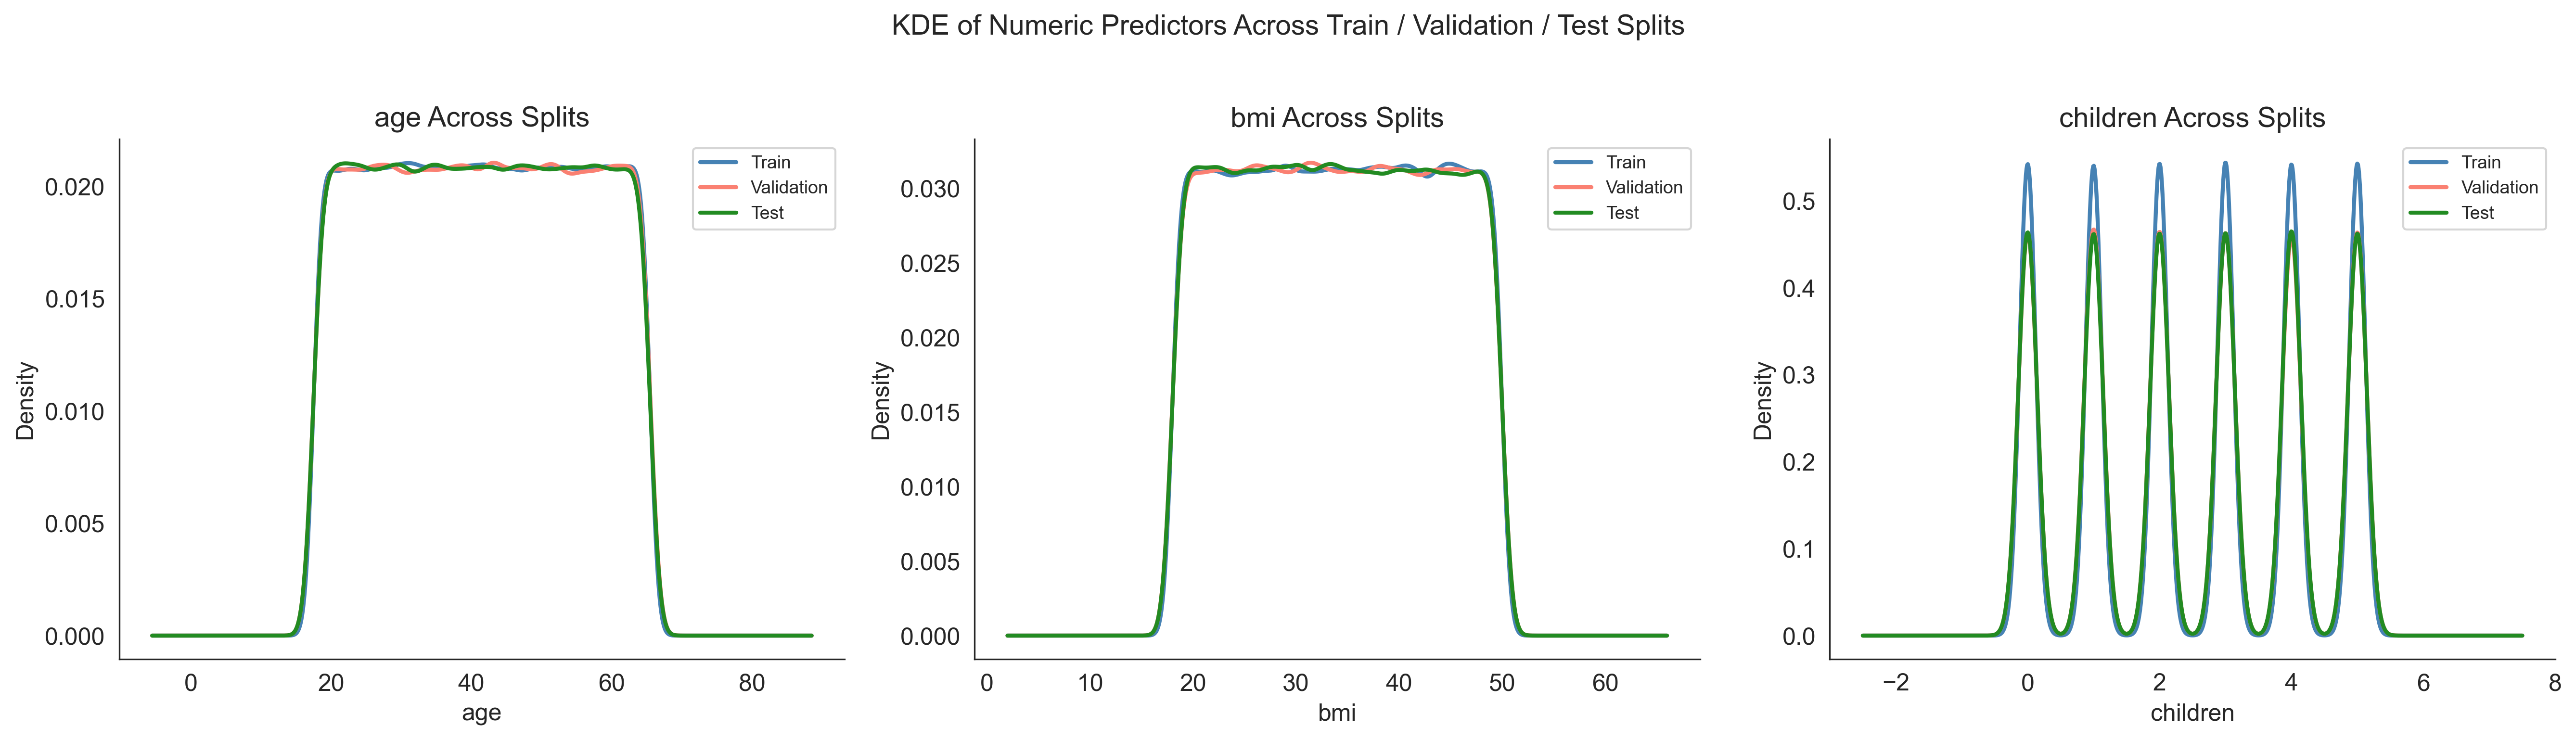
\includegraphics[width=\textwidth]{Thesis/Chapter 4/Figures/fig_split_numeric_kde.png}
    \caption{Numeric feature KDE across partitions.}
    \label{fig:annexure_split_numeric}
\end{figure}

\begin{figure}[H]
    \centering
    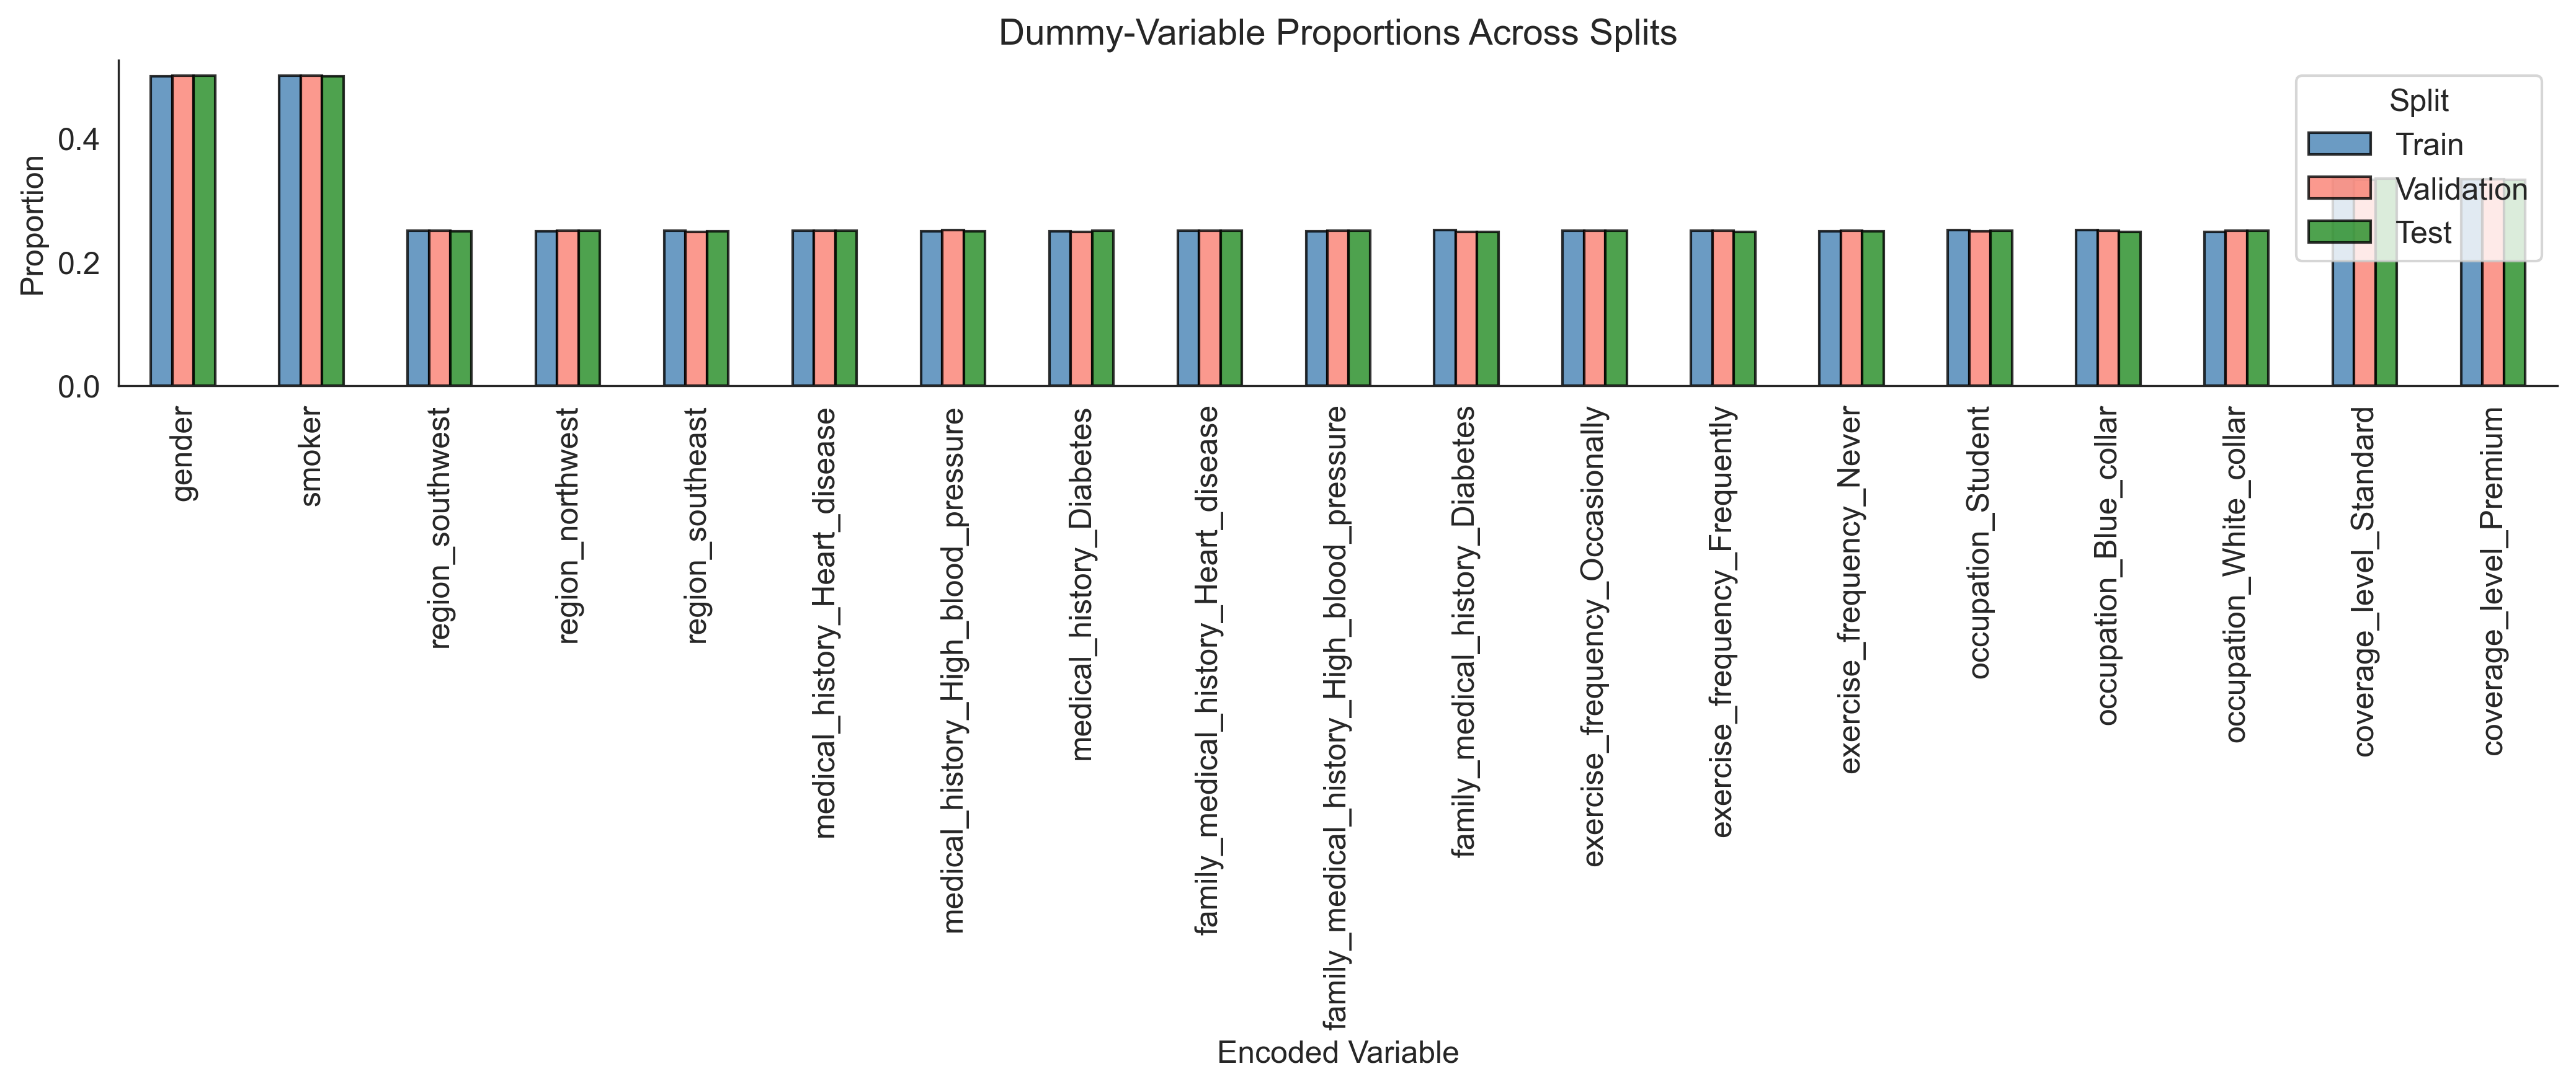
\includegraphics[width=\textwidth]{Thesis/Chapter 4/Figures/fig_split_dummy_proportions.png}
    \caption{Dummy variable proportions across partitions.}
    \label{fig:annexure_split_dummies}
\end{figure}


\clearpage
% =============================================================
% Annexure H: Full Hyperparameter Grid Results
% =============================================================
\section{Full Hyperparameter Grid Results}
\label{annexure:hyperparameters}

% -------------------------------------------------------------
\subsection{Five-Phase Sequential Comparison}
\label{annexure:five_phase}

Hyperparameters were selected through a five-phase sequential comparison procedure. In each phase, one hyperparameter was varied while all others were held at their current best values. The phases proceeded in the following order:

\begin{enumerate}
    \item Activation function (CELU, GELU, Tanh), with fixed lr${}=0.001$, batch size${}=256$, Adam.
    \item Learning rate ($0.01, 0.001, 0.0005, 0.0001$), with fixed best activation, batch size${}=256$, Adam.
    \item Batch size ($64, 128, 256, 512$), with fixed best activation and learning rate, Adam.
    \item Optimiser (Adam vs NAdam), with all previous best values fixed.
    \item Momentum $\beta_1$ ($0.90, 0.95, 0.99$) with $\beta_2 = 0.999$ fixed, using the best optimiser.
\end{enumerate}

Each configuration was trained with early stopping (patience of 10 validation checks at 5-epoch intervals) up to a maximum of 100 epochs. Table~\ref{tab:hyper_full} reports the full results.

\begin{table}[htbp]
\centering
\caption{Full five-phase hyperparameter comparison results.}
\label{tab:hyper_full}
\footnotesize
\begin{tabular}{llrrr}
\toprule
\textbf{Phase} & \textbf{Configuration} & \textbf{Best Epoch} & \textbf{Val $R^2$} & \textbf{Time (s)} \\
\midrule
\multirow{3}{*}{Phase 1: Activation}
  & CELU  & 100 & 0.995682 & 556.7 \\
  & GELU  &  25 & 0.995636 & 313.8 \\
  & Tanh  & 100 & 0.995532 & 565.9 \\
\midrule
\multirow{4}{*}{Phase 2: Learning Rate}
  & 0.01   &  10 & 0.995453 & 222.9 \\
  & 0.001  & 100 & 0.995682 & 558.1 \\
  & 0.0005 & 100 & 0.995692 & 563.8 \\
  & 0.0001 & 100 & 0.995686 & 556.0 \\
\midrule
\multirow{4}{*}{Phase 3: Batch Size}
  & 64  &  75 & 0.995678 & 1441.8 \\
  & 128 &  30 & 0.995669 &  491.9 \\
  & 256 & 100 & 0.995692 &  580.3 \\
  & 512 & 160 & 0.995685 &  487.3 \\
\midrule
\multirow{2}{*}{Phase 4: Optimiser}
  & Adam  & 100 & 0.995692 & 562.7 \\
  & NAdam &  85 & 0.995693 & 582.5 \\
\midrule
\multirow{3}{*}{Phase 5: Momentum}
  & $\beta_1=0.90$ & 85 & 0.995693 & 586.6 \\
  & $\beta_1=0.95$ & 40 & 0.995690 & 427.8 \\
  & $\beta_1=0.99$ & 95 & 0.995685 & 621.8 \\
\bottomrule
\end{tabular}
\end{table}

% -------------------------------------------------------------
\subsection{Phase Comparison Figures}
\label{annexure:phase_figures}

The following figures present the validation MSE loss and validation $R^2$
trajectories for each phase of the sequential hyperparameter comparison.

\begin{figure}[H]
\centering
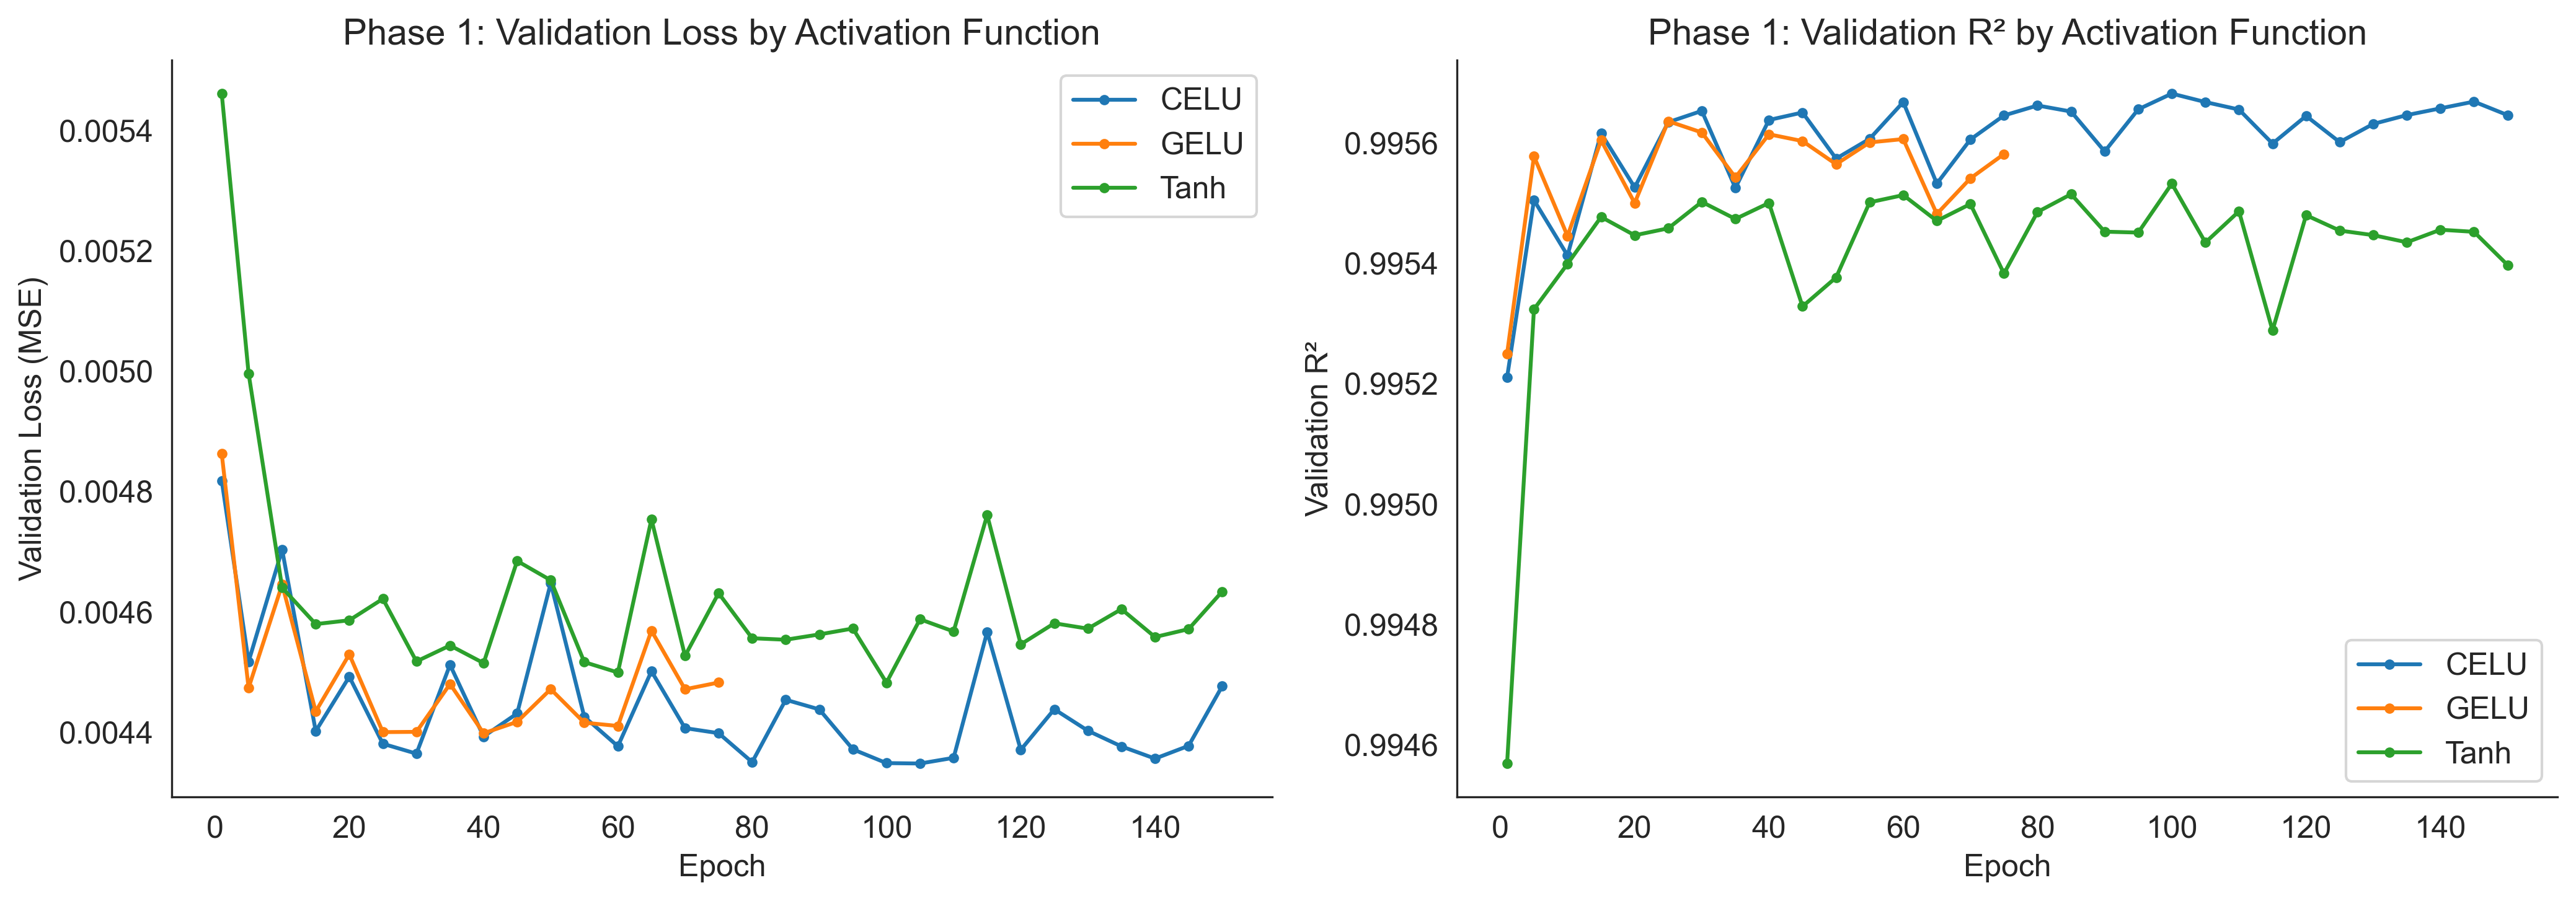
\includegraphics[width=0.95\textwidth]{Thesis/Chapter 4/Figures/fig_phase1_activation_comparison.png}
\caption{Phase~1: validation MSE loss (left) and validation $R^2$
(right) by activation function over training epochs.}
\label{fig:phase1_activation_annex}
\end{figure}

\begin{figure}[H]
\centering
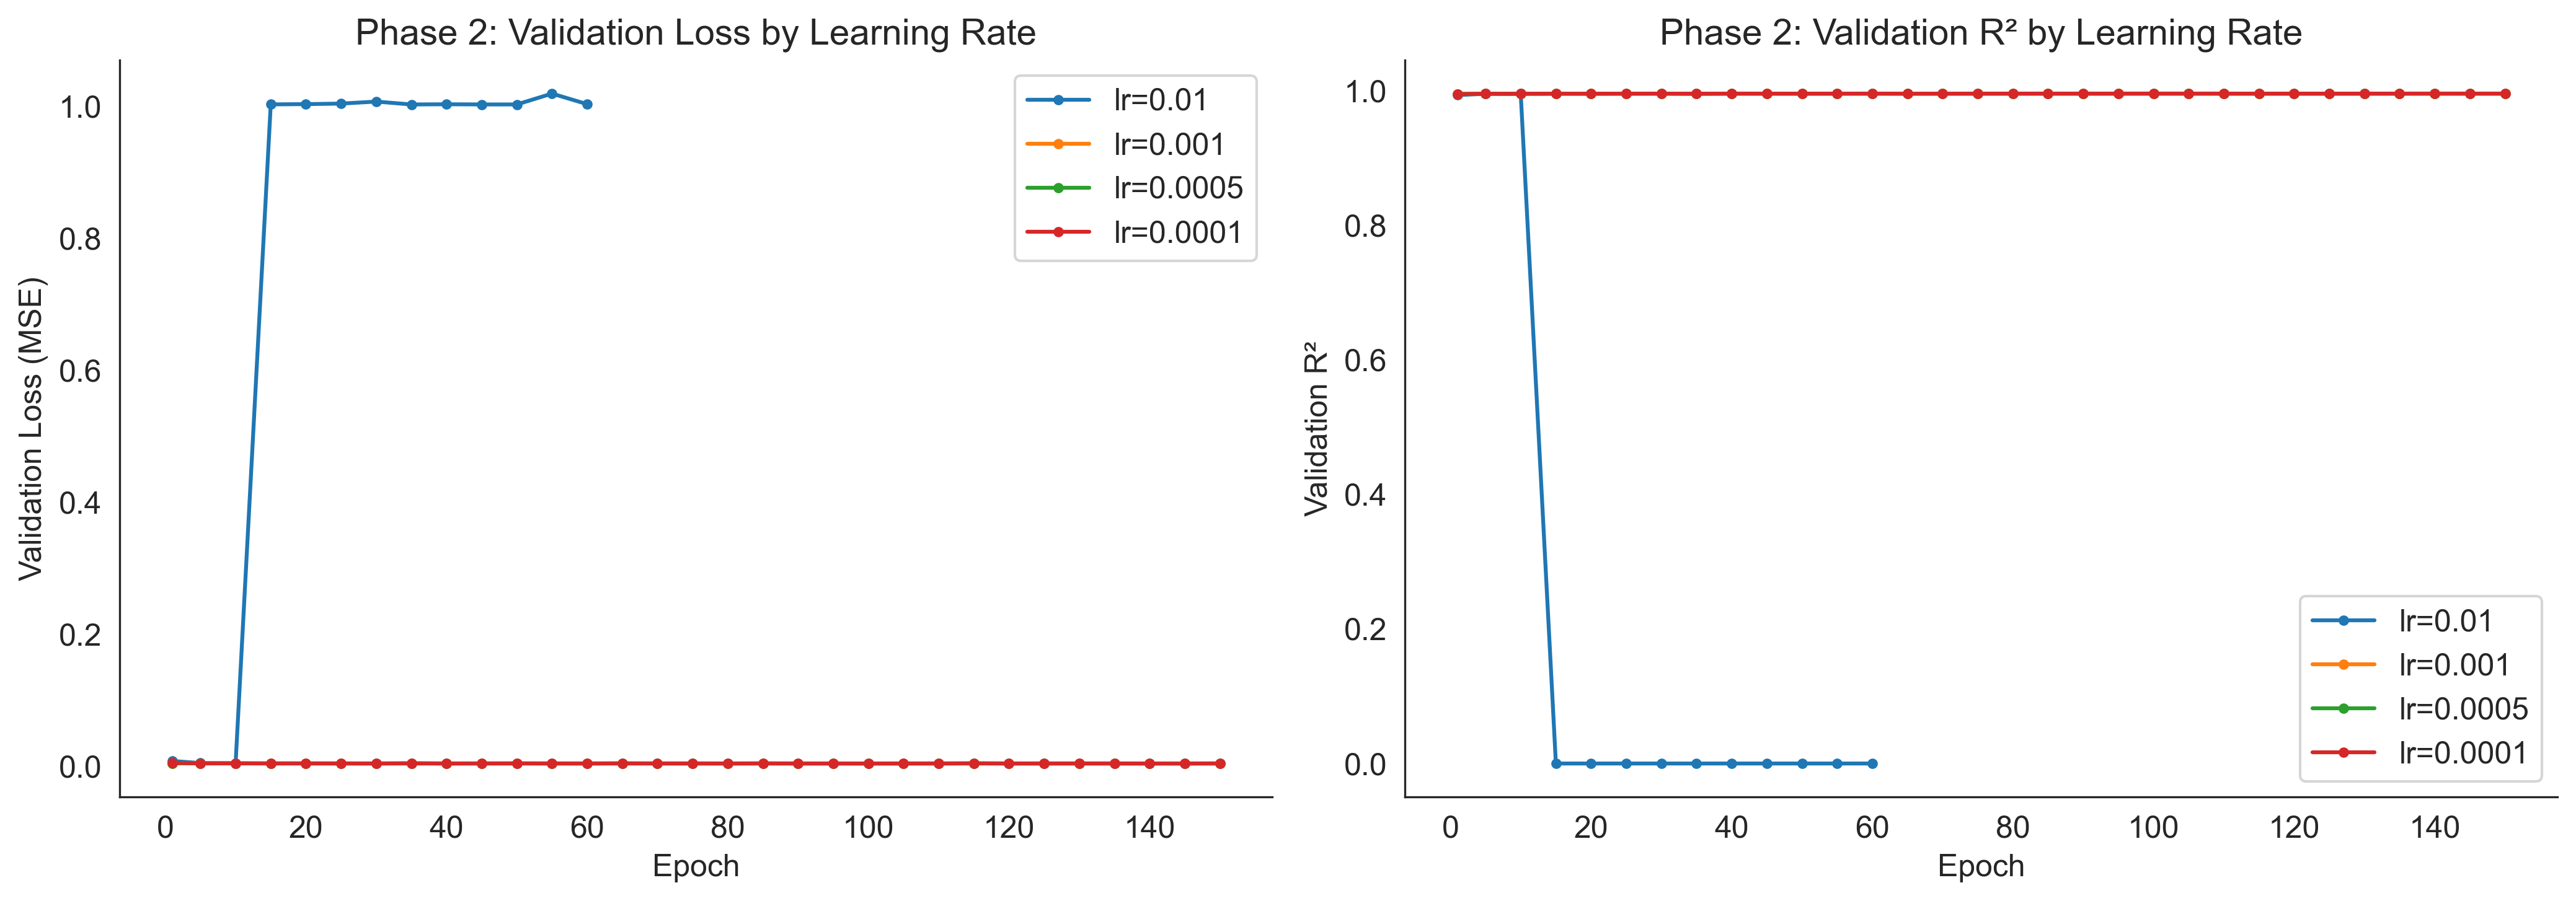
\includegraphics[width=0.95\textwidth]{Thesis/Chapter 4/Figures/fig_phase2_lr_comparison.png}
\caption{Phase~2: validation MSE loss (left) and validation $R^2$
(right) by learning rate.}
\label{fig:phase2_lr_annex}
\end{figure}

\begin{figure}[H]
\centering
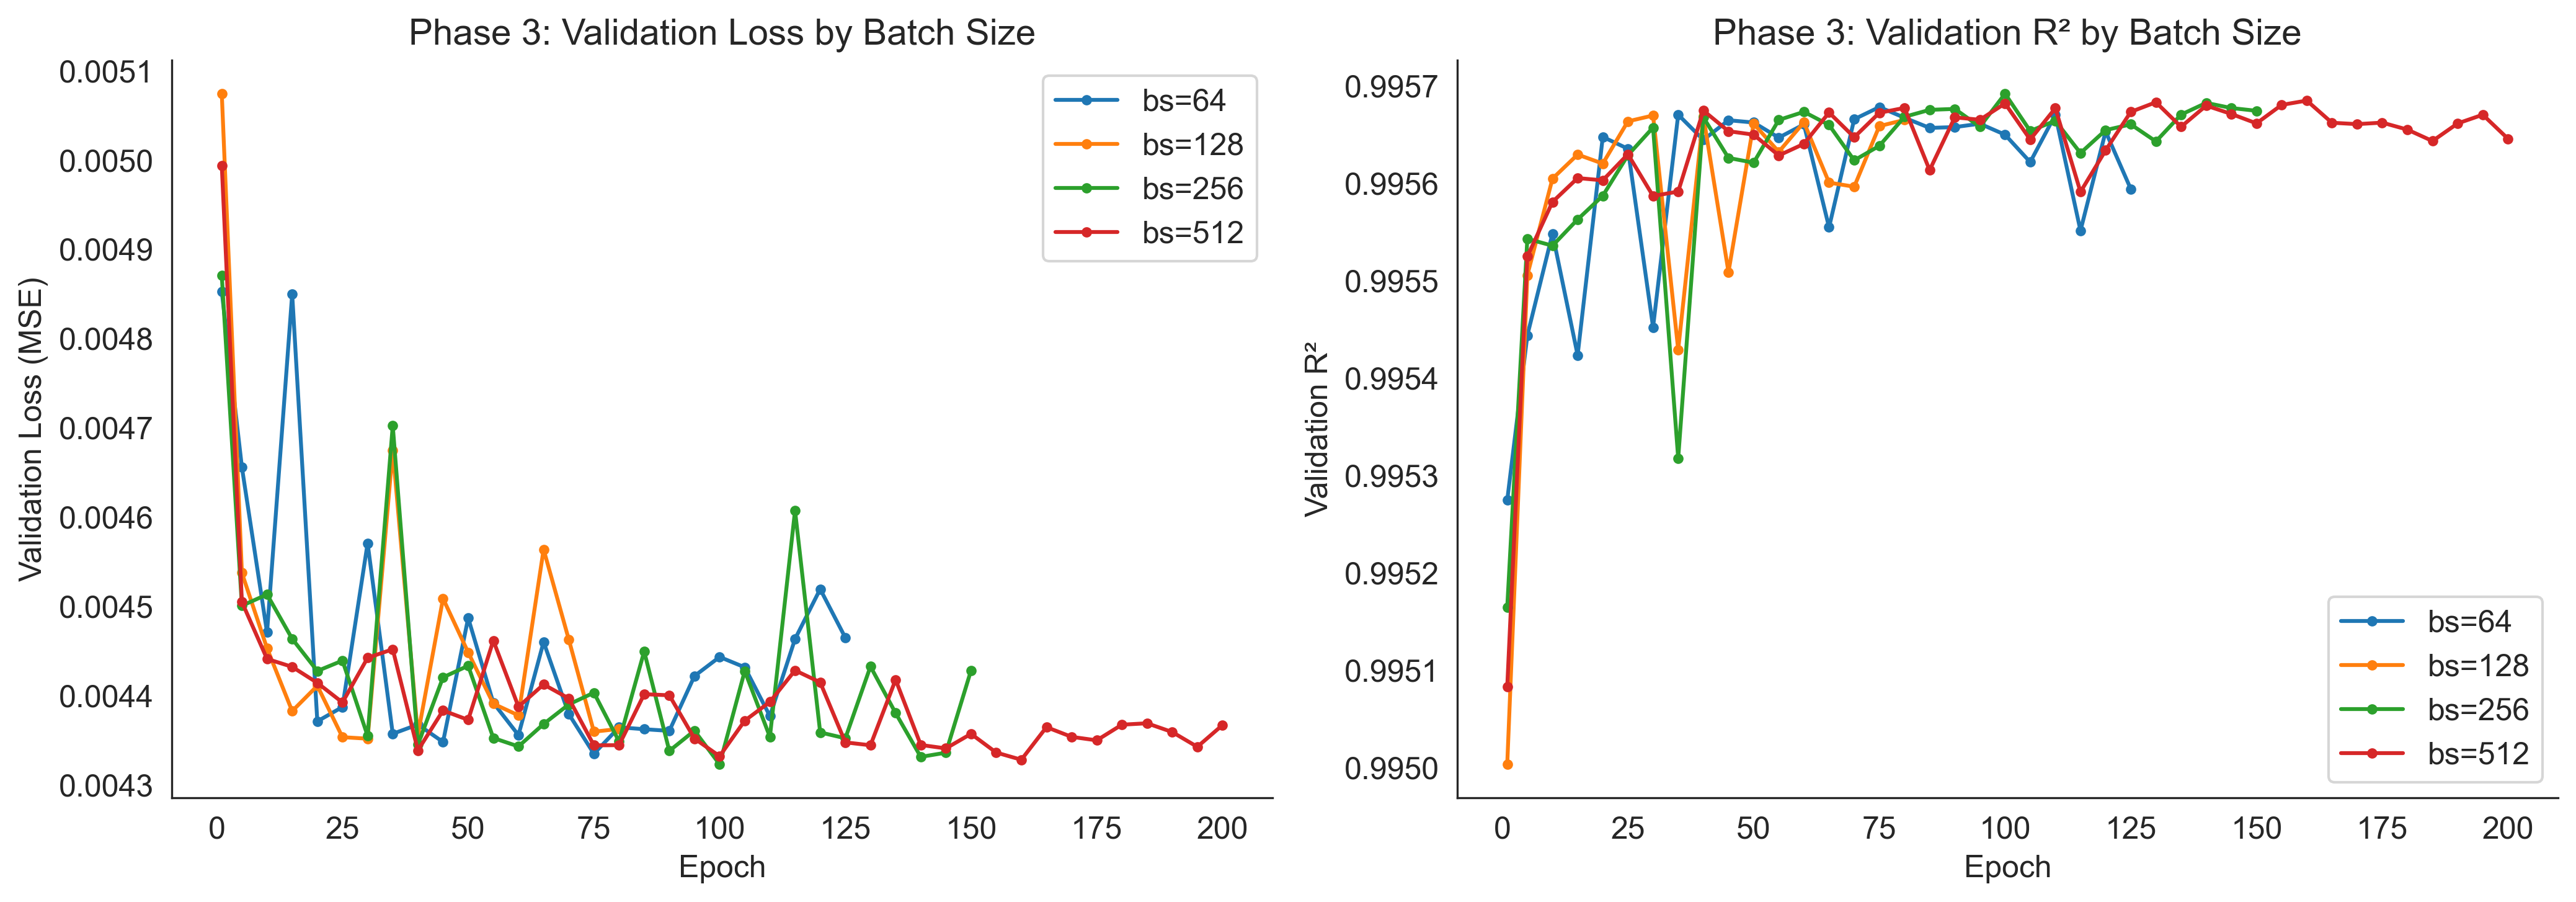
\includegraphics[width=0.95\textwidth]{Thesis/Chapter 4/Figures/fig_phase3_batchsize_comparison.png}
\caption{Phase~3: validation MSE loss (left) and validation $R^2$
(right) by batch size.}
\label{fig:phase3_batchsize_annex}
\end{figure}

\begin{figure}[H]
\centering
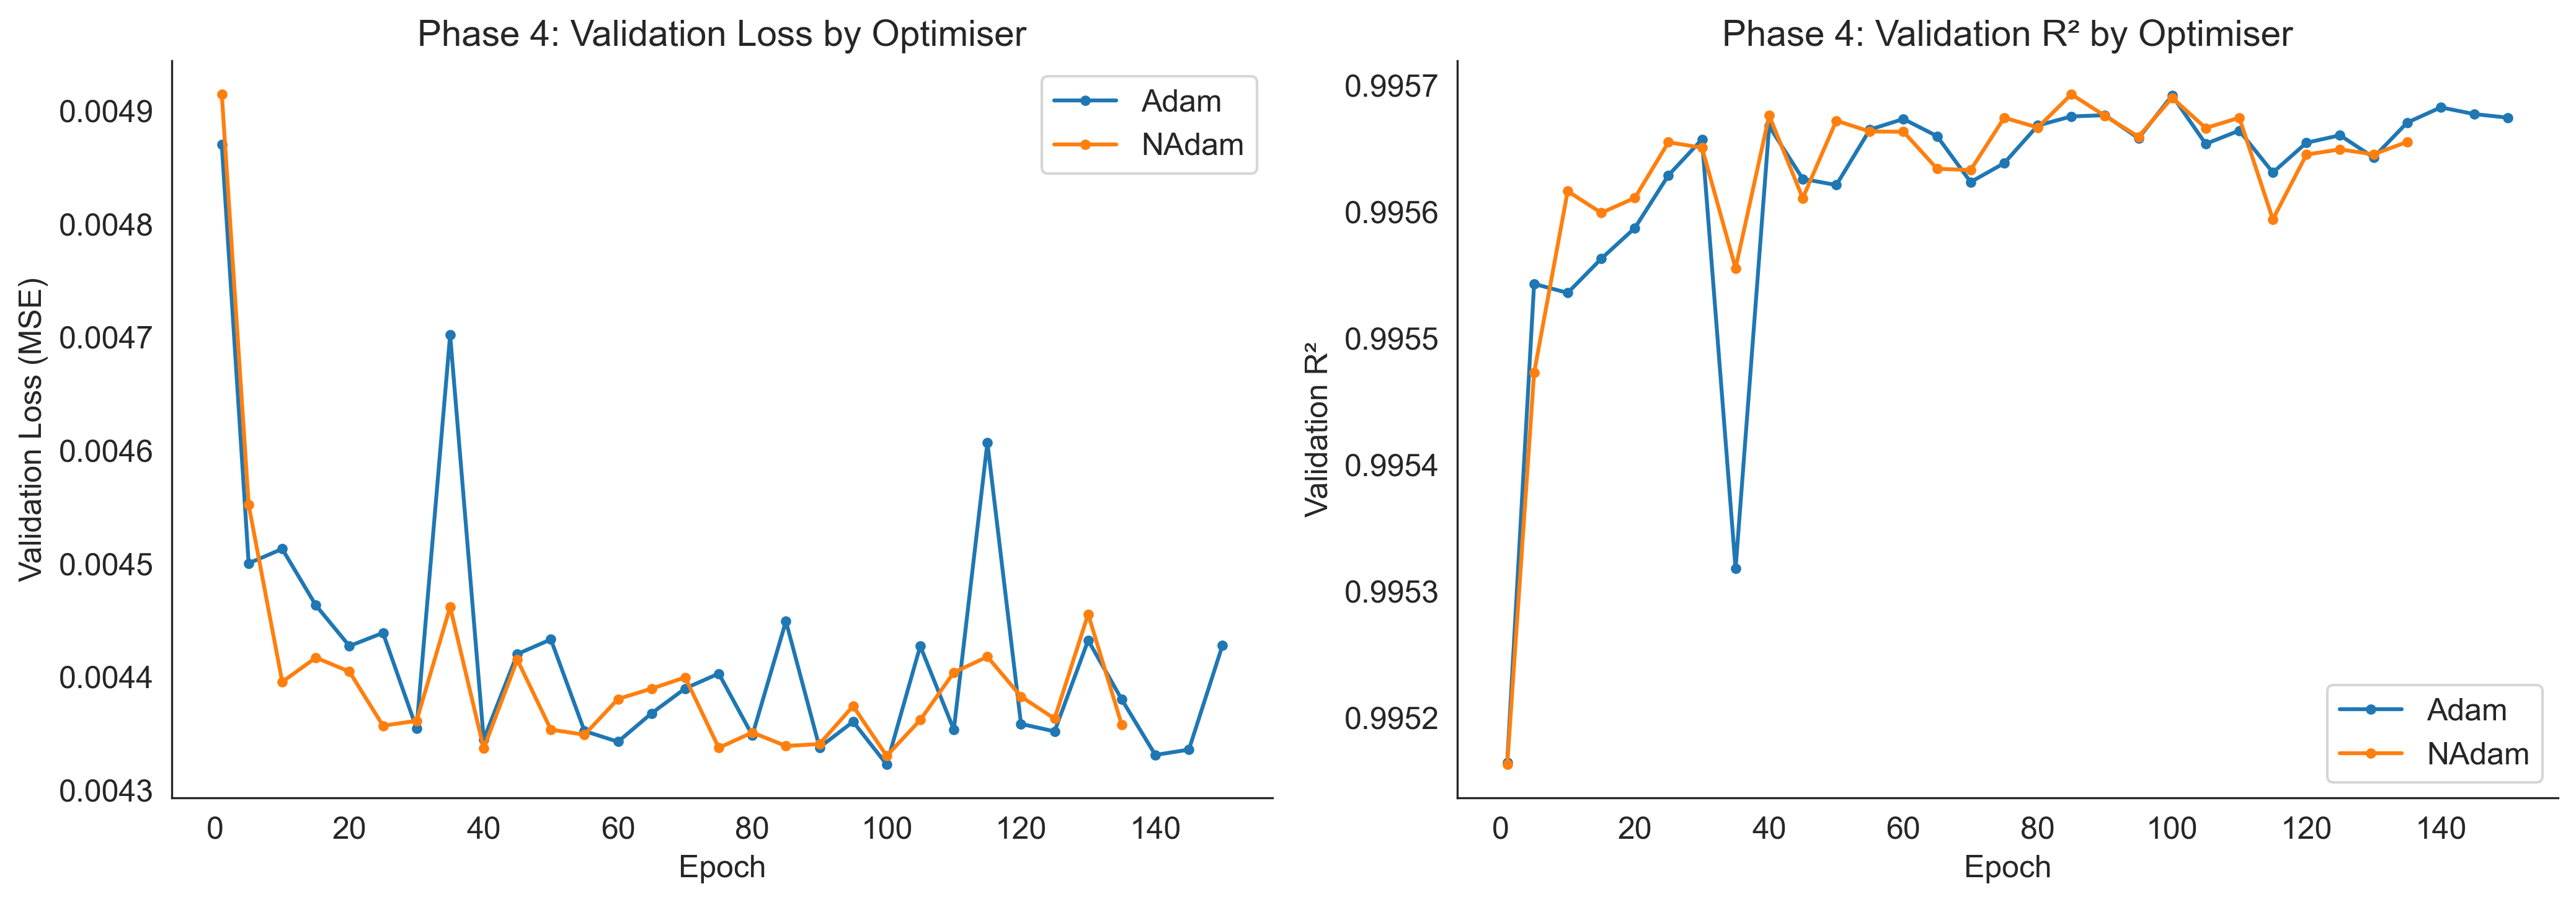
\includegraphics[width=0.95\textwidth]{Thesis/Chapter 4/Figures/fig_phase4_optimiser_comparison.png}
\caption{Phase~4: validation MSE loss (left) and validation $R^2$
(right) by optimiser.}
\label{fig:phase4_optimiser_annex}
\end{figure}

\begin{figure}[H]
\centering
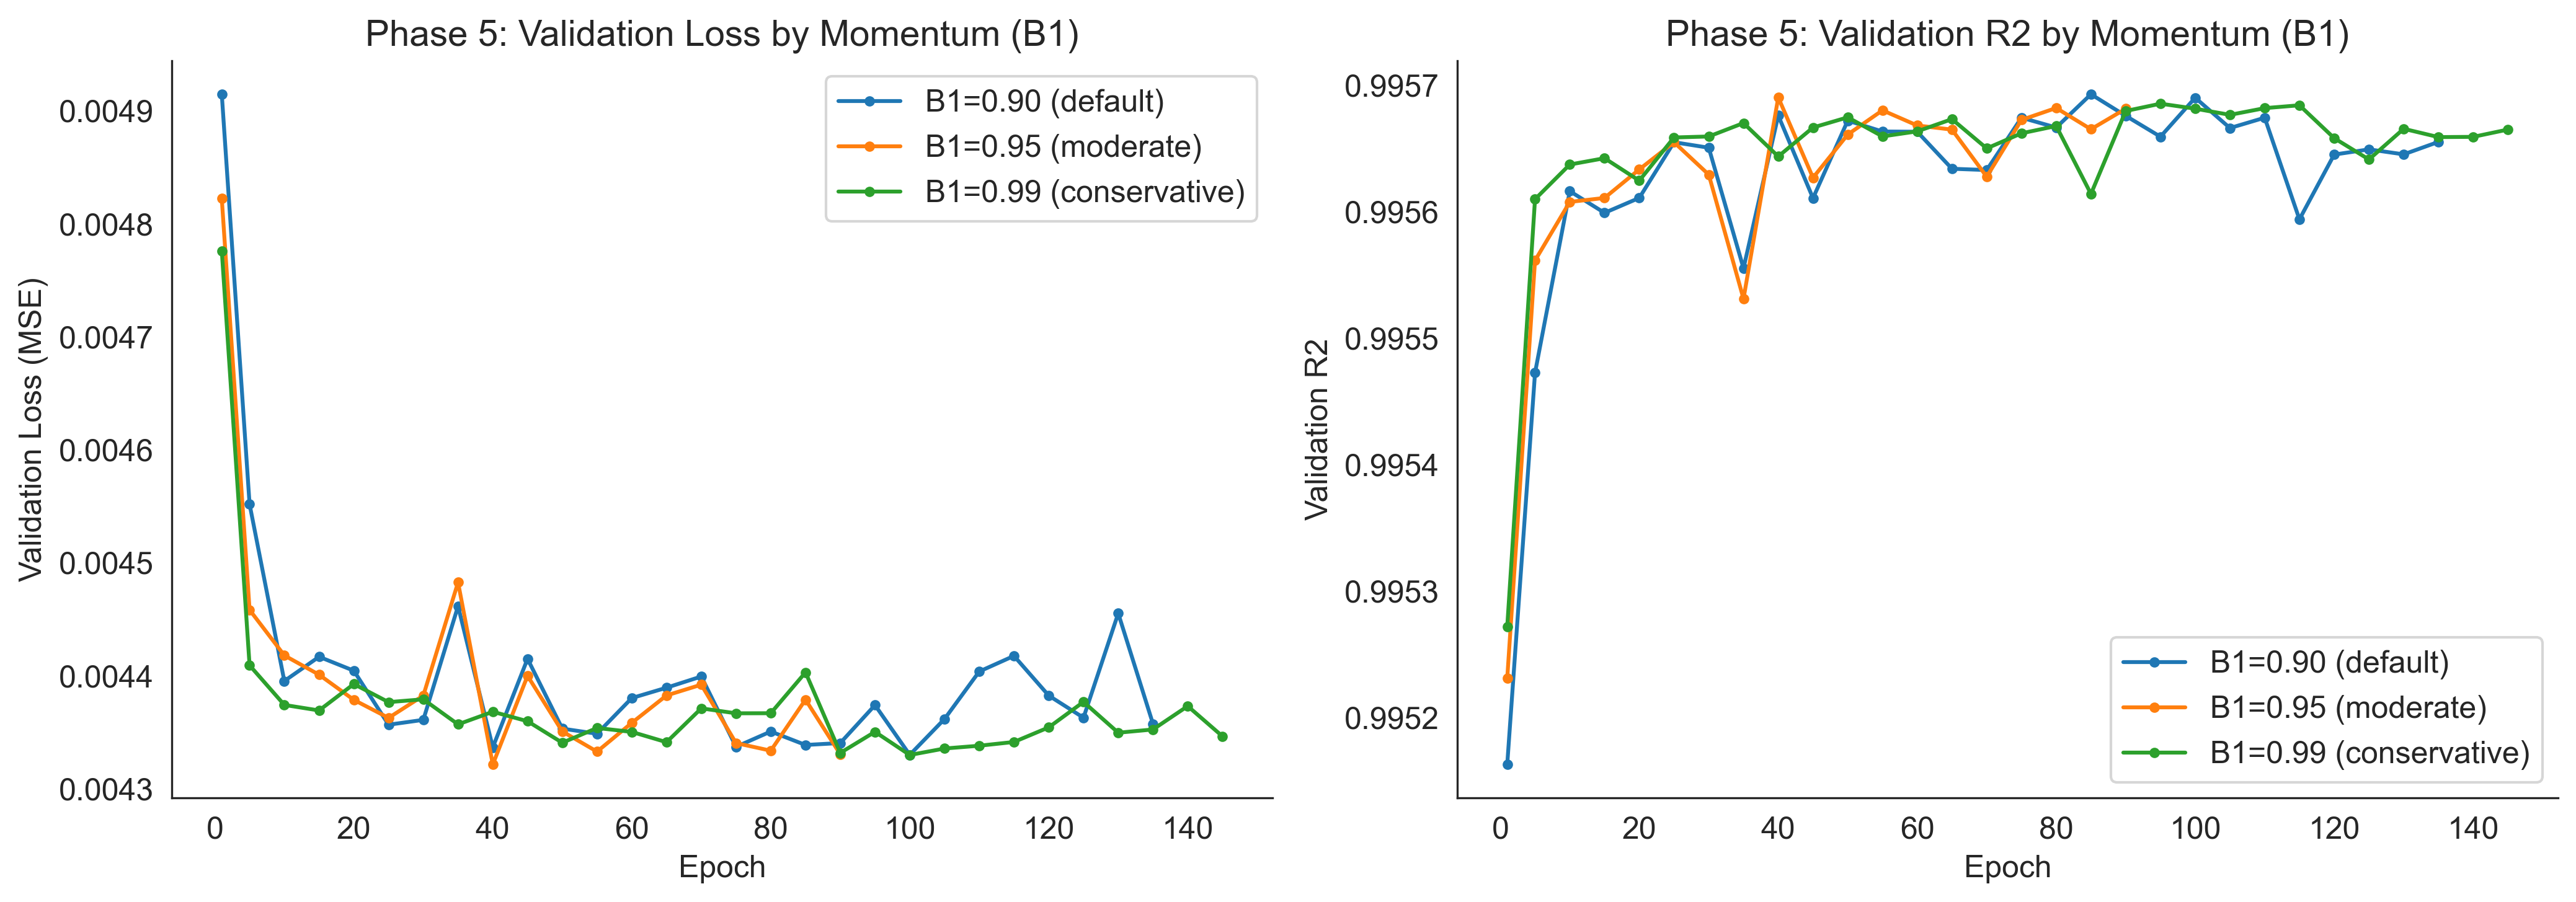
\includegraphics[width=0.95\textwidth]{Thesis/Chapter 4/Figures/fig_phase5_momentum_comparison.png}
\caption{Phase~5: validation MSE loss (left) and validation $R^2$
(right) by first momentum coefficient $\beta_1$.}
\label{fig:phase5_momentum_annex}
\end{figure}

\begin{figure}[H]
\centering
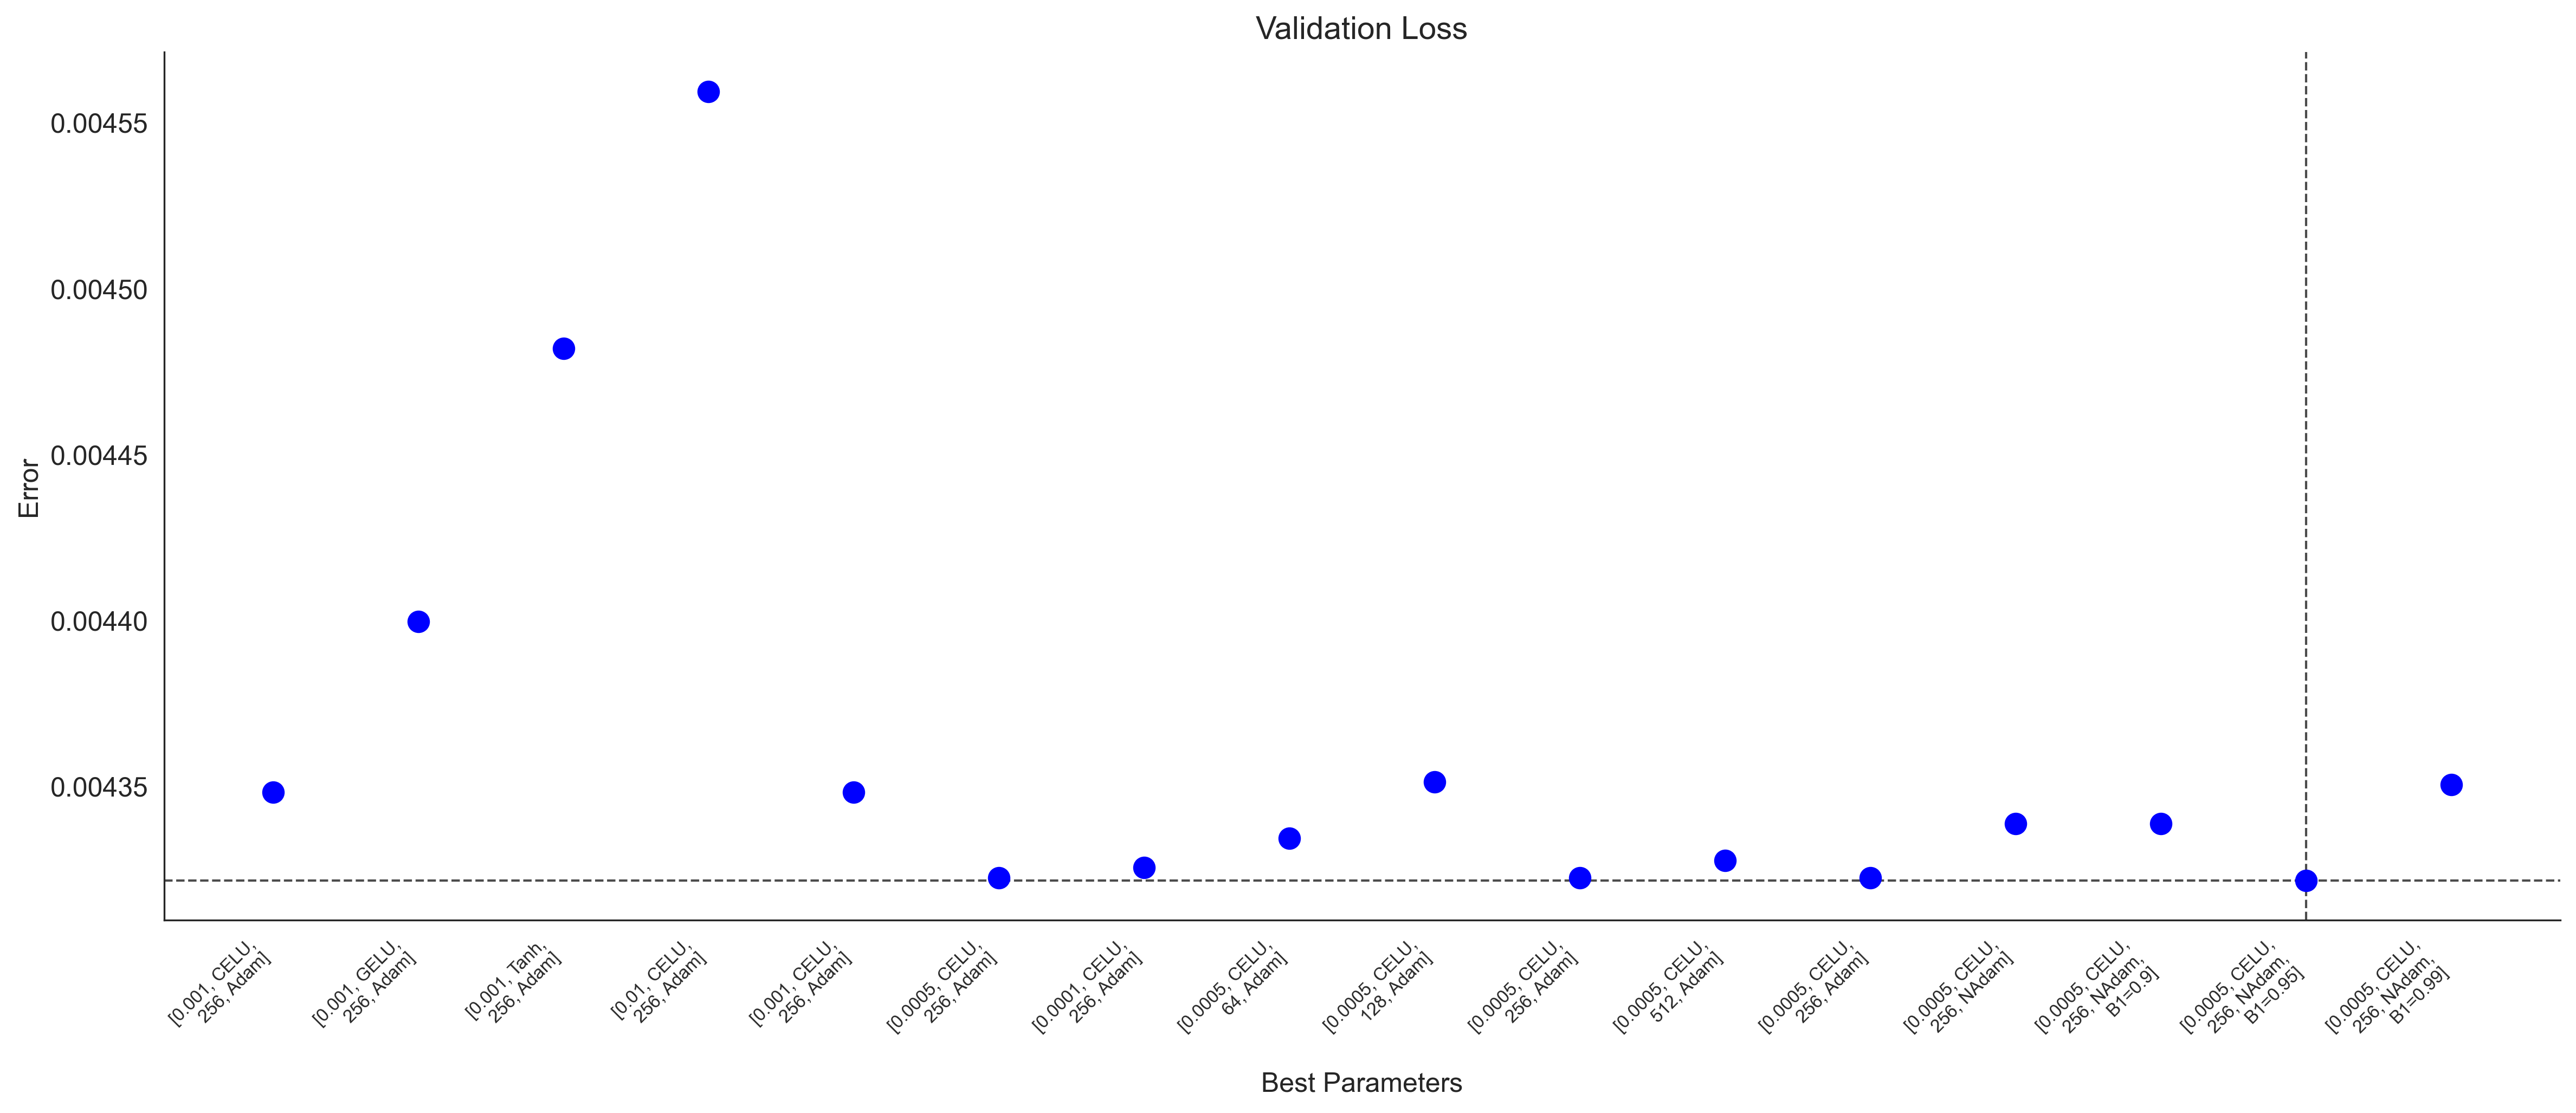
\includegraphics[width=0.95\textwidth]{Thesis/Chapter 4/Figures/fig_validation_loss_hyperparameters.png}
\caption{Best validation MSE loss across all hyperparameter
configurations evaluated in Phases~1 to~5.}
\label{fig:validation_loss_overview_annex}
\end{figure}

% -------------------------------------------------------------
\subsection{Bayesian Optimisation: GP Surrogate}
\label{annexure:bo_methodology}

A Gaussian process surrogate with a Mat\'{e}rn $\nu = 5/2$ kernel was fitted to the observed hyperparameter evaluations to visualise the validation-error landscape. The GP was fitted using scikit-learn's \texttt{GaussianProcessRegressor} with 15 random restarts, seed 42, and a composite kernel consisting of a constant kernel multiplied by the Mat\'{e}rn kernel plus a white noise kernel. Log-scaled axes were used for the learning rate dimension. The fitted surface and its uncertainty were evaluated on a $100 \times 100$ grid with 15\% margin beyond the observed range.

% -------------------------------------------------------------
\subsection{Consolidated Best Hyperparameter Summary}
\label{annexure:best_hyperparams}

\begin{table}[htbp]
\centering
\caption{Best hyperparameter configuration selected for the final DNN model.}
\label{tab:best_hyperparams}
\begin{tabular}{ll}
\toprule
\textbf{Hyperparameter} & \textbf{Selected Value} \\
\midrule
Architecture    & $22 \to 256 \to 128 \to 64 \to 32 \to 16 \to 1$ \\
Activation      & CELU \\
Learning rate   & 0.0005 \\
Batch size      & 256 \\
Optimiser       & NAdam \\
$\beta_1$       & 0.90 \\
$\beta_2$       & 0.999 \\
Bias            & False (all layers) \\
Max epochs      & 100 \\
Early stopping  & 10 checks (every 5 epochs) \\
Loss function   & MSE (on normalised scale) \\
\bottomrule
\end{tabular}
\end{table}



\clearpage
% =============================================================
% Annexure I: Software and Environment Details
% =============================================================
\section{Software and Environment Details}
\label{annexure:software}


% -------------------------------------------------------------
\subsection{Python Distribution and Version}
\label{annexure:python}

Python~3.11 via the Anaconda distribution. Jupyter Notebook was used for interactive development.

% -------------------------------------------------------------
\subsection{Core Package Versions}
\label{annexure:packages}

\begin{table}[htbp]
\centering
\caption{Python package versions used in the dissertation.}
\label{tab:packages}
\begin{tabular}{lll}
\hline
\textbf{Package} & \textbf{Version} & \textbf{Purpose} \\
\hline
PyTorch           & 2.x              & DNN architecture, training and inference \\
SHAP              & 0.43+            & Shapley value computation (GradientExplainer) \\
statsmodels       & 0.14+            & GLM (Gamma, log-link) fitting \\
NumPy             & 1.24+            & Numerical computation \\
pandas            & 2.x              & Data manipulation and I/O \\
SciPy             & 1.11+            & Statistical tests, distributions \\
scikit-learn      & 1.3+             & GP surrogate, train/test splitting, metrics \\
matplotlib        & 3.8+             & Static figure generation \\
seaborn           & 0.13+            & Statistical visualisation \\
scikit-optimize   & 0.10+            & Bayesian Optimisation (\texttt{gp\_minimize}) \\
Plotly            & 5.x              & Interactive 3D surface plots \\
\hline
\end{tabular}

\medskip
\emph{Note:} Exact patch versions may vary. The versions above represent the minimum versions with which the code was tested. Update these entries with the output of \texttt{pip freeze} or \texttt{conda list} before final submission.
\end{table}

% -------------------------------------------------------------
\subsection{Hardware Platform}
\label{annexure:hardware}

\begin{itemize}
    \item Processor: Apple Silicon (M-series)
    \item Primary compute device: MPS (Metal Performance Shaders) via PyTorch
    \item SHAP compute device: CPU (faster than MPS for GradientExplainer)
    \item Fallback: CPU (used when MPS is unavailable or for SHAP computations)
\end{itemize}

\begin{lstlisting}[caption={Device selection logic for PyTorch.}]
import torch

if torch.backends.mps.is_available():
    DEVICE = torch.device('mps')
elif torch.cuda.is_available():
    DEVICE = torch.device('cuda')
else:
    DEVICE = torch.device('cpu')
\end{lstlisting}

% -------------------------------------------------------------
\subsection{Reproducibility}
\label{annexure:reproducibility}

Fixed random seed of 42:
\begin{itemize}
    \item PyTorch weight initialisation (\texttt{torch.manual\_seed(42)})
    \item NumPy random operations (\texttt{np.random.seed(42)})
    \item NumPy Generator objects (\texttt{np.random.default\_rng(42)})
    \item scikit-learn train/test split (\texttt{random\_state=42})
    \item GP surrogate fitting (\texttt{random\_state=42})
\end{itemize}

% -------------------------------------------------------------
\subsection{Data Files}
\label{annexure:data_files}

\begin{itemize}
    \item \texttt{insurance\_dataset.csv}: 1\,000\,000 rows, 12 columns (age, gender, bmi, children, smoker, region, medical\_history, family\_medical\_history, exercise\_frequency, occupation, coverage\_level, charges). Synthetic benchmark dataset sourced from Kaggle.

    \item \texttt{chapter3\_final\_model.pth}: PyTorch checkpoint containing the trained FunnelDNN model state, architecture specification, hyperparameters, standardisation parameters, feature names and evaluation metrics.

    \item \texttt{model\_ready\_charges\_train\_20260517\_115748.csv}: reference-category encoded training partition (60\% of the dataset, 22 features + charges).
\end{itemize}


\end{document}